\documentclass[ a4paper,	%Pour papier A4
   %b5paper,	%Pour papier B5
   12pt,		%Taille de la police 12
   twoside,	%recto-verso
   headinclude, headsepline, plainheadsepline,
   bibliography=totoc, toc=listof,
   numbers=noenddot,
   captions=tableheading,
   % fleqn,   % left alignment of formula
   amsmath, hidelinks ]{book}
\usepackage{graphicx} % Required for inserting images
 \usepackage{ragged2e}

\usepackage{lipsum}
	
\usepackage{pdfpages}

\usepackage{bold-extra}
\usepackage[french]{babel}
\usepackage[T1]{fontenc} 
\usepackage[utf8]{inputenc} 
\usepackage[singlespacing]{setspace}

\usepackage{bm, amsmath,amssymb,color,sistyle}
 \usepackage{multirow}
\usepackage{cprotect}
\usepackage{wrapfig}
\usepackage{footmisc}
\usepackage{subcaption}

\usepackage[makeroom]{cancel}

%\usepackage[square,sort,authoryear]{natbib}
\usepackage{csquotes}
\usepackage[
   backend=biber,        % compilateur par défaut pour biblatex
   sorting=nyt,          % trier par nom, année, titre
   citestyle=authoryear, % style de citation auteur-année
   bibstyle=science,
   %bibstyle=vancouver,  % style de bibliographie alphabétique
   isbn=false, url=false, doi=false, eprint=false,
   uniquename=false,
   date=year,
]{biblatex}
\addbibresource{biblio.bib}
%\usepackage{hyperref}

\DefineBibliographyStrings{french}{%
  pages = {pp\adddot},
  in ={\emph{in}},
  volume={vol\adddot\addspace},
  number={\no}
}
\AtEveryBibitem{%
  \clearfield{note}%
}

\DeclareFieldFormat{no}{\bibsstring{number}#1}
\DeclareFieldFormat{vol}{\bibsstring{volume}#1}

\renewbibmacro*{volume+number+eid}{%
  \addcomma\addspace%
  \printfield[vol]{volume}%
  \setunit{\addcomma\addspace}%
  \printfield[no]{number}%
  \setunit{\addcomma\addspace}%
  \printfield{eid}
}

\usepackage{set_format}
\usepackage{Metadata/infos}
\usepackage{Special/pages_speciales}
\usepackage{Special/lists}
\usepackage{Special/todo}



\begin{document}
%\usepackage{xspace}
%\xspaceaddexceptions{]\}}
%Uncomment next line if AMS fonts required
%\usepackage{iopams}

%========================
% Nomenclature

%% This code creates the groups
% -----------------------------------------

\renewcommand\nomgroup[1]{%
  \item[
  \ifstrequal{#1}{P}{{\bf Constantes et paramètres physiques}}{%
  \ifstrequal{#1}{N}{{\bf Paramètres numériques}}{%
  \ifstrequal{#1}{R}{{\bf Systèmes de représentation}}{
  \ifstrequal{#1}{Q}{{\bf Quantités}}{
  \ifstrequal{#1}{O}{{\bf Opérateurs et opérations} (exemples donnés entre quantités indéfinies \ensuremath{A}, \ensuremath{B}).}{
  }}}}}%
]}

% This will add the units
%----------------------------------------------
\newcommand{\nomunit}[1]{%
\renewcommand{\nomentryend}{\hspace*{\fill}#1}}
%----------------------------------------------

%nomenclature text 
\renewcommand{\nompreamble}{La liste suivante contient les notations utilisées récurrament dans l'ensemble de cette thèse ainsi que quelques éléments de définition. L'usage courant des notations est généralement respecté et sauf unités spécifiques utilisées dans la communauté astrophysique, les unités sont exprimées dans le système international (SI). 
Les vecteurs sont notés en gras, les tenseurs en gras surmontés d'une (ordre 2) ou deux barres (ordre 3).
Les quantités liées à l'écoulement sont indicées par $\alpha$, $e$, $i$ si une distinction est faite sur le type de particules s'écoulant (resp. espèce quelconque mais distincte, électrons, ions). Les valeurs moyennes sont en générale indicées par un $0$ et les fluctuations linéaires par un $1$ si requis (exemple dans le cadre des linéarisations). Dans les études de turbulence, les quantités exprimées en $\mathbf{x'}$ sont primés. 

 }

% Paramètres physiques
\nomenclature[P]{\ensuremath{e}}{charge élémentaire. \nomunit{$\SI{1.602176634e-19}{C}$}}
\nomenclature[P]{\ensuremath{m_p}}{masse d'un proton. \nomunit{$\SI{ 1.6726e-27 }{kg}$}}
\nomenclature[P]{\ensuremath{m_i}}{masse ionique proportionnelle à \ensuremath{m_p}.}
\nomenclature[P]{\ensuremath{m_e}}{masse d'un électron. \nomunit{$\SI{9.1094e-31 }{kg}$}}
\nomenclature[P]{\ensuremath{\mu}}{rapport massique \ensuremath{m_e/m_i}.}
\nomenclature[P]{\ensuremath{\nu}}{viscosité du fluide, caractérise la dissipation cinétique. }
\nomenclature[P]{\ensuremath{\eta}}{résistivité du fluide, caractérise la diffusivité magnétique.}
\nomenclature[P]{\ensuremath{a_p}}{taux d'anisotropie de pression, correspond à une pression perpendiculaire sur une pression parallèle.}
\nomenclature[P]{\ensuremath{R_e}}{nombre de Reynolds, rapport entre convection et dissipation cinétique (voir section \ref{sec-011}).}
\nomenclature[P]{\ensuremath{R_m}}{nombre de Reynolds magnétique, rapport entre convection et diffusivité magnétique (voir section \ref{sec-011}).}
\nomenclature[P]{\ensuremath{\beta}}{paramètre du plasma, correspond à une pression sur la pression magnétique, indicé suivant le type de pression (ex. : \ensuremath{\beta_{\parallel} = p_{\parallel}/p_m}).}
\nomenclature[P]{\ensuremath{\epsilon_0}}{permittivité du vide. \nomunit{$\SI{8.854e-12}{A^2 .s^4 .kg^{-1} .m^{-3}}$}}
\nomenclature[P]{\ensuremath{\mu_0}}{perméabilité (magnétique) du vide, \ensuremath{1/(\epsilon_0 c^2)}.}
\nomenclature[P]{\ensuremath{c}}{vitesse de la lumière dans le vide. \nomunit{$\SI{2.99 792 458 e8}{ m s^{-1}}$}}
\nomenclature[P]{\ensuremath{d_{i,e}}}{longueur d'inertie ionique (resp. électronique).}
\nomenclature[P]{\ensuremath{\rho_{Li,Le}}}{rayon de Larmor ionique (resp. électronique).}
\nomenclature[P]{\ensuremath{q_{\alpha}}}{charge particulaire, à ne pas confondre avec les flux de chaleurs.}
\nomenclature[P]{\ensuremath{\omega_{ci,ce}}}{pulsation cyclotron ionique (resp. électronique).}
\nomenclature[P]{\ensuremath{\lambda_{i,e}}}{rapport masse-charge élémentaire des ions et électrons}
\nomenclature[P]{\ensuremath{\lambda_{c}}}{longueur de corrélation.}
\nomenclature[P]{\ensuremath{au}}{unité atronomique, distance Soleil-Terre. \nomunit{$\SI{1.49597870700 e-11 }{m}$}} 
\nomenclature[P]{\ensuremath{Rs}}{rayon solaire. \nomunit{$\SI{6.958 e-8 }{m}$}} 

% Variables
\nomenclature[Q]{\ensuremath{t}}{instant, temps.}
\nomenclature[Q]{\ensuremath{f}}{fréquence temporelle.}
\nomenclature[Q]{\ensuremath{\mathbf{x}}}{position.}
\nomenclature[Q]{\ensuremath{\mathbf{v}}}{vitesse d'une particule individuelle.}
\nomenclature[Q]{\ensuremath{x,y,z}}{composantes cartésiennes de la position.}
\nomenclature[N]{\ensuremath{n_x, n_y, n_z}}{position en nombre de points dans la grille numérique.}
\nomenclature[Q]{\ensuremath{\mathbf{x'}}}{position \ensuremath{\mathbf{x}} translatée de \ensuremath{\boldsymbol{\ell}}.}
\nomenclature[Q]{\ensuremath{\boldsymbol{\ell}}}{échelle, incrément spatial aussi noté \ensuremath{\delta x}.}
\nomenclature[Q]{\ensuremath{\boldsymbol{\ell_F}}}{échelle de forçage.}
\nomenclature[Q]{\ensuremath{\boldsymbol{k}}}{vecteur d'onde (position dans l'espace de Fourier).}
\nomenclature[Q]{\ensuremath{\omega}}{pulsation/fréquence temporelle (dans l'espace de Fourier).}
\nomenclature[Q]{\ensuremath{k_{\perp},k_{\parallel}}}{composante perpendiculaire et parallèle au champ magnétique moyen du vecteur d'onde.}

% Quantités fluides
\nomenclature[Q]{\ensuremath{\rho}}{densité massique d'un fluide, moment d'ordre 0 de la fonction de distribution des particules.}
\nomenclature[Q]{\ensuremath{Q}}{densité de charge.}
\nomenclature[Q]{\ensuremath{n}}{densité de particule.}
\nomenclature[Q]{\ensuremath{\boldsymbol{v}}}{vitesse d'écoulement d'un fluide, moment d'ordre 1 de la fonction de distribution des particules.}
\nomenclature[Q]{\ensuremath{\boldsymbol{j}}}{densité de courant, moment d'ordre 1 de la fonction de distribution des particules.}
\nomenclature[Q]{\ensuremath{\boldsymbol{v}_{SW}}}{vitesse d'écoulement du vent solaire de module \ensuremath{v_{SW}}. \nomunit{$\SI{400-800}{ m s^{-1}}$}}

% Quantités électromagnétiques
\nomenclature[Q]{\ensuremath{\boldsymbol{v_A}}}{vitesse d'Alfvén.}
\nomenclature[Q]{\ensuremath{v_A}}{module de la vitesse d'Alfvén.}
\nomenclature[Q]{\ensuremath{\boldsymbol{B}}}{champ magnétique.}
\nomenclature[Q]{\ensuremath{\boldsymbol{E}}}{champ électrique.}
\nomenclature[Q]{\ensuremath{\boldsymbol{b}}}{direction du champ magnétique.}
\nomenclature[Q]{\ensuremath{B}}{module du champ magnétique.}

% Quantités pressions
\nomenclature[Q]{\ensuremath{\overline{\boldsymbol{P}}}}{tenseur de pression, moment d'ordre 2 de la fonction de distribution des particules.}
\nomenclature[Q]{\ensuremath{\overline{\boldsymbol{P_*}}}}{tenseur de pression totale, contient \ensuremath{\overline{\boldsymbol{P}}} et \ensuremath{p_m}.}
\nomenclature[Q]{\ensuremath{p_m}}{pression magnétique.}
\nomenclature[Q]{\ensuremath{\overline{\boldsymbol{I}}}}{tenseur identité.}
\nomenclature[Q]{\ensuremath{\overline{\boldsymbol{\Pi}}}}{composante anisotrope du tenseur de pression.}
\nomenclature[Q]{\ensuremath{p}}{pression isotrope, tiers de la trace du tenseur de pression.}
\nomenclature[Q]{\ensuremath{p_{\parallel}}}{pression parallèle, composante gyrotrope de \ensuremath{\overline{\boldsymbol{P}}} dans la direction \ensuremath{\boldsymbol{b}}.}
\nomenclature[Q]{\ensuremath{p_{\perp}}}{pression perpendiculaire, composante gyrotrope de \ensuremath{\overline{\boldsymbol{P}}} perpendiculaire à la direction \ensuremath{\boldsymbol{b}}.}
\nomenclature[Q]{\ensuremath{\boldsymbol{\overline{P_E}}}}{\ensuremath{\frac{Q}{\rho} \overline{\boldsymbol{P}} }}

% Quantités lié au forçage
\nomenclature[Q]{\ensuremath{\boldsymbol{f_c}}}{forçage cinétique, appliqué dans l'équation d'évolution de \ensuremath{\boldsymbol{v}}.}
\nomenclature[Q]{\ensuremath{\boldsymbol{f_m}}}{forçage magnétique, appliqué sur l'équation d'évolution de \ensuremath{\boldsymbol{v_A}}.}

% Quantités lié à la dissipations
\nomenclature[Q]{\ensuremath{\boldsymbol{d_c}}}{dissipation cinétique, appliqué dans l'équation d'évolution de \ensuremath{\boldsymbol{v}}.}
\nomenclature[Q]{\ensuremath{\boldsymbol{d_m}}}{dissipation magnétique, appliqué sur l'équation d'évolution de \ensuremath{\boldsymbol{v_A}}.}

% Quantités thermodynamiques
\nomenclature[Q]{\ensuremath{u}}{énergie interne spécifique (divisée par la masse).}
\nomenclature[Q]{\ensuremath{s}}{entropie spécifique (divisée par la masse).}
\nomenclature[Q]{\ensuremath{\overline{\overline{\boldsymbol{q}}}}}{tenseur de flux de chaleur.}
\nomenclature[Q]{\ensuremath{\boldsymbol{q}}}{flux de chaleur, forme réduite par produit dual avec \ensuremath{\overline{\boldsymbol{I}}} de \ensuremath{\overline{\overline{\boldsymbol{q}}}}.}
\nomenclature[Q]{\ensuremath{\mathcal{Q}}}{chaleur dans le premier principe thermodynamique.}
\nomenclature[Q]{\ensuremath{\mathcal{W}}}{travail dans le premier principe thermodynamique.}
\nomenclature[Q]{\ensuremath{q}}{module ou composante du flux de chaleur sauf dans le chapitre \ref{ch-02} ou c'est la charge associée à l'espèce des particules.}
\nomenclature[P]{\ensuremath{\gamma}}{indice polytropique.}
\nomenclature[P]{\ensuremath{\gamma_a}}{indice adiabatique, \ensuremath{5/3} pour un gaz (semi-)parfait. }
\nomenclature[P]{\ensuremath{\sigma}}{facteur polytrope.}
\nomenclature[P]{\ensuremath{c_s}}{vitesse thermique.}

% Quantités énergétiques
\nomenclature[Q]{\ensuremath{E_c}}{énergie cinétique.}
\nomenclature[Q]{\ensuremath{E_m}}{énergie magnétique.}
\nomenclature[Q]{\ensuremath{E_{tot}}}{énergie totale.}
\nomenclature[Q]{\ensuremath{E_F}}{énergie provenant du forçage.}
\nomenclature[Q]{\ensuremath{E_D}}{énergie dissipée.}
\nomenclature[Q]{\ensuremath{\varepsilon_{mhd}}}{tout taux de cascade calculé avec l'approximation \acs{MHD}}
\nomenclature[Q]{\ensuremath{\varepsilon_{cgl}}}{tout taux de cascade calculé avec la fermeture \acs{CGL}}
\nomenclature[Q]{\ensuremath{\varepsilon_{iso}}}{tout taux de cascade calculé avec le composante isotrope du tenseur de pression}
\nomenclature[Q]{\ensuremath{\varepsilon_{\overline{\boldsymbol{\Pi}}}}}{correction du taux de cascade dépendant de la part anisotrope du tenseur de pression.}
\nomenclature[Q]{\ensuremath{\varepsilon_{hall}}}{correction étendant le domaine de validité du taux \ensuremath{\varepsilon_{mhd}} aux échelles \acs{Hall}.}
\nomenclature[Q]{\ensuremath{\varepsilon_D}}{taux de dissipation défini avec la loi \acs{KHM}.}
\nomenclature[Q]{\ensuremath{\varepsilon_F}}{taux de forçage défini avec la loi \acs{KHM}.}
\nomenclature[Q]{\ensuremath{\varepsilon_{NL}}}{taux de transfert non linéaire.}
\nomenclature[Q]{\ensuremath{\mathcal{E}_D}}{taux de dissipation obtenu avec la loi \acs{KHM} dépendant de la fonction de corrélation incrémentale.}
\nomenclature[Q]{\ensuremath{\mathcal{E}_F}}{taux de forçage obtenu avec la loi \acs{KHM} dépendant de la fonction de corrélation incrémentale.}
\nomenclature[Q]{\ensuremath{\mathcal{E}_{NL}}}{taux de transfert non linéaire obtenu avec la loi \acs{KHM} dépendant de la fonction de corrélation incrémentale.}
\nomenclature[Q]{\ensuremath{\varepsilon}}{taux de cascade dans la zone inertielle.}
\nomenclature[Q]{\ensuremath{\mathcal{R}}}{fonction de corrélation d'énergie totale.}
\nomenclature[Q]{\ensuremath{\mathcal{R}_c}}{fonction de corrélation d'énergie cinétique.}
\nomenclature[Q]{\ensuremath{\mathcal{R}_m}}{fonction de corrélation d'énergie magnétique.}
\nomenclature[Q]{\ensuremath{\mathcal{R}_u}}{fonction de corrélation d'énergie interne.}
\nomenclature[Q]{\ensuremath{\mathcal{S}}}{fonction de corrélation incrémentale d'énergie totale.}

% Système de représentation
\nomenclature[Q]{\ensuremath{\boldsymbol{e_x},\boldsymbol{e_y},\boldsymbol{e_z}}}{vecteurs directeurs cartésiens, \ensuremath{\boldsymbol{e_z}} est souvent aligné sur le champ magnétique moyen. }
\nomenclature[Q]{\ensuremath{\theta}}{angle entre \ensuremath{\boldsymbol{k}} et \ensuremath{\boldsymbol{e_z}}}

% Opérateurs de dérivation
\nomenclature[O]{\ensuremath{\Delta}}{\ensuremath{=\nabla \cdot \nabla}, Laplacien.}
\nomenclature[O]{\ensuremath{\nabla}}{opérateur de dérivation spatiale, \ensuremath{\partial_{\mathbf{x}}}.}
\nomenclature[O]{\ensuremath{\nabla'}}{opérateur de dérivation spatiale, \ensuremath{\partial_{\mathbf{x'}}}.}
\nomenclature[O]{\ensuremath{\partial_A}}{dérivée partielle suivant une quantité quelconque A, \ensuremath{\frac{\partial}{\partial A}}.}
\nomenclature[O]{\ensuremath{d_t}}{dérivée temporelle totale suivant, \ensuremath{\partial_t + \boldsymbol{v} \cdot \nabla}.}
\nomenclature[O]{\ensuremath{d A}}{élément différentiel de \ensuremath{A}.}
\nomenclature[O]{\ensuremath{\nabla_{\boldsymbol{\ell}}}}{opérateur de dérivation en échelle spatiale, \ensuremath{\partial_{\boldsymbol{\ell}}}.}

\renewcommand{\dj}{\ensuremath{\rlap{\textrm{d}}{\bar{\phantom{w}}}}}
\nomenclature[O]{\ensuremath{\dj A}}{différentielle inexacte (intégration dépendant du chemin) d'une quantité quelconque A, \ensuremath{\frac{\partial}{\partial A}}.}

\nomenclature[O]{\ensuremath{\Re[A]}}{partie réelle de \ensuremath{A}.}
\nomenclature[O]{\ensuremath{\Im[A]}}{partie imaginaire de \ensuremath{A}.}

% Produits
\nomenclature[O]{\ensuremath{A\cdot B}}{produit scalaire, donne un scalaire si appliqué entre deux vecteurs, un vecteur si appliqué entre un vecteur et un tenseur d'ordre 2, etc., ne s'applique pas entre un scalaire et un vecteur, aussi utilisé pour noté un produit indéfini entre quantités indéfinies.}
\nomenclature[O]{\ensuremath{A \times B}}{produit vectoriel, entre quantités vectorielles, donne un vecteur.}
\nomenclature[O]{\ensuremath{A:B}}{produit dual, ou double produit scalaire (entre quantités tensorielles), on ne l'utilisera que si l'un des tenseurs est symétrique, il peut s'écrire comme deux produits scalaires si l'un des tenseur est construit par produit tensoriel (ex : pour \ensuremath{A = \boldsymbol{v}\boldsymbol{v}} et \ensuremath{B = \boldsymbol{b}\boldsymbol{b}}, \ensuremath{A:B = \boldsymbol{v}\boldsymbol{v}:\boldsymbol{b}\boldsymbol{b} = \boldsymbol{v}\cdot \boldsymbol{b}\boldsymbol{b} \cdot \boldsymbol{v} = (\boldsymbol{v}\cdot \boldsymbol{b})(\boldsymbol{b} \cdot \boldsymbol{v})}).}
\nomenclature[O]{\ensuremath{AB}}{produit tensoriel, donne un scalaire si utilisé avec des quantités scalaires, un vecteur si utilisé entre un vecteur et un scalaire, un tenseur d'ordre 2 si utilisé avec deux vecteurs, etc..}
\nomenclature[O]{\ensuremath{A^S}}{\ensuremath{=A+A^T}, symétrisation de \ensuremath{A} par somme avec la transposée.}

% Opérations statistiques
\nomenclature[O]{\ensuremath{\left< A \right>}}{moyenne de \ensuremath{A}.}
\nomenclature[O]{\ensuremath{A'}}{A évalué en \ensuremath{\mathbf{x'}}.}
\nomenclature[O]{\ensuremath{\delta A}}{\ensuremath{= A'-A}, incrément spatial de \ensuremath{A}.}
\nomenclature[O]{\ensuremath{\mathcal{R}_{AB}}}{corrélation symétrique de \ensuremath{A} et \ensuremath{B}, \ensuremath{ \frac{1}{2} \left< A' \cdot  B + A \cdot  B' \right>}.}
\nomenclature[O]{\ensuremath{\mathcal{S}_{AB}}}{corrélation incrémentale de \ensuremath{A} et \ensuremath{B}, \ensuremath{ \left<\delta A \cdot \delta B\right>}.}
\nomenclature[Q]{\ensuremath{\mathcal{P}_{\alpha}}}{fonction de distribution des particules d'espèce $\alpha$.}

\newgeometry{
        left=25mm,
        right=25mm, 
        top=15mm,
        bottom=10mm}
\thispagestyle{empty}
\begin{center}
%\fbox{
\begin{minipage}[l]{0.46\linewidth}
    \begin{flushleft}
	
\includegraphics[height=0.3\linewidth]{Couv/logo_SU.png}
  \end{flushleft}
\end{minipage}%}
%\fbox{
% \begin{minipage}[c]{0.3\linewidth}
%     \begin{center}
%         
\includegraphics[height=0.4\linewidth]{Couv/logo_aaif2.jpg}
%     \end{center}
% \end{minipage}%}
%\fbox{
\begin{minipage}[r]{0.46\linewidth}
    \begin{flushright}
	
\includegraphics[height=0.3\linewidth]{Couv/logo_LPP.png}
  \end{flushright}
\end{minipage}%}
%\begin{center}

\bigskip \bigskip \bigskip
\LARGE{\EAnom} \\
\large{\EDnom} \\
\textit{{\LABname}}\\
\textit{\LABequipe} \\

\bigskip %\bigskip

\linia
\bigskip
\LARGE{\textbf{\titrefr}} \\
\Large{\textit{\soustitrefr}} \\
\bigskip
\linia

\bigskip \bigskip

\large{Par \auteur} \\
\medskip
\large{{\diplome} d'\discipline} \\
\medskip 
\large{Dirigée par {\directeurA} et \directeurB} \\

\bigskip\bigskip

\normalsize{Présentée et soutenue publiquement le \PhDdate} \\
\normalsize{Devant un jury composé de :} \\

\NewDocumentCommand\Jury{ m m m m}{% personne fonction établissement rôle
        \textbf{#4} : & & \\ #1, & {#2}, & {#3}}
\NewDocumentCommand\Comite{ m m m m m m m}{% personne fonction établissement rôle
    \begin{tabular}{llr}
         #1 \\[5pt] #2 \\[5pt] #3 \\[5pt] #4 \\[5pt] #5 \\[5pt] #6 \\[5pt] #7
    \end{tabular}}
    
\begin{table}[h!]
\centering
\small
\Comite{\juryRA}{\juryRB}{\juryEA}{\juryEB}{\juryP}{\juryDA}{\juryDB}
\end{table}
\bigskip\bigskip
%
\includegraphics[height=0.04\linewidth]{Couv_1/licence.png}
\end{center}
\restoregeometry  % recto première de couverture
\pagevide                   % verso première de couverture

%\todolist

\frontmatter
\newpage                    % page de titre
\clearpage

\pagetitre                  % format défini dans Special/pages_speciales 

\newpage                    % verso page de titre : crédits
\clearpage
\pagecredits                % format défini dans Special/pages_speciales 

\newpage                    % page de dédicace
\clearpage
\pagededicace               % format défini dans Special/pages_speciales 

\newpage                    % verso page de dédicace
\pagevide
\setcounter{page}{0}

\newpage 

\justifying
\chapter{Note d'information} 
\chapter{Note d'information} 

\textbf{This thesis is written in French, so do not hesitate to contact the author to obtain a translation of a chapter or additional information.} 

Cette thèse est organisée en $\num{6}$ parties : la première est introductive, les deux suivantes résument le travail analytique effectué avec une pointe observationnelle, la quatrième le travail numérique encore préliminaire en termes d'interprétation, la cinquième conclue cette thèse et la dernière contient annexes, tables et bibliographie.  

Chaque chapitre sera achevé par une synthèse des méthodes et résultats. L'apport du travail présenté ici y sera encadré en rouge et les éléments provenant de l'état de l'art, utiles à des fins méthodologiques ou comparatives, y seront encadrés en bleu.   

Acronymes, symboles, tableaux et figures sont référencés et listés à la fin de la thèse. 


\chapter{Remerciements}
Merci... Merci à chacun... Merci à tous.
Je n'ai pas forcément envie de faire une liste commençant par merci, mais il y a beaucoup de personnes à qui j'ai envie de le dire. Donc, je vais vous raconter une histoire dans laquelle chacun de vous a une place. 

C'est l'histoire d'une petite fille qui contemplait les étoiles par la fenêtre et les nébuleuses dans les bouquins. Toute sa famille lui disait : <<Toi, un jour, tu seras astronome>>. Merci à chacun de vous pour votre soutien sans faille, que je sois loin ou à vos côtés. La petite fille a rêvé de le devenir pendant 10 ans. Elle a grandi, s'est découverte d'autres amours : la mythologie, l'électronique, les livres, les trains, et les questions sans réponse. Merci à vous, mes parents, de m'avoir fait découvrir le monde qui nous entoure. Cette même petite fille a aussi découvert à quel point elle aime comprendre mais... pas apprendre aveuglément. Merci à vous, enseignants, d'avoir enduré mes questions sur le moindre détail incompris et de m'avoir laissé bouquiner pendant vos cours, que je notais, tout de même, assidûment. En classes préparatoires, alors devenue bachelière, les livres ont commencé à prendre la poussière et elle a dû se concentrer sur <<comment apprendre vite sans forcément comprendre ?>> et <<comment se prouver à soi-même que quoi qu'il arrive, on peut le faire ?>>. Après deux ans, ne sachant toujours pas ce qu'elle voulait faire, elle a suivi le conseil d'un professeur et est montée sur Paris pour découvrir la Physique au Magistère de Physique Fondamentale d'Orsay. Elle a ainsi découvert une pépite : les plasmas. Merci à vous, professeurs, enseignants-chercheurs, chargés de travaux pratiques et personnels administratifs, pour m'avoir accueillie et aidée dans mon apprentissage. Elle a alors fait des stages et, sans le reconnaître, est revenue à ses amours de jeunesse : le ciel et les étoiles, l'eau et le feu. Merci à Pierre, Norbert, Tom et Fouad pour m'avoir acceptée en stage. Merci aussi à Géraud, Élise, Théau, Théo, Maugan, Axel, Hugo, Sam, Léa et vous autres, amis et camarades, rencontrés et pour beaucoup perdus de vue. Vous m'avez apporté, et pour certains m'apportez encore, de la joie et de la bonne humeur. 

C'est aussi l'histoire d'une thèse qui a commencé par la demande d'un sujet à la fin d'un cours à un enseignant passionné ayant décrit sa méthode de travail, par une étudiante mettant la charrue (la thèse) avant les bœufs (le stage et toute l'année de M2). Merci Fouad, pour m'avoir acceptée, poussée et retenue, au cours de ce périple avec beaucoup de patience et de bienveillance. Merci à toi aussi, Sébastien, pour avoir rejoint ce bateau avec ton écoute et tes conseils. Par la suite, cette thèse a impliqué un certain nombre d'acteurs. Renaud, Nahuel et Maia ont répondu à mes questions au tout début de mes mésaventures avec mon code. L'équipe informatique et en particulier Nicolas m'ont donné accès à Hopper et Cholesky. Alexis a accepté de m'aider sur la réécriture de ce <<fichu code casse-pied qui ne fait que bugger>> et m'a accueillie dans son bureau pendant une semaine entière. Sans toi, je ne sais pas où j'en serais et ce code n'aurait pas la structure qu'il a aujourd'hui, merci. Il y a eu aussi quelques aller-retours dans les bureaux de Gérard et Thomas pour discuter thermodynamique et d'autres sujets. Je remercie aussi Dimitri, Thierry et Pierre-Louis avec qui la collaboration a mené à quelques centaines de mails, de questions, trois jours intenses de discussions à l'\ac{OCA} à Nice et des réunions en distanciel sur les simulations que j'utilise. Merci aussi de m'avoir donné la possibilité d'en lancer de nouvelles en me laissant accéder à Licallo. Finalement, je vous remercie aussi, rapporteurs, examinateurs et examinatrice, d'avoir accepté d'évaluer ce travail, Anne et Pierre, pour votre suivi et la DIM ACAV+, l'ED et \ac{SU} pour le cadre administratif.  

C'est enfin l'histoire d'une vie dans et en dehors du laboratoire, à l'\ac{X}, à Massy et bien d'autres endroits. Le midi, je rejoignais quelques membres du laboratoire pour aller manger au Magnan. Merci à tous pour cette pause ainsi qu'à l'équipe Plasmas Froids avec qui je partageais les premiers repas pendant la période du COVID. C'est d'ailleurs au cours d'un de ces repas que j'ai informellement finie successeure potentielle du titre de Représentante des doctorants et non-permanents au conseil du laboratoire. Responsabilité que j'ai acceptée un an après. Ce mandat d'un an m'a permis de m'investir un peu plus dans la vie du laboratoire. Merci à tous de m'avoir donné cette opportunité. Merci d'ailleurs à tous les doctorants et stagiaires avec qui j'ai pu passer de très bons moments, et en particulier Vincent, Davide, Giulio et Benoît avec qui je partageais mon bureau, Théo avec qui j'enseignais, et Bayanne qui m'embarque manger une glace un 14 juillet. Mais avant d'y aller, j'aimerais remercier l'APAJF et les petits avec qui j'ai partagé quelques heures de bénévolat, le club de Viet Vo Dao ainsi que Valérie et Duc du club de Taiji pour les parenthèses martiales qui n'ont pas duré très longtemps mais qui sont riches en souvenirs, les équipes pédagogiques de l'\ac{OBSPM} pour m'avoir donné la possibilité d'effectuer une mission d'enseignement, Maria et Marie-Anne pour votre soutien et votre écoute, et toutes les personnes que j'ai pues rencontrer et avec qui j'ai discuté au cours de ces trois ans par monts et par vaux. Et bien sûr, merci à toi Sylvain, pour ton support inconditionnel. 

J'espère n'avoir oublié personne et pars manger cette glace en vous souhaitant une bonne lecture de ce pavé qui n'est malheureusement pas un roman mais qui, j'espère, vous permettra de comprendre ce que j'ai fait ces trois dernières années.


\chapter{Résumé détaillé}
% résumé en français (4 000 caractères maximum)
	Le vent solaire est un plasma hautement turbulent où les quantités fluides (vitesse, densité et pression) ainsi que les champs électrique et magnétique varient beaucoup. Ces fluctuations se traduisent entre autres par des spectres turbulents couvrant plusieurs décades en fréquences. Les spectres des fluctuations de vitesse et de champ magnétique suivent des lois de puissances dont les exposants dépendent de l’échelle considérée. Aux basses fréquences, des exposants proches de -5/3 sont observés. Ils sont interprétés comme une signature de la dynamique turbulente magnétohydrodynamique (MHD) du plasma. Cette dynamique prendrait la forme d’une cascade transférant non-linéairement l’énergie présente à grande échelle, vers les petites échelles où sa dissipation est possible.
	
	Cette cascade turbulente peut être étudiée au moyen de lois exactes dérivées à partir des équations des différentes quantités fluides. Ces lois lient le taux de cascade aux fluctuations turbulentes. Le taux de cascade est associé au taux de dissipation d’après la théorie de Kolmogorov et correspondrait donc à l’estimation d’un taux de chauffage du plasma. Ce taux est une clef de compréhension du problème du chauffage du vent solaire, la température de ce dernier décroissant plus lentement avec la distance héliocentrique que ne le prédit la théorie de l’expansion radiale adiabatique.
	
	Ces dernières années, la théorie des lois exactes a été étendue avec succès aux modèles MHD et MHD-Hall, l’effet Hall étendant le domaine de validité de la MHD à des échelles comparables ou plus petites que l’échelle caractéristique des ions. Ces lois ont été dérivées dans le cadre d’approximations (fermetures) de type incompressible (densité constante) ou isotherme (pression proportionnelle à la densité). Ces fermetures permettent de simplifier les équations décrivant le plasma. Cependant, leur validité est sujette à caution dans le cadre des plasmas spatiaux tels que le vent solaire. Une hypothèse un peu plus réaliste consisterait à prendre en compte une fermeture du type polytrope (pression proportionnelle à une puissance de la densité).  En étendant la théorie des lois exactes dans cette direction, une loi plus versatile a été obtenue : elle dépend d’une pression isotrope (scalaire) quelconque.  L’apport de cette loi a ensuite été analysé à travers une application à des données relevées dans le vent solaire par la sonde Parker Solar Probe lancée par la NASA en 2018 en direction du Soleil.
	
	Dans les plasmas spatiaux, il s’avère que le champ magnétique et le manque de collisions induisent une anisotropie de pression. La pression est alors tensorielle et prend en compte, a minima, une différence de pression parallèlement et perpendiculairement au champ magnétique ambiant (hypothèse gyrotrope).  Une nouvelle étape d’extension de la théorie des lois exactes a donc été entreprise en relaxant l’isotropie de la pression. La loi obtenue est applicable à des écoulements régis par une pression tensorielle décrits par exemple par une fermeture CGL (Chew, Goldberger, Low, 1956), dite aussi bi-adiabatique, car dépendant de la gyrotropie de pression. Cette loi apporte un cadre d’étude rigoureux de l’impact de l’anisotropie sur la cascade turbulente et le taux de chauffage. Afin de valider son apport et d’affiner son interprétation, la loi CGL est enfin appliquée dans des simulations tridimensionnelles turbulentes du modèle CGL-MHD-Hall.


\chapter{Detailed abstract}
% résumé en anglais (4 000 caractères maximum) 
	The solar wind is a highly turbulent plasma in which the fluid quantities (fluid velocity, density and pressure) and the electric and magnetic field vary greatly. These fluctuations are reflected in turbulent spectra covering several frequency decades. The spectra of velocity and magnetic field fluctuations follow power-laws whose exponents depend on the scale considered. At low frequencies, exponents close to -5/3 are observed. They are interpreted as a signature of magnetohydrodynamic (MHD) turbulence that transfers energy non-linearly from large scales to small scales, where dissipation is possible.
	
	This turbulent cascade can be studied using exact laws derived from the equations of the fluid quantities and the magnetic field. These laws link the cascade rate to the turbulent fluctuations. The cascade rate is associated with the dissipation rate according to Kolmogorov's theory, and would therefore provide an estimation of the plasma heating. This dissipation rate is a key to understanding the problem of solar wind heating. Indeed, the temperature of the solar wind decreases slower (with heliocentric distance) than predicted by the theory of adiabatic radial expansion.  
	
   	 In recent years, the theory of exact laws has been successfully extended to MHD and Hall-MHD models, with the Hall effect extending the range of validity of MHD to scales comparable to or smaller than the characteristic ion scale. These laws have been derived within the framework of the incompressible (constant density) and isothermal (pressure proportional to density) approximations. These closures simplify the equations describing the plasma. However, their validity as a description of space plasmas such as the solar wind is open to question. A bit more realistic hypothesis would be to take into account a polytropic closure (pressure proportional to a power of the density). By extending the theory of exact laws in this direction, a more versatile law was obtained: it depends on any isotropic (scalar) pressure. 
   	 
The contribution of this law is then analysed through an application to data collected in the solar wind by the Parker Solar Probe launched by NASA in 2018 to explore the Sun.
	In space plasmas, the magnetic field and the lack of collisions induce pressure anisotropy.  Such pressure takes the form of a full tensor and can be reduced to the gyrotropic one that considers at least the difference between the components parallel and perpendicular to the ambient magnetic field.  A new extension of the theory of exact laws is then derived, relaxing the pressure isotropy assumption. The law obtained is applicable to flows governed by a tensorial pressure and described, at least, by a CGL (Chew, Goldberger, Low, 1956) closure, also known as bi-adiabatic because it depends on pressure gyrotropy. This law provides a rigorous framework for studying the impact of pressure anisotropy on the turbulent cascade and the heating rate. In order to validate its contribution and refine its interpretation, the CGL version of the law was finally applied to three-dimensional turbulent simulations of the Hall-MHD-CGL model.


\sommaire
 \newpage                    % verso page sommaire
\pagevide

\mainmatter
\newcommand\Partie{ }
\extraPartText{\quotechapt{\personne{Alfvèn}[Hannes], un des pères de la physique des plasmas magnétisés.}{
  I have never thought that you could obtain the extremely clumpy, heterogeneous universe we have today, strongly affected by plasma processes, from the smooth, homogeneous one of the Big Bang, dominated by gravitation.\footnote{Traduction : Je n'ai jamais pensé que l'on pouvait obtenir l'univers hétérogène et très agité que nous connaissons aujourd'hui, fortement influencé par des processus plasmas, à partir de l'univers lisse et homogène du Big Bang, dominé par la gravitation. Citation extraite de \cite{peratt_dean_1988}.}}}

\part*{\linia
        \bigskip
        INTRODUCTION : La turbulence dans les plasmas astrophysiques
        \bigskip
        \linia}
   \addtocontents{toc}{\protect\vspace{2ex}\textbf{INTRODUCTION : Le vent solaire, un plasma turbulent non-collisionnel}\par}     
\setcounter{part}{-1}
\refstepcounter{part}\label{part_intro}
\renewcommand{\chaptername}{INTRODUCTION : Chapitre}
\renewcommand\Partie{INTRODUCTION : }
\setcounter{chapter}{0}


Quand on parle de turbulence, la première image qui résonne dans notre esprit est un écoulement semblant chaotique, des secousses dans un avion ou un enfant qui n'en fait qu'à sa tête. Les propriétés partagées par ces trois exemples sont l'agitation, l'apparent désordre, l'imprévisibilité. Mais ce n'est qu'apparence. Contrairement au pur chaos, ce comportement est statistiquement prévisible et peut montrer un semblant d'ordre. Dans ce chapitre, sont résumés des notions, notations et outils permettant de caractériser et de prédire le comportement d'un écoulement turbulent dans un cadre \cacro{HD}. 

\section{Définition et propriétés d'un écoulement turbulent}\label{sec-011}

 Supposons l'écoulement incompressible, c'est-à-dire un fluide de densité constante $\rho_0$. Ce fluide s'écoule à la vitesse $\boldsymbol{v}(t,\mathbf{x})$ dépendant du temps $t$ et de la position $\mathbf{x}$. L'hypothèse incompressible impose aussi une contrainte sur cette vitesse : l'annulation de sa divergence, c'est-à-dire, mathématiquement $\nabla \cdot \boldsymbol{v} = 0$ en notant $\nabla = \frac{\partial}{\partial \mathbf{x}}$ l'opérateur de dérivation spatiale.
 
 Un écoulement hydrodynamique incompressible est un système modélisé par les équations de Navier-Stockes incompressibles :
 \begin{eqnarray}
 \label{eq:navst_r} \nabla \cdot \boldsymbol{v} & =& 0 \\
 \label{eq:navst_v} \partial_t \boldsymbol{v} + \boldsymbol{v} \cdot \nabla \boldsymbol{v} &=& - \frac{1}{\rho_0} \nabla p + \nu \Delta \boldsymbol{v}.
 \end{eqnarray}
 Le premier terme de l'équation \eqref{eq:navst_v}, $\partial_t \boldsymbol{v}$, indique que cette équation est celle de l'évolution temporelle, $\partial_t = \frac{\partial}{\partial t}$ étant la dérivée partielle temporelle, de la vitesse de l'écoulement $\boldsymbol{v}$.
 Le deuxième terme, $\boldsymbol{v} \cdot \nabla \boldsymbol{v}$, implique un déplacement convectif du champ de vitesse à la vitesse de l'écoulement. Ce terme cristallise les non-linéarités du système. Dimensionnellement, on peut le schématiser par $C_{NL} = \frac{V^2}{L}$ avec $V$ la vitesse caractéristique de l'écoulement et $L$ sa largeur caractéristique.
 Le terme $- \frac{1}{\rho_0} \nabla p $ avec $p$ la pression du fluide dénote les forces de pressions impliquées dans l'écoulement.
 Le dernier terme, $\nu \Delta \boldsymbol{v}$, est un terme dissipatif, d'effort visqueux. Il dépend de $\nu$, la viscosité du fluide, et de $\Delta = \nabla^2$, l'opérateur Laplacien. Ce terme vient contrebalancer le terme convectif et, s'il domine, rend l'écoulement laminaire. On peut le schématiser tel que $C_{D} = \nu \frac{V}{L^2}$.
 
 Le rapport entre $C_{NL}$ et $C_D$ est le nombre de Reynolds $R_e = \frac{C_{NL}}{C_D} = \frac{VL}{\nu}$, un nombre sans dimension caractérisant le régime de l'écoulement, laminaire ($R_e$ faible) ou turbulent ($R_e \gg 1$). Ces régimes sont illustrés sur la \figref{fig:ecoulement}. Dans cette expérience, un jet d'eau (blanc) est injecté dans de l'eau stagnante (espace noir). À gauche, sa largeur caractéristique est imposée par le diamètre du tuyau d'injection, l'écoulement est alors dans un régime laminaire. Ensuite, la turbulence se développe (régime transitoire), il y a apparition de tourbillons (vortex) dans l'écoulement. Enfin, tout à droite, la turbulence est pleinement développée, les non-linéarités dominent et s'entretiennent.
 \begin{figure}[!ht]
  \centering
 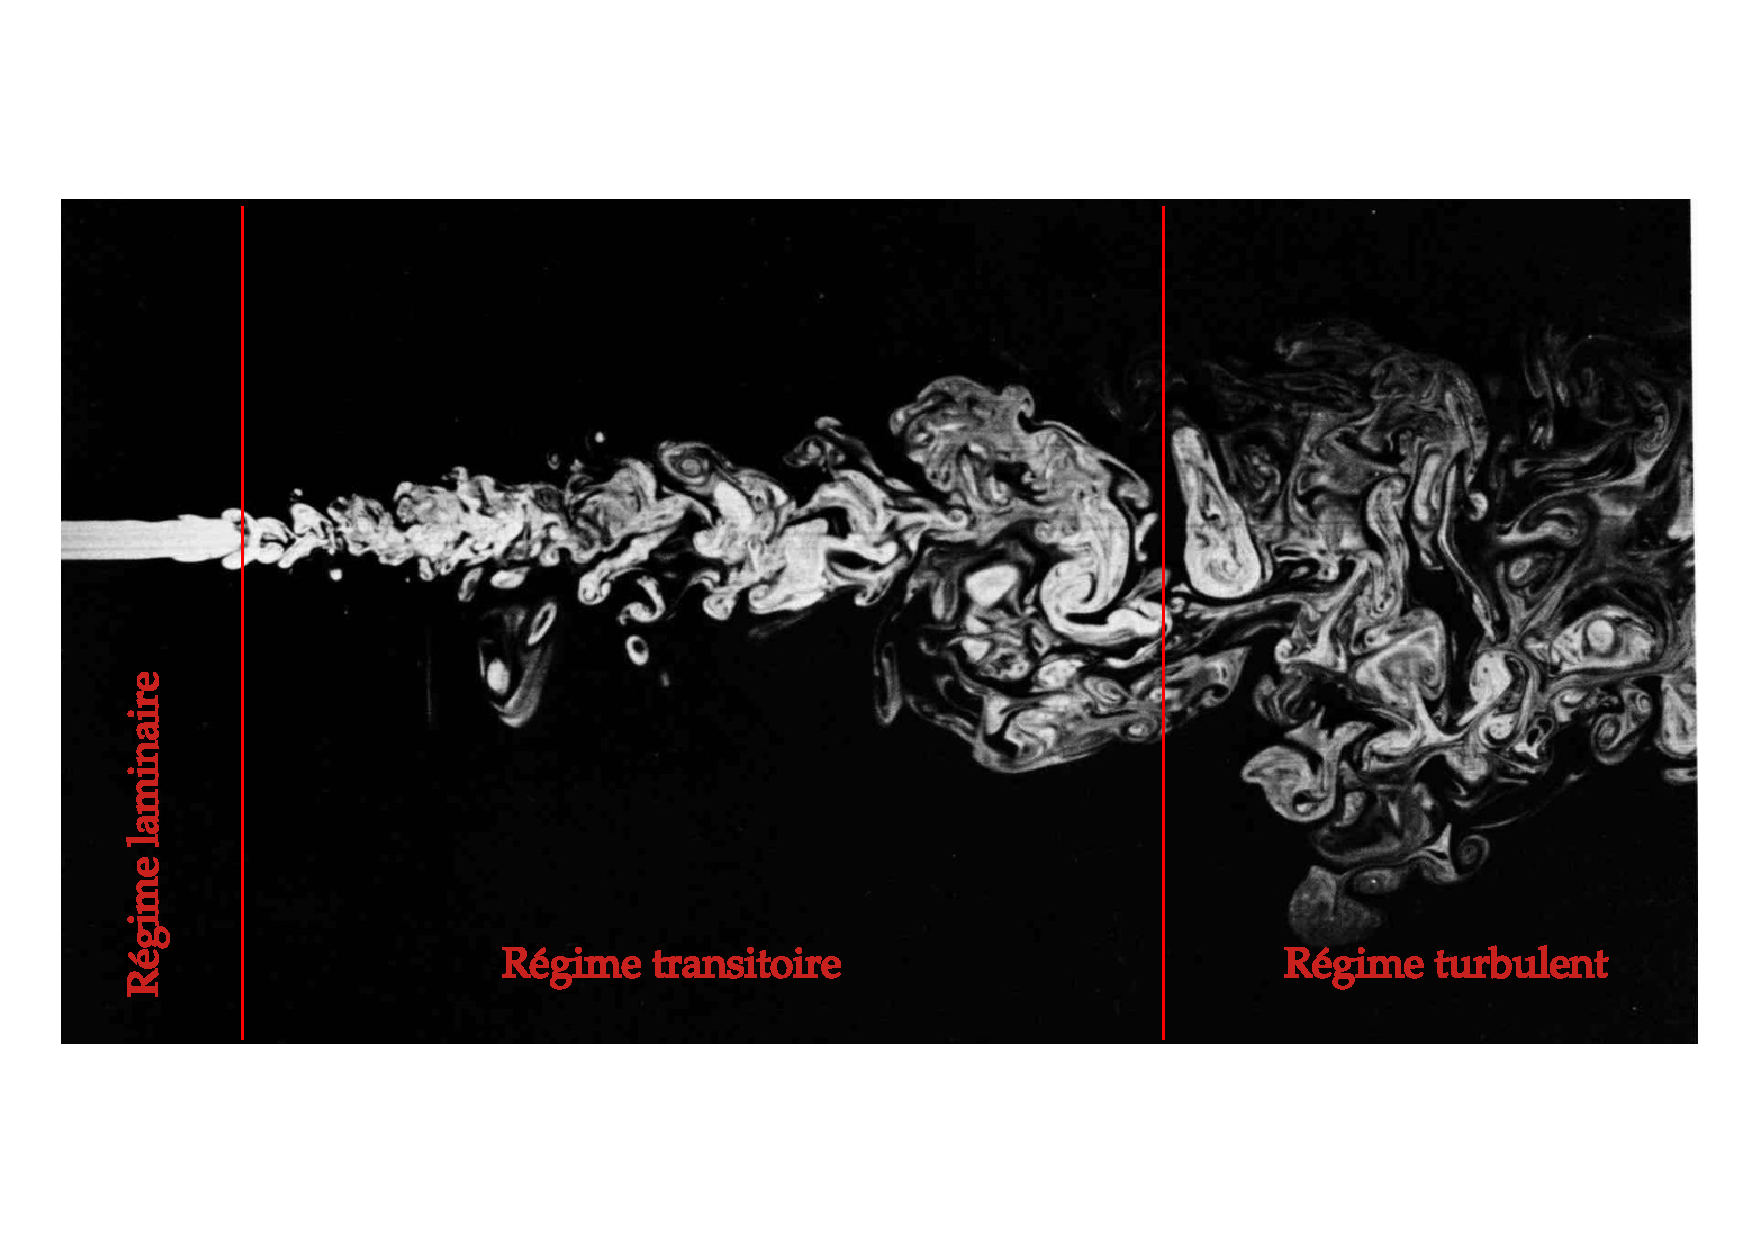
\includegraphics[width=\linewidth,trim=1cm 3cm 1cm 3cm, clip=true]{./Mainmatter/Part_0/images/turbul_Re}
 \caption{Injection d'un jet d'eau dans de l'eau observée par fluorescence laser et illustrant les différents régimes d'un écoulement : laminaire, transitoire et turbulent. [Crédits de l'image initiale : \cite{van_dyke_album_1982}.]}
 \label{fig:ecoulement}
 \end{figure}
 
 Dans le cadre hydrodynamique incompressible, l'écoulement n'est décrit que par les champs de vitesse et de pression, mais pour d'autres fluides, la description peut impliquer d'autres champs tels que le champ magnétique $\boldsymbol{B}$, le champ scalaire massique $\rho$, etc. On peut définir un nombre sans dimension similaire au nombre de Reynolds, rapport entre le terme non-linéaire convectif et le terme diffusif ou dissipatif impliqués dans l'évolution temporelle de ces champs. Dans le cas d'un champ magnétique, ce sera le nombre de Reynolds magnétique $R_m = \frac{VL}{\eta}$ avec $\eta$ la résistivité ou diffusivité magnétique. Pour des quantités thermodynamiques telles que la densité de masse ou la pression, on parlera plutôt de nombres de Péclet.
 
 Sur la \figref{fig:comp_turbul}, sont présentés des résultats d'une simulation turbulente \cacro{3D} qui sera introduite et utilisée dans la partie \ref{part_3}.
 \begin{figure}[!ht]
  \centering
 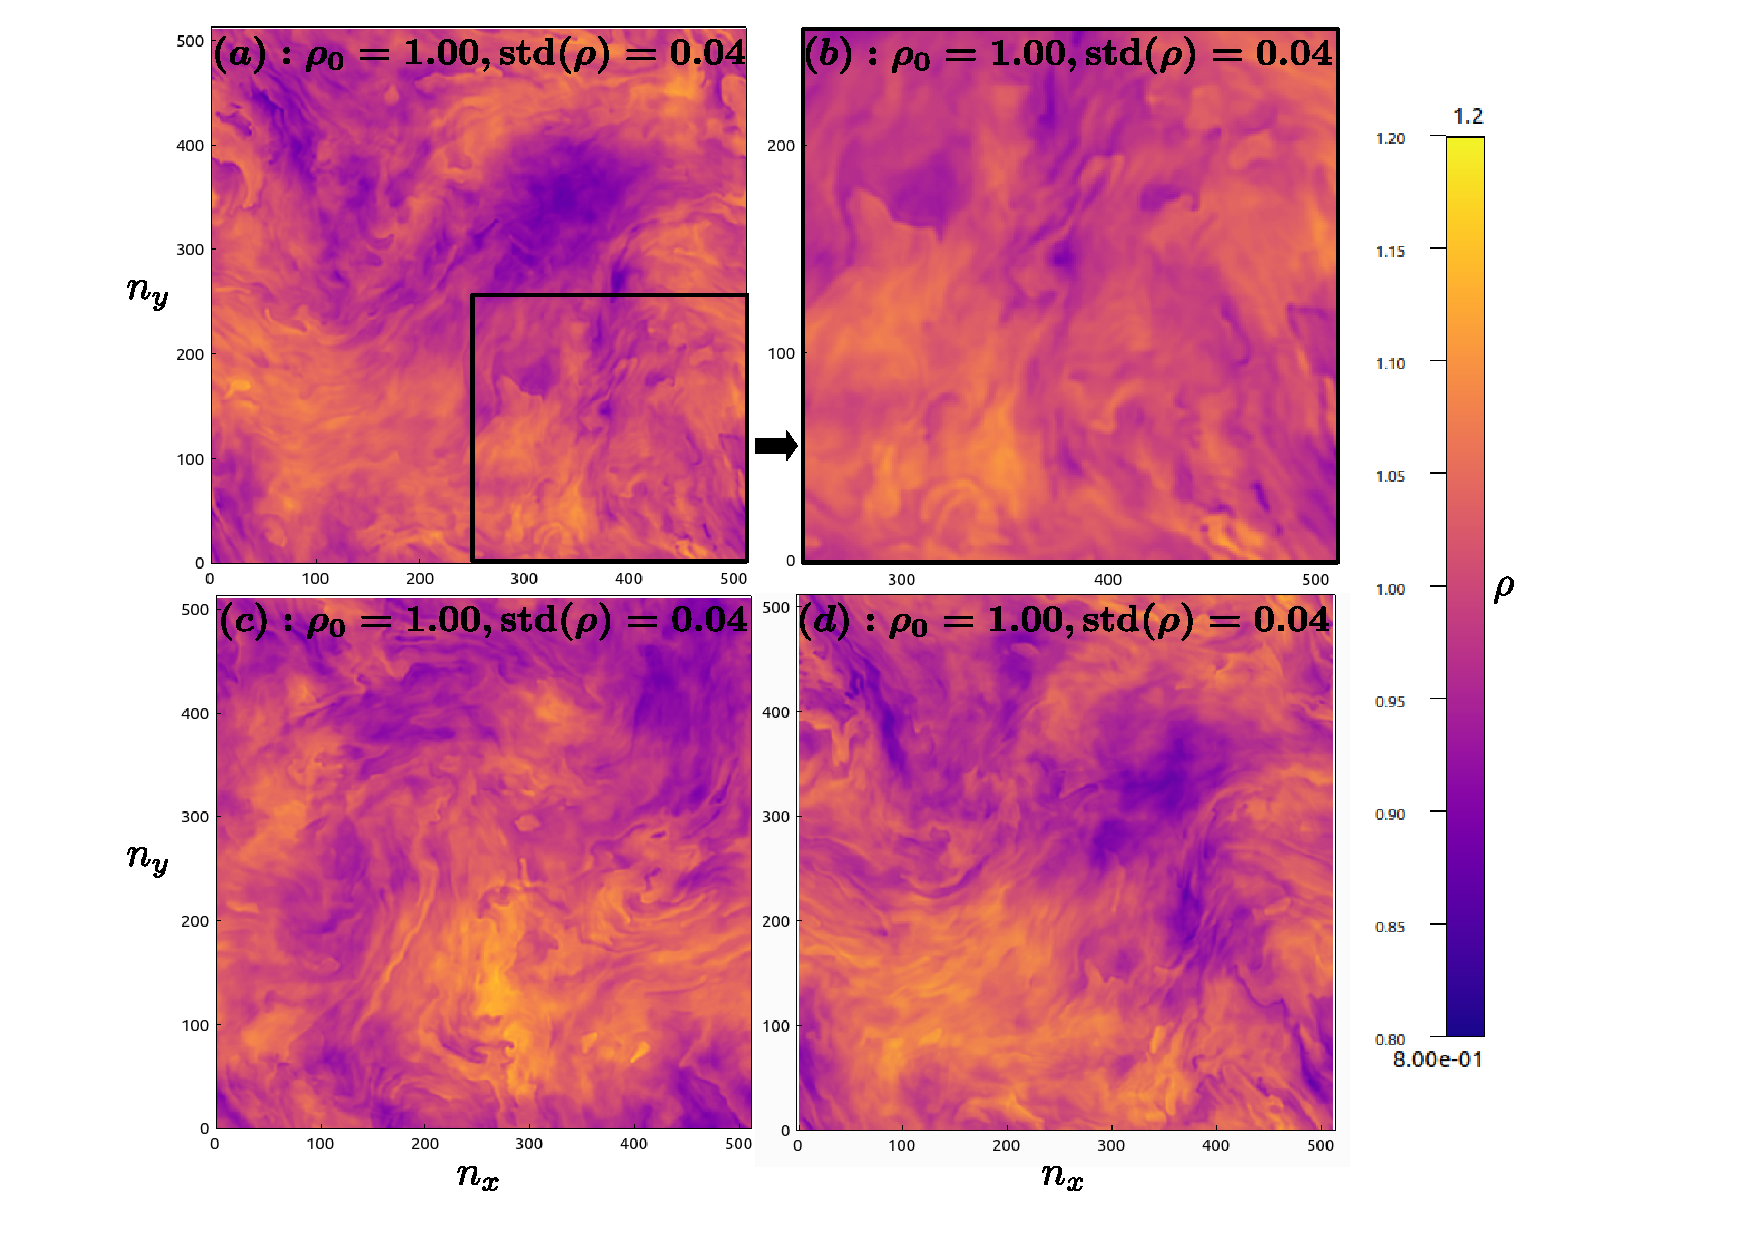
\includegraphics[width=0.8\linewidth,trim=2cm 0cm 4cm 0cm, clip=true]{./Mainmatter/Part_0/images/simu_panel_rho}
 \cprotect\caption{Résultats d'une simulation \cacro{3D} d'un plasma turbulent décrit par le modèle Hall-CGL. Le code de simulation sera introduit dans la partie \ref{part_3}. La quantité représentée est la densité $\rho$. Chaque image correspond à une coupe $x-y$ du cube de densité obtenu au temps $t$ (en unité de temps de la simulation). Les axes sont en position numérique (nombre de points dans chaque direction, comptés à partir d'une position $(0,0,0)$). (a) : $n_z=323$, $t=410$. (b) : zoom de (a). (c) : $n_z=638$, $t=410$. (d) : $n_z=323$, $t=408$. Pour chaque image, la moyenne spatiale, $\rho_0$, est de $\num{1.00}$ et l'écart-type, $\text{std}(\rho)$, de $\num{0.04}$.}
 \label{fig:comp_turbul}
 \end{figure}
 L'image (a) correspond à une coupe du cube de densité $\rho$ telle que $n_z=323$ obtenue au temps $t=410$. Si on la compare à l'image (c) (autre coupe du même cube telle que $n_z=638$), on remarque une certaine invariance spatiale statistique qui illustre la propriété d'homogénéité dite statistique d'un fluide turbulent. Si par contre, on la compare à l'image (d) (coupe $n_z=323$ obtenue à la date $t=408$), on retrouve similairement une certaine invariance temporelle qui vient illustrer la propriété de stationnarité statistique du fluide. Enfin, en comparant avec l'image (b) (zoom de l'image (a)), on observe ce qui semble être une loi d'échelle.
 
 Un écoulement ou un fluide turbulent serait donc caractérisé par
 \begin{itemize}
 \item une dominance des non-linéarités sur les contributions diffusives (grands nombres de Reynolds et de Péclet),
 \item des propriétés d'invariance (homogénéité, stationnarité) au sens statistique,
 \item une loi d'échelle.
 \end{itemize}
 Dans la section \ref{sec-012}, on va définir les notations et appellations liées aux notions mathématiques statistiques et dans la section \ref{sec-013}, on abordera un peu plus en détail la description de la turbulence à travers les échelles.
 
\section{Description statistique et notations pour l'étude d'un système turbulent}\label{sec-012}

Afin de garder la description du travail présenté dans ce mémoire accessible à tous, nous ne nous perdrons pas dans des définitions mathématiques complexes et exhaustives des notions, mais resterons sur des définitions exemplifiées et plus appliquées. 

Dans l'ensemble de ce mémoire, on se placera dans un cadre \cacro{3D}. Sauf quantités indéfinies, les grandeurs vectorielles seront notées en gras. Le système de représentation spatial sera génériquement cartésien $\mathbf{x} = (x,y,z)$, sauf mention contraire.

Soit une quantité indéfinie $X$ (densité, vitesse, pression, champ magnétique, etc.) caractérisant un fluide. La distribution de valeurs possibles pour $X$, ou distribution de probabilité de $X$, notée $\mathcal{P}_X$, peut être obtenue en considérant différents points de vue :
\begin{itemize}
    \item PV1 : décrire le fluide comme un ensemble souvent discret, par exemple de $N$ particules (atomes, molécules, etc.) associées individuellement à une valeur de la quantité $X$, notée $X_n$ avec $n \in [1;N]$,
    \item PV2 : regarder l'espace occupé par le fluide : un volume continu $V$ ou un nombre de points d'emplacement $\mathbf{x}$. La quantité $X$ sera alors évaluée en chacun d'eux et notée $X(\mathbf{x})$, 
    \item PV3 : ne considérer qu'une particule ou qu'un point, regarder les valeurs de $X$ au fil du temps sur une période $T$, et les noter $X(t)$. 
\end{itemize}
Ces différents points de vue ne sont pas forcément équivalents. Par exemple, si l'on regarde plusieurs types de particules et que les valeurs de $X$ dépendent de leur nature, ne regarder qu'une particule au fil du temps ne sera pas représentatif du système. Par la suite, on utilisera les représentations PV2 et PV3.  

Pour caractériser la distribution de probabilité de $X$, on peut utiliser divers outils statistiques. L'un d'eux est la moyenne (moment d'ordre 0), une opération linéaire que l'on va noter $\left< X \right>$ et qui est définie en fonction des points de vue :
\begin{itemize}
    \item PV1 : $\left<X\right>_{N} = \frac{1}{N} \sum_{n=1}^N X_n$, est la moyenne d'ensemble définie de manière discrète.
    \item PV2 : $\left<X\right>_{V} = \frac{1}{V} \int_V X(\mathbf{x}) \mathcal{P}_X d\mathbf{x}$, est la définition continue de la moyenne spatiale. $\left<X\right>_V$ est indépendante de la position locale $\mathbf{x}$. Dans le cas discret, en considérant un échantillonnage spatial, c'est-à-dire $N_V$ points dans le volume $V$, et en notant $X_p$ la valeur de $X$ au point $p$, $\left<X\right>_{V} = \frac{1}{N_V} \sum_{p=1}^{N_V} X_p$. 
    \item PV3 : $\left<X\right>_{T} = \frac{1}{T} \int_0^T X(t) \mathcal{P}_X dt$, est la définition continue de la moyenne temporelle. $\left<X\right>_T$ est indépendante de l'instant $t$. Une moyenne discrète peut aussi être définie en considérant un échantillonnage temporel.
\end{itemize}
Si $\left<X\right>_{N} = \left<X\right>_{V} = \left<X\right>_{T}$ est vérifiée, on peut supposer une équivalence statistique des différents points de vue. Le système sera alors ergodique. 

On peut définir plus rigoureusement les propriétés d'homogénéité et de stationnarité statistiques à l'aide de $\mathcal{P}_X$ : 
\begin{itemize}
    \item \textbf{\emph{homogénéité statistique}} : soient deux échantillons représentatifs du système et définis relativement à deux positions indépendantes l'une de l'autre $\mathbf{x}$ et $\mathbf{x'}$ alors  $\mathcal{P}_X(\mathbf{x}) = \mathcal{P}_X(\mathbf{x'}) = \mathcal{P}_X$, ce qui implique pour la moyenne $\left<X(\mathbf{x})\right> = \left<X(\mathbf{x'})\right> = \left<X\right>$,
    \item \textbf{\emph{stationnarité statistique}} : soient deux échantillons représentatifs du système et définis relativement à deux instants indépendants l'un de l'autre $t$ et $t'$ alors $\mathcal{P}_X(t) = \mathcal{P}_X(t') = \mathcal{P}_X$, ce qui implique pour la moyenne $\left<X(t)\right> = \left<X(t')\right> = \left<X\right>$.
\end{itemize}
Attention, cela ne signifie pas que localement, entre deux instants $t$ ou deux positions $\mathbf{x}$, $X$ sera constant. En pratique, dans des données d'observations ou de simulations, des échantillons dans lesquels ces hypothèses seraient parfaitement valides sont difficiles à obtenir. Des compromis devront donc être établis. 

Similairement aux définitions des propriétés d'homogénéité et de stationnarité statistiques, pour étudier un fluide turbulent, on doit relier le comportement statistique de deux échantillons ou plus, c'est-à-dire que l'on doit s'intéresser aux fluctuations, incréments de quantités et corrélations entre au moins deux échantillons. Ce lien peut s'exprimer en fonction de la distance temporelle ou spatiale entre ces échantillons, généralement appelée <<échelle>>. En 1941, Kolmogorov pose les bases d'une théorie permettant d'obtenir une telle relation : la théorie des lois exactes [\cite{frisch_turbulence_1995,kolmogorov_dissipation_1991,kolmogorov_local_1991}]. Cette théorie repose sur les hypothèses que nous avons illustrées dans la section \ref{sec-011} (dominance des effets non-linéaires, homogénéité et stationnarité statistiques) ainsi que sur une hypothèse plus spécifique de séparation d'échelle qui sera expliquée dans la section \ref{sec-013}.

Le travail décrit dans ce mémoire est basé sur cette théorie et implique les notations suivantes. On considèrera deux échantillons définis relativement à deux positions\footnote{Il est possible de corréler plus de deux points. Tout lecteur intéressé pourra se référer à [\cite{cho_simulations_2009}].}\footnote{Historiquement, les calculs sont effectués dans le cadre PV2. Il serait a priori possible de les transposer dans les cadres PV1 ou PV3, mais ce n'est pas l'objet de cette thèse.} indépendantes l'une de l'autre, $\mathbf{x}$ et $\mathbf{x'}$. La quantité indéfinie $X$ évaluée en $\mathbf{x'}$ sera notée $X'$ et celle évaluée en $\mathbf{x}$, $X$. L'échelle, notée $\boldsymbol{\ell}$, sera définie comme l'incrément de position : 
\begin{equation}
    \boldsymbol{\ell} = \delta \mathbf{x} = \mathbf{x'} - \mathbf{x} ,
\end{equation}
avec $\delta$ dénotant le caractère incrémental. Similairement l'incrément de la quantité indéfinie $X$ s'écrira : 
\begin{equation}
    \delta X = X' - X = X(\mathbf{x'}) - X(\mathbf{x})  .
\end{equation}

Le lien étudié entre les deux échantillons sera une fonction de corrélation spatiale entre deux quantités $X$ et $Y$ (ici indéfinies) qui s'obtient en considérant une quantité au point $\mathbf{x}$ et l'autre au point $\mathbf{x'}$, en les multipliant puis en moyennant. Afin de conserver une symétrie du rôle de $\mathbf{x}$ et $\mathbf{x'}$, on définira la fonction de corrélation telle que 
\begin{equation}
    \label{eq:def_correlation} \mathcal{R}_{XY} = \frac{1}{2} \left<X \cdot Y' + X' \cdot Y\right>,
\end{equation}
en notant $\cdot$ l'opération générique multiplicative. Entre deux vecteurs, cette opération pourrait être considérée comme un produit scalaire ou remplacée par un produit vectoriel noté $\times$. La fonction d'auto-corrélation est obtenue en considérant $X=Y$, c.-à-d. $\mathcal{R}_{XX} = \left<X \cdot X'\right>$. 
La moyenne $\left<\right>$ impliquée dans ces fonctions est la moyenne spatiale. $\mathcal{R}_{XY}$ sera donc indépendante de $\mathbf{x}$ et $\mathbf{x'}$ et ne dépendra que de $\boldsymbol{\ell}$ et a priori de $t$ si les quantités dépendent du temps. 

Par indépendance entre le temps et la position, la moyenne spatiale commute avec la dérivée temporelle : 
\begin{equation}
  \label{eq:prop_t}  \partial_t \left<X\right> = \left<\partial_t X\right> .
\end{equation}
On note  $\nabla_{\boldsymbol{\ell}} = \frac{\partial}{\partial \boldsymbol{\ell}}$ l'opérateur de dérivation spatiale dans l'espace global des échelles, $\nabla$ et $\nabla'$ les opérateurs de dérivation locaux respectivement en $\mathbf{x}$ et $\mathbf{x'}$. L'indépendance entre $\mathbf{x}$ et $\mathbf{x'}$, implique que :
\begin{equation}
  \label{eq:prop_x}    \nabla X' = 0,  \qquad \nabla' X = 0.
\end{equation}
Grâce à l'hypothèse d'homogénéité statistique, ces opérateurs dérivatifs vérifient\footnote{
Soient $A$, $B$ et $C$ des quantités indéfinies telles que $A(\boldsymbol{\ell}) = \left<B \cdot C'\right> = \left<B(\mathbf{x}) \cdot C(\mathbf{x'})\right>$  avec $\cdot$ une opération multiplicative quelconque et $\mathbf{x'} = \mathbf{x} + \boldsymbol{\ell}$. Alors, l'élément différentiel $d \boldsymbol{\ell} $ est égal à $d \mathbf{x'} - d \mathbf{x}$. 

À $\mathbf{x}$ fixé, $ d \boldsymbol{\ell} = d \mathbf{x'}$, alors
$\nabla_{\boldsymbol{\ell}} A(\boldsymbol{\ell}) = \left<\partial_{\boldsymbol{\ell}} (B \cdot  C')\right> = \left<\partial_{\mathbf{x'}} (B \cdot  C') \right> = \left<\nabla' (B \cdot  C')\right> $. D'où la relation entre les opérateurs :  $\nabla_{\boldsymbol{\ell}} \left<\right> = \left<\nabla'\right>$. Similairement, à $\mathbf{x'}$ fixé, $ d \boldsymbol{\ell} = - d \mathbf{x}$, d'où $\nabla_{\boldsymbol{\ell}} \left<\right> = - \left<\nabla\right>$.
}
\begin{equation}
   \label{eq:prop_l}   \nabla_{\boldsymbol{\ell}}\left<\right> = \left<\nabla' \right> = - \left<\nabla \right> .
\end{equation}

En turbulence, on utilise aussi communément la transformée de Fourier. Cette méthode permet de travailler dans un espace où la position est repérée par $\boldsymbol{k} \propto 1/\mathbf{x}$, et où toute quantité se retrouve décomposée en une série de \og modes \fg{} que l'on appelle un spectre. Dans le cas continu \cacro{3D}, on définit la transformée de Fourier de la quantité $X$ par 
\begin{equation}
    \tilde{X}(\boldsymbol{k}) = \frac{1}{(2\pi)^3} \iiint X(\mathbf{x}) e^{-i\boldsymbol{k} \cdot \mathbf{x}} d\mathbf{x}
\end{equation}
et la transformée inverse par 
\begin{equation}
    X(\mathbf{x}) = \iiint \tilde{X}(\boldsymbol{k}) e^{i\boldsymbol{k} \cdot \mathbf{x}} d\boldsymbol{k}.
\end{equation} 
On remarque qu'en termes de dimensions, si l'on note $[X]$ l'unité de $X$ et $L$ l'unité de longueur, $\tilde{X} \sim [X] L^3$.

Dans le cas continu \cacro{1D}, on aura similairement : 
\begin{equation}
    \tilde{X}(k) = \frac{1}{2\pi} \int X(x) e^{-ikx} dx , \qquad 
    X(x) = \int \tilde{X}(k) e^{ikx} dk
\end{equation} 
et en termes de dimensions, $\tilde{X} \sim [X] L$.

Ces notations et hypothèses seront utilisées tout au long de ce mémoire. Pour se familiariser avec leur utilisation, une application de la théorie de Kolmogorov à un écoulement hydrodynamique incompressible décrit par les équations de Navier-Stockes \eqref{eq:navst_r} et \eqref{eq:navst_v} est donnée dans la section \ref{sec-013}. Cette application va nous servir à introduire la notion de loi d'échelle et l'hypothèse de séparation d'échelle.



 \section{Théorie de Kolmogorov et loi d'échelle}\label{sec-013}
 
 La démonstration de Kolmogorov de 1941 [version traduite :  \cite{kolmogorov_dissipation_1991,kolmogorov_local_1991}] a été réécrite à de multiples reprises sous différentes formes. D'autres versions sont données par \cite{monin_statistical_1975}, \cite{frisch_turbulence_1995}, \cite{antonia_analogy_1997}, et \cite{galtier_physique_2021}. 
 
Pour faciliter les étapes de calcul, on va réécrire l'équation de Navier-Stockes \eqref{eq:navst_v} grâce à l'hypothèse incompressible \eqref{eq:navst_r} et y ajouter un terme de forçage $\boldsymbol{f_c}$ : 
\begin{equation}
  \label{eq:navst_v2}  \partial_t \boldsymbol{v} = - \nabla \cdot (\boldsymbol{v} \boldsymbol{v}) -  \frac{1}{\rho_0} \nabla p + \nu \Delta \boldsymbol{v} + \boldsymbol{f_c} 
.\end{equation}

La démonstration se base sur la recherche d'une équation d'évolution temporelle pour la fonction d'auto-corrélation $\mathcal{R}_{\boldsymbol{v}\boldsymbol{v}} = \left<\boldsymbol{v} \cdot \boldsymbol{v'}\right>$. Pour l'obtenir, on dérive temporellement $\mathcal{R}_{\boldsymbol{v}\boldsymbol{v}}$ grâce à la propriété \eqref{eq:prop_t} (étape \eqref{eq:step_1}), on injecte l'équation de Navier-Stockes \eqref{eq:navst_v2} (étape \eqref{eq:step_2}) puis on applique les propriétés \eqref{eq:prop_x} et \eqref{eq:prop_l} pour extraire les opérateurs dérivatifs spatiaux de la moyenne spatiale (étape \eqref{eq:step_3}) : 
\begin{eqnarray}
    \partial_t \mathcal{R}_{\boldsymbol{v}\boldsymbol{v}} &=& \left<\boldsymbol{v} \cdot \partial_t \boldsymbol{v'} + \boldsymbol{v'} \cdot \partial_t \boldsymbol{v}\right> \label{eq:step_1} \\ 
    &=& - \left< \nabla' \cdot (\boldsymbol{v'} \boldsymbol{v'}) \cdot \boldsymbol{v}   +  \nabla \cdot (\boldsymbol{v} \boldsymbol{v})\cdot\boldsymbol{v'} \right> - \frac{1}{\rho_0} \left<\boldsymbol{v} \cdot \nabla' P' + \boldsymbol{v'} \cdot \nabla P\right>  \nonumber \\
    && + \nu \left<\boldsymbol{v} \cdot \Delta' \boldsymbol{v'} + \boldsymbol{v'} \cdot \Delta \boldsymbol{v}\right> + \left<\boldsymbol{v} \cdot \boldsymbol{f'_c} + \boldsymbol{v'} \cdot \boldsymbol{f_c}\right> \label{eq:step_2} \\  
    &=& \nabla_{\boldsymbol{\ell}} \cdot \left< - \boldsymbol{v} \cdot \boldsymbol{v'} \boldsymbol{v'} + \boldsymbol{v'} \cdot \boldsymbol{v} \boldsymbol{v}\right>  + \frac{1}{\rho_0} \nabla_{\boldsymbol{\ell}} \cdot \left< - P' \boldsymbol{v} + P \boldsymbol{v'}\right> \nonumber \\
    && + 2 \nu \Delta_{\boldsymbol{\ell}} \left<\boldsymbol{v} \cdot \boldsymbol{v'} \right>  + \left<\boldsymbol{v} \cdot \boldsymbol{f'_c} + \boldsymbol{v'} \cdot \boldsymbol{f_c}\right>  \label{eq:step_3}  
.\end{eqnarray}
Avec l'hypothèse incompressible et celle d'homogénéité statistique (propriétés \eqref{eq:prop_x} et \eqref{eq:prop_l}), 
\begin{eqnarray}
    \nabla_{\boldsymbol{\ell}} \cdot \left< - P' \boldsymbol{v} + P \boldsymbol{v'}\right> &=& 0, \\
    \nabla_{\boldsymbol{\ell}} \cdot \left< - \boldsymbol{v} \cdot \boldsymbol{v'} \boldsymbol{v'} + \boldsymbol{v'} \cdot \boldsymbol{v} \boldsymbol{v}\right> &=& \frac{1}{2} \nabla_{\boldsymbol{\ell}} \cdot \left< \delta \boldsymbol{v} \cdot \delta \boldsymbol{v} \delta \boldsymbol{v} \right>, \\
    \left<\boldsymbol{v} \cdot \boldsymbol{f'_c} + \boldsymbol{v'} \cdot \boldsymbol{f_c}\right> &=& \left<\boldsymbol{v} \cdot \left(\boldsymbol{f_c}\left(\mathbf{x}+\boldsymbol{\ell}\right) +  \boldsymbol{f_c}\left(\mathbf{x}-\boldsymbol{\ell}\right)\right)\right>
.\end{eqnarray}

D'où l'équation dite \cacro{KHM}: 
\begin{equation}
    - \frac{\rho_0}{2} \partial_t \mathcal{R}_{\boldsymbol{v}\boldsymbol{v}} + \nu \rho_0 \Delta_{\boldsymbol{\ell}} \mathcal{R}_{\boldsymbol{v}\boldsymbol{v}} + \frac{\rho_0}{2} \left<\boldsymbol{v} \cdot \left(\boldsymbol{f_c}\left(\mathbf{x}+\boldsymbol{\ell}\right) +  \boldsymbol{f_c}\left(\mathbf{x}-\boldsymbol{\ell}\right)\right)\right> = - \frac{\rho_0}{4} \nabla_{\boldsymbol{\ell}} \cdot \left<\delta \boldsymbol{v} \cdot \delta \boldsymbol{v} \delta \boldsymbol{v}\right> \label{eq:KHM_HD}  
.\end{equation} 

Schématiquement, on va la noter : 
\begin{equation}
    \label{eq:bal_KHM} -\partial_t \mathcal{R} + \varepsilon_{NL} + \varepsilon_{F} + \varepsilon_{D} = 0 .
\end{equation} 
\begin{itemize}
    \item $\mathcal{R} = \frac{\rho_0}{2} \mathcal{R}_{\boldsymbol{v}\boldsymbol{v}}$, la fonction de corrélation de densité d'énergie totale (ici cinétique). En $\boldsymbol{\ell} = 0$, elle est égale à la densité d'énergie totale moyenne $\left<\frac{\boldsymbol{v}^2}{2}\right>$ du système.
    \item $\varepsilon_{NL} = \frac{1}{4} \rho_0 \nabla_{\boldsymbol{\ell}} \cdot \left<\delta \boldsymbol{v} \cdot \delta \boldsymbol{v} \delta \boldsymbol{v}\right>$, le taux de cascade ou de transfert non-linéaire de l'énergie incrémentale $\frac{1}{4} \rho_0 \left<\delta \boldsymbol{v}^2\right>$ à travers les échelles, il s'annule en $\boldsymbol{\ell} = 0$.
    \item $\varepsilon_{F} = \frac{1}{2} \rho_0 \left<\boldsymbol{v} \cdot \left(\boldsymbol{f_c}\left(\mathbf{x}+\boldsymbol{\ell}\right) +  \boldsymbol{f_c}\left(\mathbf{x}-\boldsymbol{\ell}\right)\right)\right>$, le taux de forçage dépendant des échelles. En $\boldsymbol{\ell} = 0$, il est égal à la densité d'énergie moyenne injectée $\rho_0 \left<\boldsymbol{v} \cdot  \boldsymbol{f_c}\right>$ dans le système par le forçage.
    \item $\varepsilon_{D} = \rho_0 \nu \Delta_{\boldsymbol{\ell}} \mathcal{R}_{\boldsymbol{v}\boldsymbol{v}}$, le taux de dissipation dépendant des échelles. En $\boldsymbol{\ell} = 0$, il est égal à la densité d'énergie moyenne dissipée par viscosité $\rho_0 \nu \left<\Delta \boldsymbol{v}^2\right>$.
\end{itemize}

On remarque qu'en $\boldsymbol{\ell} = 0$, \eqref{eq:KHM_HD} devient l'équation d'énergie totale moyenne que l'on peut noter : 
\begin{equation}
     \label{eq:bal_KHM0} -  \partial_t \mathcal{R}(\boldsymbol{\ell} =0)  + \varepsilon_{D}(\boldsymbol{\ell} =0) +  \varepsilon_{F}(\boldsymbol{\ell} =0) = 0  
.\end{equation} 

L'hypothèse de stationnarité statistique vient annuler toute dérivée temporelle de quantités moyennées. Par conséquent, les équations \eqref{eq:bal_KHM} et \eqref{eq:bal_KHM0} deviennent :  
\begin{eqnarray}
    \label{eq:bal_eps}\varepsilon_{NL} + \varepsilon_{F} + \varepsilon_{D} &=& 0 ,\\
    \label{eq:bal_eps0} \varepsilon_{D}(\boldsymbol{\ell} =0) +  \varepsilon_{F}(\boldsymbol{\ell} =0) &=& 0
.\end{eqnarray}


Les démonstrations existantes divergent dans le traitement des taux $\varepsilon_{F}$ et $\varepsilon_{D}$ de l'équation \eqref{eq:bal_eps} car elles ne prennent pas forcément en compte $\varepsilon_{F}$. Mais, toutes utilisent une propriété fondamentale de la turbulence, la loi <<zéroième>>. Cette loi indique que, pour un nombre de Reynolds grand, lorsque $\nu$ tend vers 0, la densité d'énergie dissipée moyenne $\rho_0 \nu  \left<\Delta\boldsymbol{v}^2\right>$, qui correspond à  $\varepsilon_D$ évalué en $\boldsymbol{\ell} =0$, devient indépendante de $\nu$ et ne s'annule pas. Cette singularité est aussi appelée anomalie dissipative. Elle indique la présence d'une dissipation dans la limite $R_e \gg 1$. On va noter $-\varepsilon$ cette valeur particulière de  $\varepsilon_D$. On peut alors résumer cette loi comme suit : 
\begin{equation}
 \label{eq:zero}  \varepsilon_D  \xrightarrow[\nu \rightarrow 0]{} \left\{
    \begin{aligned}
    & 0 & \textrm{si $\boldsymbol{\ell} \neq 0$ } \\
& - \varepsilon &  \textrm{si $\boldsymbol{\ell} =0$ } 
\end{aligned}
\right. .
\end{equation}

Si l'on prend en compte le terme de forçage, il sera supposé actif aux grandes échelles, notées $\boldsymbol{\ell_F} $. Aux échelles $\boldsymbol{\ell} \ll \boldsymbol{\ell_F}$, on obtient\footnote{Une démonstration de cette approximation est donnée dans l'Annexe \ref{an:forc} pour un forçage de type distribution de Dirac dans l'espace de Fourier.} $\varepsilon_{F} = \varepsilon_{F}(\boldsymbol{\ell} =0)$.  Avec la relation \eqref{eq:bal_eps0} et la loi zéroième \eqref{eq:zero}, on obtient alors $\varepsilon_{F}(\boldsymbol{\ell} \ll \boldsymbol{\ell_F}) = \varepsilon$. Enfin, en se plaçant à des échelles différentes de $\boldsymbol{\ell} =0$, telles que $\varepsilon_{D}=0$, on obtient de \eqref{eq:bal_eps}, la loi exacte \cacro{K41} : 
 \begin{equation}
  \label{eq:led_kolm} \frac{\varepsilon}{\rho_0} = - \frac{1}{4} \nabla_{\boldsymbol{\ell}} \cdot \left<\delta \boldsymbol{v} \cdot \delta \boldsymbol{v} \delta \boldsymbol{v}\right>
 \end{equation}
 qui s'écrit schématiquement $\varepsilon=-\varepsilon_{NL}$. Dans ce mémoire, nous déterminerons et analyserons $\varepsilon_{NL}$ pour différents modèles. Si l'on ne prend pas en compte le terme de forçage, on peut construire la différence entre \eqref{eq:bal_KHM} et \eqref{eq:bal_KHM0} et, dans la limite des grands nombres de Reynolds et avec l'hypothèse de stationnarité statistique, on peut retrouver \eqref{eq:led_kolm} [\cite{antonia_analogy_1997}]. 
 
 Cette loi est valable dans une gamme d'échelle dite inertielle où le comportement du fluide est supposé complètement non-linéaire ($R_e \gg 1$ et $\nu \rightarrow 0$) et peu impacté par tout phénomène d'injection d'énergie. La cascade d'énergie s'y effectue donc à un taux $\varepsilon$ constant. L'ensemble des dernières hypothèses est résumé sous le nom \textbf{\emph{\og hypothèse de séparation d'échelle \fg{} : 
 il existe une gamme d'échelle dite inertielle où l'énergie cascade conservativement (pas de dissipation, $\nu \rightarrow 0$ et $\boldsymbol{\ell} \neq 0$, ni de forçage, $\boldsymbol{\ell} \ll \boldsymbol{\ell_F}$) à un taux $\varepsilon$ constant.}} 
 
 Une autre hypothèse, communément appliquée en hydrodynamique, a été prise en compte par Kolmogorov, celle d'isotropie statistique. Elle permet d'obtenir une forme intégrée de la loi exacte. L'isotropie statistique implique une invariance angulaire sphérique. $\varepsilon(\boldsymbol{\ell})$ ne dépendra alors que de $\ell = |\boldsymbol{\ell}|$. On peut alors intégrer sur une boule de rayon $\ell$ la loi \eqref{eq:led_kolm} sachant que, dans la zone inertielle, $\varepsilon$ est constant. Ainsi, en notant $v_{\ell} = \boldsymbol{v} \cdot \boldsymbol{\ell}$, on a : 
 \begin{equation}
   \label{eq:kolmogorov}  - \frac{4}{3} \frac{\varepsilon}{\rho_0} \ell = \left<|\delta \boldsymbol{v}|^2 \delta v_{\ell}\right>.
 \end{equation}
 
 Phénoménologiquement, par analyse dimensionnelle, la loi exacte \eqref{eq:kolmogorov} s'écrit $(\delta v)^3 \sim \ell$ d'où $E(\ell) \sim (\delta v)^2 \sim \ell^{2/3}$. En passant dans l'espace de Fourier, sachant que l'on se place dans un cas \cacro{1D}, on peut remplacer $\ell$ par $1/k$ et $E(\ell)$ par $k E(k)$. On obtient alors le spectre énergétique :
 \begin{equation}
     E(k) \sim k^{-5/3}.
 \end{equation} 
 D'où, en représentation logarithmique, $\log E(k) = -5/3 \log k + C $ avec $C$ une constante. Ainsi, la théorie de Kolmogorov nous permet de prédire, dans le cas isotrope, un spectre d'énergie cinétique, $E(k)$ de pente $-5/3$ en représentation logarithmique. Malgré son caractère phénoménologique, cette prédiction est très bien retrouvée sur plusieurs ordres de grandeurs, par exemple dans le cadre expérimental (voir  \figref{fig:spec_kolmo}). 
 \begin{figure}[]
  \centering
 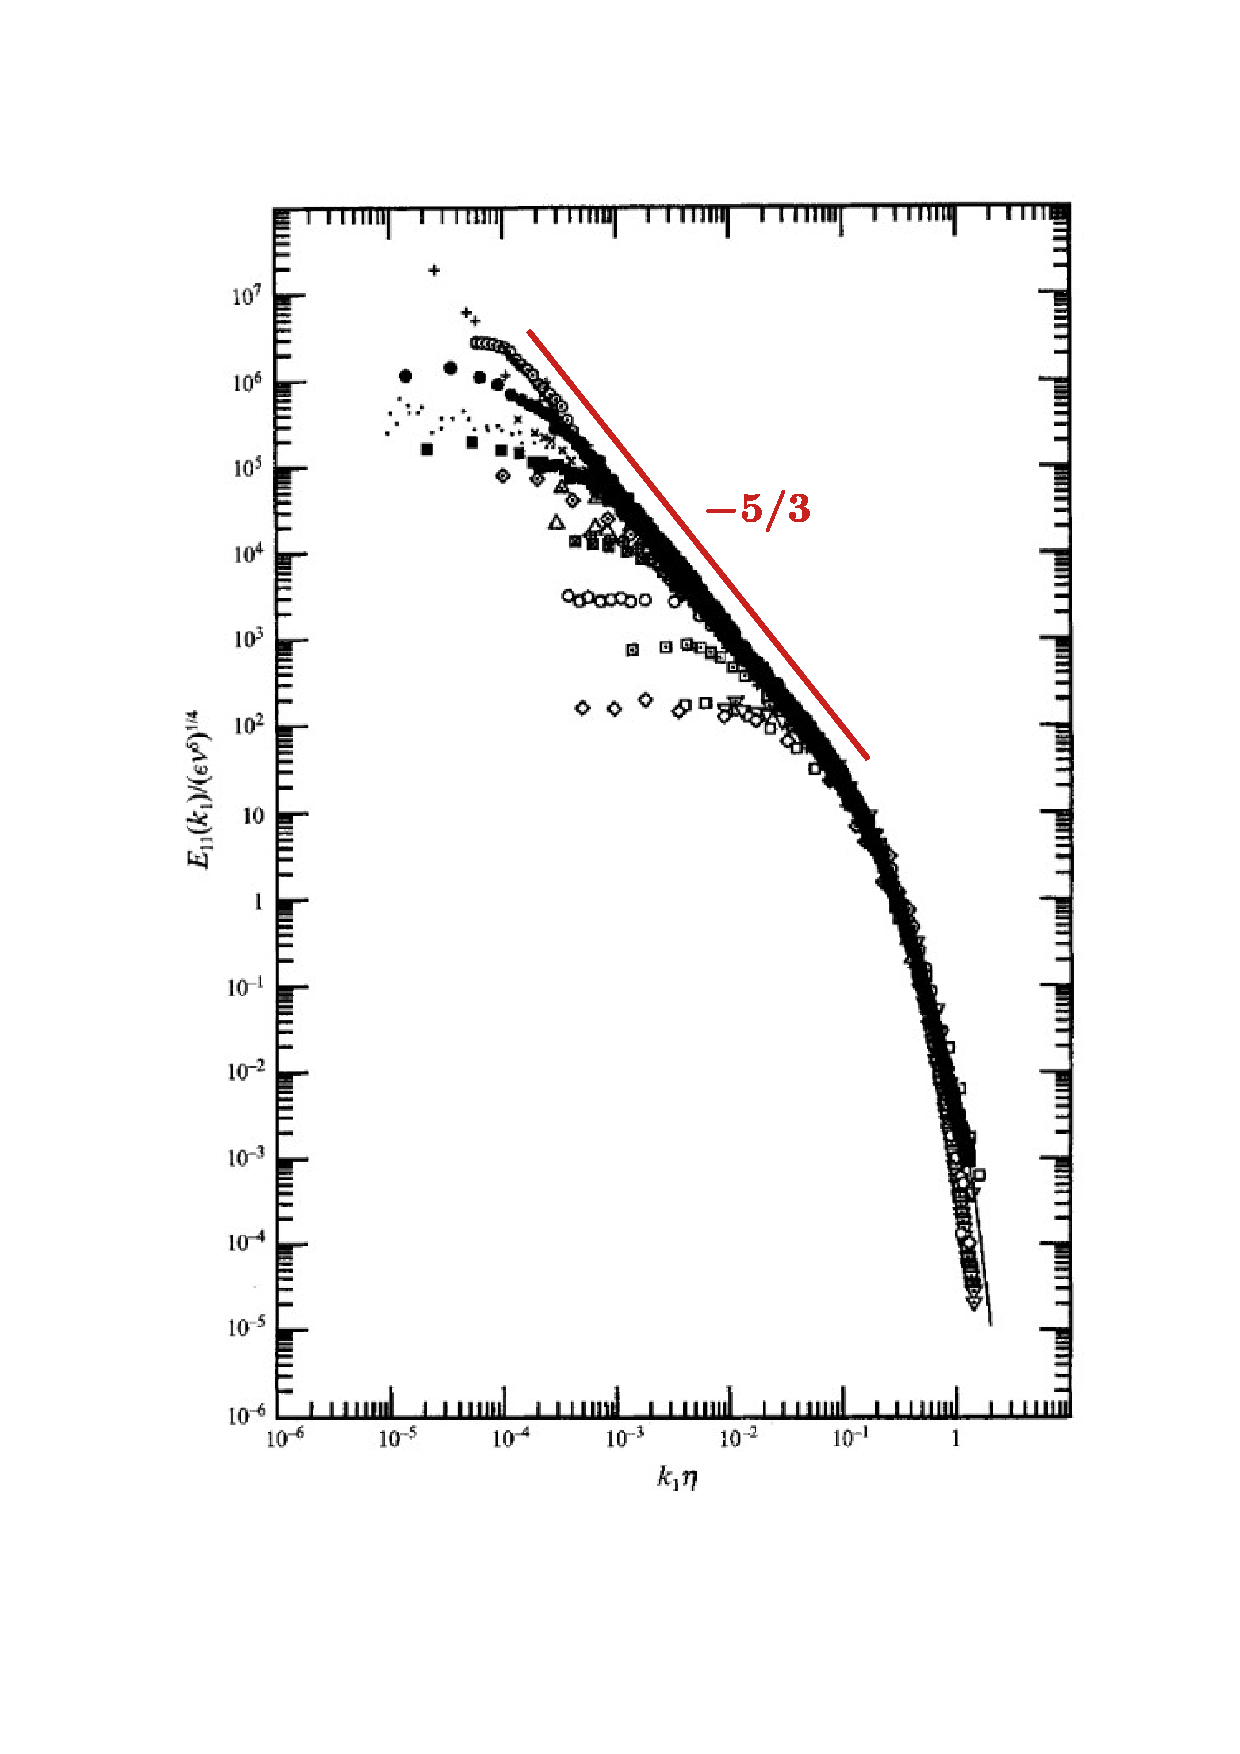
\includegraphics[width=0.8\linewidth,trim=1cm 4cm 1cm 3cm, clip=true]{./Mainmatter/Part_0/images/spectre_kolmogorov}
 \caption{Compilations de spectres obtenus dans diverses expériences de laboratoire. Tous ces spectres sont en accord avec la pente en $-5/3$ prédite grâce à la théorie de Kolmogorov. [Crédits : \cite{saddoughi_local_1994}.] }
 \label{fig:spec_kolmo}
 \end{figure}
 La forme $E(k) = C k^{\gamma}$ avec $C$ et $\gamma$ constants, qui s'écrit  en représentation logarithmique $\log E(k) = \gamma \log k + C $, est une loi d'échelle. Dans un système physique, une loi d'échelle ne va apparaître que sur une gamme d'échelle dédiée, limitée par la taille du système et l'émergence de phénomènes diffusifs à petites échelles, c'est à dire petits $\ell$ ou grands $k$. Ici, cette gamme est la zone de validité de la loi de Kolmogorov : la zone inertielle. 
 
 Cette définition spectrale de la zone inertielle turbulente, telle que le spectre affiche une loi d'échelle en $-5/3$, n'est pas aussi contraignante que la définition statistique via un taux $\varepsilon$ constant. En effet, le système vérifiera plus facilement la définition spectrale que la définition statistique car $E(k)$ est d'ordre 2 ($\propto (\delta v)^2$ et positif) alors que $\varepsilon$ est d'ordre 3 ($\propto (\delta v)^3$ et signé). Autrement dit, observer une pente $-5/3$ de type Kolmogorov ne sera pas forcément synonyme d'un régime de turbulence complètement développée définie par l'existence d'une zone inertielle telle que $\varepsilon$ constant. 
 
 \section{Synthèse des hypothèses de Kolmogorov et de la description de la cascade turbulente via des lois exactes}
 \label{synt-01}
 \fcolorbox{blue}{white}{\begin{minipage}[c]{\linewidth}
  \paragraph{Taux énergétiques échelles-dépendants : }
  \begin{itemize}
      \item Taux de cascade (transfert non linéaire entre les échelles) : $\varepsilon_{NL}(\boldsymbol{\ell})$,
      \item Taux d'injection (forçage) : $\varepsilon_{F}(\boldsymbol{\ell})$,
      \item Taux de dissipation : $\varepsilon_{D}(\boldsymbol{\ell})$.
  \end{itemize}
 
 \paragraph{Loi zéroième ou anomalie dissipative : } $\varepsilon_{D}(\boldsymbol{\ell}= 0) \xrightarrow[\nu \rightarrow 0]{} - \varepsilon \neq 0$. \\$\varepsilon$ correspond au taux de dissipation turbulent.
 
 \paragraph{Méthode d'obtention d'une loi exacte : }
 \begin{itemize}
     \item Dériver l'évolution temporelle d'une fonction de corrélation $\mathcal{R}$ entre deux points indépendants $\mathbf{x}$ et $\mathbf{x'}$ séparés de l'échelle $\boldsymbol{\ell}$, 
     \item Prendre en compte l'hypothèse d'homogénéité statistique, \\ $\Rightarrow$ Loi exacte de type \cacro{KHM}
     \item Appliquer les hypothèses de Kolmogorov de stationarité statistique et séparation d'échelle $\Rightarrow$ Loi exacte de type \cacro{K41}
 \end{itemize}
 
 \paragraph{Propriété liée à l'hypothèse d'homogénéité statistique : } 
 \begin{equation*}
     \Rightarrow \nabla_{\boldsymbol{\ell}}\left<.\right> = \left<\nabla' .\right> = - \left<\nabla . \right>
 \end{equation*}
 
 \paragraph{Propriété liée à l'hypothèse de stationnarité statistique : } $\Rightarrow \partial_t \left<.\right> = 0$.
 
 \paragraph{Hypothèse de séparation d'échelle : } Séparation des gammes d'échelles d'injection/forçage, de cascade/inertielles, et de dissipation/chauffage permise par la loi zéroième.
 \begin{equation*}
 \Rightarrow  \varepsilon_{NL}(0 \ll \boldsymbol{\ell} \ll \boldsymbol{\ell_F} ) = - \varepsilon_{F}(\boldsymbol{\ell} \ll \boldsymbol{\ell_F} ) = \varepsilon_{D}(\boldsymbol{\ell}=0) = - \varepsilon
 \end{equation*}
 
 \paragraph{Loi exacte de type KHM : } $\partial_t \mathcal{R} = \varepsilon_{NL} + \varepsilon_{F} + \varepsilon_{D}$
 
 \paragraph{Loi exacte de type K41 : } $\varepsilon = -\varepsilon_{NL}$
\end{minipage}}

\chapter{Qu'est-ce qu'un plasma ? De l'exemple du vent solaire à la problématique d'étude}
\renewcommand\partie{\Partie\ Chapitre \thechapter}
\label{ch-02}

%\medskip
\minitoc  

\bigskip

Dans le Chapitre \ref{ch-01}, nous avons défini de manière hydrodynamique (HD) ce qu'est la turbulence grâce à la théorie des lois exactes de Kolmogorov. Ce sera le seul chapitre placé dans le domaine hydrodynamique. Dans l'univers visible (ou baryonique), la matière est majoritairement sous forme de plasma que l'on ne peut décrire par les équations de Navier-Stockes incompressibles seules. On s'intéressera donc à la turbulence dans un plasma. 

Ici, nous allons définir ce qu'est un plasma et comment le décrire, puis nous aborderons les questions ouvertes, motivations des travaux décrits dans ce mémoire. 

\section{Les plasmas, état de la matière} \label{sec-021}

La matière peut être décrite comme des poupées russes constituées de particules de tailles diverses, allant des atomes et molécules aux quarks en passant par les protons et les électrons qui sont des particules chargées positivement et négativement. Elle peut aussi être décrite en fonction de son état : solide, liquide, gaz et plasma. 

Les états solide, liquide et gaz sont les états les plus reconnus dans notre quotidien. Ils sont généralement constitués de molécules ou d'atomes neutres ne portant pas de charge électrique. Pourtant, ces états sont des exceptions dans l'univers, où la matière est majoritairement à l'état de plasma : les atomes y sont dissociés en particules chargées, ions, protons et électrons. Ces particules induisent un champ électromagnétique s'il n'y en a pas originellement. Le plasma sera entretenu par les interactions entre les champs électrique et magnétique et les particules. \textbf{\emph{Un plasma est donc un milieu constitué de particules chargées et de champs électrique et magnétique en étroite interaction.}}

On peut aussi en reconnaître dans notre quotidien, le plus souvent ils brillent ! Par exemple, les éclairs, les aurores, les flammes, les néons, les étoiles et les nébuleuses. Ils forment finalement la grande majorité de la matière présente dans l'univers, du centre des planètes au milieu intergalactique. Pour les étudier, on a deux possibilités : les créer en laboratoire ou s'immerger dedans. Dans le deuxième cas, peu sont réellement accessibles, beaucoup étant trop furtif (les éclairs), trop lointains (les nébuleuses) ou trop extrêmes (le soleil) pour y envoyer des appareils de mesure. Parmi les plasmas naturels accessibles, l'espace interplanétaire est roi. Véritable laboratoire [\cite{bruno_solar_2005}], on y envoie régulièrement des sondes et satellites. La dernière sonde en date est \ac{JUICE} lancée le 14 avril 2023 en direction du système lunaire de Jupiter. 

Dans l'espace interplanétaire, on trouve différents types de plasmas. Si l'on décolle de la surface d'une planète telle que la Terre, on commencera par traverser l'atmosphère constituée de gaz neutre. Puis, on atteindra l'ionosphère, un plasma d'ions lourds et impactés par le champ magnétique planétaire. En s'écartant un peu plus, on s'immergera dans la magnétosphère constituée d'ions légers (principalement des protons) et d'électrons, toujours sous l'influence du champ planétaire. En partant du Soleil, on peut aussi définir différentes couches, la chromosphère, une couche fine gazeuse, puis la couronne solaire, un plasma s'étendant sur une quinzaine de rayons solaires et enfin l'héliosphère dans lequel baignent les planètes. Le Soleil y éjecte continuellement un plasma : le vent solaire.
Le mouvement des planètes dans le vent solaire vient former un arc de choc les précédant. Entre cet arc et la magnétosphère, le vent solaire est choqué. Cette région, dominée par le champ magnétique interplanétaire, est la magnétogaine. La \figref{fig:régions} illustre quelques-unes de ces différentes régions. D'autres régions plus spécifiques existent, mais on se contentera de ce niveau de description, le vent solaire étant notre principal objet d'étude. 
\begin{figure}[!ht]
 \centering
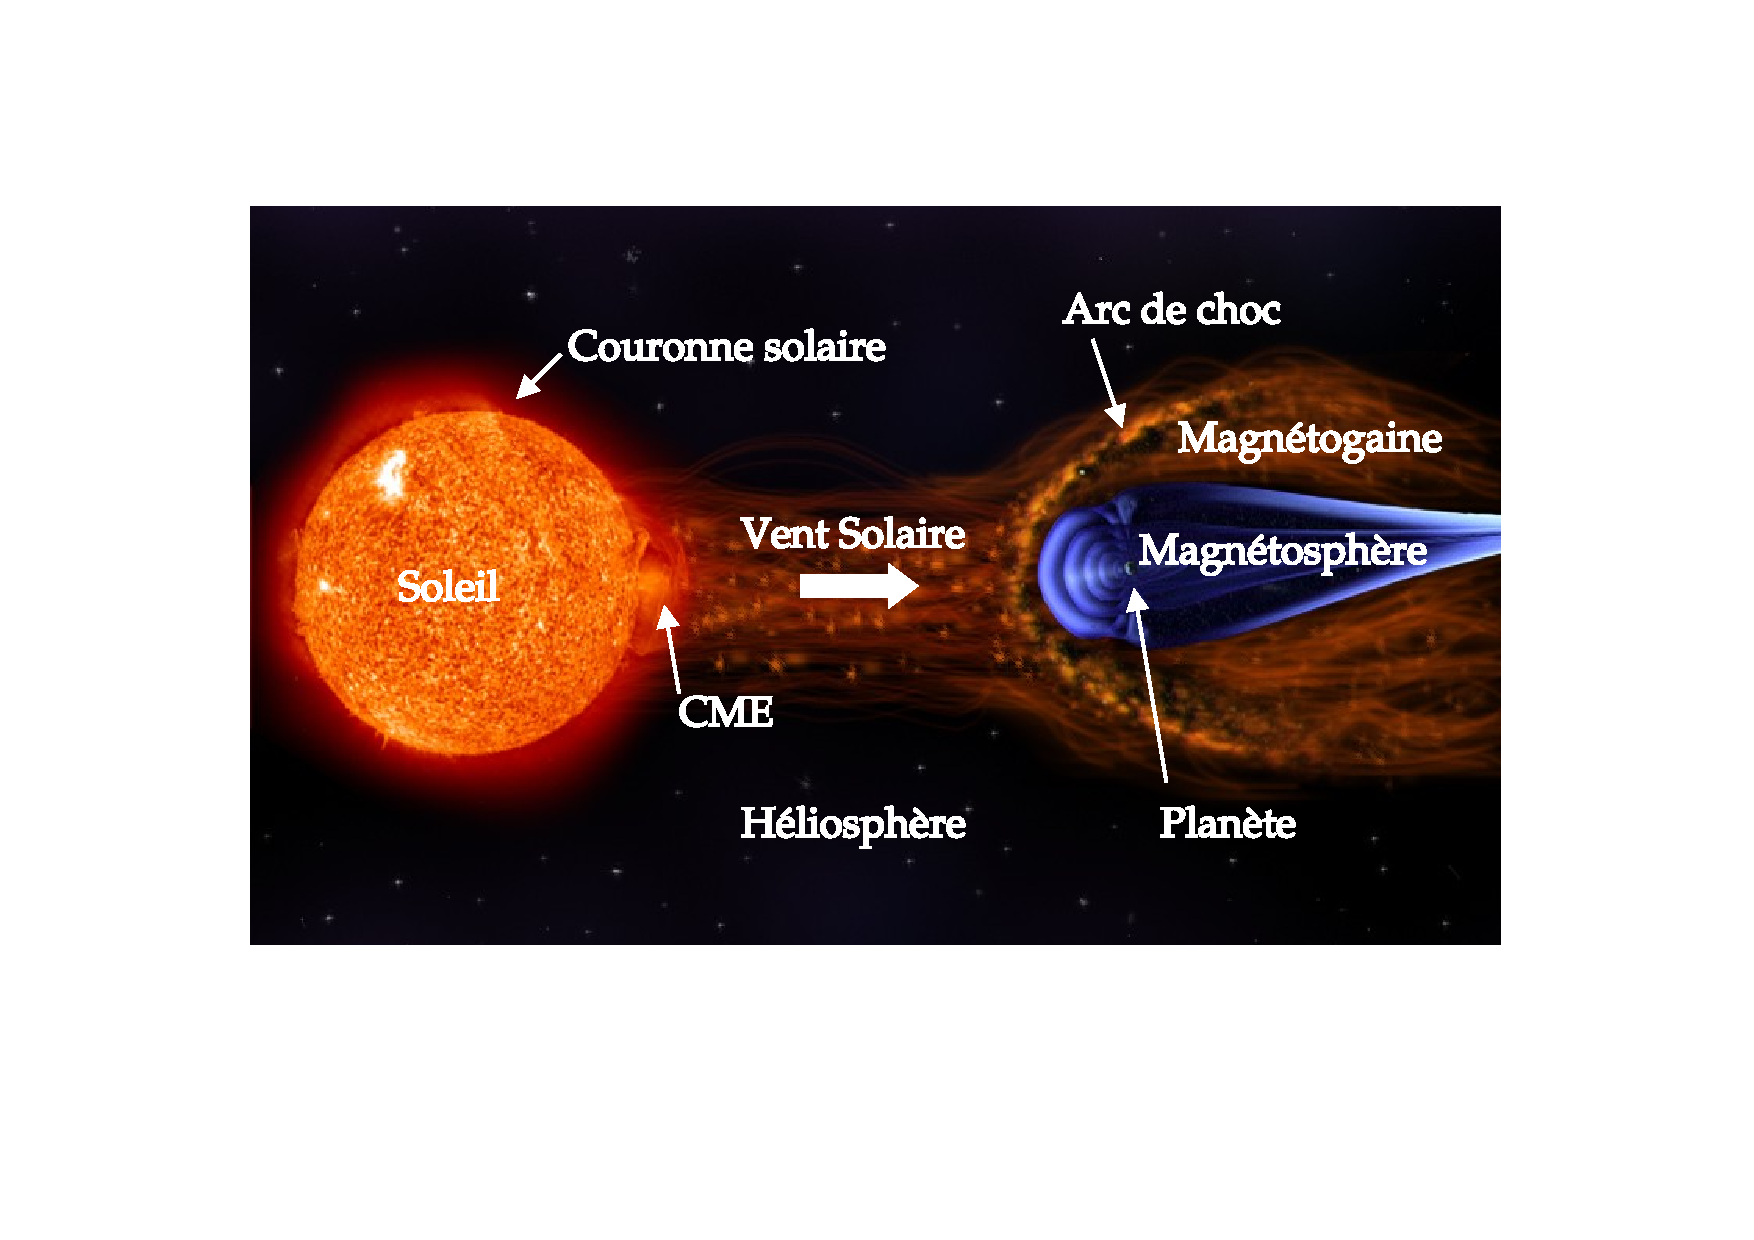
\includegraphics[width=\linewidth,trim=4cm 5cm 4cm 4cm, clip=true]{./Part_0/images/schemes_heliosphere}
\cprotect\caption{Exemples de plasmas spatiaux. \acs{CME} signifie éjections de masse coronale. Crédits de l'image initiale : Institut royal d'Aéronomie Spatiale de Belgique (page web \verb|www.aeronomie.be|).}
\label{fig:régions}
\end{figure}
Le vent solaire est par exemple traversé par \ac{PSP} en orbite autour du Soleil, cette mission lancée par l'agence spatiale américaine \acs{NASA} en 2018 s'approche petit à petit du Soleil afin de <<toucher>> la couronne. La mission \ac{MMS} en orbite autour de la Terre explore le vent solaire, la magnétogaine et la magnétosphère. Nous reparlerons plus en détail de ces deux missions dans le Chapitre \ref{ch-14}. 

\section{Le vent solaire, source de questions ouvertes et problématique d'étude} \label{sec-022}

Le vent solaire est un plasma extrêmement dilué, peu collisionnel et turbulent, constitué essentiellement d'ions légers ou protons (hydrogène, hélium chargés) et d'électrons interagissant avec le champ magnétique du Soleil. En fonction de l'activité cyclique et des latitudes du Soleil, il peut être rapide ($v_{SW} \sim \SI{800}{km/s}$) ou lent ($v_{SW} \sim \SI{400}{km/s}$) et parcouru par des structures à grandes échelles telles que les \ac{CME}. Les missions Voyager 1 et 2, lancées en 1977 vers les confins de l'héliosphère par la NASA, ont permis de tracer les profils de température, champ magnétique, vitesse etc. en fonction de la distance au Soleil [\cite{richardson_radial_1995}]. Ces profils ont donné lieu à diverses modélisations et à des problèmes ouverts encore aujourd'hui. 

\begin{figure}[!ht]
 \centering
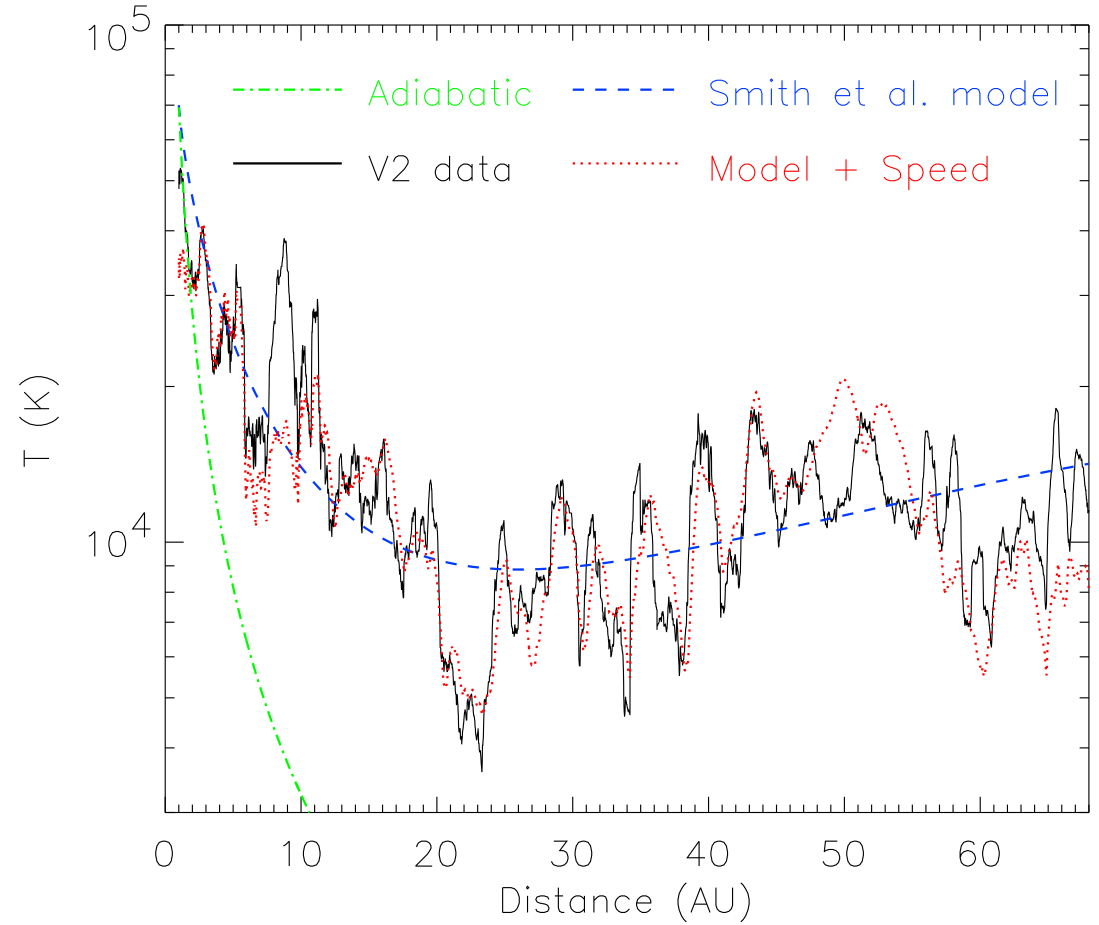
\includegraphics[width=0.8\linewidth,trim=0.5cm 0cm 0cm 0cm, clip=true]{./Part_0/images/heating_profil}
\cprotect\caption{Profil de température ionique en fonction de la distance au Soleil, observé avec les données de Voyager 2 (noir). Profil adiabatique (vert).  Crédits : [\cite{richardson_radial_2003}].}
\label{fig:profil}
\end{figure}
Sur la \figref{fig:profil} est donné l'exemple du profil de température. Du caractère peu collisionnel du vent solaire ont émergé, dans un premier temps, des prédictions d'une décroissance adiabatique du profil de température (courbe verte) [\cite{tu_mhd_1995}]. Comme on peut l'observer, la décroissance n'est pas aussi rapide que le modèle adiabatique. Des exemples de modélisations pour retrouver ce profil sont référencés par [\cite{richardson_radial_2003}]. Sur la \figref{fig:profil}, des résultats d'un modèle prenant en compte des ions dits <<pickups>> sont présentés en bleu et en rouge. Dans le cas rouge, est ajouté au modèle une dépendance linéaire entre la vitesse du vent solaire et la température. Le profil in-situ est ainsi plutôt bien retrouvé mais initialisé à partir de relevés de vitesse et température effectués autour de $\SI{1}{au}$ (unité astronomique dont l'étalon est la distance Soleil-Terre). Les ions pickups font en effet partie des sources du chauffage localisé du vent solaire mais ce chauffage aurait d'autres sources, comme l'explique \cite{david_energy_2022}. 
Avant $\SI{1}{au}$, il serait principalement dû aux fluctuations turbulentes, puis aux chocs interplanétaires venant accélérer ou ralentir le plasma, et enfin, après $\SI{20}{au}$, aux ions pickups provenant du milieu interstellaire. Le chauffage dû aux fluctuations turbulentes est souvent mis en compétition avec un chauffage induit par les processus de reconnexion des lignes de champ magnétique [\cite{matthaeus_who_2011,cranmer_role_2015}]. Ces deux phénomènes sont souvent liés [\cite{sundkvist_dissipation_2007,retino_situ_2007,servidio_magnetic_2011,chasapis_thin_2015,manzini_subion-scale_2023}].  

Dans ces travaux, on s'intéresse au chauffage turbulent [\cite{tu_mhd_1995,kiyani_dissipation_2015}] prédominant à partir de quelques rayons solaires jusqu'à $\SI{2}{au}$. Une définition thermodynamique de ce chauffage sera donnée dans le Chapitre \ref{ch-12}. Ce problème sera abordé à travers la cascade turbulente définie dans le Chapitre \ref{ch-01} et décrite avec une théorie des lois exactes, héritage de la théorie de Kolmogorov. Elle permet un transfert d'énergie des grandes échelles d'injection, à travers les échelles dites fluides et vers les petites échelles (échelles dites cinétiques) où les processus cinétiques dissipatifs peuvent intervenir afin de chauffer les ions et les électrons. 

Ce transfert peut être illustré à partir des spectres d'énergie magnétique comme celui de la \figref{fig:spectre_SW} compilé grâce aux relevés de champ magnétique effectués in-situ par les missions \ac{ACE} et \acs{CLUSTER} en orbite autour de la Terre.  Sur cette figure, on retrouve en fonction de la fréquence temporelle $f$ une pente de type Kolmogorov en $-5/3 \simeq -1.7$. L'hypothèse de Taylor permet de relier le vecteur d'onde $\boldsymbol{k}$ introduit dans le Chapitre \ref{ch-01}, à la fréquence temporelle $f$ accessible dans les relevés in-situ, grâce à la vitesse du vent ($\boldsymbol{v}_{SW}$) : $2 \pi f \sim \boldsymbol{v}_{SW} \cdot \boldsymbol{k}$.
Cette pente indique donc les échelles inertielles et la présence de turbulence dans le plasma d'après la définition spectrale de la zone inertielle donnée dans le Chapitre \ref{ch-01} et transposée à l'énergie magnétique. 
À plus hautes fréquences, cette zone inertielle s'achève par une rupture de pente autour de la fréquence associée à une longueur caractéristique ionique (la longueur d'inertie ($d_i$) ou le rayon de Larmor ($\rho_{Li}$) noté sur la figure $\rho_i$). 
À partir de cette échelle, des effets cinétiques ioniques commencent donc à être visibles. Ensuite, le spectre semble se stabiliser autour d'un nouveau régime a priori dispersif, avec une pente proche de $-2.6$, avant d'atteindre la zone d'influence des électrons autour de la fréquence associée à une longueur caractéristique électronique ($d_e$ ou $\rho_{Le}$, noté sur la figure $\rho_e$). Les phénomènes d'origine cinétique impliqués dans la zone de transition et les zones qui s'ensuivent ne sont pas encore complètement compris, tout comme leurs impacts sur les régimes turbulents (voir par exemple \cite{alexandrova_solar_2013} et \cite{sahraoui_magnetohydrodynamic_2020}). 
\begin{figure}[!ht]
 \centering
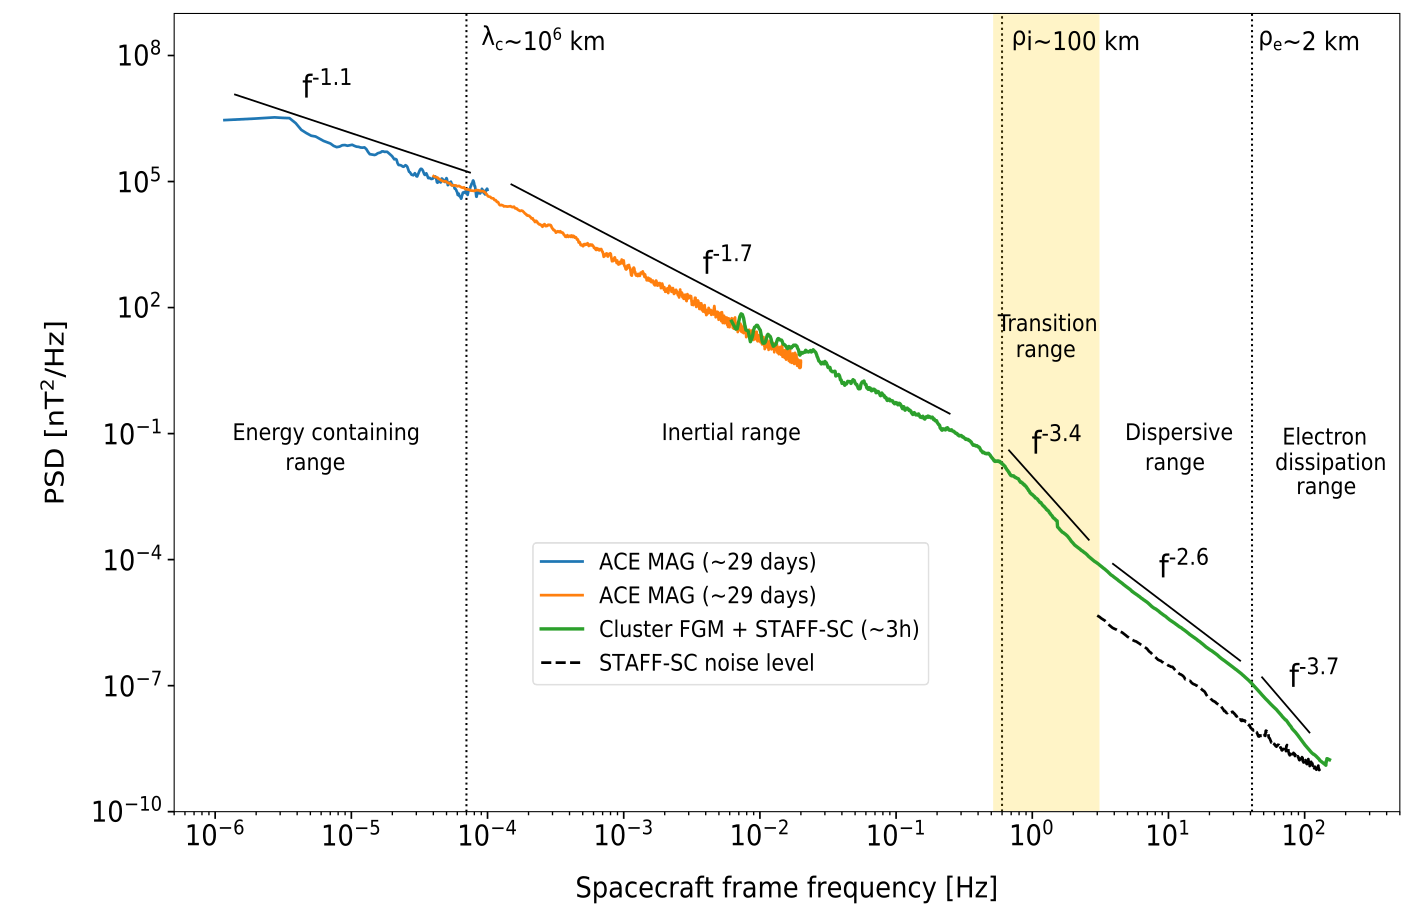
\includegraphics[width=\linewidth,trim=0.5cm 0cm 0cm 0cm, clip=true]{./Part_0/images/spectre_SW}
\cprotect\caption{Spectre d'énergie magnétique du vent solaire obtenu à partir des missions ACE et Cluster. Ce spectre peut être découpé en cinq régions grâce aux ruptures de pentes. Pente en $-1.1$ : Réservoir d'énergie. $\lambda_c$ : longueur de corrélation. Pente en $-1.7$ : Zone inertielle. $\rho_i$ : rayon de Larmor ionique. Pente en $-3.4$ : Zone de transition. Pente en $-2.6$ : Échelles dispersives. $\rho_e$ : rayon de Larmor électronique. Pente en $-3.7$ : Échelles de dissipation électronique. Crédits : [\cite{sahraoui_magnetohydrodynamic_2020}].}
\label{fig:spectre_SW}
\end{figure}

Parmi ces questions ouvertes dans l'étude de la turbulence compressible pour le chauffage du vent solaire, on s'attaquera aux effets conjoints du manque de collision et du champ magnétique sur la cascade. Ces deux propriétés induisent une anisotropie de la fonction de distribution de vitesse des particules, menant à un tenseur de pression anisotrope. Cette anisotropie de pression peut induire des instabilités dans le système [\cite{parker_dynamical_1958,berezin_firehose_1976,hall_firehose_1981,southwood_mirror_1993,gary_proton_1976,hunana_introductory_2019}]. 

La cascade turbulente d'énergie a été largement étudiée dans le cas incompressible depuis le début du siècle et l'extension de la théorie des lois exactes de Kolmogorov au modèle magnétohydrodynamique incompressible par \cite{politano_von_1998} et \cite{politano_dynamical_1998}. Les études sur l'effet de la compression sur la cascade sont quant à elles plus récentes et leur cadre souvent limité par l'hypothèse thermodynamique isotherme [\cite{marino_scaling_2023}]. Dans le Chapitre \ref{ch-11}, nous reprendrons quelques résultats incompressibles avant d'apporter dans la Partie \ref{part_1} une première extension du cadre d'étude de la cascade turbulente à des plasmas compressibles, en centrant la problématique sur l'effet de différentes descriptions thermodynamiques utilisées pour définir la pression. Dans la Partie \ref{part_2}, nous élargirons le cadre de la théorie des lois exactes en prenant en compte l'anisotropie de pression. Dans la Partie \ref{part_3}, nous appliquerons la théorie analytique ainsi élargie à des simulations tridimensionnelles turbulentes. 

Mais, avant cela, dans la section \ref{sec-023}, sera rappelée la description fluide d'un plasma qui sert de base à l'ensemble des modèles utilisés dans ces travaux, et, dans le Chapitre \ref{ch-11}, nous allons introduire la première extension de la théorie de Kolmogorov à un plasma et quelques résultats fondamentaux associés aux plasmas incompressibles. 

\section{Décrire un plasma à l'aide d'un modèle fluide} \label{sec-023}

Soit un plasma, dans lequel chaque particule est caractérisée par le ratio charge/masse, $q_{\alpha}/m_{\alpha}$, associée à son espèce notée $\alpha$, sa position dans l'espace des phases $\{\mathbf{x},\mathbf{v}\}$ et une fonction de distribution $\mathcal{P}_{\alpha}\left(\mathbf{x},\mathbf{v},t\right)$. Dans les cas étudiés ici, les espèces sont les protons ($\alpha = i$) et les électrons ($\alpha=e$). En négligeant les collisions entre les particules, l'équation cinétique, nommée alors équation de Vlasov, décrivant l'évolution de la fonction de distribution des particules est : 
\begin{equation}
\partial_t \mathcal{P}_{\alpha} +  \mathbf{v} \cdot \nabla \cdot \mathcal{P}_{\alpha} + \frac{d \mathbf{v}}{d t} \cdot \nabla_{\mathbf{v}}  \cdot  \mathcal{P}_{\alpha}  = 0.
\label{kinetic vlasov}
\end{equation}
Le système est alors décrit par sept variables, une temporelle $t$, les trois composantes de la position $\mathbf{x}=\left[x,y,z\right]$ associée à l'opérateur dérivatif $\nabla$ et les trois composantes de la vitesse $\mathbf{v}$ associée à l'opérateur dérivatif $\nabla_{\mathbf{v}}$ et dépendante du temps. Si l'on considère que les particules baignent dans un champ électromagnétique $\{\boldsymbol{E}\left(\mathbf{x},t\right),\boldsymbol{B}\left(\mathbf{x},t\right)\}$, on peut remplacer $\frac{d \mathbf{v}}{d t}$  par la force électromagnétique de Lorentz $q_{\alpha}/m_{\alpha} \left(\boldsymbol{E} + \mathbf{v} \times \boldsymbol{B}\right)$ et compléter le système avec les équations de Maxwell :
\begin{eqnarray}
    \label{eq:M1}\nabla \cdot \boldsymbol{E} &=& Q/\epsilon_0 ,\\
     \label{eq:M2}\nabla \cdot \boldsymbol{B} &=& 0 ,\\
     \label{eq:M3}\nabla \times \boldsymbol{E} &=& -\partial_t \boldsymbol{B} ,\\
     \label{eq:M4}\nabla \times \boldsymbol{B} &=& \mu_0 \boldsymbol{j} + \epsilon_0 \mu_0 \partial_t \boldsymbol{E} ,
\end{eqnarray}
avec $Q\left(\mathbf{x},t\right)$ et  $\boldsymbol{j}\left(\mathbf{x},t\right)$ les densités totales de charges et de courant du plasma. 

On peut définir des quantités macroscopiques, des <<moments>> de la fonction de distribution, en moyennant une fonction $g\left(\mathbf{x},\mathbf{v},t\right)$ dans l'espace des vitesses ($d^3v=dv_xdv_ydv_z$) : 
\begin{equation}
 \left<G\left(\mathbf{x},t\right)\right>_{\alpha} = \int^{+\infty}_{-\infty} \mathcal{P}_{\alpha}\left(\mathbf{x},\mathbf{v},t\right) g\left(\mathbf{x},\mathbf{v},t\right) d^3v \, .
\end{equation}
Afin d'appliquer cette moyenne, on supposera la convergence des intégrales. Les étapes de calculs ne seront pas détaillées. Pour plus d'informations, se référer à, par exemple, [\cite{krall_principles_1973,rax_physique_2005,galtier_introduction_2016,belmont_introduction_2018}].
Visuellement, les moments d'ordre 0, sont reliés à l'aire sous la fonction de distribution, ceux d'ordre 1 sont reliés à sa valeur moyenne et ceux d'ordre 2 à sa largeur à mi-hauteur comme représenté sur la \figref{fig:distrib}. 
\begin{figure}[!ht]
 \centering
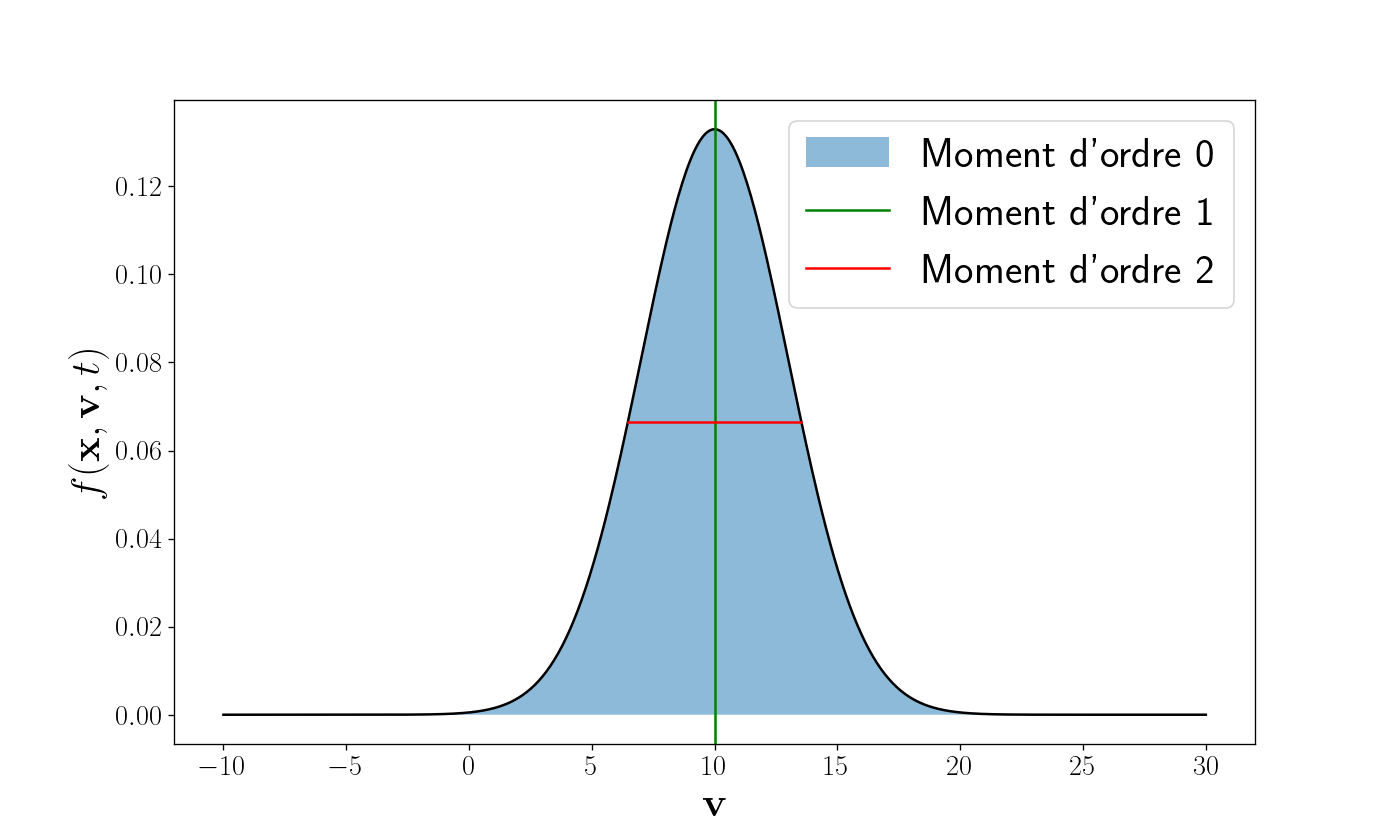
\includegraphics[width=\linewidth,trim=2cm 0cm 3cm 1cm, clip=true]{./Part_0/images/distrib}
\cprotect\caption{Représentation graphique des moments d'ordre 0 (aire sous la courbe colorée en bleu), 1 (valeur moyenne de $\mathbf{v}$ indiquée par la verticale verte) et 2 (largeur indiquée par l'horizontale rouge) de la fonction de distribution en vitesse $f\left(\mathbf{x},\mathbf{v},t\right)$ ici gaussienne.}
\label{fig:distrib}
\end{figure}
 

Suivant la fonction $g$, on peut obtenir pour chaque espèce, les quantités macroscopiques suivantes, aussi appelées <<moments>>,  : 
\begin{table}[!ht]
\begin{center}
\begin{tabular}{ c|c|c|c } 
Quantité & $\left<G\left(\mathbf{x},t\right)\right>_{\alpha}$ & $g\left(\mathbf{x},\mathbf{v},t\right)$  & ordre\\
\hline
Densité de particules & $n_{\alpha}\left(\mathbf{x},t\right)$ & $1$  & 0 \\
Densité de masse & $\rho_{\alpha}\left(\mathbf{x},t\right)$ & $m_{\alpha}\left(\mathbf{x},t\right)$ & 0 \\
Densité de charge & $Q_{\alpha}\left(\mathbf{x},t\right)$ & $q_{\alpha}\left(\mathbf{x},t\right)$ & 0\\
Densité de vitesse du fluide & $n_{\alpha} \boldsymbol{v_{\alpha}}\left(\mathbf{x},t\right)$ & $\mathbf{v}$ & 1\\
Densité de courant & $\boldsymbol{j_{\alpha}}\left(\mathbf{x},t\right)$ & $q_{\alpha} \boldsymbol{v_{\alpha}}$ & 1\\
Pression & $\overline{\boldsymbol{P_{\alpha}}} \left(\mathbf{x},t\right)$ & $m_{\alpha}\left(\mathbf{v}-\boldsymbol{v_{\alpha}}\right)\left(\mathbf{v}-\boldsymbol{v_{\alpha}}\right)$ & 2\\
Flux de chaleur& $\overline{\overline{\boldsymbol{q_{\alpha}}}}\left(\mathbf{x},t\right)$ & $m_{\alpha}\left(\mathbf{v}-\boldsymbol{v_{\alpha}}\right)\left(\mathbf{v}-\boldsymbol{v_{\alpha}}\right)\left(\mathbf{v}-\boldsymbol{v_{\alpha}}\right)$ & 3\\
\end{tabular}
\end{center}
\end{table}

À partir de l'équation de Vlasov, on obtient des équations dites <<multi-fluides>> (dépendantes de $\alpha$) décrivant l'évolution des différents moments :
\begin{itemize}
    \item L'équation de continuité pour la densité massique :
\begin{eqnarray}
  \label{eq:model_0_multi} \partial_t \rho_{\alpha} + \nabla \cdot \left(\rho_{\alpha} \boldsymbol{v_{\alpha}}\right) &=& 0.
 \end{eqnarray}
    \item L'équation sur la quantité de mouvement :
\begin{eqnarray}
  \label{eq:model_1_multi} \partial_t \left(\rho_{\alpha} \boldsymbol{v_{\alpha}}\right) + \nabla \cdot \left(\rho_{\alpha} \boldsymbol{v_{\alpha}}\boldsymbol{v_{\alpha}} + \overline{\boldsymbol{P_{\alpha}}}\right) - Q_{\alpha} \boldsymbol{E} - \boldsymbol{j_{\alpha}} \times \boldsymbol{B} &=& 0.
 \end{eqnarray}
 \item L'équation d'évolution du tenseur de pression :
\begin{eqnarray}
  \label{eq:model_2_multi} \partial_t \overline{\boldsymbol{P_{\alpha}}} + \nabla \cdot \left(\boldsymbol{v_{\alpha}}\overline{\boldsymbol{P_{\alpha}}} + \overline{\overline{\boldsymbol{q_{\alpha}}}}\right) + \left(\overline{\boldsymbol{P_{\alpha}}} \cdot \nabla \boldsymbol{v_{\alpha}}\right)^S +  \frac{Q_{\alpha}}{\rho_{\alpha}} \left(\boldsymbol{B}\times \overline{\boldsymbol{P_{\alpha}}}\right)^S  &=& 0 ,
\end{eqnarray}
\end{itemize}
avec $\left( \right)^S = \left( \right) + \left( \right)^T$ avec $\left( \right)^T$ la transposée de $\left( \right)$. Ces équations sont associées respectivement aux moments d'ordre 0, 1 et 2. On remarque que l'équation du moment d'ordre $n$ dépend d'un moment d'ordre $n+1$. Afin de fermer le système d'équations, des équations dites <<de fermeture>>, devront être introduites. 

Dans les plasmas que l'on considère, on a deux populations ($\alpha = i,e$): les ions/protons ($m_i$, $e$) et les électrons ($m_e$, $-e$) avec les masses $m_i \gg m_e$ et $e$ la charge élémentaire. Le système d'équation multi-fluide sera donc appelé <<bi-fluide>>. On l'abordera dans le Chapitre \ref{ch-23}. 

Les quantités totales (notées sans indices : $n$, $\rho$, $\boldsymbol{v}$, $\boldsymbol{j}$, etc.) sont ensuite obtenues en sommant sur toutes les espèces, $n_{\alpha}$, $\rho_{\alpha}$, $Q_{\alpha}$, $\rho_{\alpha} \boldsymbol{v_{\alpha}}$, $\boldsymbol{j_{\alpha}}$, $\overline{\boldsymbol{P_{\alpha}}} +  \rho_{\alpha} \boldsymbol{v_{\alpha}}\boldsymbol{v_{\alpha}}$ et $\rho_{\alpha} u_{\alpha} + \frac{1}{2} \rho_{\alpha} |\boldsymbol{v_{\alpha}}|^2$.  En appliquant ces sommations aux équations \eqref{eq:model_0_multi}, \eqref{eq:model_1_multi} et \eqref{eq:model_2_multi} et en considérant l'hypothèse de quasi-neutralité ($Q \simeq 0$), on obtient les équations mono-fluides quasi-neutres suivantes :
\begin{itemize}
    \item L'équation de continuité pour la densité massique :
\begin{eqnarray}
  \label{eq:model_0_mono} \Rightarrow \partial_t \rho + \nabla \cdot \left(\rho \boldsymbol{v}\right) &=& 0 .
 \end{eqnarray}
    \item L'équation sur la quantité de mouvement :
\begin{eqnarray}
\label{eq:model_1_mono} \Rightarrow \partial_t \left(\rho \boldsymbol{v}\right) + \nabla \cdot \left(\rho \boldsymbol{v}\boldsymbol{v} + \overline{\boldsymbol{P}}\right) - \boldsymbol{j} \times \boldsymbol{B} &=& 0 .
 \end{eqnarray}
 \item L'équation d'évolution du tenseur de pression, avec $\overline{\boldsymbol{P_E}} = \sum_{\alpha} \frac{Q_{\alpha}}{\rho_{\alpha}} \overline{\boldsymbol{P_{\alpha}}}$ :
\begin{eqnarray}
 \label{eq:model_2_mono} \Rightarrow \partial_t \overline{\boldsymbol{P}} + \nabla \cdot \left(\boldsymbol{v}\overline{\boldsymbol{P}} + \overline{\overline{\boldsymbol{q}}}\right) + \left(\overline{\boldsymbol{P}} \cdot \nabla \boldsymbol{v}\right)^S +  \frac{Q}{\rho} \left(\boldsymbol{B}\times \overline{\boldsymbol{P_E}}\right)^S  &=& 0 .
\end{eqnarray}
\end{itemize}
L'hypothèse non-relativiste et la quasi-neutralité permettent d'y remplacer $\boldsymbol{j}$ par $\nabla \times \boldsymbol{B}$ (Equation de Maxwell \eqref{eq:M4}).

On peut construire, à partir de l'équation \eqref{eq:model_1_multi}, l'équation d'évolution de la densité de courant totale $\boldsymbol{j} = e n_i \boldsymbol{v_i} - e n_e \boldsymbol{v_e}$. Sachant que $m_i \gg m_e$, cette équation peut s'écrire sous la forme de la loi d'Ohm généralisée : \begin{equation} 
\boldsymbol{E} =  \boldsymbol{E_{ind}} +  \boldsymbol{E_{hall}} +  \boldsymbol{E_{therm}} \label{eq:ohm} 
\end{equation}
avec :
\begin{itemize}
 \item $\boldsymbol{E_{MHD}} =  - \boldsymbol{v} \times \boldsymbol{B}$, le terme d'induction,
 \item $\boldsymbol{E_{hall}} = \lambda_i \frac{\boldsymbol{j}}{\rho} \times \boldsymbol{B}$, le terme de \acl{Hall},
 \item $\boldsymbol{E_{\nabla P_e}} = - \frac{\lambda_i}{\rho} \nabla \cdot \overline{\boldsymbol{P_{e}}}$,  \acl{Pe},
\end{itemize}
avec $\lambda_i = \frac{m_i}{e}$. La loi d'Ohm permet d'expliciter $\boldsymbol{E}$ dans l'équation \eqref{eq:M3}. En ne prenant en compte que le terme d'induction dans la loi d'Ohm, on obtient l'équation : 
\begin{equation}
    \label{eq:model_M3_ideal} \partial_t \boldsymbol{B} = \nabla \times \left(\boldsymbol{v} \times \boldsymbol{B} \right)
\end{equation}
qui s'écrit en fonction de la vitesse d'Alfvén $\boldsymbol{v_A} = \frac{\boldsymbol{B}}{\sqrt{\mu_0 \rho}}$ avec $\mu_0$, la perméabilité du vide, : 
\begin{equation}
\label{eq:model_M3_idealvA} \partial_t \boldsymbol{v_A}  =   \nabla \cdot \left(\boldsymbol{v_A}\boldsymbol{v} - \boldsymbol{v}\boldsymbol{v_A}\right) -  \boldsymbol{v}  \nabla \cdot \boldsymbol{v_A} +  \frac{\boldsymbol{v_A}}{2}  \nabla \cdot \boldsymbol{v}. \end{equation}

Les équations \eqref{eq:model_0_mono}, \eqref{eq:model_1_mono} avec l'hypothèse non-relativiste, \eqref{eq:model_2_mono} et  \eqref{eq:model_M3_ideal} forment le modèle \ac{MHD} non fermé, valable pour des échelles temporelles associées à des fréquences plus petites que la fréquence cyclotron ionique $\omega_{ci} = B_0/\lambda_i$ avec $B_0 = \left<|\boldsymbol{B}|\right>$ et des échelles spatiales, dites \ac{MHD}, plus grandes que $d_i$ et $\rho_{Li}$. En fonction de l'équation de fermeture choisie, l'équation \eqref{eq:model_2_mono} peut être omise, par exemple dans le cas d'une fermeture isotherme où $\overline{\boldsymbol{P}} \propto \rho$.
Usuellement, la pression est supposée isotrope dans le modèle \acs{MHD} mais dans ce mémoire, on ne fera cette hypothèse que dans la Partie \ref{part_1}. Dans la Partie \ref{part_2}, on abordera l'extension de la théorie des lois exactes au modèle \acs{MHDH} pour laquelle l'équation d'induction peut s'écrire : 
\begin{equation}
\partial_t \boldsymbol{v_A}  =   \nabla \cdot \left(\boldsymbol{v_A}\boldsymbol{v} - \boldsymbol{v}\boldsymbol{v_A}\right) -  \boldsymbol{v}  \nabla \cdot \boldsymbol{v_A} +  \frac{\boldsymbol{v_A}}{2}  \nabla \cdot \boldsymbol{v} - \frac{\lambda}{ \sqrt{\rho} } \nabla \times\left(\frac{1}{\sqrt{\rho}} \boldsymbol{j}\times \boldsymbol{v_A}\right)  .\label{eq:model_M3_hall}
\end{equation}
Ce modèle est souvent normalisé par la vitesse d'Alfvén moyenne $v_{A0}$. Dans l'équation \eqref{eq:model_M3_hall}, $\lambda_i$ est alors remplacée par la longueur inertielle des ions $d_i = v_{A0}\omega_{ci}$. Ce modèle sera donc valable aux échelles MHD et aux échelles dites Hall, proches de $d_i$. Certaines simulations que l'on analysera dans la Partie \ref{part_3} prennent aussi en compte le \acl{Pe}. Nous proposerons donc une extension au modèle \acs{MHDHPe}. Ce terme permet de prendre en compte la contribution thermique des électrons au champ électrique. 
%Le terme inertiel électronique, dépendant de $\lambda_e$, permet quant à lui d'accéder aux échelles électroniques proches de $d_e$ ou $\rho_{Le}$.

\section{Synthèse : problématique et modèles utilisés}
\label{synt-02}
\fcolorbox{red}{white}{\begin{minipage}[c]{\linewidth}
\paragraph{Problématique générale : } Quel est l'impact des fermetures dépendant de la pression sur la cascade turbulente ? \\

\paragraph{Plan : }
\begin{itemize}
    \item Partie \ref{part_1} : Impact d'une pression isotrope sur la cascade turbulente compressible,
    \item Partie \ref{part_2} : Description d'un écoulement turbulent dépendant d'une pression anisotrope,
    \item Partie \ref{part_3} : Effet de l'anisotropie de pression sur la cascade turbulente. \\
\end{itemize}
\end{minipage}}

\fcolorbox{blue}{white}{\begin{minipage}[c]{\linewidth}

\paragraph{Modèles utilisés}
\begin{eqnarray}
  \label{eq:synth_model_0_mono} \Rightarrow \partial_t \rho + \nabla \cdot \left(\rho \boldsymbol{v}\right) &=& 0 \\
\label{eq:synth_model_1_mono} \Rightarrow \partial_t \left(\rho \boldsymbol{v}\right) + \nabla \cdot \left(\rho \boldsymbol{v}\boldsymbol{v} + \overline{\boldsymbol{P}}\right) - \boldsymbol{j} \times \boldsymbol{B} &=& 0 \\
 \label{eq:synth_model_2_mono} \Rightarrow \partial_t \overline{\boldsymbol{P}} + \nabla \cdot \left(\boldsymbol{v}\overline{\boldsymbol{P}} + \overline{\overline{\boldsymbol{q}}}\right) + \left(\overline{\boldsymbol{P}} \cdot \nabla \boldsymbol{v}\right)^S +  \left(\boldsymbol{B}\times \overline{\boldsymbol{P_E}}\right)^S  &=& 0 
\end{eqnarray}
\begin{itemize}
\item \ac{MHD} (Parties \ref{part_1} et \ref{part_2}) : 
\begin{equation}
    \label{eq:synth_M3_ideal} \partial_t \boldsymbol{B} = \nabla \times \left(\boldsymbol{v} \times \boldsymbol{B} \right)
\end{equation}
\item \acs{MHDH} (Parties \ref{part_2} et \ref{part_3}) : 
\begin{equation}
    \label{eq:synth_M3_hall} \partial_t \boldsymbol{B} = \nabla \times \left(\boldsymbol{v} \times \boldsymbol{B} \right) - \lambda \nabla \times \left( \frac{\boldsymbol{j}}{\rho} \times \boldsymbol{B} \right)
\end{equation}
\item \acs{MHDHPe} (Parties \ref{part_2} et \ref{part_3}) : 
\begin{equation}
    \label{eq:synth_M3_gpe} \partial_t \boldsymbol{B} = \nabla \times \left(\boldsymbol{v} \times \boldsymbol{B} \right) - \lambda \nabla \times \left( \frac{\boldsymbol{j}}{\rho} \times \boldsymbol{B} \right) + \lambda \nabla \times \left( \frac{1}{\rho} \nabla \cdot \overline{\boldsymbol{P_{e}}}\right)
\end{equation}
\item Autre : Bi-fluide (Parties \ref{part_2})\\
\end{itemize}

\end{minipage}}

\chapter{Etude de la cascade turbulente dans un plasma incompressible}
\renewcommand\partie{\Partie\ Chapitre \thechapter}
\label{ch-11}

%\medskip
\minitoc  

\bigskip

Ce n'est que 57 ans après l'apport de Kolmogorov à la compréhension de la turbulence que l'idée de chercher des lois exactes dans un fluide magnétisé, ou plasma, a émergé. Ainsi, \cite{politano_von_1998} et \cite{politano_dynamical_1998} ont étendu la théorie hydrodynamique à la \ac{MHD} en restant dans le cadre incompressible. Cette avancée historique a apporté un cadre à l'étude de la turbulence dans les plasmas spatiaux. Dans le laboratoire qu'est le vent solaire, elle a permis de trouver des éléments de réponse à des problèmes tels que ceux du chauffage ou de l'accélération du vent [\cite{smith_dependence_2006,sorriso-valvo_observation_2007,stawarz_turbulent_2009,osman_proton_2013,bruno_solar_2013,alexandrova_solar_2013,sahraoui_magnetohydrodynamic_2020,marino_scaling_2023}]. 

Le modèle incompressible magnétohydrodynamique idéal avec pression isotrope (\acs{IMHD}) est la description fluide d'un plasma la plus simple abordée dans ce mémoire. Dans ce chapitre, nous reprendrons les résultats analytiques incompressibles principaux afin d'introduire les outils fondamentaux de l'étude de la turbulence dans un plasma.

\section{Le modèle et l'énergie totale}
\label{sec-111}
Contrairement au modèle hydrodynamique incompressible abordé dans le Chapitre \ref{ch-01}, dans le cas d'un plasma, il est nécessaire de prendre en compte le couplage entre le fluide et le champ magnétique et d'ajouter l'équation d'induction \eqref{eq:synth_M3_ideal} comme on a pu le mettre en pratique dans le Chapitre \ref{ch-02}. L'incompressibilité s'exprime quant à elle à travers la contrainte $\nabla \cdot \boldsymbol{v} = 0$. Le modèle magnétohydrodynamique incompressible (\acs{IMHD}) est alors :
\begin{eqnarray}
\label{eq:model_inc_v} \partial_t \boldsymbol{v} + \boldsymbol{v} \cdot \nabla \boldsymbol{v} -  \boldsymbol{v_A} \cdot \nabla \boldsymbol{v_A} + \frac{1}{\rho_0} \nabla p_* &=& 0, \\
\label{eq:model_inc_b} \partial_t \boldsymbol{v_A} + \boldsymbol{v} \cdot \nabla \boldsymbol{v_A} -  \boldsymbol{v_A} \cdot \nabla \boldsymbol{v}&=& 0, \\
\label{eq:model_inc_r} \nabla \cdot \boldsymbol{v} &=& 0.
\end{eqnarray}
Le champ magnétique apparaît dans ces équations à travers la vitesse d'Alfvén $\boldsymbol{v_A} = \boldsymbol{B}/\sqrt{\mu_0 \rho_0}$ et la pression magnétique $p_m = \rho_0 \boldsymbol{v_A}^2 /2$ contenue dans la pression totale $p_* = p + p_m$. On remarque qu'il y a 3 équations (7 en termes de composantes) et 3 inconnues (2 vectorielles, $\boldsymbol{v}$ et $\boldsymbol{v_A}$ et une scalaire, $p$). Le système se retrouve donc fermé grâce à la contrainte incompressible en équation \eqref{eq:model_inc_r}. On peut rappeler aussi que le champ magnétique est aussi contraint tel que $\nabla \cdot \boldsymbol{B} = 0$, ce qui implique dans le cas incompressible : $\nabla \cdot \boldsymbol{v_A} = 0$ (contrainte implicitement prise en compte dans l'équation d'induction \eqref{eq:model_inc_b}). En appliquant la divergence sur l'équation \eqref{eq:model_inc_v}, on obtient l'équilibre de pression, $- \frac{1}{\rho_0}\nabla^2 p_* = \nabla \boldsymbol{v} : \nabla \boldsymbol{v} -  \nabla \boldsymbol{v_A} : \nabla \boldsymbol{v_A} $, qui indique que la pression totale est directement reliée aux non-linéarités du système.\footnote{Ce système peut aussi être symétrisé grâce aux variables d'Elsässer, $\boldsymbol{z^{\pm}} = \boldsymbol{v} \pm \boldsymbol{v_A}$: 
\begin{eqnarray}
\partial_t \boldsymbol{z^{\pm}} + \boldsymbol{z^{\mp}} \cdot \nabla \boldsymbol{z^{\pm}} = - \frac{1}{\rho_0} \nabla p_* , &\qquad& \nabla \cdot \boldsymbol{z^{\pm}} = 0 .
\end{eqnarray}
Leur somme $\frac{1}{4}\rho_0 (\boldsymbol{z^{+}}{}^2 + \boldsymbol{z^{-}}{}^2)$ donne l'énergie totale $E_{tot}$ et leur différence, l'hélicité croisée  $H_c$. La dynamique non-linéaire est alors contenue dans le terme $\boldsymbol{z^{\mp}} \cdot \nabla \boldsymbol{z^{\pm}}$. De telles variables sont adaptées à l'étude de ce système incompressible et sont largement utilisées pour simplifier les calculs. Il est nécessaire de garder en tête qu'en termes de mathématique fondamentale, elles ne peuvent exister, car elles sont la somme d'un champ vectoriel (vitesse) et d'un champ pseudo-vectoriel (champ magnétique). Dans un effort de cohérence avec le cadre compressible dans lequel elles sont mal définies [\cite{magyar_nature_2019}], elles ne seront pas utilisées ici.}

Dans ce système apparaissent deux canaux énergétiques : cinétique de densité $E_c = \frac{1}{2} \rho_0 \boldsymbol{v}^2$, et magnétique, $E_m = \frac{1}{2} \rho_0 \boldsymbol{v_A}^2$. On définit aussi la densité d'hélicité croisée couplant les deux champs : $H_c = \rho_0 \boldsymbol{v_A} \cdot \boldsymbol{v}$. Les équations de densité d'énergie cinétique et magnétique, obtenue respectivement à partir de \eqref{eq:model_inc_v} et  \eqref{eq:model_inc_b}, et celle de densité d'énergie totale $E_{tot} = E_c + E_m$ sont alors : 
\begin{eqnarray}
 \label{eq:model_inc_k} \partial_t E_c +   \nabla  \cdot (E_c \boldsymbol{v}+ H_c \boldsymbol{v_A} + p_* \boldsymbol{v}  )  &=& - \rho_0  \boldsymbol{v_A} \boldsymbol{v_A} : \nabla \boldsymbol{v}, \\
 \label{eq:model_inc_m} \partial_t E_m +   \nabla  \cdot (E_m \boldsymbol{v}) &=& \rho_0   \boldsymbol{v_A} \boldsymbol{v_A} : \nabla \boldsymbol{v} ,\\
\label{eq:model_inc_e} \partial_t E_{tot} +   \nabla  \cdot (E_{tot} \boldsymbol{v} + H_c \boldsymbol{v_A} + p_* \boldsymbol{v} )  &=&  0.
\end{eqnarray}
L'équation \eqref{eq:model_inc_e} indique que la densité d'énergie totale moyenne $\left<E_{tot}\right>$ est conservée puisque pour toute quantité $\boldsymbol{X}$, la moyenne, ici spatiale, $\left<\right>$, implique\footnote{En supposant la périodicité de $\boldsymbol{X}$ ou son annulation à l'infinie.} $\left<\nabla \cdot \boldsymbol{X}\right> = 0$. Les équations \eqref{eq:model_inc_k} et \eqref{eq:model_inc_m} nous indiquent un échange entre les canaux énergétiques se faisant à travers le terme de droite. 

\section{Le cas linéaire et les ondes d'Alfvén}
La théorie linéaire est la principale voie nous donnant des informations ondulatoires sur un modèle. Ainsi, dans le modèle \acs{IMHD}, elle vient révéler l'existence des ondes dites d'Alfvén. 

Pour cela, on doit linéariser le système, c'est-à-dire négliger tout terme non-linéaire (d'ordre supérieur à 1). 
Les moyennes des quantités impliquées seront indiquée par un 0 (ordre 0) et les fluctuations d'ordre 1 seront indiquées par un 1. Ainsi, par exemple, $\boldsymbol{v} \simeq \boldsymbol{v_{0}} + \boldsymbol{v_{1}}$. On considèrera aussi que $\boldsymbol{v_{0}} = 0$ et on notera la direction du champ magnétique moyen $\boldsymbol{b_0}$. 

\label{sec-112}
\begin{wrapfigure}{r}{0.5\textwidth}
 \centering
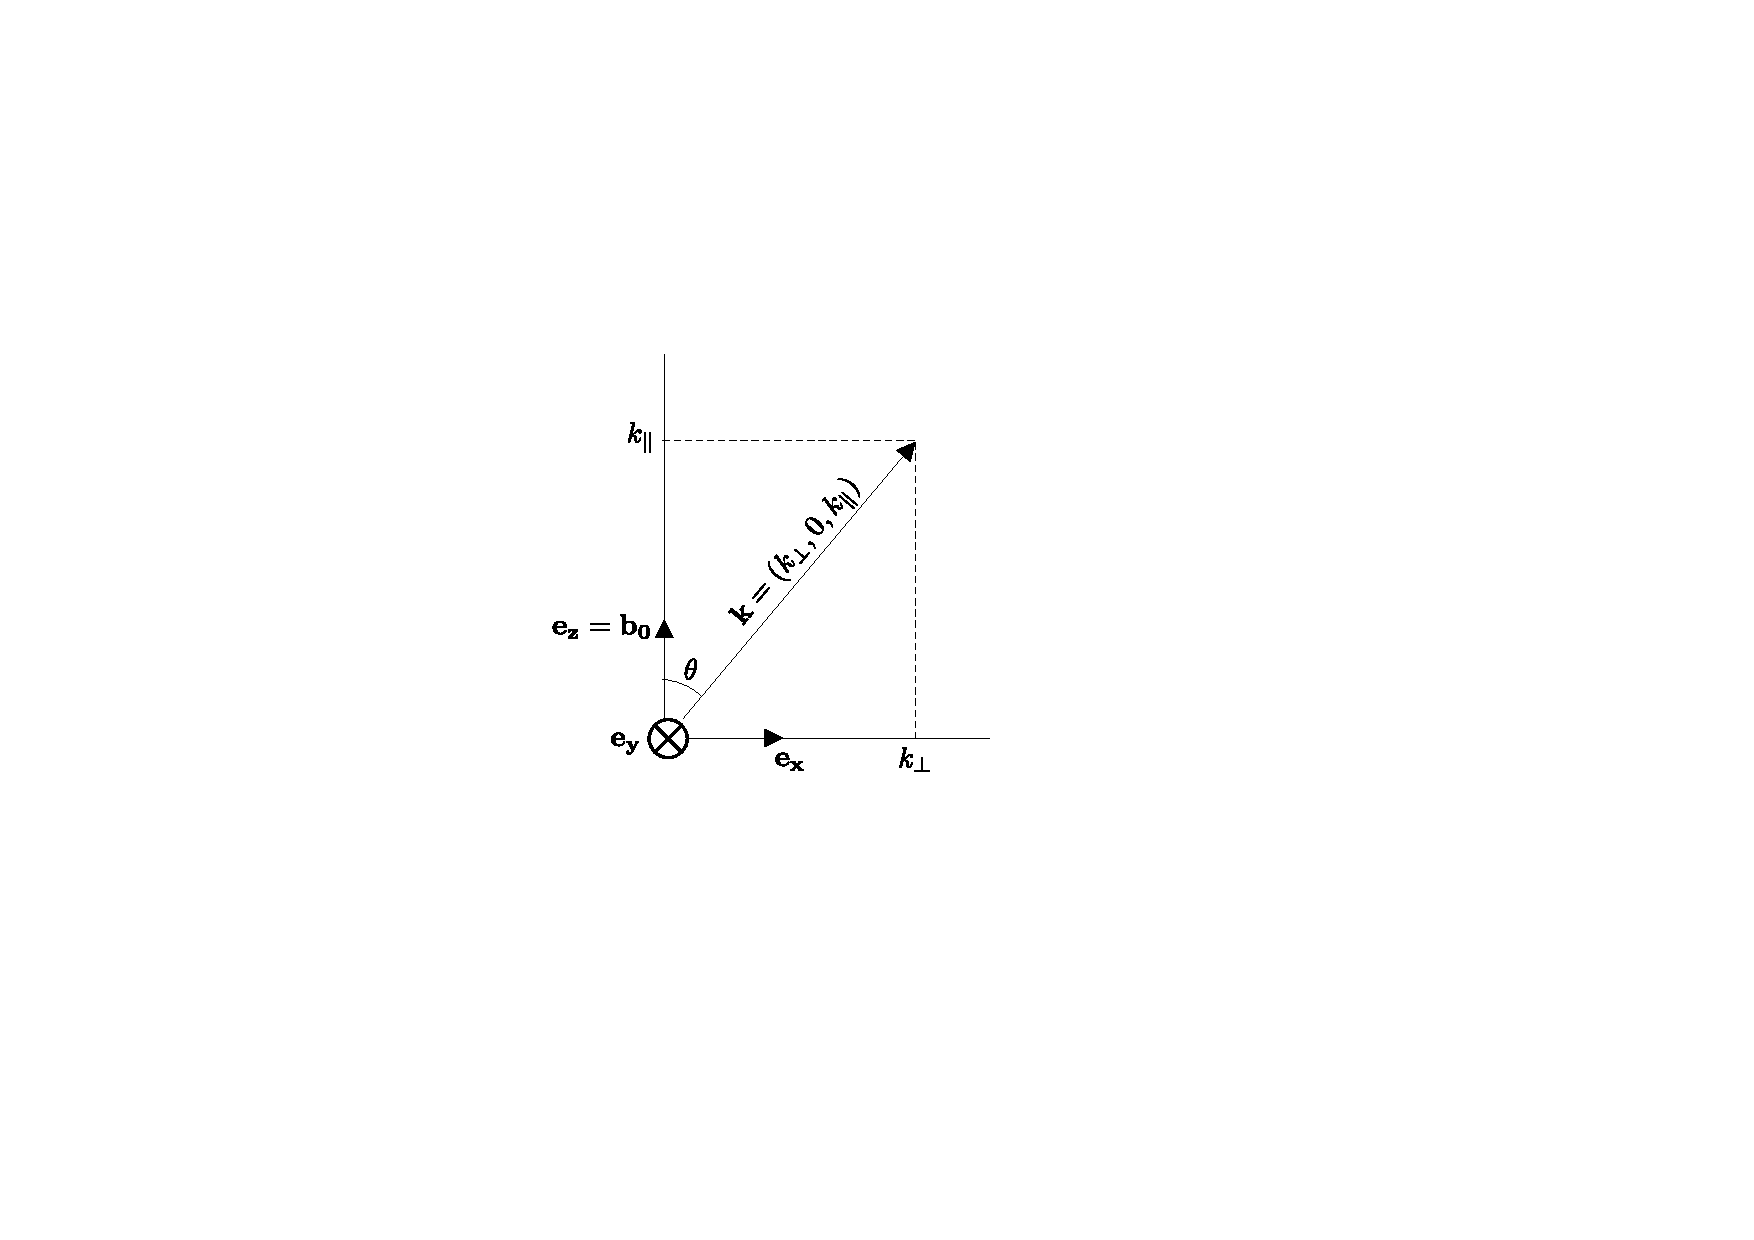
\includegraphics[width=0.6\linewidth,trim=9.3cm 7.8cm 13cm 7cm, clip=true]{./Part_1/images/schema_kplan.pdf}
\caption{Système de coordonnées et vecteur d'onde dans le cadre linéaire.}
\label{fig:schema_kplan}
\end{wrapfigure}

La deuxième étape consiste à passer dans l'espace de Fourier, c'est-à-dire remplacer $\partial_t$ par la pulsation $-i\omega$ et $\nabla$ par le vecteur d'onde $i\boldsymbol{k}$. On supposera sans perte de généralité, le système de coordonnées cartésiennes orienté tel que $\boldsymbol{e_z} = \boldsymbol{b_0}$ et la composante suivant $\boldsymbol{e_y}$ du vecteur d'onde, $k_y = 0$. On notera $k$ la norme du vecteur d'onde, $k_{\parallel}$ sa composante le long de $\boldsymbol{e_z}$, parallèle au champ magnétique moyen, $k_{\perp}$ sa composante le long de $\boldsymbol{e_x}$ et $\theta$ l'angle formé avec $\boldsymbol{e_z}$ (voir \figref{fig:schema_kplan}).
Le système \acs{IMHD} devient alors : 
\begin{eqnarray}
 \label{eq:lin_inc_v} \omega \boldsymbol{v_{1}}  + v_{A0} k_{\parallel} \boldsymbol{v_{A1}} - \frac{1}{\rho_0}  p_{*1} \boldsymbol{k}&=& 0 ,\\
 \label{eq:lin_inc_b} \omega \boldsymbol{v_{A1}}  +  v_{A0} k_{\parallel}  \boldsymbol{v_{1}}&=& 0 ,\\
 \label{eq:lin_inc_r} \boldsymbol{k} \cdot \boldsymbol{v_{1}} = 0 \qquad \boldsymbol{k} \cdot \boldsymbol{v_{A1}}  &=& 0 .
\end{eqnarray}

Ensuite, on injecte les équations \eqref{eq:lin_inc_b} et \eqref{eq:lin_inc_r} dans l'équation \eqref{eq:lin_inc_v} : 
\begin{itemize}
    \item $\boldsymbol{k} \cdot \eqref{eq:lin_inc_v} \Rightarrow  p_{*1} =0$, en excluant le cas trivial où $\boldsymbol{k}=0$. La pression totale n'est donc bien reliée qu'aux non-linéarités du système.
    \item $\omega \cdot \eqref{eq:lin_inc_v} \Rightarrow (\omega^2   - (\boldsymbol{k} \cdot \boldsymbol{v_{A0}})^2 ) \boldsymbol{v_{1}} = 0$ (dite équation de dispersion), d'où la relation de dispersion :  
    \begin{equation}
        \label{eq:lin_inc_disp} \omega = \pm \boldsymbol{k} \cdot \boldsymbol{v_{A0}} = \pm v_{A0} k_{\parallel} =  \pm v_{A0} k \cos \theta .
    \end{equation}
    \item \eqref{eq:lin_inc_b} et \eqref{eq:lin_inc_disp} $ \Rightarrow \boldsymbol{v_{1}} = \pm \boldsymbol{v_{A1}}$.
    \item $ p_{*1} =0 \Rightarrow p_{1} = - v_{A0} v_{A1z}$ .
\end{itemize}
La relation de dispersion \eqref{eq:lin_inc_disp} nous indique qu'il peut y avoir dans le système \acs{IMHD}, des ondes dites d'Alfvén, couplant champ magnétique et champ de vitesse. 
Généralement, pour obtenir la polarisation d'une onde, on injecte sa relation de dispersion dans le système. Dans le cas du système \acs{IMHD}, le système s'annule alors complètement. La polarisation de l'onde d'Alfvén dans le cas \acs{IMHD}, est définie par $\boldsymbol{k} \cdot \boldsymbol{v_{A1}}  = 0 $ qui indique que $\boldsymbol{v_{A1}} $ doit être perpendiculaire à $\boldsymbol{k}$. Or $\boldsymbol{k}$ est dans le plan $\boldsymbol{e_x}-\boldsymbol{e_z}$. Donc $\boldsymbol{v_{A1}} $ est polarisé suivant une combinaison linéaire des vecteurs $\boldsymbol{e_y}$ et $(-\cos \theta, 0, \sin \theta)$. Le mode d'Alfvén est donc dégénéré, il est formé d'un mode dit incompressible, polarisé suivant $\boldsymbol{e_y}$, et d'un mode dit pseudo-alfvénique, polarisé suivant $(-\cos \theta, 0, \sin \theta)$.

L'onde d'Alfvén est très importante en physique des plasmas, elle est, en effet, solution exacte du système \acs{IMHD} linéaire et non linéaire. En turbulence, elle peut donc alimenter la cascade. Lorsque la cascade est développée par des ondes, on parlera de turbulence d'onde. De plus, deux régimes existent :  la turbulence faible où la cascade d'énergie est supposément développée par des interactions faiblement non-linéaires entre paquets d'ondes et, la turbulence forte où ondes et structures cohérentes (de type vortex par exemple) coexistent et entretiennent la cascade. 

\section{Décrire la cascade turbulente incompressible avec une loi exacte}
\label{sec-113}
La théorie des lois exactes, nommée ainsi car aucune hypothèse de linéarisation ou perturbative n'est supposée pour les obtenir, s'appuie sur les hypothèses de Kolmogorov exposées et illustrées dans le Chapitre \ref{ch-01} (voir synthèse \ref{synt-01}) et rappelées ci-après. On se réfèrera au chapitre \ref{ch-01} à propos des notations. Historiquement, de multiples versions de la loi exacte décrivant la cascade \acs{IMHD} et de la méthode pour l'obtenir existent [\cite{politano_von_1998,galtier_origin_2018,macbride_turbulent_2008}]. On la nommera dans la suite \acs{PP98} du nom des deux chercheuses ayant dérivé la première version en 1998.

D'après les hypothèses de Kolmogorov, la zone inertielle est définie comme l'ensemble des échelles où le tranfert s'effectue conservativement. L'énergie totale (cinétique + magnétique) étant un invariant du système \acs{IMHD}, elle peut a priori cascader de manière conservative. 
Une cascade d'énergie implique une source d'injection et un canal de dissipation, respectivement aux grandes et petites échelles. Le canal de dissipation transfert l'énergie des champs électromagnétiques vers les particules du plasma. Cette énergie sera visible dans la fonction de distribution des particules à travers une augmentation de sa largeur (chauffage) ou un décalage de la moyenne (accélération). Dans le cadre \acs{IMHD}, les dissipations généralement admises sont des dissipations visqueuses ou résistives qui s'accompagnent d'une variation d'entropie. 
Le canal d'injection est nécessaire pour entretenir la cascade et compenser la dissipation dans le bilan énergétique (dans le cas incompressible) [\cite{galtier_physique_2021}]. Pour refléter cela dans les équations, on va ajouter une force $\boldsymbol{f_c}$ d'injection agissant à grande échelle et un terme dissipatif (visqueux), $\boldsymbol{d_c}$, agissant à petite échelle, dans l'équation \eqref{eq:model_inc_v} et, pour permettre la visualisation de ce que deviennent ces sources si elles sont définies magnétiquement, on va ajouter $\boldsymbol{f_m}$ et $\boldsymbol{d_m}$ (résistif) dans l'équation d'induction \eqref{eq:model_inc_b}. On restera dans un cadre général en ne détaillant pas leur contenu. Ainsi :
\begin{eqnarray}
\label{eq:turb_inc_v} \partial_t \boldsymbol{v} + \boldsymbol{v} \cdot \nabla \boldsymbol{v} -  \boldsymbol{v_A} \cdot \nabla \boldsymbol{v_A} + \frac{1}{\rho_0} \nabla p_* &=&  \boldsymbol{f_c} + \boldsymbol{d_c} , \\
\label{eq:turb_inc_b}  \partial_t \boldsymbol{v_A} + \boldsymbol{v} \cdot \nabla \boldsymbol{v_A} -  \boldsymbol{v_A} \cdot \nabla \boldsymbol{v}&=& \boldsymbol{f_m} + \boldsymbol{d_m} ,\\
\label{eq:turb_inc_r}  \nabla \cdot \boldsymbol{v} = 0, && \nabla \cdot \boldsymbol{v_A} = 0.
\end{eqnarray}

Maintenant, si l'on veut une loi exacte sur l'énergie totale, on doit choisir une fonction de corrélation qui, lorsque $\boldsymbol{x'}= \boldsymbol{x}$, est égale à l'énergie totale moyenne, ici $\left<E_{tot}\right> = \left<E_c + E_m\right> = \left<\frac{1}{2} \rho_0 \boldsymbol{v}^2 + \frac{1}{2} \rho_0 \boldsymbol{v_A}^2\right>$. Cela nous donne bien des choix de formulation : 
\[\left<\sqrt{E_{tot}} \cdot \sqrt{E'_{tot}}\right>, \qquad \left<\sqrt{E_c} \cdot \sqrt{E'_c} + \sqrt{E_m} \cdot \sqrt{E'_m} \right>,\] et pourquoi pas d'autres puissances ? Ici, c'est la même quantité à une constante près, mais on pourrait avoir à choisir en $\boldsymbol{B}$ ou $\boldsymbol{v_A}$, ou encore utiliser les variables d'Elsässer. Une autre possibilité est de définir cette fonction à l'aide des incréments de quantités (voir par exemple \cite{antonia_analogy_1997}). Avec une telle fonction, on obtient naturellement son annulation lorsque $\boldsymbol{x'}= \boldsymbol{x}$. Du choix de la fonction de corrélation va dépendre la difficulté du calcul, la sauvegarde du sens physique (que voudrait dire $\boldsymbol{v}^{1/5}$ ?) et potentiellement l'élégance et la compacité du résultat. Une question fondamentale subsiste et ne sera qu'en partie traitée dans cette thèse : regarde-t-on la même chose quel que soit le choix de fonction de corrélation ?\footnote{On regardera la différence analytique entre les fonctions de type incrémentale ou non (traitée numériquement dans les cadres \ac{MHDH} incompressible et compressible par [\cite{ferrand_exact_2019,ferrand_-depth_2022}]). La question de la convergence des taux de cascade obtenus avec des lois du même type (incrémental ou non) mais différentes formulations (exemple des différentes puissances) reste un problème ouvert qui n'a, à notre connaissance, pas été traité rigoureusement.} On prendra comme exemple la fonction d'auto-corrélation pour chaque canal d'énergie : $\mathcal{R} = \frac{1}{2} \rho_0\left< \boldsymbol{v} \cdot \boldsymbol{v'} + \boldsymbol{v_A} \cdot \boldsymbol{v'_A}\right>$, $\rho_0/2$ étant une constante dans ce cadre incompressible. 

Ensuite, on doit dériver une équation pour cette fonction de corrélation, elle s'obtient en notant que $\partial_t \mathcal{R} = \frac{1}{2} \rho_0 (\left<\partial_t(\boldsymbol{v}) \cdot \boldsymbol{v'} + \boldsymbol{v} \cdot \partial_t(\boldsymbol{v'}) \right> + \left<\partial_t(\boldsymbol{v_A}) \cdot \boldsymbol{v'_A} + \boldsymbol{v_A} \cdot \partial_t(\boldsymbol{v'_A}) \right>)$ et en remplaçant les dérivées temporelles grâce aux équations \eqref{eq:turb_inc_v} et \eqref{eq:turb_inc_b}. Pour alléger la démonstration, on peut noter que $\left<\partial_t(\boldsymbol{v'}) \cdot \boldsymbol{v}\right> $ est le conjugué de $\left<\partial_t(\boldsymbol{v}) \cdot \boldsymbol{v'}\right> $, c'est-à-dire en échangeant les rôles (prime ou pas) de chacun des points. Ainsi, on obtient en jouant un peu avec l'hypothèse d'homogénéité statistique et les contraintes \eqref{eq:turb_inc_r} : 
\begin{eqnarray}
\label{eq:turb_inc_v1} \left<\boldsymbol{v'} \cdot \partial_t \boldsymbol{v}\right> &=&  \nabla_{\boldsymbol{\ell}} \cdot \left< \boldsymbol{v'} \cdot \boldsymbol{v}\boldsymbol{v}-\boldsymbol{v'} \cdot \boldsymbol{v_A}   \boldsymbol{v_A}\right> +  \left<\boldsymbol{v'} \cdot \boldsymbol{f_c}+\boldsymbol{v'} \cdot \boldsymbol{d_c}\right> ,\\
\label{eq:turb_inc_b1}\left<\boldsymbol{v'_A} \cdot \partial_t \boldsymbol{v_A}\right> &=& \nabla_{\boldsymbol{\ell}} \cdot \left< \boldsymbol{v'_A} \cdot \boldsymbol{v_A}\boldsymbol{v}-\boldsymbol{v'_A} \cdot \boldsymbol{v}\boldsymbol{v_A}\right>  +  \left<\boldsymbol{v'_A} \cdot \boldsymbol{f_m}+\boldsymbol{v'_A} \cdot \boldsymbol{d_m}\right>,
\end{eqnarray}
puisque $ - \left<\boldsymbol{v'} \cdot \nabla p_*\right> = \nabla_{\boldsymbol{\ell}} \cdot \left< p_* \boldsymbol{v'}\right> = \left<p_* \nabla' \cdot \boldsymbol{v'}\right> = 0$. 

On peut  chercher à faire apparaître par factorisation dans les termes dit <<de flux>> (sous l'opérateur $\nabla_{\boldsymbol{\ell}} $) des équations \eqref{eq:turb_inc_v1} et \eqref{eq:turb_inc_b1}, des fonctions de structure, c'est-à-dire des multiplications d'incréments tel que $\left<\delta \boldsymbol{v} \cdot \delta \boldsymbol{v} \delta \boldsymbol{v} \right>$. Via les hypothèses d'homogénéité et les contraintes \eqref{eq:turb_inc_r}, on peut faire ainsi ressortir : 
\begin{eqnarray}
\label{eq:turb_inc_fs1} \nabla_{\boldsymbol{\ell}} &\cdot& \left<\delta \boldsymbol{v} \cdot \delta \boldsymbol{v} \delta \boldsymbol{v} \right> \nonumber \\
 &=&  \nabla_{\boldsymbol{\ell}} \cdot \left<  \boldsymbol{v'} \cdot \boldsymbol{v'} \boldsymbol{v'} - \boldsymbol{v} \cdot \boldsymbol{v} \boldsymbol{v} - \boldsymbol{v'} \cdot \boldsymbol{v'} \boldsymbol{v} + \boldsymbol{v} \cdot \boldsymbol{v} \boldsymbol{v'} + 2 \boldsymbol{v} \cdot \boldsymbol{v'} \boldsymbol{v} - 2 \boldsymbol{v'} \cdot \boldsymbol{v} \boldsymbol{v'}\right>  \nonumber\\
  &=& 2 \nabla_{\boldsymbol{\ell}} \cdot \left< \boldsymbol{v} \cdot \boldsymbol{v'} \boldsymbol{v} - \boldsymbol{v'} \cdot \boldsymbol{v} \boldsymbol{v'}\right>.
\end{eqnarray}
Et de même : 
\begin{eqnarray}
\label{eq:turb_inc_fs2}  \nabla_{\boldsymbol{\ell}} \cdot \left<\delta \boldsymbol{v_A} \cdot \delta \boldsymbol{v_A} \delta \boldsymbol{v} \right>  &=& 2 \nabla_{\boldsymbol{\ell}} \cdot \left< \boldsymbol{v_A} \cdot \boldsymbol{v'_A} \boldsymbol{v} - \boldsymbol{v'_A} \cdot \boldsymbol{v_A} \boldsymbol{v'}\right> ,\\
\label{eq:turb_inc_fs3}   \nabla_{\boldsymbol{\ell}} \cdot \left<\delta \boldsymbol{v} \cdot \delta \boldsymbol{v_A} \delta \boldsymbol{v_A} \right>  &=&  \nabla_{\boldsymbol{\ell}} \cdot \left< \boldsymbol{v} \cdot \boldsymbol{v'_A} \boldsymbol{v_A} - \boldsymbol{v'} \cdot \boldsymbol{v_A} \boldsymbol{v'_A} + \boldsymbol{v'} \cdot \boldsymbol{v_A} \boldsymbol{v_A} - \boldsymbol{v} \cdot \boldsymbol{v'_A} \boldsymbol{v'_A}\right> .\quad
\end{eqnarray}
Les fonctions de structure d'ordre 3, $\left<\delta \boldsymbol{v} \cdot \delta \boldsymbol{v} \delta \boldsymbol{v} \right>$ et $\left<\delta \boldsymbol{v_A} \cdot \delta \boldsymbol{v_A} \delta \boldsymbol{v} \right>$, rappellent la convection de l'énergie, respectivement cinétique et magnétique, par le champ de vitesse et présente dans l'équation d'énergie totale \eqref{eq:model_inc_e}, et $\left<\delta \boldsymbol{v} \cdot \delta \boldsymbol{v_A} \delta \boldsymbol{v_A} \right>$ rappelle la convection de l'hélicité croisée par le champ magnétique.

Ainsi, l'équation de la fonction de corrélation de l'énergie totale obtenue avec $\mathcal{R} = \left<\frac{1}{2} \rho_0 \boldsymbol{v} \cdot \boldsymbol{v'} + \frac{1}{2} \rho_0 \boldsymbol{v_A} \cdot \boldsymbol{v'_A}\right>$ peut s'écrire :
\begin{eqnarray}
\label{eq:turb_inc_KHM}    \partial_t \mathcal{R} &=& \frac{1}{4} \rho_0 \nabla_{\boldsymbol{\ell}} \cdot \left< \delta \boldsymbol{v} \cdot \delta \boldsymbol{v} \delta \boldsymbol{v} + \delta \boldsymbol{v_A} \cdot \delta \boldsymbol{v_A} \delta \boldsymbol{v} + 2 \delta \boldsymbol{v} \cdot \delta \boldsymbol{v_A} \delta \boldsymbol{v_A}\right> \\
 \label{eq:turb_inc_KHMinj}    &&+ \frac{1}{2} \rho_0  \left<\boldsymbol{v'} \cdot \boldsymbol{f_c} + \boldsymbol{v} \cdot \boldsymbol{f'_c} + \boldsymbol{v'_A} \cdot \boldsymbol{f_m} + \boldsymbol{v_A} \cdot \boldsymbol{f'_m}\right> \\
 \label{eq:turb_inc_KHMdiss}    &&+ \frac{1}{2} \rho_0 \left<\boldsymbol{v'} \cdot \boldsymbol{d_c} +\boldsymbol{v} \cdot \boldsymbol{d'_c} + \boldsymbol{v'_A} \cdot \boldsymbol{d_m} + \boldsymbol{v_A} \cdot \boldsymbol{d'_m}\right>.
\end{eqnarray}
Dans le terme de droite, la première ligne décrit la cascade non-linéaire ($\varepsilon_{NL} = $  \eqref{eq:turb_inc_KHM}), la deuxième, l'injection au taux $\varepsilon_F$ ($=$ \eqref{eq:turb_inc_KHMinj}), et la troisième, la dissipation ($\varepsilon_D =$  \eqref{eq:turb_inc_KHMdiss}). Les contributions magnétiques viennent se mêler aux contributions cinétiques présentes dans chaque taux et vues dans le cadre \ac{HD} (voir Chapitre \ref{ch-01}).  Cette équation du type \acs{KHM} est valable dans et en dehors de la zone inertielle. 

En $\boldsymbol{\ell} = 0$, on retrouve l'équation de densité d'énergie totale moyenne du système : $\partial_t \left<E_{tot}\right> = \left<E_F\right> + \left<E_D\right>$ avec $\left<E_F\right> = \rho_0 \left<\boldsymbol{v} \cdot \boldsymbol{f_c} + \boldsymbol{v_A} \cdot \boldsymbol{f_m} \right>$, la densité d'énergie moyenne injectée et $\left<E_D\right> = \rho_0 \left<\boldsymbol{v} \cdot \boldsymbol{d_c} + \boldsymbol{v_A} \cdot \boldsymbol{d_m}\right>$, la densité d'énergie moyenne dissipée. 
Si le système est conservatif, $\left<E_F\right> = -  \left<E_D\right> $. Afin que $\left<E_F\right> = -  \left<E_D\right>$ soit respecté $\varepsilon_F$ ne doit pas s'annuler aux échelles où le forçage n'a pas d'influence mais plutôt être égal à $\left<E_F\right>$. $\varepsilon_F (\ell)$ ne représente donc pas l'énergie qui est injectée à l'échelle $\ell$ mais plutôt l'énergie qui a été injectée dans la cascade aux échelles $>\ell$, où le forçage est actif.

En appliquant l'hypothèse de séparation d'échelle, on obtient la loi de type K41 donnée par $\varepsilon = - \varepsilon_{NL}$ : 
\begin{eqnarray}
\label{eq:turb_inc_ELK}     \varepsilon &=& - \frac{1}{4} \rho_0 \nabla_{\boldsymbol{\ell}} \cdot \left< \delta \boldsymbol{v} \cdot \delta \boldsymbol{v} \delta \boldsymbol{v} + \delta \boldsymbol{v_A} \cdot \delta \boldsymbol{v_A} \delta \boldsymbol{v} + 2 \delta \boldsymbol{v} \cdot \delta \boldsymbol{v_A} \delta \boldsymbol{v_A}\right> .
\end{eqnarray}
Cette équation est la loi exacte \acs{PP98} pour l'énergie totale du modèle \acs{IMHD}, obtenue à partir de la théorie de Kolmogorov. Ce lien entre le taux de cascade et l'anomalie dissipative $\varepsilon$ (voir synthèse \ref{synt-01}) nous permet, dans le vent solaire par exemple, d'estimer le taux de dissipation permise par la turbulence pour répondre par exemple au problème du chauffage (décrit dans le chapitre \ref{ch-02}, voir aussi [\cite{smith_dependence_2006,sorriso-valvo_observation_2007,stawarz_turbulent_2009,osman_proton_2013}]). 

Phénoménologiquement, $\varepsilon$ étant supposé constant et avec l'hypothèse d'isotropie, on remarque que : $(\delta \boldsymbol{v})^3 \sim (\delta \boldsymbol{v_A})^3 \sim \varepsilon \ell => (\delta \boldsymbol{v})^2 \sim (\delta \boldsymbol{v_A})^2 \sim \ell^{2/3}$, ce qui donne les spectres 1D d'énergie cinétique et magnétique en $E(k) \sim k(\delta \boldsymbol{v}(k))^2  \sim k(\delta \boldsymbol{v_A}(k))^2  \sim k^{-5/3}$. On retrouve ainsi la loi phénoménologique des spectres en $-5/3$ de Kolmogorov étendue aux fluides magnétisés.\footnote{Lorsque le champ magnétique est important, de l'anisotropie apparait dans l'espace de Fourier entre la direction parallèle au champ magnétique et le plan perpendiculaire. La description phénoménologique doit donc être modifiée, par exemple avec la condition dite de "critical balance" [\cite{goldreich_toward_1995,horbury_anisotropic_2008}].}

Pour en revenir à la différence entre les fonctions de corrélation, regardons ce qu'il se passe si l'on considère une fonction incrémentale, par exemple $\mathcal{S} =  \left<\frac{1}{2} \rho_0 \delta \boldsymbol{v}^2 + \frac{1}{2} \rho_0 \delta \boldsymbol{v_A}^2\right>$ formée de fonctions de structure d'ordre 2 qui rappelle celles d'ordre 3 impliquées dans le taux de cascade. On remarque que $\mathcal{S} = 2\left<E_{tot}\right> - 2\mathcal{R}$. Ainsi la loi exacte KHM \eqref{eq:turb_inc_KHM} devient : 
\begin{eqnarray}
\label{eq:turb_inc_KHMs}    \partial_t \mathcal{S} &=& -\frac{1}{2} \rho_0 \nabla_{\boldsymbol{\ell}} \cdot \left< \delta \boldsymbol{v} \cdot \delta \boldsymbol{v} \delta \boldsymbol{v} + \delta \boldsymbol{v_A} \cdot \delta \boldsymbol{v_A} \delta \boldsymbol{v} + 2 \delta \boldsymbol{v} \cdot \delta \boldsymbol{v_A} \delta \boldsymbol{v_A}\right> \\
    &&+ \rho_0 \left<\delta \boldsymbol{v} \cdot \delta \boldsymbol{f_c} + \delta \boldsymbol{v_A} \cdot \delta \boldsymbol{f_m} \right> \\
    &&+ \rho_0 \left<\delta \boldsymbol{v} \cdot \delta \boldsymbol{d_c} + \delta \boldsymbol{v_A} \cdot \delta \boldsymbol{d_m}\right>.
\end{eqnarray}
La partie non-linéaire, le taux de cascade, n'est pas impactée. Mais une question émerge : les définitions des taux de forçage et de dissipations dépendants de $\boldsymbol{f_c}$, $\boldsymbol{f_m}$ et $\boldsymbol{d_c}$, $\boldsymbol{d_m}$ extraites de \eqref{eq:turb_inc_KHM} et celles extraites de \eqref{eq:turb_inc_KHMs} sont-elles équivalentes ? Regarder $\mathcal{S}$ ou $\mathcal{R}$ revient à regarder ou une quantité énergétique incrémentale ou celle restant dans le bilan énergétique total moyen $\left<E_{tot}\right> = \mathcal{S}/2 + \mathcal{R}$. C'est la même chose pour les définitions des taux d'injection et de dissipation. Le choix de la définition, incrémentale ou non, des taux, dépend donc du problème que l'on veut étudier et comme on vient de le voir, il est très facile de passer, analytiquement, d'une définition à une autre.  

\newpage
\section{Synthèse sur l'étude de la cascade dans le cadre \acs{IMHD}}
\label{synt-11}
\fcolorbox{blue}{white}{\begin{minipage}[c]{\linewidth}
\paragraph{Modèle contraint tel que $\rho = \rho_0 \Rightarrow \nabla \cdot \boldsymbol{v} = 0 $ : }
\begin{eqnarray}
\label{eq:synth_inc_v} \partial_t \boldsymbol{v} + \boldsymbol{v} \cdot \nabla \boldsymbol{v} -  \boldsymbol{v_A} \cdot \nabla \boldsymbol{v_A} + \frac{1}{\rho_0} \nabla p_* &=&  \boldsymbol{f_c} + \boldsymbol{d_c}, \\
\label{eq:synth_inc_b}\partial_t \boldsymbol{v_A} + \boldsymbol{v} \cdot \nabla \boldsymbol{v_A} -  \boldsymbol{v_A} \cdot \nabla \boldsymbol{v}&=& \boldsymbol{f_m} + \boldsymbol{d_m}, \\
\label{eq:synth_inc_r} \nabla \cdot \boldsymbol{v} = 0 \quad \nabla \cdot \boldsymbol{v_A} &=& 0
.\end{eqnarray}
\end{minipage}}

\fcolorbox{blue}{white}{\begin{minipage}[c]{\linewidth}
\paragraph{Points méthodologiques de linéarisation (voir \figref{fig:schema_kplan}) : }
\begin{itemize}
    \item Négliger toutes quantités ou termes n'étant pas d'ordre 0 ou 1 
    \item $\boldsymbol{v} \simeq \boldsymbol{v_{1}} $, $\boldsymbol{v_A} \simeq \boldsymbol{v_{A0}} + \boldsymbol{v_{A1}}  $ avec $\boldsymbol{v_{A0}} = v_{A0}  \boldsymbol{e_z}$
    \item Passage dans l'espace de Fourier : $\partial_t \rightarrow -i \omega$ et $\nabla \rightarrow i \boldsymbol{k}$ avec  
    \[\boldsymbol{k} = k_{\perp} \boldsymbol{e_x}+ k_{\parallel} \boldsymbol{e_z} = k(\sin \theta \boldsymbol{e_x}+ \cos \theta \boldsymbol{e_z})\].
\end{itemize}

\paragraph{Relation de dispersion linéaire : }  Existence de modes d'Alfvén pouvant participer à la cascade turbulente
\begin{equation}
  \label{eq:synth_inc_lin} \omega = \pm k_{\parallel} v_{A0} = \pm v_{A0} k \cos \theta .
\end{equation}
\end{minipage}}

\fcolorbox{blue}{white}{\begin{minipage}[c]{\linewidth}
\paragraph{Fonctions de corrélation d'énergie totale et moyennes statistiques :}
\begin{itemize}
    \item $\mathcal{R} = \frac{1}{2} \rho_0 \left<\boldsymbol{v} \cdot \boldsymbol{v'} + \boldsymbol{v_A} \cdot \boldsymbol{v'_A}\right>$,
    \item $\mathcal{S} = \frac{1}{2} \rho_0 \left<(\delta \boldsymbol{v})^2 + (\delta \boldsymbol{v_A})^2\right> = 2\left<E_{tot}\right> - 2\mathcal{R}$,
    \item $\left<E_{tot}\right> =  \mathcal{R}(\boldsymbol{\ell} = 0)$, $\left<E_{F}\right> = \varepsilon_{F}(\boldsymbol{\ell} = 0)$, $\left<E_{D}\right> = \varepsilon_{D}(\boldsymbol{\ell} = 0)$.
\end{itemize}

\paragraph{Équations statistiques (densité d'énergie totale moyenne, lois exactes KHM avec $\mathcal{R}$ et $\mathcal{S}$) :}  
\begin{eqnarray}
\label{eq:synth_inc_E} \partial_t \left<E_{tot}\right> &=& \left<E_{F}\right> + \left<E_{D}\right>, \\
 \label{eq:synth_inc_R}    \partial_t \mathcal{R} = - \varepsilon_{NL} + \varepsilon_{F} + \varepsilon_{D} 
    &=& \frac{1}{4} \rho_0 \nabla_{\boldsymbol{\ell}} \cdot \left< \delta \boldsymbol{v} \cdot \delta \boldsymbol{v} \delta \boldsymbol{v} + \delta \boldsymbol{v_A} \cdot \delta \boldsymbol{v_A} \delta \boldsymbol{v} + 2 \delta \boldsymbol{v} \cdot \delta \boldsymbol{v_A} \delta \boldsymbol{v_A}\right> \nonumber \\
    &&+ \frac{1}{2} \rho_0  \left<\boldsymbol{v'} \cdot \boldsymbol{f_c} + \boldsymbol{v} \cdot \boldsymbol{f'_c} + \boldsymbol{v'_A} \cdot \boldsymbol{f_m} + \boldsymbol{v_A} \cdot \boldsymbol{f'_m}\right> \nonumber\\
    &&+ \frac{1}{2} \rho_0 \left<\boldsymbol{v'} \cdot \boldsymbol{d_c} +\boldsymbol{v} \cdot \boldsymbol{d'_c} + \boldsymbol{v'_A} \cdot \boldsymbol{d_m} + \boldsymbol{v_A} \cdot \boldsymbol{d'_m}\right>, \\
 \label{eq:synth_inc_S}   \partial_t \mathcal{S} = - \mathcal{E}_{NL} + \mathcal{E}_{F} + \mathcal{E}_{D} 
    &=&  -\frac{1}{2} \rho_0 \nabla_{\boldsymbol{\ell}} \cdot \left< \delta \boldsymbol{v} \cdot \delta \boldsymbol{v} \delta \boldsymbol{v} + \delta \boldsymbol{v_A} \cdot \delta \boldsymbol{v_A} \delta \boldsymbol{v} + 2 \delta \boldsymbol{v} \cdot \delta \boldsymbol{v_A} \delta \boldsymbol{v_A}\right> \nonumber\\
    &&+ \rho_0 \left<\delta \boldsymbol{v} \cdot \delta \boldsymbol{f_c} + \delta \boldsymbol{v_A} \cdot \delta \boldsymbol{f_m} \right> \nonumber\\ 
    &&+ \rho_0 \left<\delta \boldsymbol{v} \cdot \delta \boldsymbol{d_c} + \delta \boldsymbol{v_A} \cdot \delta \boldsymbol{d_m}\right>.
\end{eqnarray}

\paragraph{Loi exacte PP98 sur les taux d'énergie (type K41) :} 
\begin{eqnarray}
 \label{eq:synth_inc_EL}   \varepsilon &=& - \frac{1}{4} \rho_0 \nabla_{\boldsymbol{\ell}} \cdot \left< \delta \boldsymbol{v} \cdot \delta \boldsymbol{v} \delta \boldsymbol{v} + \delta \boldsymbol{v_A} \cdot \delta \boldsymbol{v_A} \delta \boldsymbol{v} + 2 \delta \boldsymbol{v} \cdot \delta \boldsymbol{v_A} \delta \boldsymbol{v_A}\right>. 
\end{eqnarray}
\end{minipage}}


 



\cleardoublepage\phantomsection
\setcounter{part}{0}
\pagepart
	{PARTIE I : Le chauffage turbulent dans un plasma compressible avec pression isotrope}	
	{part_1}
	{PARTIE I : Chapitre}
	{PARTIE I : }
	{\quotechapt{\personne{Chefranov}[Sergey G.] et \personne{Chefranov}[Artem S.]}{
   There is even a humorous statement about this by a well-known theoretical physicist who compared the theory of turbulence without pressure with a someone who has lost his manhood.\footnote{Traduction : Un célèbre physicien théoricien a même fait une déclaration humoristique à ce sujet en comparant la théorie de la turbulence sans pression à un homme qui a perdu sa virilité. Citation extraite de \cite{chefranov_exact_2021}.}}}

\chapitrestar{Introduction}{INTRO}{ch-10}
Bien que le modèle incompressible soit encore très utilisé [\cite{marino_scaling_2023}], le caractère compressible des fluctuations et des structures présentes dans le vent solaire est observé et identifié depuis les premières missions spatiales [\cite{tu_mhd_1995}]. Les travaux présentés dans cette partie se placent dans la continuité d'un effort d'extension de la théorie de Kolmogorov aux plasmas compressibles entrepris depuis \cite{banerjee_exact_2013}. 

Dans le Chapitre \ref{ch-12}, sera présenté le modèle compressible sur lequel seulement deux contraintes seront imposées dans cette Partie \ref{part_1} : une pression de type isotrope et une équation d'induction \cacro{MHD}. Diverses relations thermodynamiques y seront analysées pour fermer ce modèle fluide. 

Dans le Chapitre \ref{ch-13}, sera résumé l'extension analytique compressible avec pression isotrope de la théorie de Kolmogorov à travers les premiers résultats que j'ai obtenus. 

Dans le Chapitre \ref{ch-14}, nous aborderons une application observationnelle de ces premiers résultats analytiques dans les premières données in-situ obtenues près du Soleil par \cacro{PSP}. Cette étude de cas effectuée, j'ai ensuite amorcé une étude statistique dans des données relevées dans la magnétogaine terrestre par \cacro{MMS}. 

         


\chapitre{Que sait-on sur le modèle compressible ?}{ch-12}
\chapter{Que sait-on sur le modèle compressible ?}
\renewcommand\partie{\Partie\ Chapitre \thechapter}
\label{ch-12}

%\medskip
\minitoc  

\bigskip

Lorsque la contrainte d'incompressibilité qui servait de fermeture au système d'équation est relaxée, le modèle n'est plus fermé. Dans ce chapitre, seront définis différents types de fermeture en considérant toujours une pression isotrope. On regardera ce qu'il advient du taux de cascade dans le chapitre suivant.   

\section{Energétique du modèle \acs{MHD} non fermé}
\label{sec-121}
Si l'on reprend les équations du modèle \acs{MHD}, dérivées du modèle cinétique (voir synthèse \ref{synt-02}), et que l'on suppose une pression isotrope, on obtient le système écrit avec la vitesse d'Alfvén, $\boldsymbol{v_A}=\frac{\boldsymbol{B}}{\sqrt{\mu_0\rho}}$, : 
\begin{eqnarray}
\partial_t \rho + \nabla \cdot \left(\rho \boldsymbol{v}\right) &=& 0 \label{eq:model_cpi_r}, \\
\partial_t \left(\rho \boldsymbol{v}\right) + \nabla \cdot \left(\rho \boldsymbol{v}\boldsymbol{v} - \rho \boldsymbol{v_A}\boldsymbol{v_A}\right) +  \nabla p_*  &=& 0 \label{eq:model_cpi_v}, \\
3 \partial_t p + \nabla \cdot \left( 3 p\boldsymbol{v} + 2\boldsymbol{q}\right) + 2 p \nabla \cdot \boldsymbol{v} & =& 0 \label{eq:model_cpi_p}, \\
\partial_t \boldsymbol{v_A} -  \nabla \cdot \left(\boldsymbol{v_A}\boldsymbol{v} - \boldsymbol{v}\boldsymbol{v_A}\right) +  \boldsymbol{v}  \nabla \cdot \boldsymbol{v_A} -  \frac{\boldsymbol{v_A}}{2}  \nabla \cdot \boldsymbol{v} &=& 0 .\label{eq:model_cpi_b}
\end{eqnarray}
La contrainte sur le champ magnétique, $\nabla \cdot \boldsymbol{B}=0$ peut s'écrire : $\nabla \cdot \left(\rho \boldsymbol{v_A}\right) = - \rho \nabla \cdot \boldsymbol{v_A} $.
Ce système n'est pas fermé, mais avant de le fermer, regardons ce qu'il nous indique en termes d'énergétique.  
L'équation de densité d'énergie cinétique $E_c = \frac{1}{2}\rho \boldsymbol{v}^2$ obtenue via \eqref{eq:model_cpi_r} et \eqref{eq:model_cpi_v} est :
\begin{equation}
 \label{eq:model_cpi_k}   \partial_t E_c +\nabla \cdot \left(E_c \boldsymbol{v} + p_* \boldsymbol{v}- \rho \boldsymbol{v} \cdot \boldsymbol{v_A}\boldsymbol{v_A}\right)   = -  \rho \boldsymbol{v_A}  \boldsymbol{v_A} : \nabla \boldsymbol{v} + p_* \nabla \cdot \boldsymbol{v}.
\end{equation}
L'équation de densité d'énergie magnétique $E_m = \frac{1}{2}\rho \boldsymbol{v_A}^2$ obtenue via \eqref{eq:model_cpi_r} et \eqref{eq:model_cpi_b} est :
\begin{equation}
  \label{eq:model_cpi_m}   \partial_t E_m  +\nabla   \cdot  \left(E_m\boldsymbol{v}\right)  = \rho  \boldsymbol{v_A}\boldsymbol{v_A}  : \nabla \boldsymbol{v}- p_m  \nabla \cdot \boldsymbol{v}.
\end{equation}
On remarque que l'échange entre ces deux canaux énergétiques se fait à travers la pression magnétique et un terme croisé (termes de droite de \eqref{eq:model_cpi_m}) similaire au cas incompressible. La densité d'énergie totale moyenne $\left<E_{tot}\right> = \left< E_c + E_m + E_u\right>$ est un invariant du système, ce qui nous autorise, a priori, à appliquer la méthode résumée dans la section \ref{synt-11} pour en étudier la cascade. Afin que cette énergie soit conservée, il faut ajouter une équation annulant le terme source dépendant de $p$ dans l'équation d'énergie cinétique \eqref{eq:model_cpi_k}. Cette équation est l'équation de densité d'énergie interne, $E_u = \rho u$ avec $u$ l'énergie interne spécifique et dans laquelle on doit aussi faire figurer un terme de flux de chaleur, $\nabla \cdot \boldsymbol{q}$, :
\begin{equation}
   \label{eq:model_cpi_u}  \partial_t E_u +\nabla \cdot \left(E_u \boldsymbol{v} + \boldsymbol{q}\right)   = - p \nabla \cdot \boldsymbol{v}
\end{equation}
L'équation de densité d'énergie totale, $E_{tot} = E_c + E_m + E_u$, est alors : 
\begin{equation}
   \label{eq:model_cpi_e}  \partial_t E_{tot} +\nabla \cdot \left(E_{tot} \boldsymbol{v} + p_* \boldsymbol{v}- \rho \boldsymbol{v} \cdot \boldsymbol{v_A}\boldsymbol{v_A} + \boldsymbol{q}\right)   = 0
\end{equation}
On peut remarquer que dans le cas incompressible, l'énergie interne \eqref{eq:model_cpi_u} est découplée de l'énergie cinétique \eqref{eq:model_cpi_k} et par ce biais de l'énergie magnétique \eqref{eq:model_cpi_m} puisque $p \nabla \cdot \boldsymbol{v} = 0$. Via cette méthode basée sur un bilan, nous obtenons, indépendamment de la fermeture, une équation d'évolution pour l'énergie interne [\cite{eckart_thermodynamics_1940}]. L'obtention d'une équation de densité d'énergie totale est donc possible sans expliciter de fermeture qui pourra donc être fixée par la suite. Ces équations (\eqref{eq:model_cpi_u} et \eqref{eq:model_cpi_e}) sont générales car elles sont applicables à toutes données, tous modèles respectant le comportement des premiers moments fluides obtenus via l'équation de Vlasov ($\rho$ \eqref{eq:model_cpi_r} et $\boldsymbol{v}$ \eqref{eq:model_cpi_v}) et l'équation d'induction \eqref{eq:model_cpi_b}, mais elle n'est pas complète, pas fermée, rien n'y impose le respect de l'équation \eqref{eq:model_cpi_p} concernant $p$ qui pourrait être définie autrement et $\boldsymbol{q}$ reste indéfini. Cette observation présage la possibilité d'obtenir une loi exacte tout aussi générale sur la cascade de densité d'énergie totale comme on le verra dans le Chapitre \ref{ch-13}. 

\section{Fermetures thermodynamiques}
\label{sec-122}
En MHD compressible avec pression isotrope, l'équation de fermeture est souvent une relation entre la pression, $p$, et la densité, $\rho$, issue de la thermodynamique et venant se substituer à l'équation sur la pression \eqref{eq:model_cpi_p}\footnote{On pourrait aussi fermer au niveau des moments suivant via une loi de Fourier sur le flux de chaleur, $\boldsymbol{q} = - \kappa \nabla T$, [\cite{belmont_introduction_2018}] ou la fermeture à l'ordre 4 proposé par \cite{chust_closure_2006} par exemple. On ne détaillera pas ces possibilités ici mais on notera que le flux de chaleur peut, via $\kappa$, la viscosité thermique, n'avoir un impact qu'aux petites échelles, tel que les dissipations visqueuse et résistive [\cite{eyink_cascades_2018}].}. Par la suite, on appellera thermodynamique tout ce qui est relatif à la densité, la pression, l'énergie interne, etc. (grandeurs supposément définies et convergentes dans le cadre fluide) et pouvant relever du champ de discipline empirique de la thermodynamique à l'équilibre [\cite{borel_thermodynamique_2005}]  possiblement étendu au cadre hors équilibre [\cite{livadiotis_non-equilibrium_2012}].

Le premier principe de la thermodynamique peut s'écrire 
\begin{equation}
\label{eq:thermo_L1} du =  \dj \mathcal{Q} + \dj \mathcal{W} = Tds + \frac{p}{\rho^2} d\rho,
\end{equation}
avec $\mathcal{Q}$ la chaleur et $\mathcal{W}$ le travail de pression, $\dj$ correspond à l'élément de calcul différentiel inexact et $d$ à l'élément exact. L'élément inexact signifie que le résultat d'une intégration sera chemin-dépendant (voir [\cite{borel_thermodynamique_2005}] pour plus d'information). L'élément différentiel exact peut servir à créer une dérivée totale ou partielle. En construisant la dérivée temporelle totale, qui s'écrit en fonction des dérivées partielles $d_t = \partial_t + \boldsymbol{v} \cdot \nabla $, et en injectant l'équation de densité de masse \eqref{eq:model_cpi_r}, on trouve, à partir de \eqref{eq:thermo_L1}, une équation sur la densité d'énergie interne : 
\begin{equation}
\label{eq:thermo_u}   d_t \left(\rho u\right) = \rho T d_t s - \left(p+\rho u\right)\nabla \cdot \boldsymbol{v}.
\end{equation}
Cette équation est compatible avec l'équation \eqref{eq:model_cpi_u} si $\nabla \cdot \mathbf{q} = - \rho T d_t s$, $s$ étant l'entropie spécifique et $T$ la température. Ces équations sont compatibles avec l'équation de pression \eqref{eq:model_cpi_p} si l'on impose $\rho u = \frac{3}{2} p$. On verra que ce n'est pas forcément le cas avec les fermetures de type thermodynamique. 

La définition originale, thermodynamique [\cite{borel_thermodynamique_2005}], des dénominations <<polytrope>>, <<isochore>>, <<isobare>>, <<isotherme>> ou <<isentrope>> ne s’applique qu’à des transformations : 
\begin{itemize}
    \item isochore (ou incompressible puisque $\rho = m/V$) signifie à volume $V$ constant
    \item isobare signifie à pression $p$ constante,
    \item isotherme signifie à température $T$ constante, 
    \item isentrope signifie à entropie $s$ constante, elle ne peut être ni créée ni échangée par transfert thermique, 
    \item adiabatique signifie sans transfert thermique $\dj \mathcal{Q}$, c'est-à-dire sans échange d'entropie,
    \item polytrope signifie à $\sigma = \frac{Tds}{Vdp}$, le facteur polytrope, constant.
\end{itemize}
La transformation adiabatique est synonyme de l'isentrope si aucune entropie n'est créée (cas réversible).
En astrophysique et physique des plasmas, on entend ces termes en tant que caractéristique du système et ils sont utilisés pour qualifier une fermeture. Ici, dans une volonté de clarifier cet usage, on considérera qu’un système décrit idéalement avec l’une de ces caractéristiques est un système dans lequel la quantité caractérisée ne pourra évoluer qu’en suivant le type de transformation associée. En réalité, ces caractéristiques coexistent souvent, l'une pouvant dominer les autres, par exemple dans les plasmas spatiaux [\cite{livadiotis_non-equilibrium_2012}]. 
L'hypothèse polytrope apparaît plus générale dans le sens où, suivant la valeur de $\sigma$, on peut se retrouver dans le cadre des hypothèses isochore, isobare, isotherme, adiabatique ou isentrope [\cite{borel_thermodynamique_2005}].

D'après \cite{horedt_polytropes_2004}, l'hypothèse polytrope, introduite par \cite{chandrasekhar_introduction_1939} en astrophysique est définie telle que $pV^{\gamma}$ constant avec $\gamma = \frac{c_p - c}{c_V - c}$, nommé indice spectral ou indice polytropique, avec ici $c=\frac{d\mathcal{Q}}{dT}$ la chaleur spécifique, $c_p$ la chaleur spécifique à pression constante et $c_V$ celle à volume constant. Cette définition rappelle celle de l'indice adiabatique $\gamma_a = c_p/c_V$. On peut d'ailleurs réécrire $\gamma$ en fonction de $\gamma_a$ en se plaçant dans le cadre d'un gaz parfait ($pV \propto T$) et en utilisant les relations (1.2.19) à (1.2.24) de [\cite{horedt_polytropes_2004}]. Ainsi $\gamma = \left(\gamma_a - 1\right) K + \gamma_a$ avec $K = \frac{\dj  \mathcal{Q}}{\dj \mathcal{W}} = \frac{Tds}{-pdV}$. Sachant que $d\left(pV^{\gamma}\right) = 0$, le lien entre $pV^{\gamma}$ et $\sigma = \frac{Tds}{Vdp}$ est $\sigma = K/\gamma = \frac{1-\gamma_a/\gamma}{\gamma_a-1}$. D'où l'équivalence des définitions\footnote{L'intérêt de la définition via $\sigma$ met en lumière la différence entre les transformations polytropes et adiabatique/isentrope ($\sigma = 0 $ et $\gamma = \gamma_a$) qui semblent souvent confondues en astrophysique [\cite{eyink_cascades_2018}], peut-être car le flux de chaleur semble "disparaître" dans l'obtention de la forme explicite de l'énergie interne.} via $\sigma$ et $\gamma$. 

La \figref{fig:schema_thermo} inspirée de \cite{livadiotis_non-equilibrium_2012}, complétée avec les valeurs de $\sigma$ et quelques exemples de plasmas spatiaux données par \cite{livadiotis_long-term_2018}, résume le lien entre les différentes fermetures et l'hypothèse polytrope. Les plasmas spatiaux pouvant être modélisés comme des gaz parfaits monoatomiques, $\gamma_a = 5/3$ et dans le cas isochore, $\sigma = \frac{1}{\gamma_a-1}=3/2$.
\begin{figure}[!ht]
 \centering
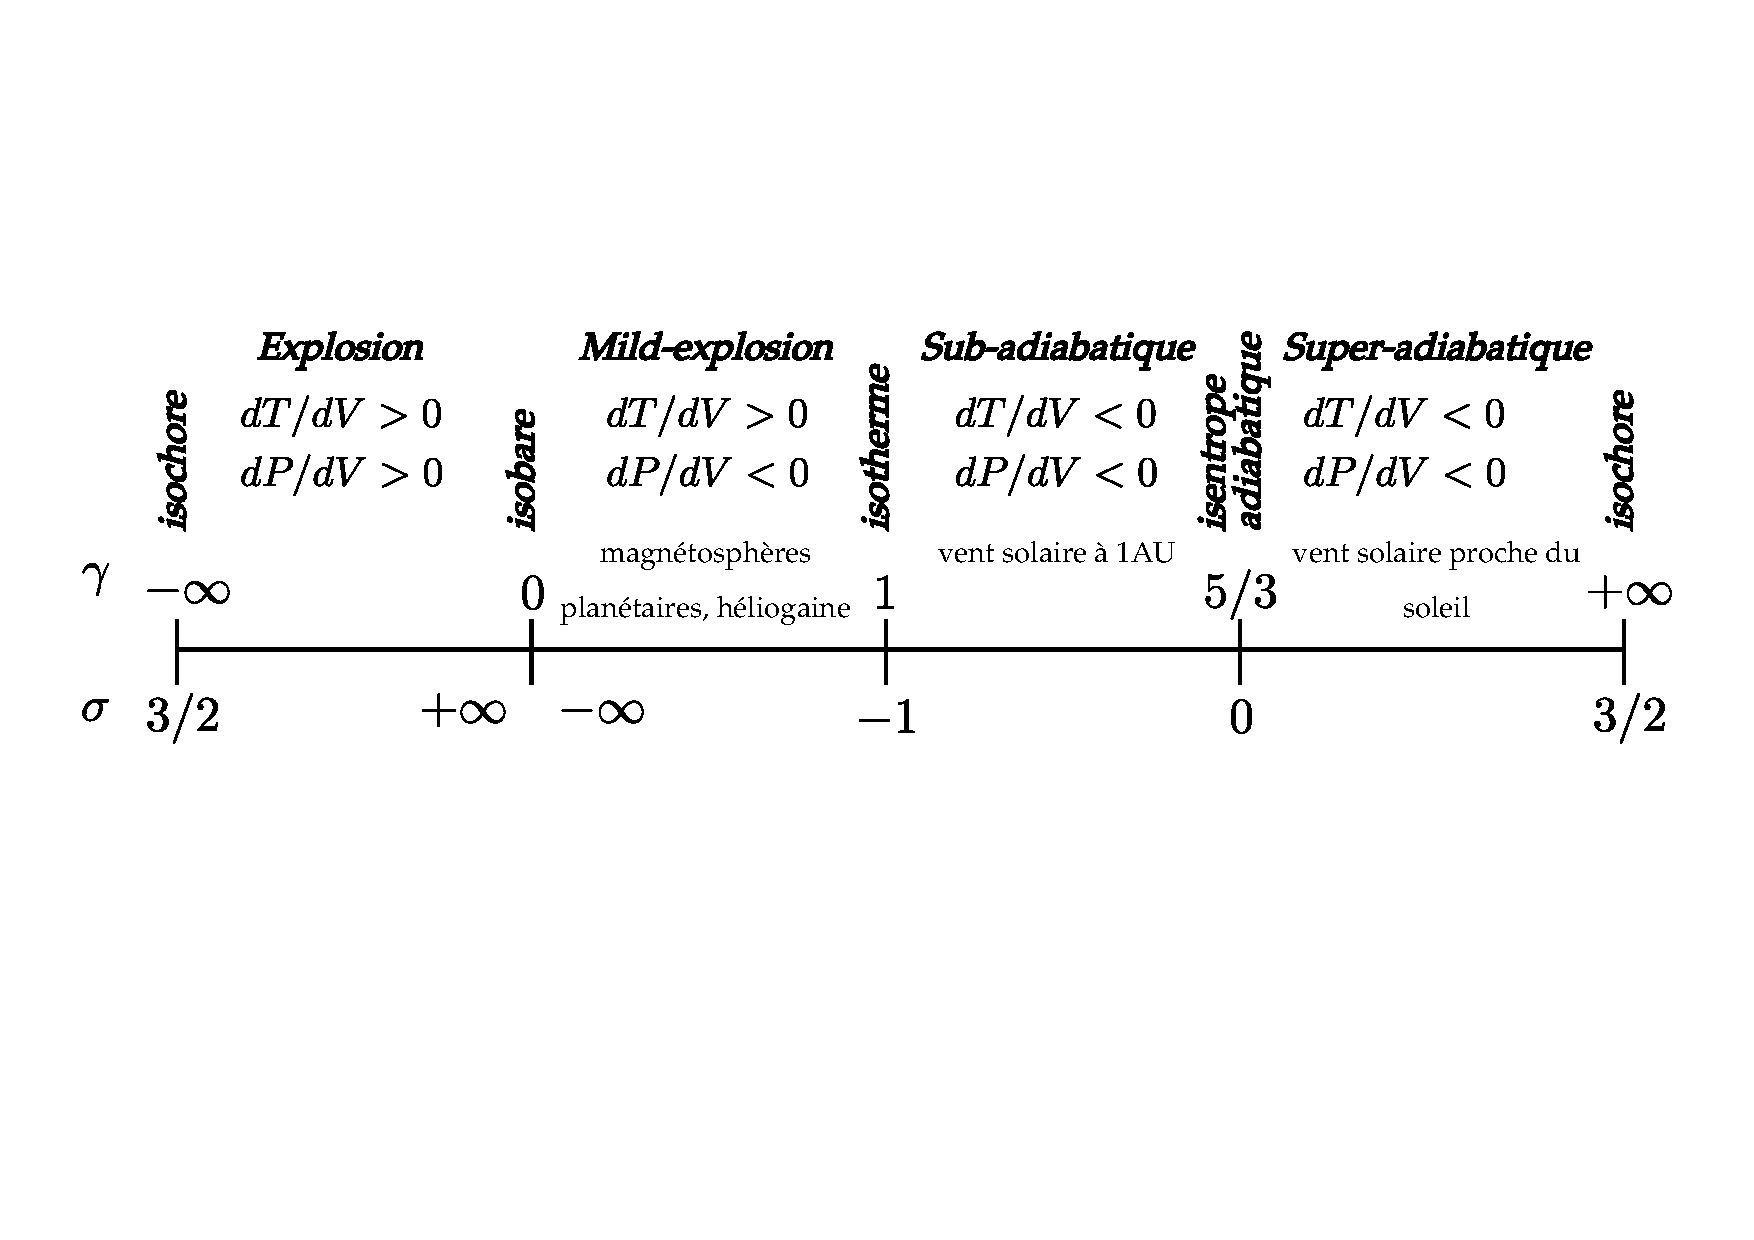
\includegraphics[width=0.9\linewidth,trim=1cm 8cm 1cm 5.5cm, clip=true]{./Part_1/images/schema_thermo.pdf}
\caption{Transformations thermodynamiques et intervalles en fonction du $\gamma$ du milieu [\cite{livadiotis_non-equilibrium_2012}] et du $\sigma$ [\cite{borel_thermodynamique_2005}], exemple de plasmas spatiaux [\cite{livadiotis_long-term_2018}]. Adiabatique et isentrope y sont confondus dans le cas réversible.}
\label{fig:schema_thermo}
\end{figure}

Dans le premier principe \eqref{eq:thermo_L1} et l'équation d'énergie interne \eqref{eq:thermo_u}, l'utilisation de $\sigma$ permet d'écrire : 
\begin{eqnarray}
\label{eq:thermo_sig_L1}    du &=& \dj \mathcal{Q} + \dj \mathcal{W} = \left(K+1\right) \dj \mathcal{W} = \left(\sigma \gamma + 1\right) \dj \mathcal{W} ,\\
\label{eq:thermo_sig_u}    d_t\left(\rho u\right) &=& -\left[\left(\sigma \gamma + 1\right) p + \rho u\right] \nabla \cdot \boldsymbol{v} ,\\
 \label{eq:thermo_sig_q}   &\Rightarrow& \nabla \cdot \boldsymbol{q} = -\rho T d_t s = \sigma \gamma p \nabla \cdot \boldsymbol{v}.
\end{eqnarray}
D'un autre côté, la relation entre $p$ et $V$ peut s'écrire $p \propto \rho^{\gamma}$. Cela donne l'équation : 
\begin{eqnarray}
 \label{eq:thermo_sig_p}   d_t p &=& -\gamma p \nabla \cdot \boldsymbol{v}.
\end{eqnarray}
Cette équation est compatible avec l'équation de pression du modèle fluide \eqref{eq:model_cpi_p} si :
\begin{eqnarray}
\label{eq:thermo_sig_gq}     \left(\frac{5}{3} -\gamma\right) p \nabla \cdot \boldsymbol{v} = -\frac{2}{3} \nabla \cdot \boldsymbol{q} 
\label{eq:thermo_sig_g}     &\Rightarrow& \left(\frac{5}{3} +\left(\frac{2}{3}\sigma-1\right)\gamma\right) p \nabla \cdot \boldsymbol{v} = 0 .
\end{eqnarray}
Par ces relations, on remarque que l'hypothèse polytrope peut nous permettre de fermer le modèle fluide au niveau du troisième moment $\boldsymbol{q}$ en injectant \eqref{eq:thermo_sig_q} dans l'équation de $p$ \eqref{eq:model_cpi_p}, ou au niveau du deuxième, $p$, en utilisant $\gamma$ et en injectant $p \propto \rho^{\gamma}$ dans \eqref{eq:model_cpi_v}\footnote{Usuellement, comme on cherche à fermer le modèle aussi tôt que possible, on ferme au niveau du deuxième moment. L'information sur le flux de chaleur est alors perdue d'où la confusion entre isentrope et polytrope.}. L'hypothèse adiabatique, isentrope si réversible, $\gamma=\gamma_a$ et $\nabla \cdot \boldsymbol{q}=0$, est retrouvée dans l'évolution fluide de $p$ si l'on se place dans le cadre d'un gaz parfait monoatomique $\gamma_a = 5/3$ d'après \eqref{eq:thermo_sig_gq}. Dans le cas isotherme, on retrouve dans \eqref{eq:thermo_sig_gq} ou \eqref{eq:thermo_sig_L1}, $\dj \mathcal{W} = - \dj \mathcal{Q}$, c'est-à-dire $du = 0$. En effet, la variation d'énergie interne d'un gaz parfait ne dépendant que de la température, ne peut qu'être nulle sous l'hypothèse d'isothermie. Les cas isochore (ou incompressible) et isobare sont plus délicats. Dans le cas isochore, le produit $\gamma \nabla \cdot \boldsymbol{v}$ qui apparaît dans toutes les expressions de \eqref{eq:thermo_sig_L1} à \eqref{eq:thermo_sig_g}, tend vers $\infty \times 0$. Dans le cas isobare, $\infty \times 0$ apparaît dès que $\sigma \gamma$ est présent dans l'équation. Ces limites du cas polytrope sont donc problématiques dans la définition de $u$. Elles doivent être traitées indépendamment. Dans le cas isochore, $\dj \mathcal{W} = 0$ et l'énergie interne ($d_t u + \nabla \cdot \boldsymbol{q} = 0 $) n'échange plus avec les énergies cinétique et magnétique. L'hypothèse isobare, quant à elle, ferme le système fluide au niveau de l'équation \eqref{eq:model_cpi_v}. L'équation d'énergie interne est alors  $\partial_t u + \nabla \cdot \left(u \boldsymbol{v} + \boldsymbol{q} + p_0 \boldsymbol{v}\right) = 0 $. Pour ces deux fermetures, l'énergie interne est conservée\footnote{La cascade d'énergie cinétique et magnétique peut alors être traitée indépendamment de celle d'énergie interne.  Cela a été fait dans le chapitre \ref{ch-11} dans le cadre incompressible.}.

Dans le cadre de la fermeture polytrope : $p = \frac{c_s^2}{\gamma} \rho$, avec $c^2_s = \frac{\partial p}{\partial \rho} \propto \rho^{\gamma-1}$ le carré de la vitesse thermique. Pour ce qui est de la variation d'énergie interne spécifique, elle devient :
\begin{eqnarray}
\label{eq:thermo_pol_du} d u &=& \left(\sigma \gamma+1\right) \frac{p}{\rho^2} d \rho =  \left(\sigma \gamma+1\right) \frac{p}{\rho^{\gamma}} \rho^{\gamma -2} d \rho \\
&=& \left\{ \begin{array}{lcl} \frac{\sigma \gamma+1}{\gamma-1} \frac{p}{\rho^{\gamma}} d\left( \rho^{\gamma-1} \right)  &\textrm{ si }&  \gamma \neq 1\\
\left(\sigma+1\right) \frac{p}{\rho} d \left(\ln{\rho}\right)  &\textrm{ si }&  \gamma = 1
\end{array} \right. .
\end{eqnarray}
Et par intégration :
\begin{eqnarray}
\label{eq:thermo_pol_u} u - u_I &=& \left\{ \begin{array}{lclcl} \frac{\sigma \gamma+1 }{\gamma-1} \frac{p}{\rho^{\gamma}} \left(\rho^{\gamma-1} - \rho_I^{\gamma-1}\right) &=& \frac{\sigma \gamma+1 }{\gamma-1} \frac{c_s^2}{\gamma} \left(1 - \left(\frac{\rho_I}{\rho}\right)^{\gamma-1}\right)  & \textrm{ si } & \gamma \neq 1\\
   \left(\sigma+1\right) \frac{p}{\rho} \ln \frac{\rho}{\rho_I} &=& \left(\sigma+1\right) c_s^2 \ln \frac{\rho}{\rho_I} &\textrm{ si }&  \gamma = 1 
   \end{array} \right. ,
\end{eqnarray} 
en notant $u_I$ et $\rho_I$ les constantes d'intégrations.
Dans le cas particulier de la fermeture isotherme : $\gamma = 1$, $\sigma = -1$, $p = c^2_s \rho$ avec $c_s$ constante et $du = 0$. 

\section{Thermodynamique et turbulence} \label{sec-112bis}

La cascade turbulente pourrait être, dans les plasmas spatiaux peu collisionnels, une réponse au problème du chauffage. En définissant le chauffage comme la variation de température et sachant que pour un gaz parfait, l'énergie interne ne dépend que de la température\footnote{Dans un gaz parfait, on suppose que les particules n'interagissent pas entre elles, donc qu'elles soient éloignées ou proches n'influera pas sur leur énergie individuelle. Par conséquent, l'énergie interne est indépendante de la densité. Cependant, la densité d'énergie interne dépendra de $\rho$ et $T$.}. Il est facile de définir le chauffage comme tout transfert d'énergie vers l'énergie interne, appelée aussi énergie thermique [\cite{cassak_pressure-strain_2022}]. Le terme de pression dans l'équation \eqref{eq:model_cpi_v} s'interprète alors comme les termes visqueux et résistifs abordés dans le Chapitre \ref{ch-11}, c'est-à-dire comme un terme "dissipatif". Mais, ce serait oublier que la cascade turbulente permet de faire le lien entre les grandes échelles, MHD où la validité de l'hypothèse de gaz parfait est cohérente puisque l'on néglige les interactions entre ions et électrons, et les petites échelles, cinétiques, où les interactions commencent à apparaître à travers le champ électromagnétique. Il manque donc un ingrédient à la définition du chauffage comme un transfert d'énergie vers l'énergie interne. Si l'on regarde la dissipation visqueuse ou résistive, elle vient réduire l'énergie du système, mais elle apparaît aussi dans l'équation d'entropie [\cite{eyink_cascades_2018}]. Chauffer ainsi va donc venir augmenter l'entropie du plasma. {\bf La définition du chauffage adaptée à l'étude de la turbulence est donc celle d'un transfert énergétique avec l'énergie interne impactant l'entropie. Le taux de cascade doit donc prendre en compte l'énergie étant transférée isentropiquement à l'énergie interne.}

Cette définition du chauffage justifie l'hypothèse proposée par [\cite{galtier_exact_2011}] que seul le terme de travail $\dj \mathcal{W}$ de l'énergie interne affecte la cascade dans la zone inertielle. Cette hypothèse revient à supposer une zone inertielle isentrope telle que $\sigma = 0$. Si le système global est fermé tel que $\gamma \neq \gamma_a$, le terme de chaleur $\dj \mathcal{Q}$ jouera un rôle aux autres échelles afin que les relations thermodynamiques soient respectées dans le système global. La fermeture considérée par [\cite{galtier_exact_2011}] est la fermeture isotherme qui dans l'hypothèse d'une zone inertielle isentrope implique :  $\gamma = 1$, $\sigma = 0$, $p = c^2_s \rho$ avec $c_s$ constante et $du = \dj \mathcal{W} \Rightarrow u-u_I = \frac{p}{\rho} \ln \frac{\rho}{\rho_I} $. On appellera cette fermeture, qui n'est valable que dans la zone inertielle, <<isentrope-isotherme>> afin d'expliciter la nuance existant entre l'isotherme basique tel que $du = 0$ et l'isotherme étudié dans le cadre d'une cascade isentrope. En suivant cette logique, je me suis intéressée dans [\cite{simon_general_2021}] à la fermeture <<isentrope-polytrope>> telle que $\sigma = 0$,  $p = \frac{c_s^2}{\gamma} \rho^{\gamma}$ et 
\begin{eqnarray}
\label{eq:thermo_ipol_u} u - u_I &=& \left\{ \begin{array}{lclcl} \frac{1 }{\gamma-1} \frac{p}{\rho^{\gamma}} \left(\rho^{\gamma-1} - \rho_I^{\gamma-1}\right) &=& \frac{+1 }{\gamma-1} \frac{c_s^2}{\gamma} \left(1 - \left(\frac{\rho_I}{\rho}\right)^{\gamma-1}\right)  & \textrm{ si } & \gamma \neq 1\\
    \frac{p}{\rho} \ln \frac{\rho}{\rho_I} &=&  c_s^2 \ln \frac{\rho}{\rho_I} &\textrm{ si }&  \gamma = 1 
   \end{array} \right. .
\end{eqnarray} 
Dans l'usage des formes explicites de l'énergie interne dans les calculs de lois exactes avec l'hypothèse polytrope, les constantes sont souvent annulées entre elles. Par exemple, dans le cas <<isentrope-polytrope>>, \cite{banerjee_kolmogorov-like_2014} considère comme forme explicite de l'énergie interne $ \rho u = \frac{1}{\left(\gamma-1\right)} p $. Contrairement à ce travail, nous avons choisi de maintenir une forme de compatibilité avec la fermeture <<isentrope-isotherme>> de \cite{galtier_exact_2011} (si $u = u_I$ alors $u = 0$) dans nos choix de constantes.

Sont résumés dans la \tabref{tab:fermetures}, les caractéristiques, dénominations et choix de constante des fermetures définies polytropiquement via $\sigma$ et $\gamma$ qui serviront par la suite. 
\begin{table}[!ht]
\begin{center}
\begin{tabular}{ c|c|c } 
Nom & Paramètres & Energie interne explicite\\
\hline
Polytrope (hors isotherme)  & $\{\sigma,\gamma \neq 1 \}$  & $ \frac{\sigma \gamma+1 }{\gamma-1} \frac{p}{\rho^{\gamma}} \left(\rho^{\gamma-1} - \rho_I^{\gamma-1}\right) $    \\
Isotherme  & $\{-1,1\}$ & $  u = 0$     \\
Isentrope-polytrope (hors isotherme) & $\{0,\gamma \neq 1\}$ & $ \frac{1 }{\gamma-1} \frac{p}{\rho^{\gamma}} \left(\rho^{\gamma-1} - \rho_I^{\gamma-1}\right)  $  \\
Isentrope-isotherme & $\{0,1\}$  & $ u = \frac{p}{\rho} \ln \frac{\rho}{\rho_I}$  \\
\end{tabular}
\end{center}
\caption{Fermetures et relations associées. La forme de l'énergie interne de l'isentrope-isotherme est calquée sur celle utilisée par \cite{galtier_exact_2011}. Les autres sont définies de telle sorte à maintenir une forme de compatibilité : si $u = u_I$ alors $u = 0$. Celle de l'isentrope-polytrope est donc légèrement différente de celle utilisée par \cite{banerjee_kolmogorov-like_2014}. $\frac{p}{\rho}$ peut aussi s'écrire $\frac{c_s^2}{\gamma}$ et $p \propto \rho^{\gamma}$. \label{tab:fermetures}}
\end{table}

\cite{aluie_conservative_2012} observent en détail la cascade d'énergie cinétique et magnétique dans différentes simulations subsoniques à transoniques. Le transfert cinétique-interne via la pression semble n'avoir lieu qu'à grande échelle dans une zone qu'ils appellent <<zone de conversion>>, à plus petites échelles cette contribution reste constante. Ils en déduisent un découplage des cascades d'énergie cinétique et d'énergie interne et l'existence d'une zone inertielle cinétique. \cite{eyink_cascades_2018} déduisent aussi, analytiquement, un effet à grande échelle de la pression qui permettrait d'alimenter des structures cohérentes et de réduire l'entropie à grande échelle. Cela induirait une cascade inverse d'entropie vers les grandes échelles et un équilibre s'établirait entre les cascades d'énergie totale et d'entropie. Aucun de ces résultats ne prouve que l'énergie interne ne cascade pas. Ne pas la prendre en compte dans l'estimation du taux de chauffage comme le propose \cite{hellinger_von_2018} est donc hasardeux et n'est justifiable que dans le cas subsonique où sa contribution semble mineure [\cite{andres_energy_2018,ferrand_compressible_2020}] ou à des échelles plus faibles que celle où l'impact de la pression semble majeur [\cite{aluie_conservative_2012}]. Etudier la cascade compressible dans une zone inertielle où la pression ne transférerait pas d'énergie vers l'énergie interne, c'est à dire $\nabla p = 0$ dans l'équation \eqref{eq:lin_cpi_v}, correspondrait à regarder une zone inertielle isobare. Au vu des observations, cela ne semble pas physiquement absurde, mais étant intéressés par l'impact de la pression sur la cascade turbulente totale, cette hypothèse réductrice n'a pas retenu notre intérêt. 


\section{Propriétés linéaires de la \ac{MHD} compressible}
\label{sec-123}

Dans le cadre de l'obtention d'une relation de dispersion compressible, on fermera le système avec la fermeture polytrope pour rester dans le cas le plus général possible. Ainsi, on utilise le système d'équations : 
\begin{eqnarray}
\label{eq:lin_cpi_r}\partial_t \rho + \nabla \cdot \left(\rho \boldsymbol{v}\right) &=& 0,\\
\label{eq:lin_cpi_v}\partial_t \left(\rho \boldsymbol{v}\right) + \nabla \cdot \left(\rho \boldsymbol{v}\boldsymbol{v} - \rho \boldsymbol{v_A}\boldsymbol{v_A}\right) +  \nabla p_*  &=& 0 \label{eq:model_1}, \\
\label{eq:lin_cpi_b}\partial_t \boldsymbol{v_A} -  \nabla \cdot \left(\boldsymbol{v_A}\boldsymbol{v} - \boldsymbol{v}\boldsymbol{v_A}\right) +  \boldsymbol{v}  \nabla \cdot \boldsymbol{v_A} -  \frac{\boldsymbol{v_A}}{2}  \nabla \cdot \boldsymbol{v} &=& 0 ,
\end{eqnarray}
fermé par $p\propto \rho^{\gamma}$. 
 
L'application de la méthode de linéarisation présentée dans le Chapitre \ref{ch-11} nous donne l'équation de dispersion suivante :
\begin{equation}
    \begin{pmatrix}
\label{eq:lin_cpi_eqdis}    \frac{\omega^2}{k^2_{\parallel} v^2_{A0}} - \left(1+\frac{\gamma}{2} \beta_0\right)  \frac{k^2_{\perp}}{k^2_{\parallel}} - 1 & 0 & - \frac{\gamma}{2} \beta_0  \frac{k_{\perp}}{k_{\parallel}} \\
    0 & \frac{\omega^2}{k^2_{\parallel} v^2_{A0}} - 1  & 0 \\
     - \frac{\gamma}{2} \beta_0  \frac{k_{\perp}}{k_{\parallel}}  & 0 &\frac{\omega^2}{k^2_{\parallel} v^2_{A0}} -  \frac{\gamma}{2} \beta_0   
    \end{pmatrix} 
    \cdot \begin{pmatrix}
    v^{1}_x \\ v^{1}_y \\ v^{1}_z
    \end{pmatrix} = 0
\end{equation}
avec $\beta_0 = \frac{2p_0}{\rho_0 v^2_{A0}}$ le paramètre $\beta$ linéarisé du plasma. 
La relation de dispersion est donnée par l'annulation du déterminant de la matrice, c'est-à-dire, :
\begin{eqnarray}
 \label{eq:lin_cpi_disp}   0 = \left(\frac{\omega^2}{k^2_{\parallel} v^2_{A0}} - 1 \right)\left(\frac{\omega^2}{k^2 v^2_{A0}} - \frac{1}{2} \left(1+ \frac{\gamma}{2} \beta_0 \pm \sqrt{\Delta}\right)\right)
\end{eqnarray}
avec $\Delta = \left(1- \frac{\gamma}{2} \beta_0\right)^2 +2 \gamma \beta_0\sin^2\theta  = \left(1+ \frac{\gamma}{2} \beta_0\right)^2 -2 \gamma \beta_0\cos^2\theta$ en notant $\theta$ l'angle entre $\boldsymbol{k}$ et $\boldsymbol{e_z}$. La première racine correspond au mode d'Alfvén incompressible et les deux autres aux modes magnétosonores rapide ($+$) et lent ($-$). Ces modes sont stables ($\omega$ est réel), puisque $\Delta > 0$ et $\frac{1}{2} \left(1+ \frac{\gamma}{2} \beta_0 \pm \sqrt{\Delta}\right)>0$. 

Ces modes et leur version cinétique influencent le développement de la cascade turbulente en interagissant les uns avec les autres [\cite{cho_compressible_2003,sharma_nonlinear_2011,andres_interplay_2017,brodiano_spatiotemporal_2021,galtier_fast_2023}]. Dans le vent solaire, quasi-incompressible, le mode d'Alfvén et la cascade associée sont dominants. Cependant, les simulations et des filtrages de spectres relevés dans la magnétogaine ou la couronne solaire montrent des spectres de types turbulents pour les ondes magnétosoniques. Les simulations sont des outils très utilisés pour essayer de comprendre la répartition des rôles des différents modes [\cite{brodiano_spatiotemporal_2021}] mais l'universalité des résultats est questionnable, les résultats étant dépendants du forçage (Alfvénique ou non) initiant la cascade.  

\newpage
\section{Synthèse sur le modèle compressible avec pression isotrope}
\label{synt-12}
\fcolorbox{blue}{white}{\begin{minipage}[c]{\linewidth}
\paragraph{Modèle : } 
\begin{eqnarray}
\label{eq:synth_cpi_r} \partial_t \rho + \nabla \cdot \left(\rho \boldsymbol{v}\right) &=& 0 ,\\
\label{eq:synth_cpi_v}  \partial_t \left(\rho \boldsymbol{v}\right) + \nabla \cdot \left(\rho \boldsymbol{v}\boldsymbol{v} - \rho \boldsymbol{v_A}\boldsymbol{v_A}\right) +  \nabla p_*  &=& 0  ,\\
\label{eq:synth_cpi_b} \partial_t \boldsymbol{v_A} -  \nabla \cdot \left(\boldsymbol{v_A}\boldsymbol{v} - \boldsymbol{v}\boldsymbol{v_A}\right) +  \boldsymbol{v}  \nabla \cdot \boldsymbol{v_A} -  \frac{\boldsymbol{v_A}}{2}  \nabla \cdot \boldsymbol{v} &=& 0 , \\
\label{eq:synth_cpi_cb} \boldsymbol{v_A}\cdot \nabla  \rho  + 2\rho \nabla \cdot \boldsymbol{v_A}  &=& 0.
\end{eqnarray}

\paragraph{Fermetures écrites dans le cadre général polytrope et formes explicites de l'énergie interne spécifique considérées (telles que $u_I =u\left(\rho = \rho_I\right) =  0$) : } 
\begin{equation}
    \frac{p}{\rho} = \frac{c_s^2}{\gamma}, \quad c_s^2 \propto \rho^{\gamma-1}, \quad \sigma = \frac{\nabla \cdot \boldsymbol{q}}{\gamma p\nabla \cdot \boldsymbol{v}} ,\nonumber
\end{equation}
\begin{itemize}
    \item cas polytrope hors isotherme : $u = \frac{\sigma \gamma+1 }{\gamma-1} \frac{p}{\rho^{\gamma}} \left(\rho^{\gamma-1} - \rho_I^{\gamma-1}\right)$,
    \item cas isotherme : $\sigma = -1$, $\gamma = 1$, $u = 0$ et $c_s$ constants,
    \item cas isentrope-polytrope hors isotherme : $\sigma = 0$ et  $u = \frac{ \gamma+1 }{\gamma-1} \frac{p}{\rho^{\gamma}} \left(\rho^{\gamma-1} - \rho_I^{\gamma-1}\right) $,
    \item cas isentrope-isotherme  : $\sigma = 0$, $\gamma = 1$, $c_s$ constant et $u = c_s^2 \ln{\frac{\rho}{\rho_I}}$.
\end{itemize}

\paragraph{Equation d'énergie interne :} 
\begin{eqnarray}
\label{eq:synth_cpi_u} &\text{Formulation générale : }& \partial_t \left(\rho u\right) +\nabla \cdot \left(\rho u \boldsymbol{v} + \boldsymbol{q}\right)   = - p \nabla \cdot \boldsymbol{v} ,\\
\label{eq:synth_L1_du} &\text{Premier principe thermo : }& du =  \dj \mathcal{Q} + \dj \mathcal{W} = Tds + \frac{p}{\rho^2} d\rho , \\
\label{eq:synth_L1_u} &\text{Formulation thermo : }& \partial_t \left(\rho u\right) +\nabla \cdot \left(\rho u \boldsymbol{v}\right) - \rho T d_t s  = - p \nabla \cdot \boldsymbol{v}, \\
\label{eq:synth_L1_compu} &\Rightarrow \text{ Compatibilité : }& \nabla \cdot \boldsymbol{q} =  - \rho T d_t s , \\
\label{eq:synth_pol_u} &\text{Formulation polytrope : }& \partial_t \left(\rho u\right) +\nabla \cdot \left(\rho u \boldsymbol{v}\right)   = - \left(\sigma \gamma + 1 \right)p \nabla \cdot \boldsymbol{v} .
\end{eqnarray}

\paragraph{Equation de pression : }
\begin{eqnarray}
\label{eq:synth_cpi_p} &\text{Modèle fluide non fermé : }& \partial_t p + \nabla \cdot \left(  p\boldsymbol{v} + \frac{2}{3}\boldsymbol{q}\right) + \frac{2}{3} p \nabla \cdot \boldsymbol{v}  = 0 ,\\
\label{eq:synth_pol_p} &\text{Fermeture polytrope ($p \propto \rho^{\gamma}$) : }& \partial_t p + \boldsymbol{v} \cdot \nabla p - \gamma p \nabla \cdot \boldsymbol{v} = 0 ,\\
\label{eq:synth_cpi_comp} &\Rightarrow \text{ Compatibilité : }& \left(\frac{5}{3} + \left(\frac{2}{3}\sigma -1\right) \gamma\right)\nabla \cdot \boldsymbol{v} = 0 .
\end{eqnarray}

\end{minipage}}

\fcolorbox{blue}{white}{\begin{minipage}[c]{\linewidth}
\paragraph{Relation de dispersion linéaire : }
\begin{eqnarray}
 0 = \left(\frac{\omega^2}{k^2_{\parallel} v^2_{A0}} - 1 \right)\left(\frac{\omega^2}{k^2 v^2_{A0}} - \frac{1}{2} \left(1+ \frac{\gamma}{2} \beta_0 \pm \sqrt{\left(1- \frac{\gamma}{2} \beta_0\right)^2 +2 \gamma \beta_0\sin^2\theta}\right)\right) .
\end{eqnarray}
La première racine correspond au mode d'Alfvén similaire à celui obtenu en incompressible et les deux autres aux modes magnétosonores rapide ($+$) et lent ($-$). 
\end{minipage}}


\chapitre{Décrire la cascade compressible}{ch-13}
\chapter{Décrire la cascade compressible}
\renewcommand\partie{\Partie\ Chapitre \thechapter}
\label{ch-13}

%\medskip
\minitoc  

\bigskip

La variation du résultat de l'estimation d'un indice polytropique dans différents types de plasmas spatiaux (voir \figref{fig:schema_thermo}, [\cite{livadiotis_thermodynamic_2018}]) vient motiver la dérivation d'une loi exacte polytrope pour étudier la cascade d'énergie totale dans ces milieux. L'objectif initial du travail présenté dans cette partie et dont la contribution originale analytique est introduite dans ce chapitre, était de dériver une loi exacte \ac{MHD} polytrope, une extension des modèles \ac{MHD} isothermes [\cite{banerjee_exact_2013,andres_alternative_2017,andres_exact_2018,ferrand_compact_2021}] et \ac{HD} polytrope [\cite{banerjee_kolmogorov-like_2014}] existants. La cascade y est décrite similairement à celle décrite par \cite{galtier_exact_2011} (cas \ac{HD} isotherme). Suite à la discussion sur les fermetures thermodynamiques résumée dans le Chapitre \ref{ch-12}, on peut dire que, dans ces articles, elle est supposée isentrope dans la zone inertielle. L'hypothèse d'une fermeture polytrope (resp. isotherme) avec une zone inertielle isentrope revient à la fermeture "isentrope-polytrope" (resp. isentrope-isotherme) discutée au Chapitre \ref{ch-12}.

La méthode de calcul envisagée pour atteindre l'objectif initial a en réalité permis d'obtenir une loi exacte générale valable pour toutes les fermetures du système tant que l'isentropie est imposée dans la zone inertielle. 
Ce travail dont l'application à la fermeture "isentrope-polytrope" répond à l'objectif initial est présenté dans la section \ref{sec-131}. 
Dans la section \ref{sec-132}, on détaillera l'impact des fermetures sur une autre formulation de la loi qui a émergée du travail de relaxation de l'hypothèse d'isotropie de pression qui sera présenté dans le Chapitre \ref{ch-21}. 
Bien après avoir atteint l'objectif initial, on s'est posé la question de l'impact du flux de chaleur (a priori attendu en dehors de la zone inertielle) et on l'a pris en compte dans la loi \acs{KHM} qui, ainsi, a réellement pris une dimension générale. Notre loi a alors adopté une troisième formulation qui sera présentée dans la section \ref{sec-133}. Des applications isobare, isotherme et polytrope y seront abordées en tant qu'exemples d'application clôturant ce travail de généralisation.

\section{Dérivation d'une loi exacte compressible générale pour décrire un écoulement turbulent polytrope}
\label{sec-131}

La méthode utilisée ici pour dériver une loi exacte compressible correspond à celle détaillée dans le cas incompressible et résumée dans la section \ref{synt-11}. La première étape est de définir une fonction de corrélation. La pluralité de possibilités est plus importante que dans le cas incompressible puisque cette fois la compression ($\rho \neq 0$) impacte les densités d'énergie : $E_{tot} = \frac{1}{2} \rho \boldsymbol{v}^2 + \frac{1}{2} \rho \boldsymbol{v_A}^2 + \rho u $. Pour l'énergie cinétique, la volonté de considérer une forme de type auto-corrélation, a inspiré des études \ac{HD} et \ac{MHD} considérant sa racine-carré en $\sqrt{\rho} \boldsymbol{v} $ [\cite{hellinger_spectral_2021}] tandis que d'autres ont privilégié le sens physique de la quantité de mouvement $\rho \boldsymbol{v}$ (ex : \cite{galtier_exact_2011}). Pour l'énergie magnétique, la question est la même : $\boldsymbol{B}$ [\cite{ferrand_compact_2021}] ou $\rho \boldsymbol{v_A}$ [\cite{andres_alternative_2017}] ? Et pour l'énergie interne, les choix présents dans la littérature ont été en partie orientés suivant le type de fermeture : dans le cas polytrope par exemple, la forme explicite de l'énergie interne spécifique peut s'écrire tel que le carré de la vitesse thermique, d'où $\rho \sqrt{u}$ [\cite{banerjee_kolmogorov-like_2014}] ou $\sqrt{\rho u}$ alors que, dans le cas isotherme [\cite{galtier_exact_2011}], le choix était plutôt orienté vers la conservation de son intégrité et de prendre $\rho$ en un point et $u$ en un autre. Trois possibilités ont été envisagées pour chaque type d'énergie (dont la forme est ici généralisée en $E_\mathcal{X} = \rho X^2$) : 
\begin{itemize}
    \item l'auto-corrélation : $\mathcal{R_{X}}_1 = \left<\sqrt{\rho'} X' \cdot \sqrt{\rho} X \right>$ de fonction incrémentale associée :  $\mathcal{S_{X}}_1 = \left<\left(\delta \left(\sqrt{\rho} X\right)\right)^2\right>$ puisque $\mathcal{S_{X}}_1 = 2\left<E_\mathcal{X}\right> - 2\mathcal{R_{X}}_1 $
    \item la moyenne de densité : $\mathcal{R_{X}}_2 = \frac{1}{2}\left< \left(\rho'+\rho\right) X' \cdot X \right>$ de fonction incrémentale associée :  $\mathcal{S_{X}}_2 = \left<\delta \left(\rho X\right) \cdot \delta X \right>$ 
    \item la corrélation avec la densité : $\mathcal{R_{X}}_3 = \frac{1}{2}\left< \rho' X^2 + \rho X'{}^2\right> $ de fonction incrémentale associée :  $\mathcal{S_{X}}_3 = \left<\delta \rho  \delta X^2 \right>$ 
\end{itemize}
Il s'avère qu'utiliser des formes prenant en compte des racines carrées a tendance à compliquer le calcul et le résultat. Les formes finalement choisies sont donc : $\mathcal{R}_{c} = \mathcal{R}_{c2} = \left<\frac{1}{4} \left(\rho'+\rho\right) \boldsymbol{v'} \cdot  \boldsymbol{v} \right>$, $\mathcal{R}_{m} = \mathcal{R}_{m2} = \left<\frac{1}{4} \left(\rho'+\rho\right) \boldsymbol{v'_A} \cdot  \boldsymbol{v_A} \right>$ et $\mathcal{R}_{u} = \mathcal{R}_{u3} = \frac{1}{2}\left< \rho' u + \rho u'\right> $. Ce choix concorde avec celui de \cite{andres_energy_2018} dont les résultats de simulation permettront l'étude dans les données in-situ du Chapitre \ref{ch-14} et serviront de base de comparaison afin de valider les résultats de simulations présentés dans la Partie \ref{part_3}.

Pour ce qui est du modèle considéré, la première idée était d'appliquer la méthode de calcul des lois exactes sur le modèle fermé par l'hypothèse $p \propto \rho^{\gamma}$, dans la lignée des dérivations compressibles effectuées par exemple par \cite{galtier_exact_2011} et \cite{andres_alternative_2017}. Mais il s'est avéré qu'un autre choix plus judicieux existait. En effet, comme pour obtenir l'équation d'énergie totale \eqref{eq:model_cpi_e}, nous pouvons obtenir une loi exacte <<générale>> en utilisant l'équation de densité d'énergie interne \eqref{eq:synth_cpi_u} et sans expliciter la forme de $p$ ni celle de $u$. En première approximation, l'hypothèse isentrope qui implique $\nabla \cdot \boldsymbol{q} = 0$ via l'équation de compatibilité \eqref{eq:synth_L1_compu}, a d'abord été posée. Ce travail fait partie des résultats publiés dans \cite{simon_general_2021}. La loi \acs{KHM} générale qui y est obtenue n'est alors valable que dans la zone inertielle où l'hypothèse isentrope est supposée effective et ne sert que d'étape de calcul vers une loi \acs{K41}. Dans une volonté de donner un résultat pour la loi \acs{KHM} générale valable pour toutes les échelles, nous prendrons en compte $\nabla \cdot \boldsymbol{q}$ dans cette section, mais nous garderons sa contribution brute, sans travail analytique en accord avec le cheminement chronologique voulu pour ce chapitre. 

Les équations considérées sont celles de densité de masse \eqref{eq:synth_cpi_r}, vitesse  \eqref{eq:synth_cpi_v}, induction \eqref{eq:synth_cpi_b} et énergie interne  \eqref{eq:synth_cpi_u} avec des termes de forçage et de dissipation définis comme dans le cas incompressible (voir \eqref{eq:synth_inc_v} et \eqref{eq:synth_inc_b}). Ainsi :
\begin{eqnarray}
\label{eq:turb_cpi_r} \partial_t \rho &=& - \nabla \cdot \left(\rho \boldsymbol{v}\right), \\
\label{eq:turb_cpi_v}\partial_t  \boldsymbol{v} &=&- \nabla \cdot \left(\boldsymbol{v}\boldsymbol{v}\right) + \boldsymbol{v} \nabla \cdot \boldsymbol{v}  + \frac{1}{\rho} \nabla \cdot \left(\rho \boldsymbol{v_A}\boldsymbol{v_A}\right) - \frac{1}{\rho}  \nabla p_*  + \boldsymbol{f_c} + \boldsymbol{d_c} ,\\
\label{eq:turb_cpi_b}\partial_t \boldsymbol{v_A} &=&   \nabla \cdot \left(\boldsymbol{v_A}\boldsymbol{v} - \boldsymbol{v}\boldsymbol{v_A}\right) -  \boldsymbol{v}  \nabla \cdot \boldsymbol{v_A} +  \frac{\boldsymbol{v_A}}{2}  \nabla \cdot \boldsymbol{v} + \boldsymbol{f_m} + \boldsymbol{d_m} ,\\
\label{eq:turb_cpi_u}\partial_t u &=& - \nabla \cdot \left(u \boldsymbol{v}\right) + u  \nabla \cdot \boldsymbol{v} -\frac{1}{\rho} \nabla \cdot \boldsymbol{q}  - \frac{p}{\rho}  \nabla \cdot \boldsymbol{v} .
\end{eqnarray}
\eqref{eq:turb_cpi_v} et \eqref{eq:turb_cpi_b} peuvent aussi s'écrire en prenant en compte \eqref{eq:turb_cpi_r} :
\begin{eqnarray}
\label{eq:turb_cpi_v2}\partial_t  \left(\rho\boldsymbol{v}\right) &=&- \nabla \cdot \left(\rho \boldsymbol{v}\boldsymbol{v}\right)  + \nabla \cdot \left(\rho \boldsymbol{v_A}\boldsymbol{v_A}\right) -  \nabla p_*  + \rho \boldsymbol{f_c} + \rho\boldsymbol{d_c} ,\\
\label{eq:turb_cpi_b2}\partial_t \left(\rho\boldsymbol{v_A}\right) &=&   \nabla \cdot \left(\rho \boldsymbol{v_A}\boldsymbol{v} - \rho \boldsymbol{v}\boldsymbol{v_A}\right) +  \rho \boldsymbol{v}  \nabla \cdot \boldsymbol{v_A} - \frac{1}{2} \rho\boldsymbol{v_A} \nabla \cdot \boldsymbol{v} + \rho\boldsymbol{f_m} + \rho\boldsymbol{d_m}.
\end{eqnarray}

Si l'on regarde la forme des fonctions de corrélation incrémentales associées aux formes des fonctions choisies, on peut s'attendre à pouvoir identifier les fonctions de structure $\left<\delta \left(\rho\boldsymbol{v}\right) \cdot \delta \boldsymbol{v} \delta \boldsymbol{v}\right>$, $\left<\delta \left(\rho\boldsymbol{v_A}\right) \cdot \delta \boldsymbol{v_A} \delta \boldsymbol{v}\right>$ et $\left<\delta \rho \delta u \delta \boldsymbol{v}\right>$ et, similairement au cas incompressible, $\left<\delta \left(\rho\boldsymbol{v_A}\right) \cdot \delta \boldsymbol{v} \delta \boldsymbol{v_A}\right>$ ou $\left<\delta \left(\rho\boldsymbol{v}\right) \cdot \delta \boldsymbol{v_A} \delta \boldsymbol{v_A}\right>$. Le calcul de l'évolution temporelle des fonctions de corrélation pour chaque canal énergétique nous donne en effet : 
\begin{itemize}
    \item Canal d'énergie cinétique : $\mathcal{R}_{c} = \frac{1}{4}\left<\left(\rho'+\rho\right)\boldsymbol{v'} \cdot \boldsymbol{v}\right>$
\begin{eqnarray}
\label{eq:turb_cpi_Rc} 4\partial_t \mathcal{R}_{c} &=& \left<\partial_t \left(\rho' \boldsymbol{v'} \right)\cdot  \boldsymbol{v}  + \rho' \boldsymbol{v'} \cdot  \partial_t \boldsymbol{v} + \partial_t \left(\rho \boldsymbol{v} \right)\cdot  \boldsymbol{v'}  + \rho \boldsymbol{v} \cdot  \partial_t \boldsymbol{v'} \right>\nonumber \\
&=&\nabla_{\boldsymbol{\ell}} \cdot \left<\delta \left(\rho\boldsymbol{v}\right) \cdot \delta \boldsymbol{v} \delta \boldsymbol{v} -\left(\delta \left(\rho\boldsymbol{v_A}\right) \cdot \delta \boldsymbol{v} \delta \boldsymbol{v_A} + \delta \left(\rho\boldsymbol{v}\right) \cdot \delta \boldsymbol{v_A} \delta \boldsymbol{v_A} \right)\right>\nonumber \\
&&+ \nabla_{\boldsymbol{\ell}} \cdot \left<\rho' \boldsymbol{v'_A}\cdot  \boldsymbol{v} \boldsymbol{v_A} -\rho \boldsymbol{v_A}\cdot  \boldsymbol{v'} \boldsymbol{v'_A}-\rho' \boldsymbol{v'} \cdot\boldsymbol{v_A}\boldsymbol{v'_A} +  \rho  \boldsymbol{v} \cdot\boldsymbol{v'_A}\boldsymbol{v_A}\right> \nonumber\\
&& +\left< \rho \boldsymbol{v} \cdot \delta \boldsymbol{v} \nabla' \cdot \boldsymbol{v'} -\rho' \boldsymbol{v'} \cdot \delta \boldsymbol{v} \nabla \cdot \boldsymbol{v} +2 \rho' \boldsymbol{v'} \cdot \delta \boldsymbol{v_A}\nabla \cdot \boldsymbol{v_A} - 2\rho \boldsymbol{v} \cdot \delta \boldsymbol{v_A}\nabla' \cdot \boldsymbol{v'_A}\right> \nonumber\\
&&+  \nabla_{\boldsymbol{\ell}} \cdot \left< \left(1+\frac{\rho'}{\rho}\right)p_*  \boldsymbol{v'} -  \left(1+\frac{\rho}{\rho'}\right)p'_*  \boldsymbol{v} \right>- \left<\frac{\rho'}{\rho} p_*  \boldsymbol{v'} \cdot \frac{\nabla \rho}{\rho} + \frac{\rho}{\rho'} p'_*  \boldsymbol{v} \cdot \frac{\nabla' \rho'}{\rho'} \right>\nonumber\\
&&+  \left<\left(\rho' + \rho\right)\left(\boldsymbol{v} \cdot \boldsymbol{f'_c} + \boldsymbol{v'} \cdot \boldsymbol{f_c}\right) \right>+ \left<\left(\rho' + \rho\right)\left(\boldsymbol{v} \cdot \boldsymbol{d'_c} + \boldsymbol{v'} \cdot \boldsymbol{d_c}\right)\right> .
\end{eqnarray}
    \item Canal d'énergie magnétique : $\mathcal{R}_{m} = \frac{1}{4}\left<\left(\rho'+\rho\right)\boldsymbol{v'_A} \cdot \boldsymbol{v_A}\right> $
\begin{eqnarray}
\label{eq:turb_cpi_Rm} 4\partial_t \mathcal{R}_{m} &=& \left<\partial_t \left(\rho' \boldsymbol{v'_A} \right)\cdot  \boldsymbol{v_A}  + \rho' \boldsymbol{v'_A} \cdot  \partial_t \boldsymbol{v_A} + \partial_t \left(\rho \boldsymbol{v_A} \right)\cdot  \boldsymbol{v'_A}  + \rho \boldsymbol{v_A} \cdot  \partial_t \boldsymbol{v'_A} \right> \nonumber\\
&=&\nabla_{\boldsymbol{\ell}} \cdot \left<\delta \left(\rho\boldsymbol{v_A}\right) \cdot \delta \boldsymbol{v_A} \delta \boldsymbol{v} \right> + \left<\left(\rho \boldsymbol{v_A} \cdot \delta \boldsymbol{v_A} -\frac{1}{2} \left(\rho'+\rho\right) \boldsymbol{v'_A} \cdot \boldsymbol{v_A}\right)\nabla' \cdot \boldsymbol{v'}\right>\nonumber\\
&&-  \left<\left(\rho' \boldsymbol{v'_A} \cdot \delta \boldsymbol{v_A} + \frac{1}{2} \left(\rho'+\rho\right) \boldsymbol{v'_A} \cdot \boldsymbol{v_A}\right)\nabla \cdot \boldsymbol{v}\right>\\
&& + \left<\left( \rho' \boldsymbol{v'_A} \cdot \boldsymbol{v} - \rho \boldsymbol{v} \cdot \boldsymbol{v'_A}  \right)\nabla \cdot \boldsymbol{v_A} \right> + \left<\left(\rho' \boldsymbol{v'} \cdot \boldsymbol{v_A} -  \rho \boldsymbol{v_A} \cdot \boldsymbol{v'} \right)\nabla' \cdot \boldsymbol{v'_A} \right>\nonumber\\
&&-\nabla_{\boldsymbol{\ell}} \cdot \left< \rho' \boldsymbol{v'_A}\cdot  \boldsymbol{v} \boldsymbol{v_A} - \rho \boldsymbol{v_A}\cdot  \boldsymbol{v'} \boldsymbol{v'_A}-\rho' \boldsymbol{v'} \cdot\boldsymbol{v_A}\boldsymbol{v'_A} +  \rho  \boldsymbol{v} \cdot\boldsymbol{v'_A}\boldsymbol{v_A}\right> \nonumber\\
&&+  \left<\left(\rho' + \rho\right)\left(\boldsymbol{v_A} \cdot \boldsymbol{f'_m} + \boldsymbol{v'_A} \cdot \boldsymbol{f_m}\right) \right>+ \left<\left(\rho' + \rho\right)\left(\boldsymbol{v_A} \cdot \boldsymbol{d'_m} + \boldsymbol{v'_A} \cdot \boldsymbol{d_m}\right)\right> . \nonumber
\end{eqnarray}
 \item Canal d'énergie interne :  $\mathcal{R}_{u} = \frac{1}{2}\left<\rho' u+\rho u'\right> $
\begin{eqnarray}
\label{eq:turb_cpi_Ru} 2\partial_t \mathcal{R}_{u} &=& \left<\partial_t \left(\rho'\right) u  + \rho' \partial_t u + \partial_t \left(\rho\right) u' + \rho \partial_t u'\right> \nonumber\\
&=&\nabla_{\boldsymbol{\ell}} \cdot \left<\delta \rho  \delta u \delta \boldsymbol{v} \right> + \left<  \rho \delta u \nabla \cdot \boldsymbol{v'}- \rho' \delta u \nabla \cdot \boldsymbol{v}\right> \nonumber\\
&&-\left< \rho' \frac{p}{\rho}   \nabla \cdot \boldsymbol{v}  + \rho \frac{p'}{\rho'}   \nabla' \cdot \boldsymbol{v'} \right> -\left<\frac{\rho}{\rho'}  \nabla' \cdot \boldsymbol{q'} + \frac{\rho'}{\rho}  \nabla \cdot \boldsymbol{q}  \right> .
\end{eqnarray}
\end{itemize}
D'où pour l'énergie totale avec $\mathcal{R} = \mathcal{R}_{c} + \mathcal{R}_{m} + \mathcal{R}_{u}$ :
\begin{equation}
\label{eq:turb_cpi_khm} \boxed{
\begin{array}{lcl}
{}_{[1]} \quad 4\partial_t \mathcal{R} &=& \nabla_{\boldsymbol{\ell}} \cdot \left<\left(\delta \left(\rho\boldsymbol{v}\right) \cdot \delta \boldsymbol{v}+ \delta \left(\rho\boldsymbol{v_A}\right) \cdot \delta \boldsymbol{v_A} \right)\delta \boldsymbol{v}  -\left(\delta \left(\rho\boldsymbol{v_A}\right) \cdot \delta \boldsymbol{v}  + \delta \left(\rho\boldsymbol{v}\right) \cdot \delta \boldsymbol{v_A}  \right) \delta \boldsymbol{v_A} \right>\\
{}_{[2]} && +\left< \left(\rho \boldsymbol{v} \cdot \delta \boldsymbol{v} +\rho \boldsymbol{v_A} \cdot \delta \boldsymbol{v_A} -\frac{1}{2} \left(\rho'+\rho\right) \boldsymbol{v'_A} \cdot \boldsymbol{v_A} \right) \nabla' \cdot \boldsymbol{v'} \right>\\
{}_{[3]} && -\left< \left(\rho' \boldsymbol{v'} \cdot \delta \boldsymbol{v} + \rho' \boldsymbol{v'_A} \cdot \delta \boldsymbol{v_A} + \frac{1}{2} \left(\rho'+\rho\right) \boldsymbol{v'_A} \cdot \boldsymbol{v_A}  \right)\nabla \cdot \boldsymbol{v}\right>\\
{}_{[4]} &&+ \left<\left(2 \rho' \boldsymbol{v'} \cdot \delta \boldsymbol{v_A}+\rho \boldsymbol{v} \cdot \boldsymbol{v'_A} - \rho' \boldsymbol{v'_A} \cdot \boldsymbol{v}  \right)\nabla \cdot \boldsymbol{v_A}\right> \\
{}_{[5]} &&- \left<\left(2\rho \boldsymbol{v} \cdot \delta \boldsymbol{v_A} -\rho' \boldsymbol{v'} \cdot \boldsymbol{v_A} +  \rho \boldsymbol{v_A} \cdot \boldsymbol{v'} \right)\nabla' \cdot \boldsymbol{v'_A}\right> \\
{}_{[6]} &&+ 2 \nabla_{\boldsymbol{\ell}} \cdot \left<\delta \rho  \delta u \delta \boldsymbol{v}\right> + 2\left<\left(\rho \delta u- \rho \frac{p'}{\rho'}\right)\nabla' \cdot \boldsymbol{v'}  - \left(\rho' \delta u + \rho' \frac{p}{\rho}\right) \nabla \cdot \boldsymbol{v} \right>\\
{}_{[7]} &&+  \nabla_{\boldsymbol{\ell}} \cdot \left< \left(1+\frac{\rho'}{\rho}\right)p_*  \boldsymbol{v'} -  \left(1+\frac{\rho}{\rho'}\right)p'_*  \boldsymbol{v} \right>- \left<\frac{\rho'}{\rho} p_*  \boldsymbol{v'} \cdot \frac{\nabla \rho}{\rho} + \frac{\rho}{\rho'} p'_*  \boldsymbol{v} \cdot \frac{\nabla' \rho'}{\rho'} \right>\\
{}_{[8]} &&-2\left<\frac{\rho}{\rho'}  \nabla' \cdot \boldsymbol{q'} + \frac{\rho'}{\rho}  \nabla \cdot \boldsymbol{q}  \right> \\
{}_{[9]}&&+  \left<\left(\rho' + \rho\right)\left(\boldsymbol{v} \cdot \boldsymbol{f'_c} + \boldsymbol{v'} \cdot \boldsymbol{f_c} + \boldsymbol{v_A} \cdot \boldsymbol{f'_m} + \boldsymbol{v'_A} \cdot \boldsymbol{f_m}\right) \right>\\
{}_{[10]}&&+ \left<\left(\rho' + \rho\right)\left(\boldsymbol{v} \cdot \boldsymbol{d'_c} + \boldsymbol{v'} \cdot \boldsymbol{d_c}+\boldsymbol{v_A} \cdot \boldsymbol{d'_m} + \boldsymbol{v'_A} \cdot \boldsymbol{d_m}\right)\right> .
\end{array}}
\end{equation} 
Cette loi \acs{KHM} est valable à toutes les échelles où est valable le modèle \ac{MHD}. Comme elle est obtenue à partir du modèle \ac{MHD} non fermé, elle est adaptable à toute fermeture et hypothèse thermodynamique considérées dans la zone inertielle. C'est le premier résultat majeur obtenu, il a été par la suite reformulé comme on le verra dans les sections suivantes. La ligne [1] contient la contribution à la cascade qui survit dans la limite incompressible, ces termes flux sont souvent nommés <<Yaglom compressible>>. Cette contribution est de type flux. Les lignes [2] à [8] contiennent les termes purement compressibles car ils s'annulent dans la limite incompressible. Les lignes [2] à [5] contiennent des termes dits <<sources>>, liés à l'effet de la dilation/compression du plasma sur les champs cinétiques et magnétiques (resp. $\nabla \cdot \boldsymbol{v}$ et $\nabla \cdot \boldsymbol{v_A}$). La ligne [6] contient des contributions d'énergie interne et de pression convectées par le champ de vitesse sous la forme d'un terme flux, qui semble indiquer l'existence d'une cascade d'énergie interne à travers les échelles, et de termes sources. La ligne [7] contient la contribution de pression totale qui peut être écrite en factorisant la pression magnétique en fonction du paramètre $\beta = p/p_m$ du plasma et qui contient la majorité des termes nommés <<hybrides>> par \cite{andres_alternative_2017} car il est possible de les écrire sous le format flux ou source. Cette ligne sera principalement affectée par les reformulations présentées dans les sections \ref{sec-132} et \ref{sec-133}. La ligne [8] contient la contribution du flux de chaleur qui sera abordée et reformulée dans la section \ref{sec-133}. Et, pour finir, les lignes [9] et [10] correspondent aux taux d'injection et de dissipation de l'énergie totale compressible. 

Dans le cadre d'une zone inertielle isentrope, il faut prendre en compte les lignes [1] à [7] dans le taux de cascade :
\begin{equation}
\boxed{
\begin{array}{lcl}
\label{eq:turb_elg_f1} -4\varepsilon &=& \nabla_{\boldsymbol{\ell}} \cdot \left<\left(\delta \left(\rho\boldsymbol{v}\right) \cdot \delta \boldsymbol{v}+ \delta \left(\rho\boldsymbol{v_A}\right) \cdot \delta \boldsymbol{v_A} \right)\delta \boldsymbol{v}  -\left(\delta \left(\rho\boldsymbol{v_A}\right) \cdot \delta \boldsymbol{v}  + \delta \left(\rho\boldsymbol{v}\right) \cdot \delta \boldsymbol{v_A}  \right) \delta \boldsymbol{v_A} \right>\\
&& +\left< \left(\rho \boldsymbol{v} \cdot \delta \boldsymbol{v} +\rho \boldsymbol{v_A} \cdot \delta \boldsymbol{v_A} -\frac{1}{2} \left(\rho'+\rho\right) \boldsymbol{v'_A} \cdot \boldsymbol{v_A} \right) \nabla' \cdot \boldsymbol{v'} \right>\\
&& -\left< \left(\rho' \boldsymbol{v'} \cdot \delta \boldsymbol{v} + \rho' \boldsymbol{v'_A} \cdot \delta \boldsymbol{v_A} + \frac{1}{2} \left(\rho'+\rho\right) \boldsymbol{v'_A} \cdot \boldsymbol{v_A}  \right)\nabla \cdot \boldsymbol{v}\right>\\
&&+ \left<\left(2 \rho' \boldsymbol{v'} \cdot \delta \boldsymbol{v_A}+\rho \boldsymbol{v} \cdot \boldsymbol{v'_A} - \rho' \boldsymbol{v'_A} \cdot \boldsymbol{v}  \right)\nabla \cdot \boldsymbol{v_A}\right>\\
&&- \left<\left(2\rho \boldsymbol{v} \cdot \delta \boldsymbol{v_A} -\rho' \boldsymbol{v'} \cdot \boldsymbol{v_A} +  \rho \boldsymbol{v_A} \cdot \boldsymbol{v'} \right)\nabla' \cdot \boldsymbol{v'_A}\right> \\
&&+ 2 \nabla_{\boldsymbol{\ell}} \cdot \left<\delta \rho  \delta u \delta \boldsymbol{v}\right> + 2\left<\left(\rho \delta u- \rho \frac{p'}{\rho'}\right)\nabla' \cdot \boldsymbol{v'}  - \left(\rho' \delta u + \rho' \frac{p}{\rho}\right) \nabla \cdot \boldsymbol{v} \right>\\
&&+  \nabla_{\boldsymbol{\ell}} \cdot \left< \left(1+\frac{\rho'}{\rho}\right)p_*  \boldsymbol{v'} -  \left(1+\frac{\rho}{\rho'}\right)p'_*  \boldsymbol{v} \right>- \left<\frac{\rho'}{\rho} p_*  \boldsymbol{v'} \cdot \frac{\nabla \rho}{\rho} + \frac{\rho}{\rho'} p'_*  \boldsymbol{v} \cdot \frac{\nabla' \rho'}{\rho'} \right>.
\end{array}}
\end{equation} 
On obtient ainsi la <<loi exacte générale de type \acs{K41} dans le cadre d'une zone inertielle supposée isentrope>>. Grâce au premier principe de la thermodynamique \eqref{eq:synth_L1_du} qui peut alors s'écrire $\rho^2 \partial u = p \partial \rho $, on peut reformuler le dernier terme en fonction de l'énergie interne et du paramètre caractéristique en physique des plasmas $\beta = p/p_m$ local :
\begin{eqnarray}
\label{eq:turb_ref_beta}    \left<\frac{\rho'}{\rho} p_*  \boldsymbol{v'} \cdot \frac{\nabla \rho}{\rho} \right.&+& \left.\frac{\rho}{\rho'} p'_*  \boldsymbol{v} \cdot \frac{\nabla' \rho'}{\rho'} \right> = \left<\left(1+\frac{p_m}{p}\right)\rho' \boldsymbol{v'} \cdot \nabla u + \left(1+\frac{p'_m}{p'}\right)\rho \boldsymbol{v} \cdot \nabla' u'\right>\nonumber \\ &=& \nabla_{\boldsymbol{\ell}} \cdot \left<\rho u' \boldsymbol{v} - \rho' u \boldsymbol{v'}\right> + \left<\frac{1}{\beta}\nabla\cdot\left(\rho'  u \boldsymbol{v'}\right)  + \frac{1}{\beta'}\nabla'\cdot\left(\rho u'\boldsymbol{v}\right)   \right> .
\end{eqnarray}
On retrouve ainsi le résultat général publié et analysé dans \cite{simon_general_2021} (équation 18).

 L'injection de la fermeture isentrope-polytrope dans la loi \eqref{eq:turb_elg_f1} permet de répondre à l'objectif initial : trouver une loi exacte \ac{MHD} polytrope. Le résultat s'obtient directement et s'écrit, dans le cas $\gamma \neq 1$ (car on y injecte l'expression explicite de l'énergie interne) en fonction de $\gamma$ et $c^2_s$, : 
\begin{equation}
\label{eq:turb_elpol_f1}
\boxed{
\begin{array}{rcl}
-4\varepsilon &=& \nabla_{\boldsymbol{\ell}} \cdot \left<\left(\delta \left(\rho\boldsymbol{v}\right) \cdot \delta \boldsymbol{v}+ \delta \left(\rho\boldsymbol{v_A}\right) \cdot \delta \boldsymbol{v_A} \right)\delta \boldsymbol{v}  -\left(\delta \left(\rho\boldsymbol{v_A}\right) \cdot \delta \boldsymbol{v}  + \delta \left(\rho\boldsymbol{v}\right) \cdot \delta \boldsymbol{v_A}  \right) \delta \boldsymbol{v_A} \right>\\
&& +\left< \left(\rho \boldsymbol{v} \cdot \delta \boldsymbol{v} +\rho \boldsymbol{v_A} \cdot \delta \boldsymbol{v_A} -\frac{1}{2} \left(\rho'+\rho\right) \boldsymbol{v'_A} \cdot \boldsymbol{v_A} \right) \nabla' \cdot \boldsymbol{v'} \right>\\
&& -\left< \left(\rho' \boldsymbol{v'} \cdot \delta \boldsymbol{v} + \rho' \boldsymbol{v'_A} \cdot \delta \boldsymbol{v_A} + \frac{1}{2} \left(\rho'+\rho\right) \boldsymbol{v'_A} \cdot \boldsymbol{v_A}  \right)\nabla \cdot \boldsymbol{v}\right>\\
&&+ \left<\left(2 \rho' \boldsymbol{v'} \cdot \delta \boldsymbol{v_A}+\rho \boldsymbol{v} \cdot \boldsymbol{v'_A} - \rho' \boldsymbol{v'_A} \cdot \boldsymbol{v}  \right)\nabla \cdot \boldsymbol{v_A}\right>\\
&&- \left<\left(2\rho \boldsymbol{v} \cdot \delta \boldsymbol{v_A} -\rho' \boldsymbol{v'} \cdot \boldsymbol{v_A} +  \rho \boldsymbol{v_A} \cdot \boldsymbol{v'} \right)\nabla' \cdot \boldsymbol{v'_A}\right> \\
&&+ \frac{2}{\gamma\left(\gamma-1\right)} \nabla_{\boldsymbol{\ell}} \cdot \left<\delta \rho  \delta c^2_s \delta \boldsymbol{v}\right> + \frac{2}{\gamma} \left<\rho \left(\frac{1}{\gamma-1} \delta c^2_s - c'{}^2_s\right)\nabla' \cdot \boldsymbol{v'}  - \rho' \left(\frac{1}{\gamma-1}\delta c^2_s + c^2_s\right) \nabla \cdot \boldsymbol{v} \right>\\
&&+  \nabla_{\boldsymbol{\ell}} \cdot \left< \left(\rho+\rho'\right) \left(\frac{c^2_s}{\gamma}+\frac{\boldsymbol{v_A}^2}{2}\right) \boldsymbol{v'} -  \left(\rho+\rho'\right) \left(\frac{c'{}^2_s}{\gamma}+\frac{\boldsymbol{v'_A}^2}{2}\right)  \boldsymbol{v} \right>\\
&&- \left<\rho' \left(\frac{c^2_s}{\gamma}+\frac{\boldsymbol{v_A}^2}{2}\right)  \boldsymbol{v'} \cdot \frac{\nabla \rho}{\rho} + \rho \left(\frac{c'{}^2_s}{\gamma}+\frac{\boldsymbol{v'_A}^2}{2}\right)  \boldsymbol{v} \cdot \frac{\nabla' \rho'}{\rho'} \right>.
\end{array}}
\end{equation} 
On remarque que la partie constante de l'énergie interne dépendant de $\rho_I$ ne survit pas étant donné que cette énergie n'apparaît que sous forme incrémentale. C'est aussi le cas avec la reformulation \eqref{eq:turb_ref_beta} où l'énergie interne apparaît dérivée. En considérant $\boldsymbol{v_A} = 0$, on peut trouver une loi exacte pour le modèle \ac{HD} compressible polytrope :  
\begin{eqnarray}
-4\varepsilon &=& \nabla_{\boldsymbol{\ell}} \cdot \left<\left(\delta \rho\boldsymbol{v}\right) \cdot \delta \boldsymbol{v}\delta \boldsymbol{v} + \frac{2}{\gamma\left(\gamma-1\right)} \delta \rho  \delta c^2_s \delta \boldsymbol{v}\right> +\left< \rho \boldsymbol{v} \cdot \delta \boldsymbol{v}  \nabla' \cdot \boldsymbol{v'} - \rho' \boldsymbol{v'} \cdot \delta \boldsymbol{v} \nabla \cdot \boldsymbol{v}\right>\nonumber\\
&&+   \frac{2}{\gamma} \left<\rho \left(\frac{1}{\gamma-1} \delta c^2_s - c'{}^2_s\right)\nabla' \cdot \boldsymbol{v'}  - \rho' \left(\frac{1}{\gamma-1}\delta c^2_s + c^2_s\right) \nabla \cdot \boldsymbol{v} \right>\\
&&+  \nabla_{\boldsymbol{\ell}} \cdot \left< \left(\rho+\rho'\right) \frac{c^2_s}{\gamma} \boldsymbol{v'} -  \left(\rho+\rho'\right) \frac{c'{}^2_s}{\gamma}  \boldsymbol{v} \right> - \left<\rho' \frac{c^2_s}{\gamma}  \boldsymbol{v'} \cdot \frac{\nabla \rho}{\rho} + \rho \frac{c'{}^2_s}{\gamma} \boldsymbol{v} \cdot \frac{\nabla' \rho'}{\rho'} \right> .\nonumber
\end{eqnarray} 
On n'y reconnaît pas la loi proposée par \cite{banerjee_kolmogorov-like_2014} car ces derniers considèrent comme fonction de corrélation pour l'énergie interne : $\left<\frac{\rho c_s c'_s}{\gamma\left(\gamma-1\right)}\right>$. Passer de $\left<\frac{\rho c'{}^2_s }{\gamma\left(\gamma-1\right)}\right>$ à $\left<\frac{\rho c_s c'_s}{\gamma\left(\gamma-1\right)}\right>$ n'a pas été obtenu. Dans les essais effectués, on finissait toujours par supprimer la contribution de l'une et la remplacer par celle de l'autre. L'étude de la convergence de ces différentes formes de fonction de corrélation dans des simulations n'a pas été traitée dans ce travail.

Dans le cas de la fermeture isentrope-isotherme, on peut aussi obtenir un résultat rapidement à partir de \eqref{eq:turb_elg_f1} et après quelques manipulations et introduction d'autres notations, il est possible de retrouver la loi proposée par \cite{andres_alternative_2017} comme le montre \cite{simon_general_2021}.

\section{Reformulation de la loi \acs{K41} générale dépendant d'une pression isotrope}
\label{sec-132}

Dans le Chapitre \ref{ch-21}, nous dériverons une loi exacte de type \acs{K41} pour un modèle où l'isotropie de pression sera relaxée. Y imposer, après obtention, l'isotropie de pression, nous apporte la formulation suivante pour la loi générale \eqref{eq:turb_elg_f1} : 
\begin{equation}
\boxed{
\begin{array}{lcl}
\label{eq:turb_elg_f2}-4\varepsilon &=& \nabla_{\boldsymbol{\ell}} \cdot \left<\left(\delta \left(\rho\boldsymbol{v}\right) \cdot \delta \boldsymbol{v}+ \delta \left(\rho\boldsymbol{v_A}\right) \cdot \delta \boldsymbol{v_A}\right) \delta \boldsymbol{v}  -\left(\delta \left(\rho\boldsymbol{v_A}\right) \cdot \delta \boldsymbol{v}  + \delta \left(\rho\boldsymbol{v}\right) \cdot \delta \boldsymbol{v_A}  \right) \delta \boldsymbol{v_A} \right>\\
&& + \nabla_{\boldsymbol{\ell}} \cdot \left<\delta \rho  \left(2\delta u - \delta \left(\frac{p_*}{\rho}\right)\right)\delta \boldsymbol{v}\right> \\
&& +\left< \left(\rho \boldsymbol{v} \cdot \delta \boldsymbol{v} +\frac{1}{2} \rho \boldsymbol{v_A} \cdot \delta \boldsymbol{v_A} -\frac{1}{2} \boldsymbol{v_A} \cdot \delta \left(\rho \boldsymbol{v_A}\right) + 2\rho \left(\delta u - \delta \left(\frac{p}{\rho}\right)\right) \right) \nabla' \cdot \boldsymbol{v'} \right>\\
&& -\left<\left( \rho' \boldsymbol{v'} \cdot \delta \boldsymbol{v} +\frac{1}{2} \rho' \boldsymbol{v'_A} \cdot \delta \boldsymbol{v_A} -\frac{1}{2} \boldsymbol{v'_A} \cdot \delta \left(\rho \boldsymbol{v_A}\right) + 2\rho' \left(\delta u - \delta \left(\frac{p}{\rho}\right)\right)  \right)\nabla \cdot \boldsymbol{v}\right>\\
&&+ \left<\left(2 \rho' \boldsymbol{v'} \cdot \delta \boldsymbol{v_A}+ \delta\left(\rho \boldsymbol{v}\right) \cdot \boldsymbol{v'_A} - \rho' \boldsymbol{v'_A} \cdot \delta \boldsymbol{v}  \right)\nabla \cdot \boldsymbol{v_A}\right>\\
&&- \left<\left(2\rho \boldsymbol{v} \cdot \delta \boldsymbol{v_A} + \delta\left(\rho \boldsymbol{v}\right) \cdot \boldsymbol{v_A} - \rho \boldsymbol{v_A} \cdot \delta \boldsymbol{v}  \right)\nabla' \cdot \boldsymbol{v'_A}\right> \\
&&+  \left< \left(\frac{p_*}{\rho} \delta \rho - \rho \delta \left(\frac{p_*}{\rho}\right)  \right)\boldsymbol{v} \cdot \frac{\nabla' \rho'}{\rho'} - \left(\frac{p'_*}{\rho'} \delta \rho - \rho' \delta \left(\frac{p_*}{\rho}\right)  \right)  \boldsymbol{v'} \cdot \frac{\nabla \rho}{\rho} \right>.
\end{array}}
\end{equation} 
Cette formulation  est plus élégante que la précédente, car les termes flux apparaissent tous sous la forme de fonctions de structure grâce à l'introduction de $\left<\delta \rho \delta \left(\frac{p_*}{\rho}\right) \delta \boldsymbol{v}\right>$ et les termes sources s'écrivent tous sous une forme généralisée du type $\left<X \delta Y \nabla' Z'\right>$ ou  $\left<X' \delta Y \nabla Z\right>$ avec l'opération entre $\nabla$ et $Z$ pouvant être une divergence si $Z$ est une quantité vectorielle (ex : $\boldsymbol{v}$) ou un gradient ($\frac{\nabla \rho}{\rho} = \nabla \left(\ln \rho\right)$). Cette forme rend évident qu'en $\boldsymbol{\ell} = 0$, $\varepsilon = 0$. Le passage d'une forme à l'autre s'effectue en remarquant que les contributions de pression (notée $\varepsilon_{p}$) et de pression magnétique (notée $\varepsilon_{pm}$) peuvent s'écrire : 
\begin{eqnarray}
\label{eq:turb_ref_p} -4\varepsilon_{p} &=&\nabla_{\boldsymbol{\ell}} \cdot \left<\left(1+\frac{\rho'}{\rho}\right) p \boldsymbol{v'} - \left(1+\frac{\rho}{\rho'}\right)p'\boldsymbol{v} \right>  -2\left<\rho  \frac{p'}{\rho'} \nabla \cdot \boldsymbol{v'} + \rho' \frac{p}{\rho} \nabla \cdot \boldsymbol{v}\right> \nonumber\\
&=& - \nabla_{\boldsymbol{\ell}} \cdot \left<\delta \rho  \delta \frac{p}{\rho} \delta \boldsymbol{v} \right>  +   \left<2  \rho' \delta \left(\frac{p}{\rho}\right) \nabla \cdot \boldsymbol{v} - 2  \rho \delta \left(\frac{p}{\rho}\right) \nabla' \cdot \boldsymbol{v'}-\rho \frac{p'}{\rho'} \boldsymbol{v} \cdot \frac{\nabla'\rho'}{\rho'} - \rho' \frac{p}{\rho} \boldsymbol{v'} \cdot \frac{\nabla\rho}{\rho} \right>\nonumber\\ 
&&+ \left<\left(\delta \rho \frac{p_*}{\rho} - \rho \delta \left(\frac{p}{\rho}\right)\right)\boldsymbol{v} \cdot \frac{\nabla' \rho'}{\rho'} - \left(\delta \rho \frac{p'}{\rho'} - \rho' \delta \left(\frac{p_*}{\rho}\right)\right)\boldsymbol{v'} \cdot \frac{\nabla \rho}{\rho}\right>, \\
% \end{eqnarray}
% \begin{eqnarray}
\label{eq:turb_ref_pm}-4\varepsilon_{pm} &=&  \nabla_{\boldsymbol{\ell}} \cdot \left<\left(1+\frac{\rho'}{\rho}\right) p_m \boldsymbol{v'} - \left(1+\frac{\rho}{\rho'}\right)p'_m\boldsymbol{v} \right> - \left<\rho \frac{p'_m}{\rho'} \boldsymbol{v} \cdot \frac{\nabla'\rho'}{\rho'} + \rho' \frac{p_m}{\rho} \boldsymbol{v'} \cdot \frac{\nabla\rho}{\rho}\right> \nonumber\\
    &&+\left<\left(\rho \boldsymbol{v_A} \cdot \delta \boldsymbol{v_A} - \frac{1}{2}\left(\rho' + \rho\right) \boldsymbol{v'_A} \cdot \boldsymbol{v_A}\right)\nabla' \cdot \boldsymbol{v'} - \left(\rho' \boldsymbol{v'_A} \cdot \delta \boldsymbol{v_A} + \frac{1}{2}\left(\rho' + \rho\right) \boldsymbol{v'_A} \cdot \boldsymbol{v_A}\right)\nabla \cdot \boldsymbol{v}\right>\nonumber\\
    &=&- \nabla_{\boldsymbol{\ell}} \cdot \left<\delta \rho  \delta \frac{p_m}{\rho} \delta \boldsymbol{v} \right> + \left<\left(\delta \rho \frac{p_m}{\rho} - \rho \delta \left(\frac{p_m}{\rho}\right)\right)\boldsymbol{v} \cdot \frac{\nabla' \rho'}{\rho'} - \left(\delta \rho \frac{p'_m}{\rho'} - \rho' \delta \left(\frac{p_m}{\rho}\right)\right)\boldsymbol{v'} \cdot \frac{\nabla \rho}{\rho}\right>\nonumber\\
    &&+\frac{1}{2}\left<\left(\rho \boldsymbol{v_A} \cdot \delta \boldsymbol{v_A} - \boldsymbol{v_A} \cdot \delta \left(\rho \boldsymbol{v_A}\right)\right)\nabla' \cdot \boldsymbol{v'} - \left(\rho' \boldsymbol{v'_A} \cdot \delta \boldsymbol{v_A} - \boldsymbol{v'_A} \cdot \delta \left(\rho \boldsymbol{v_A}\right)\right)\nabla \cdot \boldsymbol{v}\right>.
\end{eqnarray}

Dans le cas isentrope-polytrope avec $\gamma \neq 1$, $\delta \left(u - p/\rho\right) = \delta [\left(2-\gamma\right)\frac{c^2_s}{\gamma\left(\gamma-1\right)}] = \left(2-\gamma\right)\delta u$ et de même, $\delta \left(2u - p/\rho\right) = \left(3-\gamma\right)\delta u$. Dans le cas isentrope-isotherme, c'est-à-dire avec $\gamma = 1$ et $c_s$ constant, $\delta \left(u - p/\rho\right) = \delta u = \left(2-\gamma\right)\delta u$ et  $\delta \left(2u - p/\rho\right) = \left(3-\gamma\right)\delta u$. De plus, $p_*/\rho = \left(1+\beta\right) \boldsymbol{v_A}^2/2 $. Ainsi, on peut déduire de \eqref{eq:turb_elg_f2}, une formulation de la loi exacte isentrope-polytrope valable pour tout $\gamma$, incluant donc la fermeture isentrope-isotherme, et dépendant de $u$, $\gamma$ et $\beta$ : 
\begin{equation}
\boxed{
\begin{array}{lcl}
\label{eq:turb_elpol_f2}-4\varepsilon &=& \nabla_{\boldsymbol{\ell}} \cdot \left<\left(\delta \left(\rho\boldsymbol{v}\right) \cdot \delta \boldsymbol{v}+ \delta \left(\rho\boldsymbol{v_A}\right) \cdot \delta \boldsymbol{v_A}\right) \delta \boldsymbol{v}  -\left(\delta \left(\rho\boldsymbol{v_A}\right) \cdot \delta \boldsymbol{v}  + \delta \left(\rho\boldsymbol{v}\right) \cdot \delta \boldsymbol{v_A}  \right) \delta \boldsymbol{v_A} \right>\\
&& + \nabla_{\boldsymbol{\ell}} \cdot \left<\delta \rho  \delta \left(\left(3-\gamma\right)u - \frac{\boldsymbol{v_A}^2}{2}\right)\delta \boldsymbol{v}\right> \\
&& +\left< \left(\rho \boldsymbol{v} \cdot \delta \boldsymbol{v} +\frac{1}{2} \rho \boldsymbol{v_A} \cdot \delta \boldsymbol{v_A} -\frac{1}{2} \boldsymbol{v_A} \cdot \delta \left(\rho \boldsymbol{v_A}\right) + 2 \left(2-\gamma\right)\rho \delta u \right) \nabla' \cdot \boldsymbol{v'} \right>\\
&& -\left< \left(\rho' \boldsymbol{v'} \cdot \delta \boldsymbol{v} +\frac{1}{2} \rho' \boldsymbol{v'_A} \cdot \delta \boldsymbol{v_A} -\frac{1}{2} \boldsymbol{v'_A} \cdot \delta \left(\rho \boldsymbol{v_A}\right) + 2\left(2-\gamma\right)\rho' \delta u   \right)\nabla \cdot \boldsymbol{v}\right>\\
&&+ \left<\left(2 \rho' \boldsymbol{v'} \cdot \delta \boldsymbol{v_A}+ \delta\left(\rho \boldsymbol{v}\right) \cdot \boldsymbol{v'_A} - \rho' \boldsymbol{v'_A} \cdot \delta \boldsymbol{v}  \right)\nabla \cdot \boldsymbol{v_A}\right>\\
&&- \left<\left(2\rho \boldsymbol{v} \cdot \delta \boldsymbol{v_A} + \delta\left(\rho \boldsymbol{v}\right) \cdot \boldsymbol{v_A} - \rho \boldsymbol{v_A} \cdot \delta \boldsymbol{v}  \right)\nabla' \cdot \boldsymbol{v'_A}\right> \\
&&+  \left< \left(\frac{\boldsymbol{v_A}^2}{2} \left(1+\beta\right) \delta \rho - \rho \delta \left(\frac{\boldsymbol{v_A}^2}{2} \left(1+\beta\right)\right)  \right)\boldsymbol{v} \cdot \frac{\nabla' \rho'}{\rho'}\right>\\
&&- \left<\left(\frac{\boldsymbol{v'_A}^2}{2} \left(1+\beta'\right) \delta \rho - \rho' \delta \left(\frac{\boldsymbol{v_A}^2}{2} \left(1+\beta\right)\right)  \right)  \boldsymbol{v'} \cdot \frac{\nabla \rho}{\rho} \right> .
\end{array}}
\end{equation} 

La réécriture des termes de pression via les formules \eqref{eq:turb_ref_p} et \eqref{eq:turb_ref_pm} ne dépend pas de l'hypothèse d'isentropie de la zone inertielle et sont applicables dans la loi \acs{KHM} générale \eqref{eq:turb_cpi_khm} qui devient :
\begin{equation}
\boxed{
\begin{array}{lcl}
\label{eq:turb_cpi_khm2}\quad 4\partial_t \mathcal{R} &=&  \nabla_{\boldsymbol{\ell}} \cdot \left<\left(\delta \left(\rho\boldsymbol{v}\right) \cdot \delta \boldsymbol{v}+ \delta \left(\rho\boldsymbol{v_A}\right) \cdot \delta \boldsymbol{v_A}\right) \delta \boldsymbol{v}  -\left(\delta \left(\rho\boldsymbol{v_A}\right) \cdot \delta \boldsymbol{v}  + \delta \left(\rho\boldsymbol{v}\right) \cdot \delta \boldsymbol{v_A}  \right) \delta \boldsymbol{v_A} \right>\\
&& + \nabla_{\boldsymbol{\ell}} \cdot \left<\delta \rho  \left(2\delta u - \delta \left(\frac{p_*}{\rho}\right)\right)\delta \boldsymbol{v}\right> \\
&& +\left< \left(\rho \boldsymbol{v} \cdot \delta \boldsymbol{v} +\frac{1}{2} \rho \boldsymbol{v_A} \cdot \delta \boldsymbol{v_A} -\frac{1}{2} \boldsymbol{v_A} \cdot \delta \left(\rho \boldsymbol{v_A}\right) + 2\rho \left(\delta u - \delta \left(\frac{p}{\rho}\right)\right) \right) \nabla' \cdot \boldsymbol{v'} \right>\\
&& -\left<\left( \rho' \boldsymbol{v'} \cdot \delta \boldsymbol{v} +\frac{1}{2} \rho' \boldsymbol{v'_A} \cdot \delta \boldsymbol{v_A} -\frac{1}{2} \boldsymbol{v'_A} \cdot \delta \left(\rho \boldsymbol{v_A}\right) + 2\rho' \left(\delta u - \delta \left(\frac{p}{\rho}\right)\right)  \right)\nabla \cdot \boldsymbol{v}\right>\\
&&+ \left<\left(2 \rho' \boldsymbol{v'} \cdot \delta \boldsymbol{v_A}+ \delta\left(\rho \boldsymbol{v}\right) \cdot \boldsymbol{v'_A} - \rho' \boldsymbol{v'_A} \cdot \delta \boldsymbol{v}  \right)\nabla \cdot \boldsymbol{v_A}\right>\\
&&- \left<\left(2\rho \boldsymbol{v} \cdot \delta \boldsymbol{v_A} + \delta\left(\rho \boldsymbol{v}\right) \cdot \boldsymbol{v_A} - \rho \boldsymbol{v_A} \cdot \delta \boldsymbol{v}  \right)\nabla' \cdot \boldsymbol{v'_A}\right> \\
&&+  \left< \left(\frac{p_*}{\rho} \delta \rho - \rho \delta \left(\frac{p_*}{\rho}\right)  \right)\boldsymbol{v} \cdot \frac{\nabla' \rho'}{\rho'} - \left(\frac{p'_*}{\rho'} \delta \rho - \rho' \delta \left(\frac{p_*}{\rho}\right)  \right)  \boldsymbol{v'} \cdot \frac{\nabla \rho}{\rho} \right>\\
&&-2\left<\frac{\rho}{\rho'}  \nabla' \cdot \boldsymbol{q'} + \frac{\rho'}{\rho}  \nabla \cdot \boldsymbol{q}  \right> \\
&&+  \left<\left(\rho' + \rho\right)\left(\boldsymbol{v} \cdot \boldsymbol{f'_c} + \boldsymbol{v'} \cdot \boldsymbol{f_c} + \boldsymbol{v_A} \cdot \boldsymbol{f'_m} + \boldsymbol{v'_A} \cdot \boldsymbol{f_m}\right) \right>\\
&&+ \left<\left(\rho' + \rho\right)\left(\boldsymbol{v} \cdot \boldsymbol{d'_c} + \boldsymbol{v'} \cdot \boldsymbol{d_c}+\boldsymbol{v_A} \cdot \boldsymbol{d'_m} + \boldsymbol{v'_A} \cdot \boldsymbol{d_m}\right)\right> .
\end{array}}
\end{equation}

\section{ Application à d'autres fermetures et deuxième reformulation}
\label{sec-133}

L'approche présentée dans la section \ref{sec-131} pour répondre à l'objectif initial est empreinte d'une volonté de généralisation des résultats dans le but de permettre à de futures études de ne pas avoir à redémontrer de A à Z une loi exacte pour une nouvelle fermeture. Le résultat obtenu peut même être utilisé pour étudier d'autres situations comme celle proposée par  \cite{aluie_conservative_2012} et \cite{hellinger_spectral_2021}, où l'énergie cinétique/magnétique pourrait cascader indépendamment de l'énergie interne, sans transfert de pression. Comme discuté dans la section \ref{sec-122}, cela revient à supposer une zone inertielle isobare dans laquelle la description de cette cascade d'énergie via une loi exacte ne dépendrait d'aucune grandeur thermodynamique autre que la densité. Elle peut s'obtenir à partir de notre loi exacte générale \eqref{eq:turb_cpi_khm2} en supposant $\delta u \rightarrow 0$ pour supprimer la contribution d'énergie interne et $p \rightarrow 0$ pour supprimer celle de $p$. Ainsi : 
\begin{eqnarray}
\label{eq:turb_elisop_f2}-4\varepsilon &=& \nabla_{\boldsymbol{\ell}} \cdot \left<\left(\delta \left(\rho\boldsymbol{v}\right) \cdot \delta \boldsymbol{v}+ \delta \left(\rho\boldsymbol{v_A}\right) \cdot \delta \boldsymbol{v_A} - \delta \rho  \delta \left(\frac{\boldsymbol{v_A}^2}{2}\right)\right) \delta \boldsymbol{v}  -\left(\delta \left(\rho\boldsymbol{v_A}\right) \cdot \delta \boldsymbol{v}  + \delta \left(\rho\boldsymbol{v}\right) \cdot \delta \boldsymbol{v_A}  \right) \delta \boldsymbol{v_A} \right> \nonumber\\
&& +\left< \left(\rho \boldsymbol{v} \cdot \delta \boldsymbol{v} +\frac{1}{2} \rho \boldsymbol{v_A} \cdot \delta \boldsymbol{v_A} -\frac{1}{2} \boldsymbol{v_A} \cdot \delta \left(\rho \boldsymbol{v_A}\right) \right) \nabla' \cdot \boldsymbol{v'} \right>\nonumber\\
&& -\left< \left(\rho' \boldsymbol{v'} \cdot \delta \boldsymbol{v} +\frac{1}{2} \rho' \boldsymbol{v'_A} \cdot \delta \boldsymbol{v_A} -\frac{1}{2} \boldsymbol{v'_A} \cdot \delta \left(\rho \boldsymbol{v_A}\right)  \right)\nabla \cdot \boldsymbol{v}\right>\nonumber\\
&&+ \left<\left(2 \rho' \boldsymbol{v'} \cdot \delta \boldsymbol{v_A}+ \delta\left(\rho \boldsymbol{v}\right) \cdot \boldsymbol{v'_A} - \rho' \boldsymbol{v'_A} \cdot \delta \boldsymbol{v}  \right)\nabla \cdot \boldsymbol{v_A}\right>\nonumber\\
&&- \left<\left(2\rho \boldsymbol{v} \cdot \delta \boldsymbol{v_A} + \delta\left(\rho \boldsymbol{v}\right) \cdot \boldsymbol{v_A} - \rho \boldsymbol{v_A} \cdot \delta \boldsymbol{v}  \right)\nabla' \cdot \boldsymbol{v'_A}\right>\nonumber \\
&&+  \left< \left(\frac{\boldsymbol{v_A}^2}{2} \delta \rho - \rho \delta \left(\frac{\boldsymbol{v_A}^2}{2}\right)  \right)\boldsymbol{v} \cdot \frac{\nabla' \rho'}{\rho'}- \left(\frac{\boldsymbol{v'_A}^2}{2} \delta \rho - \rho' \delta \left(\frac{\boldsymbol{v_A}^2}{2} \right)  \right)  \boldsymbol{v'} \cdot \frac{\nabla \rho}{\rho} \right> .
\end{eqnarray} 
On rappelle que l'utilisation de ce résultat dans le but d'estimer le taux de chauffage turbulent doit à priori être complété par une estimation du taux de cascade d'énergie interne.

L'hypothèse principale de notre approche étant une zone inertielle isentrope, une contribution y a été omise : la contribution du flux de chaleur. Cette contribution est une fenêtre s'ouvrant sur l'entropie à travers le terme de flux de chaleur présent dans l'équation d'énergie interne, comme on l'a vu dans la section \ref{sec-122}. De plus, \cite{eyink_cascades_2018} a démontré via la théorie du <<coarse-graining>>\footnote{Cette autre approche de l'étude de la cascade turbulente implique schématiquement un filtrage de type passe-bas des échelles et permet une représentation locale dans l'espace et en échelle.} l'existence d'une cascade d'entropie. Est-ce que cette cascade d'entropie aurait un impact sur la cascade d'énergie ? Est-ce que le flux de chaleur n'agit bien qu'à petite échelle ? Ces questions seront posées dans la Partie \ref{part_3} mais, ici, on peut déjà répondre à la question : est-il possible d'obtenir analytiquement un terme de type flux (transfert via les échelles) dépendant du flux de chaleur dans la description générale (\acs{KHM}) de la cascade turbulente ? La réponse est oui, et elle va même nous permettre de retravailler les termes de pression. 

La contribution du flux de chaleur, gardée brute dans la relation \acs{KHM} générale \eqref{eq:turb_cpi_khm} et que l'on va noter $\varepsilon_{q}$, peut s'écrire :
    \begin{eqnarray*}
    \label{eq:turb_ref_q}    - 4\varepsilon_{q}  &=& - 2 \left<\frac{\rho'}{\rho} \nabla \cdot \boldsymbol{q} + \frac{\rho}{\rho'} \nabla' \cdot \boldsymbol{q'}\right>\\
        &=&\nabla_{\boldsymbol{\ell}} \cdot \left<2\delta \rho \delta \boldsymbol{q}\delta \left(1/\rho\right) \right> + \left< 2\rho  \delta \boldsymbol{q} \cdot \nabla'\left(\frac{1}{\rho'}\right) -  2\rho' \delta \boldsymbol{q} \cdot \nabla \left(\frac{1}{\rho}\right)\right> .
    \end{eqnarray*}

De plus, si l'on compare les termes flux écrits avec la formulation précédente (\eqref{eq:turb_elg_f2}) et auxquels on ajoute celui de flux de chaleur (à gauche) avec les termes flux de l'équation de densité d'énergie totale \eqref{eq:model_cpi_e} (à droite) : 
\begin{equation*}
\begin{array}{r|l}
  \nabla_{\boldsymbol{\ell}} \cdot \left<\left(\delta \left(\rho\boldsymbol{v}\right) \cdot \delta \boldsymbol{v}+ \delta \left(\rho\boldsymbol{v_A}\right) \cdot \delta \boldsymbol{v_A} + 2\delta u\right) \delta \boldsymbol{v} \right> & \frac{1}{2}\nabla \cdot \left(\left(\rho \boldsymbol{v}^2 + \rho \boldsymbol{v_A}^2 + 2\rho u\right) \boldsymbol{v} \right)\\
   - \nabla_{\boldsymbol{\ell}} \cdot \left<\left(\delta \left(\rho\boldsymbol{v_A}\right) \cdot \delta \boldsymbol{v}  + \delta \left(\rho\boldsymbol{v}\right) \cdot \delta \boldsymbol{v_A}  \right) \delta \boldsymbol{v_A}  \right> & - \nabla \cdot \left(\rho \boldsymbol{v} \cdot \boldsymbol{v_A}\boldsymbol{v_A}\right)\\
   -  \nabla_{\boldsymbol{\ell}} \cdot \left<\delta \rho \delta \left(p_*/\rho\right)\delta \boldsymbol{v}\right> & \nabla \cdot \left(p_* \boldsymbol{v}\right)\\
   \nabla_{\boldsymbol{\ell}} \cdot \left<2\delta \rho \delta \boldsymbol{q}\delta \left(1/\rho\right) \right> & \nabla \cdot \left(\boldsymbol{q}\right),
   \end{array}
\end{equation*}
on peut se demander s'il n'existerait pas une formulation de la contribution de pression totale dans la loi exacte qui aurait un signe correspondant à celui présent dans l'équation de densité d'énergie totale. En effet, en s'inspirant de la forme de la fonction de structure dépendant du flux de chaleur, on remarque que la contribution de la pression totale peut s'écrire : 
\begin{eqnarray*}
 \label{eq:turb_ref_ptot} -4\varepsilon_{p*}  &=&- \nabla_{\boldsymbol{\ell}} \cdot \left<\delta \rho  \delta \left(\frac{p_*}{\rho}\right) \delta \boldsymbol{v} \right> + \left<\left(\delta \rho \frac{p_*}{\rho} - \rho \delta \left(\frac{p_*}{\rho}\right)\right)\boldsymbol{v} \cdot \frac{\nabla' \rho'}{\rho'} - \left(\delta \rho \frac{p'_*}{\rho'} - \rho' \delta \left(\frac{p_*}{\rho}\right)\right)\boldsymbol{v'} \cdot \frac{\nabla \rho}{\rho}\right>\\
    &=&\nabla_{\boldsymbol{\ell}} \cdot \left<\delta p_*  \delta \left(\frac{1}{\rho}\right) \delta\left(\rho \boldsymbol{v}\right) \right> + \left< \delta \left(p_*\right) \rho \boldsymbol{v} \cdot \nabla'\left(\frac{1}{\rho'}\right) - \delta \left(p_*\right) \rho' \boldsymbol{v'} \cdot \nabla \left(\frac{1}{\rho}\right)\right> .
\end{eqnarray*}
Le nombre de termes est ainsi réduit de 5 à 3 et la loi \acs{KHM} générale s'écrit : 
\begin{equation}
\boxed{
\begin{array}{lcl}
\label{eq:turb_cpi_khm3}\quad 4\partial_t \mathcal{R} &=& \nabla_{\boldsymbol{\ell}} \cdot \left<\left(\delta \left(\rho\boldsymbol{v}\right) \cdot \delta \boldsymbol{v}+ \delta \left(\rho\boldsymbol{v_A}\right) \cdot \delta \boldsymbol{v_A}\right) \delta \boldsymbol{v}  -\left(\delta \left(\rho\boldsymbol{v_A}\right) \cdot \delta \boldsymbol{v}  + \delta \left(\rho\boldsymbol{v}\right) \cdot \delta \boldsymbol{v_A}  \right) \delta \boldsymbol{v_A} \right>\\
&& + \nabla_{\boldsymbol{\ell}} \cdot \left<2 \delta \rho \delta u \delta \boldsymbol{v}+ \delta p_*  \delta \left(1/\rho\right) \delta\left(\rho \boldsymbol{v}\right) + 2\delta \rho \delta \boldsymbol{q}\delta \left(1/\rho\right) \right> \\
&& +\left< \left(\rho \boldsymbol{v} \cdot \delta \boldsymbol{v} +\frac{1}{2} \rho \boldsymbol{v_A} \cdot \delta \boldsymbol{v_A} -\frac{1}{2} \boldsymbol{v_A} \cdot \delta \left(\rho \boldsymbol{v_A}\right) + 2\rho \left(\delta u - \delta \left(\frac{p}{\rho}\right)\right) \right) \nabla' \cdot \boldsymbol{v'} \right>\\
&& -\left<\left( \rho' \boldsymbol{v'} \cdot \delta \boldsymbol{v} +\frac{1}{2} \rho' \boldsymbol{v'_A} \cdot \delta \boldsymbol{v_A} -\frac{1}{2} \boldsymbol{v'_A} \cdot \delta \left(\rho \boldsymbol{v_A}\right) + 2\rho' \left(\delta u - \delta \left(\frac{p}{\rho}\right)\right)  \right)\nabla \cdot \boldsymbol{v}\right>\\
&&+ \left<\left(2 \rho' \boldsymbol{v'} \cdot \delta \boldsymbol{v_A}+ \delta\left(\rho \boldsymbol{v}\right) \cdot \boldsymbol{v'_A} - \rho' \boldsymbol{v'_A} \cdot \delta \boldsymbol{v}  \right)\nabla \cdot \boldsymbol{v_A}\right>\\
&&- \left<\left(2\rho \boldsymbol{v} \cdot \delta \boldsymbol{v_A} + \delta\left(\rho \boldsymbol{v}\right) \cdot \boldsymbol{v_A} - \rho \boldsymbol{v_A} \cdot \delta \boldsymbol{v}  \right)\nabla' \cdot \boldsymbol{v'_A}\right> \\
&&+ \left< \left(\rho\boldsymbol{v} \delta \left(p_*\right)  + 2 \rho \delta \boldsymbol{q}\right) \cdot \nabla'\left(\frac{1}{\rho'}\right) - \left(\rho' \boldsymbol{v'}\delta \left(p_*\right) + 2\rho' \delta \boldsymbol{q} \right) \cdot \nabla \left(\frac{1}{\rho}\right)\right>\\
&&+  \left<\left(\rho' + \rho\right)\left(\boldsymbol{v} \cdot \boldsymbol{f'_c} + \boldsymbol{v'} \cdot \boldsymbol{f_c} + \boldsymbol{v_A} \cdot \boldsymbol{f'_m} + \boldsymbol{v'_A} \cdot \boldsymbol{f_m}\right) \right>\\
&&+ \left<\left(\rho' + \rho\right)\left(\boldsymbol{v} \cdot \boldsymbol{d'_c} + \boldsymbol{v'} \cdot \boldsymbol{d_c}+\boldsymbol{v_A} \cdot \boldsymbol{d'_m} + \boldsymbol{v'_A} \cdot \boldsymbol{d_m}\right)\right> .
\end{array}}
\end{equation}
L'équation \eqref{eq:turb_cpi_khm3} est la formulation finale de la loi \acs{KHM} compressible générale décrivant la cascade d'énergie totale à l'aide de la fonction de corrélation :  
\begin{equation*}
    \mathcal{R} = \left<\frac{1}{4} \left(\rho'+\rho\right) \boldsymbol{v'} \cdot  \boldsymbol{v} + \frac{1}{4} \left(\rho'+\rho\right) \boldsymbol{v'_A} \cdot  \boldsymbol{v_A} +\frac{1}{2} \left(\rho' u + \rho u'\right)\right>.
\end{equation*}
Cette formulation rappelle l'équation d'énergie totale générale \eqref{eq:model_cpi_e} et, tout comme elle, dépend de $p$, $u$ et $\boldsymbol{q}$ restant à définir à l'aide d'une équation de fermeture et/ou à annuler en fonction du type de zone inertielle que l'on veut considérer. Son application dans des données ou des simulations n'impose qu'un postulat : que les équations de continuité \eqref{eq:turb_cpi_r}, vitesse \eqref{eq:turb_cpi_v}, induction \eqref{eq:turb_cpi_b} et énergie interne générale \eqref{eq:turb_cpi_u}\footnote{Hors cas isobare.} soient valides. En fonction du cas d'application, les autres formulations des contributions de pression $\varepsilon_p$ \eqref{eq:turb_ref_p}, pression magnétique $\varepsilon_{pm}$ \eqref{eq:turb_ref_pm}, pression totale $\varepsilon_{p*}$ \eqref{eq:turb_ref_ptot} et flux de chaleur $\varepsilon_q$ \eqref{eq:turb_ref_q} ou celle en appliquant le premier principe thermodynamique avec l'hypothèse d'isentropie \eqref{eq:turb_ref_beta} pourront tout à fait être préférées.

Par exemple, si l'on veut utiliser l'expression du flux de chaleur en fonction de $\sigma$ pour obtenir une loi exacte de type \acs{K41} dans le cadre d'une zone inertielle de type encore indéfinie (isobare, isentrope ou autre) mais pour un modèle fermé avec la fermeture polytrope, il semble plus à propos d'utiliser la formulation de $\varepsilon_q$ dépendant de $\nabla \cdot \boldsymbol{q}$ qui devient, puisque $\nabla \cdot \boldsymbol{q} = \sigma \gamma p \nabla \cdot \boldsymbol{v}$, :
$- 4\varepsilon_q = - 2 \sigma \gamma\left< \rho'\frac{p}{\rho}\nabla \cdot \boldsymbol{v} + \rho\frac{p'}{\rho'}\nabla' \cdot \boldsymbol{v'} \right>$.
Ainsi en posant $p_* = \rho\boldsymbol{v'_A}^2\left(\beta +1\right)/2$, $c^s_2/\gamma = \boldsymbol{v'_A}^2\beta/2$ et $\tilde{u} = \frac{1}{\gamma-1}$ si $\gamma \neq 1$ ou $\ln\left(\rho/\rho_0\right)$ si $\gamma =1$, on obtient : 
%\begin{eqnarray}
\begin{equation}
\boxed{
\begin{array}{lcl}
\label{eq:turb_pol_khm3}\quad 4\partial_t \mathcal{R} &=& \nabla_{\boldsymbol{\ell}} \cdot \left<\left(\delta \left(\rho\boldsymbol{v}\right) \cdot \delta \boldsymbol{v}+ \delta \left(\rho\boldsymbol{v_A}\right) \cdot \delta \boldsymbol{v_A}\right) \delta \boldsymbol{v}  -\left(\delta \left(\rho\boldsymbol{v_A}\right) \cdot \delta \boldsymbol{v}  + \delta \left(\rho\boldsymbol{v}\right) \cdot \delta \boldsymbol{v_A}  \right) \delta \boldsymbol{v_A} \right>\\%\nonumber
&& + \nabla_{\boldsymbol{\ell}} \cdot \left< \delta \rho \delta \left(\boldsymbol{v'_A}^2\beta\left(\sigma+1\right)\tilde{u}\right) \delta \boldsymbol{v}+ \delta \left(\rho\boldsymbol{v'_A}^2\left(\beta +1\right)/2\right)  \delta \left(1/\rho\right) \delta\left(\rho \boldsymbol{v}\right) \right> \\ %\nonumber
&& +\left< \left(\rho \boldsymbol{v} \cdot \delta \boldsymbol{v} +\frac{1}{2} \rho \boldsymbol{v_A} \cdot \delta \boldsymbol{v_A} -\frac{1}{2} \boldsymbol{v_A} \cdot \delta \left(\rho \boldsymbol{v_A}\right)\right) \nabla' \cdot \boldsymbol{v'} \right>\\%\nonumber
&& +\left< \left( \rho \delta \left(\boldsymbol{v'_A}^2\beta\left(\left(\sigma\gamma+1\right)\tilde{u} - 1\right)\right) -  \sigma \gamma \rho \boldsymbol{v'_A}^2\beta'\right) \nabla' \cdot \boldsymbol{v'} \right>\\%\nonumber
&& -\left<\left( \rho' \boldsymbol{v'} \cdot \delta \boldsymbol{v} +\frac{1}{2} \rho' \boldsymbol{v'_A} \cdot \delta \boldsymbol{v_A} -\frac{1}{2} \boldsymbol{v'_A} \cdot \delta \left(\rho \boldsymbol{v_A}\right)\right) \nabla \cdot \boldsymbol{v} \right>\\%\nonumber
&& -\left< \left( \rho' \delta \left(\boldsymbol{v'_A}^2\beta\left(\left(\sigma\gamma+1\right)\tilde{u} - 1\right)\right) +  \sigma \gamma \rho'\boldsymbol{v_A}^2\beta \right)\nabla \cdot \boldsymbol{v}\right>\\%\nonumber
&&+ \left<\left(2 \rho' \boldsymbol{v'} \cdot \delta \boldsymbol{v_A}+ \delta\left(\rho \boldsymbol{v}\right) \cdot \boldsymbol{v'_A} - \rho' \boldsymbol{v'_A} \cdot \delta \boldsymbol{v}  \right)\nabla \cdot \boldsymbol{v_A}\right>\\%\nonumber
&&- \left<\left(2\rho \boldsymbol{v} \cdot \delta \boldsymbol{v_A} + \delta\left(\rho \boldsymbol{v}\right) \cdot \boldsymbol{v_A} - \rho \boldsymbol{v_A} \cdot \delta \boldsymbol{v}  \right)\nabla' \cdot \boldsymbol{v'_A}\right> \\%\nonumber
&&+ \left< \left(\rho\boldsymbol{v} \delta \left(\rho\boldsymbol{v'_A}^2\left(\beta +1\right)/2\right) \right) \cdot \nabla'\left(\frac{1}{\rho'}\right) - \left(\rho' \boldsymbol{v'}\delta \left(\rho\boldsymbol{v'_A}^2\left(\beta +1\right)/2\right) \right) \cdot \nabla \left(\frac{1}{\rho}\right)\right>\\%\nonumber
&&+  \left<\left(\rho' + \rho\right)\left(\boldsymbol{v} \cdot \boldsymbol{f'_c} + \boldsymbol{v'} \cdot \boldsymbol{f_c} + \boldsymbol{v_A} \cdot \boldsymbol{f'_m} + \boldsymbol{v'_A} \cdot \boldsymbol{f_m}\right) \right>\\%\nonumber
&&+ \left<\left(\rho' + \rho\right)\left(\boldsymbol{v} \cdot \boldsymbol{d'_c} + \boldsymbol{v'} \cdot \boldsymbol{d_c}+\boldsymbol{v_A} \cdot \boldsymbol{d'_m} + \boldsymbol{v'_A} \cdot \boldsymbol{d_m}\right)\right> .
\end{array}}
\end{equation}
%\end{eqnarray}
 Dans le cadre d'une zone inertielle isentrope, $\sigma=0$, et on y retrouve la loi exacte \eqref{eq:turb_elpol_f2} écrite avec la dernière formulation des termes de pression totale. Si le système est fermé de manière isotherme et qu'aucune hypothèse thermodynamique ne contraint la zone inertielle, alors $\gamma = 1$, $\sigma = -1$, $c^2_s$ constant et :  
\begin{eqnarray}
\label{eq:turb_isot_khm3}\quad 4\partial_t \mathcal{R} &=& \nabla_{\boldsymbol{\ell}} \cdot \left<\left(\delta \left(\rho\boldsymbol{v}\right) \cdot \delta \boldsymbol{v}+ \delta \left(\rho\boldsymbol{v_A}\right) \cdot \delta \boldsymbol{v_A}\right) \delta \boldsymbol{v}  -\left(\delta \left(\rho\boldsymbol{v_A}\right) \cdot \delta \boldsymbol{v}  + \delta \left(\rho\boldsymbol{v}\right) \cdot \delta \boldsymbol{v_A}  \right) \delta \boldsymbol{v_A} \right>\nonumber\\
&& + \nabla_{\boldsymbol{\ell}} \cdot \left<  \delta \left(\rho\boldsymbol{v'_A}^2/2\right)  \delta \left(1/\rho\right) \delta\left(\rho \boldsymbol{v}\right) \right> + c^2_s\left<  \rho \nabla' \cdot \boldsymbol{v'} +\rho'\nabla \cdot \boldsymbol{v}\right>\nonumber\\
&& +\left< \left(\rho \boldsymbol{v} \cdot \delta \boldsymbol{v} +\frac{1}{2} \rho \boldsymbol{v_A} \cdot \delta \boldsymbol{v_A} -\frac{1}{2} \boldsymbol{v_A} \cdot \delta \left(\rho \boldsymbol{v_A}\right)\right) \nabla' \cdot \boldsymbol{v'} \right>\nonumber\\
&& -\left<\left( \rho' \boldsymbol{v'} \cdot \delta \boldsymbol{v} +\frac{1}{2} \rho' \boldsymbol{v'_A} \cdot \delta \boldsymbol{v_A} -\frac{1}{2} \boldsymbol{v'_A} \cdot \delta \left(\rho \boldsymbol{v_A}\right)\right) \nabla \cdot \boldsymbol{v} \right>\nonumber\\
&&+ \left<\left(2 \rho' \boldsymbol{v'} \cdot \delta \boldsymbol{v_A}+ \delta\left(\rho \boldsymbol{v}\right) \cdot \boldsymbol{v'_A} - \rho' \boldsymbol{v'_A} \cdot \delta \boldsymbol{v}  \right)\nabla \cdot \boldsymbol{v_A}\right>\nonumber\\
&&- \left<\left(2\rho \boldsymbol{v} \cdot \delta \boldsymbol{v_A} + \delta\left(\rho \boldsymbol{v}\right) \cdot \boldsymbol{v_A} - \rho \boldsymbol{v_A} \cdot \delta \boldsymbol{v}  \right)\nabla' \cdot \boldsymbol{v'_A}\right> \nonumber\\
&&+ \left< \left(\rho\boldsymbol{v} \delta \left(\rho\boldsymbol{v'_A}^2/2\right) \right) \cdot \nabla'\left(\frac{1}{\rho'}\right) - \left(\rho' \boldsymbol{v'}\delta \left(\rho\boldsymbol{v'_A}^2/2\right) \right) \cdot \nabla \left(\frac{1}{\rho}\right)\right>\nonumber\\
&&+  \left<\left(\rho' + \rho\right)\left(\boldsymbol{v} \cdot \boldsymbol{f'_c} + \boldsymbol{v'} \cdot \boldsymbol{f_c} + \boldsymbol{v_A} \cdot \boldsymbol{f'_m} + \boldsymbol{v'_A} \cdot \boldsymbol{f_m}\right) \right>\nonumber\\
&&+ \left<\left(\rho' + \rho\right)\left(\boldsymbol{v} \cdot \boldsymbol{d'_c} + \boldsymbol{v'} \cdot \boldsymbol{d_c}+\boldsymbol{v_A} \cdot \boldsymbol{d'_m} + \boldsymbol{v'_A} \cdot \boldsymbol{d_m}\right)\right> .
\end{eqnarray}
La contribution thermodynamique est alors très simple : $ c^2_s \left< \rho \nabla' \cdot \boldsymbol{v'} +\rho'\nabla \cdot \boldsymbol{v} \right>$. Sans elle, on obtiendrait la loi \acs{KHM} décrivant la cascade isobare d'énergie cinétique-magnétique.  

La loi exacte \acs{KHM} \eqref{eq:turb_pol_khm3} décrit donc le transfert énergétique à travers les échelles \ac{MHD}, qu'il existe ou non une zone inertielle, et cela dans tout modèle fermé avec une fermeture thermodynamique polytropique. Elle prend en compte les canaux de dissipation et injection d'énergie ainsi que la contribution du flux de chaleur. 

Cette étude analytique analysant la prise en compte des fermetures thermodynamiques dans l'extension compressible de la théorie des lois exactes nous apporte donc un cadre général applicable à toute étude de cascade turbulente dans des modèles \ac{MHD} avec pression isotrope. On verra dans le Chapitre \ref{ch-23} qu'en ajoutant quelques termes indépendants de la pression, ces résultats seront étendus d'une manière simple à la \acs{MHDH}.

\newpage
\section{Synthèse de l'étude analytique de turbulence compressible avec pression isotrope}
\label{synt-13}

\fcolorbox{red}{white}{\begin{minipage}[c]{\linewidth}
\paragraph{Equations utilisées pour calculer la loi générale (modèle \ac{MHD}) :}
\begin{eqnarray}
\label{eq:synth_turbi_r} \partial_t \rho &=& - \nabla \cdot \left(\rho \boldsymbol{v}\right), \\
\label{eq:synth_turbi_v}\partial_t  \boldsymbol{v} &=&- \nabla \cdot \left(\boldsymbol{v}\boldsymbol{v}\right) + \boldsymbol{v} \nabla \cdot \boldsymbol{v}  + \frac{1}{\rho} \nabla \cdot \left(\rho \boldsymbol{v_A}\boldsymbol{v_A}\right) - \frac{1}{\rho}  \nabla p_*  + \boldsymbol{f_c} + \boldsymbol{d_c}, \\
\label{eq:synth_turbi_b}\partial_t \boldsymbol{v_A} &=&   \nabla \cdot \left(\boldsymbol{v_A}\boldsymbol{v} - \boldsymbol{v}\boldsymbol{v_A}\right) -  \boldsymbol{v}  \nabla \cdot \boldsymbol{v_A} +  \frac{\boldsymbol{v_A}}{2}  \nabla \cdot \boldsymbol{v} + \boldsymbol{f_m} + \boldsymbol{d_m},\\
\label{eq:synth_turbi_u}\partial_t u &=& - \nabla \cdot \left(u \boldsymbol{v}\right) + u  \nabla \cdot \boldsymbol{v} -\frac{1}{\rho} \nabla \cdot \boldsymbol{q}  - \frac{p}{\rho}  \nabla \cdot \boldsymbol{v}. 
\end{eqnarray}

\paragraph{Fonctions de corrélation d'énergie totale considérées (autres possibilités évoquées section \ref{sec-131}) :} $\mathcal{R} = \frac{1}{2} \left<\frac{1}{2} \left(\rho'+\rho\right) \boldsymbol{v'} \cdot  \boldsymbol{v} + \frac{1}{2} \left(\rho'+\rho\right) \boldsymbol{v'_A} \cdot  \boldsymbol{v_A} +  \rho' u + \rho u' \right>$ de fonction incrémentale associée $\mathcal{S} = \frac{1}{2} \left<\delta\left(\rho \boldsymbol{v}\right)\cdot \delta \boldsymbol{v} + \delta\left(\rho \boldsymbol{v_A}\right)\cdot \delta \boldsymbol{v_A} + 2 \delta \rho \delta u\right>$.
\\
\paragraph{Formulations (f1, f2 et f3) des lois exactes générales \acs{KHM} et \acs{K41} et applications aux fermetures isentrope-polytrope et polytrope :} 
\begin{itemize}
    \item \acs{KHM} f1 :  \eqref{eq:turb_cpi_khm},
    \item \acs{K41} f1 :  \eqref{eq:turb_elg_f1},
    \item \acs{K41} isentrope-polytrope f1 :  \eqref{eq:turb_elpol_f1} [Résultat répondant à l'objectif initial],
    \item \acs{KHM} f2 :  \eqref{eq:turb_cpi_khm2},
    \item \acs{K41} f2 :  \eqref{eq:turb_elg_f2},
    \item \acs{K41} isentrope-polytrope f2 :  \eqref{eq:turb_elpol_f2},
    \item \acs{KHM} f3 :  \eqref{eq:turb_cpi_khm3},
    \item \acs{KHM} polytrope F3 :  \eqref{eq:turb_pol_khm3}.
\end{itemize}

\paragraph{Réécriture des contributions de pression et flux de chaleur :}
\begin{itemize}
    \item Prise en compte le premier principe de la thermodynamique et de l'hypothèse d'isentropie dans f1 :  \eqref{eq:turb_ref_beta},
    \item Contributions de pression $\varepsilon_p$ (f1 vers f2) : \eqref{eq:turb_ref_p},
    \item Contributions de pression magnétique $\varepsilon_{pm}$ (f1 vers f2) : \eqref{eq:turb_ref_pm},
    \item Contributions de pression totale $\varepsilon_{p*}$ (f2 vers f3) : \eqref{eq:turb_ref_ptot},
    \item Contributions du flux de chaleur $\varepsilon_{q}$ (f1 et f2 vers f3) : \eqref{eq:turb_ref_q}.\\
\end{itemize}

Des applications aux autres fermetures définies dans le Chapitre \ref{ch-12} sont données au fil des sections \ref{sec-131}, \ref{sec-132} et \ref{sec-133}.
Les résultats écrits avec f1 (section \ref{sec-131}) sont publiés dans \cite{simon_general_2021}. 
\end{minipage}}


 


\chapitre{Etudes de cas dans les données in-situ}{ch-14}
Ce chapitre résume le travail de comparaison de la loi incompressible \cacro{PP98} et de deux cas de la loi compressible isentrope-polytrope. Dans le premier cas, elle est fermée tel que $\gamma = 1$ (isotherme) et dans le second, tel que $\gamma = 5/3$ (adiabatique). Cette comparaison est effectuée dans deux jeux de données de compressibilité différente issus de \cacro{PSP} afin de comprendre l'apport de la loi polytrope dans l'estimation du taux de chauffage dans le vent solaire. Ce travail a fait l'objet d'une publication, \cite{simon_general_2021}, puis a été étendu statistiquement dans le cadre d'une étude préliminaire dans des données relevées dans la magnétogaine terrestre par la mission \cacro{MMS}. La formulation des lois compressibles utilisée est la formulation f1 donnée par la loi exacte générale \eqref{eq:turb_elg_f1}. 

\section{Données et conditions d'application d'une loi exacte dans des observations issues d'une seule sonde}
\label{sec-141}

Le 12 août 2018, \cacro{PSP} commence son voyage à bord d'une fusée Delta IV-Heavy. Cette mission lancée par la \sacro{NASA} devra s'approcher au maximum du Soleil afin de permettre la compréhension de la dynamique insufflée par le Soleil dans son environnement, du chauffage et de l'accélération de la couronne solaire et du vent solaire à ceux des particules énergétiques [\cite{fox_solar_2016}]. Un tel objectif résonne avec l'application des lois exactes dans les données afin d'estimer le taux de chauffage turbulent [\cite{parashar_observations_2022}]. De plus, comme indiqué sur la \figref{fig:schema_thermo}, le $\gamma$ estimé près du Soleil est plus proche, voire supérieur, de 5/3 que de 1. Relaxer l'isothermie dans la loi exacte et y regarder une loi polytrope y semble donc plus réaliste. 

Pour estimer le taux de chauffage avec une loi exacte \cacro{MHD}, nous avons besoin du champ magnétique et des moments mono-fluides de la fonction de distribution. Ces données sont relevées par deux expériences de \cacro{PSP} (voir la \figref{fig:sonde_PSP}) : \cacro{FIELDS} et \cacro{SWEAP}. 
\begin{figure}[!ht]
 \centering
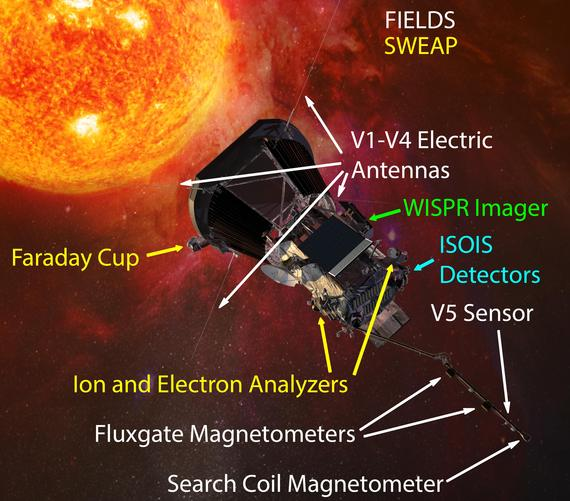
\includegraphics[width=0.9\linewidth,trim=0cm 0cm 0cm 0cm, clip=false]{./Mainmatter/Part_1/images/PSP_All_Instruments}
\cprotect\caption{Localisation des instruments de mesure sur \cacro{PSP}. Les instruments de l'expérience \cacro{FIELDS} sont notés en blanc, et ceux de \cacro{SWEAP} en jaune. Les données utilisées ici proviennent des magnétomètres à saturation (Fluxgate Magnetometers, \cacro{MAGs}) situés sur le bras et de la coupe de Faraday (Faraday Cup, \cacro{SPC}) située juste à côté du bouclier et orientée vers le Soleil. Crédits : la page web de \cacro{FIELDS} (\verb|fields.ssl.berkeley.edu|) et Johns Hopkins University Applied Physics Laboratory.}
\label{fig:sonde_PSP}
\end{figure}
 
 \cacro{FIELDS} [\cite{bale_fields_2016}] mesure le champ magnétique grâce à deux magnétomètres à saturation (\og fluxgate \fg{} en anglais), \cacro{MAGs}, mesurant la composante continue (DC) et les fluctuations à basse fréquence (MHD-ionique) du champ,  et un de type fluxmètre (\og search-coil \fg{}), \cacro{SCM}, donnant accès aux hautes fréquences (ionique-électronique). \cacro{SWEAP} [\cite{kasper_solar_2016}] est quant à elle composée d'une coupe de Faraday (\og Faraday Cup \fg{}), \cacro{SPC}, mesurant les flux globaux ionique et électronique, et d'analyseurs électrostatiques d'ions et d'électrons, \cacro{SPAN}, permettant de séparer leur état de charge. Notre étude concernant plutôt les échelles MHD, les données utilisées proviennent des instruments \cacro{MAGs} et \cacro{SPC}. 

Les données publiquement disponibles au moment où cette étude a été menée (fin 2020) provenaient des quatre premières orbites (\figref{fig:orbit_PSP}). 
\begin{figure}[!ht]
 \centering
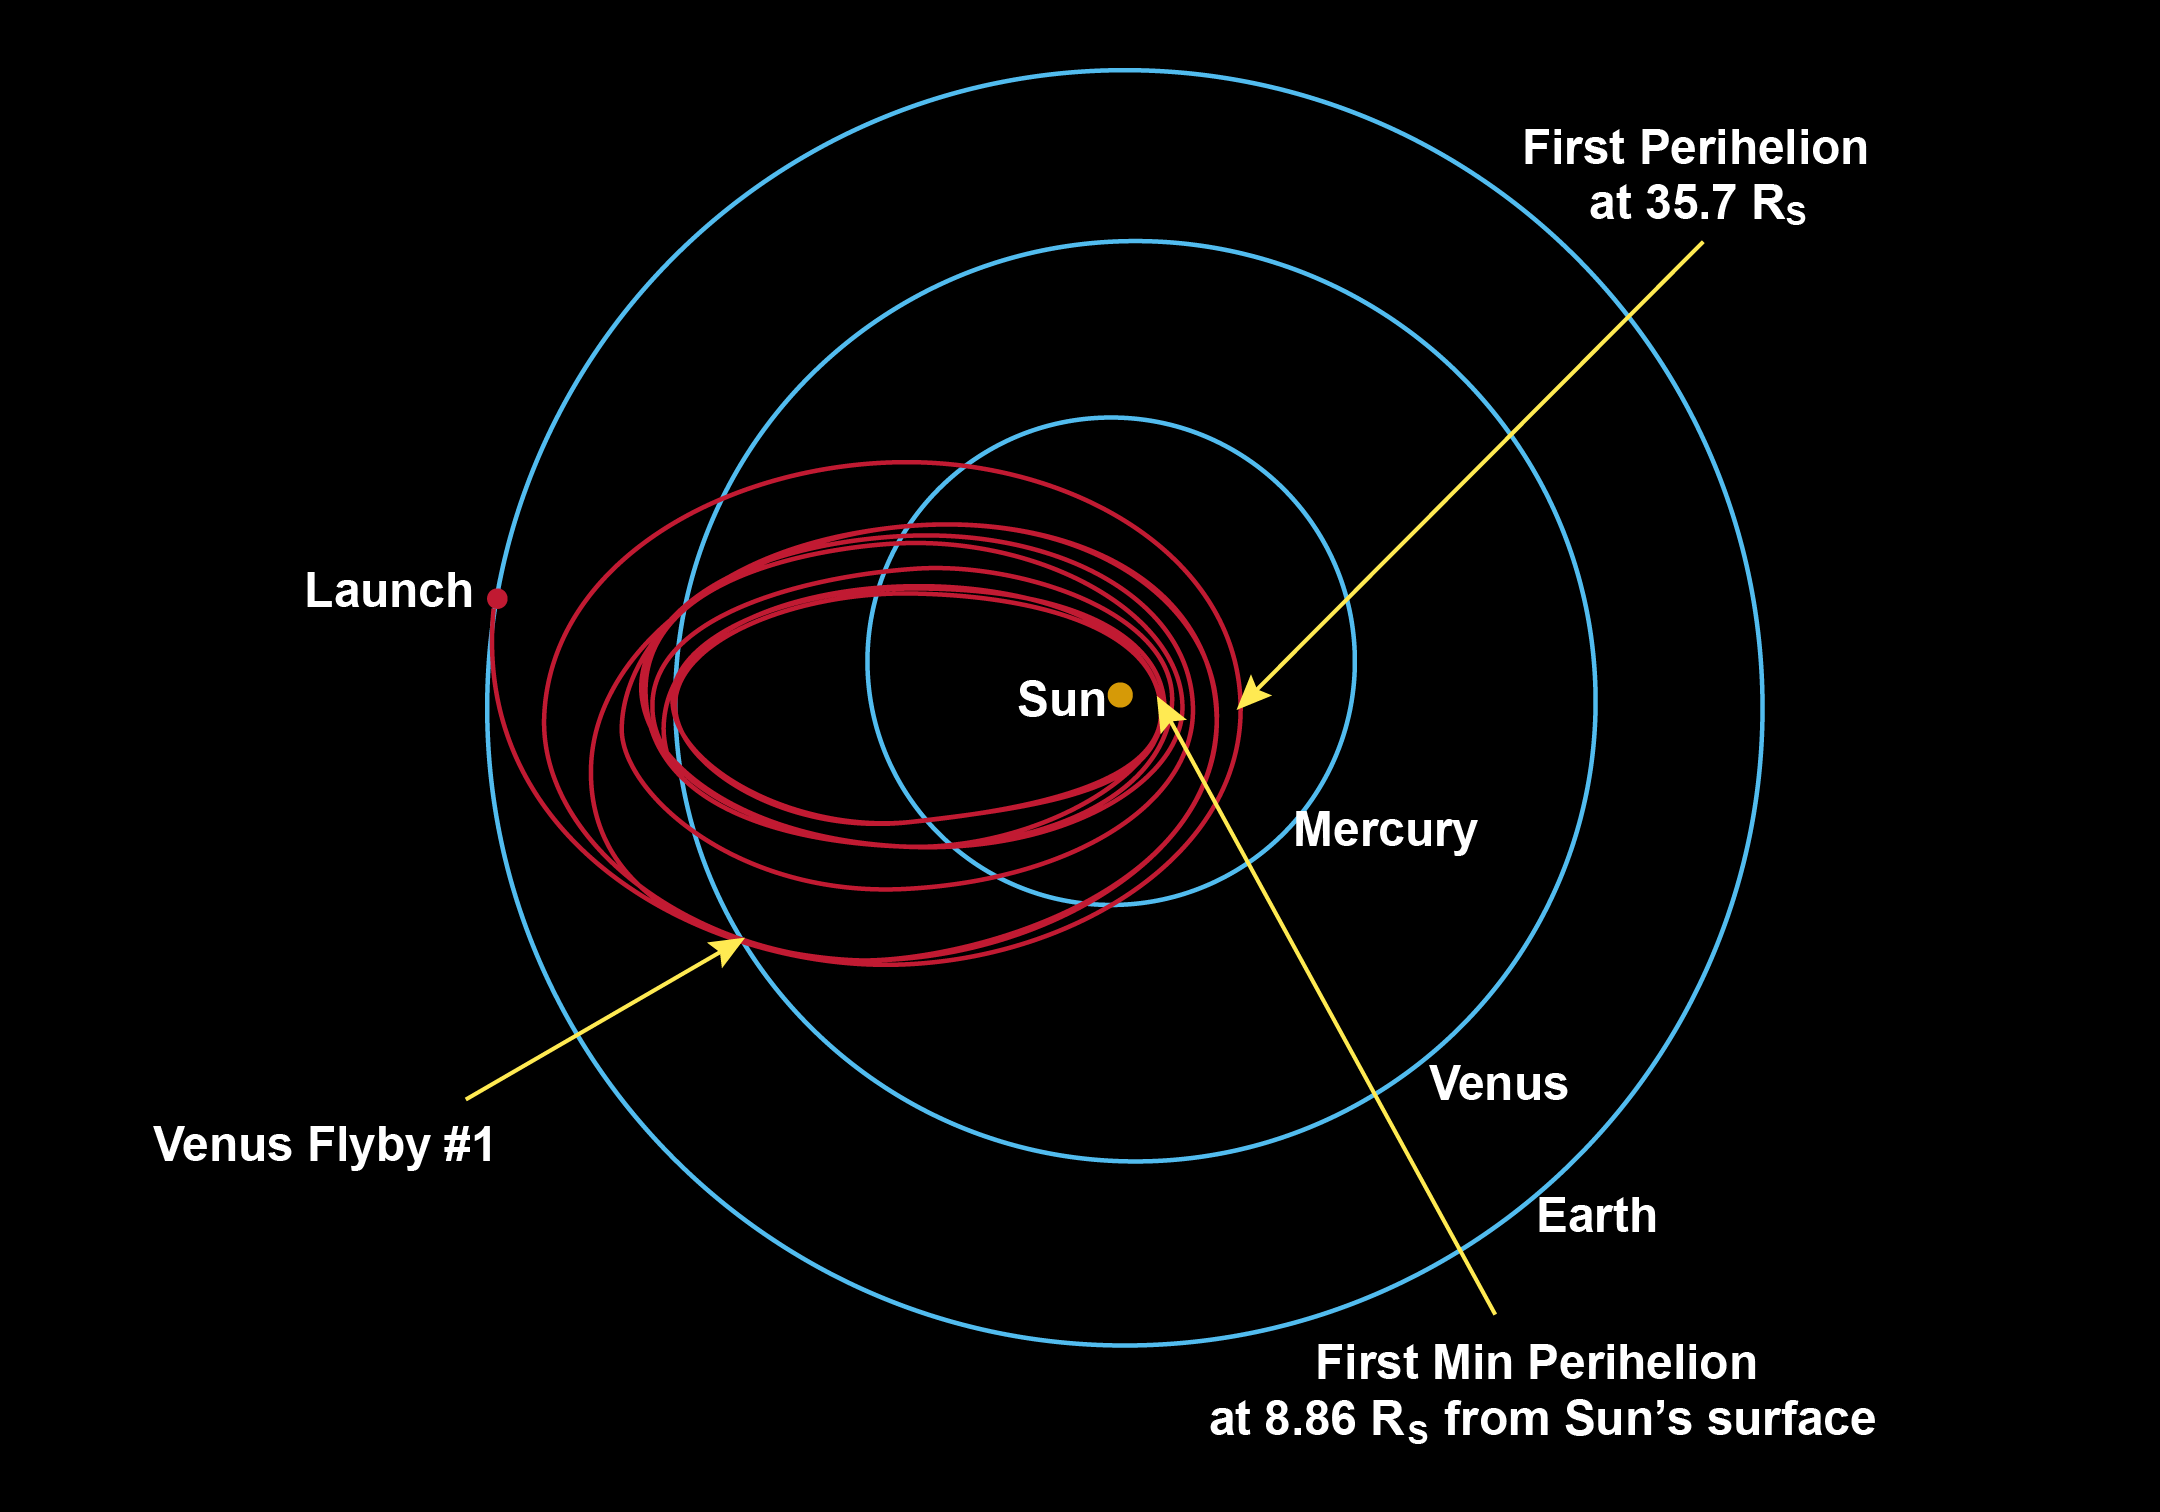
\includegraphics[width=0.9\linewidth,trim=0cm 0cm 0cm 0cm, clip=false]{./Mainmatter/Part_1/images/16-00815_MissionDesign}
\cprotect\caption{Orbites de \cacro{PSP} depuis la date de lancement, le 12 août 2018 à 7h31 \cacro{UTC}. Le premier périhélie à $\SI{35.7}{Rs}$ a été atteint le 6 novembre 2018 à 03h27 \cacro{UTC}. Crédits : la page web de \cacro{PSP} (\verb|http://parkersolarprobe.jhuapl.edu|) et Johns Hopkins University Applied Physics Laboratory.}
\label{fig:orbit_PSP}
\end{figure}
Nous avons choisi d'analyser les données relevées lorsque \cacro{PSP} était proche de son premier périhélie atteint le 6 novembre 2018 à 03h27 \cacro{UTC} vers $\SI{35.7}{Rs}$. Autour de cette position, les données sont relevées dans le vent solaire près du Soleil. Mais peu de lots de données comprenant conjointement les relevés provenant de \cacro{SPC} et ceux provenant de \cacro{MAGs} étaient assez complets pour être traités. Finalement, le jeu choisi a été relevé le 4 novembre entre 00h00 et 02h30. Les données provenant de \cacro{MAGs} y sont résolues à une cadence d'environ $\SI{7}{ms}$ sans temps manquant tandis que celles provenant de \cacro{SPC} sont résolues à $\SI{0,873}{s}$ et montrent $0.15\%$ de temps manquants situés entre 01h08 et 01h13. Ces trous seront comblés par interpolation linéaire et, afin d'avoir la même cadence, les données \cacro{MAGs} sont rééchantillonnées sur la cadence de \cacro{SPC}. Les données analysées sont montrées sur la \figref{fig:data_PSP}.  
 \begin{figure}[!ht]
 \centering
 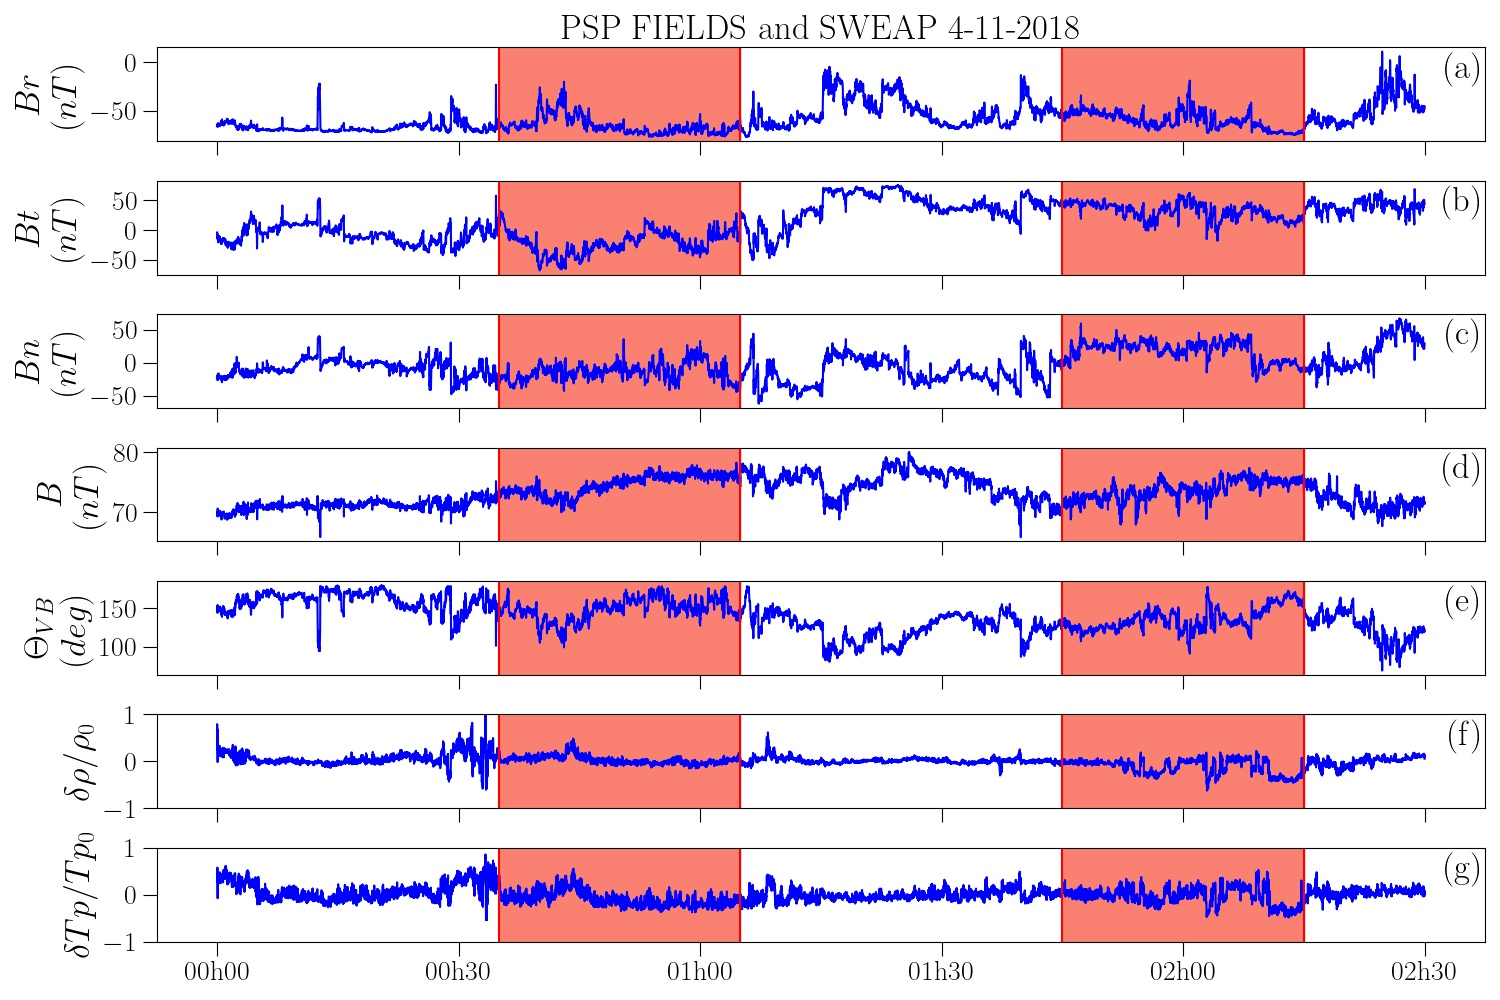
\includegraphics[width=\linewidth,trim=0cm 0cm 0cm 0cm, clip=false]{./Mainmatter/Part_1/images/Fig_04112018H_00_panel}
 \cprotect\caption{Données \cacro{PSP} mesurées dans l'héliosphère interne le 4 novembre 2018. (a) à (c) : les trois composantes du champ magnétique dans le système de représentation \cacro{RTN}. (d) : Norme du champ magnétique. (e) : angle entre le champ de vitesse du fluide et le champ magnétique. (f) et (g) : fluctuations de densité et température relative des protons. Les zones rouges représentent les sous-intervalles utilisés pour le calcul des taux de cascade.}
 \label{fig:data_PSP}
 \end{figure}

Les sous-intervalles choisis pour le calcul des taux de cascade sont marqués en rouge et sont associés à deux niveaux de compressibilité différents. La compressibilité noté $c$ est calculée en prenant l'écart-type, $\text{std}$, des fluctuations de densité, c'est-à-dire $c = \text{std}(\frac{\rho - \rho_0}{\rho_0}) = \text{std}(\frac{\delta \rho}{\rho_0})$. Le premier sous-intervalle, de 00h35 à 01h05 a une compressibilité très faible, $c \sim 8\%$, tandis que le second, de 01h45 à 02h15, est plus compressible, $c \sim 20\%$. Grâce à ces deux intervalles, nous pouvons étudier l'impact des différents niveaux de fluctuations de densité sur le taux de cascade calculé avec la loi isentrope-polytrope et la loi incompressible.

Ces choix de sous-intervalles ont été effectués en considérant un certain nombre d'hypothèses permettant de calculer un taux de cascade tout en réduisant l'incertitude du résultat. Les séries étant temporelles, on utilise l'hypothèse de Taylor\footnote{La validité de l'hypothèse de Taylor dans le vent solaire et en particulier le long de la trajectoire de \cacro{PSP} peut être remise en question [\cite{treumann_applicability_2019,chhiber_contextual_2019}] mais l'obtention d'une hypothèse de remplacement est encore une question ouverte [\cite{parashar_observations_2022}].} [\cite{taylor_spectrum_1937}] qui présuppose que les variations temporelles relevées par la sonde peuvent être interprétées comme des variations spatiales convectées par le flot de plasma à la vitesse moyenne $\boldsymbol{v_0}$. Ainsi, on peut estimer l'incrément spatial $\boldsymbol{\ell}$ à partir de l'incrément temporel $\tau $ via $ \boldsymbol{\ell} \sim \boldsymbol{v_0} \tau$. L'utilisation de l'hypothèse de Taylor donne donc accès aux échelles spatiales dans la direction moyenne du flot. Or le couplage entre le champ magnétique et le fluide implique une forte anisotropie entre les directions parallèle et perpendiculaires au champ magnétique. Par conséquent, si l'angle entre la vitesse et le champ magnétique, $\theta_{VB}$, varie trop fortement, d'importantes variations pourront apparaître dans les résultats du taux de cascade, comme l'ont observé [\cite{hadid_energy_2017}]. Les intervalles ont donc été choisis tel que $\theta_{VB}$ soit relativement stationnaire (ligne (e) de la \figref{fig:data_PSP}). On a aussi considéré des séries temporelles relativement stationnaires pour les autres quantités afin d'assurer une certaine stationnarité/homogénéité statistique. 

L'estimation des moyennes dans le calcul du taux de cascade demande une statistique suffisante, c'est-à-dire des intervalles de durée supérieure à plusieurs fois le temps de corrélation des fluctuations turbulentes [\cite{coburn_third-moment_2015}]. 
[\cite{parashar_measures_2020}] ont estimé le temps de corrélation des données relevées par \cacro{PSP} entre le 3 et le 10 novembre avec des intervalles glissants de 4h, 8h et 24h. En se fiant à cette estimation, le temps de corrélation pour les données utilisées ici (le 4 novembre entre 00h00 et 02h30) est autour de $\SI{500}{s}$, c'est-à-dire un peu moins du tiers de la longueur de nos sous-intervalles ($\SI{30}{min}$). On supposera donc que leur durée convient au calcul d'un taux de cascade. 

\begin{figure}[!ht]
 \centering
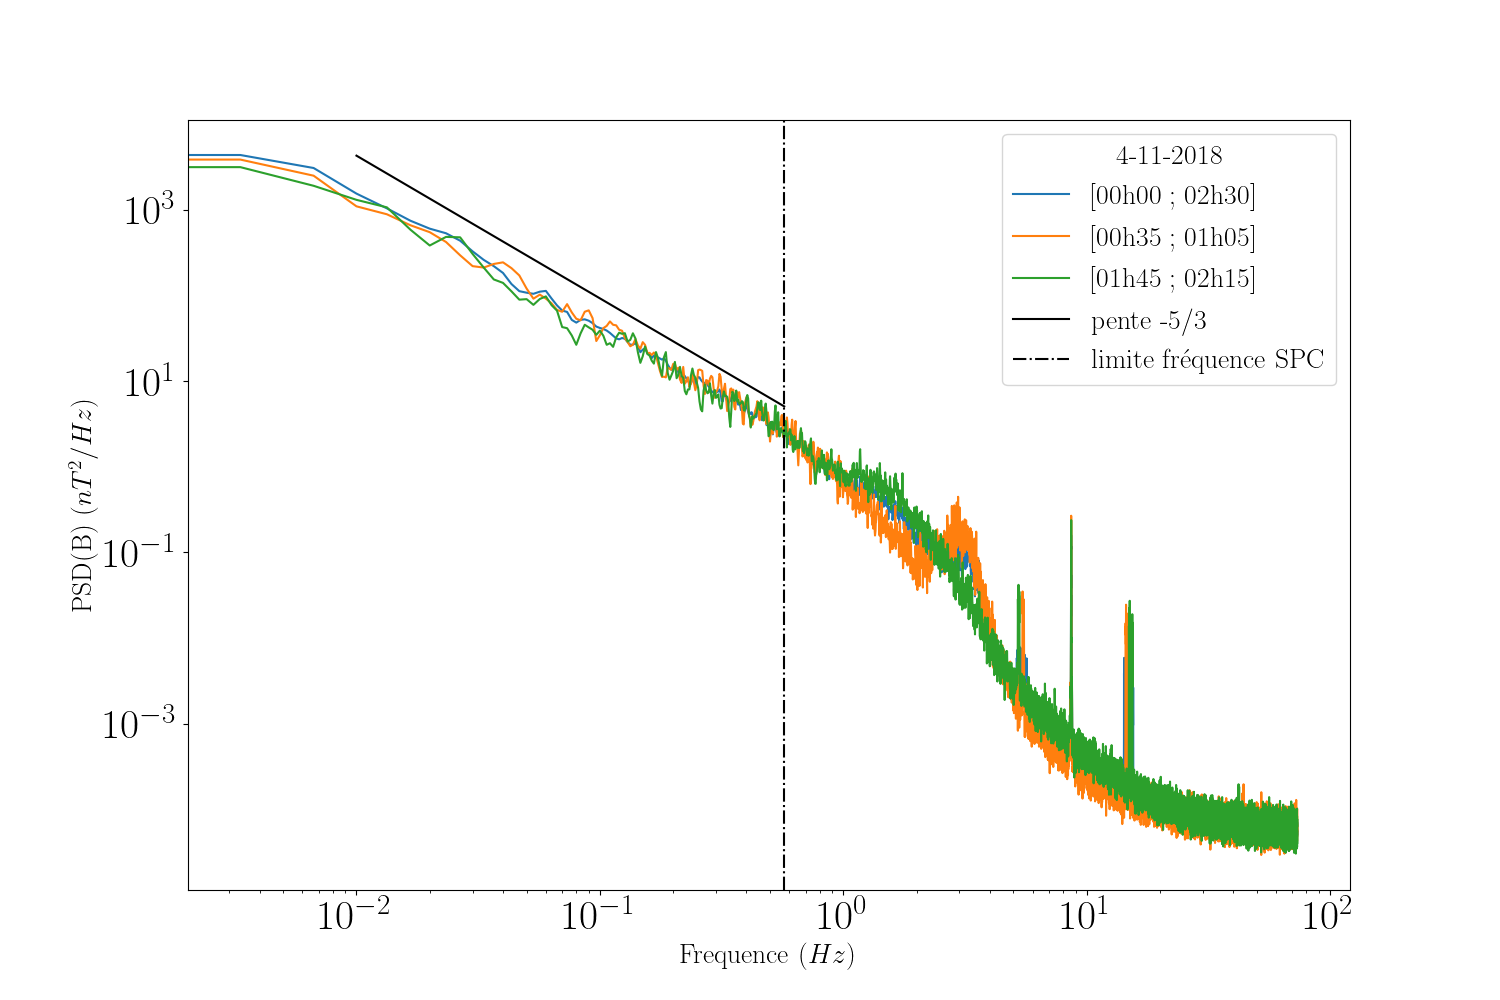
\includegraphics[width=\linewidth,trim=0cm 0cm 0cm 0cm, clip=false]{./Mainmatter/Part_1/images/Fourier2}
\cprotect\caption{Spectre des fluctuations magnétiques pour l'intervalle complet de données (bleu), et les sous-intervalles (orange et vert) obtenue avec les données \cacro{MAGs} non rééchantillonnées à la cadence de \cacro{SPC}. La ligne noire continue indique la pente attendue dans la zone MHD (spectre de type Kolmogorov en $-5/3$) et l'axe vertical la fréquence maximale accessible avec la cadence de \cacro{SPC}.}
\label{fig:spec_PSP}
\end{figure}

Sur la \figref{fig:spec_PSP}, sont tracés les spectres des fluctuations magnétiques obtenus avec les données \cacro{MAGs} non rééchantillonnées de l'intervalle complet et des deux sous-intervalles. Les fréquences qui nous intéressent sont les fréquences inférieures à la cadence de \cacro{SPC}. Pour ces fréquences, la pente des spectres est proche de $-5/3$ (attendue dans la zone \cacro{MHD}). La loi exacte du modèle \cacro{MHD} dérivée dans le Chapitre \ref{ch-13} y semble donc applicable. 
 
 \section{Comparaison des lois incompressible et compressible-isentrope-polytrope avec \ensuremath{\gamma = 1} (isotherme) et \ensuremath{\gamma = 5/3} (adiabatique)}
 \label{sec-142}

Pour ce qui est de la forme de la loi exacte, l'utilisation d'une seule sonde impose deux autres hypothèses. La première correspond à la négligence des termes sources. En effte, ces derniers ne peuvent pas être calculés à cause de leur dépendance en des dérivées locales ($\nabla$ et $\nabla'$) qui ne peuvent être estimées qu'avec des missions multi-sondes telles que \cacro{MMS} ou \cacro{CLUSTER} en orbite autour de la Terre [\cite{andres_energy_2019}]. Physiquement, une telle hypothèse pourrait avoir un impact significatif. Mais d'après l'étude numérique de [\cite{andres_energy_2019}] en turbulence MHD subsonique sur une loi exacte isentrope-isotherme formulée similairement à \eqref{eq:turb_elg_f1} (formulation qui sera considérée ici), les termes flux donnés ci-dessous \eqref{eq:obs_F1} sont dominants tandis que les autres termes sont négligeables ou se compensent. La deuxième hypothèse est celle d'isotropie des fluctuations qui permet d'intégrer tridimensionnellement la loi exacte dans une boule de rayon $\ell = |\boldsymbol{\ell}|$. Cette hypothèse simplificatrice est largement utilisée [\cite{parashar_observations_2022}] mais sa validité peut être remise en cause par l'anisotropie du plasma due au champ magnétique\footnote{Un taux de cascade incompressible intégré axisymétriquement a été investigué par \cite{andres_incompressible_2022} mais une extension compressible reste à faire.}. L'expression du taux de cascade calculée ici est alors : 
\begin{equation}
\label{eq:obs}\varepsilon = F_1 + F_2,
\end{equation}
avec
\begin{eqnarray}
\label{eq:obs_F1} F_1 &=& -\frac{3}{4|\boldsymbol{v_0}|\tau}\left<(\delta (\rho\boldsymbol{v}) \cdot \delta \boldsymbol{v}+ \delta (\rho\boldsymbol{v_A}) \cdot \delta \boldsymbol{v_A}) \delta \boldsymbol{v}  -(\delta (\rho\boldsymbol{v_A}) \cdot \delta \boldsymbol{v}  + \delta (\rho\boldsymbol{v}) \cdot \delta \boldsymbol{v_A}  ) \delta \boldsymbol{v_A} \right> \nonumber, \\ &&\\
\label{eq:obs_F2} F_2 &=& -\frac{3}{4|\boldsymbol{v_0}|\tau}\left<2 \delta \rho  \delta u  \delta \boldsymbol{v}\right>.
\end{eqnarray}
$F_1$ est la contribution dite Yaglom compressible, ne s'annulant pas dans la limite incompressible, tandis que $F_2$ est la contribution d'énergie interne, dépendant des fermetures compressibles. $\rho$ et $u$ y sont calculés pour des cas particuliers de la fermeture isentrope-polytrope définies dans la \tabref{tab:fermetures} :
\begin{itemize}
    \item incompressible (IMHD) : $\rho = \rho_0$, pas de $u$ nécessaire (cette fermeture permet de retrouver la loi \cacro{PP98}),
    \item isentrope-isotherme (CMHDi): $u = c_s^2 \ln(\frac{\rho}{\rho_0})$ obtenu avec la fermeture isentrope-polytrope et $\gamma = 1$,
    \item isentrope-adiabatique (CMHDp) : $u = \frac{c_s^2 -c_{s0}^2}{\gamma(\gamma -1)}$ obtenu avec la fermeture isentrope-polytrope et $\gamma = 5/3$.
\end{itemize}
La vitesse du son $c_s$ est obtenue grâce à la relation des gaz parfaits $c_s^2 = \gamma k_B T_p /m_p$, avec $k_B$ la constante de Boltzmann, $m_p$ la masse des protons, et $T_p$ la température locale des protons. $c_{s0}$ provient de la relation des gaz parfaits calculée avec la température moyenne des protons.
\begin{figure}[!ht]
 \centering
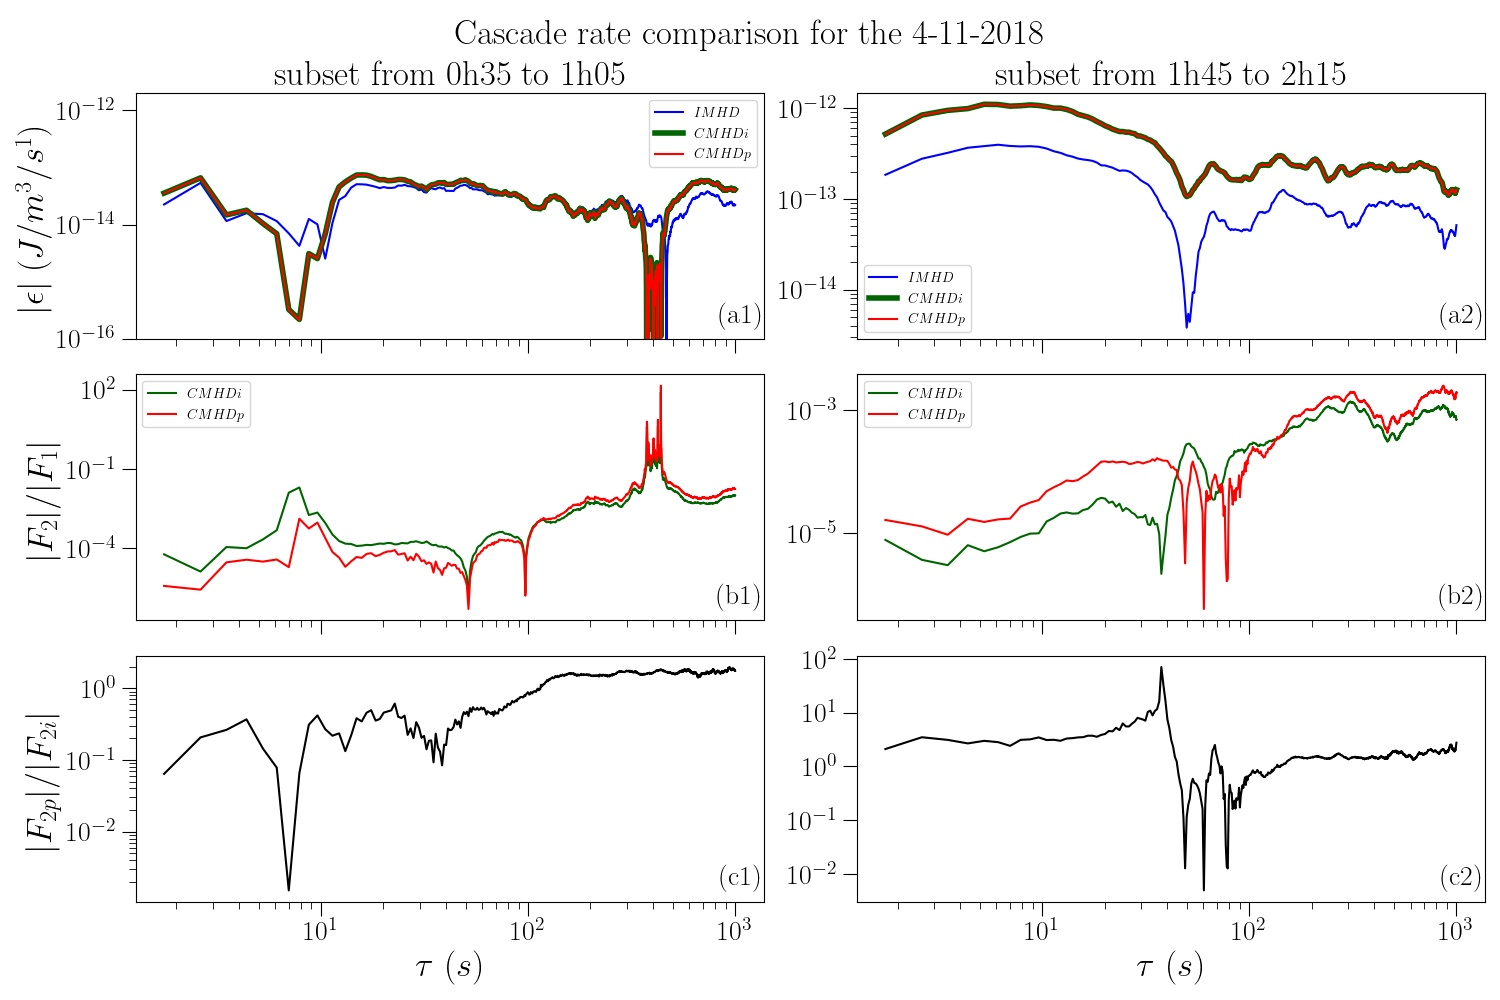
\includegraphics[width=\linewidth,trim=0cm 0cm 0cm 0cm, clip=false]{./Mainmatter/Part_1/images/Fig_04112018H_00_results}
\caption{Comparaison des taux de cascade obtenus avec l'expression de la loi exacte \eqref{eq:obs} et les différentes fermetures pour les sous-intervalles $\{$00h35–01h05$\}$ (à gauche) et $\{$01h45–02h15$\}$ (à droite). (a1)–(a2) : valeur absolue des taux de cascade obtenus avec les fermetures incompressible (IMHD) en bleu, compressibles isentrope-isotherme (CMHDi) en vert et adiabatique (CMHDp) en rouge. (b1)–(b2) : ratio entre la contribution d'énergie interne $F_2$ \eqref{eq:obs_F2} et celle Yaglom compressible $F_1$ \eqref{eq:obs_F1} dans le cas isotherme (vert) et le cas adiabatique (rouge). (c1)–(c2) : ratio entre les contributions de l'énergie interne adiabatique $F_{2p}$ et isotherme $F_{2i}$.}
\label{fig:loi_PSP}
\end{figure}

Sur la \figref{fig:loi_PSP} apparaissent les résultats pour les deux sous-intervalles, le quasi-incompressible à gauche (1) et le plus compressible à droite (2). La première ligne ((a1) et (a2)) montre l'estimation du taux de cascade avec la fermeture IMHD en bleu, la loi CMHDi en vert et CMHDp en rouge. Sur la deuxième ligne ((b1) et (b2)), la contribution d'énergie interne $F_2$ est comparée à la contribution $F_1$ dans les cas isotherme (vert) et adiabatique (rouge). L'impact de la fermeture thermodynamique n'étant portée que par $F_2$, le ratio entre les $F_2$ adiabatique ($F_{2p}$) et isotherme ($F_{2i}$) est donné sur la troisième ligne ((c1) et (c2)).

N'est représentée que la valeur absolue des différentes quantités puisque leur signe nécessite des intervalles plus longs pour statistiquement converger [\cite{coburn_third-moment_2015}, \cite{hadid_energy_2017}]. La question de l'inversion de la cascade potentiellement visualisée à travers le signe du taux ne peut donc pas être étudiée ici. Un taux $\varepsilon$ en valeur absolue quasi-constant peut par contre témoigner d'une convergence. On va donc utiliser la quasi-constance de $\varepsilon$ pour définir une zone inertielle. Pour le premier intervalle, sur le graphique (a1) de la \figref{fig:loi_PSP}, les $\varepsilon$ montrent des variations avant $\tau \sim \SI{10}{s}$ et après  $\tau \sim \SI{400}{s}$ et restent quasiment constant au centre. On supposera donc que cette zone centrale correspond à une zone inertielle. À grande échelle, ces variations proviennent de $F_1$ et se reflètent dans la brusque augmentation apparaissant sur le graphique (b1) de la \figref{fig:loi_PSP}. Ils s'avère que ces variations sont accompagnées de changements de signe. Pour le second intervalle, sur le graphique (a2) de la \figref{fig:loi_PSP}, le signe ne varie pas, il reste positif contrairement à ce que pourrait laisser présager le creux apparaissant en $\tau \sim \SI{50}{s}$. En se fiant à la quasi-constance du niveau de $\varepsilon$, nous limitons l'interprétation d'une zone inertielle à l'intervalle $\tau \in [50;800]\SI{}{s}$. 

 Le graphique (a2) de la \figref{fig:loi_PSP} met en avant le rôle de la compression dans le taux de cascade : les taux de cascade compressibles sont plus élevés d'un facteur 2 à 3 par rapport au taux incompressible, alors que le graphique (a1) de la \figref{fig:loi_PSP} provenant de données bien moins compressible montre des niveaux similaires. Cette observation coïncide avec de précédentes, issues de données du vent solaire [\cite{banerjee_scaling_2016}, \cite{hadid_energy_2017}, \cite{andres_evolution_2021}]. Par contre, les deux modèles compressibles montrent les mêmes résultats. La raison de cette convergence est révélée par les graphiques (b1) et (b2) de la \figref{fig:loi_PSP} : la contribution de $F_2$ est bien négligeable devant celle de $F_1$. Le facteur 3 observé précédemment provient donc de la prise en compte de la densité dans $F_1$.  Même si l'impact du terme dépendant de la fermeture à une importance moindre dans le taux total, nous pouvons en examiner l'effet sur les graphiques (c1) et (c2) de la \figref{fig:loi_PSP}. Aux grandes échelles ($\tau > \SI{100}{s}$), les deux fermetures apportent une contribution similaire tandis qu'à plus petite échelle (hors de la suspectée zone inertielle pour le deuxième intervalle), un ordre de grandeur de différence apparaît. Dans le cas du premier intervalle, la fermeture isotherme contribue plus que l'adiabatique tandis que dans le cas du deuxième intervalle, c'est le contraire. Une interprétation complète de cette différence de comportement ne peut être apportée avec cette étude de cas et nécessite une analyse statistique. Cette analyse, effectuée ultérieurement par \cite{brodiano_statistical_2022} dans les données \cacro{PSP} montre que $\left<F_2\right>$ (en notant $\left<\right>$ la moyenne sur les échelles et en adoptant nos notations des contributions aux taux de cascade) apparaît statistiquement un à deux ordres de grandeur en dessous de $\left<F_1\right>$, et que le facteur $\num{3}$ entre les taux compressibles et le taux incompressible n'est pas retrouvé sauf pour des cas particuliers. Les cas que nous avons étudiés semblent donc dans la norme pour le premier point vérifié, mais, pour le dernier point, notre deuxième sous-intervalle entre dans la classe des cas particuliers. Ils montrent aussi que plus la compressibilité est forte, plus $\left<F_2\right>$ peut venir concurrencer $\left<F_1\right>$ voire, pour certains cas, le surpasser. Près du Soleil, ils notent aussi que $\left<F_{2p}\right>$ est supérieur à $\left<F_{2i}\right>$ en moyenne.

Cette étude de cas préliminaire, publiée dans \cite{simon_general_2021} et validée statistiquement par \cite{brodiano_statistical_2022}, a donc permis de visualiser l'impact de la compression sur l'estimation du taux de cascade et l'apport potentiel d'une fermeture par rapport à une autre dans des données réelles du vent solaire. 

\section{Application statistique préliminaire dans des données localisées dans la magnétogaine terrestre}
\label{sec-143}

Le plasma dans la magnétogaine est plus compressible que dans le vent solaire [\cite{hadid_compressible_2018}] et d'après \cite{livadiotis_long-term_2018}, $1<\gamma<5/3$. Il est aussi exploré par de multiples missions, en particulier des missions multi-sondes comme \cacro{MMS} qui comprend quatre satellites en orbite autour de la Terre depuis 2015 (\figref{fig:MMS}). 
\begin{figure}[!ht]
 \centering
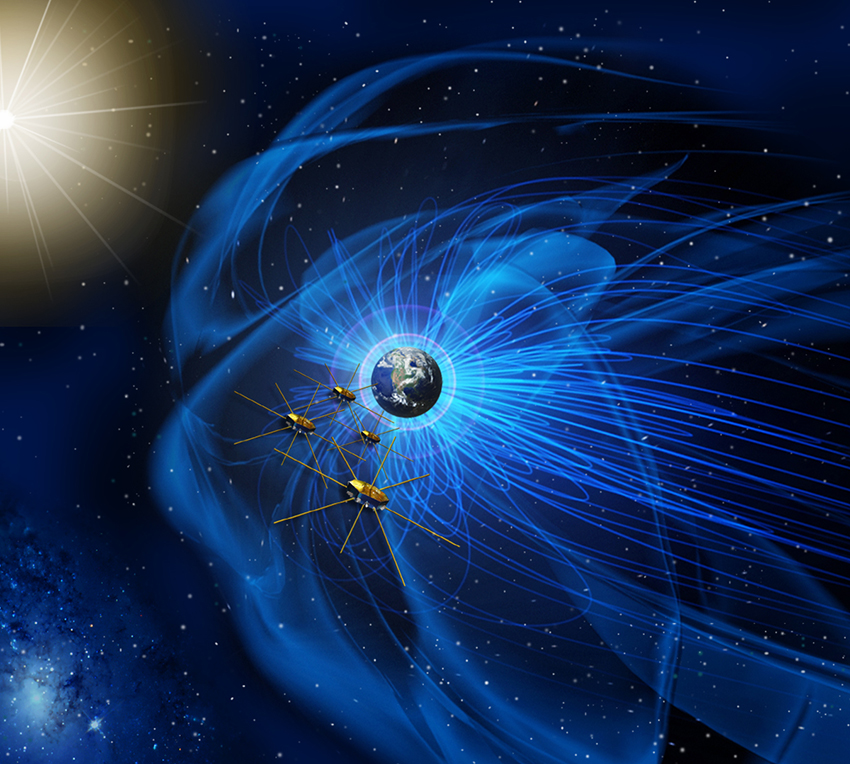
\includegraphics[width=0.7\linewidth,trim=0cm 6cm 6cm 4cm, clip=true]{./Mainmatter/Part_1/images/MMS_mission}
\cprotect\caption{Vue d'artiste de la mission \cacro{MMS}. Crédits : la page web de \cacro{MMS}/\cacro{NASA} (\verb|https://www.nasa.gov/mission_pages/mms|).}
\label{fig:MMS}
\end{figure}

À partir d'une douzaine de cas parmi ceux utilisés par \cite{andres_energy_2019}, nous avons vérifié si l'on retrouve, dans la magnétogaine, les résultats de notre étude de cas effectuée avec les données de \cacro{PSP}. Les données utilisées ont été relevées par les instruments \cacro{FPI} pour ce qui est des moments de la fonction de distribution des particules, et \cacro{FGM}, pour le champ magnétique, pendant 12 intervalles de temps entre 2015 et 2017. L'étude, similaire à celle effectuée avec les données de \cacro{PSP}, est menée séparément sur les quatre satellites de la constellation (48 résultats). 

Concernant les quantités estimées, les notations sont les mêmes que celles utilisées dans la section \ref{sec-133}. La \figref{fig:loi_MMS} montre l'emplacement des 48 résultats pour lesquels les fluctuations de densité (compressibilité $c$) varie de $20\%$ à $60\%$ (visualisé via l'échelle de couleur) dans deux diagrammes ayant pour abscisse le rapport entre les taux moyen compressible $\left<\varepsilon_{CMHDp}\right>$ obtenu avec $\gamma = 5/3$ (loi adiabatique, CMHDp) et incompressible $\left<\varepsilon_{IMHD}\right>$. Le diagramme de gauche a pour ordonnée le rapport entre les contributions d'énergie interne $\left<F_{2p}\right>$ et Yaglom compressible $\left<F_{1}\right>$ de la loi adiabatique et celui de droite le rapport entre les contributions d'énergie interne adiabatique et isentrope-isotherme, respectivement $\left< F_{2p} \right>$ et $\left< F_{2i} \right>$. 
\begin{figure}[!ht]
 \centering
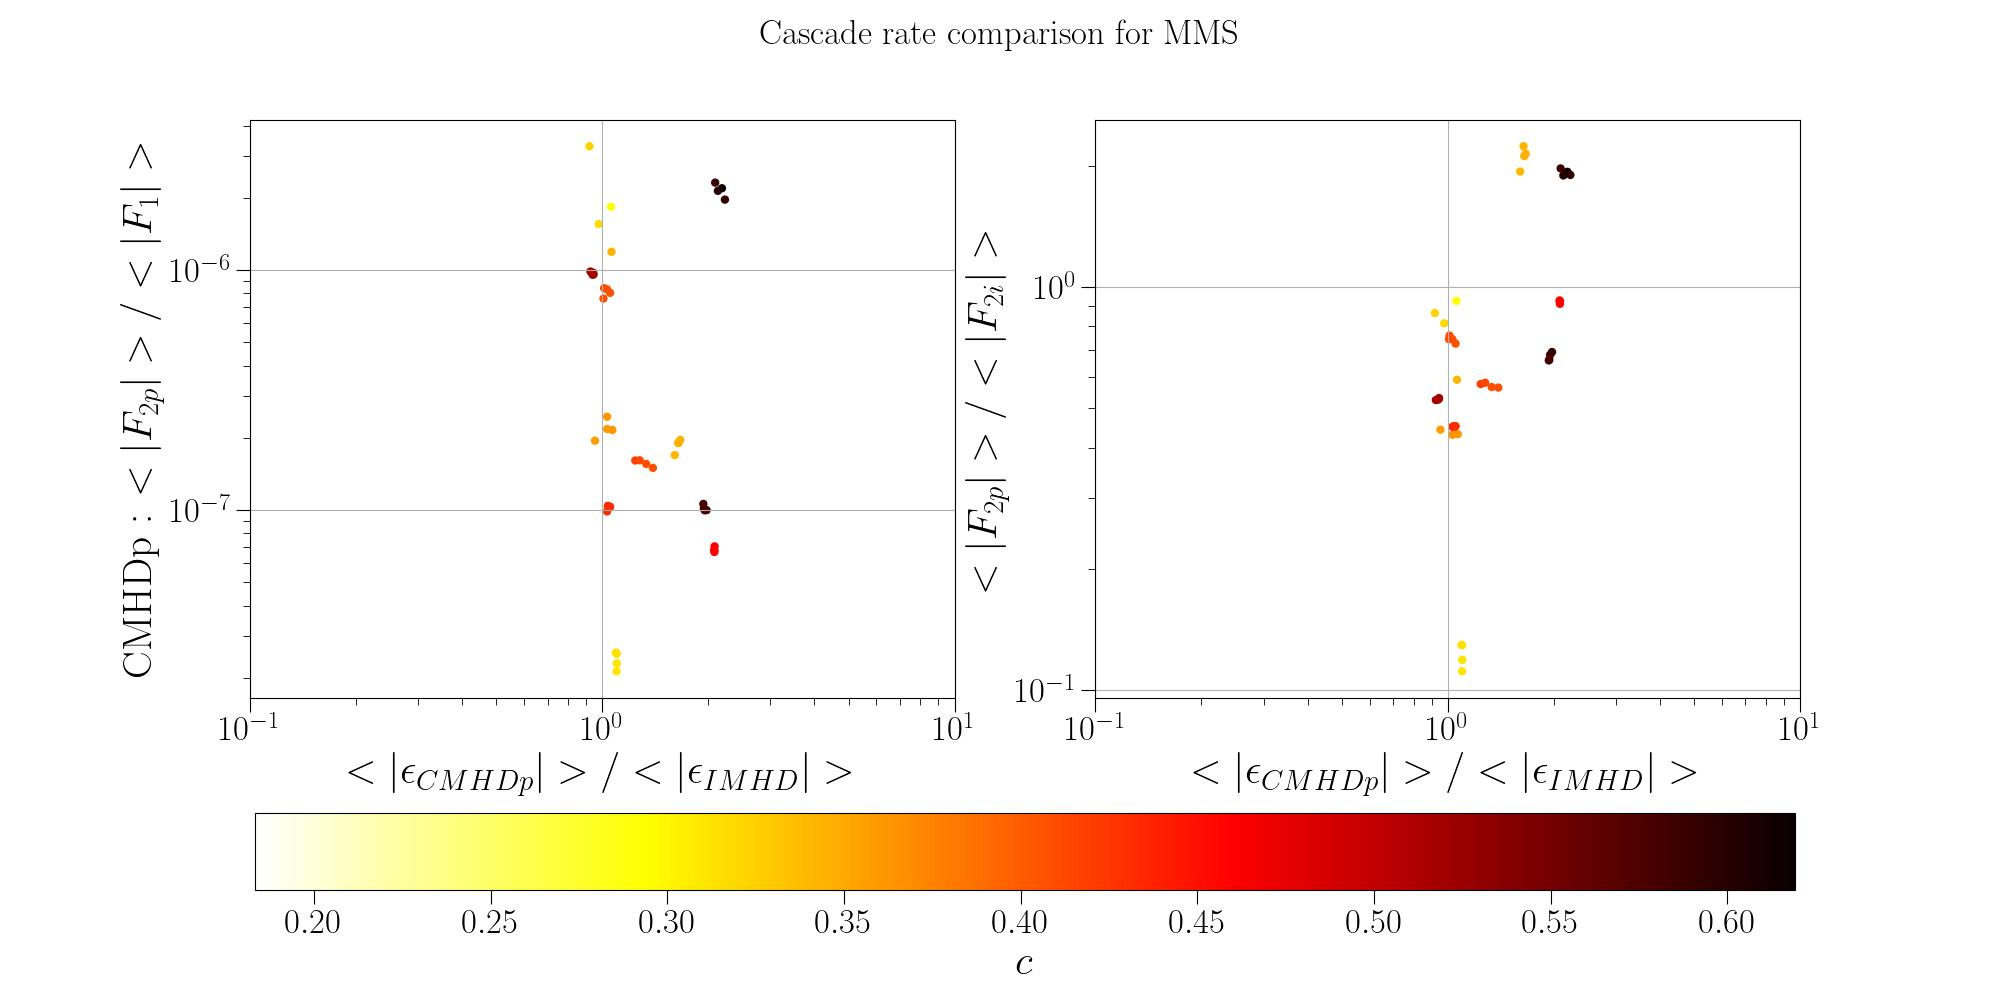
\includegraphics[width=\linewidth,trim=3cm 0cm 3cm 3cm, clip=true]{./Mainmatter/Part_1/images/cascade_comp_MMS_2}
\cprotect\caption{Résumé de l'étude statistique préliminaire menée sur 12 intervalles des quatre satellites de \cacro{MMS}. Couleurs : compressibilité $c $ de l'intervalle. Abscisses : rapport entre le taux de cascade compressible adiabatique (CMHDp, $\gamma = 5/3$) et incompressible (IMHD). À gauche : pour CMHDp, rapport entre les contributions d'énergie interne $F_2$ et Yaglom compressible $F_1$. À droite : rapport entre les contributions d'énergie interne adiabatique $F_{2p}$, et isotherme $F_{2i}$ ($\gamma = 1$).}%
\label{fig:loi_MMS}
\end{figure}

Cette étude révèle de plus importantes fluctuations de densité dans la magnétogaine que celles relevées pour les données de \cacro{PSP}. Dans les cas les plus compressibles, le taux de cascade compressible semble pouvoir doubler par rapport au taux incompressible (points rouges éloignés de la verticale centrale). Cependant, la contribution d'énergie interne moyenne y est encore plus négligeable que dans les données de \cacro{PSP}, 5 à 8 ordres de grandeurs plus faibles que la contribution Yaglom compressible moyenne comme le montre le diagramme de gauche. Sur le diagramme de droite, on voit que $\left<F_{2p}\right>$ à tendance à être un peu plus faible que $\left<F_{2i}\right>$ mais qu'il peut aussi être environ deux fois plus important. Cette dernière observation montre un comportement inverse du comportement moyen observé à tout rayon solaire dans le vent solaire par \cite{brodiano_statistical_2022}, mais demanderait plus de statistique pour être confirmée. 
 
 Cette étude dans les données de \cacro{MMS} est restée préliminaire, l'intérêt du travail ayant dévié vers l'effet de l'anisotropie de pression (voir Partie \ref{part_2}). Par la suite, une autre contribution pourrait être étudiée grâce à la constellation de satellites de \cacro{MMS} : celles des termes sources, impossible à analyser avec \cacro{PSP}. La caractéristique multi-sondes de cette mission peut en effet permettre le calcul complet des lois exactes compressibles. Cela a, par exemple, été effectué dans le cadre isotherme par \cite{andres_energy_2019}. Il serait aussi intéressant d'étudier dans les données les contributions au taux de cascade apportées par les différentes formulations ayant été analytiquement dérivées dans le chapitre précédent, en particulier les contributions des termes flux dépendant des pressions magnétique et thermodynamique, ou celle du flux de chaleur.

\newpage
\section{Synthèse de l'étude de cas observationnels issus des données de PSP}
\label{synt-14}
\fcolorbox{blue}{white}{\begin{minipage}[c]{\linewidth}
\paragraph{Données choisies : } instruments \cacro{SPC}/\cacro{SWEAP} et \cacro{MAGs}/\cacro{FIELDS} présents sur la sonde \cacro{PSP}, mesures relevées le 4 Novembre 2018, comparaison d'un intervalle quasi-incompressible et d'un plus compressible. \\

 \paragraph{Hypothèses nécessaires à l'utilisation de données in-situ issues d'une mission composée d'une seule sonde pour l'estimation de taux de cascade : } 
 \begin{itemize}
     \item taille d'intervalle supérieure à plusieurs fois le temps de corrélation des fluctuations turbulentes,
     \item hypothèse de Taylor, $\boldsymbol{\ell} \sim \boldsymbol{v_0} \tau$,
     \item angle $\theta_{VB}$ quasi-stationnaire,
     \item négligence des termes sources dans la loi exacte, valide si vent subsonique et avec la formulation f1 de la loi exacte \cacro{MHD},
     \item intégration isotrope de la loi exacte, validité à nuancer tant que l'angle $\theta_{VB}$ reste quasi-stationnaire.
 \end{itemize}
\end{minipage}}

 \fcolorbox{red}{white}{\begin{minipage}[c]{\linewidth}
 \paragraph{Loi exacte analysée : } $\varepsilon = F_1 + F_2$ avec
 \begin{eqnarray*}
  F_1 &=& -\frac{3}{4|\boldsymbol{v_0}|\tau}\left<(\delta (\rho\boldsymbol{v}) \cdot \delta \boldsymbol{v}+ \delta (\rho\boldsymbol{v_A}) \cdot \delta \boldsymbol{v_A}) \delta \boldsymbol{v}  -(\delta (\rho\boldsymbol{v_A}) \cdot \delta \boldsymbol{v}  + \delta (\rho\boldsymbol{v}) \cdot \delta \boldsymbol{v_A}  ) \delta \boldsymbol{v_A} \right> \\
  F_2 &=& -\frac{3}{4|\boldsymbol{v_0}|\tau}\left<2 \delta \rho  \delta u  \delta \boldsymbol{v}\right>
 \end{eqnarray*}
 \paragraph{Fermetures : }
 \begin{itemize}
     \item incompressible : $\rho = \rho_0$, pas de $u$ nécessaire,
     \item isentrope-isotherme : $u = c_s^2 \ln(\frac{\rho}{\rho_0})$ et $\gamma = 1$,
     \item isentrope-adiabatique : $u = \frac{c_s^2 -c_{s0}^2}{\gamma(\gamma -1)}$ et $\gamma = 5/3$.
 \end{itemize}
 
 \paragraph{Conclusion : }
 \begin{itemize}
     \item apport potentiellement substantiel de la compression via la densité dans les termes de type $F_1$ indépendant de la fermeture,
     \item apport de la fermeture important dans $F_2$ à petite échelle,
     \item $F_2$ négligeable devant $F_1$ pour les fermetures compressibles et dans les cas analysés.
 \end{itemize}
 
 Ces résultats sont publiés dans \cite{simon_general_2021}, statistiquement validés par \cite{brodiano_statistical_2022} et étendus dans la magnétogaine à travers une étude statistique préliminaire effectuée dans les données de \cacro{MMS} (section \ref{sec-133}). 
 \end{minipage}}


\chapitrestar{Conclusion}{CONCLUSION}{ch-15}
\chapter*{Conclusion}
 \addcontentsline{toc}{chapter}{Conclusion}
 \adjustmtc
\renewcommand\partie{\Partie\ CONCLUSION}
\label{ch-15}

	
%\bigskip
%\minitoc  

Depuis 1998 et la loi exacte de {\sc Politano} et {\sc Pouquet} étendant aux plasmas incompressibles, la théorie de Kolmogorov décrivant la cascade turbulente à travers des lois exactes, de multiples extensions ont été proposées prenant en compte la compressibilité. 

Dans cette partie \ref{part_1}, nous nous sommes concentrés sur l'effet de fermetures thermodynamiques dépendant d'une pression isotrope. Un premier chapitre (synthèse section \ref{synt-12}) pose le problème de la compressibilité dans les modèles fluides et analyse différentes possibilités de fermeture basées sur la théorie thermodynamique. La question qui se pose alors est celle de l'impact de la compressibilité sur la turbulence. Ma contribution pour y répondre est développée à travers les chapitres \ref{ch-13} et \ref{ch-14}. 

Dans le Chapitre \ref{ch-13} (synthèse section \ref{synt-13}), un cadre analytique est démontré à travers l'extension de la théorie des lois exactes. La stratégie mise en œuvre ne repose pas sur une fermeture thermodynamique, a contrario de celles entreprises dans la littérature [\cite{galtier_exact_2011,banerjee_exact_2013,banerjee_kolmogorov-like_2014,andres_alternative_2017}], mais plutôt, sur l'équation de densité d'énergie interne. La loi exacte résultante obtient ainsi un caractère général et la fermeture ne devient qu'un <<détail>>, une hypothèse, à ne considérer qu'à la fin du calcul en fonction du besoin. Par ce biais, est abordé l'objectif initial de cette partie du travail : obtenir une loi valable dans la zone inertielle isentrope pour une fermeture polytrope décrivant ainsi la cascade turbulente dans les plasmas de manière plus réaliste et versatile que la fermeture isotherme utilisée jusqu'à présent. La première formulation (f1) proposée pour répondre à cet objectif est inspirée du travail dans le cadre isentrope-isotherme de \cite{andres_energy_2018}. Elle a permis l'étude comparative, dans deux jeux de données issus de la mission \ac{PSP}, de l'impact de la compression et des fermetures isentropes-isotherme ($\gamma = 1$) et isentrope-adiabatique ($\gamma = 5/3$) sur la cascade turbulente. Cette étude fait l'objet du Chapitre \ref{ch-14}  (synthèse section \ref{synt-14}) où elle est étendue dans la magnétogaine à travers l'amorçage d'une étude statistique utilisant les données de MMS. L'intérêt de la formulation f1 est que les termes sources impossibles à calculer à cause des caractéristiques de la mission \ac{PSP} (une seule sonde) ont préalablement été numériquement démontrés comme négligeables dans le taux de cascade total par \cite{andres_energy_2018} dans les cadre isotherme. La deuxième formulation (f2) de la loi exacte a initialement vu le jour comme une conséquence du travail analytique qui sera présenté dans la partie \ref{part_2}, relaxant l'isotropie de pression, mais le résultat, dépendant de $p/\rho$, peut s'avérer plus adapté à l'application d'une fermeture thermodynamique. La troisième et dernière formulation (f3) est la plus récente et s'inspire du travail sur le flux de chaleur dans l'équation d'énergie interne qui s'est révélée nécessaire lors de l'étude numérique qui sera présentée dans la partie \ref{part_3}. Ce résumé des résultats obtenus avec pression isotrope reflète la structure chronologique de l'ensemble du travail effectué et présenté dans ces trois parties, la méthode scientifique mise en œuvre et les points méthodologiques utilisés. 

En termes de physique, cette partie propose un cadre d'étude de l'impact de la compression dans sa forme la plus <<simple>> : une densité variable, une pression isotrope, une énergie interne et un flux de chaleur souvent négligé. Ces grandeurs nous permettent de fermer le modèle fluide par des relations basées sur des hypothèses thermodynamiques telles que l'isentropie, l'isothermie ou la polytropie. À travers l'analyse de ces hypothèses et leur application dans les anciennes descriptions de la cascade turbulente, quatre possibilités majeures de fermeture ont émergé. La première, isentrope-isotherme est la première à avoir été utilisée dans l'extension des lois exactes [\cite{galtier_exact_2011,banerjee_exact_2013,andres_alternative_2017}]. La deuxième, isentrope-polytrope, introduite en HD [\cite{banerjee_kolmogorov-like_2014}], est celle qui nous a permis de généraliser la méthode d'obtention des lois exactes à toutes fermetures en utilisant l'équation d'énergie interne, elle prend en compte l'existence d'un $\gamma$ et reflète un peu mieux la pluralité de transformations thermodynamiques observée dans les plasmas spatiaux et astrophysiques. La troisième, polytropique, basée sur un $\gamma$ et un $\sigma$, lie le flux de chaleur au travail de pression et étend un peu plus loin les possibilités d'application des lois exactes. De la dernière, isotherme, émerge la loi exacte compressible qui semble la plus simple malgré la prise en compte des flux de chaleur. 

Pour ce qui est de l'impact de la compression et des fermetures observé dans l'étude du taux de cascade dans le vent solaire, l'étude de cas comparative montre que la compression peut jouer un rôle important dans la cascade, mais, dans les cas étudiés, la fermeture isentrope-adiabatique ou isentrope-isotherme a peu d'impact malgré le rôle qu'elle joue à travers l'énergie interne. Les termes dominants s'avèrent en effet être ceux n'en dépendant pas. On peut aussi les interpréter comme ceux subsistant dans le cas d'une fermeture isobare. Ce travail pose ainsi les bases d'une étude observationnelle, plus générale, complète et systématique, de l'impact de compression et des fermetures sur la turbulence dans les plasmas spatiaux. Cette étude est laissée au futur car le vent solaire ayant la particularité d'être peu collisionnel et magnétisé, nous nous sommes intéressés à un autre type de fermeture qui a orienté le travail dans une autre direction : celle de l'effet de l'anisotropie de pression.  













\cleardoublepage\phantomsection
\pagepart
	{PARTIE II: Etude analytique de l’effet de l'anisotropie de pression}	
	{part_2}
	{PARTIE II : Chapitre}
	{PARTIE II : }
	{\quotechapt{\personne{Hardy}[Thomas]\footnote{\textsc{Loin de la foule déchainée}, publiée en version originale anglaise en 1874} (1849-1927), artiste, écrivain, poète, romancier.}{
  La collision de tous les sentiments contradictoires qui l'agitaient avait produit la neutralité, et aucun d'eux n'était capable de lui communiquer le mouvement. Citation extraite de la traduction française de \cite{hardy_far_1874}.}}

\chapitrestar{Introduction}{INTRO}{ch-20}
Les fonctions de distribution de vitesse des ions observées dans le vent solaire sont généralement anisotropes le long des directions parallèle et perpendiculaires au champ magnétique [\cite{marsch_pronounced_1981}, \cite{matteini_evolution_2007}, \cite{bale_magnetic_2009}]. Le champ magnétique, interagissant avec les ions, rend le milieu anisotrope et les collisions, trop peu nombreuses, échouent à l'isotropiser. Ce type d'anisotropie a tout d'abord été modélisé par [\cite{chew_boltzmann_1956}] à travers une pression de forme tensorielle et diagonale (gyrotrope) et supposant l'isentropie du modèle. Ce modèle, nommé \cacro{CGL} en hommage aux auteurs, sera présenté plus en détail dans le Chapitre \ref{ch-21} de cette deuxième partie. Il y sera accompagné de l'extension proposée pour la théorie de Kolmogorov, prenant en compte un tenseur de pression. Ensuite dans le Chapitre \ref{ch-22}, nous nous poserons la question suivante : l'incompressibilité est-elle compatible avec la gyrotropie de pression ? Et, dans le Chapitre \ref{ch-23}, nous 
généraliserons la loi pour la \cacro{MHD} au modèle bi-fluide dépendant des ions et des électrons.

Dans cette partie qui concentre le cœur analytique du travail effectué, nous conserverons l'hypothèse d'une zone inertielle isentrope et nous ne regarderons pas en détail l'impact sur la cascade des composantes non gyrotropes du tenseur de pression.


\chapitre{Loi exacte pour le modèle CGL}{ch-21}
Dans le vent solaire, utiliser un modèle \cacro{MHD} compressible avec pression isotrope peut s'avérer ardu à justifier en présence d'un champ magnétique et d'un faible nombre de collisions. Il faut prendre en compte, a minima, une pression gyrotrope par exemple en utilisant le modèle dit \cacro{CGL}. C'est le but de ce chapitre : décrire la cascade turbulente d'énergie totale à travers une loi exacte associée au modèle \cacro{CGL}. Encore une fois, on ne réduira le champ d'application qu'après avoir obtenu une loi plus générale, valable pour tout tenseur de pression. Les nouveaux résultats exposés ici ont fait l'objet principal de l'article [\cite{simon_exact_2022}].

\section{D'un tenseur de pression dans le modèle fluide au modèle CGL}
\label{sec-211}

Dans le cadre général défini à partir de l'équation de Vlasov et menant au modèle \cacro{MHD}, la pression et le flux de chaleur sont définis comme des tenseurs d'ordre 2 et 3 respectivement. La pression, $\overline{\boldsymbol{P}} $, est un tenseur symétrique obtenu en effectuant le produit de deux vecteurs vitesse tandis que le flux de chaleur s'obtient à partir du produit de trois vecteurs vitesse. 

  Dans la Partie \ref{part_1}, la pression était supposée isotrope, c'est à dire $\overline{\boldsymbol{P}} = p \overline{\boldsymbol{I}}$ avec $\overline{\boldsymbol{I}}$ le tenseur identité. Dans le modèle \cacro{CGL}, elle est définie comme gyrotrope par rapport à la direction du champ magnétique, notée $\boldsymbol{b}$. On considère donc deux pressions, une dite parallèle $p_{\parallel}$ et une perpendiculaire $p_{\perp}$. Dans un repère cartésien orienté tel que $\boldsymbol{b}$ coïncide avec la direction $\boldsymbol{e_z}$, le tenseur s'écrit : 
\begin{equation*}
 \overline{\boldsymbol{P}} = \left( \begin{array}{ccc}
                                    p_{\perp} & 0 & 0 \\
                                    0 & p_{\perp} & 0 \\
                                    0 & 0 & p_{\parallel} 
                                    \end{array} \right).   
\end{equation*}
Plus généralement, on peut l'écrire $ \overline{\boldsymbol{P}} = p_{\perp} \overline{\boldsymbol{I}} + \left(p_{\parallel} - p_{\perp}\right) \boldsymbol{b}\boldsymbol{b} $. La partie isotrope de la pression, $p = \frac{1}{3} \overline{\boldsymbol{P}} : \overline{\boldsymbol{I}} = \frac{1}{3} \left(2 p_{\perp} + p_{\parallel} \right) $, est obtenue en faisant le produit dual "$:$" entre $\overline{\boldsymbol{P}}$ et  $\overline{\boldsymbol{I}}$, ce qui revient à considérer la trace de $\overline{\boldsymbol{P}}$. Cela permet de réécrire le tenseur de pression en séparant la partie isotrope de la composante dite anisotrope, $\overline{\boldsymbol{\Pi}} =  \left(p_{\parallel} - p_{\perp}\right)\left(\boldsymbol{b}\boldsymbol{b} - \frac{1}{3} \overline{\boldsymbol{I}} \right)$. Ainsi, la pression s'écrit $\overline{\boldsymbol{P}} = p \overline{\boldsymbol{I}} +\overline{\boldsymbol{\Pi}}$. Dans le cas général non-gyrotrope, d'autres composantes apparaissent. On n'abordera pas leur détail et on les résumera simplement par la notation $\overline{\boldsymbol{\Pi}}_{ng}$. D'après \cite{cassak_pressure-strain_2022}, $\overline{\boldsymbol{\Pi}} = \left(p_{\parallel} - p_{\perp}\right)\left(\boldsymbol{b}\boldsymbol{b} - \frac{1}{3} \overline{\boldsymbol{I}} \right) + \overline{\boldsymbol{\Pi}}_{ng}$ contribue à la déformation incompressible du fluide via la contrainte normale/longitudinale et le cisaillement à travers le terme $\overline{\boldsymbol{P}} : \nabla \boldsymbol{v}$ tandis que $p$ résulte en sa dilatation, compressible. En mécanique des fluides, ces termes de pression anisotrope sont souvent une réécriture des termes de dissipation visqueuse, d'où leur interprétation dissipative. 

 On rappelle le modèle non fermé dépendant des moments $\rho, \boldsymbol{v}, \overline{\boldsymbol{P}}$ et $\overline{\overline{\boldsymbol{q}}}$ et de la loi d'Ohm \cacro{MHD} exprimée à travers l'équation d'induction \eqref{eq:model_cpg_b} : 
\begin{eqnarray}
\label{eq:model_cpg_r} \partial_t \rho + \nabla \cdot \left(\rho \boldsymbol{v}\right) &=& 0,\\
\label{eq:model_cpg_v} \partial_t \left(\rho \boldsymbol{v}\right) + \nabla \cdot \left(\rho \boldsymbol{v}\boldsymbol{v} - \rho \boldsymbol{v_A}\boldsymbol{v_A}\right) +  \nabla \overline{\boldsymbol{P_*}}  &=& 0 , \\
\label{eq:model_cpg_P} \partial_t \overline{\boldsymbol{P}} + \nabla \cdot \left( \boldsymbol{v} \overline{\boldsymbol{P}} \right) +  \left(\overline{\boldsymbol{P}} \cdot \nabla \boldsymbol{v}\right)^S + \omega_{ce} \frac{|\boldsymbol{v_A}|}{v_{A0}} \left(\boldsymbol{b}\times \overline{\boldsymbol{\Pi}}_{ng}\right)^S  & =& - \nabla \cdot \overline{\overline{\boldsymbol{q}}} ,\\
\label{eq:model_cpg_b} \partial_t \boldsymbol{v_A} -  \nabla \cdot \left(\boldsymbol{v_A}\boldsymbol{v} - \boldsymbol{v}\boldsymbol{v_A}\right) +  \boldsymbol{v} \nabla \cdot \boldsymbol{v_A} -  \frac{\boldsymbol{v_A}}{2}  \nabla \cdot \boldsymbol{v} &=& 0 ,
\end{eqnarray}
sachant que $\boldsymbol{b}\times \overline{\boldsymbol{I}} = 0$ et $\boldsymbol{b}\times \boldsymbol{b}\boldsymbol{b} = 0$, et en notant $\overline{\boldsymbol{P_*}} = \overline{\boldsymbol{P}} + p_m \overline{\boldsymbol{I}}$, le tenseur de pression totale. Aucune hypothèse sur la forme des tenseurs de pression et flux de chaleur n'est faite dans ce modèle. 

Ce modèle peut nous servir à obtenir une loi exacte générale sur l'énergie totale applicable sous l'hypothèse d'une cascade isentrope, quelles que soient les formes de la pression et du flux de chaleur. En effet, comme dans le cas avec pression isotrope, l'équation \eqref{eq:model_cpg_P} ne servira pas dans la dérivation de la loi exacte. On utilisera seulement l'équation d'énergie interne que l'on peut obtenir à partir de l'équation sur la composante isotrope du tenseur de pression : 
\begin{equation}
\label{eq:model_cpg_p}     \partial_t p + \nabla \cdot \left(p \boldsymbol{v} \right) + \frac{2}{3} \overline{\boldsymbol{P}} : \nabla \boldsymbol{v}   = - \frac{1}{3} \nabla \cdot \left(\overline{\overline{\boldsymbol{q}}} : \overline{\boldsymbol{I}}\right)
\end{equation}
puisque, $\overline{\boldsymbol{\Pi}}_{ng}$ étant symétrique, $\left(\boldsymbol{b}\times \overline{\boldsymbol{\Pi}}_{ng}\right):\overline{\boldsymbol{I}} = 0$.
L'énergie interne sera définie par $\rho u = \frac{1}{2} \overline{\boldsymbol{P}} : \overline{\boldsymbol{I}} = \frac{3}{2} p = \frac{1}{2} \left(2 p_{\perp} + p_{\parallel} \right) $, la dernière formulation étant associée au cas particulier gyrotrope [\cite{hazeltine_local_2013}].
On retrouve donc l'équation \eqref{eq:synth_cpi_u} écrite pour un tenseur de pression quelconque : 
\begin{equation}
\label{eq:model_cpg_u}     \partial_t \left(\rho u\right) + \nabla \cdot \left(\rho u \boldsymbol{v} \right) +  \overline{\boldsymbol{P}} : \nabla \boldsymbol{v}   = - \frac{1}{2} \nabla \cdot \left(\overline{\overline{\boldsymbol{q}}} : \overline{\boldsymbol{I}}\right) .
\end{equation}
Cette équation est assez générale et peut être obtenue indépendamment de l'expression de $u$ en fonction de $p$ et de l'équation \eqref{eq:model_cpg_P}, avec un bilan énergétique, comme celui que l'on a effectué dans le Chapitre \ref{ch-12} [\cite{eckart_thermodynamics_1940,hazeltine_local_2013}]. On peut y faire apparaître l'isentropie à travers l'hypothèse : $ \nabla \cdot \left(\overline{\overline{\boldsymbol{q}}} : \overline{\boldsymbol{I}}\right) = 0$.  

La fermeture \cacro{CGL} consiste à annuler la divergence du flux de chaleur $\nabla \cdot \overline{\overline{\boldsymbol{q}}}$ dans l'équation \eqref{eq:model_cpg_P} et à considérer un tenseur de pression de forme gyrotrope. L'équation tensorielle de pression prend alors la forme de deux équations (voir [\cite{hunana_introductory_2019}] pour les détails de dérivations) : 
\begin{eqnarray}
\label{eq:model_cpg_ppar}     \partial_t p_{\parallel} + \nabla \cdot \left(p_{\parallel} \boldsymbol{v} \right) + 2 p_{\parallel} \boldsymbol{b}\boldsymbol{b} : \nabla \boldsymbol{v}   &=& 0 \\
\label{eq:model_cpg_pperp}     \partial_t p_{\perp} + \nabla \cdot \left(p_{\perp} \boldsymbol{v} \right) + p_{\perp} \nabla \cdot \boldsymbol{v}- p_{\perp} \boldsymbol{b}\boldsymbol{b} : \nabla \boldsymbol{v}   &=& 0 
\end{eqnarray}
En les sommant, on retrouve l'équation d'énergie interne \eqref{eq:model_cpg_u} avec l'hypothèse d'isentropie. Pour simplifier les calculs dans cette Partie \ref{part_2}, nous supposerons, dans le cas général, $\nabla \cdot \overline{\overline{\boldsymbol{q}}} = 0$ (équation \eqref{eq:model_cpg_P}). Cette hypothèse est, comme on vient de le voir, cohérente avec l'hypothèse d'isentropie de la cascade turbulente et avec le modèle \cacro{CGL} qui nous intéresse. Elle pourra être facilement relaxée, si besoin est, en prenant en compte, dans la loi exacte, la correction \eqref{eq:turb_ref_q} qui a été dérivée dans la section \ref{sec-133}.

En manipulant les équations de pression du modèle \cacro{CGL} \eqref{eq:model_cpg_ppar} et \eqref{eq:model_cpg_pperp} avec l'équation d'induction \eqref{eq:model_cpg_b}, on obtient les formes conservatives : 
\begin{equation}
\label{eq:model_cpg_biadiab}    d_t \left(\frac{p_{\parallel}\boldsymbol{v_A}^2}{\rho^2}\right) = 0\qquad d_t \left(\frac{p_{\perp}}{\rho^{3/2} |\boldsymbol{v_A}|}\right)=0
\end{equation}
De ce lien entre $p_{\parallel,\perp}$ et des puissances de $\rho$ proviennent la deuxième appellation du modèle, \og bi-adiabatique \fg{}, ainsi que les formes explicites des pressions $p_{\parallel} \propto \frac{\rho^2}{\boldsymbol{v_A}^2}$ et $p_{\perp}\propto \rho^{3/2} |\boldsymbol{v_A}|$. 

\section{Instabilités linéaires et potentiel impact sur la turbulence du vent solaire}
\label{sec-212}

Les anisotropies de pression peuvent rendre le plasma instable. On utilise la théorie linéaire pour approcher ce problème comme on a approché celui des ondes d'Alfvén et magnétosonores dans les modèles \cacro{MHD} (voir Chapitres \ref{ch-11} et \ref{ch-12}). Le pendant non linéaire de ces instabilités est en effet difficile à établir. 

La linéarisation du modèle \cacro{CGL}\footnote{Voir méthode dans la section-synthèse \ref{synt-11} du Chapitre \ref{ch-11} et pour plus de détails, le chapitre 3 de \cite{hunana_introductory_2019}.}, nous donne l'équation de dispersion $\overline{\boldsymbol{M}}\cdot \boldsymbol{v_1} = 0$ avec : 
\begin{equation}
 \overline{\boldsymbol{M}} =    \begin{pmatrix}
\label{eq:lin_cpg_eqdis}  M_{xx}   & 0 & -  \frac{\beta_{\parallel 0}}{2} a_{p0}  \frac{k_{\perp}}{k_{\parallel}} \\
    0 &  M_{yy} & 0 \\
      - \frac{\beta_{\parallel 0}}{2} a_{p0} \frac{k_{\perp}}{k_{\parallel}} & 0 &\frac{\omega^2}{ v^2_{A0}k^2_{\parallel}} -  \frac{3}{2} \beta_{\parallel 0}  
    \end{pmatrix} 
\end{equation}
et 
\begin{eqnarray*}
    M_{xx} &=& \frac{\omega^2}{v^2_{A0}k^2_{\parallel}} -  \left(\beta_{\parallel 0} a_{p0}+1\right)  \frac{k^2_{\perp}}{k^2_{\parallel}} +   \left(\frac{\beta_{\parallel 0}}{2} \left(1-a_{p0}\right)-1\right) , \\
    M_{yy}& =& \frac{\omega^2}{v^2_{A0}k^2_{\parallel}} +   \left(\frac{\beta_{\parallel 0}}{2} \left(1-a_{p0}\right)-1\right) .
\end{eqnarray*}
$a_{p0} = \frac{p_{\perp 0}}{p_{\parallel 0}}$ est le taux d'anisotropie et $\beta_{\parallel 0} = \frac{2 p_{\parallel 0}}{\rho_0 v^2_{A0}}$ est le paramètre $\beta$ linéaire du plasma calculé avec la pression parallèle. La relation de dispersion s'écrit alors : 
\begin{eqnarray}
 \label{eq:lin_cpg_disp}   0 = \left(\frac{\omega^2}{k^2_{\parallel} v^2_{A0}} - 1 +   \frac{\beta_{\parallel 0}}{2} \left(1-a_{p0}\right) \right)\left(\frac{\omega^2}{k^2 v^2_{A0}} - \frac{1}{2}\left(A \pm \sqrt{A^2-4B}\right)\right)
\end{eqnarray}
avec 
\begin{eqnarray*}
    A &=& 1+ \beta_{\parallel 0}a_{p0} \left(1-\frac{1}{2}\cos^2 \theta\right)+\beta_{\parallel 0}\cos^2 \theta ,\\
    B &=& \frac{3}{2}\beta_{\parallel 0}\cos^2 \theta \left( \left( 1-\frac{\beta_{\parallel 0}}{2} \left( 1-a_{p0}\right)\right)\cos^2 \theta + \left( 1+\beta_{\parallel 0}a_{p0}\left(1-\frac{1}{6}a_{p0}\right)\right) \sin^2 \theta \right) \\
    &=&  \frac{3}{2}\beta_{\parallel 0}\cos^2 \theta \left(1+\beta_{\parallel 0} a_{p0} \left(1-\frac{1}{2}\cos^2 \theta \right)-\frac{\beta_{\parallel 0}}{2}\cos^2 \theta -\frac{1}{6} \beta_{\parallel 0}a^2_{p0}\sin^2 \theta \right) ,\\
    A^2-4B &=& \left(1+ \beta_{\parallel 0}a_{p0} \left(1-\frac{1}{2}\cos^2 \theta\right)-\beta_{\parallel 0}\cos^2 \theta\right)^2 + 3 \beta^2_{\parallel 0}\cos^4 \theta + \beta_{\parallel 0}a^2_{p0}\sin^2 \theta.
\end{eqnarray*}

Dans le premier mode $\frac{\omega^2}{k^2_{\parallel} v^2_{A0}} +   \left(\frac{\beta_{\parallel 0}}{2} \left(1-a_{p0}\right)-1\right)=0$, on retrouve le mode d'Alfvén incompressible si $a_{p0} = 1$. Il est polarisé tel que $\boldsymbol{v_1} \propto \left(0,1,0\right) $. Ce mode est instable si $ 1 -  \frac{\beta_{\parallel 0}}{2} \left(1-a_{p0}\right)<0$. Cette instabilité est appelée \og firehose \fg{} (\og lance d'incendie \fg{} ou \og tuyau d'arrosage \fg{}). Son nom provient du comportement des tubes de flux magnétique qui ressemble à celui d'un tuyau d'arrosage devenu fou après avoir été lâché par son utilisateur\footnote{Soit un tube de flux magnétique que l'on perturbe légèrement en le courbant avec un rayon R. Sa tension correspond à la force de pression magnétique qui s'écrit $\rho_0 v^2_{A0}/R$. La pression parallèle (liée à $v^2_{\parallel}$) va induire une force centrifuge en $\rho_0 v^2_{\parallel}/R$ poussant le plasma dans le tube vers l'extérieur de la courbe. La pression perpendiculaire correspondant à la pression thermique du plasma à l'extérieur du tube, induit une force de pression en $p_{\perp 0}/R$. Si $p_{\parallel 0} > p_{\perp 0} + 2 p_{m0} $ (critère d'instabilité firehose), la force centrifuge ne sera pas compensée par la force externe et la tension du tube. La courbe va se resserrer, le rayon diminué et la perturbation s'amplifier.}.

Les deux autres modes visibles dans la relation \eqref{eq:lin_cpg_disp} sont les modes magnétosonores rapide ($+$) et lent ($-$) du modèle \cacro{CGL}. Même en y considérant $a_{p0}=1$, il est impossible de retrouver les modes magnétosonores \cacro{MHD} dans les expressions des modes \cacro{CGL}. Cela est dû à l'utilisation des équations de pression dans le calcul pour obtenir les relations de dispersion. D'après l'expression de $A^2 -4B$, le mode rapide va rester stable. Le mode lent peut quant à lui devenir instable si $B < 0 $. Cela peut arriver dans deux cas de figure : 
\begin{itemize}
    \item $1-\frac{\beta_{\parallel 0}}{2} \left(1-a_{p0}\right)<0$ correspondant à l'instabilité firehose, qui est dans ce cas nommée firehose parallèle puisqu'elle apparaît principalement si $k_{\parallel}\gg k_{\perp}$, 
    \item $1+\beta_{\parallel 0}a_{p0}\left(1-\frac{1}{6}a_{p0}\right)<0$ correspondant à l'instabilité dite \og miroir \fg{}. 
\end{itemize}
\begin{figure}[!ht]
 \centering
 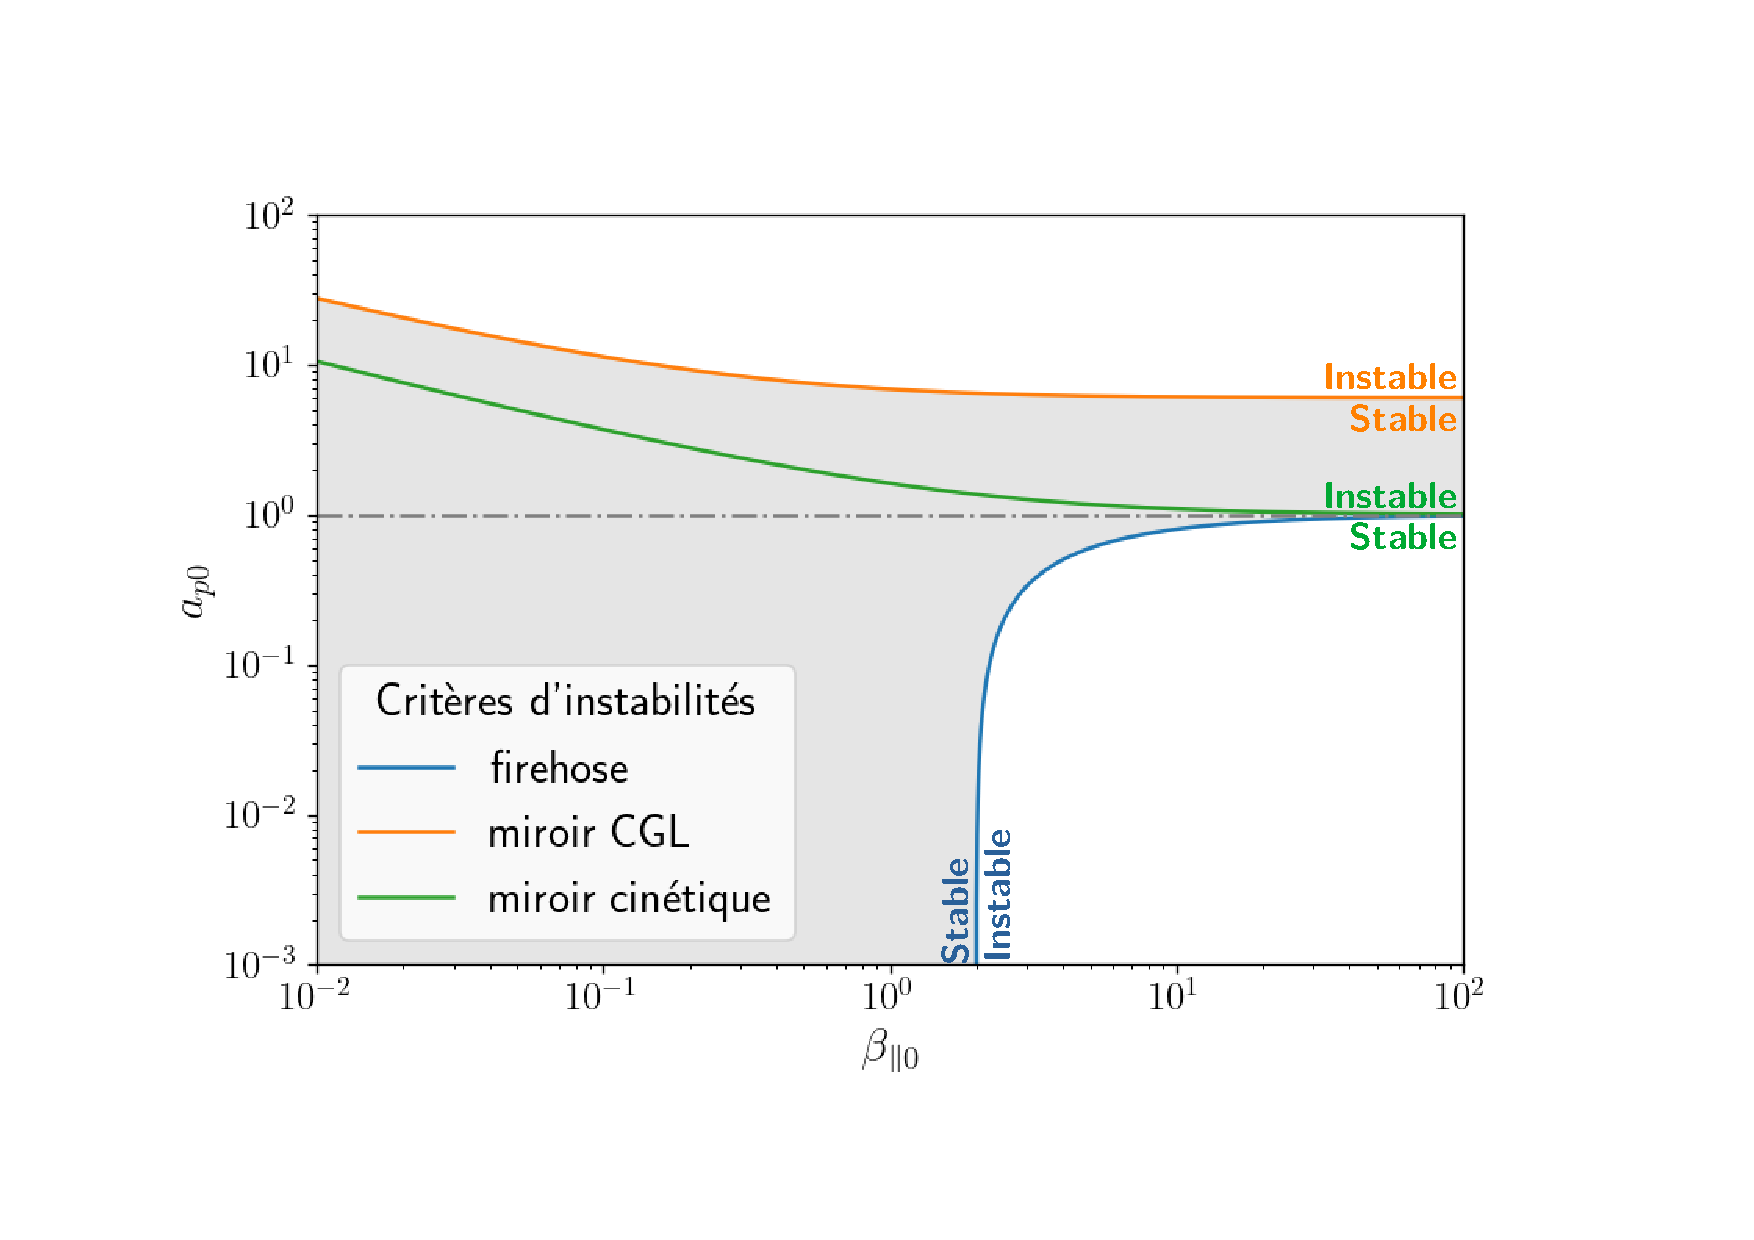
\includegraphics[width=0.9\linewidth,trim=3cm 2cm 4cm 3cm, clip=true]{./Mainmatter/Part_2/images/crit_diag_CGL}
\cprotect\caption{Zones de stabilité du modèle \cacro{CGL} (zone grisée). Critères d'instabilité firehose (bleu), miroir (orange) et miroir cinétique (vert). Horizontale \ensuremath{a_p=1} en gris.}
\label{fig:diag_cgl}
 \end{figure}
L'expression du critère d'instabilité miroir est légèrement différente de celle provenant de la théorie linéaire cinétique à cause du facteur $1/6$ [\cite{galeev_mhd_1983}, \cite{ferriere_mixed_2002}]. Ce facteur d'erreur translate la condition nécessaire pour qu'il y ait des instabilités miroir à $a_{p0}>6$ au lieu de $a_{p0}>1$, comme on peut le voir sur la \figref{fig:diag_cgl}. La condition nécessaire pour qu'il y ait apparition d'instabilité firehose est, quant à elle, $a_{p0}<1$ ce qui est en accord avec la théorie cinétique. Dans le vent solaire, ces critères d'instabilité semblent avoir un impact majeur puisque l'état du plasma semble maintenu, sur les diagrammes $a_p-\beta_{\parallel}$, dans une zone qu'ils semblent délimiter, comme l'a observé \cite{hellinger_solar_2006} dans les données relevées par la sonde \cacro{WIND}. 

Dans le Chapitre \ref{ch-11}, nous avons rappelé l'importance des ondes d'Alfvén dans les théories de turbulence et, dans le Chapitre \ref{ch-12}, que le sujet de l'impact des ondes compressibles \cacro{MHD} sur la cascade turbulente est toujours ouvert [\cite{brodiano_spatiotemporal_2021}]. Similairement, on peut se demander quel est l'impact des instabilités sur la turbulence ? Et en particulier, quelle est l'influence des instabilités des ondes d'Alfvén (firehose) sur la turbulence Alfvénique ? 

 Si l'on regarde les résultats des études de la température isotrope [\cite{liu_thermodynamic_2006}], des fluctuations magnétiques [\cite{bale_magnetic_2009}] et du taux de cascade incompressible [\cite{osman_proton_2013}] (voir \figref{fig:diag_osman}) dans les données relevées par \cacro{WIND} et ceux du taux compressible isotherme observés par \cite{hadid_compressible_2018} dans les données des missions \cacro{THEMIS} et \cacro{CLUSTER}, on remarque que sur les diagrammes $a_p-\beta_{\parallel}$, près des frontières des zones instables, la température des protons semble plus élevée, et les fluctuations du champ magnétique ainsi que les taux de cascade plus importants. Mais la relation entre instabilités et turbulence reste à clarifier : le plasma est-il plus chaud et turbulent parce que les instabilités jouent un rôle dans son chauffage ? Ce chauffage s'effectue-t-il via la cascade turbulente ? Ou est-ce lié à l'âge collisionnel du plasma comme le propose \cite{bale_magnetic_2009} ?
\begin{figure}[!ht]
 \centering
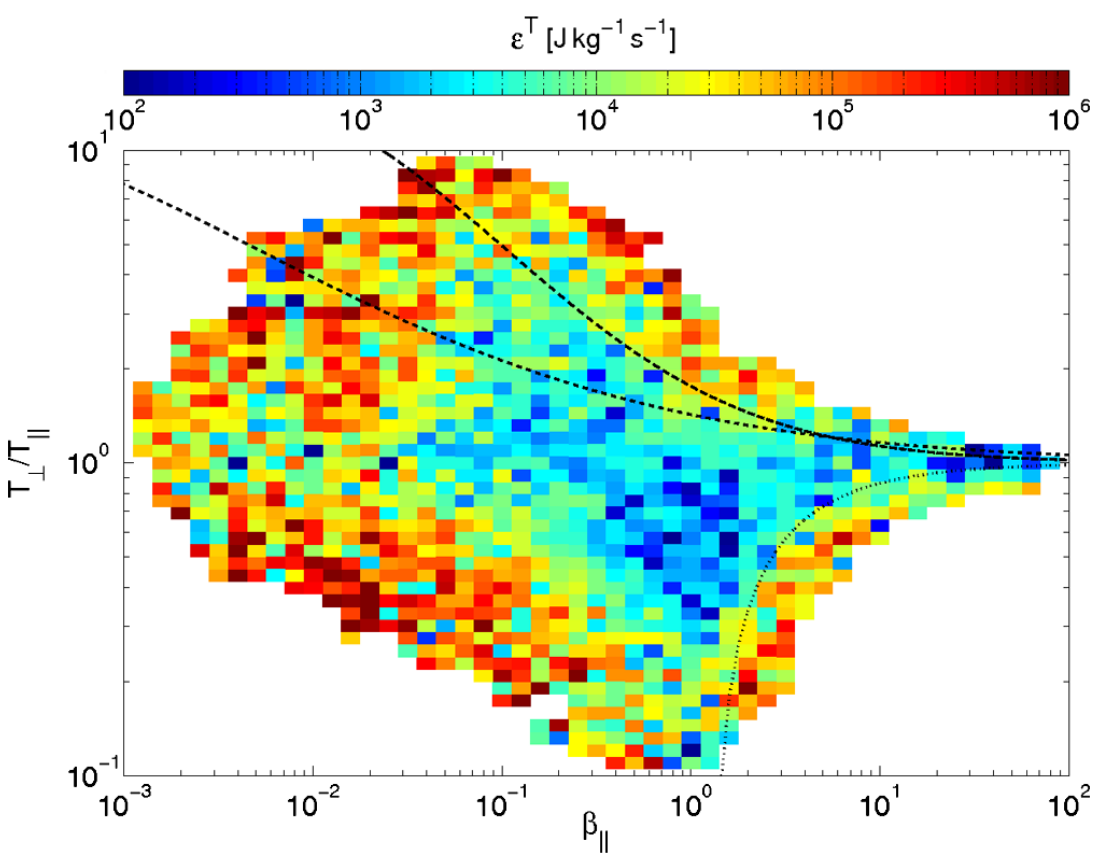
\includegraphics[width=0.8\linewidth,trim=0cm 0cm 0cm 0cm, clip=true]{./Mainmatter/Part_2/images/osman_2013}
\cprotect\caption{Distribution statistique en fonction de \ensuremath{a_p = \frac{p_{\perp}}{p_{\parallel}} =  \frac{T_{\perp}}{T_{\parallel}}} et \ensuremath{\beta_{\parallel}} d'échantillons relevés entre 1995 et 2011 dans le vent solaire par la sonde \cacro{WIND} en orbite autour de la Terre. Pour chacun d'eux, le taux de cascade est calculé avec la loi exacte \cacro{PP98} et indiqué par l'échelle chromatique. Les courbes pointillées indiquent les frontières associées aux instabilités cinétiques miroir (décroissante supérieure), cyclotron (décroissante inférieure) et firehose (croissante). [Crédits : \cite{osman_proton_2013}.]}
\label{fig:diag_osman}
\end{figure}

De multiples études se sont attaquées à ces questions à travers des comparaisons de spectres, du taux d'anisotropie de pression et des taux de croissance des instabilités cinétiques linéaires et quasi-linéaires. Parmi les plus récentes, on notera \cite{qudsi_intermittency_2020}, \cite{markovskii_effect_2022}, \cite{opie_conditions_2022}, \cite{bandyopadhyay_interplay_2022}, \cite{navarro_effects_2023}. 
De notre côté, nous l'attaquons analytiquement à partir des échelles fluides et de la théorie des lois exactes, dans le but d'offrir un cadre fluide permettant d'étudier plus rigoureusement l'impact des anisotropies et instabilités de pression sur la cascade turbulente.

\section{Loi exacte générale dépendant d'une pression tensorielle et loi CGL}
\label{sec-213}

Pour obtenir une loi exacte pour le modèle \ac{CGL}, nous avons utilisé la méthode mise en place dans le Chapitre \ref{ch-13}, c'est-à-dire prendre en compte l'équation d'énergie interne \eqref{eq:model_cpg_u} et non la forme explicite des pressions parallèle et perpendiculaire \eqref{eq:model_cpg_biadiab}. Le modèle utilisé est donc :
\begin{eqnarray}
\label{eq:turb_cpg_r} \partial_t \rho &=& - \nabla \cdot \left(\rho \boldsymbol{v}\right) , \\
\label{eq:turb_cpg_v}\partial_t  \boldsymbol{v} &=&- \nabla \cdot \left(\boldsymbol{v}\boldsymbol{v}\right) + \boldsymbol{v} \nabla \cdot \boldsymbol{v}  + \frac{1}{\rho} \nabla \cdot \left(\rho \boldsymbol{v_A}\boldsymbol{v_A}\right) - \frac{1}{\rho}  \nabla \cdot \overline{\boldsymbol{P_*}}  + \boldsymbol{f_c} + \boldsymbol{d_c} ,\\
\label{eq:turb_cpg_b}\partial_t \boldsymbol{v_A} &=&   \nabla \cdot \left(\boldsymbol{v_A}\boldsymbol{v} - \boldsymbol{v}\boldsymbol{v_A}\right) -  \boldsymbol{v}  \nabla \cdot \boldsymbol{v_A} +  \frac{\boldsymbol{v_A}}{2}  \nabla \cdot \boldsymbol{v} + \boldsymbol{f_m} + \boldsymbol{d_m} ,\\
\label{eq:turb_cpg_u}    \partial_t u  &=& - \nabla \cdot \left(u \boldsymbol{v} \right) + u  \nabla \cdot \boldsymbol{v}  -  \frac{\overline{\boldsymbol{P}}}{\rho} : \nabla \boldsymbol{v} . 
\end{eqnarray}

De manière cohérente avec les choix effectués dans le Chapitre \ref{ch-13}, la fonction de corrélation d'énergie totale choisie est $\mathcal{R} = \mathcal{R}_{c} + \mathcal{R}_{m} + \mathcal{R}_{u}$ avec $\mathcal{R}_{c} = \left<\frac{1}{4} \left(\rho'+\rho\right) \boldsymbol{v'} \cdot  \boldsymbol{v} \right>$, $\mathcal{R}_{m} = \left<\frac{1}{4} \left(\rho'+\rho\right) \boldsymbol{v'_A} \cdot  \boldsymbol{v_A} \right>$ et $\mathcal{R}_{u} = \frac{1}{2}\left< \rho' u + \rho u'\right> $. 

En appliquant la  même méthode que celle utilisée pour obtenir \eqref{eq:turb_cpi_Rc}, \eqref{eq:turb_cpi_Rm} et \eqref{eq:turb_cpi_Ru}, on obtient l'évolution temporelle des fonctions de corrélation associées à chaque énergie : 
\begin{itemize}
    \item Énergie cinétique : $\mathcal{R}_{c} = \left<\left(\rho'+\rho\right)\boldsymbol{v'} \cdot \boldsymbol{v}\right>/4 $
\begin{eqnarray}
\label{eq:turb_cpg_Rc} 4\partial_t \mathcal{R}_{c} &=& \nabla_{\boldsymbol{\ell}} \cdot \left<\delta \left(\rho\boldsymbol{v}\right) \cdot \delta \boldsymbol{v} \delta \boldsymbol{v} -\left(\delta \left(\rho\boldsymbol{v_A}\right) \cdot \delta \boldsymbol{v} \delta \boldsymbol{v_A} + \delta \left(\rho\boldsymbol{v}\right) \cdot \delta \boldsymbol{v_A} \delta \boldsymbol{v_A} \right)\right>\nonumber \\
&&+ \nabla_{\boldsymbol{\ell}} \cdot \left<\rho' \boldsymbol{v'_A}\cdot  \boldsymbol{v} \boldsymbol{v_A} -\rho \boldsymbol{v_A}\cdot  \boldsymbol{v'} \boldsymbol{v'_A}-\rho' \boldsymbol{v'} \cdot\boldsymbol{v_A}\boldsymbol{v'_A} +  \rho  \boldsymbol{v} \cdot\boldsymbol{v'_A}\boldsymbol{v_A}\right> \nonumber\\
& &+\left<\delta \boldsymbol{v}\cdot \left( \rho \boldsymbol{v}  \nabla' \cdot \boldsymbol{v'} -\rho' \boldsymbol{v'} \nabla \cdot \boldsymbol{v} \right)+2 \delta \boldsymbol{v_A}\cdot \left( \rho' \boldsymbol{v'} \nabla \cdot \boldsymbol{v_A} - \rho \boldsymbol{v} \right) \nabla' \cdot \boldsymbol{v'_A}\right> \nonumber\\
&&+  \nabla_{\boldsymbol{\ell}} \cdot \left< \rho' \frac{ \overline{\boldsymbol{P_*}}}{\rho} \cdot \boldsymbol{v'} -  \rho \frac{\overline{\boldsymbol{P'_*}}}{\rho'} \cdot \boldsymbol{v} + \overline{\boldsymbol{P_*}} \cdot \boldsymbol{v'} -  \overline{\boldsymbol{P'_*}} \cdot \boldsymbol{v} \right>\nonumber \\
&&- \left<\frac{\rho'}{\rho} \boldsymbol{v'} \cdot \overline{\boldsymbol{P_*}}  \cdot \frac{\nabla \rho}{\rho} + \frac{\rho}{\rho'} \boldsymbol{v} \cdot \overline{\boldsymbol{P'_*}}   \cdot \frac{\nabla' \rho'}{\rho'} \right>\nonumber\\
&&+  \left<\left(\rho' + \rho\right)\left(\boldsymbol{v} \cdot \boldsymbol{f'_c} + \boldsymbol{v'} \cdot \boldsymbol{f_c}\right) \right>+ \left<\left(\rho' + \rho\right)\left(\boldsymbol{v} \cdot \boldsymbol{d'_c} + \boldsymbol{v'} \cdot \boldsymbol{d_c}\right)\right> .
\end{eqnarray}
    \item Énergie magnétique : $\mathcal{R}_{m} = \left<\left(\rho'+\rho\right)\boldsymbol{v'_A} \cdot \boldsymbol{v_A}\right>/4 $
\begin{eqnarray}
\label{eq:turb_cpg_Rm} 4\partial_t \mathcal{R}_{m} &=& \nabla_{\boldsymbol{\ell}} \cdot \left<\delta \left(\rho\boldsymbol{v_A}\right) \cdot \delta \boldsymbol{v_A} \delta \boldsymbol{v} \right> \nonumber\\
&&-\nabla_{\boldsymbol{\ell}} \cdot \left< \rho' \boldsymbol{v'_A}\cdot  \boldsymbol{v} \boldsymbol{v_A} - \rho \boldsymbol{v_A}\cdot  \boldsymbol{v'} \boldsymbol{v'_A}-\rho' \boldsymbol{v'} \cdot\boldsymbol{v_A}\boldsymbol{v'_A} +  \rho  \boldsymbol{v} \cdot\boldsymbol{v'_A}\boldsymbol{v_A}\right> \nonumber\\
&&+ \left<\left(\rho \boldsymbol{v_A} \cdot \delta \boldsymbol{v_A} -\frac{1}{2} \left(\rho'+\rho\right) \boldsymbol{v'_A} \cdot \boldsymbol{v_A}\right)\nabla' \cdot \boldsymbol{v'}\right> \nonumber\\
&&-  \left<\left(\rho' \boldsymbol{v'_A} \cdot \delta \boldsymbol{v_A} + \frac{1}{2} \left(\rho'+\rho\right) \boldsymbol{v'_A} \cdot \boldsymbol{v_A}\right)\nabla \cdot \boldsymbol{v}\right>\nonumber\\
&& + \left<\left( \rho' \boldsymbol{v'_A} \cdot \boldsymbol{v} - \rho \boldsymbol{v} \cdot \boldsymbol{v'_A}  \right)\nabla \cdot \boldsymbol{v_A} \right> + \left<\left(\rho' \boldsymbol{v'} \cdot \boldsymbol{v_A} -  \rho \boldsymbol{v_A} \cdot \boldsymbol{v'} \right)\nabla' \cdot \boldsymbol{v'_A} \right>\nonumber\\
&&+  \left<\left(\rho' + \rho\right)\left(\boldsymbol{v_A} \cdot \boldsymbol{f'_m} + \boldsymbol{v'_A} \cdot \boldsymbol{f_m}\right) \right>+ \left<\left(\rho' + \rho\right)\left(\boldsymbol{v_A} \cdot \boldsymbol{d'_m} + \boldsymbol{v'_A} \cdot \boldsymbol{d_m}\right)\right> .\nonumber\\
\end{eqnarray}
    \item Énergie interne :  $\mathcal{R}_{u} = \left<\rho' u+\rho u'\right>/2 $
\begin{eqnarray}
\label{eq:turb_cpg_Ru} 2\partial_t \mathcal{R}_{u} &=&\nabla_{\boldsymbol{\ell}} \cdot \left<\delta \rho  \delta u \delta \boldsymbol{v} \right> + \left<  \rho \delta u \nabla' \cdot \boldsymbol{v'}- \rho' \delta u \nabla \cdot \boldsymbol{v}\right> \nonumber\\
&&-\left< \rho' \frac{\overline{\boldsymbol{P}}}{\rho} :  \nabla  \boldsymbol{v}  + \rho \frac{\overline{\boldsymbol{P'}}}{\rho'} : \nabla'  \boldsymbol{v'} \right> .
\end{eqnarray}
\end{itemize}
Le résultat pour l'énergie magnétique n'est pas influencé par le type de pression (tensoriel ou isotrope) contrairement à ceux des énergies cinétique et interne. La question qui s'est posée alors était : est-il possible d'améliorer la formulation des termes dépendant de la pression ? Autrement dit, est-il possible de faire apparaître l'influence de la pression dans les termes de type flux sous la forme d'une fonction de structure ?
 En remarquant que $\overline{\boldsymbol{P}}$ ou $\overline{\boldsymbol{P_*}}$ est, dans tous les termes, accompagné de $\frac{1}{\rho}$ pris au même point, l'idée de travailler sur la fonction de structure $\left<\delta \rho \delta \frac{ \overline{\boldsymbol{P}}}{\rho} \cdot \delta \boldsymbol{v} \right>$ puis sur la fonction $\left<\delta \rho \delta \frac{ \overline{\boldsymbol{P_*}} }{\rho} \cdot\delta \boldsymbol{v} \right>$ a émergé. Développer cette dernière sous la divergence locale en utilisant l'hypothèse d'homogénéité statistique et l'indépendance des positions $\boldsymbol{x}$ et  $\boldsymbol{x'}$ donne alors : 
\begin{eqnarray*}
    \nabla_{\boldsymbol{\ell}} \cdot \left<\delta \rho \delta \frac{ \overline{\boldsymbol{P_*}} }{\rho}  \cdot\delta \boldsymbol{v} \right> &=& \nabla_{\boldsymbol{\ell}} \cdot \left< \left[\rho  \frac{ \overline{\boldsymbol{P'_*}} }{\rho'}   \cdot\boldsymbol{v}  -\rho'  \frac{ \overline{\boldsymbol{P_*}} }{\rho} \cdot \boldsymbol{v'}\right] +  \left[\overline{\boldsymbol{P_*}} \cdot \boldsymbol{v'} - \overline{\boldsymbol{P'_*}}    \cdot\boldsymbol{v} \right] \right> \\
    &&+\nabla_{\boldsymbol{\ell}} \cdot \left<\rho'  \frac{ \overline{\boldsymbol{P_*}} }{\rho} \cdot \boldsymbol{v} - \rho  \frac{ \overline{\boldsymbol{P'_*}} }{\rho'}  \cdot \boldsymbol{v'}  \right> .
\end{eqnarray*}
 On peut donc exprimer $ \nabla_{\boldsymbol{\ell}} \cdot \left< \rho' \frac{ \overline{\boldsymbol{P_*}}}{\rho} \cdot \boldsymbol{v'} -  \rho \frac{\overline{\boldsymbol{P'_*}}}{\rho'} \cdot \boldsymbol{v} \right>$ ou $ \nabla_{\boldsymbol{\ell}} \cdot \left<  \overline{\boldsymbol{P_*}} \cdot \boldsymbol{v'} -  \overline{\boldsymbol{P'_*}} \cdot \boldsymbol{v} \right>$ en fonction de $\left<\delta \rho \delta \frac{ \overline{\boldsymbol{P_*}} }{\rho} \cdot\delta \boldsymbol{v} \right>$ dans \eqref{eq:turb_cpg_Rc}. Sachant que 
 \begin{equation*}
  \nabla_{\boldsymbol{\ell}} \cdot \left<  \overline{\boldsymbol{P_*}} \cdot \boldsymbol{v'} -  \overline{\boldsymbol{P'_*}} \cdot \boldsymbol{v} \right> = \left<  \rho  \frac{ \overline{\boldsymbol{P_*}} }{\rho} : \nabla'\boldsymbol{v'} +   \rho'\frac{ \overline{\boldsymbol{P'_*}} }{\rho'} : \nabla \boldsymbol{v} \right>
 \end{equation*}
 rappellant les termes dépendant de la pression dans l'équation \eqref{eq:turb_cpg_Ru}, nous avons choisi la première possibilité. Ainsi : 
\begin{eqnarray*}
\nabla_{\boldsymbol{\ell}} &\cdot& \left< \rho' \frac{ \overline{\boldsymbol{P_*}}}{\rho} \cdot \boldsymbol{v'} -  \rho \frac{\overline{\boldsymbol{P'_*}}}{\rho'} \cdot \boldsymbol{v}  +  \overline{\boldsymbol{P_*}} \cdot \boldsymbol{v'} -  \overline{\boldsymbol{P'_*}} \cdot \boldsymbol{v} \right>\\
&=& -\nabla_{\boldsymbol{\ell}} \cdot \left<\delta \rho \delta \frac{ \overline{\boldsymbol{P_*}} }{\rho} \cdot \delta \boldsymbol{v} \right> +  \left<   \boldsymbol{v}\cdot\frac{ \overline{\boldsymbol{P_*}} }{\rho} \cdot  \nabla'\rho' + \boldsymbol{v'} \cdot \frac{ \overline{\boldsymbol{P'_*}} }{\rho'} \cdot \nabla \rho  \right> \\
&&+ \left< 2 \rho  \frac{ \overline{\boldsymbol{P}} }{\rho} : \nabla'\boldsymbol{v'} + 2  \rho'\frac{ \overline{\boldsymbol{P'}} }{\rho'} : \nabla \boldsymbol{v}  + \rho \boldsymbol{v_A}^2 \nabla' \cdot \boldsymbol{v'} +   \rho' \boldsymbol{v'_A}^2 \nabla \cdot \boldsymbol{v}\right> .
\end{eqnarray*}

La loi \cacro{KHM} générale pour l'énergie totale avec $\mathcal{R} = \mathcal{R}_{c} + \mathcal{R}_{m} + \mathcal{R}_{u}$ devient alors :
\begin{equation}
\label{eq:turb_cpg_khm} \boxed{
\begin{array}{lcl}
{}_{[1]} \quad 4\partial_t \mathcal{R} &=& \nabla_{\boldsymbol{\ell}} \cdot \left<\left(\delta \left(\rho\boldsymbol{v}\right) \cdot \delta \boldsymbol{v}+ \delta \left(\rho\boldsymbol{v_A}\right) \cdot \delta \boldsymbol{v_A} \right) \delta \boldsymbol{v}  -\left(\delta \left(\rho\boldsymbol{v_A}\right) \cdot \delta \boldsymbol{v}  + \delta \left(\rho\boldsymbol{v}\right) \cdot \delta \boldsymbol{v_A}  \right) \delta \boldsymbol{v_A} \right>\\
{}_{[2]} && +\left< \left(\rho \boldsymbol{v} \cdot \delta \boldsymbol{v} +\frac{1}{2} \rho \boldsymbol{v_A} \cdot  \delta \boldsymbol{v_A} -\frac{1}{2} \delta \left(\rho \boldsymbol{v_A}\right) \cdot \boldsymbol{v_A} \right) \nabla' \cdot \boldsymbol{v'} \right>\\
{}_{[3]} && -\left< \left(\rho' \boldsymbol{v'} \cdot \delta \boldsymbol{v}  + \frac{1}{2} \rho' \boldsymbol{v'_A} \cdot \delta \boldsymbol{v_A}  - \frac{1}{2} \delta \left(\rho \boldsymbol{v_A}\right) \cdot \boldsymbol{v'_A}  \right)\nabla \cdot \boldsymbol{v}\right>\\
{}_{[4]} &&+ \left<\left(2 \rho' \boldsymbol{v'} \cdot \delta \boldsymbol{v_A}- \delta \left(\rho \boldsymbol{v}\right) \cdot \boldsymbol{v'_A} + \rho' \boldsymbol{v'_A} \cdot \delta \boldsymbol{v}  \right)\nabla \cdot \boldsymbol{v_A}\right>\\
{}_{[5]} &&- \left<\left(2\rho \boldsymbol{v} \cdot \delta \boldsymbol{v_A} - \delta \left(\rho \boldsymbol{v}\right) \cdot \boldsymbol{v_A} +  \rho \boldsymbol{v_A} \cdot \delta \boldsymbol{v} \right)\nabla' \cdot \boldsymbol{v'_A}\right> \\
{}_{[6]} &&+ \nabla_{\boldsymbol{\ell}} \cdot \left< 2\delta \rho  \delta u \delta \boldsymbol{v}\right> + 2\left<\rho \delta u \nabla' \cdot \boldsymbol{v'}- \rho' \delta u \nabla \cdot \boldsymbol{v}\right>\\
{}_{[7]} &&- \nabla_{\boldsymbol{\ell}} \cdot \left<\delta \rho \delta \frac{ \overline{\boldsymbol{P_*}} }{\rho} \cdot \delta \boldsymbol{v} \right> - 2\left<\rho \delta \frac{ \overline{\boldsymbol{P}} }{\rho}:\nabla' \boldsymbol{v'} -  \rho' \delta \frac{ \overline{\boldsymbol{P}} }{\rho} :\nabla  \boldsymbol{v} \right>\\
{}_{[8]} && +  \left< \boldsymbol{v} \cdot \left(  \frac{ \overline{\boldsymbol{P_*}} }{\rho} \delta \rho - \rho \delta \frac{ \overline{\boldsymbol{P_*}} }{\rho}  \right)\cdot  \frac{\nabla' \rho'}{\rho'} - \boldsymbol{v'} \cdot \left(  \frac{ \overline{\boldsymbol{P'_*}} }{\rho'} \delta \rho - \rho' \delta \frac{ \overline{\boldsymbol{P_*}} }{\rho}  \right)\cdot  \frac{\nabla \rho}{\rho}  \right>\\
{}_{[9]}&&+  \left<\left(\rho' + \rho\right)\left(\boldsymbol{v} \cdot \boldsymbol{f'_c} + \boldsymbol{v'} \cdot \boldsymbol{f_c} + \boldsymbol{v_A} \cdot \boldsymbol{f'_m} + \boldsymbol{v'_A} \cdot \boldsymbol{f_m}\right) \right>\\
{}_{[10]}&&+ \left<\left(\rho' + \rho\right)\left(\boldsymbol{v} \cdot \boldsymbol{d'_c} + \boldsymbol{v'} \cdot \boldsymbol{d_c}+\boldsymbol{v_A} \cdot \boldsymbol{d'_m} + \boldsymbol{v'_A} \cdot \boldsymbol{d_m}\right)\right> .
\end{array}}
\end{equation} 
 Les lignes [7] et [8] contiennent les contributions des tenseurs de pression et de pression totale. 
 
La loi exacte générale de type \cacro{K41} est alors : 
\begin{equation}
\label{eq:turb_cpg_elk} \boxed{
\begin{array}{lcl}
- 4\varepsilon &=& \nabla_{\boldsymbol{\ell}} \cdot \left<\left(\delta \left(\rho\boldsymbol{v}\right) \cdot \delta \boldsymbol{v}+ \delta \left(\rho\boldsymbol{v_A}\right) \cdot \delta \boldsymbol{v_A} \right) \delta \boldsymbol{v}  -\left(\delta \left(\rho\boldsymbol{v_A}\right) \cdot \delta \boldsymbol{v}  + \delta \left(\rho\boldsymbol{v}\right) \cdot \delta \boldsymbol{v_A}  \right) \delta \boldsymbol{v_A} \right>\\
&&+ \nabla_{\boldsymbol{\ell}} \cdot \left< 2\delta \rho  \delta u \delta \boldsymbol{v}-\delta \rho \delta \frac{ \overline{\boldsymbol{P_*}} }{\rho} \cdot \delta \boldsymbol{v} \right> \\
&& +\left< \left(\rho \boldsymbol{v} \cdot \delta \boldsymbol{v} +\frac{1}{2} \rho \boldsymbol{v_A} \cdot  \delta \boldsymbol{v_A} -\frac{1}{2} \delta \left(\rho \boldsymbol{v_A}\right) \cdot \boldsymbol{v_A} +2\rho \delta u\right) \nabla' \cdot \boldsymbol{v'} -2\rho \delta \frac{ \overline{\boldsymbol{P}} }{\rho}:\nabla' \boldsymbol{v'}\right>\\
 && -\left< \left(\rho' \boldsymbol{v'} \cdot \delta \boldsymbol{v}  + \frac{1}{2} \rho' \boldsymbol{v'_A} \cdot \delta \boldsymbol{v_A}  - \frac{1}{2} \delta \left(\rho \boldsymbol{v_A}\right) \cdot \boldsymbol{v'_A}  +2\rho' \delta u\right)\nabla \cdot \boldsymbol{v} - 2\rho' \delta \frac{ \overline{\boldsymbol{P}} }{\rho} :\nabla  \boldsymbol{v}\right>\\
&&+ \left<\left(2 \rho' \boldsymbol{v'} \cdot \delta \boldsymbol{v_A}- \delta \left(\rho \boldsymbol{v}\right) \cdot \boldsymbol{v'_A} + \rho' \boldsymbol{v'_A} \cdot \delta \boldsymbol{v}  \right)\nabla \cdot \boldsymbol{v_A}\right>\\
 &&- \left<\left(2\rho \boldsymbol{v} \cdot \delta \boldsymbol{v_A} - \delta \left(\rho \boldsymbol{v}\right) \cdot \boldsymbol{v_A} +  \rho \boldsymbol{v_A} \cdot \delta \boldsymbol{v} \right)\nabla' \cdot \boldsymbol{v'_A}\right> \\
&& +  \left< \boldsymbol{v} \cdot \left(  \frac{ \overline{\boldsymbol{P_*}} }{\rho} \delta \rho - \rho \delta \frac{ \overline{\boldsymbol{P_*}} }{\rho}  \right)\cdot  \frac{\nabla' \rho'}{\rho'} - \boldsymbol{v'} \cdot \left(  \frac{ \overline{\boldsymbol{P'_*}} }{\rho'} \delta \rho - \rho' \delta \frac{ \overline{\boldsymbol{P_*}} }{\rho}  \right)\cdot  \frac{\nabla \rho}{\rho}  \right>.
\end{array}}
\end{equation}
Cette loi est valable quelle que soit la forme du tenseur de pression ou de l'énergie interne tant que la zone inertielle est supposée isentrope. Si l'on considère la pression sous forme isotrope $\overline{\boldsymbol{P}} = p \overline{\boldsymbol{I}}$, on trouve la loi \eqref{eq:turb_elg_f2} analysée dans la section \ref{sec-132}. On notera ce résultat $\varepsilon_{iso}$. On peut alors isoler dans le taux de cascade la contribution de la composante anisotrope du tenseur de pression $\overline{\boldsymbol{\Pi}}$ : 
\begin{equation}
\label{eq:turb_cpgyr_an} \boxed{
\begin{array}{lcl}
- 4\left(\varepsilon - \varepsilon_{iso}\right) &=& - \nabla_{\boldsymbol{\ell}} \cdot \left< \delta \rho \delta \left(\frac{\overline{\boldsymbol{\Pi}}}{\rho}\right) \cdot \delta \boldsymbol{v} \right>  -\left< 2\rho \delta \left(\frac{\overline{\boldsymbol{\Pi}}}{\rho}\right):\nabla' \boldsymbol{v'} -  2\rho' \delta \left(\frac{\overline{\boldsymbol{\Pi}}}{\rho}\right) :\nabla  \boldsymbol{v}\right>\\
&& +  \left< \boldsymbol{v} \cdot \left(  \left(\frac{\overline{\boldsymbol{\Pi}}}{\rho}\right) \delta \rho - \rho \delta \left(\frac{\overline{\boldsymbol{\Pi}}}{\rho}\right)  \right)\cdot  \frac{\nabla' \rho'}{\rho'}-\boldsymbol{v'} \cdot \left(  \left(\frac{\overline{\boldsymbol{\Pi'}}}{\rho'}\right) \delta \rho - \rho' \delta \left(\frac{\overline{\boldsymbol{\Pi}}}{\rho}\right)  \right)\cdot  \frac{\nabla \rho}{\rho}  \right>.
\end{array}}
\end{equation}
Nous quantifierons et analyserons cette contribution grâce à des simulations dans la Partie \ref{part_3}. 

Dans le cas d'un tenseur de pression gyrotrope, on peut faire apparaître $p_{\parallel}$ et $p_{\perp}$ : 
\begin{equation}
\label{eq:turb_cpgyr_elk}% \boxed{
\begin{array}{lcl}
%\begin{eqnarray}
%\label{eq:turb_cpgyr_elk} 
- 4\varepsilon &=& \nabla_{\boldsymbol{\ell}} \cdot \left<\left(\delta \left(\rho\boldsymbol{v}\right) \cdot \delta \boldsymbol{v}+ \delta \left(\rho\boldsymbol{v_A}\right) \cdot \delta \boldsymbol{v_A} \right)\delta \boldsymbol{v}  -\left(\delta \left(\rho\boldsymbol{v_A}\right) \cdot \delta \boldsymbol{v}  + \delta \left(\rho\boldsymbol{v}\right) \cdot \delta \boldsymbol{v_A}  \right) \delta \boldsymbol{v_A} \right>\\
&+& \nabla_{\boldsymbol{\ell}} \cdot \left< \delta \rho  \delta \left(\frac{p_{\perp} + p_{\parallel}+p_m}{\rho}\right) \delta \boldsymbol{v}+\delta \rho \delta \left(\frac{p_{\perp} - p_{\parallel}}{\rho}\boldsymbol{b}\boldsymbol{b}\right) \cdot \delta \boldsymbol{v} \right> \\
& +&\left< \left(\rho \boldsymbol{v} \cdot \delta \boldsymbol{v} +\frac{1}{2} \rho \boldsymbol{v_A} \cdot  \delta \boldsymbol{v_A} -\frac{1}{2} \delta \left(\rho \boldsymbol{v_A}\right) \cdot \boldsymbol{v_A} +\rho \delta \left(\frac{p_{\parallel}}{\rho}\right)\right) \nabla' \cdot \boldsymbol{v'} \right>\\
 & -&\left< \left(\rho' \boldsymbol{v'} \cdot \delta \boldsymbol{v}  + \frac{1}{2} \rho' \boldsymbol{v'_A} \cdot \delta \boldsymbol{v_A}  - \frac{1}{2} \delta \left(\rho \boldsymbol{v_A}\right) \cdot \boldsymbol{v'_A}  +\rho' \delta \left(\frac{p_{\parallel}}{\rho}\right)\right)\nabla \cdot \boldsymbol{v} \right>\\
 &+&2\left<\rho \delta \left(\frac{p_{\perp} - p_{\parallel}}{\rho}\boldsymbol{b}\boldsymbol{b}\right):\nabla' \boldsymbol{v'} - \rho' \delta \left(\frac{p_{\perp} - p_{\parallel}}{\rho}\boldsymbol{b}\boldsymbol{b}\right) :\nabla  \boldsymbol{v}\right>\\
&+& \left<\left(2 \rho' \boldsymbol{v'} \cdot \delta \boldsymbol{v_A}- \delta \left(\rho \boldsymbol{v}\right) \cdot \boldsymbol{v'_A} + \rho' \boldsymbol{v'_A} \cdot \delta \boldsymbol{v}  \right)\nabla \cdot \boldsymbol{v_A}\right>\\
 &-& \left<\left(2\rho \boldsymbol{v} \cdot \delta \boldsymbol{v_A} - \delta \left(\rho \boldsymbol{v}\right) \cdot \boldsymbol{v_A} +  \rho \boldsymbol{v_A} \cdot \delta \boldsymbol{v} \right)\nabla' \cdot \boldsymbol{v'_A}\right>\\
   %& +&  \left< \delta \rho  \left( \left( \frac{p_{\perp}+p_m }{\rho} \boldsymbol{v} +  \frac{ p_{\parallel}-p_{\perp}}{\rho} \boldsymbol{v} \cdot\boldsymbol{b}\boldsymbol{b}   \right)\cdot  \frac{\nabla' \rho'}{\rho'} - \left(\frac{ p'_{\perp}+p'_m }{\rho'} \boldsymbol{v'}+ \frac{ p'_{\parallel}-p'_{\perp}}{\rho'}\boldsymbol{v'} \cdot\boldsymbol{b'}\boldsymbol{b'}\right)\cdot  \frac{\nabla \rho}{\rho}\right)   \right>\nonumber \\
   %- \delta \left(\frac{ p_{\perp}+p_m }{\rho}\right) \left(\rho \boldsymbol{v} \cdot  \frac{\nabla' \rho'}{\rho'} -  \rho' \boldsymbol{v'}\cdot  \frac{\nabla \rho}{\rho}\right)  \right>\nonumber \\
  % &+& \left<  \delta \rho\left( \frac{ p_{\parallel}-p_{\perp}}{\rho} \boldsymbol{v} \cdot\boldsymbol{b}\boldsymbol{b}   \cdot  \frac{\nabla' \rho'}{\rho'} - \frac{ p'_{\parallel}-p'_{\perp}}{\rho'}\boldsymbol{v'} \cdot\boldsymbol{b'}\boldsymbol{b'}  \cdot  \frac{\nabla \rho}{\rho}\right)
  % -  \delta \left(\frac{ p_{\parallel}-p_{\perp}}{\rho}\boldsymbol{b}\boldsymbol{b} \right) : \left( \rho  \boldsymbol{v}  \frac{\nabla' \rho'}{\rho'} - \rho' \boldsymbol{v'}   \frac{\nabla \rho}{\rho} \right)\right>\nonumber \\
  & +&  \left<  \left(  \frac{p_{\perp}+p_m }{\rho} \boldsymbol{v}\delta \rho - \rho \boldsymbol{v}\delta \left(\frac{ p_{\perp}+p_m }{\rho}\right) \right)\cdot  \frac{\nabla' \rho'}{\rho'} \right>\\
  &+&  \left<  \left(    \frac{ p_{\parallel}-p_{\perp}}{\rho} \boldsymbol{v} \cdot\boldsymbol{b}\boldsymbol{b} \delta \rho -\rho  \boldsymbol{v} \cdot \delta \left(\frac{ p_{\parallel}-p_{\perp}}{\rho}\boldsymbol{b}\boldsymbol{b} \right)  \right)\cdot  \frac{\nabla' \rho'}{\rho'} \right>\\
 &-& \left< \left(  \frac{ p'_{\perp}+p'_m }{\rho'} \boldsymbol{v'}\delta \rho - \rho' \boldsymbol{v'}\delta \left(\frac{ p_{\perp}+p_m }{\rho}\right) \right) \cdot  \frac{\nabla \rho}{\rho} \right>\\
 &-&   \left< \left(  \frac{ p'_{\parallel}-p'_{\perp}}{\rho'}\boldsymbol{v'} \cdot\boldsymbol{b'}\boldsymbol{b'}  \delta \rho - \rho' \boldsymbol{v'} \cdot\delta \left(\frac{ p_{\parallel}-p_{\perp}}{\rho}\boldsymbol{b}\boldsymbol{b} \right)\right) \cdot  \frac{\nabla \rho}{\rho} \right> .
%\end{eqnarray}
\end{array}%}
\end{equation}
Cette loi est valable pour le modèle \cacro{CGL}. Si besoin est, on peut y expliciter $p_{\parallel}$ et $p_{\perp}$ en fonction de $\rho$, $\boldsymbol{v_A}$ grâce à \eqref{eq:model_cpg_biadiab}. 

On peut aussi faire apparaître $a_p$ et $\beta_{\parallel}$ dans \eqref{eq:turb_cpgyr_elk} pour identifier les termes potentiellement impactés par les instabilités. Ainsi, on obtient :  
\begin{equation}
\label{eq:turb_cpinst_elk} \boxed{
\begin{array}{lcl}
- 4\varepsilon &=& \nabla_{\boldsymbol{\ell}} \cdot \left<\left(\delta \left(\rho\boldsymbol{v}\right) \cdot \delta \boldsymbol{v}+ \delta \left(\rho\boldsymbol{v_A}\right) \cdot \delta \boldsymbol{v_A} \right) \delta \boldsymbol{v}  -\left(\delta \left(\rho\boldsymbol{v_A}\right) \cdot \delta \boldsymbol{v}  + \delta \left(\rho\boldsymbol{v}\right) \cdot \delta \boldsymbol{v_A}  \right) \delta \boldsymbol{v_A} \right>\\
&&+ \frac{1}{2}\nabla_{\boldsymbol{\ell}} \cdot \left< \delta \rho  \delta \left(\boldsymbol{v_A}^2 \left(\beta_{\parallel}\left(a_p+1\right)+1\right)\right) \delta \boldsymbol{v}+\delta \rho \delta \left(\beta_{\parallel}\left(a_p-1\right) \boldsymbol{v_A} \boldsymbol{v_A}\right) \cdot \delta \boldsymbol{v} \right> \\
&& +\left< \left(\rho \boldsymbol{v} \cdot \delta \boldsymbol{v} +\frac{1}{2} \rho \boldsymbol{v_A} \cdot  \delta \boldsymbol{v_A} -\frac{1}{2} \delta \left(\rho \boldsymbol{v_A}\right) \cdot \boldsymbol{v_A} + \frac{1}{2}\rho \delta \left(\boldsymbol{v_A}^2 \beta_{\parallel}\right)\right) \nabla' \cdot \boldsymbol{v'} \right>\\
 && -\left< \left(\rho' \boldsymbol{v'} \cdot \delta \boldsymbol{v}  + \frac{1}{2} \rho' \boldsymbol{v'_A} \cdot \delta \boldsymbol{v_A}  - \frac{1}{2} \delta \left(\rho \boldsymbol{v_A}\right) \cdot \boldsymbol{v'_A}  + \frac{1}{2} \rho' \delta \left(\boldsymbol{v_A}^2 \beta_{\parallel}\right)\right)\nabla \cdot \boldsymbol{v} \right>\\
 &&+\left<\rho \delta \left(\beta_{\parallel}\left(a_p-1\right) \boldsymbol{v_A} \boldsymbol{v_A}\right):\nabla' \boldsymbol{v'} - \rho' \delta \left(\beta_{\parallel}\left(a_p-1\right) \boldsymbol{v_A} \boldsymbol{v_A}\right) :\nabla  \boldsymbol{v}\right>\\
&&+ \left<\left(2 \rho' \boldsymbol{v'} \cdot \delta \boldsymbol{v_A}- \delta \left(\rho \boldsymbol{v}\right) \cdot \boldsymbol{v'_A} + \rho' \boldsymbol{v'_A} \cdot \delta \boldsymbol{v}  \right)\nabla \cdot \boldsymbol{v_A}\right>\\
 &&- \left<\left(2\rho \boldsymbol{v} \cdot \delta \boldsymbol{v_A} - \delta \left(\rho \boldsymbol{v}\right) \cdot \boldsymbol{v_A} +  \rho \boldsymbol{v_A} \cdot \delta \boldsymbol{v} \right)\nabla' \cdot \boldsymbol{v'_A}\right> \\
&& + \frac{1}{2} \left<  \left(  \boldsymbol{v_A}^2 \left(\beta_{\parallel}a_p+1\right) \delta \rho - \rho \delta \left(\boldsymbol{v_A}^2 \left(\beta_{\parallel}a_p+1\right)\right)  \right)\boldsymbol{v}\cdot  \frac{\nabla' \rho'}{\rho'} \right>\\
&&- \frac{1}{2} \left<\left(  \boldsymbol{v'_A}^2 \left(\beta'_{\parallel}a'_p+1\right) \delta \rho - \rho' \delta \left(\boldsymbol{v_A}^2 \left(\beta_{\parallel}a_p+1\right)\right)  \right) \boldsymbol{v'}\cdot  \frac{\nabla \rho}{\rho}  \right> \\
&& + \frac{1}{2} \left< \boldsymbol{v} \cdot \left(  \beta_{\parallel}\left(a_p-1\right) \boldsymbol{v_A} \boldsymbol{v_A} \delta \rho - \rho \delta \left(\beta_{\parallel}\left(a_p-1\right) \boldsymbol{v_A} \boldsymbol{v_A}\right)  \right)\cdot  \frac{\nabla' \rho'}{\rho'} \right>\\
&&-\frac{1}{2}\left< \boldsymbol{v'} \cdot \left( \beta'_{\parallel}\left(a'_p-1\right) \boldsymbol{v'_A} \boldsymbol{v'_A}  \delta \rho - \rho' \delta \left(\beta_{\parallel}\left(a_p-1\right) \boldsymbol{v_A} \boldsymbol{v_A} \right)\right) \cdot  \frac{\nabla \rho}{\rho} \right>.
\end{array}}
\end{equation}
Les critères d'instabilité linéaires n'y sont pas explicites, mais on observe que certains termes, présents dans la contribution anisotrope \eqref{eq:turb_cpgyr_an}, dépendent de $a_p-1$, en particulier le terme de type flux. Par conséquent, le signe de ces termes va dépendre du régime de pression dans le système, c'est-à-dire si $p_{\parallel}$ ou $p_{\perp}$ domine, et est ainsi lié au type d'instabilité pouvant s'y développer. Comme ces termes dépendent de quantités incrémentales, il est néanmoins difficile de conclure sur leur apport au taux de cascade total sans regarder dans des simulations. Ce sera l'un des objectifs de la Partie \ref{part_3}.

\newpage
\section{Synthèse de l'étude analytique de turbulence compressible avec pression tensorielle et modèle CGL}
\label{synt-21}

 \fcolorbox{blue}{white}{\begin{minipage}[c]{\linewidth}
 \paragraph{Fermeture CGL : } $\nabla \cdot \overline{\overline{\boldsymbol{q}}}=0$ et $\overline{\boldsymbol{P}}  = p \overline{\boldsymbol{I}} + \overline{\boldsymbol{\Pi}}=  \frac{2 p_{\perp} + p_{\parallel}}{3}  \overline{\boldsymbol{I}} + \left(p_{\parallel} - p_{\perp}\right)\left(\boldsymbol{b}\boldsymbol{b} - \frac{1}{3} \overline{\boldsymbol{I}} \right)$ avec $\boldsymbol{b} = \frac{\boldsymbol{v_A}}{|\boldsymbol{v_A}|}$. Energie interne définie telle que $\rho u = \frac{3}{2}p$.
\begin{eqnarray}
 \label{eq:synth_turbg_ppar}     \partial_t p_{\parallel} + \nabla \cdot \left(p_{\parallel} \boldsymbol{v} \right) + 2 p_{\parallel} \boldsymbol{b}\boldsymbol{b} : \nabla \boldsymbol{v}   &=& 0 ,\\
 \label{eq:synth_turbg_pperp}     \partial_t p_{\perp} + \nabla \cdot \left(p_{\perp} \boldsymbol{v} \right) + p_{\perp} \nabla \cdot \boldsymbol{v}- p_{\perp} \boldsymbol{b}\boldsymbol{b} : \nabla \boldsymbol{v}   &=& 0 .
 \end{eqnarray}
 
 \paragraph{Linéarisation du modèle CGL : }
 \begin{itemize}
     \item Relation de dispersion : \eqref{eq:lin_cpg_disp}
    \item Mode d'Alfvén incompressible $\Rightarrow$ instabilité firehose,
    \item Mode magnétosonore rapide : stable,
    \item Mode magnétosonore lent $\Rightarrow$ instabilité firehose parallèle et miroir
    \item instabilité firehose si $1-\frac{\beta_{\parallel 0}}{2} \left(1-a_{p0}\right)<0$
    \item instabilité miroir si $1+\beta_{\parallel 0}a_{p0}\left(1-\frac{1}{6}a_{p0}\right)<0$
\end{itemize}
\end{minipage}}

 \fcolorbox{red}{white}{\begin{minipage}[c]{\linewidth}
 \paragraph{Equations utilisées pour calculer la loi exacte générale avec tenseur de pression (zone inertielle isentrope) : }
\begin{eqnarray}
\label{eq:synth_turbg_r} \partial_t \rho &=& - \nabla \cdot \left(\rho \boldsymbol{v}\right),  \\
\label{eq:synth_turbg_v}\partial_t  \boldsymbol{v} &=&- \nabla \cdot \left(\boldsymbol{v}\boldsymbol{v}\right) + \boldsymbol{v} \nabla \cdot \boldsymbol{v}  + \frac{1}{\rho} \nabla \cdot \left(\rho \boldsymbol{v_A}\boldsymbol{v_A}\right) - \frac{1}{\rho}  \nabla \cdot \overline{\boldsymbol{P_*}}  + \left(\boldsymbol{f_c} + \boldsymbol{d_c}\right) ,\\
\label{eq:synth_turbg_b}\partial_t \boldsymbol{v_A} &=&   \nabla \cdot \left(\boldsymbol{v_A}\boldsymbol{v} - \boldsymbol{v}\boldsymbol{v_A}\right) -  \boldsymbol{v}  \nabla \cdot \boldsymbol{v_A} +  \frac{\boldsymbol{v_A}}{2}  \nabla \cdot \boldsymbol{v} + \left(\boldsymbol{f_m} + \boldsymbol{d_m}\right), \\
\label{eq:synth_turbg_u}    \partial_t u  &=& - \nabla \cdot \left(u \boldsymbol{v} \right) + u  \nabla \cdot \boldsymbol{v}  -  \frac{\overline{\boldsymbol{P}}}{\rho} : \nabla \boldsymbol{v}  .
\end{eqnarray}
 
 \paragraph{Fonctions de corrélation d'énergie totale considérée :}  
 \begin{equation*}\mathcal{R} = \frac{1}{2} \left<\frac{1}{2} \left(\rho'+\rho\right) \boldsymbol{v'} \cdot  \boldsymbol{v} + \frac{1}{2} \left(\rho'+\rho\right) \boldsymbol{v'_A} \cdot  \boldsymbol{v_A} +  \rho' u + \rho u' \right>.
 \end{equation*}

\paragraph{Lois exactes générales dérivées dans ce chapitre (formulation f2) :} 
\begin{itemize}
    \item \cacro{KHM} générale $\forall \overline{\boldsymbol{P}}$ :  \eqref{eq:turb_cpg_khm},
    \item \cacro{K41} générale $\forall \overline{\boldsymbol{P}}$ :  \eqref{eq:turb_cpg_elk},
    \item contribution de l'anisotropie de pression :  \eqref{eq:turb_cpgyr_an}.
\end{itemize}
\paragraph{Lois exactes K41 gyrotrope/CGL répondant à l'objectif initial (formulation f2) :} 
\begin{itemize}
    \item fonction de $p_{\parallel}$ et $p_{\perp}$ : \eqref{eq:turb_cpgyr_elk},
    \item fonction de $a_p = \frac{p_{\perp}}{p_{\parallel}}$ et $\beta_{\parallel} = \frac{p_{\parallel}}{p_m}$ : \eqref{eq:turb_cpinst_elk}.
\end{itemize}

Les résultats dérivés ici sont publiés dans \cite{simon_exact_2022}. 
\end{minipage}}


\chapitre{Et dans le cas incompressible ?}{ch-22}
\chapter{Et dans le cas incompressible ? }
\renewcommand\partie{\Partie\ Chapitre \thechapter}
\label{ch-22}

\bigskip
\minitoc  

Si l'on prend la limite incompressible de la loi exacte dépendant d'une pression isotrope \eqref{eq:turb_elg_f2}, on retrouve la loi \acs{PP98} donnant le taux de cascade $\varepsilon_{PP98}$ \eqref{eq:synth_inc_EL}. Mais est-ce aussi le cas si la pression est tensorielle ? De cette question émerge une autre question : qu'est-ce qu'un système incompressible avec pression tensorielle ? Dans ce chapitre, sera présenté le travail effectué pour tenter de répondre à ces questions. Ce travail n'a pas encore été publié. 

\section{De la limite incompressible dans la loi exacte générale vers un nouveau modèle }
\label{sec-221}

Si l'on considère la limite incompressible ($\rho = \rho_0$, $\delta \rho = 0$, $\nabla \rho=0$, $\nabla \cdot \boldsymbol{v}=0$, $\nabla \cdot \boldsymbol{v_A}=0$) dans l'équation \eqref{eq:turb_cpgyr_an}, $\varepsilon_{iso}$ devient $\varepsilon_{PP98}$ et tous les termes s'annulent sauf : 
\begin{eqnarray}
\label{eq:turb_cpinc_an} 
- 4(\varepsilon - \varepsilon_{PP98}) &=& -2 \left< \delta (\overline{\boldsymbol{\Pi}}):\nabla' \boldsymbol{v'} -   \delta (\overline{\boldsymbol{\Pi}} ) :\nabla  \boldsymbol{v}\right> 
\end{eqnarray}
car la contribution de la trace de $\nabla \boldsymbol{v}$ s'annule par incompressibilité : $\overline{\boldsymbol{I}} :\nabla \boldsymbol{v} = \nabla \cdot \boldsymbol{v}=0$. On obtient ainsi une correction à la théorie PP98 dépendant de la composante anisotrope de la pression (participant à la déformation incompressible du plasma, pour plus d'information voir [\cite{cassak_pressure-strain_2022}]) : 
\begin{equation}
\label{eq:turb_cpinc_gen} \boxed{
\begin{array}{lcl}
- 4(\varepsilon - \varepsilon_{PP98}) &=& -2 \left< \delta (\overline{\boldsymbol{P}} - p \overline{\boldsymbol{I}}):\delta (\nabla \boldsymbol{v}) \right> = -2 \left< \delta \overline{\boldsymbol{\Pi}} :\delta (\nabla \boldsymbol{v}) \right>.
\end{array}}
\end{equation}
Une question émerge de ce résultat : dans des plasmas faiblement compressibles dépendant d'une pression tensorielle tels que le vent solaire, la correction anisotrope aurait-elle plus de poids que la prise en compte de la compression via les fluctuations de densité ?

Dans le cas particulier gyrotrope, on obtient :
\begin{eqnarray}
\label{eq:turb_cpinc_gyr1} 
- 4(\varepsilon - \varepsilon_{PP98}) &=& -2 \left< \delta ((p_{\parallel} - p_{\perp})(\boldsymbol{b}\boldsymbol{b} -\frac{1}{3} \overline{\boldsymbol{I}})):\delta (\nabla \boldsymbol{v}) \right> \\
\label{eq:turb_cpinc_gyr2} &=& -2 \left< \delta ((p_{\parallel} - p_{\perp})\boldsymbol{b}\boldsymbol{b}):\delta (\nabla \boldsymbol{v}) \right> .
\end{eqnarray}
On observe que la ligne \eqref{eq:turb_cpinc_gyr1} dépend de $\overline{\boldsymbol{I}} :\nabla \boldsymbol{v}$, on annule donc ce terme dans la ligne suivante \eqref{eq:turb_cpinc_gyr2}. Dans le cas incompressible, ces deux expressions sont donc équivalentes. Dans des plasmas quasi-incompressibles par contre, si l'on veut estimer le taux de cascade à l'aide de la loi exacte incompressible corrigée, les deux expressions ne seront plus équivalentes. Dans la première, on s'assure de n'utiliser que la part incompressible de la pression (la contribution de la trace de $\boldsymbol{b}\boldsymbol{b}$ étant annulée par $-\frac{1}{3} \overline{\boldsymbol{I}}$). Dans la seconde, ce n'est pas le cas, le résultat pourra alors être impacté.

On remarque que cette correction dépend de $p_{\parallel} - p_{\perp}$, c'est à dire de $\beta_{\parallel} (1-a_p)$ qui rappelle les critères d'instabilités. Dans le cas \ac{CGL}, on a vu que ces critères dépendent fortement de $\beta_{\parallel 0} (1-a_{p0})$. 
Si l'on se place dans une situation dans laquelle $\frac{\beta_{\parallel}}{2}(1 - a_p)$ serait quasiment constant, alors le terme correctif de la loi exacte à l'ordre 0 pourra s'écrire : 
\begin{eqnarray}
\label{eq:turb_cpinc_gyrlin} 
- 4(\varepsilon - \varepsilon_{PP98}) &=& -2 \left< \delta (\frac{\beta_{\parallel}}{2}(1 - a_p)\boldsymbol{v_A}\boldsymbol{v_A}):\delta (\nabla \boldsymbol{v}) \right>\\
&\simeq& - \beta_{\parallel 0}(1 - a_{p0})\left< \delta (\boldsymbol{v_A}\boldsymbol{v_A}):\delta (\nabla \boldsymbol{v}) \right> .
\end{eqnarray}
  En prenant des valeurs réalistes dans le vent solaire telles que  $\beta_{\parallel 0} \sim \num{1}$ et $|1-a_{p0}| \sim \num{0.5}$, on obtient $\varepsilon - \varepsilon_{PP98} \sim \frac{1}{8}\left< \delta (\boldsymbol{v_A}\boldsymbol{v_A}):\delta (\nabla \boldsymbol{v}) \right>  $. Si $\left< \delta (\boldsymbol{v_A}\boldsymbol{v_A}):\delta (\nabla \boldsymbol{v}) \right> \sim \varepsilon$ alors la correction de l'anisotropie de pression sera de l'ordre de $\SI{12}{\%}$ du taux de cascade $\varepsilon_{PP98}$. Près du critère firehose ($\frac{\beta_{\parallel}}{2}(1 - a_p)\sim 1$), le niveau de cette contribution sera autour de $\SI{50}{\%}$. Dans le vent solaire, d'après [\cite{hadid_energy_2017}], la contribution de la compression est de l'ordre de $\SI{10}{\%}$ de $\varepsilon_{PP98}$, c'est-à-dire plus faible que nos estimations. Le résultat très approximatif obtenu ici va dans le sens d'une correction anisotrope plus significative qu'une correction compressible, en particulier près du critère d'instabilité firehose. Si l'on regarde le diagramme publié par [\cite{osman_proton_2013}] (voir la \figref{fig:diag_osman}), suivant son signe que l'on ne peut pas estimer ici, cette contribution pourrait venir accroître ou réduire la dispersion des valeurs du taux de cascade. Bien évidemment, cette petite estimation est loin d'être suffisante pour conclure sur l'impact des anisotropies de pression sur le taux de cascade. Simulation et étude comparative dans le vent solaire sont nécessaires.

Par curiosité, on s'est demandé quelle était la physique derrière notre terme correctif. Dans le cadre des modèles incompressibles avec pression isotrope, le seul mode existant est le mode d'Alfvén qui constitue la brique fondamentale de la turbulence \ac{MHD} décrite par PP98. Notre terme correctif serait-il une trace de la correction du mode d'Alfvén pouvant induire l'instabilité firehose dans la cascade non-linéaire incompressible ? 

Afin de répondre à cette question, nous avons voulu vérifier dans un modèle incompressible dépendant d'une pression gyrotrope si le mode d'Alfvén-firehose existait. Mais aucune trace d'un modèle incompressible avec pression tensorielle n'a été trouvée dans la littérature. En fait, si l'on approche le problème sous un autre angle, celui des fermetures, on se rend compte que le cadre gyrotrope est habituellement abordé à travers la fermeture \ac{CGL}. Ajouter une fermeture incompressible signifierait alors, surcontraindre le système : une équation de trop par rapport au nombre de variables. La viabilité du système résultant en tant que modèle réaliste serait remise en cause. % Par contre, on peut y appliquer l'incompressibilité telle une limite comme on le discutera dans la section \ref{sec-224}.

\section{Proposition d'un modèle incompressible gyrotrope}
\label{sec-222}

Nous avons construit un nouveau modèle en partant de la question : comment décrire un écoulement magnétisé et incompressible dépendant d'une pression gyrotrope ? 

Dans un tel écoulement, la contrainte  $\rho = \rho_0$ et donc $\nabla \cdot \boldsymbol{v}=0$ s'impose. Elle induit pour le champ magnétique $\nabla \cdot \boldsymbol{v_A} = 0$. On a aussi besoin d'une équation sur la vitesse (premier moment) et d'une équation sur le champ magnétique (équation d'induction). L'hypothèse d'une pression gyrotrope va s'exprimer dans l'équation sur la vitesse à travers $\nabla \cdot \overline{\boldsymbol{P}}$. On a alors $\num{7}$ équations (la contrainte incompressible, les trois composantes de la vitesse et les trois composantes du champ magnétique) pour $\num{8}$ variables scalaires (les composantes de la vitesses et du champ magnétique, et les pressions parallèles et perpendiculaires). Il manque donc une équation pour fermer le système. Afin de maintenir la cohérence avec la définition de l'énergie interne telle que $u = \frac{1}{2 \rho_0} (2p_{\perp} + p_{\parallel}) $, nous avons décidé de fermer le système avec l'équation sur la trace du tenseur de pression avec $\nabla \cdot \boldsymbol{q} = 0$. Ce système est donc compatible avec la loi exacte \eqref{eq:turb_cpinc_gyr1}.

Par conséquent, le modèle incompressible gyrotrope envisagé est : 
\begin{eqnarray}
\label{eq:model_cpginc_r} \nabla \cdot \boldsymbol{v} = 0  \qquad \nabla \cdot \boldsymbol{v_A} &=& 0,\\
\label{eq:model_cpginc_v} \partial_t  \boldsymbol{v} + \nabla \cdot (\boldsymbol{v}\boldsymbol{v} - \boldsymbol{v_A}\boldsymbol{v_A} + \frac{1}{\rho_0} \overline{\boldsymbol{P_*}})  &=& 0 , \\
\label{eq:model_cpginc_p} \partial_t p + \nabla \cdot (p \boldsymbol{v} ) + \frac{2}{3} \overline{\boldsymbol{\Pi}} : \nabla \boldsymbol{v}   &=& 0  , \\
\label{eq:model_cpginc_b} \partial_t \boldsymbol{v_A} -  \nabla \cdot (\boldsymbol{v_A}\boldsymbol{v} - \boldsymbol{v}\boldsymbol{v_A}) &=& 0 ,
\end{eqnarray}
avec :
\begin{eqnarray*} 
\overline{\boldsymbol{P}} &=& p \overline{\boldsymbol{I}} +  \overline{\boldsymbol{\Pi}} =\frac{1}{3} (2 p_{\perp} + p_{\parallel} )\overline{\boldsymbol{I}} + (p_{\parallel} - p_{\perp})(\boldsymbol{b}\boldsymbol{b} - \frac{1}{3} \overline{\boldsymbol{I}} ) ,\\
 \nabla \cdot \overline{\boldsymbol{P_*}} &=& \nabla (p_{\perp}+\frac{1}{2} \rho_0\boldsymbol{v_A}^2) + \boldsymbol{b}\boldsymbol{b} \cdot \nabla (p_{\parallel}-p_{\perp}) + (p_{\parallel}-p_{\perp})\frac{1}{\boldsymbol{v_A}^2} (\boldsymbol{v_A} \cdot \nabla \boldsymbol{v_A} - 2 \boldsymbol{v_A}\boldsymbol{b}\boldsymbol{b}:\nabla \boldsymbol{v_A}),\\
 \overline{\boldsymbol{\Pi}} : \nabla \boldsymbol{v} &=& (p_{\parallel} - p_{\perp})\boldsymbol{b}\boldsymbol{b}: \nabla \boldsymbol{v}.
\end{eqnarray*}

Nous proposons de linéariser ce nouveau modèle afin d'en identifier les modes propres, et a minima vérifier que le mode d'Alfvén-firehose en est une solution. Sa forme linéaire, obtenue en suivant la méthode résumée section \ref{synt-11}, est : 
\begin{eqnarray}
\label{eq:lin_cpginc_r}0&=& k_{\perp} v_{1x} + k_{\parallel} v_{1z},\\
\label{eq:lin_cpginc_vx} 0&=&-\omega  v_{1x} ,
+  \frac{p_{\perp 1}}{\rho_0} k_{\perp}   
 + (\frac{p_{\parallel 0}-p_{\perp 0}}{\rho_0 v_{A0}^2}-1) v_{A0}k_{\parallel}v_{A1x}+  v_{A0}  k_{\perp} v_{A1z},\\
 \label{eq:lin_cpginc_vy} 0&=&-\omega  v_{1y}   + (\frac{p_{\parallel 0}-p_{\perp 0}}{\rho_0 v_{A0}^2}-1) v_{A0}k_{\parallel}v_{A1y} ,
 \\
\label{eq:lin_cpginc_vz} 0&=&-\omega  v_{1z}
+ \frac{p_{\parallel 1}}{\rho_0}k_{\parallel} 
 -  \frac{p_{\parallel 0}-p_{\perp 0}}{\rho_0 v_{A0}^2} v_{A0}  k_{\parallel} v_{A1z}, \\
\label{eq:lin_cpginc_p}0&=& -\omega  (2p_{\perp 1}+ p_{\parallel 1})   + 2 (p_{\parallel 0} - p_{\perp 0}) k_{\parallel}v_{1z}    , \\
\label{eq:lin_cpginc_b}0&=& -\omega  \boldsymbol{v_{A1}} -   k_{\parallel} v_{A0}\boldsymbol{v_1}  .
\end{eqnarray}

Après quelques manipulations, ce système peut s'écrire sous l'équation de dispersion $\overline{\boldsymbol{M}} \cdot \boldsymbol{v_1} = 0 $ avec la matrice 
\begin{equation}
 \overline{\boldsymbol{M}} =   \begin{pmatrix}
\label{eq:lin_inccpg_eqdis}  k_{\perp}  & 0 &   k_{\parallel}\\
    0 & \omega^2 - F v^2_{A0}k^2_{\parallel}  & 0 \\
    0 & 0 &  \omega^2( k^2_{\perp}  - 2 k^2_{\parallel}) - (G k^2_{\perp} + 2F k^2_{\parallel}) v^2_{A0} k^2_{\parallel}
    \end{pmatrix} .
\end{equation}
En notant $ F  =  1 - \frac{\beta_{\parallel 0}}{2} (1-a_{p0})$ et $G = 3\frac{\beta_{\parallel 0}}{2} (1-a_{p0}) -2$.

La relation de dispersion est donc : 
\begin{equation}
  \label{eq:disp_newmodel}  (\omega^2 - F v^2_{A0}k^2_{\parallel}) (\omega^2( k^2_{\perp}  - 2 k^2_{\parallel}) - (G k^2_{\perp} + 2F k^2_{\parallel}) v^2_{A0} k^2_{\parallel}) = 0 .
\end{equation}

On retrouve le mode d'Alfvén incompressible firehose $\omega_A = \pm k_{\parallel} v_{A0} \sqrt{F} $ polarisé suivant $(0,1,0)$. Cette solution s'exprime à travers les différentes quantités : 
\begin{eqnarray}
    \boldsymbol{v_{1}} &=& (0,1,0),\\
  \boldsymbol{v_{A1}} &=&  \pm  \frac{1}{\sqrt{F}} \boldsymbol{v_1} = \pm  \frac{1}{\sqrt{1 - \frac{\beta_{\parallel 0}}{2} (1-a_{p0})}} \boldsymbol{v_1} , \\
   p_{\parallel 1} &=&  (2F-1) \rho_0  v_{A0} v_{A1z} = 0,\\
   p_{\perp 1} &=& \rho_0 v_{A0} v_{A1z} = 0 .
\end{eqnarray}
On retrouve bien le comportement du mode d'Alfvén incompressible au niveau des pressions et la relation linéaire entre la vitesse et le champ magnétique. On note que cette relation est altérée par le critère firehose. On remarque que les fluctuations de pressions sont nulles (c'est aussi le cas dans le cadre \ac{CGL} [\cite{hunana_introductory_2019}]). Les seules fluctuations accompagnant ce mode sont celles de $v_{1y}$ et $v_{A1y}$. L'existence du mode Alfvén-firehose dans ce nouveau modèle incompressible donne une assise plus sérieuse à la correction trouvée de \acs{PP98}. Une surprise nous attend : un nouveau mode émerge de la relation de dispersion  \eqref{eq:disp_newmodel}. 

Ce nouveau mode, polarisé suivant $(1,0,-\tan \theta)$, est : 
\begin{equation}
    \omega_N = \pm \sqrt{ \frac{G k^2_{\perp} + 2F k^2_{\parallel}}{k^2_{\perp}  - 2 k^2_{\parallel}}} v_{A0} k_{\parallel}= \pm \sqrt{ \frac{(3\frac{\beta_{\parallel 0}}{2} (1-a_{p0}) -2) k^2_{\perp} + 2( 1 - \frac{\beta_{\parallel 0}}{2} (1-a_{p0})) k^2_{\parallel}}{k^2_{\perp}  - 2 k^2_{\parallel}}} v_{A0} k_{\parallel} 
\end{equation} 

Les différentes quantités sont alors : 
\begin{eqnarray}
\boldsymbol{v_{1}} &=& (1,0,-\tan \theta)\\
  \boldsymbol{v_{A1}} &=&  \pm  \sqrt{ \frac{k^2_{\perp}  - 2 k^2_{\parallel}}{G k^2_{\perp} + 2F k^2_{\parallel}}} \boldsymbol{v_1} \\
   p_{\parallel 1} &=& \frac{(G + F - 1) k^2_{\perp}  + 2 k^2_{\parallel} }{k^2_{\perp}  - 2 k^2_{\parallel}}   \rho_0 v_{A0}v_{A1z} = \frac{(\beta_{\parallel 0} (1-a_{p0}) -2 ) k^2_{\perp}  + 2 k^2_{\parallel} }{k^2_{\perp}  - 2 k^2_{\parallel}}   \rho_0 v_{A0}v_{A1z} \nonumber\\ && \\
   p_{\perp 1} &=& \frac{\rho_0}{k^2_{\perp} }  \frac{4F k^2_{\parallel} k^2_{\parallel} +(G  - F + 2 )k^2_{\perp} k^2_{\parallel}- k^2_{\perp} k^2_{\perp}  }{k^2_{\perp}  - 2 k^2_{\parallel}} v_{A0}v_{A1z} \nonumber\\
   &=&    \frac{(2\beta_{\parallel 0} (1-a_{p0})  -  1   )(k^2_{\perp}  -  k^2_{\parallel}) k^2_{\parallel} + 3k^2_{\parallel}k^2_{\parallel} - k^2_{\perp} k^2_{\perp}  }{k^2_{\perp} (k^2_{\perp}  - 2 k^2_{\parallel})}\rho_0 v_{A0}v_{A1z} 
\end{eqnarray}
On retrouve des résultats similaires au mode pseudo-alfvénique donnant une pression non nulle proportionnelle à $v_{A1z}$ mais avec des facteurs portant une dépendance angulaire complexes mêlées à l'anisotropie de pression moyenne.  Considérer une gyrotropie de pression lève donc la dégénérescence observée dans le cas incompressible avec pression isotrope (voir Chapitre \ref{ch-11}) similairement à la levée de dégénérescence menant aux modes magnétosonores dans le compressible. Ce nouveau mode s'accompagnant de fluctuation des pressions, qui ne sont pas identiques, il pourra engendrer des fluctuations du taux d'anisotropie de pression. Son apport au taux de cascade turbulent pourrait alors s'exprimer à travers notre terme correctif qui dépendrait des fluctuations de pression. Il pourrait aussi interagir non linéairement avec le mode d'Alfvén-firehose\footnote{Dans le futur, il serait intéressant de les étudier avec des méthodes de turbulence d'ondes par exemple.}. 

Ce modèle proposé admet donc deux modes linéaires. Ils forment donc deux canaux potentiels de développement de la cascade turbulente à l'image des modes d'Alfvén et pseudo-alfvénique dans la turbulence \ac{MHD} incompressible. Par curiosité, une étude comparative et paramétrique des modes d'Alfvén-firehose et du nouveau mode a été menée. Elle est résumée dans la section \ref{sec-223}.

\section{Etude paramétrique des modes linéaires du modèle incompressible gyrotrope } \label{sec-223}

La linéarisation du système d'équation incompressible gyrotrope proposé a abouti aux deux modes que l'on peut exprimer en fonction de $\theta$ : 
\begin{itemize}
    \item le mode d'Alfvén-firehose : $\omega =  \omega_A$ avec $\frac{\omega^2_A}{v^2_{A0}k^2_{\parallel}} = F $ et $F = 1 - \frac{\beta_{\parallel 0}}{2}(1-a_{p0})$,
    \item un nouveau mode : $\omega = \omega_N$ avec $\frac{\omega^2_N}{v^2_{A0}k^2_{\parallel}} =  \frac{G \sin^2 \theta - 2F \cos^2 \theta}{ \sin^2 \theta - 2 cos^2 \theta} $ et $G =  3\frac{\beta_{\parallel 0}}{2}(1-a_{p0}) -2$
\end{itemize}
Le mode d'Alfvén-firehose qui s'écrit $\omega_A = \pm \sqrt{F } v_{A0} k_{\parallel} $ est linéaire en $v_{A0} k_{\parallel}$ avec une pente dépendant de $a_{p0}$ et $\beta_{\parallel 0}$. Le nouveau mode est aussi  linéaire en $v_{A0} k_{\parallel}$  mais sa pente va aussi dépendre de $\theta$.  
Ils sont représentés sur la \figref{fig:lin_omega_k}  normalisé par $\omega_{ci}$ la pulsation cyclotron des ions, et en fonction de $k_{\parallel}d_i = k_{\parallel} v_{A0}/ \omega_{ci} $ avec $d_i$ la longueur inertielle ionique. Le mode d'Alfvén-firehose est représenté en bleu et le nouveau mode dans des couleurs chaudes (orange pour $\theta = \ang{25}$ et rouge pour $\theta=\ang{70}$).
\begin{figure}[!ht]
 \centering
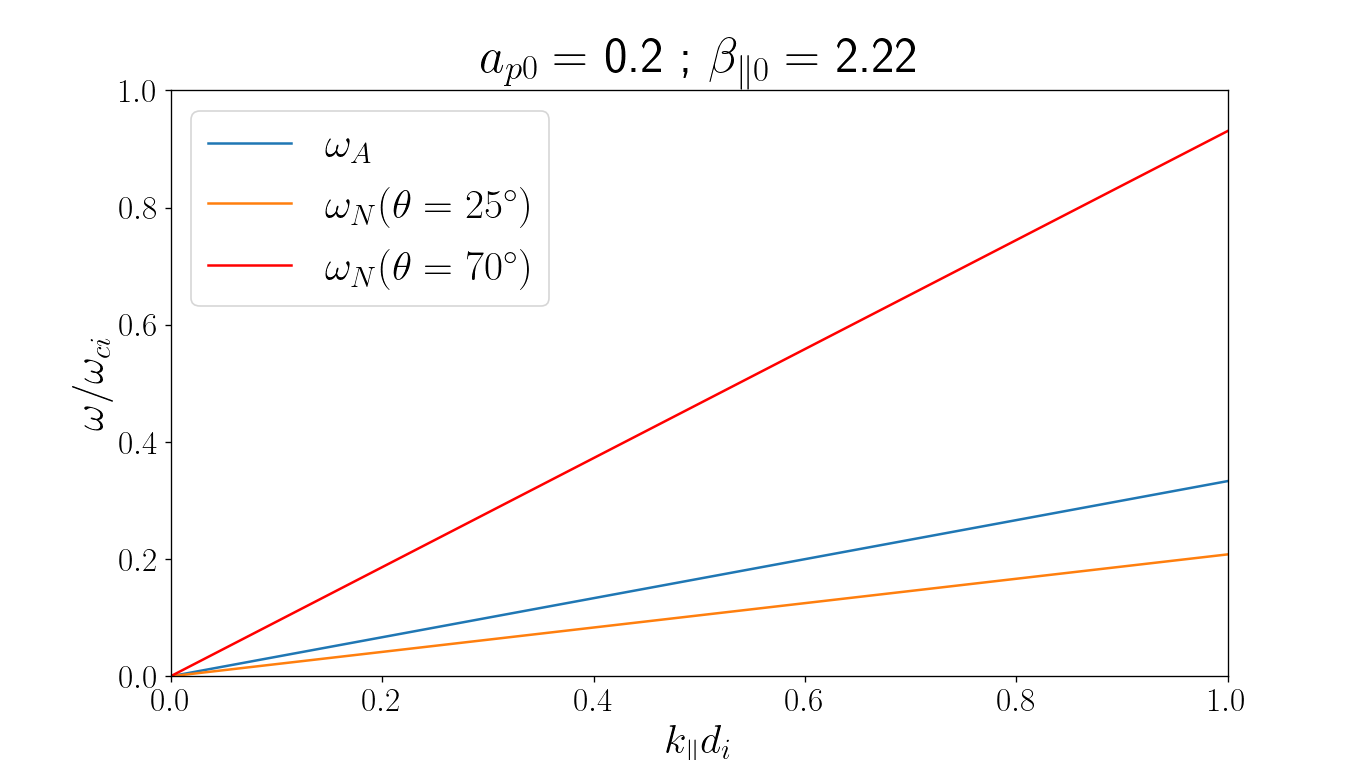
\includegraphics[width=0.8\linewidth,trim=2cm 0cm 3cm 1cm, clip=true]{./Part_2/images/lin_omega_k}
\caption{Mode d'Alfvén-firehose ($\omega_A$, bleu) et nouveau mode ($\omega_N $, orange pour $\theta = \ang{25}$ et rouge pour $\theta=\ang{70}$) normalisés par $\omega_{ci}$ la pulsation cyclotron des ions et représentés en fonction de $k_{\parallel}d_i$, avec $d_i = v_{A0}/ \omega_{ci}$, la longueur inertielle ionique. } 
\label{fig:lin_omega_k}
\end{figure}
On remarque que le nouveau mode peut être plus lent ou plus rapide que le mode d'Alfvén-firehose en fonction de $\theta$. Ce n'est pas montré ici, mais il peut aussi devenir instable quand le mode d'Alfvén-firehose est stable. Ils sont donc très différents. Ces observations, nous ont amené à faire une étude paramétrique en fonction de $\theta$ de la vitesse de phase et du taux de croissance/amortissement des instabilités. 

Au cours de cette étude, on a observé cinq comportements différents pour le nouveau mode suivant la valeur du couple  $\{\beta_{\parallel 0};a_{p0}\}$ . Ces comportements sont résumés sur la figure \ref{fig:lin_omega_theta} à travers cinq couples représentatifs. 
\begin{figure}[!ht]
 \centering
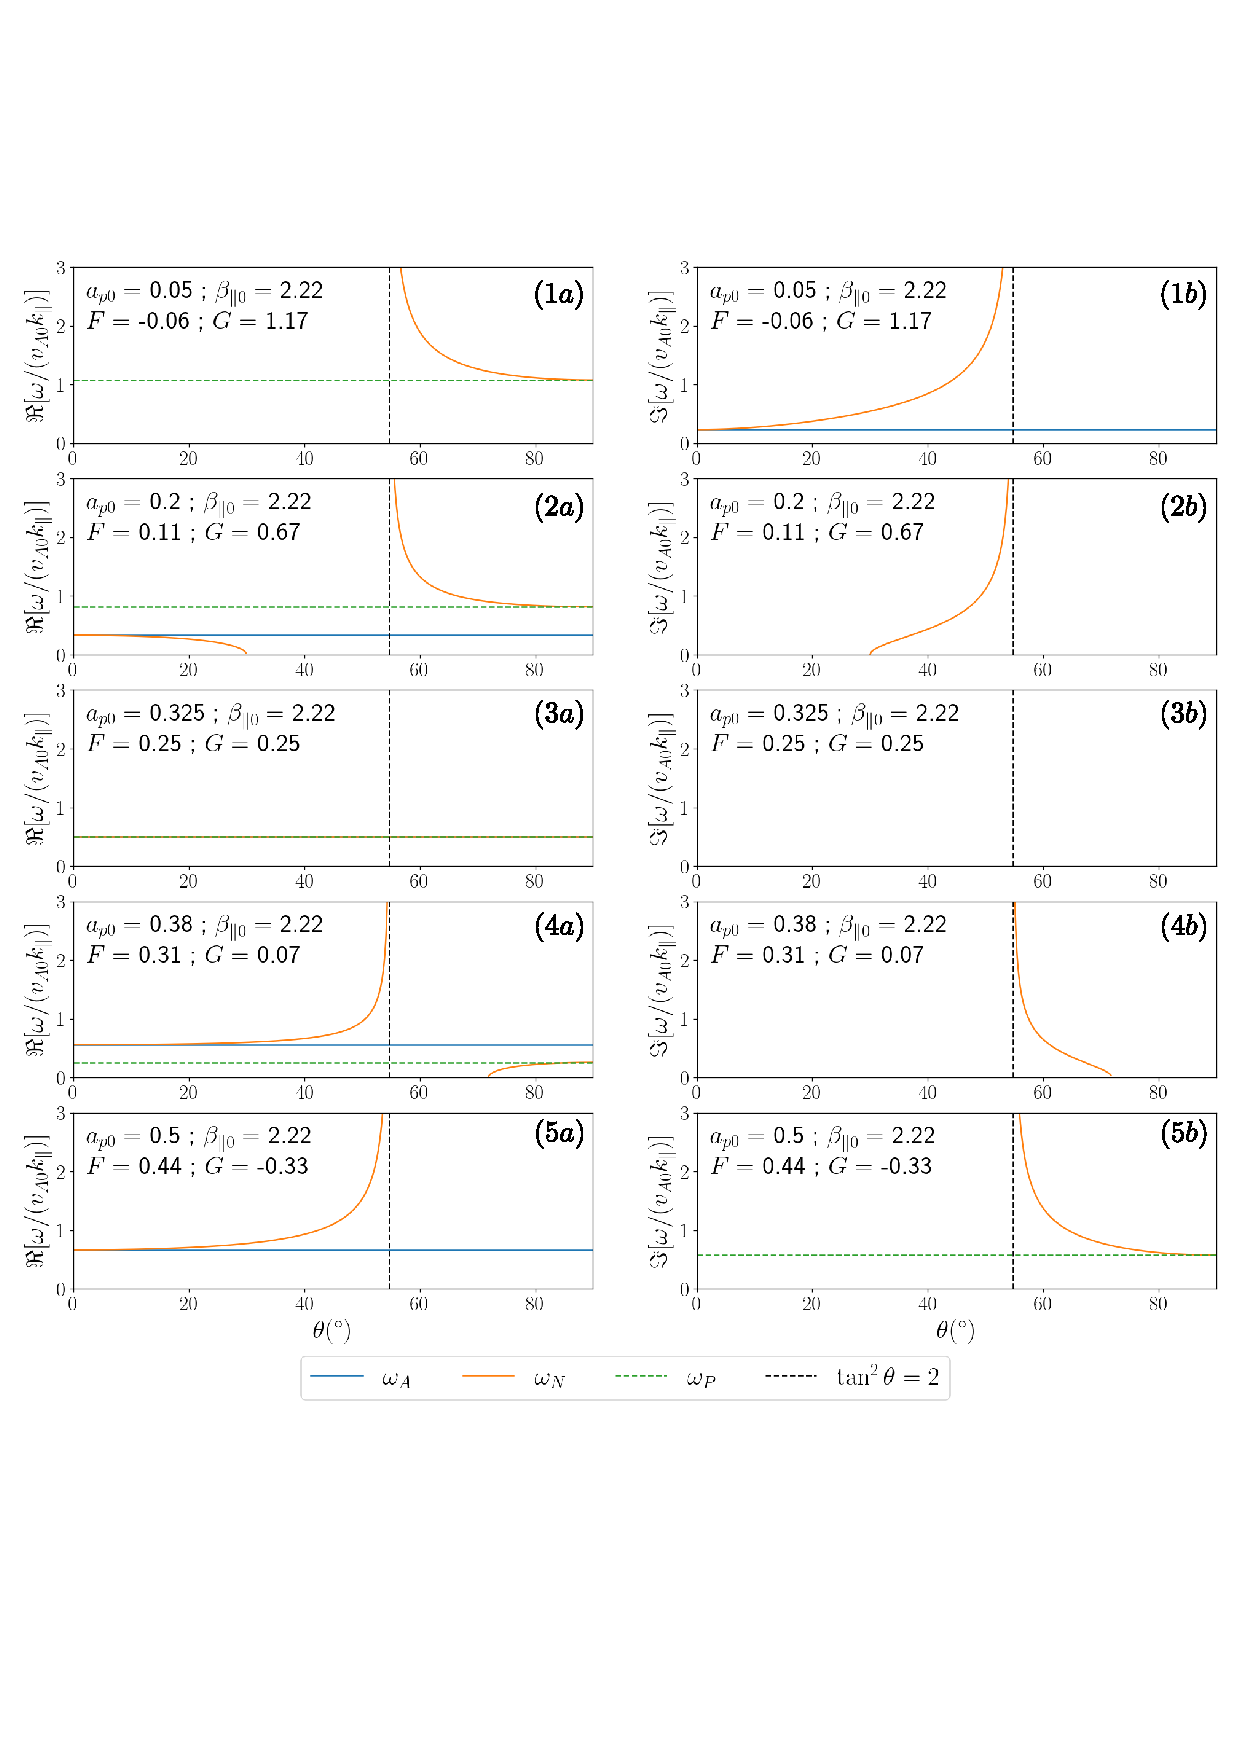
\includegraphics[width=\linewidth,trim=0.5cm 6cm 0cm 3cm, clip=true]{./Part_2/images/lin_omega_theta}
\caption{Vitesse de phase $\Re[\omega/(kv_{A0})]$ (colonne a) et taux de croissance des instabilités $\Im[\omega/(kv_{A0})]$ (colonne b) normalisées par $v_{A0}$ en fonction de l'angle $\theta$ pour le nouveau mode incompressible ($\omega_N$, orange) et pour le mode d'Alfvén ($\omega_A$, bleu). Des asymptotes sont tracées en lignes discontinues. En vert : mode asymptotique $\omega_P$. En noir : angle asymptotique $\theta_2$. Première ligne : couple (1) tel que $a_{p0} = 0.05$, $\beta_{\parallel 0} = 20/9 \Rightarrow$ instabilité firehose ($F<0$). Deuxième ligne : couple (2) tel que $a_{p0} = 0.2$, $\beta_{\parallel 0} = 20/9 $. Troisième ligne : couple (3) tel que $a_{p0} = 0.325$, $\beta_{\parallel 0} = 20/9 \Rightarrow$ seul cas stable pour tout $\theta$ ($F=G$). Quatrième ligne : couple (4) tel que $a_{p0} = 0.38$, $\beta_{\parallel 0} = 20/9  $. Cinquième ligne : couple (5) tel que $a_{p0} = 0.5$, $\beta_{\parallel 0} = 20/9  \Rightarrow$ instabilité pseudo-firehose perpendiculaire ($G<0$). Sauf graphique (3a) où tous les modes coincident, lorsque qu'un mode disparaît d'un graphique de la colonne a, il apparaît sur le graphique de la colonne b.}
\label{fig:lin_omega_theta}
\end{figure}
Sur l'ensemble de graphiques de la \figref{fig:lin_omega_theta} sont tracés en fonction de $\theta$, pour les cinq couples représentatifs et chaque mode, la partie réelle de $\omega$ normalisée par le mode d'Alfvén, $\Re[\omega/(k_{\parallel}v_{A0})]$ (colonne a) correspondant à sa vitesse de phase, ainsi que sa partie imaginaire ($\Im[\omega/(k_{\parallel}v_{A0})]$, colonne a), qui correspond au taux de croissance. $\omega$ étant ou réel ou purement imaginaire, ces graphiques sont complémentaires : si le mode est instable, il apparaîtra sur la colonne b, et s'il est stable sur la colonne a (à l'exception du graphique (3a) où les modes coîncident). Le caractère instable firehose du mode d'Alfvén (bleu) est ainsi retrouvé lorsque $F<0$ sur le graphique (1b). 

Le nouveau mode semble tendre asymptotiquement vers le mode d'Alfvén pour $\theta \sim \ang{0}$ et vers l'asymptote $\omega_P = \pm k_{\parallel}v_{A0} \sqrt{G}$ représentée par une ligne discontinue verte, pour $\theta \sim \ang{90}$. Une asymptote angulaire est aussi visible en un angle que l'on note $\theta_2$, on verra par la suite que cet angle est solution de $\tan^2 \theta = 2$. La stabilité du nouveau mode à une dépendance forte en $\theta$ : pour tout couple, il existe une gamme angulaire telle que le mode soit stable et, à l'exception du couple (3), une gamme telle que le mode est instable. 

On propose maintenant de démontrer les comportements identifiés pour le nouveau mode en fonction de $a_{p0}$ et $\beta_{\parallel 0}$. Au fil de cette analyse, on va construire le diagramme de la \figref{fig:lin_cases_update}. Les emplacements des différents couples présentés sur la \figref{fig:lin_omega_theta} sont indiqués par des croix rouges. 

\paragraph{Etude asymptotique angulaire : }Si $\theta \rightarrow \ang{0}$ ($k_{\parallel}\gg k_{\perp}$), alors $\frac{\omega^2_N}{v^2_{A0}k^2} \rightarrow F \cos^2 \theta$. La convergence vers le mode d'Alfvén-firehose du nouveau mode observée en $\theta \rightarrow \ang{0}$ sur la \figref{fig:lin_omega_theta} est ainsi vérifiée. Comme cette limite peut être stable ou instable en fonction du signe de $F$, on a représenté sur la \figref{fig:lin_cases_update}, la frontière $F=0$ en bleue et bleutée la zone où $F<0$. On retrouve dans ce comportement stable/instable l'instabilité firehose <<parallèle>> qui est présente par exemple pour le mode lent dans le cadre compressible. Le couple (1), tel que $F<0$, est un exemple instable : le nouveau mode et le mode d'Alfvén apparaîssent dans la colonne du taux de croissance (graphique (1b)). 

Si $\theta \rightarrow \ang{90}$ ($k_{\perp}\ll k_{\parallel} $), alors $\frac{\omega^2_N}{v^2_{A0}k^2} \rightarrow G \cos^2 \theta$. On retrouve l'asymptote $\omega_P$ et tracé en vert sur la \figref{fig:lin_omega_theta}. Il est instable si $G<0$. La comparaison de $G$ et $F$, qui ont la même structure à un facteur $3/2$ et un signe près, nous inspirant, on appellera cette instabilité <<instabilité pseudo-firehose perpendiculaire>>\footnote{Cette dénomination n'est proposée qu'à cause de la similarité des critères d'instabilités. Le comportement des quantités d'ordre 1 n'a pas été vérifié.}. Elle apparaît pour le couple (5) (graphique (5b)). Sur la \figref{fig:lin_cases_update}, on indique la frontière $G=0$ en vert et la zone où $G<0$ par une aire verte. 

{\bf Ainsi grâce à $F$ et $G$, on peut déduire qu'une instabilité pourra se développer dans le système pour tout couple $\{\beta_{\parallel 0};a_{p0}\}$ tel que $\frac{2}{3}>\frac{\beta_{\parallel 0}}{2}(1-a_{p0})$ (instabilité pseudo-firehose perpendiculaire, couple (5) et aire verte sur \figref{fig:lin_cases_update}) ou $\frac{\beta_{\parallel 0}}{2}(1-a_{p0})>1$ (instabilité firehose parallèle, couple (1) et aire bleue sur \figref{fig:lin_cases_update}).} Dans la zone intermédiaire (blanche sur la \figref{fig:lin_cases_update}), $G>0$ et $F>0$. 

\paragraph{Etude angulaire complète du nouveau mode : } Pour les angles $\theta$ plus obliques, le comportement de $\omega_N$ est plus difficile à établir, le signe de $\sin^2 \theta - 2 \cos^2 \theta$ venant compenser le signe de $G \sin^2 \theta - 2F \cos^2 \theta$. Une instabilité, entre l'instabilité firehose parallèle et l'instabilité pseudo-firehose perpendiculaire, pourra émerger. On la nommera <<instabilité pseudo-firehose oblique>>. Elle apparaît pour les couples (2) (graphique (2b)) et (4) (graphique (4b)). La condition d'instabilité est obtenue pour $F$ et $G$ tels que :  
\begin{eqnarray}
    (\tan^2 \theta - 2 )(G \tan^2 \theta - 2F ) &<& 0  .
\end{eqnarray}
$g(\theta) = (\tan^2 \theta - 2 )(G \tan^2 \theta - 2F )$ est une parabole présentant deux racines : 
\begin{itemize}
    \item $\tan^2 \theta = 2 $ en laquelle $\omega^2_N \rightarrow \infty$ (asymptote verticale indiquée en pointillés sur \figref{fig:lin_omega_theta}), on la note $\theta_2$,
    \item $\tan^2 \theta = 2\frac{F}{G}$ en laquelle $\omega^2_N \rightarrow 0$, on la note $\theta_{F/G}$.
\end{itemize}
La stabilité du nouveau mode dépendra donc de la position de $\theta$ par rapport à $\theta_2$ et $\theta_{F/G}$. 

Pour que le nouveau mode soit stable pour tout $\theta$, il faut $g(\theta)>0$ pour tout $\theta$. Cela n'est possible que si $F=G$, alors $g(\theta) = (\tan^2 \theta - 2 )^2 >0$. Dans ce cas, $\omega_N = \omega_A = \omega_P$. Sur la \figref{fig:lin_cases_update}, le critère $F=G$ est indiqué par la courbe noire et il est illustré par le couple (3) (graphiques (3a) et (3b)). {\bf Par conséquent, en fonction de $a_{p0}$ et $\beta_{\parallel 0}$, le nouveau mode sera stable pour tout $\theta$ si et seulement si $ \frac{\beta_{\parallel 0}}{2}(1-a_{p0}) = \frac{3}{4} $.}

$F=G$, $G=0$ et $F=0$ découpent le diagramme de la \figref{fig:lin_cases_update} en quatre zones que l'on va étudier séparément. 

Si $G<0$ (zone verte), alors $F>0$. Dans ce cas, $g(\theta) < 0$ si $\theta > \theta_2$. Cette situation est illustrée par le couple (5) (graphiques (5a) et (5b)), instable pour tout angle supérieur à $\theta_2$. On peut raccrocher à cette condition le cas $G=0$ puisque alors $F=1/3$, et la parabole sera négative si $\tan^2 \theta > 2$. Dans ces cas, on retrouve l'instabilité pseudo-firehose perpendiculaire découverte asymptotiquement si $\theta \rightarrow \ang{90}$. On peut maintenant compléter ses conditions d'existence qui deviennent : {\bf l'instabilité pseudo-firehose perpendiculaire peut se développer si $G<0$ pour tout angle $\theta > \theta_2$}.


Si $G>0$ et $F/G>1$ (zone blanche délimitée par les courbes verte et noire), $g(\theta) < 0$ si $2\frac{F}{G} > \tan^2 \theta > 2$. Cette situation est illustrée par le couple (4) (graphiques (4a) et (4b)). L'instabilité s'y développant est l'instabilité pseudo-firehose oblique. 


Si $G>0$ et $F/G<1$ (zone blanche délimitée par les courbes bleue et noire et zone bleue), $g(\theta) < 0$ si $2 > \tan^2 \theta > 2\frac{F}{G}$. {\bf Si $F<0$, l'instabilité firehose parallèle se développe pour tout angle  $\theta < \theta_2$. } Ce cas est illustré par le couple (1) (graphiques (1a) et (1b)). Si $F>0$, la situation est illustrée par le couple (2) (graphiques (2a) et (2b)). L'instabilité visible est encore une fois l'instabilité pseudo-firehose oblique. Sa condition d'apparition est donc : {\bf l'instabilité pseudo-firehose oblique peut se développer si $G>0$ et $F>0$ mais $G\neq F$, pour tout angle $\theta$ entre $\theta_2$ et $\theta_{F/G}$}. 

\begin{figure}[!ht]
 \centering
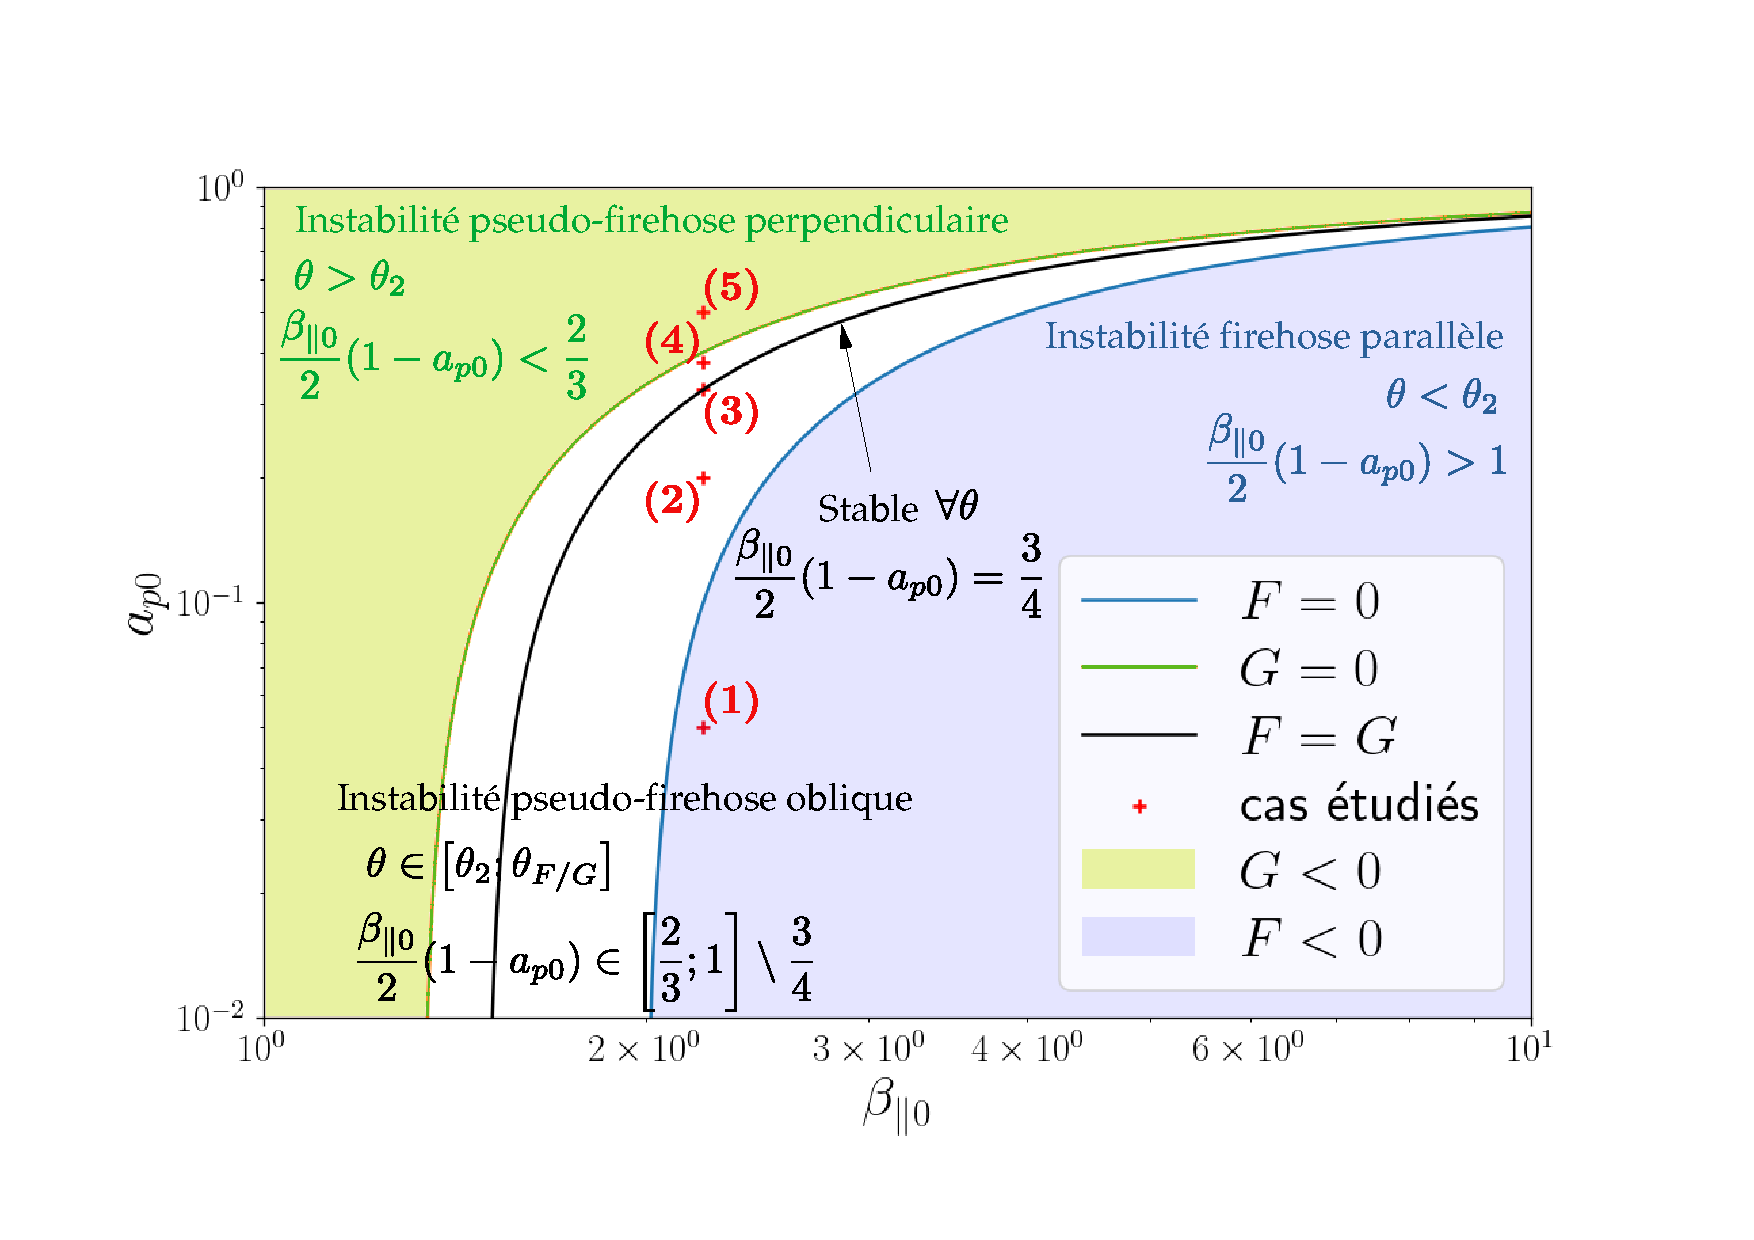
\includegraphics[width=1\linewidth,trim=2cm 1cm 3cm 2cm, clip=true]{./Part_2/images/diag_cas}
\caption{Diagramme $a_{p0}-\beta_{\parallel 0}$ résumant l'étude du nouveau mode. Croix rouges : couples $\{\beta_{\parallel 0};a_{p0}\}$ sélectionnés pour l'étude paramétrique de la \figref{fig:lin_omega_theta}. Frontière d'instabilités firehose $F=0$ (bleu) et zone instable ($F<0$, bleue) associée. Frontière d'instabilités pseudo-firehose perpendiculaire $G=0$ (verte) et zone instable ($G<0$, verte) associée. Ligne noire : ensemble des couples $\{\beta_{\parallel 0};a_{p0}\}$ stables pour tout angle $\theta$ paramétrisé par  $F=G$. Zone blanche : instabilité pseudo-firehose oblique. }
\label{fig:lin_cases_update}
\end{figure}


La zone de stabilité de ce nouveau mode en fonction des paramètres $\beta_{\parallel 0}$ et $a_{p0}$ est donc quasi-inexistante. Un résumé de l'ensemble des éléments de cette analyse est donnée sur la \figref{fig:lin_cases_update}. Sachant que la problématique principale de ce travail se place dans le cadre compressible, l'exploitation de ce modèle incompressible n'a pas été engagée mais il fera l'objet d'un nouveau papier en préparation [\cite{simon_article_2023}]. 


% \section{Limite incompressible du modèle \ac{CGL}}\label{sec-224}

% Dans le cas \ac{MHD} compressible avec pression isotrope, le mode pseudo-alfvénique apparaît comme une limite incompressible des modes compressibles magnétosonores. Similairement, on s'est demandé si l'on pouvait retrouver une trace du nouveau mode dans la limite incompressible du modèle \ac{CGL} linéaire. 

% Dans le cas linéaire, le modèle \ac{CGL} donne l'équation de dispersion \eqref{eq:lin_cpg_eqdis} que l'on va simplement noter $\overline{\boldsymbol{M}} \boldsymbol{v}_1 = 0$. Avec la contrainte incompressible $\nabla \cdot \boldsymbol{v}_1 = 0$, on peut écrire $\boldsymbol{v}_1$ sous la forme d'un potentiel vecteur $\boldsymbol{\Omega}$ : $\boldsymbol{v}_1 = \nabla \times \boldsymbol{\Omega} = \overline{\boldsymbol{N}}\boldsymbol{\Omega}$ avec $\overline{\boldsymbol{N}} = i \boldsymbol{k} \times \overline{\boldsymbol{I}} = i \begin{pmatrix} 0&-k_{\parallel}&0\\k_{\parallel}&0&-k_{\perp}\\ 0&k_{\perp}&0 \end{pmatrix} $. Le modèle \ac{CGL} linéaire surcontraint via l'incompressibilité s'exprime alors à travers l'équation de dispersion : $\overline{\boldsymbol{M}}  \overline{\boldsymbol{N}} \boldsymbol{\Omega}=0$ avec 
% \begin{equation}
%     \overline{\boldsymbol{M}} \overline{\boldsymbol{N}} = \begin{pmatrix}
% \label{eq:lin_cpginc_eqdis}  0&  -k_{\parallel}(\frac{\omega^2-\omega^2_A}{v^2_{A0}k^2_{\parallel}} -  (\frac{\beta_{\parallel 0}}{2} a_{p0} +1 ) \frac{k^2_{\perp}}{k^2_{\parallel}})  & 0  \\
%     k_{\parallel} \frac{\omega^2 - \omega^2_A}{v^2_{A0}k^2_{\parallel}}  & 0 & - k_{\perp}\frac{\omega^2-\omega^2_A}{v^2_{A0}k^2_{\parallel}}\\
%       0  &k_{\perp}(\frac{\omega^2 }{ v^2_{A0}k^2_{\parallel}} -   \frac{\beta_{\parallel 0}}{2}  (3-a_{p0})) &0 
%     \end{pmatrix} ,
% \end{equation}
% où $\omega^2_A = - v^2_{A0}k^2_{\parallel} ( \frac{\beta_{\parallel 0}}{2} (1-a_{p0})-1)$ correspond au mode d'Alfvén-firehose incompressible. On remarque que ce mode est solution si $\Omega_y = 0$, c'est-à-dire pour une polarisation de la vitesse orientée suivant $(0,1,0)$. 

% On a vu dans la section \ref{sec-222} que le nouveau mode est polarisé suivant $(\cos \theta,0,-\sin \theta)$.  Si l'on impose cette polarisation dans $\Omega$ on obtient $\Omega_y \neq 0$. Dans ce cas l'équation de dispersion peut alors s'écrire sous la forme du système :
% \begin{eqnarray}
%     \label{eq:lin_cglinc_1} k_{\parallel}(\omega^2-\omega^2_A - v^2_{A0}  (\frac{\beta_{\parallel 0}}{2} a_{p0} +1 ) k^2_{\perp}) &=& 0 ,\\
%      \label{eq:lin_cglinc_2} k_{\perp}(\omega^2  - v^2_{A0}   \frac{\beta_{\parallel 0}}{2}  (3-a_{p0}) k^2_{\parallel})&=& 0 ,\\
%      \label{eq:lin_cglinc_3} k_{\parallel}\Omega_x - k_{\perp}\Omega_z&=&0 .
% \end{eqnarray}
% On va étudier ce système en fonction de l'angle $\theta$ de propagation : 
% \begin{itemize}
%     \item $\theta = \ang{0} \Rightarrow k_{\perp} = 0$ et on suppose  $ k_{\parallel} \neq 0$, alors $\omega^2 =\omega^2_A$ et $\Omega_x =0$. On retrouve le mode firehose parallèle associé à un champ de vitesse sera polarisé suivant $(1,0,0)$.
%     \item $\theta = \ang{90} \Rightarrow k_{\parallel}  = 0$ et on suppose  $k_{\perp} \neq 0$, alors $\omega^2 =0$ et $\Omega_z =0$. On obtient un mode qui ne se propage pas et un champ de vitesse polarisé suivant $(0,0,1)$.
%     \item Si $ k_{\parallel} \neq 0$ et $k_{\perp} \neq 0$, alors $\omega^2  = v^2_{A0}   \frac{\beta_{\parallel 0}}{2}  (3-a_{p0})k^2_{\parallel}$ et $\theta$ doit vérifier $\tan^2 \theta  =\frac{2(\beta_{\parallel 0}(2-a_{p0})-1)}{\beta_{\parallel 0} a_{p0}+2}$.
% \end{itemize}
% Après quelques manipulations de $\omega^2  = v^2_{A0}   \frac{\beta_{\parallel 0}}{2}  (3-a_{p0})k^2_{\parallel}$ et de la condition $\tan^2 \theta  =\frac{2(\beta_{\parallel 0}(2-a_{p0})-1)}{\beta_{\parallel 0} a_{p0}+2}$, il est possible de faire ressortir la relation de dispersion du nouveau mode. 

% On remarque qu'appliquer la contrainte incompressible sur le modèle \ac{CGL} revient à chercher la limite telle que $p_{\parallel}$ ou $p_{\perp}$ respecte leur équation individuelle dans le modèle incompressible gyrotrope. En fait, la limite incompressible du modèle \ac{CGL} correspond à l'intersection des solutions des modèles incompressible gyrotrope défini avec la trace de la pression, incompressible gyrotrope défini avec l'équation sur $p_{\parallel}$ et incompressible gyrotrope défini avec l'équation sur $p_{\perp}$. Dans chacun de ces modèles, le mode d'Alfvén-firehose sera accompagné d'un nouveau mode dont l'expression dépend du choix de la fermeture sur la pression. Mais tous seront polarisé tel que $(\cos \theta,0,-\sin \theta)$ et peuvent être retrouvés dans le mode surcontraint du modèle \ac{CGL}. 

\newpage
\section{Synthèse : Limite incompressible et pistes d'étude}
\label{synt-22}

\fcolorbox{red}{white}{\begin{minipage}[c]{\linewidth}
\paragraph{Limite incompressible de la loi exacte avec pression tensorielle et cas gyrotrope :}
\begin{eqnarray}
    \label{eq:synth_turbinc_pgen} - 4(\varepsilon - \varepsilon_{PP98}) &=& -2 \left< \delta (\overline{\boldsymbol{P}} - p \overline{\boldsymbol{I}}):\delta (\nabla \boldsymbol{v}) \right> = -2 \left< \delta \overline{\boldsymbol{\Pi}} :\delta (\nabla \boldsymbol{v}) \right>,\\
\label{eq:synth_turbinc_pgyr} - 4(\varepsilon - \varepsilon_{PP98}) &=& -2 \left< \delta ((p_{\parallel} - p_{\perp})(\boldsymbol{b}\boldsymbol{b} -\frac{1}{3} \overline{\boldsymbol{I}})):\delta (\nabla \boldsymbol{v}) \right>.
\end{eqnarray}
$\Rightarrow$ Questionne l'existence d'un modèle incompressible gyrotrope. 


\paragraph{Modèle incompressible avec pression gyrotrope proposé compatible avec la loi exacte : }
\begin{eqnarray}
\label{eq:synth_incg_v} \partial_t  \boldsymbol{v} + \nabla \cdot (\boldsymbol{v}\boldsymbol{v} - \boldsymbol{v_A}\boldsymbol{v_A} + \frac{1}{\rho_0} \overline{\boldsymbol{P_*}})  &=& 0  ,\\
\label{eq:synth_incg_p} \partial_t p + \nabla \cdot (p \boldsymbol{v} ) + \frac{2}{3} \overline{\boldsymbol{\Pi}} : \nabla \boldsymbol{v}   &=& 0 ,  \\
\label{eq:synth_incg_b} \partial_t \boldsymbol{v_A} -  \nabla \cdot (\boldsymbol{v_A}\boldsymbol{v} - \boldsymbol{v}\boldsymbol{v_A}) &=& 0 ,\\
 \text{avec } \quad \overline{\boldsymbol{P_*}} = (p+p_m) \overline{\boldsymbol{I}} + \overline{\boldsymbol{\Pi}}, \quad p_m = \frac{\rho_0 | \boldsymbol{v_A}|^2}{2}, \quad p = \frac{1}{3} (2 p_{\perp} + p_{\parallel} ), &&  \nonumber\\ \overline{\boldsymbol{\Pi}} = (p_{\parallel} - p_{\perp})(\boldsymbol{b}\boldsymbol{b} - \frac{1}{3} \overline{\boldsymbol{I}}),  \quad \boldsymbol{b} = \frac{\boldsymbol{v_A}}{|\boldsymbol{v_A}|}, \quad \text{et} \quad \nabla \cdot \boldsymbol{v} &=&  0.  \nonumber
\end{eqnarray}

\paragraph{Etude linéaire du modèle proposé : }
\begin{itemize}
    \item Mode d'Alfvén incompressible polarisé suivant $(0,1,0)$ :
\begin{eqnarray}
\label{eq:synth_lininc_disp1}    
  \frac{\omega^2}{v^2_{A0}k^2_{\parallel}} + \frac{\beta_{\parallel 0}}{2}(1-a_{p0})-1  &=&0,\\
\text{Instabilité firehose : } \frac{\beta_{\parallel 0}}{2}(1-a_{p0})-1 &>&0 .
\end{eqnarray} 
    \item Nouveau mode polarisé suivant $(1,0,- \tan \theta)$ : (voir la \figref{fig:lin_cases_update})
\begin{eqnarray}
\label{eq:synth_lininc_disp2}    
  \frac{\omega^2}{v^2_{A0}k^2_{\parallel}} - \frac{2(\frac{\beta_{\parallel 0}}{2}(1-a_{p0})-1)\cos^2 \theta 
  +  ( 3\frac{\beta_{\parallel 0}}{2}(1-a_{p0}) - 2) \sin^2 \theta}{\sin^2 \theta-2\cos^2 \theta}  =0. && \\
\text{Critère d'instabilité pseudo-firehose : }  \frac{\beta_{\parallel 0}}{2}(1-a_{p0}) \neq \frac{3}{4}. && 
\end{eqnarray} 
\end{itemize}

% \paragraph{\\Limite incompressible du modèle \ac{CGL} :}
% \begin{itemize}
%     \item Survie du mode d'Alfvén-firehose $\Rightarrow$ Solution non-linéaire, pendant gyrotrope du mode d'Alfvén non linéaire ?
%     \item Apparition d'un mode surcontraint correspondant au nouveau mode incompressible.
% \end{itemize}

Les résultats obtenus ici à propos du nouveau modèle semble prometteur et feront l'objet d'une publication future. 
\end{minipage}}


\chapitre{Relaxer l'approximation MHD et aller vers le bi-fluide}{ch-23}
\chapter{Relaxer l'approximation \ac{MHD} et aller vers le bi-fluide}
\renewcommand\partie{\Partie\ Chapitre \thechapter}
\label{ch-23}
\bigskip
\minitoc  

Dans les chapitres précédents, l'équation d'induction \eqref{eq:model_cpg_b} était celle de l'approximation \ac{MHD}. Dans ce chapitre, nous allons relaxer les hypothèses sur cette équation en prenant d'abord en compte le terme de \acs{Hall} (section \ref{sec-231}). Dans la section \ref{sec-233}, nous dériverons une correction à la loi exacte associée à chaque niveau d'approximation de la loi d'Ohm en partant du modèle bi-fluide. Enfin dans la section \ref{sec-232}, nous nous intéresserons au modèle gyrotrope utilisé dans les simulations étudiées dans la Partie \ref{part_3} : un modèle \acs{LFCGLHPe} (avec la fermeture \ac{LF} gyrotrope telle que $\overline{\overline{\boldsymbol{q}}} \neq 0$) prenant en compte la pression électronique dans la loi d'Ohm avec différentes fermetures (isotherme et gyrotrope). 

\section{La \acs{MHDH}}
\label{sec-231}

Comme on l'a vu dans le Chapitre \ref{ch-02}, le terme de \acs{Hall} doit être pris en compte dans l'équation d'induction si l'on regarde des échelles proches de la longueur inertielle des ions, ou des fréquences proches de la fréquence cyclotron des ions. Par conséquent, la loi exacte obtenue avec une loi d'Ohm \ac{MHD} perdra en validité près de ces échelles. Afin de tirer la description de la cascade dans ce domaine ionique, on doit donc calculer une correction à partir du terme de \acs{Hall}. Diverses formulations existent pour cette contribution dans le cas des modèles dépendant d'une pression isotrope mais que devient-elle dans le cadre d'une fermeture avec pression tensorielle ? 

En prenant en compte le terme de \acs{Hall}, l'équation d'induction devient : 
\begin{equation}
\label{eq:model_hall1} \partial_t \boldsymbol{v_A}  =   \nabla \cdot \left(\boldsymbol{v_A}\boldsymbol{u} - \boldsymbol{u}\boldsymbol{v_A}\right) -  \boldsymbol{u}  \nabla \cdot \boldsymbol{v_A} +  \frac{\boldsymbol{v_A}}{2}  \nabla \cdot \boldsymbol{u} - \frac{\lambda_i}{ \sqrt{\rho} } \nabla \times \left(\frac{\boldsymbol{j}}{\sqrt{\rho}}  \times \boldsymbol{v_A}\right) ,
\end{equation}
avec $\lambda_i = m_i/|q_e|$, constante analysée dans le chapitre \ref{ch-02} de l'Introduction,  $\boldsymbol{j} = \frac{1}{\sqrt{\mu_0}} \nabla \times \left(\sqrt{\rho}\boldsymbol{v_A}\right)$, la densité de courant et $\mu_0$ la perméabilité du vide. 

Puisque $\sqrt{\rho} \boldsymbol{v_A} \cdot \nabla \times \left(\frac{\boldsymbol{j}}{\sqrt{\rho}}  \times \boldsymbol{v_A}\right) = \nabla \cdot \left(\left(\boldsymbol{j}  \times \boldsymbol{v_A}\right)\times \boldsymbol{v_A} \right)$, l'équation d'énergie magnétique \eqref{eq:model_cpi_m} devient :
\begin{equation}
  \label{eq:model_cpgh_m}   \partial_t E_m  +\nabla   \cdot  \left(E_m\boldsymbol{v}+ \lambda_i \left(\boldsymbol{j}  \times \boldsymbol{v_A}\right)\times \boldsymbol{v_A} \right)  = \rho  \boldsymbol{v_A}\boldsymbol{v_A}  : \nabla \boldsymbol{v}- p_m  \nabla \cdot \boldsymbol{v} .
\end{equation}
Cette correction n'ajoute qu'un terme de type flux au bilan énergétique et n'impactera pas l'équation d'énergie interne. De plus, le terme de \acs{Hall} ne dépend pas du tenseur de pression. Par conséquent, elle n'influera pas littéralement sur les contributions du tenseur de pression et de l'énergie interne dans la loi exacte. Il faudra tout de même faire attention à ne pas utiliser les formes conservatives des pressions parallèle et perpendiculaire \acs{CGL} \eqref{eq:model_cpg_biadiab} qui ne sont valables que dans le cas \ac{MHD}, l'équation d'induction \ac{MHD} étant utilisée pour les obtenir.

En notant génériquement $\varepsilon_{mhd}$ le taux de cascade compressible obtenu avec un modèle dans lequel le terme de \acs{Hall} est négligé et $\varepsilon_{hall}$ la correction \acs{Hall}, le nouveau taux de cascade sera $\varepsilon = \varepsilon_{mhd} + \varepsilon_{hall}$ avec  :
%\begin{eqnarray}
\begin{equation}
\label{eq:corr_hall} \boxed{
\begin{array}{lcl}
    -4\varepsilon_{hall} &=& \lambda_i\nabla_{\boldsymbol{\ell}} \cdot \left< \left(\boldsymbol{j}  \times \boldsymbol{v_A}+ \boldsymbol{j'}  \times \boldsymbol{v'_A}\right)\times \delta \boldsymbol{v_A} - \delta \left(\frac{\boldsymbol{j}}{\rho}  \times \boldsymbol{v_A}\right)\times \left(\rho \boldsymbol{v_A}+ \rho' \boldsymbol{v'_A}\right)\right> \\
    &+& \frac{\lambda_i}{2} \left< \left(\rho' \boldsymbol{v'_A} \cdot \delta \boldsymbol{v_A}- \delta \left(\rho \boldsymbol{v_A}\right) \cdot \boldsymbol{v'_A} \right)\nabla \cdot \left(\frac{\boldsymbol{j}}{\rho}\right) - \left(\rho \boldsymbol{v_A} \cdot \delta \boldsymbol{v_A}- \delta \left(\rho \boldsymbol{v_A}\right) \cdot \boldsymbol{v_A} \right) \nabla' \cdot \left(\frac{\boldsymbol{j'}}{\rho'}\right)\right> \\%\nonumber 
    &-& \lambda_i \left< \left(\rho' \boldsymbol{v'_A} \cdot \delta \left(\frac{\boldsymbol{j}}{\rho}\right)- \boldsymbol{v'_A} \cdot \delta \boldsymbol{j}  \right)\nabla \cdot \boldsymbol{v_A} - \left(\rho \boldsymbol{v_A} \cdot \delta \left(\frac{\boldsymbol{j}}{\rho}\right)- \boldsymbol{v_A} \cdot \delta \boldsymbol{j}  \right)\nabla' \cdot \boldsymbol{v'_A}\right> .
   \end{array}}
\end{equation} 
%\end{eqnarray}
Ce résultat est une adaptation à nos notations du résultat obtenu par \cite{andres_exact_2018} qui utilise la même fonction de corrélations de l'énergie magnétique, $\mathcal{R}_{m} = \frac{1}{4}\left<\left(\rho'+\rho\right)\boldsymbol{v'_A} \cdot \boldsymbol{v_A}\right>$, que nous.

Dans le cas incompressible avec pression isotrope, diverses formes de $\varepsilon_{hall}$ existent et ont été comparées par \cite{ferrand_exact_2019}. 
On retiendra la forme qu'ils ont dérivée et qui peut être retrouvée en prenant la limite incompressible de la correction \eqref{eq:corr_hall} :
\begin{equation}
\label{eq:corr_hallinc} \boxed{
\begin{array}{lcl}
    -4 \varepsilon_{hall} &{}_{\overrightarrow{\rho = \rho_0}}&  -\frac{\lambda_i}{2} \nabla_{\boldsymbol{\ell}} \cdot \left<\delta \boldsymbol{v_A} \cdot \delta \boldsymbol{v_A}\delta \boldsymbol{j} - 2 \delta \boldsymbol{v_A} \cdot \delta \boldsymbol{j} \delta \boldsymbol{v_A}\right> . %\nonumber \\ 
   \end{array}}
\end{equation} 
Similairement à la correction compressible, cette correction est applicable à notre loi incompressible avec pression gyrotrope. 

Linéairement, le terme de \acs{Hall} va adapter les modes \ac{MHD} et \acs{CGL} afin d'y faire apparaître des corrections proches de la fréquence cyclotron ionique $\omega_{ci} = \frac{B_0}{\lambda_i}$. Des modes whistler (sifflants) et cyclotron ionique vont émerger. Pour plus de détails, se référer à la dérivation effectuée par \cite{hunana_introductory_2019}. On notera que plus l'angle de propagation sera oblique par rapport à $\boldsymbol{b_0}$ et plus la correction \acs{Hall} à la relation de dispersion sera affaiblie. En terme d'instabilité, l'instabilité firehose sera quelque peu stabilisée. En effet, le critère d'instabilité devient $\frac{\beta_{\parallel 0}}{2}(1- a_{p0} ) > 1+\frac{k_{\parallel}^2 v^2_{A0}}{4\omega^2_{ci}}$. Par conséquent, la zone de stabilité du cadran $a_{p0}<1$ dans le diagramme $a_{p0}-\beta_{\parallel0}$ (\figref{fig:diag_cgl}) sera élargie : en $a_{p0}=0$, le critère rejoindra $\beta_{\parallel 0} = 2+\frac{k_{\parallel}^2 v^2_{A0}}{2\omega^2_{ci}}$ qui est supérieur au $\beta_{\parallel 0} = 2$ obtenu dans le cas \acs{CGL}. Le critère miroir ne sera quant à lui pas modifié. 

\section{Le modèle bi-fluide}
\label{sec-233}

Par curiosité, on s'est demandé à quoi ressemblerait la loi exacte si l'on prenait en compte l'ensemble de la loi d'Ohm généralisée \eqref{eq:ohm} dans l'équation d'induction. Au lieu d'attaquer ce problème en relaxant petit à petit les approximations appliquées sur la loi d'Ohm, j'ai choisi de partir du modèle bi-fluide puis d'y prendre en compte la quasi-neutralité et de l'exprimer en fonction des grandeurs mono-fluide et enfin d'y injecter la loi d'Ohm généralisée. Il est ensuite possible de faire tendre la loi exacte obtenue vers différents régimes similairement au travail effectué par \cite{banerjee_scale--scale_2020}. Contrairement à \cite{banerjee_scale--scale_2020} proposant une loi dérivée avec un modèle bi-fluide fermé polytropiquement et similairement à la dérivation effectuée dans le Chapitre \ref{ch-21}, on considèrera des pressions tensorielles et les équations d'énergie interne associée à chaque espèce en négligeant les flux de chaleur. Pour alléger un peu le calcul, on ne fait pas apparaître non plus les termes de forçage et dissipation.

La fonction de corrélation pour l'énergie électromagnétique sera choisie au plus près de celle utilisée jusqu'à présent c'est-à-dire $\left<\rho \boldsymbol{v_A}\cdot \boldsymbol{v'_A}\right>$.

Les équations bi-fluides utilisées
%non relativiste\footnote{L'hypothèse non-relativiste nous permet de négliger $q_r n_r \boldsymbol{E}$ devant $q_r n_r \boldsymbol{v_r} \times \boldsymbol{B}$  dans \eqref{eq:model_bi_v} (on l'y indique entre parenthèse car on en aura besoin dans la loi d'Ohm généralisée) et $\varepsilon_0 \mu_0 \partial_t \boldsymbol{E}$ devant $\nabla \times \boldsymbol{B}$ dans \eqref{eq:model_bi_EB3}.} utilisée avec $r = i,e$ 
sont : 
\begin{eqnarray}
  \label{eq:model_bi_r} \partial_t \rho_{\alpha} + \nabla \cdot \left(\rho_{\alpha} \boldsymbol{v_{\alpha}}\right) &=& 0 ,\\
  \label{eq:model_bi_v} \partial_t \left(\rho_{\alpha} \boldsymbol{v_{\alpha}}\right) + \nabla \cdot \left(\rho_{\alpha} \boldsymbol{v_{\alpha}}\boldsymbol{v_{\alpha}} + \overline{\boldsymbol{P_{\alpha}}}\right) - Q_{\alpha} \boldsymbol{E} - \boldsymbol{j_{\alpha}} \times \boldsymbol{B} &=& 0 ,\\
  \label{eq:model_bi_u} \partial_t  u_{\alpha} + \boldsymbol{v_{\alpha}} \cdot \nabla u_{\alpha}   + \frac{1}{\rho_{\alpha}} \overline{\boldsymbol{P_{\alpha}}} : \nabla \boldsymbol{v_{\alpha}}   &=& 0 ,\\
\label{eq:model_bi_EB1} \nabla \cdot \boldsymbol{E} =  \frac{Q}{\varepsilon_0} \qquad \nabla \times \boldsymbol{B} = \mu_0  \boldsymbol{j} + \mu_0 \varepsilon_0 \partial_t \boldsymbol{E} \qquad \nabla \cdot \boldsymbol{B} &=& 0 , \\
\label{eq:model_bi_EB4}\partial_t \boldsymbol{B} + \nabla \times \boldsymbol{E}   &=&  0 ,
\end{eqnarray}
avec $Q = \sum_{\alpha} Q_{\alpha} =  \sum_{\alpha} q_{\alpha} n_{\alpha}$, $\boldsymbol{j} = \sum_{\alpha} \boldsymbol{j_{\alpha}} = \sum_{\alpha} q_{\alpha} n_{\alpha} \boldsymbol{v_{\alpha}}  $. 

Ces équations contiennent beaucoup de quantités constantes : $m_{\alpha}$ dans $\rho_{\alpha}$, $q_{\alpha}$ pour chaque espèce, $ \mu_0$, $\varepsilon_0$. Afin de réduire ce nombre de constantes qui viendront alourdir les calculs et de faire ressortir des constantes caractéristiques du plasma, nous allons normaliser les équations\footnote{Cela n'a pas été entreprit dans les modèles mono-fluides utilisés précédemment, parce qu'en \acs{MHD} et \ac{MHDH}, les seules échelles apparaissant sont celles des ions (puisque $m_e \ll m_i$).}. 
Ces constantes caractéristiques sont le rapport de masse $\mu = \frac{m_e}{m_i+m_e} \simeq \frac{m_e}{m_i}$ puisque $m_e \ll m_i$, qui permet d'accéder facilement aux régimes \ac{MHD} ($\mu \rightarrow 0$) ou \ac{MHD} électronique (\acs{EMHD}, $\mu \rightarrow 1$) et une longueur inertielle sans dimension $\lambda_i = \frac{\sqrt{m_i+m_e}}{L_0 \sqrt{\mu_0 n_0 e^2}} \simeq \frac{\sqrt{m_i}}{L_0 \sqrt{\mu_0 n_0 e^2}}$ que l'on note $\lambda_i$ pour faciliter les comparaisons avec les résultats dimensionnés. Les vitesses seront normalisées par la vitesse de la lumière dans le vide $c$, et l'on note les quantités de références :
\begin{itemize}
    \item Longueur : $L_0$,
    \item Temps : $t_0 = \frac{L_0}{c}$,
    \item Vitesse : $V_0 = c$,
    \item Densité de particule : $n_0$,
    \item Champ magnétique : $B_0 = c \sqrt{\mu_0 n_0 (m_i+m_e)}$,
    \item Champ électrique : $E_0 = c B_0$,
    \item Pression : $P_0 = (m_i+m_e)n_0 c^2$.
\end{itemize}
On pourrait noter les quantités sans dimension avec un << $\tilde{}$ >>, par exemple $\tilde{\boldsymbol{v_i}} = \boldsymbol{v_i}/V_0$, etc. Cependant, dans la suite de cette section, on ne fera pas apparaître les << $\tilde{}$ >> afin d'alléger les notations.

Le système sans dimension s'écrit donc :
\begin{eqnarray}
  \label{eq:model_adbi_ri} \partial_t n_i + \nabla \cdot \left(n_i \boldsymbol{v_i}\right) &=& 0, \\
  \label{eq:model_adbi_re} \partial_t n_e + \nabla \cdot \left(n_e \boldsymbol{v_e}\right) &=& 0, \\
  \label{eq:model_adbi_vi} \partial_t  \boldsymbol{v_i} +\boldsymbol{v_i} \cdot \nabla \boldsymbol{v_i} + \frac{1}{(1-\mu) n_i} \nabla \cdot \overline{\boldsymbol{P_i}} - \frac{1}{(1-\mu)\lambda_i} \boldsymbol{E} - \frac{1}{(1-\mu)\lambda_i}  \boldsymbol{v_i} \times \boldsymbol{B} &=& 0 ,\\
  \label{eq:model_adbi_ve}  \partial_t  \boldsymbol{v_e} +\boldsymbol{v_e} \cdot \nabla \boldsymbol{v_e} + \frac{1}{\mu n_e} \nabla \cdot \overline{\boldsymbol{P_e}} + \frac{1}{\mu \lambda_i}  \boldsymbol{E} + \frac{1}{\mu \lambda_i} \boldsymbol{v_e} \times \boldsymbol{B} &=& 0 ,\\
  \label{eq:model_adbi_ui} \partial_t  u_i + \boldsymbol{v_i} \cdot \nabla u_i   + \frac{1}{(1-\mu)n_i} \overline{\boldsymbol{P_i}} : \nabla \boldsymbol{v_i}   &=& 0 ,\\
\label{eq:model_adbi_ue} \partial_t  u_e + \boldsymbol{v_e} \cdot \nabla u_e   + \frac{1}{\mu n_e} \overline{\boldsymbol{P_e}} : \nabla \boldsymbol{v_e}   &=& 0 ,\\
\label{eq:model_adbi_EB1} \nabla \cdot \boldsymbol{E} =   \frac{1}{\lambda_i} (n_i -n_e) ,\qquad \nabla \times \boldsymbol{B} = \frac{1}{\lambda_i} (n_i \boldsymbol{v_i} - n_e \boldsymbol{v_e}) +  \partial_t \boldsymbol{E} ,
\qquad \nabla \cdot \boldsymbol{B} &=& 0  ,  \\
\label{eq:model_adbi_EB4}  \partial_t \boldsymbol{B}  + \nabla \times \boldsymbol{E}  &=& 0.
% \label{eq:model_adbi_r}  \partial_t \tilde{n_r} + \tilde{\nabla} \cdot (\tilde{n_r} \tilde{\boldsymbol{v_r}}) &=& 0\\
% \label{eq:model_adbi_vi}   \tilde{\partial_t}  \tilde{\boldsymbol{v_i}} +  \tilde{\boldsymbol{v_i}} \cdot \tilde{\nabla} \tilde{\boldsymbol{v_i}} + \frac{1}{(1-\mu) \tilde{n_i}} \tilde{\nabla} \cdot \tilde{\overline{\boldsymbol{P_i}}}  &=&  \frac{\lambda_i}{(1-\mu)} \tilde{\boldsymbol{v_i}} \times \tilde{\boldsymbol{B}} (+\frac{\lambda_i}{(1-\mu)} \tilde{\boldsymbol{E}}) \\
% \label{eq:model_adbi_ve}  \tilde{\partial_t}  \tilde{\boldsymbol{v_e}} +  \tilde{\boldsymbol{v_e}} \cdot  \tilde{\nabla} \tilde{\boldsymbol{v_e}} + \frac{1}{\mu \tilde{n_e}} \tilde{\nabla} \cdot \tilde{\overline{\boldsymbol{P_e}}}  &=&  -\frac{\lambda_i}{\mu} \tilde{\boldsymbol{v_e}} \times \tilde{\boldsymbol{B}}  (-\frac{\lambda_i}{\mu} \tilde{\boldsymbol{E}}) \\
% \label{eq:model_adbi_ui}    \tilde{\partial_t}  \tilde{u_i} +  \tilde{\boldsymbol{v_i}} \cdot \tilde{\nabla}  \tilde{u_i} +  \frac{1}{(1-\mu) \tilde{n_i}}  \tilde{\overline{\boldsymbol{P_i}}} : \tilde{\nabla} \tilde{\boldsymbol{v_i}}   &=& 0 \\
% \label{eq:model_adbi_ue}   \tilde{\partial_t}  \tilde{u_e} + \tilde{\boldsymbol{v_e}}  \cdot \tilde{\nabla}  \tilde{u_e} +  \frac{1}{\mu \tilde{n_e}}\tilde{\overline{\boldsymbol{P_e}}} : \tilde{\nabla} \tilde{\boldsymbol{v_e}}   &=& 0 \\
% \label{eq:model_adbi_EB1} \tilde{\nabla} \cdot \tilde{\boldsymbol{E}} &=& \lambda_i  (\tilde{n_i}-\tilde{n_e}) \\
% \label{eq:model_adbi_EB2} \tilde{\nabla} \cdot \tilde{\boldsymbol{B}} &=& 0  \\
% \label{eq:model_adbi_EB3}  \tilde{\nabla} \times \tilde{\boldsymbol{B}} &=& \lambda_i (\tilde{n_i} \tilde{\boldsymbol{v_i}} - \tilde{n_e} \tilde{\boldsymbol{v_e}}) \\
% \label{eq:model_adbi_EB4}  \tilde{\nabla} \times \tilde{\boldsymbol{E}}  &=&  - \tilde{\partial_t} \tilde{\boldsymbol{B}} 
\end{eqnarray}
Les grandeurs mono-fluides seront alors définies telles que $\rho  = (1-\mu) n_i + \mu n_e $ pour la densité, $\boldsymbol{v} = \frac{(1-\mu) n_i \boldsymbol{v_i} + \mu n_e \boldsymbol{v_e}}{(1-\mu) n_i + \mu n_e}$ pour la vitesse, $\boldsymbol{j} =  \frac{1}{\lambda_i} (n_i \boldsymbol{v_i} - n_e \boldsymbol{v_e})$ pour la densité de courant. Elles permettront de compacter un peu les équations. 
En combinant les équations \eqref{eq:model_adbi_ri}, \eqref{eq:model_adbi_re}, \eqref{eq:model_adbi_vi} et \eqref{eq:model_adbi_ve}, on obtient l'évolution de $\boldsymbol{j}$ qui sera nécessaire pour remplacer $\boldsymbol{E}$ dans \eqref{eq:model_adbi_EB4} : 
\begin{eqnarray}
\label{eq:model_adbi_j} \boldsymbol{E} &=& -  \frac{\rho}{\mu n_i + (1-\mu) n_e} \boldsymbol{v}  \times \boldsymbol{B} 
-   \frac{\lambda_i(2\mu-1)}{\mu n_i + (1-\mu) n_e}  \boldsymbol{j} \times \boldsymbol{B}
+  \lambda_i \frac{\mu \nabla \cdot \overline{\boldsymbol{P_i}} - (1-\mu) \nabla \cdot \overline{\boldsymbol{P_e}}}{\mu n_i + (1-\mu) n_e} \nonumber\\
&&+\frac{\lambda_i^2 \mu (1-\mu)}{\mu n_i + (1-\mu) n_e} \left[\partial_t \boldsymbol{j} + \nabla \cdot (
\frac{\rho \rho}{n_i n_e}  \boldsymbol{v}  \boldsymbol{j}  
+\frac{\rho \rho}{n_i n_e}  \boldsymbol{j}  \boldsymbol{v} 
+\frac{ \lambda_i(2\mu -1 )n_i}{n_i n_e}\boldsymbol{j} \boldsymbol{j} ) \right] \nonumber \\
&&+\frac{\lambda_i \mu (1-\mu)}{\mu n_i + (1-\mu) n_e} \nabla \cdot (
\frac{n_e - n_i}{n_i n_e} (\rho^2 \boldsymbol{v} \boldsymbol{v} + \mu^2\lambda_i^2 \boldsymbol{j} \boldsymbol{j})  ).
\end{eqnarray}
Contrairement à la loi d'Ohm détaillée dans le Chapitre \ref{ch-02}, on n'y suppose ni la quasi-neutralité ($n_i = n_e = \rho$) qui vient annuler la dernière ligne, ni $\mu \rightarrow 0$. À partir d'ici, on supposera l'hypothèse non-relativiste, qui permet de négliger les termes dépendant de $\boldsymbol{E}$ devant ceux dépendant de $\boldsymbol{B}$ dans \eqref{eq:model_adbi_vi} et \eqref{eq:model_adbi_ve} et \eqref{eq:model_adbi_EB1}. Comme on a besoin de l'équation d'induction, on doit garder le champ électrique dans l'équation \eqref{eq:model_adbi_j} et  \eqref{eq:model_adbi_EB4}. L'hypothèse non relativiste sera donc appliquée sur \eqref{eq:model_adbi_j} en fonction de l'usage.

On définit aussi la vitesse d'Alfvén telle que $\boldsymbol{v_A} = \frac{\boldsymbol{B}}{\sqrt{(1-\mu) n_i + \mu n_e}}$. L'énergie totale non relativiste de ce système peut ainsi être séparée entre une énergie totale ionique et une électronique : 
\begin{equation*}
E_{tot} = E_{toti} + E_{tote} =  \frac{1}{2} (1-\mu) n_i (|\boldsymbol{v_i}|^2 + |\boldsymbol{v_A}|^2 + 2 u_i) + \frac{1}{2} \mu n_e (|\boldsymbol{v_e}|^2 + |\boldsymbol{v_A}|^2 + 2 u_e).
\end{equation*}

L'équation d'induction \eqref{eq:model_adbi_EB4} s'écrit en fonction de la vitesse d'Alfvén : 
\begin{eqnarray}
\label{eq:model_adbi_B}  \partial_t \boldsymbol{v_A} &=& - \frac{\nabla \times  \boldsymbol{E}}{\sqrt{(1-\mu) n_i + \mu n_e}} + \frac{\boldsymbol{v_{A}}}{2}\frac{\nabla \cdot ((1-\mu) n_i \boldsymbol{v_i}+\mu n_e \boldsymbol{v_e})}{(1-\mu) n_i + \mu n_e}  .
\end{eqnarray}


En appliquant la méthode résumée dans la section \ref{ch-11} sur les fonctions de corrélations d'énergie totale ionique, $\mathcal{R}_{tot i} = \frac{1-\mu}{4} \left<  (n'_i + n_i) (\boldsymbol{v'_i} \cdot \boldsymbol{v_i} + \boldsymbol{v'_A} \cdot \boldsymbol{v_A}) + 2 n'_i u_i + 2 n_i u'_i \right>$, et électronique,  $ \mathcal{R}_{tot e} = \frac{\mu}{4} \left<  (n'_e + n_e) (\boldsymbol{v'_e} \cdot \boldsymbol{v_e} + \boldsymbol{v'_A} \cdot \boldsymbol{v_A}) + 2 n'_e u_e + 2 n_e u'_e \right> $ puis en supposant les hypothèses de stationnarité statistique et de séparation d'échelles de Kolmogorov, on obtient les lois exactes pour les taux de cascade, $\varepsilon_i$ et $\varepsilon_e$, associés à chaque fluide et exprimés dans la zone inertielle  :
\begin{eqnarray}
%\begin{equation} \boxed{\begin{array}{lcl}
  \label{eq:turb_bi_Ri} -4 \varepsilon_i &=& \left(1-\mu\right)\left( \nabla_{\boldsymbol{\ell}} \cdot\left<  \delta \left(n_i \boldsymbol{v_i}\right) \cdot \delta \boldsymbol{v_i}\delta \boldsymbol{v_i} \right> +\left<\delta \boldsymbol{v_i}\cdot \left(n_i \boldsymbol{v_i}   \nabla' \cdot \boldsymbol{v'_i}- n'_i \boldsymbol{v'_i} \nabla \cdot \boldsymbol{v_i}\right)\right>\right)  \nonumber\\ %
  &&+ 2  \left(1-\mu\right) \left(\nabla_{\boldsymbol{\ell}} \cdot\left<  \delta n_i  \delta u_i\delta \boldsymbol{v_i} \right> +\left<\delta u_i  \left(n_i \nabla' \cdot \boldsymbol{v'_i}- n'_i \nabla \cdot \boldsymbol{v_i}\right)\right> \right) \nonumber\\ %
  &&+ \nabla_{\boldsymbol{\ell}} \cdot\left<  \delta \left(n_i \boldsymbol{v_i}\right) \cdot \delta \overline{\boldsymbol{P_i}} \delta \left(\frac{1}{n_i}\right)\right> + \left<\delta \overline{\boldsymbol{P_i}} : \left(n_i \boldsymbol{v_i}  \nabla' \left(\frac{1}{n'_i}\right) - n'_i \boldsymbol{v'_i} \nabla \left(\frac{1}{n_i}\right)\right)\right> \nonumber \\ %
  &&+ 2 \left<\delta \left(\frac{\overline{\boldsymbol{P_i}}}{n_i}\right) : \left(n'_i \nabla\boldsymbol{v_i} - n_i \nabla' \boldsymbol{v'_i}\right) \right> \nonumber \\ %
  &&+\frac{1-\mu}{2} \left<  \boldsymbol{v'_A} \cdot \boldsymbol{v_{A}}  \left[ \frac{\left(1-\mu\right)\left(n'_i - n_i\right) -2 \mu n_e }{\rho}\nabla \cdot \left(n_i \boldsymbol{v_i}\right)+  \frac{\mu \left(n'_i + n_i\right)}{\rho}  \nabla \cdot \left(n_e \boldsymbol{v_e}\right)  \right] \right> \nonumber\\ %
  &&+ \frac{1-\mu}{2}\left< \boldsymbol{v_A} \cdot \boldsymbol{v'_{A}} \left[\frac{\left(1-\mu\right)\left(n_i - n'_i\right) -2 \mu n'_e  }{\rho'}\nabla' \cdot \left(n'_i \boldsymbol{v'_i}\right)+ \frac{ \mu \left(n'_i + n_i\right) }{\rho'}\nabla' \cdot \left(n'_e \boldsymbol{v'_e}\right)\right]  \right>\nonumber \\ %
  &&+ \frac{1}{\lambda_i} \left<\left(n'_i + n_i\right)\left(  \boldsymbol{v'_i} \cdot \boldsymbol{v_i} \times \left(\sqrt{\rho}\boldsymbol{v_A}\right) +  \boldsymbol{v_i} \cdot \boldsymbol{v'_i} \times \left( \sqrt{\rho'}\boldsymbol{v'_A}\right)\right) \right>\nonumber\\ %
  &&- \left(1-\mu\right)\left< \left(n'_i + n_i\right)  \left( \frac{ \nabla' \cdot \left(\boldsymbol{E'}\times \boldsymbol{v_A}\right) }{\sqrt{\rho'}} + \frac{\nabla \cdot \left(  \boldsymbol{E}\times \boldsymbol{v'_A} \right) }{\sqrt{\rho}}\right)\right> ,%\nonumber%\\ %&& \\
 \end{eqnarray}   %\end{array}}\end{equation}

\begin{eqnarray} %\begin{equation} \boxed{\begin{array}{lcl} 
  \label{eq:turb_bi_Re} -4 \varepsilon_e &=& \mu\left( \nabla_{\boldsymbol{\ell}} \cdot\left<  \delta \left(n_e \boldsymbol{v_e}\right) \cdot \delta \boldsymbol{v_e}\delta \boldsymbol{v_e} \right> +\left<\delta \boldsymbol{v_e}\cdot \left(n_e \boldsymbol{v_e}   \nabla' \cdot \boldsymbol{v'_e}- n'_e \boldsymbol{v'_e} \nabla \cdot \boldsymbol{v_e}\right)\right>\right) \nonumber \\ %
  &&+ 2  \mu \left(\nabla_{\boldsymbol{\ell}} \cdot\left<  \delta n_e  \delta u_e\delta \boldsymbol{v_e} \right> +\left<\delta u_e  \left(n_e \nabla' \cdot \boldsymbol{v'_e}- n'_e \nabla \cdot \boldsymbol{v_e}\right)\right> \right) \nonumber\\ %
  &&+ \nabla_{\boldsymbol{\ell}} \cdot\left<  \delta \left(n_e \boldsymbol{v_e}\right) \cdot \delta \overline{\boldsymbol{P_e}} \delta \left(\frac{1}{n_e}\right)\right> + \left<\delta \overline{\boldsymbol{P_e}} : \left(n_e \boldsymbol{v_e}  \nabla' \left(\frac{1}{n'_e}\right) - n'_e \boldsymbol{v'_e} \nabla \left(\frac{1}{n_e}\right)\right)\right> \nonumber \\ %
  &&+ 2 \left<\delta \left(\frac{\overline{\boldsymbol{P_e}}}{n_e}\right) : \left(n'_e \nabla\boldsymbol{v_e} - n_e \nabla' \boldsymbol{v'_e}\right) \right>  \nonumber\\ %
  &&+\frac{\mu}{2} \left<   \boldsymbol{v'_A} \cdot \boldsymbol{v_{A}}  \left[ \frac{\mu\left(n'_e - n_e\right) -2 \left(1-\mu\right) n_i}{\rho} \nabla \cdot \left(n_e \boldsymbol{v_e}\right)+ \frac{\left(1-\mu\right) \left(n'_e + n_e\right) }{\rho}\nabla \cdot \left(n_i \boldsymbol{v_i}\right)  \right] \right>\nonumber \\ %
  &&+ \frac{\mu}{2}\left<  \boldsymbol{v_A} \cdot \boldsymbol{v'_{A}} \left[\frac{\mu\left(n_e - n'_e\right) -2 \left(1-\mu\right) n'_i }{\rho'}\nabla' \cdot \left(n'_e \boldsymbol{v'_e}\right)+ \frac{ \left(1-\mu\right) \left(n'_e + n_e\right) }{\rho'}\nabla' \cdot \left(n'_i \boldsymbol{v'_i}\right)\right]  \right>\nonumber \\ %
  &&+ \frac{1}{\lambda_i} \left<\left(n'_e + n_e\right)\left(  \boldsymbol{v'_e} \cdot \boldsymbol{v_e} \times \left(\sqrt{\rho}\boldsymbol{v_A}\right) +  \boldsymbol{v_e} \cdot \boldsymbol{v'_e} \times \left( \sqrt{\rho'}\boldsymbol{v'_A}\right)\right) \right>\nonumber\\ %
  &&- \mu\left< \left(n'_e + n_e\right)  \left( \frac{ \nabla' \cdot \left(\boldsymbol{E'}\times \boldsymbol{v_A}\right) }{\sqrt{\rho'}} + \frac{\nabla \cdot \left(  \boldsymbol{E}\times \boldsymbol{v'_A} \right) }{\sqrt{\rho}}\right)\right> .%\nonumber%\\ %&& \\
  \end{eqnarray}  %\end{array}}\end{equation}
  
On y retrouve des fonctions de structures et des termes sources similaires à ceux dérivés dans les cas \ac{MHD} et \acs{CGL} (voir équations \eqref{eq:turb_cpg_Rc}, \eqref{eq:turb_cpg_Ru} et \eqref{eq:turb_ref_ptot}) pour les contributions cinétique et thermodynamique ($\boldsymbol{v_i}$, $\boldsymbol{v_e}$, $u_i$, $u_e$, $\overline{\boldsymbol{P_i}}$ et $\overline{\boldsymbol{P_e}}$). Par contre, la contribution électromagnétique diffère (quatre dernières lignes de \eqref{eq:turb_bi_Ri} et \eqref{eq:turb_bi_Re}). On remarque d'ailleurs qu'elle reflète le couplage des deux fluides par le champ électromagnétique étant donné que dans \eqref{eq:turb_bi_Ri} comme dans \eqref{eq:turb_bi_Re} elle dépend de $\boldsymbol{E}$, $\boldsymbol{v_A}$, $\boldsymbol{v_i}$, $\boldsymbol{v_e}$, $n_i$ et $n_e$. Pour réduire cette contribution, on doit sommer \eqref{eq:turb_bi_Ri} et \eqref{eq:turb_bi_Re}. On obtient ainsi après quelques manipulations, la loi exacte pour l'énergie totale bi-fluide :
\begin{equation} \boxed{\begin{array}{lcl}
  \label{eq:turb_bi_EL} - 4  \varepsilon &=& \left(1-\mu\right)\left( \nabla_{\boldsymbol{\ell}} \cdot\left<  \delta \left(n_i \boldsymbol{v_i}\right) \cdot \delta \boldsymbol{v_i}\delta \boldsymbol{v_i} \right> +\left<\delta \boldsymbol{v_i}\cdot \left(n_i \boldsymbol{v_i}   \nabla' \cdot \boldsymbol{v'_i}- n'_i \boldsymbol{v'_i} \nabla \cdot \boldsymbol{v_i}\right)\right>\right)  \\ %\nonumber
 &&+ \mu\left( \nabla_{\boldsymbol{\ell}} \cdot\left<  \delta \left(n_e \boldsymbol{v_e}\right) \cdot \delta \boldsymbol{v_e}\delta \boldsymbol{v_e} \right> +\left<\delta \boldsymbol{v_e}\cdot \left(n_e \boldsymbol{v_e}   \nabla' \cdot \boldsymbol{v'_e}- n'_e \boldsymbol{v'_e} \nabla \cdot \boldsymbol{v_e}\right)\right>\right)  \\ %\nonumber
  &&+ 2  \left(1-\mu\right) \left(\nabla_{\boldsymbol{\ell}} \cdot\left<  \delta n_i  \delta u_i\delta \boldsymbol{v_i} \right> +\left<\delta u_i  \left(n_i \nabla' \cdot \boldsymbol{v'_i}- n'_i \nabla \cdot \boldsymbol{v_i}\right)\right> \right) \\ %\nonumber
  &&+ 2  \mu \left(\nabla_{\boldsymbol{\ell}} \cdot\left<  \delta n_e  \delta u_e\delta \boldsymbol{v_e} \right> +\left<\delta u_e  \left(n_e \nabla' \cdot \boldsymbol{v'_e}- n'_e \nabla \cdot \boldsymbol{v_e}\right)\right> \right) \\ %\nonumber
  &&+ \nabla_{\boldsymbol{\ell}} \cdot\left<  \delta \left(n_i \boldsymbol{v_i}\right) \cdot \delta \overline{\boldsymbol{P_i}} \delta \left(\frac{1}{n_i}\right)\right> + \left<\delta \overline{\boldsymbol{P_i}} : \left(n_i \boldsymbol{v_i}  \nabla' \left(\frac{1}{n'_i}\right) - n'_i \boldsymbol{v'_i} \nabla \left(\frac{1}{n_i}\right)\right)\right>  \\ %\nonumber
  &&+ \nabla_{\boldsymbol{\ell}} \cdot\left<  \delta \left(n_e \boldsymbol{v_e}\right) \cdot \delta \overline{\boldsymbol{P_e}} \delta \left(\frac{1}{n_e}\right)\right> + \left<\delta \overline{\boldsymbol{P_e}} : \left(n_e \boldsymbol{v_e}  \nabla' \left(\frac{1}{n'_e}\right) - n'_e \boldsymbol{v'_e} \nabla \left(\frac{1}{n_e}\right)\right)\right>  \\ %\nonumber
  &&+ 2 \left<\delta \left(\frac{\overline{\boldsymbol{P_i}}}{n_i}\right) : \left(n'_i \nabla\boldsymbol{v_i} - n_i \nabla' \boldsymbol{v'_i}\right) +\delta \left(\frac{\overline{\boldsymbol{P_e}}}{n_e}\right) : \left(n'_e \nabla\boldsymbol{v_e} - n_e \nabla' \boldsymbol{v'_e}\right) \right>  \\ %\nonumber
  &&- \nabla_{\boldsymbol{\ell}} \cdot \left< \left(\rho' + \rho\right) \left(\frac{ \boldsymbol{E'}\times \boldsymbol{v_A} }{\sqrt{\rho'}} - \frac{ \boldsymbol{E}\times \boldsymbol{v'_A} }{\sqrt{\rho}}\right)\right> +  \frac{1}{2}\left<\left(\rho' - \rho\right) \boldsymbol{v_A} \cdot \boldsymbol{v'_{A}} \left(  \nabla \cdot \boldsymbol{v}-  \nabla' \cdot \boldsymbol{v'}\right)\right> \\ %\nonumber
  &&+ \left<\left(\rho' - \rho\right) \left(\left(-\frac{ \boldsymbol{E}\times \boldsymbol{v'_A} }{\sqrt{\rho}} + \frac{1}{2}\boldsymbol{v_A} \cdot \boldsymbol{v'_{A}} \boldsymbol{v}\right) \cdot \frac{\nabla  \rho }{\rho}+\left(\frac{ \boldsymbol{E'}\times \boldsymbol{v_A} }{\sqrt{\rho'}} - \frac{1}{2}\boldsymbol{v'_A} \cdot \boldsymbol{v_{A}} \boldsymbol{v'}\right) \cdot \frac{\nabla'  \rho' }{\rho'}\right)\right> \\ %\nonumber
  &&+ \frac{1}{\lambda_i} \left<\left(n'_i + n_i\right)\left(  \boldsymbol{v'_i} \cdot \boldsymbol{v_i} \times \left(\sqrt{\rho}\boldsymbol{v_A}\right) +  \boldsymbol{v_i} \cdot \boldsymbol{v'_i} \times \left( \sqrt{\rho'}\boldsymbol{v'_A}\right)\right) \right> \\ %\nonumber
  &&- \frac{1}{\lambda_i} \left<\left(n'_e + n_e\right)\left(  \boldsymbol{v'_e} \cdot \boldsymbol{v_e} \times \left(\sqrt{\rho}\boldsymbol{v_A}\right) +  \boldsymbol{v_e} \cdot \boldsymbol{v'_e} \times \left( \sqrt{\rho'}\boldsymbol{v'_A}\right)\right)\right>.
\end{array}}\end{equation} %\end{eqnarray} 
Cette loi dépend de  $\mu$, $n_i$, $n_e$, $\boldsymbol{v_i}$ et $\boldsymbol{v_e}$ explicitement et à travers $\rho$ et $\boldsymbol{v}$. Elle dépend aussi de $u_i$, $u_e$, $\overline{\boldsymbol{P_i}}$ et $\overline{\boldsymbol{P_e}}$ et de $\lambda_i$, $\boldsymbol{v_A}$ et $\boldsymbol{E}$. $\boldsymbol{E}$ peut y être remplacé par la loi d'Ohm \eqref{eq:model_adbi_j} si besoin.

On peut aussi exprimer la loi \eqref{eq:turb_bi_EL} en fonction des quantités mono-fluides en remplaçant $\boldsymbol{v_i}$ et $\boldsymbol{v_e}$ avec $\boldsymbol{v_i} = \frac{\rho}{n_i} \boldsymbol{v} + \frac{\lambda_i\mu}{  n_i} \boldsymbol{j}$ et $\boldsymbol{v_e} = \frac{\rho}{n_e} \boldsymbol{v} - \frac{\lambda_i (1-\mu)}{n_e} \boldsymbol{j}$. On supposera aussi le fluide quasi-neutre, c'est-à-dire $n_i = n_e = \rho$ et on va travailler  les termes séparément en fonction de leur dépendance. 

Tout d'abord les deux premières lignes, purement cinétiques : 
\begin{eqnarray}%\begin{equation} \boxed{\begin{array}{lcl}
   - 4  \varepsilon_{[1-2]}&=& \left(1-\mu\right)\left( \nabla_{\boldsymbol{\ell}} \cdot\left<  \delta \left(n_i \boldsymbol{v_i}\right) \cdot \delta \boldsymbol{v_i}\delta \boldsymbol{v_i} \right> +\left<\delta \boldsymbol{v_i}\cdot \left(n_i \boldsymbol{v_i}   \nabla' \cdot \boldsymbol{v'_i}- n'_i \boldsymbol{v'_i} \nabla \cdot \boldsymbol{v_i}\right)\right>\right) \nonumber \\ %
 &&+ \mu\left( \nabla_{\boldsymbol{\ell}} \cdot\left<  \delta \left(n_e \boldsymbol{v_e}\right) \cdot \delta \boldsymbol{v_e}\delta \boldsymbol{v_e} \right> +\left<\delta \boldsymbol{v_e}\cdot \left(n_e \boldsymbol{v_e}   \nabla' \cdot \boldsymbol{v'_e}- n'_e \boldsymbol{v'_e} \nabla \cdot \boldsymbol{v_e}\right)\right>\right) \nonumber \\ %
\label{eq:turb_bi_EL1-2} &=& \nabla_{\boldsymbol{\ell}} \cdot\left<  \delta \left(\rho\boldsymbol{v}\right) \cdot \delta \boldsymbol{v} \delta  \boldsymbol{v} \right> +\left< \delta  \boldsymbol{v}\cdot \left(\rho \boldsymbol{v} \nabla' \cdot \boldsymbol{v'} - \rho' \boldsymbol{v'} \nabla \cdot \boldsymbol{v} \right)\right>\nonumber\\%
&&+ \lambda_i^2 \mu\left(1-\mu\right) \nabla_{\boldsymbol{\ell}} \cdot\left< \delta \left(\rho\boldsymbol{v} \right) \cdot \delta \left( \frac{\boldsymbol{j}}{\rho} \right)\delta \left(  \frac{\boldsymbol{j}}{\rho} \right) + \delta \boldsymbol{j} \cdot \delta  \boldsymbol{v}\delta \left(  \frac{\boldsymbol{j}}{\rho} \right) + \delta  \boldsymbol{j}\cdot \delta \left(  \frac{\boldsymbol{j}}{\rho} \right)\delta  \boldsymbol{v}\right> \nonumber\\%
&&+\lambda_i^2 \mu\left(1-\mu\right) \left< \delta  \frac{\boldsymbol{j}}{\rho} \cdot \left( \boldsymbol{j} \nabla' \cdot \boldsymbol{v'}  -  \boldsymbol{j} \nabla \cdot \boldsymbol{v} \right)\right>\nonumber\\%
&&+\lambda_i^2 \mu\left(1-\mu\right) \left< \left( \boldsymbol{j}\cdot\delta  \boldsymbol{v} +\rho \boldsymbol{v}  \cdot\delta  \frac{\boldsymbol{j}}{\rho}  \right)\nabla' \cdot \frac{\boldsymbol{j'}}{\rho'} - \left( \boldsymbol{j'}\cdot\delta  \boldsymbol{v} + \rho \boldsymbol{v} \cdot\delta  \frac{\boldsymbol{j}}{\rho} \right) \nabla \cdot \frac{\boldsymbol{j}}{\rho} \right>\nonumber\\%
&&+ \lambda_i^3\mu\left(1-\mu\right)\left(2\mu - 1\right) \nabla_{\boldsymbol{\ell}} \cdot\left< \delta  \boldsymbol{j} \cdot \delta \left(  \frac{\boldsymbol{j}}{\rho}  \right)\delta \left(  \frac{\boldsymbol{j}}{\rho}  \right) \right> \nonumber \\
&&+ \lambda_i^3\mu\left(1-\mu\right)\left(2\mu - 1\right) \left< \delta \left( \frac{\boldsymbol{j}}{\rho}\right) \cdot \left( \boldsymbol{j} \nabla' \cdot \frac{\boldsymbol{j'}}{\rho'} -  \boldsymbol{j'} \nabla \cdot \frac{\boldsymbol{j}}{\rho} \right)\right>.
\end{eqnarray} %\end{array}}\end{equation} 
Lorsque $\mu \rightarrow 0$ (\ac{MHD}) ou $\mu \rightarrow 1$ (\acs{EMHD}), seule la première ligne de \eqref{eq:turb_bi_EL1-2} subsiste. On remarque aussi que les lignes suivantes sont en $\lambda_i^2$ et $\lambda_i^3$, par conséquent ils tendront rapidement vers 0 pour des échelles $L_0$ grandes devant la longueur d'inertie du plasma. 

Ensuite les deux lignes dépendant de l'énergie interne nous donne, en notant $u = \left(1-\mu\right)u_i + \mu u_e$ : 
\begin{eqnarray}%\begin{equation} \boxed{\begin{array}{lcl}
  - 4  \varepsilon_{[3-4]} 
   &=& 2  \left(1-\mu\right) \left(\nabla_{\boldsymbol{\ell}} \cdot\left<  \delta n_i  \delta u_i\delta \boldsymbol{v_i} \right> +\left<\delta u_i  \left(n_i \nabla' \cdot \boldsymbol{v'_i}- n'_i \nabla \cdot \boldsymbol{v_i}\right)\right> \right) \nonumber\\ %
  &&+ 2  \mu \left(\nabla_{\boldsymbol{\ell}} \cdot\left<  \delta n_e  \delta u_e\delta \boldsymbol{v_e} \right> +\left<\delta u_e  \left(n_e \nabla' \cdot \boldsymbol{v'_e}- n'_e \nabla \cdot \boldsymbol{v_e}\right)\right> \right)\ \nonumber \\ %
\label{eq:turb_bi_EL3-4} &=& 2  \left( \nabla_{\boldsymbol{\ell}} \cdot\left<  \delta \rho  \delta u \delta \boldsymbol{v} \right> +\left<\delta u  \left(\rho \nabla' \cdot \left(\boldsymbol{v'} \right)- \rho' \nabla \cdot \left(\boldsymbol{v}  \right)\right)\right> \right)\nonumber \\%
  &&+ 2 \lambda_i \mu\left(1-\mu\right) \nabla_{\boldsymbol{\ell}} \cdot\left<  \delta \rho  \delta \left(u_i-u_e\right) \delta \left(  \frac{\boldsymbol{j}}{\rho} \right)\right> \nonumber\\ %
  &&+ 2  \lambda_i \mu\left(1-\mu\right)\left<\delta \left(u_i-u_e\right)  \left(\rho \nabla' \cdot \left(  \frac{\boldsymbol{j'}}{\rho'} \right)- \rho' \nabla \cdot \left(\frac{\boldsymbol{j}}{\rho} \right)\right)\right> .
\end{eqnarray} %\end{array}}\end{equation} 
Ici aussi, lorsque $\mu \rightarrow 0$ (\ac{MHD}) ou $\mu \rightarrow 1$ (\acs{EMHD}), seule la première ligne de  \eqref{eq:turb_bi_EL3-4} subsiste.

Les trois lignes de \eqref{eq:turb_bi_EL} dépendant des tenseurs de pressions s'écrivent en notant  $\overline{\boldsymbol{P}} = \overline{\boldsymbol{P_i}}+\overline{\boldsymbol{P_e}}$ :
\begin{eqnarray}%\begin{equation} \boxed{\begin{array}{lcl}
  - 4  \varepsilon_{[5-7]} 
   &=& \nabla_{\boldsymbol{\ell}} \cdot\left<  \delta \left(n_i \boldsymbol{v_i}\right) \cdot \delta \overline{\boldsymbol{P_i}} \delta \left(\frac{1}{n_i}\right)\right> + \left<\delta \overline{\boldsymbol{P_i}} : \left(n_i \boldsymbol{v_i}  \nabla' \left(\frac{1}{n'_i}\right) - n'_i \boldsymbol{v'_i} \nabla \left(\frac{1}{n_i}\right)\right)\right>  \nonumber\\ %
  &&+ \nabla_{\boldsymbol{\ell}} \cdot\left<  \delta \left(n_e \boldsymbol{v_e}\right) \cdot \delta \overline{\boldsymbol{P_e}} \delta \left(\frac{1}{n_e}\right)\right> + \left<\delta \overline{\boldsymbol{P_e}} : \left(n_e \boldsymbol{v_e}  \nabla' \left(\frac{1}{n'_e}\right) - n'_e \boldsymbol{v'_e} \nabla \left(\frac{1}{n_e}\right)\right)\right> \nonumber \\ %
  &&+ 2 \left<\delta \left(\frac{\overline{\boldsymbol{P_i}}}{n_i}\right) : \left(n'_i \nabla\boldsymbol{v_i} - n_i \nabla' \boldsymbol{v'_i}\right) +\delta \left(\frac{\overline{\boldsymbol{P_e}}}{n_e}\right) : \left(n'_e \nabla\boldsymbol{v_e} - n_e \nabla' \boldsymbol{v'_e}\right) \right>  \nonumber\\ %\nonumber
 \label{eq:turb_bi_EL5-7} &=& \nabla_{\boldsymbol{\ell}} \cdot\left<  \delta \left(\rho \boldsymbol{v}\right) \cdot \delta \overline{\boldsymbol{P}} \delta \left(\frac{1}{\rho}\right)\right> + \left<\delta \overline{\boldsymbol{P}} : \left(\rho \boldsymbol{v}  \nabla' \left(\frac{1}{\rho'}\right) - \rho' \boldsymbol{v'} \nabla \left(\frac{1}{\rho}\right)\right)\right> \nonumber\\%
  &&+ 2 \left<\delta \left(\frac{\overline{\boldsymbol{P}}}{\rho}\right) : \left(\rho' \nabla \boldsymbol{v}- \rho \nabla' \boldsymbol{v'} \right) \right>  \nonumber\\
  &&+ \lambda_i  \nabla_{\boldsymbol{\ell}} \cdot\left<  \delta \boldsymbol{j} \cdot \delta \left(\mu\overline{\boldsymbol{P_i}}-\left(1-\mu\right) \overline{\boldsymbol{P_e}}\right)\delta \left(\frac{1}{\rho}\right)\right> \nonumber\\
  &&+ \lambda_i \left<\delta \left(\mu\overline{\boldsymbol{P_i}}-\left(1-\mu\right) \overline{\boldsymbol{P_e}}\right) : \left(\boldsymbol{j}  \nabla' \left(\frac{1}{\rho'}\right) - \boldsymbol{j'} \nabla \left(\frac{1}{\rho}\right)\right)\right> \nonumber \\%\nonumber
  &&+ 2\lambda_i\left<\delta \left(\mu\frac{\overline{\boldsymbol{P_i}}}{\rho}-\left(1-\mu\right)\frac{\overline{\boldsymbol{P_e}}}{\rho}\right) : \left(\rho' \nabla \left(  \frac{\boldsymbol{j}}{\rho}\right) - \rho \nabla' \left( \frac{\boldsymbol{j'}}{\rho'}\right) \right)\right> .
  \end{eqnarray} %\end{array}}\end{equation} 
Dans les deux premières lignes de la dernière égalité de \eqref{eq:turb_bi_EL5-7}, on retrouve la formulation f3 \eqref{eq:turb_ref_ptot} de la  contribution du tenseur de pression de la loi générale \ac{MHD} gyrotrope \eqref{eq:turb_cpg_elk}. Elles s'écrivent de la même manière, que les quantités soient sans dimension ou pas. Les lignes suivantes dépendent de la densité de courant $\boldsymbol{j}$ et des tenseurs de pressions. Elles rappellent la contribution thermique de la loi d'Ohm \eqref{eq:model_adbi_j} et ne s'annulent pas complètement si $\mu \rightarrow 0$ ou $\mu \rightarrow 1$. 

Les quatre dernières lignes de \eqref{eq:turb_bi_EL} dépendant de la vitesse d'Alfvén et du champ électrique. En y appliquant la même transformation qu'aux autres lignes, elles deviennent : 
\begin{eqnarray}%\begin{equation} \boxed{\begin{array}{lcl}
  - &4&  \varepsilon_{[8-11]} \nonumber \\
   &=& - \nabla_{\boldsymbol{\ell}} \cdot \left< \left(\rho' + \rho\right) \left(\frac{ \boldsymbol{E'}\times \boldsymbol{v_A} }{\sqrt{\rho'}} - \frac{ \boldsymbol{E}\times \boldsymbol{v'_A} }{\sqrt{\rho}}\right)\right> +  \frac{1}{2}\left<\left(\rho' - \rho\right) \boldsymbol{v_A} \cdot \boldsymbol{v'_{A}} \left(  \nabla \cdot \boldsymbol{v}-  \nabla' \cdot \boldsymbol{v'}\right)\right> \nonumber\\ %
  &&+ \left<\left(\rho' - \rho\right) \left(\left(-\frac{ \boldsymbol{E}\times \boldsymbol{v'_A} }{\sqrt{\rho}} + \frac{1}{2}\boldsymbol{v_A} \cdot \boldsymbol{v'_{A}} \boldsymbol{v}\right) \cdot \frac{\nabla  \rho }{\rho}+\left(\frac{ \boldsymbol{E'}\times \boldsymbol{v_A} }{\sqrt{\rho'}} - \frac{1}{2}\boldsymbol{v'_A} \cdot \boldsymbol{v_{A}} \boldsymbol{v'}\right) \cdot \frac{\nabla'  \rho' }{\rho'}\right)\right> \nonumber\\ %
  &&+ \frac{1}{\lambda_i} \left<\left(n'_i + n_i\right)\left(  \boldsymbol{v'_i} \cdot \boldsymbol{v_i} \times \left(\sqrt{\rho}\boldsymbol{v_A}\right) +  \boldsymbol{v_i} \cdot \boldsymbol{v'_i} \times \left( \sqrt{\rho'}\boldsymbol{v'_A}\right)\right) \right> \nonumber\\ %
  &&- \frac{1}{\lambda_i} \left<\left(n'_e + n_e\right)\left(  \boldsymbol{v'_e} \cdot \boldsymbol{v_e} \times \left(\sqrt{\rho}\boldsymbol{v_A}\right) +  \boldsymbol{v_e} \cdot \boldsymbol{v'_e} \times \left( \sqrt{\rho'}\boldsymbol{v'_A}\right)\right)\right> \nonumber\\
  \label{eq:turb_bi_EL8-11A} &=&- \nabla_{\boldsymbol{\ell}} \cdot \left< \left(\rho' + \rho\right) \left(\frac{ \boldsymbol{E'}\times \boldsymbol{v_A} }{\sqrt{\rho'}} - \frac{ \boldsymbol{E}\times \boldsymbol{v'_A} }{\sqrt{\rho}}\right)\right> +  \frac{1}{2}\left<\left(\rho' - \rho\right) \boldsymbol{v_A} \cdot \boldsymbol{v'_{A}} \left(  \nabla \cdot \boldsymbol{v}-  \nabla' \cdot \boldsymbol{v'}\right)\right> \nonumber\\ 
  &&+\frac{1}{2} \left<\left(\rho' - \rho\right) \left(\left(-\frac{ \boldsymbol{E}\times \boldsymbol{v'_A} }{\sqrt{\rho}} + \boldsymbol{v_A} \cdot \boldsymbol{v'_{A}} \boldsymbol{v}\right) \cdot \frac{\nabla  \rho }{\rho}+\left(\frac{ \boldsymbol{E'}\times \boldsymbol{v_A} }{\sqrt{\rho'}} - \boldsymbol{v'_A} \cdot \boldsymbol{v_{A}} \boldsymbol{v'}\right) \cdot \frac{\nabla'  \rho' }{\rho'}\right)\right> \nonumber\\
        &&+ \left<\left(\frac{1}{\rho'}+ \frac{1}{\rho}\right)\left(  \boldsymbol{j'} \cdot   \rho\boldsymbol{v}  \times \left( \sqrt{\rho}\boldsymbol{v_A}\right) 
        +  \boldsymbol{j} \cdot \rho' \boldsymbol{v'}\times \left( \sqrt{\rho'}\boldsymbol{v'_A}\right)
        \right)\right> \nonumber\\
        &&+ \lambda_i\left(2\mu-1\right) \left<\left(\frac{1}{\rho'}+ \frac{1}{\rho}\right)\left( \boldsymbol{j'} \cdot \boldsymbol{j} \times \left( \sqrt{\rho}\boldsymbol{v_A}\right) + \boldsymbol{j} \cdot  \boldsymbol{j'} \times \left( \sqrt{\rho'}\boldsymbol{v'_A}\right)\right)\right> \nonumber\\
        &&+ \left<\left(\frac{1}{\rho'}+ \frac{1}{\rho}\right)\left( \rho  \boldsymbol{v'} \cdot  \boldsymbol{j}  \times \left( \sqrt{\rho}\boldsymbol{v_A}\right) + \rho' \boldsymbol{v} \cdot  \boldsymbol{j'}\times \left( \sqrt{\rho'}\boldsymbol{v'_A}\right)\right)\right> \nonumber\\
        \label{eq:turb_bi_EL8-11B}&=&- \nabla_{\boldsymbol{\ell}} \cdot \left< \left(\rho' + \rho\right) \left(\frac{ \boldsymbol{E'}\times \boldsymbol{v_A} }{\sqrt{\rho'}} - \frac{ \boldsymbol{E}\times \boldsymbol{v'_A} }{\sqrt{\rho}}\right)\right> +  \frac{1}{2}\left<\left(\rho' - \rho\right) \boldsymbol{v_A} \cdot \boldsymbol{v'_{A}} \left(  \nabla \cdot \boldsymbol{v}-  \nabla' \cdot \boldsymbol{v'}\right)\right> \nonumber\\ 
  &&+\frac{1}{2} \left<\left(\rho' - \rho\right) \left(\left(-\frac{ \boldsymbol{E}\times \boldsymbol{v'_A} }{\sqrt{\rho}} + \boldsymbol{v_A} \cdot \boldsymbol{v'_{A}} \boldsymbol{v}\right) \cdot \frac{\nabla  \rho }{\rho}+\left(\frac{ \boldsymbol{E'}\times \boldsymbol{v_A} }{\sqrt{\rho'}} - \boldsymbol{v'_A} \cdot \boldsymbol{v_{A}} \boldsymbol{v'}\right) \cdot \frac{\nabla'  \rho' }{\rho'}\right)\right> \nonumber\\
        &&+ \left<\left(\frac{1}{\rho'}+ \frac{1}{\rho}\right)\left(  \boldsymbol{j'} \cdot   \rho\boldsymbol{v}  \times \left( \sqrt{\rho}\boldsymbol{v_A}\right) 
        +  \boldsymbol{j} \cdot \rho' \boldsymbol{v'}\times \left( \sqrt{\rho'}\boldsymbol{v'_A}\right)
        \right)\right> \nonumber\\
        &&+ \lambda_i\left(2\mu-1\right) \left<\left(\frac{1}{\rho'}+ \frac{1}{\rho}\right)\left( \boldsymbol{j'} \cdot \boldsymbol{j} \times \left( \sqrt{\rho}\boldsymbol{v_A}\right) + \boldsymbol{j} \cdot  \boldsymbol{j'} \times \left( \sqrt{\rho'}\boldsymbol{v'_A}\right)\right)\right> \nonumber\\
&&+\nabla_{\boldsymbol{\ell}} \cdot  \left<( \rho + \rho' )( \boldsymbol{v} \cdot  \boldsymbol{v'_A}  \boldsymbol{v'_A} - \frac{1}{2} \boldsymbol{v'_A} \cdot \boldsymbol{v'_A} \boldsymbol{v} - \boldsymbol{v'} \cdot  \boldsymbol{v_A}  \boldsymbol{v_A} + \frac{1}{2} \boldsymbol{v_A} \cdot \boldsymbol{v_A} \boldsymbol{v'})\right> \nonumber\\%
         &&+ \left<( \rho'  \boldsymbol{v'} \cdot  \boldsymbol{v_A}  \boldsymbol{v_A} - \frac{1}{2}\rho' \boldsymbol{v_A} \cdot \boldsymbol{v_A} \boldsymbol{v'})\cdot  \frac{\nabla\rho}{\rho} 
         % \nonumber\\&&+ 
         +(  \rho \boldsymbol{v} \cdot  \boldsymbol{v'_A}  \boldsymbol{v'_A} - \frac{1}{2} \rho \boldsymbol{v'_A} \cdot \boldsymbol{v'_A} \boldsymbol{v})\cdot \frac{\nabla'\rho'}{\rho'}     \right> .
\end{eqnarray}
La dernière égalité est obtenue en remplaçant $\boldsymbol{j}$ par $\nabla \times \left( \sqrt{\rho}\boldsymbol{v_A}\right)$ dans la dernière ligne de \eqref{eq:turb_bi_EL8-11B}. Les termes résultants rappellent les fonctions de structure $\left<\delta (\rho \boldsymbol{v_A})\cdot  \delta \boldsymbol{v_A} \delta \boldsymbol{v}\right>$, $\left<\delta (\rho \boldsymbol{v_A})\cdot  \delta \boldsymbol{v} \delta \boldsymbol{v_A}\right>$, $\left<\delta (\rho \boldsymbol{v})\cdot  \delta \boldsymbol{v_A} \delta \boldsymbol{v_A}\right>$ et $\left<\delta (\rho \boldsymbol{v}) \delta  (\frac{\rho \boldsymbol{v_A}^2}{2}) \delta (1/\rho) \right>$ présentes dans les lois \ac{MHD}. Pour les faire apparaître, il nous manque des termes qui sont cachés dans la première ligne. On doit y remplacer $\boldsymbol{E}$ qui provient de l'équation d'induction grâce à la loi d'Ohm \eqref{eq:model_adbi_j}. On peut aussi l'utiliser pour remplacer $\boldsymbol{E}$ dans la deuxième ligne. Et sa version non relativiste permettra de remplacer $\lambda_i (2\mu-1)  \boldsymbol{j} \times\sqrt{\rho}\boldsymbol{v_A} + \rho \boldsymbol{v}  \times \sqrt{\rho}\boldsymbol{v_A} $ dans les troisième et quatrième lignes. 

La loi d'Ohm \eqref{eq:model_adbi_j} devient avec l'hypothèse quasi-neutre et en fonction de la vitesse d'Alfvén : 
\begin{eqnarray}
\label{eq:model_adbi_jqn} \boldsymbol{E} &=& -  \boldsymbol{v}  \times \sqrt{\rho}\boldsymbol{v_A}
-   \frac{\lambda_i(2\mu-1)}{\rho}  \boldsymbol{j} \times \sqrt{\rho}\boldsymbol{v_A}
+  \lambda_i \frac{\mu \nabla \cdot \overline{\boldsymbol{P_i}} - (1-\mu) \nabla \cdot \overline{\boldsymbol{P_e}}}{\rho} \nonumber\\
&&+\frac{\lambda_i^2 \mu (1-\mu)}{\rho} \left[\partial_t \boldsymbol{j} + \nabla \cdot (
  \boldsymbol{v}  \boldsymbol{j}  
+  \boldsymbol{j}  \boldsymbol{v} 
+\frac{ \lambda_i(2\mu -1 )}{\rho}\boldsymbol{j} \boldsymbol{j} ) \right] . 
\end{eqnarray}
Sa version non relativiste est :
\begin{eqnarray}
\label{eq:model_adbi_jqr}   \rho \boldsymbol{v}  \times \sqrt{\rho}\boldsymbol{v_A}
+   \lambda_i(2\mu-1)  \boldsymbol{j} \times \sqrt{\rho}\boldsymbol{v_A} 
&=&\frac{\lambda_i^2 \mu (1-\mu)}{\rho} \left[\partial_t \boldsymbol{j} + \nabla \cdot (
  \boldsymbol{v}  \boldsymbol{j}  
+  \boldsymbol{j}  \boldsymbol{v} 
+\lambda_i(2\mu -1 )\boldsymbol{j} \boldsymbol{j} ) \right] \nonumber\\
&&+\lambda_i (\mu \nabla \cdot \overline{\boldsymbol{P_i}} - (1-\mu) \nabla \cdot \overline{\boldsymbol{P_e}}) .
\end{eqnarray}

On va maintenant appliquer \eqref{eq:model_adbi_jqn} et \eqref{eq:model_adbi_jqr} dans \eqref{eq:turb_bi_EL8-11B} contribution par contribution.
\paragraph{Pour la contribution \ac{MHD} :} 
\begin{eqnarray}
  \label{eq:turb_bin_TEMI}  &-4&  \varepsilon^{MHD}_{[8-11]} \nonumber\\
    &=&\nabla_{\boldsymbol{\ell}} \cdot  \left<( \rho + \rho' )( \boldsymbol{v} \cdot  \boldsymbol{v'_A}  \boldsymbol{v'_A} - \frac{1}{2} \boldsymbol{v'_A} \cdot \boldsymbol{v'_A} \boldsymbol{v} - \boldsymbol{v'} \cdot  \boldsymbol{v_A}  \boldsymbol{v_A} + \frac{1}{2} \boldsymbol{v_A} \cdot \boldsymbol{v_A} \boldsymbol{v'})\right> \nonumber\\
    &&+ \nabla_{\boldsymbol{\ell}} \cdot \left< (\rho' + \rho) ((\boldsymbol{v'}  \times \boldsymbol{v'_A})\times \boldsymbol{v_A} -  (\boldsymbol{v}  \times \boldsymbol{v_A})\times \boldsymbol{v'_A})\right> \nonumber\\
    &&+  \frac{1}{2}\left<(\rho' - \rho) \boldsymbol{v_A} \cdot \boldsymbol{v'_{A}} (  \nabla \cdot \boldsymbol{v}-  \nabla' \cdot \boldsymbol{v'})\right> \nonumber\\ 
  &&+\frac{1}{2} \left<(\rho' - \rho) ( (\boldsymbol{v}  \times \boldsymbol{v_A})\times \boldsymbol{v'_A} + \boldsymbol{v_A} \cdot \boldsymbol{v'_{A}} \boldsymbol{v}) \cdot \frac{\nabla  \rho }{\rho}\right> \nonumber\\
  &&- \frac{1}{2} \left<(\rho' - \rho)( (\boldsymbol{v'}  \times \boldsymbol{v'_A})\times \boldsymbol{v_A}  + \boldsymbol{v'_A} \cdot \boldsymbol{v_{A}} \boldsymbol{v'}) \cdot \frac{\nabla'  \rho' }{\rho'}\right> \nonumber\\
         &&+ \left<( \rho'   \boldsymbol{v'} \cdot  \boldsymbol{v_A}  \boldsymbol{v_A} - \frac{1}{2} \rho' \boldsymbol{v_A} \cdot \boldsymbol{v_A} \boldsymbol{v'})\cdot  \frac{\nabla\rho}{\rho} 
         %\right> \nonumber\\&&+ \left< 
         +(  \rho \boldsymbol{v} \cdot  \boldsymbol{v'_A}  \boldsymbol{v'_A} - \frac{1}{2} \rho \boldsymbol{v'_A} \cdot \boldsymbol{v'_A} \boldsymbol{v})\cdot \frac{\nabla'\rho'}{\rho'}     \right>, \nonumber\\
    &=&\nabla_{\boldsymbol{\ell}} \cdot  \left< \delta (\rho \boldsymbol{v_A}) \cdot \delta \boldsymbol{v'_A} \delta \boldsymbol{v} + \delta(\frac{\rho' \boldsymbol{v'_A}^2}{2}) \delta( \rho \boldsymbol{v}) \delta (\frac{1}{\rho})-  \delta \boldsymbol{v_A}\cdot \delta (\rho \boldsymbol{v})\delta  \boldsymbol{v_A} -  \delta( \rho \boldsymbol{v_A}) \cdot \delta \boldsymbol{v} \delta \boldsymbol{v_A} \right>  \nonumber\\
    &&+  \frac{1}{2}\left< (\delta( \rho\boldsymbol{v_A}) \cdot \boldsymbol{v'_{A}}-\delta \boldsymbol{v_A} \cdot \rho'\boldsymbol{v'_{A}} )  \nabla \cdot \boldsymbol{v}-  (\delta (\rho' \boldsymbol{v'_A}) \cdot \boldsymbol{v_{A}}- \rho\boldsymbol{v_A} \cdot \delta \boldsymbol{v_{A}}) \nabla' \cdot \boldsymbol{v'})\right> \nonumber\\ 
    &&+\left< \delta (\frac{\rho \boldsymbol{v_A}^2 }{2})( \rho \boldsymbol{v} \cdot \nabla'\frac{1}{\rho'}- \rho'  \boldsymbol{v'}\cdot \nabla \frac{1}{\rho}) \right> \nonumber\\ 
    &&-\left<(2\rho \boldsymbol{v}\cdot \delta \boldsymbol{v_A}+ \rho\boldsymbol{v_A}\cdot \delta \boldsymbol{v})-\boldsymbol{v_A}\cdot \delta (\rho\boldsymbol{v}))  \nabla' \cdot \boldsymbol{v'_A} \right>\nonumber\\
&&+ \left<(2\rho' \boldsymbol{v'} \cdot  \delta \boldsymbol{v_A} +\rho' \boldsymbol{v'_A} \cdot \delta \boldsymbol{v} -  \boldsymbol{v'_A} \cdot \delta (\rho\boldsymbol{v})) \nabla\cdot \boldsymbol{v_A}  \right>. \nonumber\\
\end{eqnarray}
On retrouve bien la contribution électromagnétique dérivée dans le cas \ac{MHD} (voir équations \eqref{eq:turb_cpi_khm} et \eqref{eq:turb_ref_ptot} pour les termes de pression magnétique)\footnote{On a fait en sorte de choisir les quantités servant à normaliser le système d'équation telles que les résultats présentés dans ce mémoire se recoupent.\label{fn:warning}}. Elle ne dépend ni de $\mu$ ni de $\lambda_i$ donc elle ne diffèrera pas que l'on soit dans le régime \ac{MHD} ou \acs{EMHD}. 
\paragraph{Pour la contribution \acs{Hall} :}
\begin{eqnarray}
  \label{eq:turb_bin_TEMH} - 4  \varepsilon^{Hall}_{[8-11]} \nonumber
    &=&\lambda_i\left(2\mu-1 \right)\nabla_{\boldsymbol{\ell}} \cdot \left< \left(\rho' + \rho\right) \left( \left(\frac{1}{\rho'}\boldsymbol{j'} \times \boldsymbol{v'_A}\right)\times \boldsymbol{v_A}  -  \left(\frac{1}{\rho}\boldsymbol{j} \times \boldsymbol{v_A}\right)\times \boldsymbol{v'_A}\right)\right>  \nonumber\\ 
  &&- \frac{\lambda_i\left(2\mu-1 \right)}{2} \left<\left(\rho' - \rho\right) \left(\left(\frac{1}{\rho}\boldsymbol{j} \times \boldsymbol{v_A}\right)\times \boldsymbol{v'_A} \cdot \frac{\nabla  \rho }{\rho}-\left(\frac{1}{\rho'}\boldsymbol{j'} \times \boldsymbol{v'_A}\right)\times \boldsymbol{v_A}\cdot \frac{\nabla'  \rho' }{\rho'}\right)\right>, \nonumber\\
  &=&- \lambda_i\left(2\mu-1 \right)\nabla_{\boldsymbol{\ell}} \cdot \left< \left(\boldsymbol{j'} \times \boldsymbol{v'_A} + \boldsymbol{j} \times \boldsymbol{v_A}\right)\times \delta \boldsymbol{v_A}  - \delta \left(\frac{1}{\rho}\boldsymbol{j} \times \boldsymbol{v_A}\right)\times \left( \rho'\boldsymbol{v'_A} +  \rho\boldsymbol{v_A}\right) \right>  \nonumber\\ 
   &&+ \lambda_i\left(2\mu-1 \right) \left<\left(\frac{\rho'}{\rho} - 1\right) \boldsymbol{v'_A} \cdot \boldsymbol{j} \nabla\cdot \boldsymbol{v_A} +\left(\frac{\rho}{\rho'}-1\right) \boldsymbol{v_A} \cdot  \boldsymbol{j'}\nabla'\cdot  \boldsymbol{v'_A} \right> \nonumber\\
  &&- \frac{\lambda_i\left(2\mu-1 \right)}{2} \left<   \left(\rho' - \rho\right) \boldsymbol{v'_A}\cdot \boldsymbol{v_A}  \nabla  \cdot\frac{\boldsymbol{j}}{\rho} - \left(\rho' - \rho\right)\boldsymbol{v_A} \cdot \boldsymbol{v'_A}\nabla'  
  \cdot \frac{ \boldsymbol{j'} }{\rho'}\right>. 
\end{eqnarray}
Dans le cas $\mu \rightarrow 0$, on retrouve le résultat de la section \ref{sec-231} \eqref{eq:corr_hall}. 
\paragraph{Pour la contribution des pressions :} 
\begin{eqnarray}
  \label{eq:turb_bin_TEMP} - &4&  \varepsilon^{\nabla P}_{[8-11]} \nonumber\\
  &=&- \lambda_i\mu \nabla_{\boldsymbol{\ell}} \cdot \left< \left(\rho' + \rho\right) \left(\frac{1}{\sqrt{\rho'}}\left(\frac{1}{\rho'}\nabla' \cdot \overline{\boldsymbol{P'_i}}\right)\times \boldsymbol{v_A} - \frac{1}{\sqrt{\rho}} \left(\frac{1}{\rho}\nabla \cdot \overline{\boldsymbol{P_i}}\right)\times \boldsymbol{v'_A}\right)\right> \nonumber\\ 
  &&+\lambda_i\mu  \left<\left(\rho' - \rho\right) \left(\frac{1}{\sqrt{\rho}}\left( \frac{1}{\rho}\nabla \cdot \overline{\boldsymbol{P_i}}\right)\times \boldsymbol{v'_A} \cdot \frac{\nabla  \rho }{\rho}-\frac{1}{\sqrt{\rho'}}\left(\frac{1}{\rho'}\nabla' \cdot \overline{\boldsymbol{P'_i}} \right)\times \boldsymbol{v_A} \cdot \frac{\nabla'  \rho' }{\rho'}\right)\right> \nonumber\\
  &&+\lambda_i\mu \left< \left(\frac{1}{\rho'} + \frac{1}{\rho}\right)  \left(\boldsymbol{j} \cdot\nabla' \cdot \overline{\boldsymbol{P'_i}}+ \boldsymbol{j'} \cdot  \nabla \cdot \overline{\boldsymbol{P_i}}\right)\right> \nonumber\\
    &&+\lambda_i \left(1-\mu\right) \nabla_{\boldsymbol{\ell}} \cdot \left< \left(\rho' + \rho\right) \left(\frac{1}{\sqrt{\rho'}}\left(\frac{1}{\rho'}\nabla' \cdot \overline{\boldsymbol{P'_e}}\right)\times \boldsymbol{v_A} - \frac{1}{\sqrt{\rho}}\left(\frac{1}{\rho}\nabla \cdot \overline{\boldsymbol{P_e}}\right)\times \boldsymbol{v'_A}\right)\right> \nonumber\\ 
  &&-\lambda_i \left(1-\mu\right) \left<\left(\rho' - \rho\right) \left(\frac{1}{\sqrt{\rho}}\left(\frac{1}{\rho}\nabla \cdot \overline{\boldsymbol{P_e}}\right)\times \boldsymbol{v'_A} \cdot \frac{\nabla  \rho }{\rho}-\frac{1}{\sqrt{\rho'}}\left(\frac{1}{\rho'} \nabla' \cdot \overline{\boldsymbol{P'_e}}\right)\times \boldsymbol{v_A} \cdot \frac{\nabla'  \rho' }{\rho'}\right)\right> \nonumber\\
  &&-\lambda_i \left(1-\mu\right) \left< \left(\frac{1}{\rho'} + \frac{1}{\rho}\right) \left(\boldsymbol{j} \cdot \nabla' \cdot \overline{\boldsymbol{P'_e}} + \boldsymbol{j'} \cdot \nabla \cdot \overline{\boldsymbol{P_e}}\right) \right>. \nonumber\\
\end{eqnarray}
Dans la section \ref{sec-232}, nous verrons (dans le cadre $\mu \rightarrow 0$) une autre formulation de cette contribution prenant en compte les termes présents dans \eqref{eq:turb_bi_EL5-7}. 
\paragraph{Pour la contribution inertielle :} 
\begin{eqnarray}
  \label{eq:turb_bin_TEMN} - &4&  \varepsilon^{inert}_{[8-11]} \\
    &=&- \lambda_i^2\mu \left(1-\mu\right)\nabla_{\boldsymbol{\ell}} \cdot \left< \frac{\rho' + \rho}{\rho'\sqrt{\rho'}} \left[\partial_t \boldsymbol{j'} + \nabla' \cdot \left( \boldsymbol{v'}  \boldsymbol{j'}  + \boldsymbol{j'}  \boldsymbol{v'} +\frac{ \left(2\mu -1 \right)}{\rho'} \lambda_i  \boldsymbol{j'} \boldsymbol{j'}   \right)\right]\times \boldsymbol{v_A}  \right>\nonumber\\ 
  &&+ \lambda_i^2\mu \left(1-\mu\right) \nabla_{\boldsymbol{\ell}} \cdot \left< \frac{\rho' + \rho}{\rho\sqrt{\rho}} \left[\partial_t \boldsymbol{j} +\nabla \cdot \left( \boldsymbol{v}  \boldsymbol{j}   + \boldsymbol{j}  \boldsymbol{v} +\frac{ \left(2\mu -1 \right)}{\rho} \lambda_i  \boldsymbol{j} \boldsymbol{j} \right)\right]\times \boldsymbol{v'_A}  \right>  \nonumber\\ 
  &&+ \lambda_i^2\mu \left(1-\mu\right)\left<\frac{\rho' + \rho}{\rho\sqrt{\rho}} \left[\partial_t \boldsymbol{j} +\nabla \cdot \left( \boldsymbol{v}  \boldsymbol{j}   + \boldsymbol{j}  \boldsymbol{v} +\frac{ \left(2\mu -1 \right)}{\rho} \lambda_i  \boldsymbol{j} \boldsymbol{j} \right)\right]\times \boldsymbol{v'_A}  \cdot \frac{\nabla  \rho }{\rho}\right>  \nonumber\\ 
  &&- \lambda_i^2\mu \left(1-\mu\right)\left<\frac{\rho' + \rho}{\rho'\sqrt{\rho'}} \left[\partial_t \boldsymbol{j'} + \nabla' \cdot \left( \boldsymbol{v'}  \boldsymbol{j'}  + \boldsymbol{j'}  \boldsymbol{v'} +\frac{ \left(2\mu -1 \right)}{\rho'} \lambda_i  \boldsymbol{j'} \boldsymbol{j'}   \right)\right]\times \boldsymbol{v_A}  \cdot \frac{\nabla'  \rho' }{\rho'}\right> \nonumber\\
         &&+ \lambda_i^2\mu \left(1-\mu\right) \left< \left(\frac{1}{\rho'} + \frac{1}{\rho}\right) \boldsymbol{j'} \cdot   \left[\partial_t \boldsymbol{j} +\nabla \cdot \left( \boldsymbol{v}  \boldsymbol{j}   + \boldsymbol{j}  \boldsymbol{v} +\frac{ \left(2\mu -1 \right)}{\rho} \lambda_i  \boldsymbol{j} \boldsymbol{j} \right)\right]\right> \nonumber\\
         &&+ \lambda_i^2 \mu \left(1-\mu\right) \left<\left(\frac{1}{\rho'} + \frac{1}{\rho}\right) \boldsymbol{j} \cdot \left[\partial_t \boldsymbol{j'} + \nabla' \cdot \left( \boldsymbol{v'}  \boldsymbol{j'}  + \boldsymbol{j'}  \boldsymbol{v'} +\frac{ \left(2\mu -1 \right)}{\rho'} \lambda_i  \boldsymbol{j'} \boldsymbol{j'}   \right)\right]\right>.\nonumber 
\end{eqnarray}
Cette contribution est nulle si $\mu \rightarrow 0$ (cas \ac{MHD}) mais aussi si $\mu \rightarrow 1$ (cas \acs{EMHD}). Ces termes, en $\lambda_i^2$ sont aussi nuls aux grandes échelles.
Cette expression est gardée brute car on ne l'utilisera pas par la suite, mais, si besoin est, on pourrait y appliquer la stationnarité statistique et l'équation de continuité pour supprimer la dépendance en $\partial_t \boldsymbol{j}$.


En dérivant une loi exacte pour un modèle bi-fluide, puis en travaillant sur les différentes contributions avec la loi d'Ohm généralisée et l'hypothèse de quasi-neutralité, on vient d'obtenir différents niveaux de correction qui viennent étendre la description de la cascade turbulente d'énergie totale à de multiples systèmes par exemple les deux régimes asymptotiques (\ac{MHD} et \acs{EMHD}). \emph{\bf À noter que la loi exacte obtenue est valable pour des fermetures quelconques appliquées aux ions et aux électrons tant qu'elles sont en accord avec les équations d'énergie interne \eqref{eq:model_adbi_ui} et \eqref{eq:model_adbi_ue}.} En fonction de l'usage, il sera toujours possible de retravailler les termes pour obtenir des formulations potentiellement plus pratiques à analyser. Les termes dépendant de la pression électroniques présents dans \eqref{eq:turb_bi_EL5-7} et \eqref{eq:turb_bin_TEMP} seront par exemple reformulés dans le cadre $\mu \rightarrow 0$, dans la section \ref{sec-232}. 


%%%%%%%%%%%%%%%%%%%%%%%%%%


\section{Le modèle analysé numériquement dans la partie \ref{part_3}}
\label{sec-232}

Originellement, le modèle \acs{CGL} est pensé en supposant des électrons dit <<froids>> ($\beta_e \ll 1$ avec $\beta_e = \frac{p_e}{p_m}$) c'est-à-dire en considérant un mono-fluide d'ions [\cite{hunana_introductory_2019}]. Les quantités électroniques n'interviennent donc pas. Dans la Partie \ref{part_3}, nous allons analyser des résultats de simulations \acs{LFCGLHPe} prennent en compte l'anisotropie de pression des ions et des électrons. Le modèle simulé suppose $\mu \ll 1$, prend en compte la correction \acs{Hall} donnée dans la section \ref{sec-231} et retrouvée dans la section \ref{sec-233} ainsi que la correction \acs{Pe}. Il faudra donc prendre en compte les termes dépendant de la pression électronique présents dans \eqref{eq:turb_bi_EL5-7} et \eqref{eq:turb_bin_TEMP}. Nous allons ici les analyser plus en détail. 


Le modèle simulé est constitué des équations suivantes :
\begin{eqnarray}
\label{eq:model_simu_r} \partial_t \rho &+& \nabla \cdot \left(\rho \boldsymbol{v}\right) = 0,\\
\label{eq:model_simu_v} \partial_t \left(\rho \boldsymbol{v}\right) &+& \nabla \cdot \left(\rho \boldsymbol{v}\boldsymbol{v} - \rho \boldsymbol{v_A}\boldsymbol{v_A}\right) +  \nabla \overline{\boldsymbol{P_*}}  = 0,  \\
\label{eq:model_simu_Pi} \partial_t \overline{\boldsymbol{P_i}} &+& \nabla \cdot \left( \boldsymbol{v} \overline{\boldsymbol{P_i}} \right) +  \left(\overline{\boldsymbol{P_i}} \cdot \nabla \boldsymbol{v}\right)^S   = 0,  \\
\label{eq:model_simu_Pe} \partial_t \overline{\boldsymbol{P_{e}}} &+& \nabla \cdot \left( \boldsymbol{v}  \overline{\boldsymbol{P_{e}}} \right) +  \left(\overline{\boldsymbol{P_{e}}} \cdot \nabla \boldsymbol{v}\right)^S   =  \lambda_i \nabla \cdot  \left(\frac{\boldsymbol{j}}{\rho} \overline{\boldsymbol{P_{e}}}\right) +  \lambda_i \left(\overline{\boldsymbol{P_{e}}} \cdot \nabla \left(\frac{\boldsymbol{j}}{\rho} \right)\right)^S ,  \\
\label{eq:model_simu_b} \partial_t \boldsymbol{v_A} &-&  \nabla \cdot \left(\boldsymbol{v_A}\boldsymbol{v} - \boldsymbol{v}\boldsymbol{v_A}\right) +  \boldsymbol{v} \nabla \cdot \boldsymbol{v_A} -  \frac{\boldsymbol{v_A}}{2}  \nabla \cdot \boldsymbol{v} \nonumber \\ 
&&=  - \frac{\lambda_i}{ \sqrt{\rho} } \nabla \times\left(\frac{\boldsymbol{j}}{\sqrt{\rho}}  \times \boldsymbol{v_A}\right)  + \frac{\lambda_i}{ \sqrt{\mu_0\rho} }  \nabla \times \left(\frac{1}{\rho} \nabla \cdot \overline{\boldsymbol{P_{e}}}\right). 
\end{eqnarray}
 avec $\overline{\boldsymbol{P_*}} = \overline{\boldsymbol{P_{i}}} + \overline{\boldsymbol{P_{e}}}  + p_m \overline{\boldsymbol{I}} $ et $p_m = \frac{1}{2}\rho |\boldsymbol{v_A}|^2$. Dans un premier lot de simulation, la pression électronique sera considérée comme isotrope isotherme et dans le deuxième comme gyrotrope.  À noter que dans le cas où la pression électronique est isotrope et que le premier principe thermodynamique \eqref{eq:synth_L1_du} est valable, on peut définir une enthalpie électronique telle que $h = u_e + \frac{m_i}{m_e}\frac{p_e}{\rho}$. Si l'hypothèse adiabatique/isentrope s'applique dans le système, alors le terme thermique de l'équation d'induction \eqref{eq:model_simu_b} s'annule puisque $\nabla \times \left(\frac{1}{\rho} \nabla \cdot \overline{\boldsymbol{P_{e}}}\right) = \nabla \times \left(\frac{1}{\rho} \nabla p_{e}\right) = \frac{m_i}{m_e} \nabla \times \nabla h = 0$. Par principe de précaution, nous le prendrons tout de même en compte dans notre analyse.  

En terme d'énergétique, l'équation de densité d'énergie cinétique \eqref{eq:model_cpi_k} n'est modifiée que par la prise en compte de la pression électronique dans la pression totale (sa forme ne changera pas). Celle de densité d'énergie magnétique devient :
\begin{eqnarray}
  \label{eq:model_simu_m}   \partial_t E_m  &+&\nabla   \cdot  \left(E_m\boldsymbol{v}+ \lambda_i \left(\left(\boldsymbol{j}  \times \boldsymbol{v_A}\right)\times \boldsymbol{v_A}  + \frac{\boldsymbol{v_A}}{\sqrt{\mu_0\rho}}  \times \nabla \cdot \overline{\boldsymbol{P_{e}}} -  \frac{\boldsymbol{j}}{\rho}\cdot \overline{\boldsymbol{P_{e}}}\right) \right) \nonumber\\
  &=& \rho  \boldsymbol{v_A}\boldsymbol{v_A}  : \nabla \boldsymbol{v}- p_m  \nabla \cdot \boldsymbol{v}   - \lambda_i \overline{\boldsymbol{P_{e}}} : \nabla \left(\frac{\boldsymbol{j}}{\rho} \right)
\end{eqnarray}
sachant que :
\begin{equation}
\label{eq:calc_simu_m} 
\sqrt{\frac{\rho}{\mu_0}} \boldsymbol{v_A} \cdot \nabla \times \left(\frac{1}{\rho} \nabla \cdot \overline{\boldsymbol{P_{e}}}\right) = - \nabla \cdot \left(\frac{1}{\sqrt{\mu_0 \rho}} \boldsymbol{v_A} \times \nabla \cdot \overline{\boldsymbol{P_{e}}}  \right) +  \nabla \cdot \left( \frac{ \boldsymbol{j}}{\rho} \cdot \overline{\boldsymbol{P_{e}}}\right) - \overline{\boldsymbol{P_{e}}} : \nabla \left(\frac{\boldsymbol{j}}{\rho} \right) .
\end{equation}
Et celle d'énergie interne, définie telle que  $\rho u = \rho_i u_i +  \rho_e u_e = \frac{1}{2} \overline{\boldsymbol{P_{i}}} : \overline{\boldsymbol{I}} +\frac{1}{2} \overline{\boldsymbol{P_{e}}} : \overline{\boldsymbol{I}}$, : 
\begin{eqnarray}
\label{eq:model_simu_u} \partial_t \left(\rho u\right) + \nabla \cdot \left(  \rho u \boldsymbol{v}\right) + \left(\overline{\boldsymbol{P_i}}+\overline{\boldsymbol{P_{e}}}\right) : \nabla \boldsymbol{v} & =&  \lambda_i \nabla \cdot  \left(\frac{m_e}{m_i} u_e \boldsymbol{j}\right) +  \lambda_i \overline{\boldsymbol{P_{e}}} : \nabla \left(\frac{\boldsymbol{j}}{\rho} \right) .
\end{eqnarray}
Puisque ici $\mu \ll 1$, le terme $\lambda_i \nabla \cdot  \left(\frac{m_e}{m_i} u_e \boldsymbol{j}\right)$ pourra être négligé. Le dernier terme de \eqref{eq:model_simu_u} étant relié à $\sqrt{\rho} \boldsymbol{v_A} \cdot \nabla \times \left(\frac{1}{\rho} \nabla \cdot \overline{\boldsymbol{P_{e}}}\right) $ et à des termes flux via \eqref{eq:calc_simu_m}, sa contribution en tant que source dans le bilan énergétique s'annulera dans le cas particulier où l'on peut faire apparaître l'enthalpie $h$. Dans le bilan énergétique total, ce dernier terme vient compenser le terme $- \lambda_i \overline{\boldsymbol{P_{e}}} : \nabla \left(\frac{\boldsymbol{j}}{\rho} \right)$ émergeant dans \eqref{eq:model_simu_m} à cause de la prise en compte de la pression électronique dans l'équation d'induction \eqref{eq:model_simu_b}.

Les termes contribuant au taux de cascade qui n'ont pas été pris en compte dans \eqref{eq:turb_cpg_elk} ni \eqref{eq:corr_hall} seront donc $\frac{\lambda_i}{ \sqrt{\mu_0\rho} }  \nabla \times \left(\frac{1}{\rho} \nabla \cdot \overline{\boldsymbol{P_{e}}}\right)$ dans \eqref{eq:model_simu_b} et $  \lambda_i \overline{\boldsymbol{P_{e}}} : \nabla \left(\frac{\boldsymbol{j}}{\rho} \right)$ dans \eqref{eq:model_simu_u}. La correction résultante à la loi exacte s'écrit après quelques manipulations : 
%\begin{eqnarray}
\begin{equation}
\label{eq:corr_pe} \boxed{
\begin{array}{lcl}
   -&4& \varepsilon_{\nabla pe}  \\% \nonumber 
   &=& \frac{\lambda_i}{\sqrt{\mu_0}} \left<\left(\rho' + \rho\right)\left(\boldsymbol{v_A} \cdot \left( \frac{1}{ \sqrt{\rho'} }  \nabla' \times \left(\frac{1}{\rho'} \nabla' \cdot \overline{\boldsymbol{P'_{e}}}\right)\right) + \boldsymbol{v'_A} \cdot \left( \frac{1}{ \sqrt{\rho} }  \nabla \times \left(\frac{1}{\rho} \nabla \cdot \overline{\boldsymbol{P_{e}}}\right)\right)\right) \right> \\% \nonumber 
   &&+ 2 \lambda_i\left< \frac{\rho'}{\rho}   \overline{\boldsymbol{P_{e}}} : \nabla \left(\frac{\boldsymbol{j}}{\rho} \right)   + \frac{\rho}{\rho'}  \overline{\boldsymbol{P'_{e}}} : \nabla' \left(\frac{\boldsymbol{j'}}{\rho'} \right) \right> \\%
   &=&   - 2 \lambda_i \left(\nabla_{\boldsymbol{\ell}} \cdot \left<\delta \rho \delta \left( \frac{ \boldsymbol{j}}{\rho} \cdot \overline{\boldsymbol{P_{e}}}\right) \delta \left(\frac{1}{\rho} \right) \right> - \left< \left(\rho'\nabla   \left(\frac{1}{\rho} \right) - \rho   \nabla'   \left(\frac{1}{\rho'} \right)\right) \cdot\delta \left(\frac{ \boldsymbol{j}}{\rho} \cdot \overline{\boldsymbol{P_{e}}}\right)\right>\right)  \\%\nonumber
    &&+ 2 \frac{\lambda_i}{\sqrt{\mu_0}} \nabla_{\boldsymbol{\ell}} \cdot \left<\delta \rho \delta \left( \frac{\boldsymbol{v_A} }{\sqrt{\rho}} \times \nabla \cdot \overline{\boldsymbol{P_{e}}}\right) \delta \left(\frac{1}{\rho} \right) \right> \\
    &&-  2 \frac{\lambda_i}{\sqrt{\mu_0}}\left<  \left(\rho' \nabla   \left(\frac{1}{\rho} \right) - \rho \nabla'  \left(\frac{1}{\rho'} \right)\right)\cdot\delta \left(\frac{\boldsymbol{v_A}}{\sqrt{\rho}}  \times \nabla \cdot \overline{\boldsymbol{P_{e}}}\right)\right>\\% \nonumber 
   &&+\frac{\lambda_i}{\sqrt{\mu_0}} \left<\left(\boldsymbol{v_A} \delta  \rho  - 2 \rho \delta \boldsymbol{v_A}\right) \cdot \left( \frac{1}{ \sqrt{\rho'} }  \nabla' \times \left(\frac{1}{\rho'} \nabla' \cdot \overline{\boldsymbol{P'_{e}}}\right)\right) \right>\\ 
   &&-\frac{\lambda_i}{\sqrt{\mu_0}} \left<\left(\boldsymbol{v'_A} \delta  \rho  - 2 \rho' \delta \boldsymbol{v_A}\right) \cdot \left( \frac{1}{ \sqrt{\rho} }  \nabla \times \left(\frac{1}{\rho} \nabla \cdot \overline{\boldsymbol{P_{e}}}\right)\right) \right>.\\ %\nonumber  .
   \end{array}}
\end{equation} 
%\end{eqnarray}
Les deux premières lignes de l'équation \eqref{eq:corr_pe} correspondent aux formes brutes de la correction. L'égalité suivante, dépendant de termes flux et sources, est obtenue en injectant \eqref{eq:calc_simu_m} et en identifiant les fonctions de structures $\left<\delta \rho \delta \left( \frac{\boldsymbol{v_A} }{\sqrt{\rho}} \times \nabla \cdot \overline{\boldsymbol{P_{e}}}\right) \delta \left(\frac{1}{\rho} \right)\right>$, $\left<\delta \rho \delta \left( \frac{ \boldsymbol{j}}{\rho} \cdot \overline{\boldsymbol{P_{e}}}\right) \delta \left(\frac{1}{\rho} \right) \right>$ et $\left<\delta \rho \delta u_e \delta \left(\frac{\boldsymbol{j}}{\rho} \right)\right>$.  Dans le cas où l'on peut faire apparaître l'enthalpie $h$, l'avant-dernière ligne de \eqref{eq:corr_pe} sera nulle.  On s'attend à ce que cette correction, dépendant de $\lambda_i$, prenne de l'importance près des échelles ioniques similairement à la correction \acs{Hall}. Les termes dépendants de $\overline{\boldsymbol{P_{e}}}$ proviennent quant à eux d'un mélange de \eqref{eq:turb_bin_TEMP} et des trois dernières lignes de \eqref{eq:turb_bi_EL5-7}. L'équivalence ne sera pas présentée ici. On notera tout de même la présence de la constante $\mu_0$ qui provient du caractère dimensionné des équations utilisées dans cette section. 

Dans la limite incompressible, la majorité des termes de \eqref{eq:corr_pe} s'annulent et il ne reste que la dernière ligne qui s'écrit : 
\begin{equation}
\label{eq:corr_hallpeinc} \boxed{
\begin{array}{lcl}
   -4 \varepsilon_{\nabla pe} &{}_{\overrightarrow{\rho = \rho_0}}& - 2 \frac{\lambda_i}{\sqrt{\rho_0}} \left< \delta \boldsymbol{v_A} \cdot \delta (\nabla \times \nabla \cdot \overline{\boldsymbol{P_{e}}}) \right> .
   \end{array}}
\end{equation} 
Elle s'annule si $\overline{\boldsymbol{P_{e}}}$ est isotrope. 

Linéairement, la pression électronique peut influer sur les critères d'instabilités. Si la fermeture sur les ions et celle sur les électrons sont \acs{CGL} et l'équation d'induction \ac{MHD} ou \acs{MHDH}, il suffira juste de prendre en compte des pressions parallèles et perpendiculaire totale (ionique + électronique) dans le taux d'anisotropie $a_p$ et le paramètre $\beta$ présents dans les critères firehose et miroir (voir synthèse \ref{synt-21}). Dans les simulations telles que l'équation d'induction prend en compte le terme en \acl{Pe}, avec $\overline{\boldsymbol{P_{e}}}$ tenseur gyrotrope, le modèle est complété par une fermeture dite Landau-fluide qui tient compte de l'effet Landau linéaire sur les ions et les électrons, ainsi que les critères d'instabilité firehose et miroir. Dans les autres simulations, la pression électronique est isotrope et définie avec une fermeture thermodynamique isotherme telle que  $p_e \propto \rho$  et les ions sont \acs{CGL}. Dans le cas de l'approximation \acs{MHD}, l'équation de dispersion est : 
\begin{equation}
    \begin{pmatrix}
\label{eq:lin_cpgpe_eqdis}    M_{xx}  & 0 & M_{xz} \\
    0 & M_{yy}   & 0 \\
     M_{zx} & 0 & M_{zz} 
    \end{pmatrix} 
    \cdot \begin{pmatrix}
    v_{x1} \\ v_{y1} \\ v_{z1}
    \end{pmatrix} = 0
\end{equation}
avec : 
\begin{eqnarray*}
    M_{xx} &=& \frac{\omega^2}{v^2_{A0}k^2_{\parallel}} -  \left(\beta_{\parallel 0} a_{p0}+1 + \frac{\beta_{e0}}{2}\right)  \frac{k^2_{\perp}}{k^2_{\parallel}} +   \left(\frac{\beta_{\parallel 0}}{2} \left(1-a_{p0}\right)-1\right),\\
    M_{xz} &=&  M_{zx} = -  \left(\frac{\beta_{\parallel 0}}{2} a_{p0} + \frac{\beta_{e0}}{2}\right)\frac{k_{\perp}}{k_{\parallel}},\\
    M_{yy} &=&  \frac{\omega^2}{v^2_{A0}k^2_{\parallel}} +   \left(\frac{\beta_{\parallel 0}}{2} \left(1-a_{p0}\right)-1\right),\\
     M_{zz} &=& \frac{\omega^2}{ v^2_{A0}k^2_{\parallel}} -  \left(\frac{3}{2} \beta_{\parallel 0} + \frac{\beta_{e0}}{2}\right) .
\end{eqnarray*}
 La relation de dispersion s'écrit alors : 
\begin{eqnarray}
 \label{eq:lin_cpgpe_disp}   0 = \left(\frac{\omega^2}{k^2_{\parallel} v^2_{A0}} - 1 +   \frac{\beta_{\parallel 0}}{2} \left(1-a_{p0}\right) \right)\left(\frac{\omega^2}{k^2 v^2_{A0}} - \frac{1}{2}\left(A \pm \sqrt{A^2-4B}\right)\right)
\end{eqnarray}
avec 
\begin{eqnarray*}
    A &=& 1+ \beta_{\parallel 0}a_{p0} \left(1-\frac{1}{2}\cos^2 \theta\right)+\beta_{\parallel 0}\cos^2 \theta + \frac{\beta_{e0}}{2}, \\
    B &=&\cos^2 \theta \left( \left(\frac{3}{2}\beta_{\parallel 0} + \frac{\beta_{e0}}{2}\right)\left(1-\frac{\beta_{\parallel 0}}{2} \left(1-a_{p0}\right)\right)\cos^2 \theta \right. \\
    && \left. + \left(\frac{3}{2}\beta_{\parallel 0}\left(1+\beta_{\parallel 0}a_{p0}\left(1-\frac{1}{6}a_{p0}\right)\right)+  \frac{\beta_{e0}}{2} \left(\frac{3}{2}\beta_{\parallel 0} + 1\right)\right)\sin^2 \theta \right) .
\end{eqnarray*}
Le mode d'Alfvén-firehose incompressible n'est pas affecté par la pression électronique contrairement aux modes magnétosonores. Le critère firehose oblique n'est donc pas impacté. Le mode rapide reste stable et le mode lent contient toujours les critères firehose parallèle et miroir. Ces critères sont visibles dans $B$. Le critère firehose parallèle ($\theta \sim \ang{0}$) est multiplié par un facteur positif dépendant de  $\beta_e$, il ne sera donc pas impacté. Le critère miroir est par contre influencé par $\beta_{e0}$, il s'écrit : 
\begin{equation}
 \label{eq:crit_miroir_elec}   \frac{3}{2} \beta_{\parallel 0}\left(1 + \beta_{\parallel 0} a_{p_0}\left(1-\frac{1}{6}a_{p0}\right)\right) + \frac{\beta_{e 0}}{2}\left( \frac{3}{2} \beta_{\parallel 0} + 1\right) < 0 .
\end{equation}
Ces résultats sont valables aux échelles \ac{MHD}. On a vu dans la section \ref{sec-231} que la correction \acs{Hall} est indépendante des pressions et n'influe que sur le critère firehose, elle ne sera donc pas affectée par la pression électronique isotrope. De plus, si la pression électronique est définie par une fermeture thermodynamique, la correction \acl{Pe} sera nulle. Par conséquent, le critère miroir modifié que l'on vient de dériver est valable pour les modèles \ac{MHD}, \acs{MHDH} et \acs{MHDHPe}. 

\newpage
\section{Synthèse de l'extension de la théorie des lois exactes à d'autres régimes}
\label{synt-23}

\fcolorbox{blue}{white}{\begin{minipage}[c]{\linewidth}

\paragraph{\\Correction \acs{Hall}}
\begin{itemize}
\item Théorie linéaire : apparitions des branches whistler et cyclotron ionique, critère miroir inchangé mais décallage du critère firehose suivant le vecteur d'onde. 
\item Correction turbulente compressible : \eqref{eq:corr_hall}
\item Correction incompressible à la loi exacte \acs{PP98} : \eqref{eq:corr_hallinc}
\end{itemize}
$\Rightarrow$ Contribution turbulente indépendante des tenseurs de pressions \\
\end{minipage}}

\fcolorbox{red}{white}{\begin{minipage}[c]{\linewidth}
\paragraph{Dérivations des contributions provenant de la loi d'Ohm généralisée à partir du modèle bi-fluide}
\begin{itemize}
\item Modèle bi-fluide \textbf{sans dimension} et ouvert utilisé pour obtenir la loi exacte généralisée : équations \eqref{eq:model_adbi_ri}, \eqref{eq:model_adbi_re}, \eqref{eq:model_adbi_vi}, \eqref{eq:model_adbi_ve}, \eqref{eq:model_adbi_ui}, \eqref{eq:model_adbi_ue}, \eqref{eq:model_adbi_EB1}, \eqref{eq:model_adbi_EB4}
\item Loi exacte \acs{K41} généralisée écrite avec les quantités bi-fluide: \eqref{eq:turb_bi_EL}
\item Ecriture de la loi exacte \acs{K41} bi-fluide avec les quantités mono-fluide et l'hypothèse quasi-neutre : 
\begin{itemize}
    \item Contribution cinétique : \eqref{eq:turb_bi_EL1-2} 
    \item Contribution d'énergie interne : \eqref{eq:turb_bi_EL3-4}
    \item Contribution des tenseur de pression : \eqref{eq:turb_bi_EL5-7}
    \item Contribution électromagnétique : \eqref{eq:turb_bi_EL8-11B}
\end{itemize}
\item Décomposition de \eqref{eq:turb_bi_EL8-11B} suivant les différentes contributions présentes dans la loi d'Ohm généralisée quasi-neutre \eqref{eq:model_adbi_jqn} : 
\begin{itemize}
    \item Contribution \ac{MHD} : \eqref{eq:turb_bin_TEMI} 
    \item Contribution \acs{Hall} : \eqref{eq:turb_bin_TEMH} équivalente à \eqref{eq:corr_hall}
    \item Contribution \acs{Pe} et \acs{Pi} : \eqref{eq:turb_bin_TEMP}
    \item Contribution inertielle : \eqref{eq:turb_bin_TEMN}
\end{itemize}
\end{itemize}
$\Rightarrow$ Ouvre le champ d'études potentielles au régime \acs{EMHD} par exemple et à l'étude plus rigoureuse de l'impact sur la cascade turbulente des différentes appoximations appliquées à la loi d'Ohm. 

\paragraph{\\Modèle utilisé dans la partie \ref{part_3}} 
\begin{itemize}
\item Modèle ouvert utilisé pour obtenir la correction turbulente : équations \eqref{eq:model_simu_r},  \eqref{eq:model_simu_v}, \eqref{eq:model_simu_b}, \eqref{eq:model_simu_u}.
\item Théorie linéaire : la pression électronique va venir impacter le critère d'instabilité miroir.
\item Correction turbulente compressible : \eqref{eq:corr_pe}
\item Correction incompressible à la loi exacte PP98 : \eqref{eq:corr_hallpeinc}
\end{itemize}
Ces résultats n'ont pas encore été publiés.
\end{minipage}}


\chapitrestar{Conclusion}{CONCLUSION}{ch-24}
\chapter*{Conclusion}
 \addcontentsline{toc}{chapter}{Conclusion}
 \adjustmtc
\renewcommand\partie{\Partie\ CONCLUSION}
\label{ch-24}

	
\bigskip
\minitoc  

Dans cette partie, nous avons dérivé un cadre d'étude complet et rigoureux des écoulements turbulents (zone inertielle supposée isentrope) allant du régime mono-fluide au régime bi-fluide, et dépendant de pressions tensorielles. 

Dans le Chapitre \ref{ch-21} (synthèse \ref{synt-21}), a été présenté une extension de la théorie de Kolmogorov à un écoulement magnétisé idéal dépendant d'une pression tensorielle. Un tenseur de pression gyrotrope a ensuite été appliqué dans cette extension afin de répondre analytiquement à la question de l'impact des anisotropies de pression décrites par le modèle \ac{CGL} sur la cascade turbulente. De nouveaux termes pouvant nourrir ou réduire la cascade et dépendant de $1-a_p$ avec $a_p$ le taux d'anisotropie $p_{\perp}/p_{\parallel}$ ont été découverts. Linéairement, le signe de $1-a_p$ impacte l'apparition d'instabilité firehose ou miroir dans l'écoulement, comme cela a été rappelé dans la section \ref{sec-212}. On a donc proposé un modèle théorique non linéaire permettant d'étudier le lien entre anisotropies, et potentiellement instabilités, et régimes turbulents, et qui pourrait venir expliquer les observations de [\cite{osman_proton_2013, hadid_compressible_2018}] dans le vent solaire. Cependant, une étude numérique est nécessaire afin d'affiner l'interprétation de la loi exacte. 

Parmi les nouveaux termes dépendant de l'anisotropie de pression émergeant dans la loi exacte, un terme source survit dans la limite incompressible. La question de sa signification s'est donc posée. Nous nous sommes alors demandés à quoi pourrait ressembler un modèle incompressible gyrotrope dans le Chapitre \ref{ch-22} (synthèse \ref{synt-22}). Un tel modèle incompressible, fermé par l'équation sur la trace du tenseur de pression, a alors été proposé et linéarisé. En plus de l'onde d'Alfvén-firehose, un nouveau mode y apparaît. On y retrouve le critère d'instabilité firehose parallèle mais aussi un critère d'instabilité que l'on a nommé pseudo-firehose apparaissant dans le cas quasi-perpendiculaire et venant réduire la zone de stabilité du modèle en fonction du taux d'instabilité moyen $a_{p0}$ et du paramètre $\beta_{\parallel 0}$. Après une étude plus fine en fonction de l'angle de propagation, ce mode s'est révélé instable pour certains angles de propagation et tout couple de paramètres $\beta_{\parallel 0}$ et $a_{p0}$ tels que $\frac{\beta_{\parallel 0}}{2}\left(1-a_{p0}\right) \neq \frac{3}{4}$. 
%Dans la limite incompressible du modèle \ac{CGL}, ce mode apparaît sous un format surcontraint. La correction anisotrope de la loi \acs{PP98} refléterait donc l'impact non linéaire de la correction firehose au mode d'Alfvén non linéaire. 
Cette étude fera l'objet d'un futur article. 

Enfin, dans le Chapitre \ref{ch-23} (synthèse \ref{synt-23}), les corrections provenant de la relaxation des approximations appliquées sur l'équation d'induction, ont été dérivées à partir d'un modèle bi-fluide afin d'étendre la loi exacte à d'autres gammes d'échelles et régimes. Les résultats obtenus ainsi ont servi de base afin d'adapter la loi exacte \acs{CGL} aux modèles qui seront étudiés numériquement dans la Partie \ref{part_3}. Ces corrections serviront à refléter au mieux la cascade turbulente simulée.


\extraPartText{\quotechapt{\personne{Terry}[Paul W.], dans <<The role of numerical simulations in plasma turbulence research>>, 2010... d'après ChatGPT\footnote{Cette intelligence artificielle invente des citations et les attribue à des articles introuvables écrits par des personnes existantes.}\footnote{... cette thèse n'a pas été écrite avec ChatGPT.}}{
   <<Simulations are to plasma turbulence physics what telescopes are to astronomy. They allow us to see beyond the limitations of our physical experiments and explore the vast and complex landscape of plasma behavior.>>\footnote{Traduction : Les simulations sont à la physique de la turbulence des plasmas ce que les télescopes sont à l'astronomie. Elles nous permettent de voir au-delà des limites de nos expériences physiques et d'explorer le paysage vaste et complexe du comportement des plasmas.}}}

\part*{\linia
        \bigskip
        PARTIE III: Etude numérique d'un plasma turbulent faiblement compressible avec anisotropie de pressions
        \bigskip
        \linia}
    
\addtocontents{toc}{\protect\vspace{2ex}\textbf{PARTIE III : Etude numérique d'un plasma turbulent quasi-compressible présentant des gyrotropie de pression  }\par}
\refstepcounter{part}\label{part_3}
\renewcommand{\chaptername}{PARTIE III : Chapitre}
\renewcommand\Partie{PARTIE III :}

\chapter*{Introduction}
 \addcontentsline{toc}{chapter}{Introduction}
 \adjustmtc
\renewcommand\partie{\Partie\ INTRO}
\label{ch-30}

\bigskip
\minitoc  

L'outil numérique pour la turbulence permet d'étudier divers modèles, d'isoler les effets des différents processus présents dans un plasma turbulent ou de simuler des régimes présents dans des plasmas inaccessibles aux mesures/diagnostics. Par exemple, les effets de la compression et les régimes sonique ou supersonique ont été étudiés par \cite{andres_energy_2018}, des régimes proches du régime supposé dans le milieu interstellaire ont été explorés par [\cite{federrath_comparing_2010,ferrand_compressible_2020}]. L'impact de l'approximation \acs{Hall} sur la cascade incompressible d'énergie totale est le sujet de [\cite{ferrand_exact_2019}] et celui de la fermeture \ac{LF} a fait l'objet de [\cite{ferrand_fluid_2021}]. Comme on le verra par la suite, le modèle \ac{LF} est un modèle gyrotrope fermé au niveau du flux de chaleur de telle sorte que le modèle fluide capte le processus cinétique de l'effet Landau décrit par la théorie linéaire. Dans ces simulations, on a alors $\nabla \cdot \overline{\overline{\boldsymbol{q}}} \neq 0$.

Dans les études présentées ici, nous allons utiliser des simulations qui ont, pour certaines, fait l'objet du papier [\cite{ferrand_fluid_2021}]. Le code de simulation et notre méthode de post-traitement permettant d'obtenir les différents termes des lois exactes, seront présentés dans le chapitre \ref{ch-31}. Différentes méthodes de validation feront l'objet du chapitre \ref{ch-32}. Puis, nous présenterons et analyserons, plus en détail, la cascade turbulente présente dans divers jeux de données. Ceux issus de simulations du modèle \acs{CGLHPe} feront l'objet du Chapitre \ref{ch-33} et ceux associés au modèle \acs{LFHPe} du Chapitre \ref{ch-34}.  

L'objectif de ces études est d'affiner notre compréhension de l'impact de l'anisotropie de pression sur la cascade turbulente à travers une validation des lois dépendant d'une pression gyrotrope (voir Chapitre \ref{ch-21}) par rapport à la loi compressible avec pression isotrope dérivée dans le Chapitre \ref{ch-13}. 

Les résultats de ces études n'ont pas encore été publiés et leur interprétation est encore en cours de discussion\footnote{Le chemin engagé pour obtenir les résultats montré ici, s'est révélé tortueux entre la réflexion sur les méthodes à utiliser dans le code de post-traitement, l'implémentation de ces méthodes, la nécessité de lancer de nouvelles simulations, etc. }.

\newpage

\section*{Paramètres et dénominations des simulations utilisées}
Les paramètres et dénominations des simulations utilisées sont résumés dans la \tabref{tab:setups} et la \tabref{tab:setups_hd}. Nous nous y réfèrerons au fil des chapitres de cette partie. Le champ magnétique est initialisé suivant $\boldsymbol{e_z}$. CGL1, CGL2, CGL3, LF2 et LF3 ont initialement fait l'objet de l'article \cite{ferrand_fluid_2021} mais les échantillons de temps consécutifs ont été extraits pour nos études. Les simulations CGL5 et CGL6 ont été spécialement lancées pour nos études.

 \begin{table}[!ht]
\begin{center}
\begin{tabular}{ c|c|c|c|c|c|c|c|c } 
Nom & Résolution & $k_{0 \perp}d_i$ & $\theta_i$ & $E_{sup}$ &  $A_f$ & $t_I$ & $N_t$ & $\delta t$  \\
\hline
CGL1 & $512^3$ & $\num{0.045}$ & $\ang{7}$ & $\num{1.6e-2}$ & $\num{1.0e-3}$ & $\num{6700}$ & $\num{4}$ & $\num{6.25e-2}$\\
CGL2  & $512^3$ & $\num{0.045}$ & $\ang{15}$ & $\num{1.6e-2}$& $\num{1.0e-3}$ & $\num{12900}$ & $\num{4}$ & $\num{5e-2}$ \\
CGL3 & $512^2 \times 1024$ & $\num{0.5}$ & $\ang{15}$ &  $\num{4.5e-2}$& $\num{8.0e-3}$ & $\num{361}$&$\num{6}$ & $\num{2e-4}$ \\
CGL3B & $512^2 \times 1024$ & $\num{0.5}$ & $\ang{15}$ &  $\num{1.125e-2}$ &$\num{4.0e-3}$ & $\num{410}$ & $\num{4}$ & $\num{3e-4}$ \\
CGL5 & $512^2 \times 1024$ & $\num{0.147}$ & $\ang{15}$ & $\num{1.6e-2}$ &$\num{3.0e-3}$  &$\num{12905}$ & $\num{6}$ & $\num{5e-3}$ \\
CGL6 & $512^2 \times 1024$ & $\num{0.147}$ & $\ang{15}$ & $\num{1.6e-2}$ &$\num{3.0e-3}$  &$\num{2730}$ & $\num{4}$ & $\num{5e-3}$\\
\hline
%LF1 & $512^3$ & $\num{0.045}$ & $\ang{7}$ & $\num{1.6e-2}$& $\num{1e-3}$ &$\num{3420}$ &  $\num{1}$ & $\num{6.25e-2}$ \\
LF2  & $512^3$ & $\num{0.045}$ & $\ang{15}$ & $\num{1.6e-2}$ & $\num{1e-3}$ & $\num{6580}$ &  $\num{1}$ & $\num{6.25e-2}$  \\
LF3 & $432^3$ & $\num{0.5}$ & $\ang{15}$ & $\num{4.5e-2}$ & $\num{8e-3}$ &$\num{180.2}$  &  $\num{1}$ & $\num{4e-4}$  \\
%LF4 & $512^3$ & $\num{0.011}$ & $\ang{15}$ & $\num{4.03e-2}$& $\num{2.5e-3}$ &$\num{17900}$ &  $\num{1}$ & $\num{1.5625e-1}$  
\end{tabular}

\caption{Extraits des paramètres des simulations traitées. Résolution : Nombre de points grille numérique du code initial. $k_{0 \perp}d_i$ : vecteur d'onde d'injection perpendiculaire à $\boldsymbol{e_z}$ normalisé par la longueur inertielle $d_i$, $L_{\perp} =\frac{2\pi}{k_{0}}$ est la taille physique perpendiculaire de la grille simulée. $\theta_i$ : angle d'injection par rapport $\boldsymbol{e_z}$, $L_{z} =\frac{L_{\perp}}{\tan \theta_i }$.  $E_{sup}$  : énergie perpendiculaire cinétique + magnétique, critère d'extinction du forçage. $t_I$ : temps initial (en unité de temps ionique) de prélèvement de l'échantillon temporel utilisé pour l'étude le loi exacte. $N_t$ : nombre de temps consécutifs utilisés. $\delta t$ : pas temporel, unité de temps ionique.  \label{tab:setups}}
%\end{center}
%\end{table}

% \begin{table}[!ht]
%\begin{center}
\begin{tabular}{ c|c|c|c|c|c|c|c } 
Nom & $\nu=\eta$ & $\nu_{\rho}$  & $\nu_p$ & $\nu_q$ & $\alpha$ & $a_{piI}$ & $a_{peI}$\\
\hline
CGL1 & $\num{7.35e-8}$ & $0$ & $\num{7.35e-9}$ & $0$ & $\num{80}$ & $\num{1}$ &  $\num{1}$ \\
CGL2 & $\num{7.35e-8}$ & $0$ & $\num{7.35e-9}$ & $0$& $\num{10}$ & $\num{1}$ &  $\num{1}$ \\
CGL3 & $\num{4e-14}$ & $\num{1.6e-14}$ & $\num{1.6e-14}$  & $0$& $\num{2.5}$ & $\num{1}$ &  $\num{1}$\\
CGL3B & $\num{1.0e-14}$ & $\num{1.0e-14}$ & $\num{1.0e-14}$ & $0$ & $\num{2.5}$ & $\num{1}$ &  $\num{1}$\\
CGL5 & $\num{3e-11}$ & $0$ & $\num{3e-12}$ & $0$& $\num{6}$ & $\num{1}$ &  $\num{1}$ \\
CGL6 & $\num{3e-11}$ & $0$ & $\num{3e-12}$ & $0$& $\num{5}$ & $\num{4}$ &  $\num{1}$  \\
\hline
%LF1 & $\num{7.35e-8}$ & $0$ & $\num{7.35e-9}$ & $\num{7.35e-9}$ & $\num{1}$ & $\num{1}$ &  $\num{1}$ \\
LF2 & $\num{7.35e-8}$ & $0$ & $\num{7.35e-9}$& $\num{7.35e-9}$& $\num{1}$  & $\num{1}$ &  $\num{1}$\\
LF3 & $\num{7e-14}$ &$\num{7e-14}$ & $\num{7e-14}$ & $\num{7e-14}$ & $\num{1.5}$ & $\num{1}$ &  $\num{1}$\\
%LF4 & $\num{3e-3}$ & $\num{7.5e-4}$ &  $\num{3e-3}$ & $\num{3e-3}$ & $\num{2}$  & $\num{1}$ &  $\num{1}$
\end{tabular}
\caption{Extraits des paramètres des simulations traitées, choisis empiriquement pour l'hyperdissipation. $\nu$, $\eta$, $\nu_{\rho}$, $\nu_p$ : constantes caractéristiques de l'hyperdissipation respectivement de la vitesse, du champ magnétique, de la densité, des pressions. $\alpha$ : facteur d'anisotropie. $a_{piI}$ : taux d'anisotropie de pression ionique initiale. $a_{peI}$ : taux d'anisotropie de pression électronique initiale.  \label{tab:setups_hd}}
\end{center}
\end{table}

 Dans cette partie, nous utiliserons des simulations turbulentes issues de deux modèles décrivant des anisotropies de pression, le premier dépend d'une fermeture \cacro{CGL} tandis que le second dépend d'une fermeture de type \cacro{LF}. Ces modèles sont simulés avec un seul et unique code que l'on va présenter dans ce chapitre. Les spécificités des modèles seront détaillées dans les Chapitres \ref{ch-33} et \ref{ch-34}. Dans ce premier chapitre, seront abordées les méthodes numériques utilisées dans l'implémentation de ces modèles (section \ref{sec-311}) ainsi que la description des méthodes de post-traitement associées au calcul des lois exactes (section \ref{sec-312}) et à leur visualisation (section \ref{sec-313}). Les valeurs des paramètres décrits dans la section \ref{sec-311} sont résumés dans la \tabref{tab:setups} et la \tabref{tab:setups_hd} pour chaque simulation.
 

\section{Simuler un plasma turbulent }
\label{sec-311}

 Le code de simulation utilisé, codé en \verb|Fortran|, est un code tridimensionnel pseudo-spectral et versatile développé en interne à l'Observatoire de la Côte d'Azur pour l'implémentation du modèle fluide proposé par \cite{snyder_landau_1997} et étendu par [\cite{goswami_landau_2005}, \cite{passot_collisionless_2007}, \cite{passot_extending_2012}, \cite{sulem_landau_2015}]. Ce modèle prend en compte les termes gyrotrope et non-gyrotrope des tenseurs de pression des ions et des électrons et capte l'effet Landau ionique et électronique à travers les flux de chaleur des électrons et des ions. Le code permet à l'utilisateur de choisir quelles contributions garder.
 
 Les quantités sont sans dimension, les longueurs sont normalisées par $d_i$, la longueur inertielle des ions, et les vitesses par la vitesse d'Alfvén. Cela induit une constante $\beta/2$, avec $\beta = 1$, présente dans tous les termes dépendant des pressions. Il faudra prendre en compte cette constante par la suite. 
 
  Supposons une équation générique $\partial_t X = \boldsymbol{v} \cdot \nabla  X$. La simuler via un code pseudo-spectral (algorithme schématisé sur la \figref{fig:algo_OCA}) signifie que les dérivées spatiales telles que $\nabla X$ sont effectuées dans l'espace de Fourier, tandis que les produits tels que $\boldsymbol{v} \cdot \nabla  X$  et l'intégration temporelle de l'équation pour obtenir les quantités au pas de temps suivant, sont effectués dans l'espace réel. Ainsi, à chaque pas de temps, un aller-retour est effectué entre les espaces réel et de Fourier. Leur discrétisation en un nombre de points finis, ou grille numérique, induit un repliement du spectre, dit \og aliasing \fg{}, des termes non-linéaires. Cet effet est limité par une troncation à chaque pas de temps du spectre de chaque quantité. L'intégration temporelle est obtenue via un \cacro{RK3}, choisi pour sa stabilité devant des termes dispersifs tels que le terme de \cacro{Hall} [\cite{williamson_low-storage_1980}]. Les conditions de bords de la grille numérique sont choisies comme périodiques afin de pouvoir utiliser la transformation de Fourier et l'\cacro{FFT}. 
 \begin{figure}[!ht]
 \centering
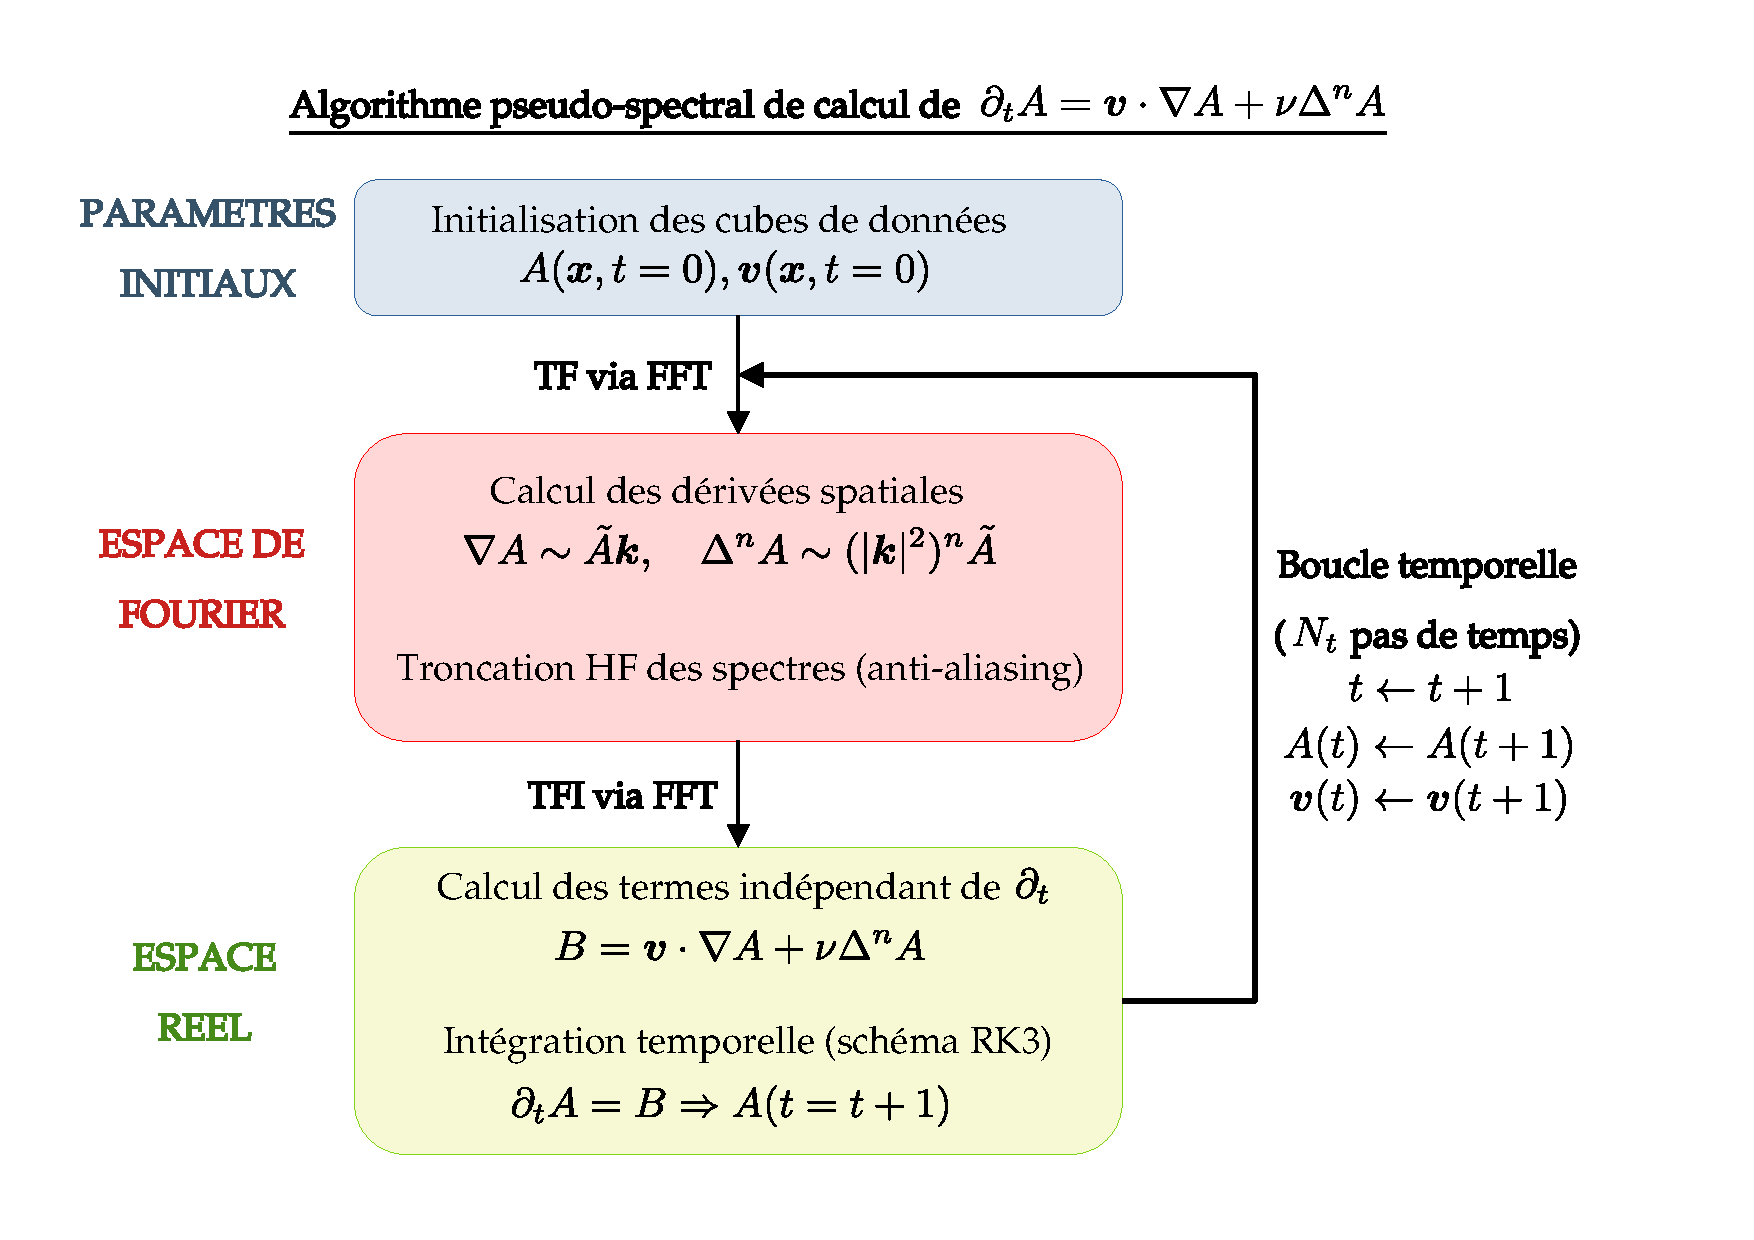
\includegraphics[width=0.9\linewidth,trim=1cm 1cm 3cm 1cm, clip=true]{./Mainmatter/Part_3/images_ch1/code_OCA}
\cprotect\caption{Algorithme d'intégration d'une équation d'évolution générique via une méthode pseudo-spectrale. Prise en compte des corrections d'anti-aliasing et d'hyperdissipation \ensuremath{\nu \Delta^n A}. TF(I) correspond à transformée de Fourier (inverse). }
\label{fig:algo_OCA}
\end{figure}

 Afin de limiter l'apparition de fort gradients et autres discontinuités liées à des instabilités numériques et induisant un arrêt brusque de la simulation, deux possibilités existent : appliquer un filtre passe-bas sur le spectre de la quantité impliquée ou un terme d'hyperviscosité dans son équation. Le choix effectué est celui de l'hyperviscosité, c'est-à-dire imposer une décroissance graduelle et de plus en plus intense du spectre de la quantité (pour plus d'informations, se référer à [\cite{borue_forced_1995,frisch_hyperviscosity_2008}]). Ce terme de dissipation numérique s'écrit $\nu \Delta^{n} X$ pour un champ $X$, avec $\nu$ une constante choisie initialement et $n$ un entier fixé à 4. $\Delta^{n}$ est effectué dans l'espace de Fourier où une décroissance du spectre en $\boldsymbol{k}^{-8}$ est donc obtenue.   
 L'existence d'un champ magnétique moyen dans les simulations induit une anisotropie spatiale de la turbulence. Sa direction est imposée suivant $\boldsymbol{e_z}$. Afin de refléter cette anisotropie, l'hyperviscosité est adaptée avec un paramètre $\alpha$ : $\Delta^{n}$ est calculé dans l'espace de Fourier tel que $(k^2_x +  k^2_y + \alpha k^2_z)^n$. Les paramètres $\nu$ et $\alpha$ sont résumés dans la \tabref{tab:setups_hd}. Avec le pas de temps $\delta t$, ils sont accordés empiriquement afin de réduire le temps de calcul, de maintenir la dissipation aux vecteurs d'onde les plus grands et d'éviter tout emballement de la simulation et l'apparition d'instabilités numériques. En termes de turbulence, l'hyperviscosité sera considérée comme le terme de dissipation évacuant l'énergie aux petites échelles.
 
 La cascade d'énergie est entretenue par un forçage permanent\footnote{Dans [\cite{hellinger_von_2018}, \cite{gomez_parallel_2005}, \cite{mininni_hybrid_2011}], une autre méthode est utilisée pour obtenir le développement d'une cascade turbulente : leurs champ de vitesse et champ magnétique sont initialisés par une superposition de modes de phases aléatoires, puis leurs simulations évoluent librement (simulations en déclin).}. Ce forçage de type antenne de Langevin (oscillateur harmonique forcé aléatoirement [\cite{tenbarge_oscillating_2014}]) injecte la somme de deux ondes de fréquences aléatoires mais proches de celle de l'onde d'Alfvén cinétique avec une amplitude correspondand au paramètre $A_f$ multiplié par un facteur aléatoire. Il est  
appliqué sur le champ de vitesse de sorte à maintenir la somme des énergies cinétique et magnétique perpendiculaires moyennes sous un niveau $E_{sup}$ et au-dessus d'un niveau $E_{inf}$ proche de $E_{sup}$. L'énergie moyenne totale est donc quasi-constante. 
Dans l'espace de Fourier, il prend la forme d'un peigne de distributions de Dirac non nulles aux vecteurs d'ondes les plus petits, tels que $\boldsymbol{k} = \{(0,\pm 1, \pm 1);(\pm 1,\pm 1, \pm 1)\}$ dans la grille numérique associée à l'espace de Fourier. L'angle d'injection de l'énergie, $\theta_i$, sert à définir la forme de la grille spatiale, un parallélépipède allongé dans la direction $\boldsymbol{e_z}$, la taille physique de cette grille est fixée telle que $L_{\perp}/L_z = \tan \theta_i$ avec $L_{\perp} = \frac{2 \pi}{k_{0\perp}} $.
 
 La taille de l'espace des échelles accessibles via ces simulations dépend de la taille de la grille spatiale. L'échelle la plus petite dans une direction est la distance minimale entre deux points de la grille dans cette direction, et l'échelle la plus grande est la moitié de la taille de la grille. Pour une étude de turbulence, on a besoin de plusieurs ordres de grandeur entre les échelles minimales et maximales. Afin d'obtenir un nombre de points suffisant, on part d'une grille de taille physique fixée mais contenant peu de points, par exemple $128^3$, puis, après avoir atteint un régime turbulent satisfaisant tel que les spectres soient stabilisés, on augmente le nombre de points et ainsi de suite jusqu'à avoir la taille voulue pour l'espace des échelles et un spectre stable. Le nombre de points idéal serait $1024^3$ ou plus, mais plus il y a de points, plus le temps de calcul augmente\footnote{Typiquement, il faut environ un mois de calcul avec $64$ processeurs pour obtenir une simulation de taille $512^2\times 1024$ dans laquelle la turbulence se serait a priori entièrement développée} et plus le calcul monopolisera de la mémoire. Similairement, le calcul du taux de cascade sera aussi plus contraignant. Un compromis doit donc être trouvé. La taille de cube minimale considérée dans le cadre des études de turbulence sera $512^3$ et une partie des simulations aura une résolution de $512^2$ dans le plan $\{\boldsymbol{e_x},\boldsymbol{e_y}\}$ et $1024$ dans la direction $\boldsymbol{e_z}$. 
 
 Les simulations utilisées et détaillées dans la \tabref{tab:setups} et la \tabref{tab:setups_hd} ont, pour la plupart, fait l'objet de l'article [\cite{ferrand_fluid_2021}]. Parmi elles, une est de résolution $1024^3$. Elle ne sera pas traitée ici car sa taille est trop importante pour le code de post-traitement implémenté et les moyens de calcul à disposition (mésocentre). 
 
 \section{Code de post-traitement pour le calcul numérique de lois exactes }
 \label{sec-312}
 
 On a vu qu'une loi exacte est une formule statistique donnant un résultat en fonction de l'échelle $\boldsymbol{\ell}$. Elle dépend de quantités évaluées localement en deux points puis combinées en une expression qui est ensuite moyennée. Une partie des termes doit ensuite être dérivée dans l'espace des échelles si aucune hypothèse d'intégration n'est effectuée. Cette méthode pourrait être implémentée directement. On considèrerait les quantités à disposition, a priori des cubes évalués en $\boldsymbol{x}$), on les translaterait de sorte à obtenir des cubes évalués en $\boldsymbol{x} - \boldsymbol{\ell}$, puis on les combinerait suivant l'expression voulue avant de les moyenner. On obtiendrait ainsi notre résultat évalué en un point de l'espace des échelles et il faudrait recommencer encore et encore afin d'obtenir l'ensemble de l'espace des échelles. Enfin, on dériverait ou intégrerait le résultat. Cet algorithme est schématisé sur la \figref{fig:algo_direct}.
 \begin{figure}[!ht]
  \centering
 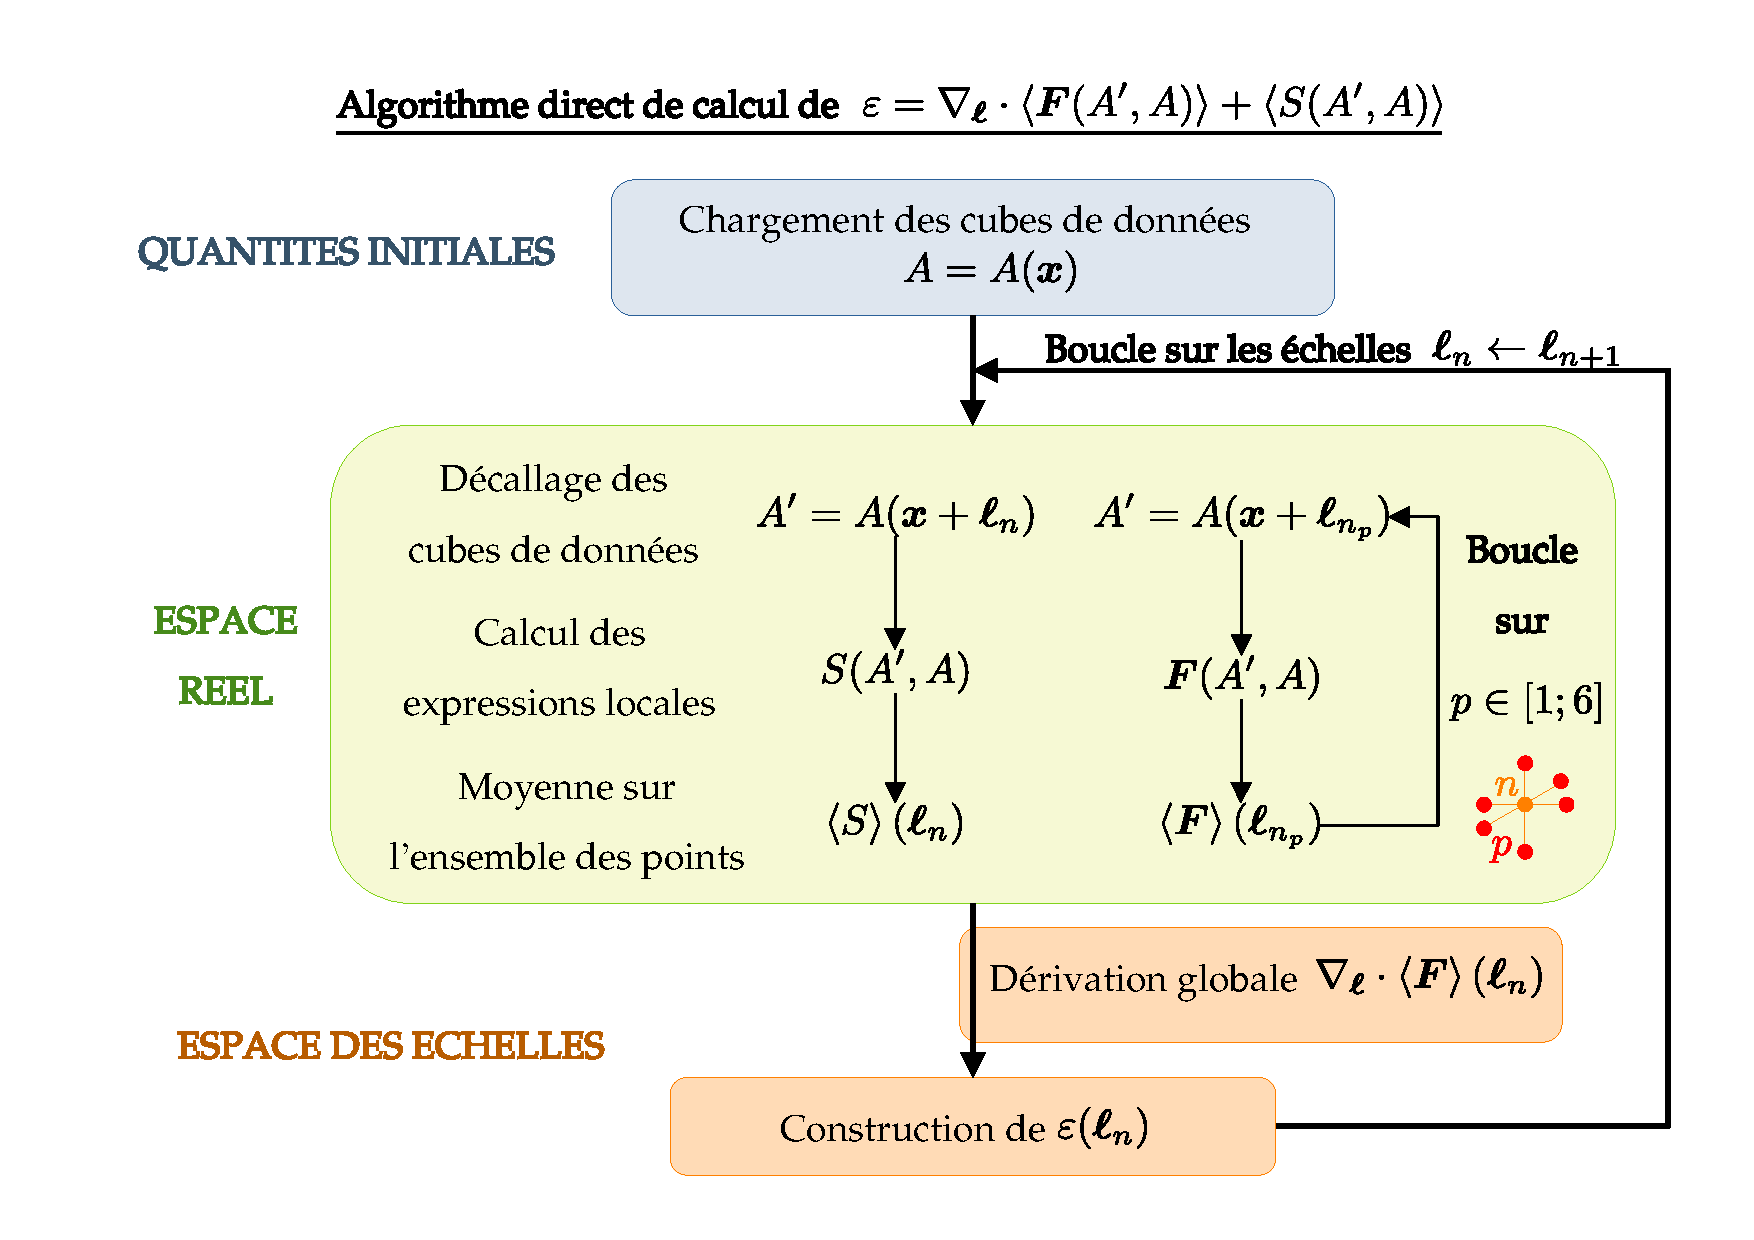
\includegraphics[width=0.9\linewidth,trim=2cm 1cm 1cm 1cm, clip=true]{./Mainmatter/Part_3/images_ch1/code_EL_direct}
 \cprotect\caption{Algorithme de calcul du taux de cascade \ensuremath{\varepsilon} via la méthode directe. Les quantités impliquées sont des quantités génériques.}
 \label{fig:algo_direct}
 \end{figure}
 
 Cette méthode est coûteuse en temps de calcul et demande des compromis. Pour réduire le temps de calcul, on peut choisir intelligemment un certain nombre de vecteurs d'échelle. Tout d'abord, on peut jouer sur la parité de la loi exacte et ne calculer que les vecteurs tels que $\ell_z \leq 0$.  \cite{ferrand_fluid_2021} et \cite{ferrand_-depth_2022} par exemple, utilisent les hypothèses d'isotropie ou d'axisymétrie de l'espace d'échelles. Dans le cas isotrope, l'espace des échelles est alors vu comme une sphère avec 73 vecteurs directeurs partant de son centre. Dans le cas axisymétrique, le découpage est similaire, mais effectué dans des disques pour chaque $\ell_z$. La divergence dans l'espace des échelles est ensuite effectuée sphériquement (resp. cylindriquement) le long de $\ell = |\boldsymbol{\ell}|$ (resp. $\ell_{\perp} = \sqrt{\ell^2_x + \ell^2_y}$) en supposant les dérivées angulaires nulles. Je n'ai pas voulu faire de même, n'étant pas convaincue de l'indépendance angulaire de la dérivée et trouvant la statistique finale faible. Une autre possibilité est de choisir les vecteurs en fonction du mode de représentation final. Si ce mode de représentation est logarithmique, on peut ne choisir qu'un nombre limité de vecteurs à grande échelle tels qu'ils soient régulièrement espacés en représentation logarithmique [\cite{manzini_local_2022}]. Un problème de cette méthode est l'irrégularité de la grille résultante. La divergence dans l'espace des échelles doit donc se faire vecteur par vecteur à partir des six échelles les plus proches (au minimum). Ce choix-là ne semblait toujours pas satisfaisant, car il implique de devoir potentiellement refaire le calcul en fonction du mode de représentation final et un biais apparaît en cas de moyenne dans l'espace des échelles. Ces compromis doivent en plus être accompagnés d'une optimisation, voire d'une parallélisation du calcul numérique. 
 
 Après maintes versions et tentatives d'optimisation de mon code de post-traitement, codé en \verb|Python| et essayant de respecter explicitement la forme de la loi exacte, j'ai décidé de changer radicalement de point de vue. 
 Mathématiquement, les opérations de corrélation et de convolution, $*$, sont liées. En effet, si l'on considère deux quantités réelles $s$ et $r$, leur fonction de corrélation peut s'écrire :
 \begin{eqnarray}
      C_{s,r}(\boldsymbol{\ell})  &=& \frac{1}{V}\iiint_V s(\boldsymbol{x} + \boldsymbol{\ell}) r (\boldsymbol{x}) d\boldsymbol{x} =  \frac{1}{V} \iiint_V s(\boldsymbol{x}) r (\boldsymbol{x} - \boldsymbol{\ell}) d\boldsymbol{x} \nonumber\\
      &=&  \frac{1}{V} \iiint_V s(\boldsymbol{x}) r (-(\boldsymbol{\ell}-\boldsymbol{x}) ) d\boldsymbol{x} = \left[ \frac{1}{V} s * \mathcal{\hat{P}}r \right](\boldsymbol{\ell}),
 \end{eqnarray}
 avec $V$ le volume d'intégration et $\mathcal{\hat{P}}$ l'opérateur de parité.
 Ainsi appliquer l'opération de corrélation entre $s$ et $r$ revient à convoluer $s$ évaluée en $\boldsymbol{x}$ avec $r$ évaluée en $-\boldsymbol{x}$.
 Une autre propriété mathématique intéressante est que l'opération de convolution correspond à un simple produit dans l'espace de Fourier et que $\mathcal{\hat{P}}r$ correspond au conjugué, $(\widetilde{r})^*$, de $\widetilde{r}$ la transformée de Fourier de $r$. Ainsi en notant $\widetilde{C}_{s,r}$ la transformée de Fourier de $C_{s,r}$ et $\text{TFI}[.]$ la transformée inverse, on obtient : 
\begin{eqnarray}
    C_{s,r}(\boldsymbol{\ell})  = \text{TFI}[\widetilde{C}_{s,r}] =  \frac{1}{V}\text{TFI}[\widetilde{s} (\boldsymbol{k}) ( \widetilde{r})^*(\boldsymbol{k})]. \quad
\end{eqnarray}
L'obtention de l'ensemble de l'espace des échelles est donc possible mais demande de développer tous les termes factorisés de la loi exacte. Par exemple, pour la fonction de structure $\left<\delta \boldsymbol{v} \cdot \delta \boldsymbol{v} \delta \boldsymbol{v}\right> $ :
\begin{eqnarray}
    \left<\delta \boldsymbol{v} \cdot \delta \boldsymbol{v} \delta \boldsymbol{v}\right> &=& \left<\boldsymbol{v'} \cdot \boldsymbol{v'} \boldsymbol{v'} - \boldsymbol{v} \cdot \boldsymbol{v} \boldsymbol{v}  + \boldsymbol{v} \cdot \boldsymbol{v} \boldsymbol{v'} + 2 \boldsymbol{v'} \cdot \boldsymbol{v} \boldsymbol{v}- \boldsymbol{v'} \cdot \boldsymbol{v'} \boldsymbol{v} - 2 \boldsymbol{v'} \cdot \boldsymbol{v} \boldsymbol{v'}\right> \nonumber\\
&=&  \text{TFI} [\widetilde{C}_{\boldsymbol{v},\boldsymbol{v} \cdot \boldsymbol{v}} - \widetilde{C}_{\boldsymbol{v} \cdot \boldsymbol{v},  \boldsymbol{v}} + 2 \widetilde{C}_{\boldsymbol{v},\boldsymbol{v}\boldsymbol{v}}  - 2 \widetilde{C}_{\boldsymbol{v}\boldsymbol{v},\boldsymbol{v}} ] \quad \nonumber  \\
&=& \frac{1}{N}  \text{TFI} [   (\widetilde{ \boldsymbol{v} \cdot \boldsymbol{v}})(\boldsymbol{\widetilde{v}})^* - \boldsymbol{\widetilde{v}} (\widetilde{\boldsymbol{v} \cdot \boldsymbol{v}})^* +2\boldsymbol{\widetilde{v}}^* \cdot (\widetilde{\boldsymbol{v} \boldsymbol{v}}) -2\boldsymbol{\widetilde{v}}\cdot (\widetilde{\boldsymbol{v} \boldsymbol{v}})^* ], \quad
\end{eqnarray}
avec $C_{\boldsymbol{v} \cdot \boldsymbol{v},  \boldsymbol{v}} = \left< \boldsymbol{v'} \cdot \boldsymbol{v'} \boldsymbol{v}\right>$, $C_{\boldsymbol{v}\boldsymbol{v},\boldsymbol{v}} = \left< \boldsymbol{v'} \cdot \boldsymbol{v} \boldsymbol{v'} \right>$ et $N$ le nombre de points moyennés (volume discret), tout en sachant que par homogénéité statistique, on a $\left< \boldsymbol{v'} \cdot \boldsymbol{v'} \boldsymbol{v'}\right> = \left< \boldsymbol{v} \cdot \boldsymbol{v} \boldsymbol{v}\right>$ et que la moyenne est distributive. Cette méthode est utilisable car il est possible de développer les expressions en des produits de deux quantités générales, une évaluée au point $\boldsymbol{x}$ et l'autre en $\boldsymbol{x'}$, et parce que la simulation est périodique. L'algorithme associé à cette méthode est schématisé sur la \figref{fig:algo_spec}.
 \begin{figure}[!ht]
  \centering
 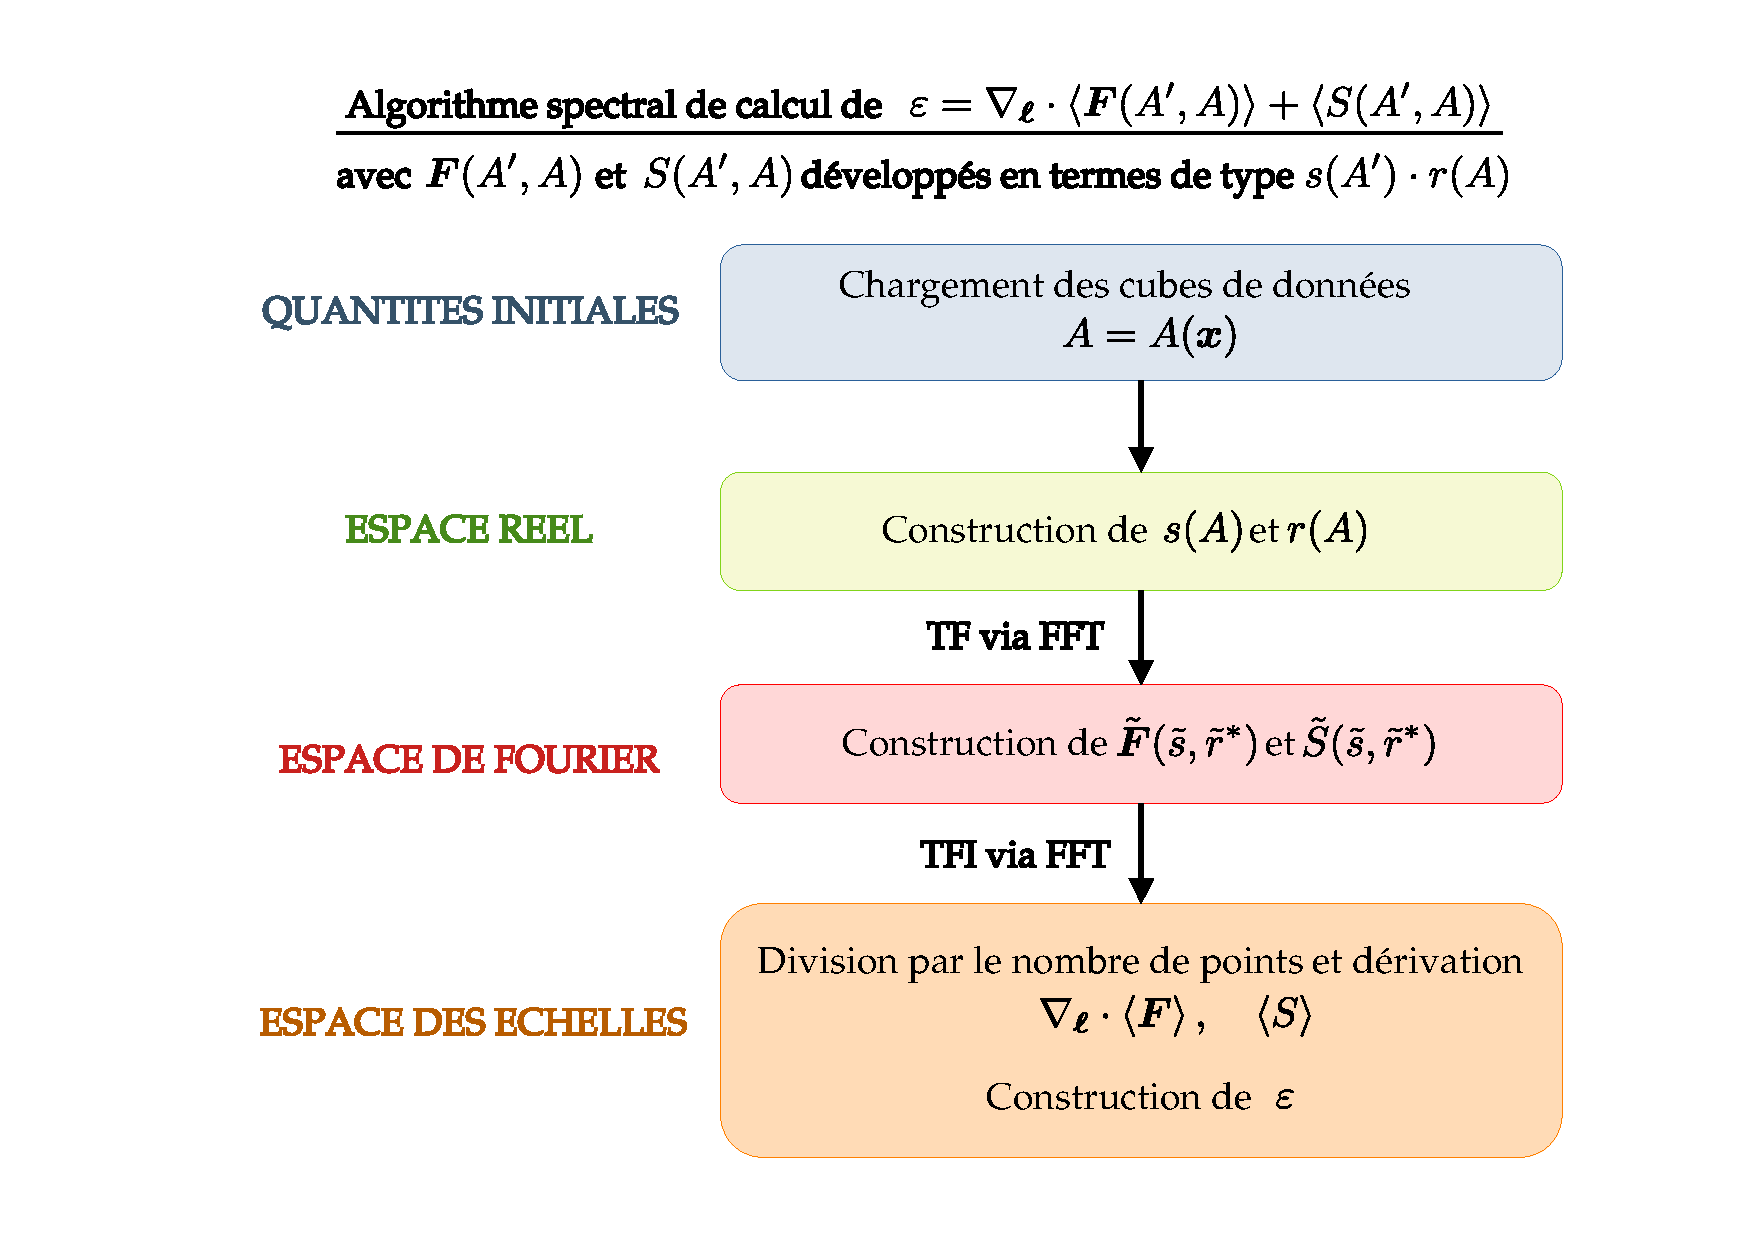
\includegraphics[width=0.93\linewidth,trim=4cm 1cm 3cm 1cm, clip=true]{./Mainmatter/Part_3/images_ch1/code_EL_spec}
 \cprotect\caption{Algorithme de calcul du taux de cascade \ensuremath{\varepsilon} via la convolution. Les quantités impliquées sont des quantités génériques.}
 \label{fig:algo_spec}
 \end{figure}
 Il demande quelques précautions lors de son implémentation, car il peut vite devenir coûteuse en mémoire, l'ensemble des termes présents dans une loi exacte devant être développé. Cependant, elle permet d'obtenir un résultat complet, indépendant du mode de représentation final des résultats. C'est donc la méthode qui a été choisie. De plus, en usant de l'algorithme de \cacro{FFT}, elle s'avère particulièrement rapide (moins de dix minutes pour calculer séparément les trois termes de \cacro{PP98} pour CGL2 par exemple).
 
 \section{Mode de représentation du résultat}
 \label{sec-313}
 \begin{figure}[!ht]
  \centering
 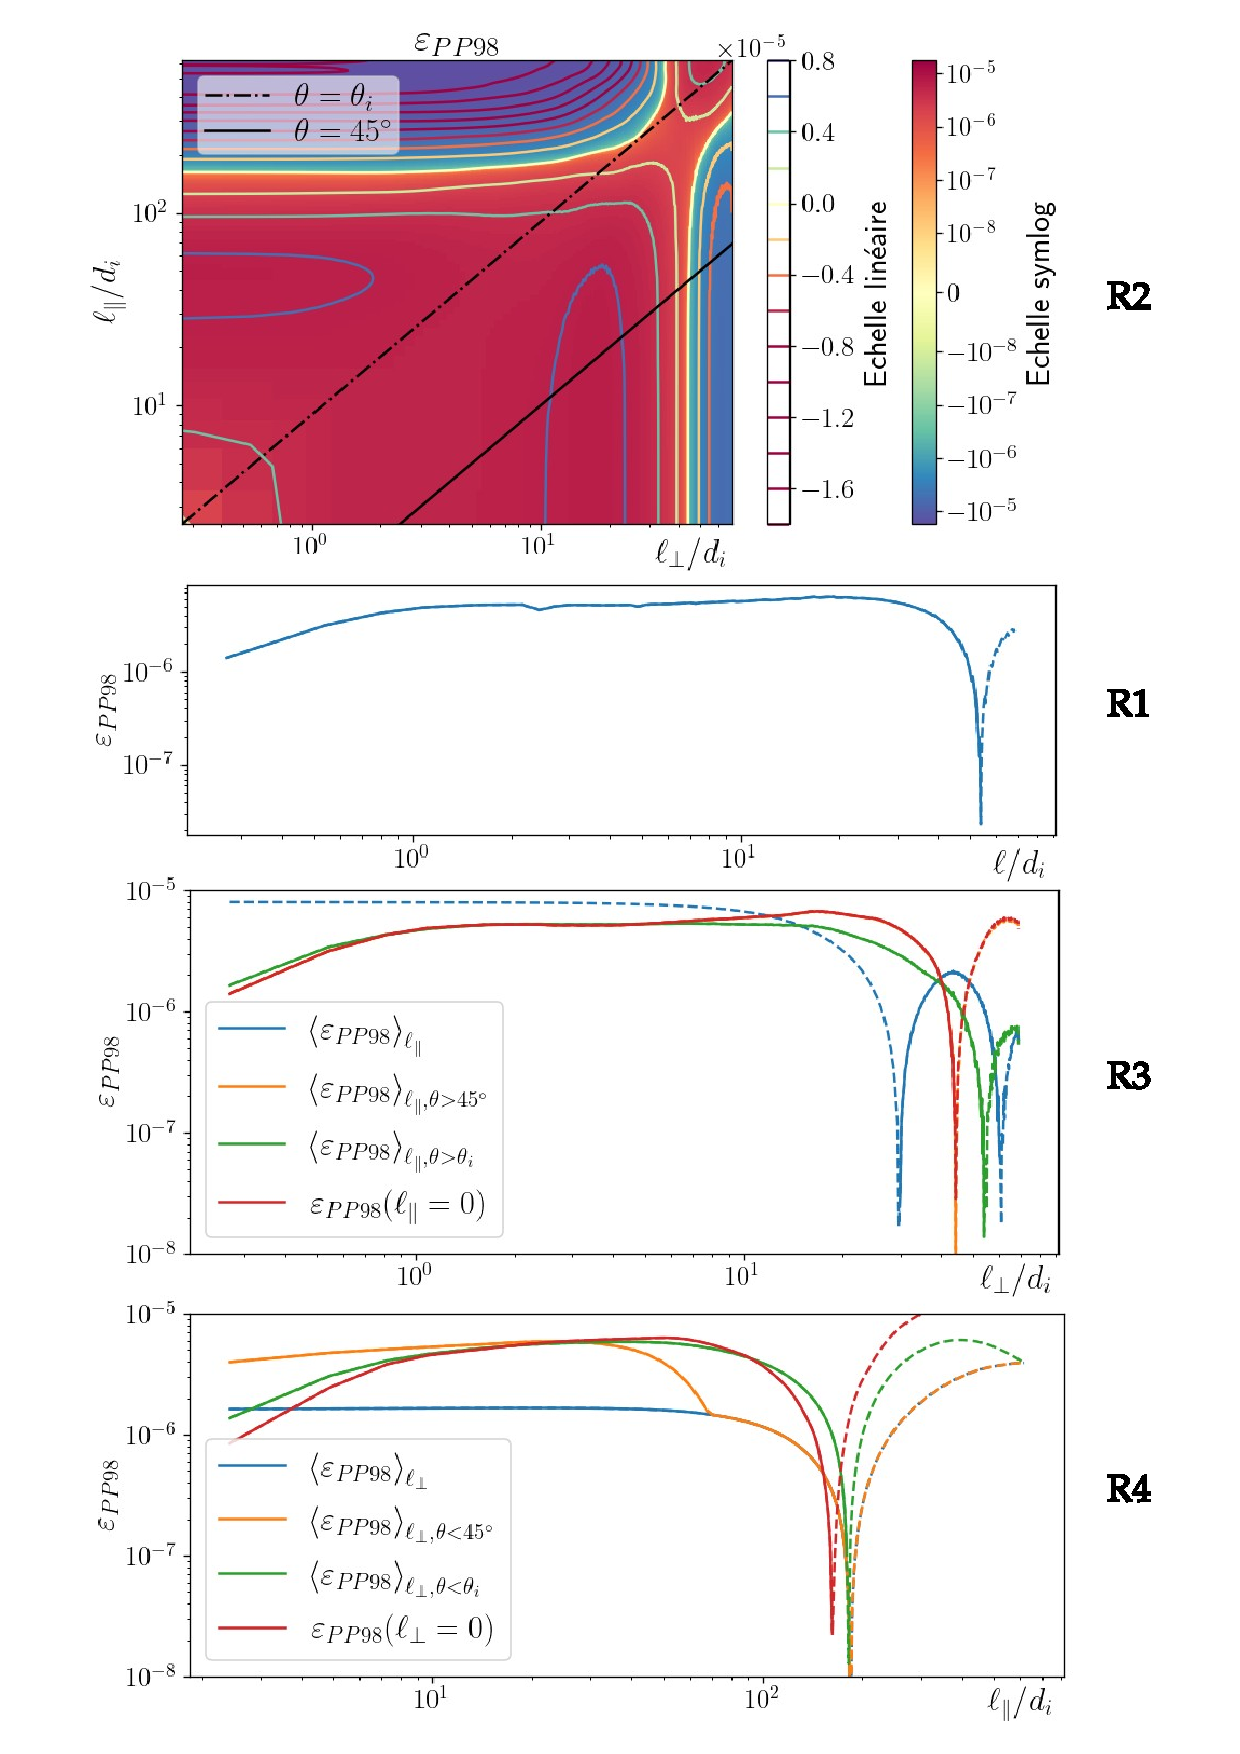
\includegraphics[width=0.75\linewidth,trim=1cm 0.5cm 1cm 0.5cm, clip=true]{./Mainmatter/Part_3/images_ch1/rep_CGL1}
 \cprotect\caption{Différents modes de représentations du taux de cascade \ensuremath{\varepsilon_{PP98}} calculé avec \cacro{PP98} dans les données de la simulation CGL1. R2 : \cacro{2D} en fonction de \ensuremath{\ell_{\perp}} et \ensuremath{\ell_{\parallel}}, avec deux échelles de couleurs, une échelle symlog, linéaire entre \ensuremath{-10^{-8}} et \ensuremath{10^{-8}} (barre de couleur continue), et une échelle linéaire (barre de couleur discontinue) et les frontières \ensuremath{\theta = \theta_i} (noire discontinue) et \ensuremath{\theta = \ang{45}} (noire continue). R1 : \cacro{1D} en fonction de \ensuremath{\ell}. R3 : \cacro{1D} en fonction de \ensuremath{\ell_{\perp}}, pour \ensuremath{\ell_{\parallel} = 0} (rouge), moyenne sur l'ensemble des \ensuremath{\ell_{\parallel}} (bleue), moyennes sur les \ensuremath{\ell_{\parallel}} tels que \ensuremath{\theta > \ang{45}} (orange) et \ensuremath{\theta > \theta_i} (vert). R4 : \cacro{1D} en fonction de \ensuremath{\ell_{\parallel}}, pour \ensuremath{\ell_{\perp} = 0} (rouge), moyenne sur l'ensemble des \ensuremath{\ell_{\perp}} (bleue), moyenne sur les \ensuremath{\ell_{\perp}} tels que \ensuremath{\theta < \ang{45}} (orange) et \ensuremath{\theta < \theta_i} (vert). Le caractère continu ou discontinu des courbes \cacro{1D} reflète le signe de \ensuremath{\varepsilon_{PP98}}.}
 \label{fig:rep_CGL1}
 \end{figure}
 Le résultat de l'algorithme de calcul par convolution est, pour chaque quantité, un parallélépipède couvrant une gamme d'échelles physiques dans la direction $\boldsymbol{e_z}$ différente de la gamme d'échelles couverte dans les directions perpendiculaires, $\boldsymbol{e_x}$ ou $\boldsymbol{e_y}$.  
 Ces gammes d'échelles couvrant différents ordres de grandeur, une représentation logarithmique est usuellement adoptée. Le caractère tridimensionnel de la grille parallélépipédique impose de choisir une méthode de réduction (\cacro{3D} vers \sacro{2D} ou \cacro{1D}) afin de pouvoir visualiser facilement les quantités. Différents types de réduction sont possibles et illustrés sur la \figref{fig:rep_CGL1} : 
 
\begin{itemize}
    \item R1 : \cacro{1D} en fonction de $\ell = |\boldsymbol{\ell}|$, en moyennant la quantité sur des coquilles de rayon moyen $\ell$,
    \item R2 : \sacro{2D} en fonction de $\ell_{\perp} = \sqrt{\ell_x^2 + \ell_y^2}$ et $\ell_{\parallel} = \ell_z$, en moyennant la quantité sur des couronnes de rayon moyen $\ell_{\perp}$ dans chaque plan perpendiculaire à $\boldsymbol{e_z}$,
    \item R3 : \cacro{1D} en fonction de $\ell_{\perp}$, en moyennant la quantité sur des coquilles cylindriques de rayon moyen $\ell_{\perp}$, la moyenne suivant $\ell_{\parallel}$ peut s'effectuer de diverses manières qui seront détaillées par la suite,
    \item R4 : \cacro{1D} en fonction de $\ell_{\parallel}$ en moyennant chaque plan perpendiculaire à $\boldsymbol{e_z}$, la moyenne suivant $\ell_{\perp}$ peut s'effectuer de diverses manières qui seront détaillées par la suite. 
\end{itemize}
 
 Sachant que la grille parallélépipédique couvre des gammes d'échelles différentes dans la direction $\boldsymbol{e_z}$ et les directions perpendiculaires (voir la carte R2 sur la \figref{fig:rep_CGL1}), notre géométrie est fondamentalement axisymétrique. La représentation de type R2 est donc la plus adaptée. L'échelle \og symlog \fg{}\footnote{Cette échelle décrit l'ensemble des nombres réels via trois représentations : $[x_0;+\infty[$ en représentation logarithmique, $]-x_0;x_0[$ en représentation linéaire (afin d'éviter la singularité du point 0), puis  $]-\infty; -x_0]$ en représentation logarithmique (en prenant l'opposé du logarithme de la valeur absolue). $x_0$ est choisi le plus petit possible.} permet de repérer les changements de signe et les ordres de grandeur couverts par $\varepsilon_{PP98}$ tandis que les courbes de niveau linéaires révèlent les variations plus spécifiques telles qu'un affaiblissement aux petites échelles ou des bosses (courbes de niveau bleues) aux échelles parallèles et perpendiculaires intermédiaires. On pourrait définir une zone inertielle entre les courbes de niveau associées à la valeur $\num{0.4}$. On remarque que cette zone semble carrée, cela est dû aux axes logarithmiques. Avec des axes linéaires, on observerait un quart d'ellipse liant $\ell_{\parallel}/d_i = \num{1e2}$ à $\ell_{\perp}/d_i \simeq \num{30} $. Le problème des cartes est la difficulté de comparer de multiples quantités. Une représentation \cacro{1D} sera donc nécessaire.

 R1 peut donner un résultat biaisé. Ainsi, sur le graphique R1 de la \figref{fig:rep_CGL1}, le résultat correspond quasiment entièrement (sauf aux très grandes échelles communes aux directions parallèle et perpendiculaire) à $\varepsilon_{PP98} (\ell_{\parallel} = 0)$ (en rouge sur le graphique R3 de la \figref{fig:rep_CGL1}). Le manque de points pour effectuer la moyenne en chaque $\ell$, induit des variations non-physiques du résultat (sursauts à intervalles réguliers sur le graphique R1 de la \figref{fig:rep_CGL1}). R3 ou R4 sont peut-être plus adaptés même si le caractère petit ou grand des échelles est défini à partir de $\ell=|\boldsymbol{\ell}|$ (resp. petit ou grand). 
 
 Cependant, visualiser la cascade via R3 en moyennant l'ensemble des $\ell_{\parallel}$ à $\ell_{\perp}$ fixé (courbe bleue) vient mixer les petits et grands $\ell$. La zone négative à grand $\ell_{\parallel}$ vient alors écraser la zone inertielle présumée et plus encore la variation des petites échelles. Le même phénomène apparaît pour R4 (courbes bleues sur les graphiques R3 et R4 de la \figref{fig:rep_CGL1}). Une autre possibilité de réduction serait de ne regarder qu'une direction $\ell_{\parallel} = 0$ pour R3 ou $\ell_{\perp} = 0$ pour R4 (courbes rouges sur les graphiques R3 et R4 de la \figref{fig:rep_CGL1}). Le résultat n'est alors pas très lisse et peu représentatif de la variation d'ensemble. 

 La troisième possibilité correspond à appliquer un filtre angulaire. En définissant $\theta$, l'angle entre $\boldsymbol{\ell}$ et $\boldsymbol{e_z}$, on pourrait considérer que les $\boldsymbol{\ell}$ contribuant à la dynamique parallèle sont les $\boldsymbol{\ell}$ quasi-parallèles tels que $\theta < \ang{45}$, et ceux contribuant à la dynamique perpendiculaire les $\boldsymbol{\ell}$ quasi-perpendiculaires tels que $\theta < \ang{45}$. La frontière $\theta = \ang{45}$ est représentée par une ligne noire continue sur la carte R2 de la \figref{fig:rep_CGL1}, et les résultats apparaissent en orange sur les graphiques R3 et R4. Pour R3, le résultat coïncide avec $\varepsilon_{PP98} (\ell_{\parallel} = 0)$. En effet, aux petites échelles, le plan tel que $\ell_{\parallel} = 0$ est la seule contribution à la moyenne. Similairement, pour R4, on assiste à un écroulement de la courbe qui rejoint $\left< \varepsilon_{PP98} \right>_{\ell_{\perp}}$ en $\ell_{\parallel} = \num{7e1}$. Cet écroulement est dû à la prise en compte de la région bleue à droite de la carte R2 pour les échelles supérieures à $\num{7e1}$. Ce filtre angulaire n'est donc pas adapté.
 
 La réduction \cacro{1D} qui sera adoptée par la suite correspond à un filtrage angulaire basé sur l'angle d'injection de l'énergie $\theta_i$. Ce dernier impose la géométrie de la grille et les gammes d'échelles accessibles. Dans l'espace des échelles, l'injection a lieu aux échelles telles que $\ell$ est maximal, c'est-à-dire dans l'angle supérieur droit de la carte R2 \figref{fig:rep_CGL1}. $\theta = \theta_i$ correspond à la diagonale représentée par une ligne noire discontinue. Appliquer cette réduction nous donne les courbes vertes des graphiques R3 et R4 de la \figref{fig:rep_CGL1}. N'y apparaissent, ni les artéfacts visibles avec R1, ni les saturations visibles sur les courbes bleues ou oranges, et elles sont plus représentatives du comportement de $\varepsilon_{PP98}$ dans l'ensemble de l'espace des échelles que les courbes rouges. On remarquera tout de même que la décroissance en allant vers les petites échelles est moins accentuée que pour les courbes rouges : les premières échelles de $\ell_{\parallel}$ (resp. $\ell_{\perp}$) différentes de $\num{0}$ sont prises en compte dans la moyenne des premiers points de $\varepsilon_{PP98}$ en fonction de $\ell_{\perp}$ (resp. $\ell_{\parallel}$).
 
%\newpage
 \section{Synthèse des méthodes et choix numériques}
 \label{synt-31}
\fcolorbox{blue}{white}{\begin{minipage}[c]{\linewidth}

\paragraph{\\Code de simulation d'un plasma turbulent (\texttt{Fortran}) : }
\begin{itemize}
\item Méthode d'intégration pseudo-spectrale (voir \figref{fig:algo_OCA}) des équations fluides.
\item Des termes d'hyperdissipation qui joueront le rôle de la dissipation aux petites échelles.
\item Un forçage permanent (dans l'espace de Fourier) de fréquences aléatoires proches de la pulsation Alfvénique et maintenant l'énergie perpendiculaire (cinétique + magnétique) du système quasiment constante.
\item Une géométrie périodique dépendant de l'angle d'injection de l'énergie $\theta_i$ et de la résolution de la grille numérique. \\
\end{itemize}
Je n'ai pas participé à l'écriture de ce code mais je l'ai utilisé pour compléter le lot de simulations analysé par \cite{ferrand_fluid_2021}.
\end{minipage}}

\fcolorbox{red}{white}{\begin{minipage}[c]{\linewidth}
\paragraph{\\Calcul des termes des lois exactes (\texttt{Python/Numpy/Scipy}) : }
Obtention rapide de {\bf l'ensemble de l'espace d'échelles accessible} grâce à une méthode de calcul spectrale basée sur le lien entre corrélation et convolution et sur la périodicité des simulations. L'algorithme est schématisé sur la \figref{fig:algo_spec}.

\paragraph{\\Visualisation des résultats (\texttt{Python/Matplotlib}) : représentation cylindrique} 
\begin{itemize}
\item Représentation \sacro{2D} en fonction de $\ell_{\parallel}$ et $\ell_{\perp}$ avec des échelles de couleurs de type chaud/froid (indiquant facilement le signe du résultat) associées aux variations logarithmiques (fond) et linéaires (courbes de niveaux) du résultat. 
\item Représentation \cacro{1D} en fonction de $\ell_{\perp}$. Réduction du résultat \sacro{2D} en moyennant sur $\ell_{\parallel}$ pour $\theta > \theta_i$.
\item Représentation \cacro{1D} en fonction de $\ell_{\parallel}$. Réduction du résultat \sacro{2D} en moyennant sur $\ell_{\perp}$ pour $\theta < \theta_i$. 
\end{itemize} 
Avec $\theta$ l'angle entre $\boldsymbol{\ell}$ et la direction moyenne du champ magnétique $\boldsymbol{e_z}$. \\

J'ai implémenté les codes de post-traitement et de visualisation des termes des lois exactes. Le code de post-traitement est disponible sur [GitHub : \cite{noauthor_paulinesimon972022-07_simu_exact_laws_nodate}].
\end{minipage}}


  Avant d'attaquer les spécificités des modèles simulés et les lois exactes associées, il est nécessaire de valider les méthodes numériques exposées dans le Chapitre \ref{ch-31} et d'en déterminer les biais. Dans la section \ref{sec-321}, les résultats de la loi exacte \cacro{IMHDH} seront comparés aux résultats de \cacro{F21}. %Dans la section \ref{sec-323}, les résultats \acs{MHD} avec pression isotrope dérivée dans le Chapitre \ref{ch-13} seront comparés aux prédictions de \ac{A18}. 
  Enfin, dans la section \ref{sec-323}, une méthode d'estimation de l'incertitude sur nos résultats sera proposée. 
  Les simulations utilisées dans ces études comparatives sont CGL1 et CGL3 (voir détail \tabref{tab:setups} et \tabref{tab:setups_hd}). Elles font partie des simulations du modèle \sacro{CGLHPe} analysées par \cacro{F21} et elles feront l'objet du Chapitre \ref{ch-33}.  

  
 
% Pour chaque simulation, une temps a été sélectionnée. À partir de cette temps, la simulation a été relancée sur quelques pas de temps rapprochés avec extraction des quantités pour chacun d'eux. Sauf exception de la  \figref{fig:compainc_t}, tous les résultats montrés dans ce chapitre correspondent à une moyenne de ces échantillons. Pour CGL1, la temps correspond au temps utilisé par F21, pour CGL3, c'est la temps précédente, \ac{F21} analysant le temps $t =\num{362}$ mais les lois exactes étant statistiquement stationnaire, on s'attend à retrouver des résultats similaires.    

 \section{Comparaison de résultats Inc-MHD-Hall avec pression isotrope et schémas numériques}
 \label{sec-321}
 
 \subsection{Comparaison avec des  résultats Inc-MHD-Hall}

 Afin de valider les méthodes et choix décrits dans le Chapitre \ref{ch-31}, nous avons calculé avec les données de CGL1 et CGL3 les quantités comparées par \cacro{F21} : 
 \begin{itemize}
     \item $\varepsilon_{MHD}$, provenant de la loi \cacro{PP98} (équation \eqref{eq:synth_inc_EL}),
     \item $\varepsilon_{Hall}$, la correction Hall incompressible (équation \eqref{eq:corr_hallinc}),
     \item $\varepsilon_{MHD-Hall} = \varepsilon_{MHD} + \varepsilon_{Hall}$, qui correspond au résultat de la loi \cacro{IMHDH} dérivée par \cite{ferrand_exact_2019}.
 \end{itemize} 
 Pour CGL1, le temps sélectionné, indiqué dans la \tabref{tab:setups}, est celui utilisée par \cacro{F21}. Ce n'est pas le cas pour CGL3, pour laquelle \cacro{F21} utilise $t =\num{357}$. Afin de ne pas apporter d'incertitude à notre comparaison en changeant les données utilisées, les résultats seront exceptionnellement donnés pour $t =\num{357}$ dans cette section. 
 
 Par conséquent, aucune différence que l'on pourra noter ne proviendra des données, des expressions des quantités ou de leur domaine de validité. Les différences entre les résultats résideront dans les schémas numériques utilisés. On a indiqué le nôtre par la mention \cacro{FEL} et celui de \cacro{F21} par \og F21\fg{}.  Nos résultats sont présentés sur la \figref{fig:compainc} par des lignes pleines et sont accompagnés de ceux des figures 3 et 5 de \cacro{F21} en pointillés. 
 
 \begin{figure}[!ht]
  \centering
 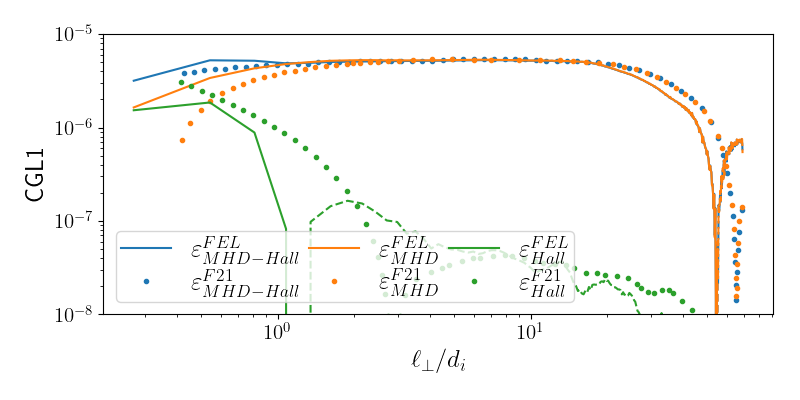
\includegraphics[width=0.85\linewidth,trim=0.5cm 0.5cm 0.5cm 0.5cm, clip=true]{./Mainmatter/Part_3/images_ch2/CGL1_compainc}
 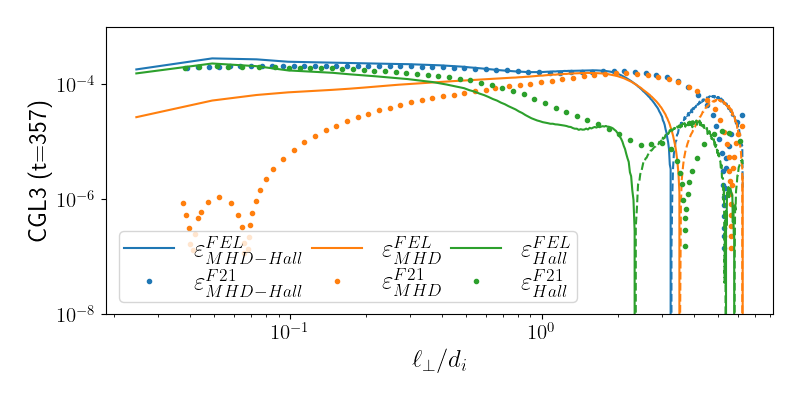
\includegraphics[width=0.85\linewidth,trim=0.5cm 0.5cm 0.5cm 0.5cm, clip=true]{./Mainmatter/Part_3/images_ch2/CGL3_compainc}
 \cprotect\caption{Mode de représentation : \cacro{1D} en fonction de \ensuremath{\ell_{\perp}} normalisé par \ensuremath{d_i}. Lignes pleines : nos résultats (avec en lignes discontinues les valeurs négatives). Pointillés : résultats extraits des figures 3 et 5 de \cacro{F21}. Bleu : \ensuremath{\varepsilon_{MHD-Hall}}. Orange : \ensuremath{\varepsilon_{MHD}}. Vert : \ensuremath{\varepsilon_{Hall}}. Haut : CGL1. Bas : CGL3 (\ensuremath{t =\num{357}}).}
 \label{fig:compainc}
 \end{figure}
 
 Tout d'abord, pour chaque simulation, on retrouve les points physiques attendus : 
 \begin{itemize}
     \item Pour CGL1 : une zone inertielle \cacro{MHD} telle que $\varepsilon_{MHD-Hall} = \varepsilon_{MHD}$ (resp. courbe bleue et orange) et une augmentation de $\varepsilon_{Hall}$ (courbe verte) en allant vers les petites échelles.
     \item Pour CGL3 : une croissance de $\varepsilon_{Hall}$, en allant vers les petites échelles, venant dominer $\varepsilon_{MHD}$ et rejoignant $\varepsilon_{MHD-Hall}$ pour former un plateau (la zone inertielle \acs{Hall}). Le croisement entre $\varepsilon_{MHD}$ et $\varepsilon_{Hall}$ a lieu près de $\ell_{\perp} = d_i$ donc à la frontière entre les zones \cacro{MHD} et \cacro{Hall}.
 \end{itemize}
 Ces résultats tendent à valider notre implémentation. D'autres tests, tels qu'une comparaison des formulations de la loi $\varepsilon_{MHD}$ (\cacro{PP98}) et celle proposée par \cite{banerjee_exact_2017}) ou la vérification des prédictions de \cite{andres_energy_2018}, ont été entrepris afin de vérifier la cohérence et le respect de la physique des lois obtenues dans la littérature. Ces résultats sont présentés dans l'Annexe \ref{an:B}.
  
 \subsection{Comparaison avec des schémas numériques à travers les résultats Inc-MHD-Hall}
 
 Les différences entre les résultats de \cacro{FEL} et \cacro{F21}, visibles sur la \figref{fig:compainc}, sont : 
 \begin{itemize}
     \item une bosse aux petites échelles pour $\varepsilon_{MHD-Hall}$ calculé avec \cacro{FEL} (ex : $\ell_{\perp}/d_i < 1$ pour le graphique sur CGL1 de la \figref{fig:compainc}),
     \item en allant vers les petites échelles, une décroissance moindre de $\varepsilon_{MHD}$ calculé avec \cacro{FEL} aux échelles $\ell < d_i$, 
     \item en allant vers les grandes échelles, une décroissance de $\varepsilon_{MHD-Hall}$ et $\varepsilon_{MHD}$ calculés avec \cacro{FEL} arrivant avant celle des quantités calculées avec \cacro{F21}.
 \end{itemize}
 Usuellement, ce qui se passe au niveau des petites échelles est attribué à la dissipation, et ce qui se passe au niveau des plus grandes échelles au forçage. Similairement,  $\varepsilon_{MHD}$ étant calculé avec la loi \cacro{PP98}, la décroissance apparaît en dehors de son domaine de validité, c'est-à-dire la zone \cacro{MHD} telle que $\ell \gg di$. Par conséquent, les différences vues n'influent pas sur l'interprétation physique. De plus, les données post-traitées et les expressions des quantités calculées étant identiques pour chaque simulation, les différences observées ne peuvent être dues qu'à une erreur de code ou aux différences présentes dans les schémas numériques utilisés. 
 
 Les différences entre les schémas numériques pouvant impacter l'estimation de nos quantités qui sont de la forme $\nabla _{\boldsymbol{\ell}} \cdot  \boldsymbol{\mathcal{F}}$ sont résumées dans la \tabref{tab:compa_F21-FEL}. Les notations associées au schéma numérique de \cacro{F21} et détaillées dans \cite{ferrand_multi-scale_2021} sont adaptées à nos notations. 
  \begin{table}[!ht]
 \begin{center}
 \begin{tabular}{ c|c|c } 
  & F21 (inspirée de \cite{taylor_recovering_2003}) & FEL (voir le Chapitre \ref{ch-31})\\
 \hline
 maillage & ensemble réduit de directions vectorielles & tous les vecteurs accessibles \\
 $\nabla_{\boldsymbol{\ell}}$ & $\frac{1}{\ell_{\perp}} \partial_{\ell_{\perp}} \left[\ell_{\perp} \left<\mathcal{F}_{\ell_{\perp}}\right>_{\phi, \ell_{\parallel}}\right]$ & $\nabla_{\boldsymbol{\ell}} \cdot \boldsymbol{\mathcal{F}}$ cartésienne \\
 filtrage des $\ell_{\parallel}$ & pour $\theta > \ang{45} $ de la grille numérique & pour $\theta > \theta_i$ \\
 $\left<\right>_{\phi,\ell_{\parallel}}$ & avant la dérivation et pondérée & après la dérivation 
 \end{tabular}
 \cprotect\caption{Différences majeures entre les schémas numériques \cacro{F21} et \cacro{FEL}. \ensuremath{\phi} correspond à l'angle présent dans le plan perpendiculaire dans un système de coordonnées cylindriques. }\label{tab:compa_F21-FEL}
 \end{center}
 \end{table}
 
 Tout d'abord, à propos du maillage de l'espace des échelles, l'utilisation d'un ensemble réduit de directions vectorielles implique l'impossibilité de calculer une divergence complète. Il faut ou interpoler, ou approximer l'opérateur de dérivation, ou calculer les quelques points adjacents pour chaque vecteur d'échelle voulu. La première solution a tendance à apporter des erreurs numériques non négligeables si le maillage interpolé n'est pas régulier, ce qui est le cas pour \cacro{F21}. Tandis que la troisième solution demande du temps de calcul supplémentaire. Finalement, la deuxième solution a été adoptée pour \cacro{F21}. N'est alors calculée que la composante transverse du flux dans chaque plan perpendiculaire au champ magnétique moyen. Ce calcul se base donc sur la symétrie des simulations, provenant du champ magnétique moyen suivant $\boldsymbol{e_z}$ et néglige les variations de la composante parallèle du flux le long de $\ell_{\parallel}$. 
 \begin{figure}[!ht]
  \centering
 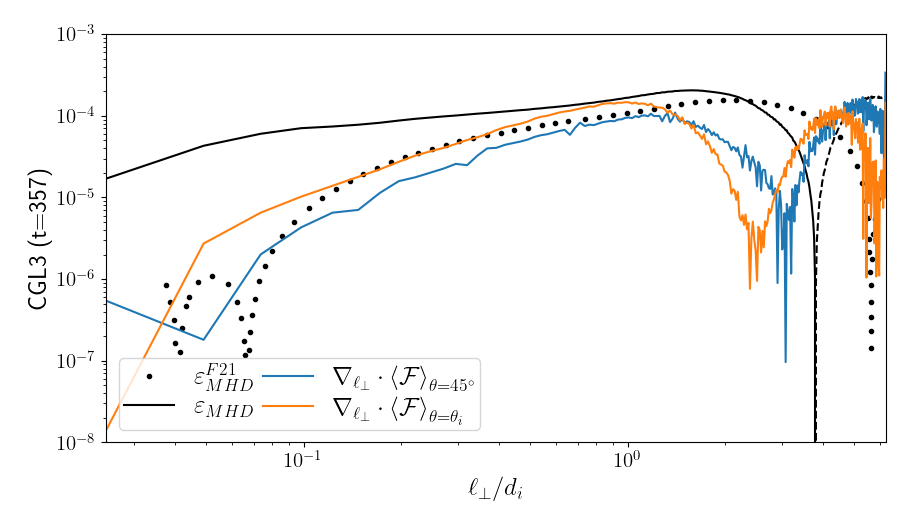
\includegraphics[width=0.9\linewidth,trim=0cm 0cm 0cm 0cm, clip=true]{./Mainmatter/Part_3/images_ch2/CGL3_compa_div}
 \cprotect\caption{Mode de représentation : \cacro{1D} en fonction de \ensuremath{\ell_{\perp}} normalisé par \ensuremath{d_i}. Simu : CGL3 (\ensuremath{t =\num{357}}). Comparaison de \ensuremath{\varepsilon_{MHD}} obtenu par \cacro{F21} (ligne noire pointillée), \cacro{FEL} (ligne noire pleine) et l'application d'une divergence transverse sur \ensuremath{\boldsymbol{\mathcal{F}}} calculés avec \cacro{FEL} et moyenné suivant deux angles \ensuremath{\theta = \ang{45}} de la boîte numérique et \ensuremath{\theta = \theta_i}. }
 \label{fig:compa_div}
 \end{figure} 
 
La \figref{fig:compa_div} illustre les effets de la variation parallèle de la composante parallèle du flux ainsi que ceux du filtrage. Le résultat \cacro{F21} (en pointillé) y est comparé à deux estimations de la divergence transverse effectuée dans nos résultats après avoir moyenné le flux dans le plan perpendiculaire et suivant les $\ell_{\parallel}$. On ne s'attend pas à retrouver exactement le résultat de \cacro{F21} mais à s'en rapprocher. La différence entre les deux estimations correspond au filtrage utilisé dans la moyenne de $\ell_{\parallel}$ : celui utilisé par \cacro{F21} en bleu, et celui que l'on utilise en orange. L'impact de l'angle de filtrage avait déjà été remarqué dans l'analyse de la \figref{fig:rep_CGL1}. On voit ici qu'il a pu influer sur le résultat de \cacro{F21} tout comme il peut influer sur le nôtre. On peut en déduire de cette figure que le poids des variations parallèles, omis par \cacro{F21}, semble avoir un impact sur nos résultats. 
 
 La différence entre nos estimations transverses et \cacro{F21} est située dans le nombre de points du maillage utilisé. Comme \cacro{FEL} prend en compte l'ensemble de l'espace des échelles, il donnera pour $\varepsilon_{MHD}$ par exemple, un résultat impacté par toutes ses variations spatiales omises par une moyenne sur un nombre réduit de vecteurs, malgré la compensation apportée par la pondération. Cet ensemble réduit d'échelles étant choisi tel des multiples de quelques vecteurs directionnels, il représentera d'autant moins les variations en s'approchant des grandes échelles.

 Il semble donc cohérent d'attribuer notre différence de comportement de $\varepsilon_{MHD}$ aux choix numériques façonnant le code de post-traitement. On peut aussi en déduire que \cacro{FEL} donne un résultat associé à la position dans l'espace \sacro{2D} plus réaliste que \cacro{F21}.
 
 \subsection{Effet du forçage sur la zone inertielle} \label{sec-322}
 
 La proximité du forçage induit de fortes variations dans le résultat à grande échelle. De plus, ici, cette injection est loin d'être stationnaire : parfois le forçage est allumé, d'autres fois, il est éteint. Sur la \figref{fig:compainc_t}, est affiché le résultat \cacro{IMHDH} pour différents temps de CGL3. 
 \begin{figure}[!ht]
  \centering
 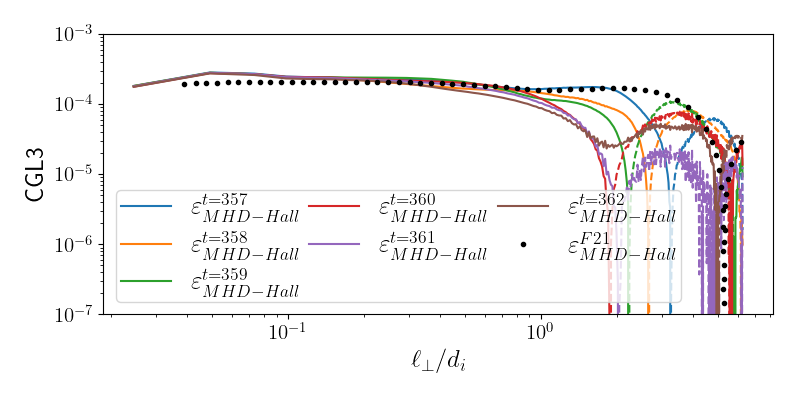
\includegraphics[width=0.9\linewidth,trim=0cm 0cm 0cm 0cm, clip=true]{./Mainmatter/Part_3/images_ch2/F19_time}
 \cprotect\caption{Mode de représentation : \cacro{1D} en fonction de \ensuremath{\ell_{\perp}} normalisé par \ensuremath{d_i}. \ensuremath{\varepsilon_{F19}} est obtenu pour divers temps \ensuremath{t} de CGL3, chaque temps correspond à une couleur. Le résultat extrait de la figure 5 de F21 est donné en pointillés noirs.}
 \label{fig:compainc_t}
 \end{figure} 
 On voit qu'en fonction du temps, l'échelle limite de la zone inertielle (telle que  $\varepsilon_{F19}$ constant) fluctue grandement. Et à $t=357$ (temps utilisé par \cacro{F21}), notre résultat (courbe bleue) montre la zone inertielle la plus large obtenue avec \cacro{FEL}. Le forçage est éteint de $t=357 $ à $t=360$ et la zone inertielle décroît petit à petit.  Puis, pour les temps suivant, il est rallumé et le plateau semble alors se reformer. On observe donc, ici, l'oscillation de l'injection. Aux échelles $\ell_{\perp}/d_i < 1$, le niveau de $\varepsilon_{F19}$ varie peu quel que soit le temps considéré. Cette observation concorde avec l'hypothèse de stationnarité statistique du taux de cascade dans la zone inertielle (ici \cacro{MHDH}). Cette hypothèse est considérée analytiquement pour obtenir des lois du type \cacro{K41} (voir synthèse \ref{synt-01}).  
 
 Le temps de simulation sélectionné impactant l'extension dans la zone de forçage de la zone inertielle, les temps de simulations indiqués dans la \tabref{tab:setups} ont été sélectionnés en prenant garde à l'état allumé ou éteint du forçage, mais cela ne signifie pas que l'extension de la zone inertielle se sera reformée. Une dernière différence, minime, n'a pas encore été abordée : celle de la variation aux petites échelles de $\varepsilon_{MHD-Hall}$. Sa signification associée à l'hyperdissipation sera abordée dans la section \ref{sec-323}.
 
 \section{Équation KHM et incertitude numérique} 
 \label{sec-323}
 
 Afin d'estimer l'incertitude sur nos résultats, nous nous sommes lancés dans la vérification de l'équation \cacro{KHM} du modèle simulé sous sa forme complète et pas seulement de la loi \cacro{K41} dont la validité est réduite à la zone inertielle. Cette estimation est permise par le travail analytique effectué en amont et décrit dans la Partie \ref{part_2}.
 
 \subsection{Calcul de la loi KHM}
 Une loi de type \cacro{KHM} peut s'écrire schématiquement (voir Chapitre \ref{ch-01}) : 
 \begin{equation}
  \label{eq:scheme_KHM_simu}   \partial_t \mathcal{R} =  \varepsilon_{NL} + \varepsilon_{D} + \varepsilon_{F}
 \end{equation}
 Nous avons vu que l'application des hypothèses de Kolmogorov donne la loi réduite de type \cacro{K41} $\varepsilon = - \varepsilon_{NL}$ (voir synthèse \ref{synt-01}). Son contenu, spécifique au modèle implémenté, sera détaillé dans les Chapitres \ref{ch-33} (\sacro{CGLHPe}) et \ref{ch-34} (\sacro{LFHPe}). 
 
 $ \partial_t \mathcal{R}$ est la dérivée temporelle de la fonction de corrélation utilisée pour obtenir la loi exacte. Dans nos études, cette fonction est  $ \mathcal{R} =\frac{1}{4} \left< (\rho'+\rho) (\boldsymbol{v'} \cdot  \boldsymbol{v} +  \boldsymbol{v'_A} \cdot  \boldsymbol{v_A}) + 2\rho' u + 2 \rho u'\right>$. Pour estimer ce terme, on va utiliser les temps consécutifs relevés dans la simulation. La dérivée temporelle sera estimée grâce à des schémas de discrétisation de type \og différences finies \fg{} d'ordre 2 : 
 \begin{itemize}
     \item décentrée vers la droite pour le premier temps $t_0$ : $ (\partial_t \mathcal{R})(t_0) = \frac{\mathcal{R}(t_0 + \delta t) - \mathcal{R}(t_0)}{\delta t}$,
     \item décentrée vers la gauche pour le dernier temps $t_{N_t}$ : $ (\partial_t \mathcal{R})(t_{N_t}) = \frac{\mathcal{R}(t_{N_t}) - \mathcal{R}(t_{N_t}-\delta t)}{\delta t}$,
     \item centrée pour les autres temps :  $ (\partial_t \mathcal{R})(t_n) = \frac{\mathcal{R}(t_{n+1}) - \mathcal{R}(t_{n-1}) }{2\delta t}$ avec $n\in ]0,N_t[$.
 \end{itemize}
 
  Le forçage présent dans nos simulations est un forçage de type antenne de Langevin appliqué sur le champ de vitesse. Par conséquent, le taux de forçage $\varepsilon_{F}$ s'écrira $\varepsilon_{F} = \frac{1}{4} \left< (\rho'+\rho) (\boldsymbol{v'} \cdot  \boldsymbol{f} + \boldsymbol{v} \cdot  \boldsymbol{f'} ) \right>$. Ce forçage dépend de deux composantes aléatoires qui font partie des quantités extraites de la simulation, elles seront notées $f_{sup}$ et $f_{inf}$. Elles permettent de construire une quantité intermédiaire $F = a_1 f_{sup} + (1-a_1) f_{inf}$ avec $a_1$ un paramètre égal à $0.5$ dans nos simulations. Les composantes de $\boldsymbol{f}$ sont alors : $f_x = \partial_y F$, $f_y = - \partial_x F$ et $f_z = 0$. 
  
  Enfin, le taux de dissipation $\varepsilon_{D}$ couvre l'ensemble des hyperdissipations présentes dans le système. Chaque quantité est associée à une hyperdissipation du type $ \nu_X \Delta^4 X$ avec $X$ quantité générique et $\Delta^4 = (\partial^2_x + \partial^2_y + \alpha \partial^2_z)^4$. On va décomposer $\varepsilon_{D}$ tel que : 
  \begin{equation}
      \varepsilon_{D} = \varepsilon^{c}_{D} + \varepsilon^{m}_{D} + \varepsilon^{ui}_{D} + \varepsilon^{ue}_{D}
  \end{equation}
  avec : 
  \begin{itemize}
      \item la contribution cinétique avec $\boldsymbol{D}_{\boldsymbol{v}} = \nu \Delta^4 \boldsymbol{v} $ et $D_{\rho} = \nu_{\rho} \Delta^4 \rho $ :
      \begin{equation}
          \varepsilon^{c}_{D} = \varepsilon^{c}_{D}(\boldsymbol{D_{v}}) + \varepsilon^{c}_{D}(D_{\rho})=   - \frac{1}{4} \left< \left(\rho'+\rho\right) \left(\boldsymbol{v'} \cdot  \boldsymbol{D_{\boldsymbol{v}}} + \boldsymbol{v} \cdot   \boldsymbol{D'_{\boldsymbol{v}}}  \right)\right>   - \frac{1}{4} \left<  \left(D'_{\rho}+D_{\rho}\right)  \boldsymbol{v'} \cdot  \boldsymbol{v}\right> 
      \end{equation}
      \item la contribution magnétique avec $\boldsymbol{D_{v_A}} = \frac{\eta}{\sqrt{\rho}} \Delta^4 (\sqrt{\rho} \boldsymbol{v_A})$ :
      \begin{eqnarray}
          \varepsilon^{m}_{D} = \varepsilon^{m}_{D}(\boldsymbol{D_{v_A}}) + \varepsilon^{m}_{D}(D_{\rho})&=& - \frac{1}{4} \left< \left(\rho'+\rho\right) \left(\boldsymbol{v'_A} \cdot  \boldsymbol{D_{v_A}} + \boldsymbol{v_A} \cdot   \boldsymbol{D'_{v_A}}  \right) \right>\nonumber \\
          &&- \frac{1}{8} \left<\left(\rho'-\rho\right) \left(\frac{D'_{\rho}}{\rho'}-\frac{D_{\rho}}{\rho}\right) \boldsymbol{v'_A} \cdot  \boldsymbol{v_A} \right>
      \end{eqnarray}  
      \item la contribution d'énergie interne ionique (gyrotrope) avec $D_u =  \frac{\nu_p}{2} \Delta^4 (2p_{\perp i } + p_{\parallel i })$ et sachant que $ \rho_i u_i = \frac{1}{2} (2 p_{\perp i } + p_{\parallel i })$:
      \begin{equation}
          \varepsilon^{ui}_{D} = \varepsilon^{ui}_{D}(D_u) + \varepsilon^{ui}_{D}(D_{\rho})=   - \frac{1}{2} \left<  \frac{\rho}{\rho'} D'_u +  \frac{\rho'}{\rho} D_u \right>- \frac{1}{2} \left< \left(\frac{ D'_{\rho}}{\rho'} - \frac{D_{\rho}}{\rho} \right)\left( \rho' u_i  -  \rho u'_i \right)   \right>  
      \end{equation}
      \item la contribution d'énergie interne électronique (isotherme) sachant que  $\rho_e u_e = \rho \ln \rho$ :
      \begin{equation}
          \varepsilon^{ue}_{D} =   - \frac{1}{2} \left<  D'_{\rho} \ln \rho +  D_{\rho} \ln \rho' +  \frac{\rho'}{\rho} D_{\rho} + \frac{\rho}{\rho'} D'_{\rho} \right>  
      \end{equation}
  \end{itemize}
 et $\nu$, $\eta$, $\nu_{\rho}$ et $\nu_p$ des constantes choisies empiriquement pour chaque simulation. Elles sont résumées dans la \tabref{tab:setups_hd}.
 
 %Sachant que dans la majorité des simulations du modèle MCGL, $\nu_{\rho} = 0$ et $\nu_p \ll \nu$, on a négligé les contributions d'énergie interne ainsi que les termes dépendant de $D_{\rho}$ dans les contributions cinétique et magnétique. 
 
 \subsection{Analyse des contributions de la loi KHM }
 
 Sur la \figref{fig:KHM}, $\varepsilon_{NL}$ (bleu) est comparé à un niveau de référence $\varepsilon_{ref} =- \partial_t \mathcal{R}  + \varepsilon_{D} + \varepsilon_{F}$ (violet), construit à partir de $\partial_t \mathcal{R}$ (rouge), $\varepsilon_{D}$ (vert) et $\varepsilon_{F}$ (orange). La différence $\zeta = \varepsilon_{ref} - \varepsilon_{NL}$ est donnée en marron. On remarque qu'elle n'est pas de l'ordre du zéro numérique ($\sim \num{e-20}$) mais environ deux ordres de grandeurs en dessous du niveau de $\varepsilon_{NL}$.  De plus, la forme des termes $\partial_t \mathcal{R}$, $\varepsilon_{D}$ et $\varepsilon_{F}$ est particulière.
 \begin{figure}[!ht]
  \centering
 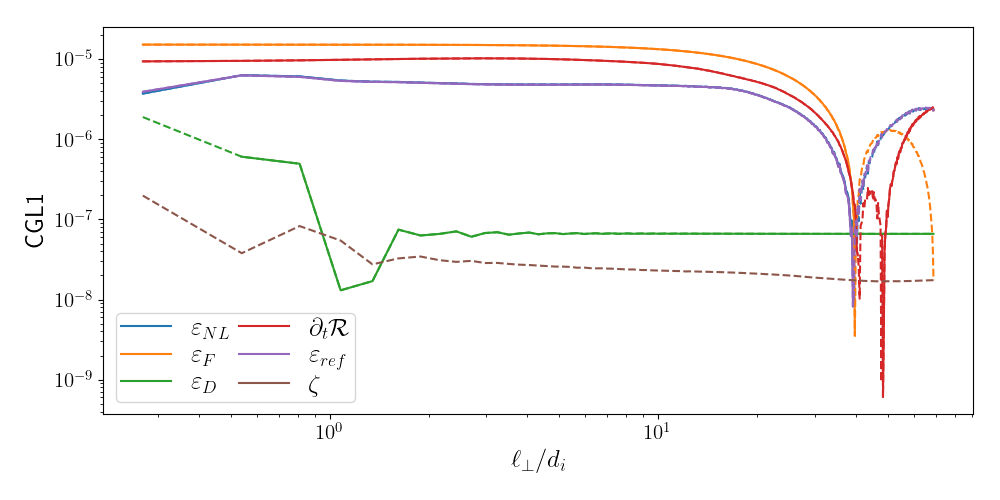
\includegraphics[width=0.9\linewidth,trim=0cm 0cm 0cm 0cm, clip=true]{./Mainmatter/Part_3/images_ch2/CGL1_1D_lperp_alll}
 %\hfill
 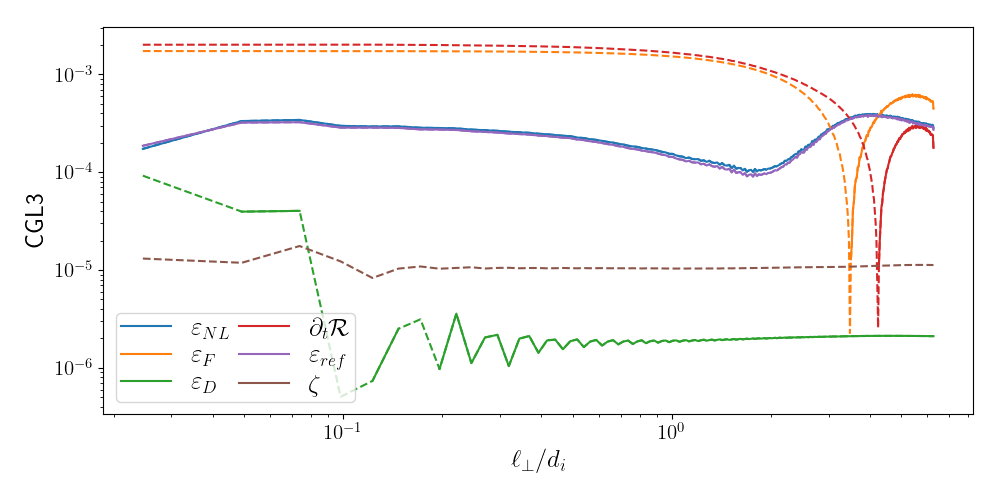
\includegraphics[width=0.9\linewidth,trim=0cm 0cm 0cm 0.5cm, clip=true]{./Mainmatter/Part_3/images_ch2/CGL3_1D_lperp_alll}
 \cprotect\caption{Détail de la loi \cacro{KHM} pour CGL1 (haut) et CGL3 (bas). Bleu : $\varepsilon_{NL}$. Orange : $\varepsilon_{F}$. Vert : $\varepsilon_{D}$. Rouge : $\partial_t \mathcal{R}$. Violet : $\varepsilon_{ref} =- \partial_t \mathcal{R}  + \varepsilon_{D} + \varepsilon_{F}$. Marron : $\zeta = \varepsilon_{ref} - \varepsilon_{NL}$. Représentation : \cacro{1D} en fonction de $\ell_{\perp}$ avec les valeurs positives en trait plein et négatives en trait discontinu. }
 \label{fig:KHM}
 \end{figure} 
 
 \paragraph{Balance des termes et forçage :  } 
 
 Tout d'abord, analysons la situation pour CGL1. Dans le Chapitre \ref{ch-01}, on a vu que : 
 \begin{equation}
     \label{eq:khm_a_verif} \varepsilon_{NL}(\boldsymbol{\ell})  = \varepsilon_{F}(\boldsymbol{\ell}) = \varepsilon_{D}(\boldsymbol{\ell} = 0) = - \varepsilon
 \end{equation}
  dans une zone inertielle où l'hypothèse de stationnarité statistique s'appliquerait. 
  
  On peut en effet identifier une gamme d'échelles $\ell_{\perp}/d_i \in \left[ \num{1}; \num{20}\right]$ telle que $\varepsilon_{NL}$ soit constant. Son niveau est alors d'environ $\num{5e-6}$. La valeur n'est pas visible ici à cause de l'échelle logarithmique mais $\varepsilon_{D}(\boldsymbol{\ell} = 0) \simeq \num{5e-6}$. Donc $\varepsilon_{NL}(\boldsymbol{\ell})  =  \varepsilon_{D}(\boldsymbol{\ell} = 0)$ semble retrouvé. Par contre, même si la constance\footnote{ Le comportement constant du terme de forçage est démontré rigoureusement dans l'annexe \ref{an:forc}.} de $\varepsilon_{F}$ est vérifiée à ces échelles, son niveau est beaucoup trop important, de l'ordre de $ \num{1.5e-5}$. Pour retrouver le niveau $\num{5e-6}$, on doit lui soustraire $\partial_t \mathcal{R}$ qui est d'environ $ \num{1e-5}$. La relation \eqref{eq:khm_a_verif} s'écrit alors dans nos simulations : 
  \begin{equation}
     \label{eq:khm_b_verif} \varepsilon_{NL}(\boldsymbol{\ell})  = \varepsilon_{F}(\boldsymbol{\ell}) - \partial_t \mathcal{R} = \varepsilon_{D}(\boldsymbol{\ell} = 0) = - \varepsilon
 \end{equation}
 
 \paragraph{Analyse du terme \ensuremath{\partial_t \mathcal{R}} :  } 
  Analytiquement, on se servait de l'hypothèse de stationnarité statistique pour annuler $\partial_t \mathcal{R}$, c'est-à-dire pour supposer qu'entre deux temps $\mathcal{R}$ ne varie pas. Puisque $\partial_t \left<E_{tot}\right>=\partial_t \mathcal{R}(\boldsymbol{\ell} = 0)$, si $\partial_t \mathcal{R}=0$ alors $\partial_t \left<E_{tot}\right>=0$.  Sauf que dans nos simulations $\left<E_{tot}\right>$ fluctue légèrement : pour les quatre temps consécutifs utilisés pour CGL1, $\left<E_{tot}\right>$, de l'ordre de $\num{1.3e0}$, augmente d'environ $\num{6e-7}$ par pas de temps. Par conséquent, $\partial_t \mathcal{R}=0$ est impossible à obtenir. C'est ce que l'on observe sur la \figref{fig:KHM} pour CGL1 comme pour CGL3. Pourtant, la convergence temporelle des résultats du calcul de loi exacte \cacro{K41} dans une certaine zone d'échelles a bel et bien été observée sur la \figref{fig:compainc_t}, et cela nous semblait une belle preuve de la stationnarité statistique de nos simulations. À première vue, ces résultats ne semblent pas compatibles. L'interprétation de ce paradoxe reste à affiner mais le comportement du $\partial_t \mathcal{R}$ instantané tel un forçage ne semble pas être une spécificité de nos simulations. En effet, \cite{ferrand_-depth_2022} trouvent un comportement similaire dans des simulations de turbulence non forcée, pour lesquelles l'énergie totale moyenne est en  décroissance perpétuelle. Dans notre cas, on pourrait peut-être interpréter le comportement du terme $\partial_t \mathcal{R}$ comme un réservoir d'énergie régulant temporellement l'injection de l'énergie dans la cascade afin que cette dernière puisse s'effectuer au taux imposé par les processus de dissipation. 
 
  \paragraph{Analyse des contributions d'hyperdissipation :  } 
  
   Un autre comportement pathologique est celui de $\varepsilon_{D}$ en fonction de $\ell$. Dans la théorie analytique, ce terme est supposé nul à toutes les échelles sauf en $\ell = 0$ à cause de l'anomalie dissipative. Dans nos simulations, son rôle est joué par les termes d'hyperdissipation, mais on s'attendrait à ce qu'ils décroissent rapidement en allant vers les grandes échelles puisque la dérivation par $\Delta^4$ impose un comportement en $k^8$ dans l'espace de Fourier. Regardons ce qu'il en est en le décomposant sur ses diverses contributions. La décomposition est présentée sur la \figref{fig:DISS}. 
 \begin{figure}[!ht]
  \centering
 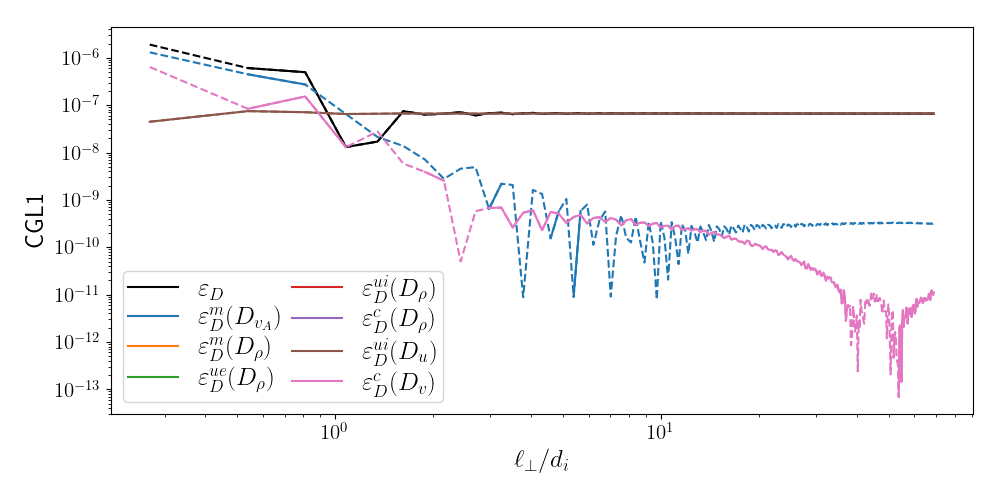
\includegraphics[width=0.9\linewidth,trim=0cm 0cm 0cm 0cm, clip=true]{./Mainmatter/Part_3/images_ch2/CGL1_1D_lperp_dissl}
 %\hfill
 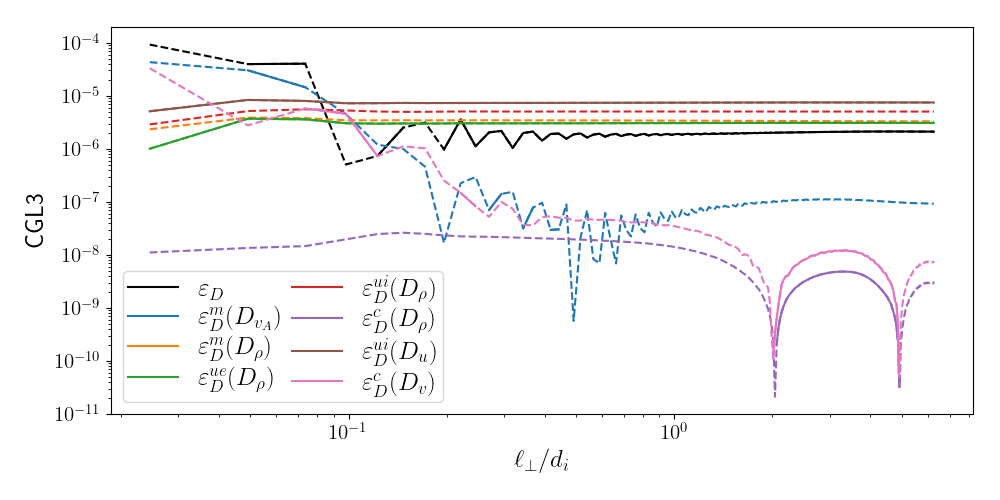
\includegraphics[width=0.9\linewidth,trim=0cm 0cm 0cm 0.5cm, clip=true]{./Mainmatter/Part_3/images_ch2/CGL3_1D_lperp_dissl}
 \cprotect\caption{Détail du terme d'hyperdissipation, $\varepsilon_{D}$ (noir), pour CGL1 (haut) et CGL3 (bas). Bleu : $\varepsilon^m_{D}(D_{\boldsymbol{v_A}})$. Orange :  $\varepsilon^m_{D}(D_{\rho})$. Vert :  $\varepsilon^{ue}_{D}(D_{\rho})$. Rouge : $\varepsilon^{ui}_{D}(D_{\rho})$. Violet :  $\varepsilon^c_{D}(D_{\rho})$ Marron :  $\varepsilon^{ui}_{D}(D_{u})$. Rose :  $\varepsilon^c_{D}(D_{v})$. Représentation : \cacro{1D} en fonction de $\ell_{\perp}$ avec les valeurs positives en trait plein et négatives en trait discontinu.}
 \label{fig:DISS}
 \end{figure}
 On y voit que chacune des contributions semble ou décroître en allant vers les grandes échelles ou rester constante. Les termes en $D_{\rho}$ (visibles seulement pour CGL3 puisque $\nu_{\rho} = 0$ pour CGL1) et $D_u$ ne montrent pas de décroissance, et la tendance en environ $\ell^{-2}$ de la décroissance de $\varepsilon^{c}_{D}(\boldsymbol{D_{v}})$ et $\varepsilon^{m}_{D}(\boldsymbol{D_{v_A}})$ avait été remarquée par \cite{ferrand_multi-scale_2021} dans le cas incompressible. La pathologie de cette pente en $-2$ y avait été identifiée et associée à une saturation mathématique de la fonction de corrélation calculée entre deux points. Cette saturation est due à une puissance de $k$ trop importante dans l'espace de Fourier et est similaire à celle relevée par \cite{cho_simulations_2009}. 
 
 Dans l'Annexe \ref{an:sat}, nous proposons une démonstration mathématique de ce phénomène en fonction du type de la fonction de corrélation, incrémentale ou non, et de la tendance du spectre dans l'espace de Fourier. On y obtient dans le cas non incrémental, pour la corrélation de deux quantités indéfinies $A$ et $B$, : 
 \begin{eqnarray}
   \label{eq:sat_noninc}  \left<A({\bf x} + \boldsymbol{\ell})  \cdot B({\bf x}) + A({\bf x})  \cdot B({\bf x} + \boldsymbol{\ell})\right> 
 \propto \left\{
     \begin{aligned}
     &\ell^{-2}& \textrm{si $m \in ]-\infty,-1[$ } \\
  &\ell^{m-1}&  \textrm{si $m \in ]-1,1[$}  \\
  &1& \textrm{si $m \in ]1,+\infty[$ } 
 \end{aligned}
 \right.%\nonumber  \\
 \end{eqnarray}
 avec $m$, la pente du spectre unidimensionnel en représentation logarithmique tel que $k^{-m}$. 
 
 Pour une fonction de corrélation incrémentale on obtient :
 \begin{eqnarray}
    \label{eq:sat_inc} \left<(A({\bf x} + \boldsymbol{\ell}) - A({\bf x}))\cdot(B({\bf x} + \boldsymbol{\ell}) - B({\bf x})) \right> 
 \propto \left\{
     \begin{aligned}
     & 1 & \textrm{si $m \in ]-\infty,1[$ } \\
 & \ell^{m-1}&  \textrm{si $m \in ]1,3[$ }  \\
 & \ell^2 & \textrm{si $m \in ]3,+\infty[$}
 \end{aligned}
 \right. .%\nonumber\\
 \end{eqnarray}
 Si l'on analyse les différentes contributions du terme de dissipation, on se rend compte que $ \varepsilon^{c}_{D}(\boldsymbol{D_{v}}) $, $ \varepsilon^{c}_{D}(D_{\rho})$, $\varepsilon^{m}_{D}(\boldsymbol{D_{v_A}}) $,
 $ \varepsilon^{ui}_{D}(D_u) $ et $\varepsilon^{ue}_{D}$ ont une forme assez proche d'une fonction de corrélation non incrémentale et $ \varepsilon^{m}_{D}(D_{\rho}) $ tandis que  $\varepsilon^{ui}_{D}(D_{\rho})$ sont plus proches d'une fonction incrémentale. 
 
 Pour une pente de spectre autour de $k^8$ ($m=-8$), une fonction de corrélation non incrémentale va saturer en $\ell^{-2}$. On retrouve ce comportement pour $ \varepsilon^{c}_{D}(\boldsymbol{D_{v}}) $ et  $\varepsilon^{m}_{D}(\boldsymbol{D_{v_A}}) $. Tandis qu'une fonction de corrélation incrémentale va saturer en $\ell^0$ (comportement retrouvé pour  $ \varepsilon^{m}_{D}(D_{\rho}) $ et  $\varepsilon^{ui}_{D}(D_{\rho})$). On retrouve aussi le comportement du terme de forçage (fonction de corrélation non incrémentale) constant loin des échelles de forçage, puisqu'un Dirac à petit $\ell$ peut-être vu comme une pente en $m = +\infty$. Ces comportements plus mathématiques que physiques sont retrouvés pour toutes les simulations. 
 
 On remarque tout de même les fortes variations des termes décroissant en $\ell^{-2}$. Ces variations sont la cause de la bosse visible aux plus petites échelles pour tous les taux $\varepsilon_{NL}$ et $\varepsilon$ calculés dans les simulations et que l'on avait remarquée dans la section \ref{sec-321}. En effet, $\varepsilon_F - \partial_t \mathcal{R} $ reste constant dans cette zone alors que la bosse apparaît dans $\varepsilon_F - \partial_t \mathcal{R} + \varepsilon_D $. Cette bosse nous indique donc les échelles auxquelles l'erreur mathématique de l'hyperdissipation impacte systématiquement $\varepsilon_{NL}$ et ses contributions.  
 
  Ce type d'erreur mathématique pourrait aussi impacter $\partial_t \mathcal{R}$, $\mathcal{R}$ étant une fonction de corrélation en deux points.
  
  \subsection{Estimation de l'erreur sur le taux de cascade  } 
 
 Les fonctions de corrélation en deux points ne sont donc pas adaptées à l'étude de la physique des termes d'hyperdissipation et de ceux inclus dans $\partial_t \mathcal{R}$ comme a pu le faire remarquer \cite{cho_simulations_2009}\footnote{La solution proposée par \cite{cho_simulations_2009} est d'augmenter le nombre de points servant au calcul de la fonction de corrélation. Une telle tâche s'annonce mathématiquement complexe et lourde dans le cadre de la théorie des lois exactes. Une autre possibilité est d'estimer précisément pour chaque contribution la puissance $m$ du spectre influant sur le résultat de chaque contribution au taux de dissipation, puis de calculer la tendance attendue en $\ell^{m-1}$ [\cite{ferrand_multi-scale_2021}].}. Par la suite, nous nous concentrerons seulement sur $\varepsilon_{NL}$ et ses contributions, mais nous garderons en mémoire les influences potentielles de ces termes.
 
 L'analyse des différentes contributions à la loi \cacro{KHM} permet ainsi d'identifier les sources d'erreurs numériques et mathématiques menant au niveau de $\zeta$. Ce dernier, de l'ordre des fluctuations de $\left< E_{tot}\right>$, reflèterait la signature de la quasi-stationnarité statistique des simulations. Aux échelles plus faibles, la saturation mathématique du calcul des fonctions de corrélation dépendant de l'hyperdissipation ainsi que sa signature\footnote{Les corrélations impliquées dans $\varepsilon_{D}$ étant d'ordre 2 et celles présentes dans les termes dominant de $\varepsilon_{NL}$ étant d'ordre 3, le reflet dans $\varepsilon_{NL}$ de l'erreur mathématique pourrait, à priori, ne pas compenser exactement l'erreur sur $\varepsilon_{D}$. } dans $\varepsilon_{NL}$ semblent impacter $\zeta$. Ce dernier correspond donc à l'incertitude systématique de notre estimation du taux de cascade, incertitude provenant des données initiales, de leur adéquation avec les hypothèses de Kolmogorov et du schéma numérique utilisé pour le calcul des termes des lois exactes. Par la suite, les contributions qui apparaîtront inférieures à $\zeta$ seront alors supposés dans la zone d'incertitude du taux de cascade total. Leur analyse devra donc être effectuée avec précautions. 
 
 Un autre point reste à éclaircir dans cette étude sur les lois du type \cacro{KHM} : la différence entre la loi obtenue en utilisant $\mathcal{R}$ et celle en utilisant une fonction incrémentale $\mathcal{S}$. La fonction $\mathcal{S}$ associée à $\mathcal{R}$ est :
 \begin{equation}
    \label{eq:scheme_khms} \mathcal{S} = \frac{1}{4} \left< \delta (\rho \boldsymbol{v}) \cdot \delta \boldsymbol{v} + \delta (\rho \boldsymbol{v_A}) \cdot \delta \boldsymbol{v_A}  + 2 \delta \rho \delta u \right>
 \end{equation}
 On a alors la relation $\mathcal{S} = \left<E_{tot}\right> - \mathcal{R}$. Sachant que $\mathcal{R}(\boldsymbol{\ell} = 0) = \left<E_{tot}\right>$, il est facile de passer de l'expression \eqref{eq:scheme_KHM_simu} à la loi :
 \begin{equation}
  \label{eq:scheme_KHMS_simu}   \partial_t \mathcal{S} = - \mathcal{E}_{NL} + \mathcal{E}_{D} + \mathcal{E}_{F}
 \end{equation}
 avec $\mathcal{E}_{NL} = \varepsilon_{NL}(\boldsymbol{\ell} = 0) - \varepsilon_{NL}$, $\mathcal{E}_{D} = \varepsilon_{D}(\boldsymbol{\ell} = 0) - \varepsilon_{D}$ et $\mathcal{E}_{F} = \varepsilon_{F}(\boldsymbol{\ell} = 0) - \varepsilon_{F}$. 
 
 \begin{figure}[!ht]
  \centering
 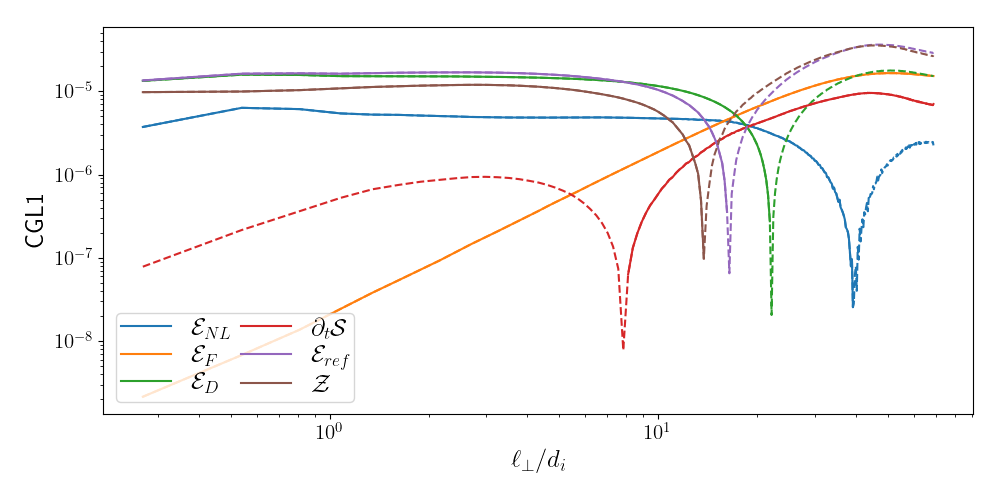
\includegraphics[width=0.9\linewidth,trim=0cm 0cm 0cm 0cm, clip=true]{./Mainmatter/Part_3/images_ch2/CGL1_1D_lperp_allSl}
 %\hfill
 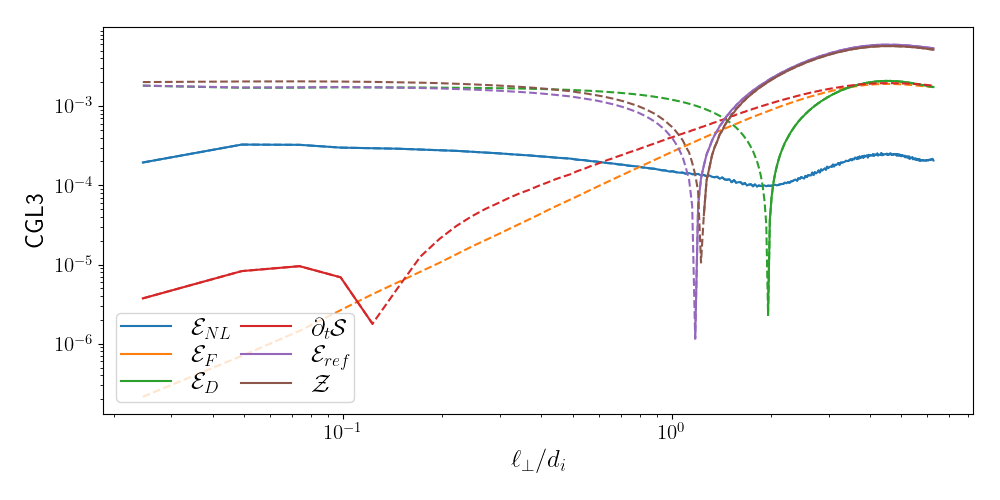
\includegraphics[width=0.9\linewidth,trim=0cm 0cm 0cm 0.5cm, clip=true]{./Mainmatter/Part_3/images_ch2/CGL3_1D_lperp_allSl}
 \cprotect\caption{Détail de la loi \eqref{eq:scheme_khms} pour CGL1 (haut) et CGL3 (bas). Bleu : \ensuremath{\mathcal{E}_{NL}}. Orange : \ensuremath{\mathcal{E}_{F}}. Vert : \ensuremath{\mathcal{E}_{D}}. Rouge : \ensuremath{\partial_t \mathcal{S}}. Violet : \ensuremath{\mathcal{E}_{ref} =- \partial_t \mathcal{S}  + \mathcal{E}_{D} + \mathcal{E}_{F}}. Marron : \ensuremath{\mathcal{Z} = \mathcal{E}_{ref} - \mathcal{E}_{NL}}. Représentation : \cacro{1D} en fonction de \ensuremath{\ell_{\perp}} avec les valeurs positives en ligne pleine et négatives en ligne dicontinue. }
 \label{fig:KHMS}
 \end{figure}
 
On notera que l'équation d'énergie totale s'écrit sous la forme $\partial_t E_{tot} + \nabla \cdot \boldsymbol{F_{tot}} = S$ avec $S$ les termes sources (dissipation et forçage), et $\boldsymbol{F_{tot}}$ le total de flux. De plus, puisque $\left<  \nabla \cdot \boldsymbol{F_{tot}} \right> = \nabla_{\boldsymbol{\ell}} \cdot \left< \boldsymbol{F_{tot}} \right> = - \left<  \nabla' \cdot \boldsymbol{F_{tot}} \right> = 0$, alors $\mathcal{E}_{NL} =  - \varepsilon_{NL}$.
 
 
 En appliquant cette transformation sur le détail de la loi \cacro{KHM} (\figref{fig:KHM}), on obtient les résultats de la  \figref{fig:KHMS}. On y remarque que le comportement des termes de forçage (orange) et de dissipation (vert) se sont inversés. $\mathcal{E}_{F}$ augmente en allant des petites vers les grandes échelles, avec une pente de facteur $2$, et $\mathcal{E}_{D} $ reste constant avant de changer de signe vers les grandes échelles. Ces comportements sont cohérents avec ceux démontrés dans les Annexes \ref{an:forc} et \ref{an:sat} (voir équations \eqref{eq:sat_noninc} et \eqref{eq:sat_inc}). Par contre, la différence $ \mathcal{Z} = \mathcal{E}_{ref} - \mathcal{E}_{NL} = (- \partial_t \mathcal{S} + \mathcal{E}_{D} + \mathcal{E}_{F}) - \mathcal{E}_{NL}$ est supérieure à $\zeta$. L'utilisation d'une fonction de corrélation incrémentale dans une étude de données de simulations semble donc amplifier l'erreur numérique et mathématique associée aux termes temporels, de dissipation et de forçage en y ajoutant l'erreur sur l'équation de $\left<E_{tot}\right>$. 
 
 %\newpage
 \section{Synthèse des tests de validation et sources d'erreurs }
 \label{synt-32}
 \fcolorbox{red}{white}{\begin{minipage}[c]{\linewidth}
 Ces études sont illustrées par les résultats obtenus pour les simulations CGL1 et CGL3. 
 
 \paragraph{Comparaison Inc-MHD-Hall avec les résultats de \cite{ferrand_multi-scale_2021} :}
 \begin{itemize}
     \item le comportement des lois \cacro{IMHDH} est retrouvé,
     \item effets de nos choix de schéma numérique. 
 \end{itemize}
 
 \paragraph{Effet du forçage sur la zone inertielle visualisée avec Inc-MHD-Hall :}
 \begin{itemize}
     \item visualisation des oscillations induites par l'injection d'energie dans le taux de cascade : extension/réduction de la zone inertielle sur environ une demi décade,
     \item visualisation de l'impact de la stationnarité statistique : amortissement des oscillations et convergence de la zone inertielle.
 \end{itemize}
 
 % \paragraph{Comparaison MHD incompressible avec la formulation de PP98 donnée par \cite{banerjee_alternative_2017} : }
 % \begin{itemize}
 %     \item comportement global retrouvé
 %     \item  différences induites par la quasi-incompressibilité des simulations
 % \end{itemize}
 
 % \paragraph{Comparaison MHD compressible avec pression isotrope avec les prédictions de \cite{andres_energy_2018} : }
 % \begin{itemize}
 %     \item  formulation f1 cohérente avec les prédictions
 %     \item validation de l'apport de f2 sur f1 et cohérence avec les prédictions
 % \end{itemize}
 
 \paragraph{Analyse de la loi KHM : }
 \begin{itemize}
     \item paradoxe sur l'hypothèse de stationnarité statistique dans les simulations,
     \item saturation mathématique apportée par l'hyperdissipation,
     \item incertitude provenant de l'utilisation de fonctions incrémentales,
     \item estimation de l'erreur numérique et mathématique sur la loi exacte totale associée au modèle simulé, noté $\zeta$. \\
 \end{itemize}
 
 {\bf Ces études valident le schéma numérique et son implémentation, et questionnent les comportements non-physiques pouvant impacter les résultats.} \\
 
 Les Annexes \ref{an:A} et \ref{an:B} contiennent des études complémentaires pour ce chapitre.
 \end{minipage}}

 Dans ce chapitre, nous attaquons le cœur de l'étude numérique dont l'objectif est de répondre à la question : quel est l'impact de la correction dépendant de l'anisotropie de pression sur le taux de cascade ? Les résultats montrés ici sont récents, préliminaires et leur interprétation est encore en cours de discussion.
 
 \section{Le modèle CGL simulé} \label{sec-331}
 
 Dans un premier lot de simulations, les ions sont décrits avec la fermeture \cacro{CGL} et les électrons avec une fermeture isotherme qui correspond à notre fermeture isotherme-isentrope. La contribution des flux de chaleur est supposée nulle. La pression électronique est définie telle que $p_e = \rho$. Le modèle général \sacro{CGLHPe} simulé dans le code versatile est donné dans la section \ref{sec-233}. Regardons à quoi il ressemble si l'on y injecte les fermetures et que l'on y applique la normalisation indiquée dans la section \ref{sec-311} et utilisée dans l'implémentation des équations. Les équations de ce modèle sont ainsi :
 \begin{eqnarray}
 \label{eq:mcgl_r} \partial_t \rho + \nabla \cdot \left(\rho \boldsymbol{v}\right) &=& 0,\\
 \label{eq:mcgl_v} \partial_t  \boldsymbol{v} + \boldsymbol{v} \cdot \nabla  \boldsymbol{v} - \frac{1}{\rho} \boldsymbol{j} \times \boldsymbol{B} + \frac{1}{\rho} \nabla \cdot \overline{\boldsymbol{P}}  &=& 0,  \\
 \label{eq:mcgl_b} \partial_t \boldsymbol{B} - \nabla \times \left( \boldsymbol{v} \times \boldsymbol{B} \right) +  d_i  \nabla \times \left( \frac{1}{\rho} \boldsymbol{j}\times \boldsymbol{B} \right) &=& 0 , \\
 \label{eq:mcgl_pperp} \partial_t  p_{\perp i }  +  \nabla \cdot \left(p_{\perp i } \boldsymbol{v} \right) +  p_{\perp i }\nabla \cdot\boldsymbol{v} -  p_{\perp i } \boldsymbol{b}\boldsymbol{b} : \nabla \boldsymbol{v}  &=& 0  ,\\
 \label{eq:mcgl_ppar} \partial_t  p_{\parallel i }  +  \nabla \cdot \left(p_{\parallel i } \boldsymbol{v} \right) +  2 p_{\parallel i }  \boldsymbol{b}\boldsymbol{b} : \nabla \boldsymbol{v}  &=& 0  ,
 \end{eqnarray}
 en notant $\overline{\boldsymbol{P}} =  \frac{\beta_0}{2} \left(\overline{\boldsymbol{P_i}} + \rho \overline{\boldsymbol{I}} \right)$ avec $\overline{\boldsymbol{P_i}} = p_{\perp i } \overline{\boldsymbol{I}} + \left(p_{\parallel i } - p_{\perp i }\right) \boldsymbol{b} \boldsymbol{b}$ le tenseur gyrotrope de pression ionique, $\boldsymbol{b} = \frac{\boldsymbol{B}}{|\boldsymbol{B}|}$ la direction du champ magnétique et $\frac{\beta_0}{2} $ une constante provenant de la normalisation des équations.
 
 L'hypothèse isotherme vient annuler la contribution $\nabla P_e$ présente dans l'équation d'induction \eqref{eq:model_simu_b} puisque : 
 \begin{equation*}
      \nabla \times \left( \frac{1}{\rho} \nabla \left(  p_e\right) \right) =  \nabla \times \left( \frac{1}{\rho} \nabla  \rho \right) = \nabla \times  \nabla \left( \ln \rho \right) = 0.
 \end{equation*}
 On s'attend donc à ce que la contribution de $\nabla P_e$ permettant de compenser l'effet de ce terme dans l'équation d'énergie totale s'annule aussi. L'énergie interne étant $\rho u = \frac{\beta_0}{2} \left(p_{\perp i } + \frac{1}{2}p_{\parallel i} + \rho \ln \rho \right) $, son équation peut en effet s'écrire :
 \begin{eqnarray}
 \label{eq:mcgl_ui} \partial_t \left(\rho u\right) + \nabla \cdot \left(\rho u \boldsymbol{v}\right) +  \overline{\boldsymbol{P}}: \nabla \boldsymbol{v} &=& 0.
 \end{eqnarray}
 
 On reconnaît dans ces équations le modèle ayant donné la loi exacte \eqref{eq:turb_cpg_elk} ainsi que le terme de \cacro{Hall} dans l'équation \eqref{eq:mcgl_b} qui indique qu'il faut prendre en compte la correction \cacro{Hall} donnée par \eqref{eq:corr_hall}. Le taux de transfert non linéaire $\varepsilon_{NL}$ obtenu, qui est aussi valable en dehors de la zone inertielle, sera noté $\varepsilon_{cgl}$. On le comparera à $\varepsilon_{iso}$ calculé avec la partie isotrope du tenseur de pression\footnote{Le comportement de $\varepsilon_{iso}$ est connu, il a été étudié par \cite{andres_energy_2018} dans le cas isotherme. Comme nous utilisons une nouvelle formulation de la loi exacte, une vérification des prédictions est détaillée dans l'Annexe \ref{an:compa_predict}.}. On s'attend, pour ces quantités, à observer une zone inertielle élargie de la zone \cacro{MHD} à la zone \cacro{Hall}. 
 La différence $\varepsilon_{\overline{\boldsymbol{\Pi}}}=\varepsilon_{cgl}-\varepsilon_{iso}$ correspond à la contribution de l'anisotropie de pression donnée par l'équation \eqref{eq:turb_cpgyr_an}. Elle sera décomposée en quatre termes : 
 \begin{itemize}
     \item un terme flux : $\nabla_{\boldsymbol{\ell}} \cdot \boldsymbol{\mathcal{F}_A} = \frac{1}{4} \nabla_{\boldsymbol{\ell}} \cdot \left< \delta \rho \delta \left(\frac{\overline{\boldsymbol{\Pi}}}{\rho}\right) \cdot \delta \boldsymbol{v} \right> $,
     \item le terme source survivant dans la limite incompressible : 
     \begin{equation*}
         \mathcal{S}_{A1} = \frac{1}{2}\left<  \delta \left(\frac{\overline{\boldsymbol{\Pi}}}{\rho}\right) : \left(\rho\nabla' \boldsymbol{v'} -  \rho'\nabla  \boldsymbol{v}\right)\right>,
     \end{equation*}
     \item le terme source compressible dépendant explicitement des fluctuations de pression : 
     \begin{equation*}
         \mathcal{S}_{A2} =  \frac{1}{4}  \left<\delta \left(\frac{\overline{\boldsymbol{\Pi}}}{\rho}\right) : \left(\rho \boldsymbol{v} \frac{\nabla' \rho'}{\rho'} -\rho'\boldsymbol{v'}  \frac{\nabla \rho}{\rho} \right)  \right>,
     \end{equation*}
     \item le terme source dépendant explicitement des fluctuations de densité : 
     \begin{equation*}
         \mathcal{S}_{A3} = - \frac{1}{4}\left< \delta \rho \left(  \boldsymbol{v} \cdot   \left(\frac{\overline{\boldsymbol{\Pi}}}{\rho}\right) \cdot  \frac{\nabla' \rho'}{\rho'} - \boldsymbol{v'} \cdot \left(\frac{\overline{\boldsymbol{\Pi'}}}{\rho'}\right) \cdot  \frac{\nabla \rho}{\rho}\right) \right>,
     \end{equation*}
 \end{itemize}
 avec $\overline{\boldsymbol{\Pi}} =  \frac{\beta_0}{2} \left(p_{\parallel i } - p_{\perp i }\right)\left( \boldsymbol{b} \boldsymbol{b} - \frac{1}{3}  \overline{\boldsymbol{I}} \right)$. Cette contribution anisotrope est entièrement portée par les ions.
 
 \section{Étude de la loi CGL-MHD-Hall-\ensuremath{\nabla P_e} dans les simulations CGL1, CGL2, CGL3}
 \label{sec-332} 
 
 Tout d'abord, nous avons entrepris l'analyse des simulations CGL1, CGL2 et CGL3.
 Ce sont les simulations \sacro{CGLHPe} analysées dans l'article de \cite{ferrand_fluid_2021}, leurs paramètres sont résumés dans la \tabref{tab:setups} et la \tabref{tab:setups_hd}. Ces trois simulations sont initialisées telles que $a_{pi} = 1$. 
 
 \subsection{Loi globale et contribution de l'anisotropie de pression}
 La \figref{fig:trip_CGL1-2} (CGL1 et CGL2) et la \figref{fig:trip_CGL3} (CGL3) contiennent des triptyques associés à chaque simulation et permettant de comparer les taux de cascade $\varepsilon_{iso} $ et  $\varepsilon_{cgl}$. La différence des deux $\varepsilon_{\overline{\boldsymbol{\Pi}}} $ est représentée en \sacro{2D} en fonction de $\ell_{\perp}$ et $\ell_{\parallel}$, et est projetée dans les représentations \cacro{1D} sous la forme de courbe verte. Sur les représentations \cacro{1D}, sont ajoutés $\varepsilon_{cgl}$ en bleu, $\varepsilon_{iso}$ en orange et le niveau d'incertitude $\zeta$ en gris qui reste assez éloigné des autres quantités.
 
 \begin{figure}[!ht]
  \centering
  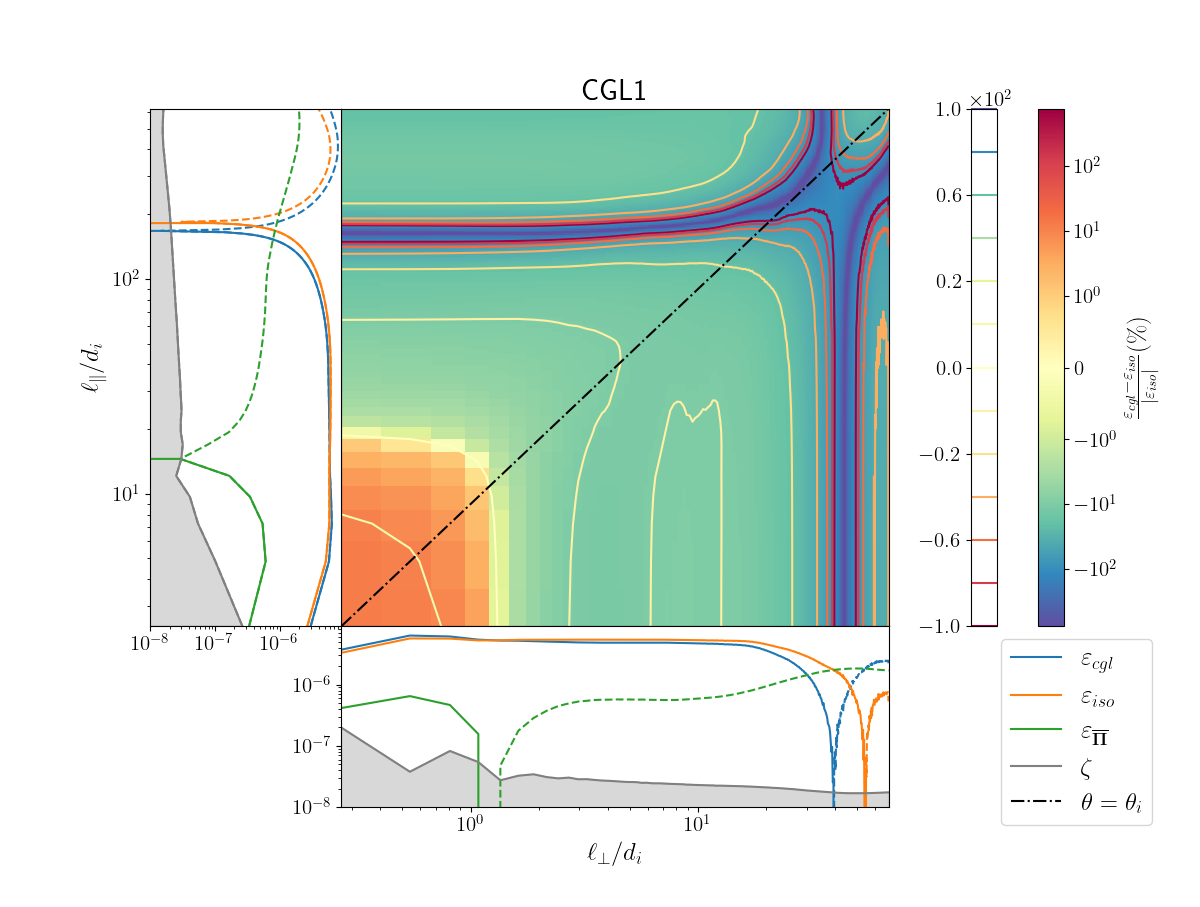
\includegraphics[width=0.95\linewidth,trim=1cm 0cm 0cm 2cm, clip=true]{./Mainmatter/Part_3/images_ch3/CGL1_panel_isocgl_percent}
 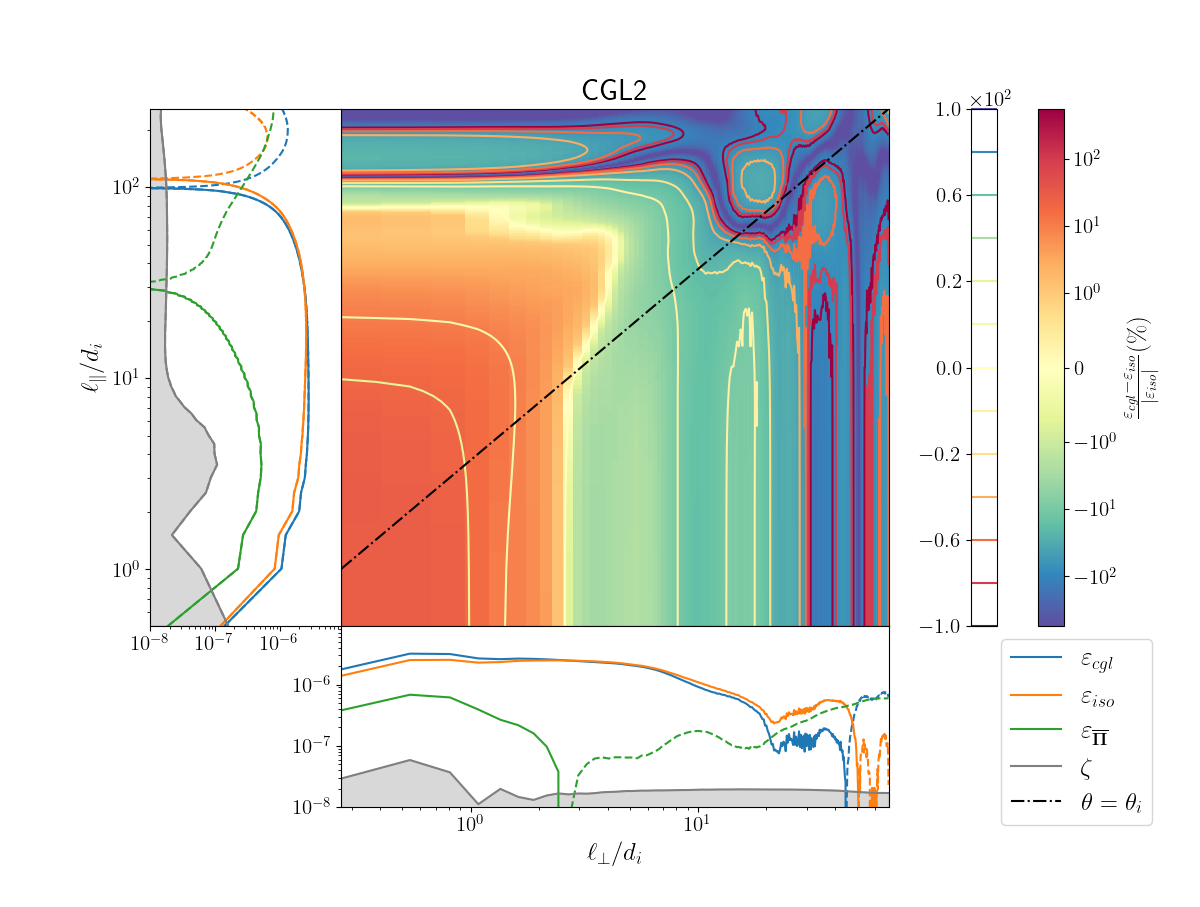
\includegraphics[width=0.95\linewidth,trim=1cm 0cm 0cm 2cm, clip=true]{./Mainmatter/Part_3/images_ch3/CGL2_panel_isocgl_percent}
 \cprotect\caption{Simu : CGL1 et CGL2. Représentation \cacro{2D} en fonction de \ensuremath{\ell_{\perp}} et \ensuremath{\ell_{\parallel}} de \ensuremath{\varepsilon_{cgl}-\varepsilon_{iso}} par rapport à \ensuremath{|\varepsilon_{iso}|} en \ensuremath{\%}, entourée des représentations \cacro{1D} en fonction de \ensuremath{\ell_{\perp}} (bas) et \ensuremath{\ell_{\parallel}} (gauche) de \ensuremath{\varepsilon_{iso}} (orange), \ensuremath{\varepsilon_{cgl}} (bleu), \ensuremath{\varepsilon_{\overline{\boldsymbol{\Pi}}}} (vert) et \ensuremath{\zeta} (gris). }
 \label{fig:trip_CGL1-2}
 \end{figure}
 \begin{figure}[!ht]
  \centering
 % 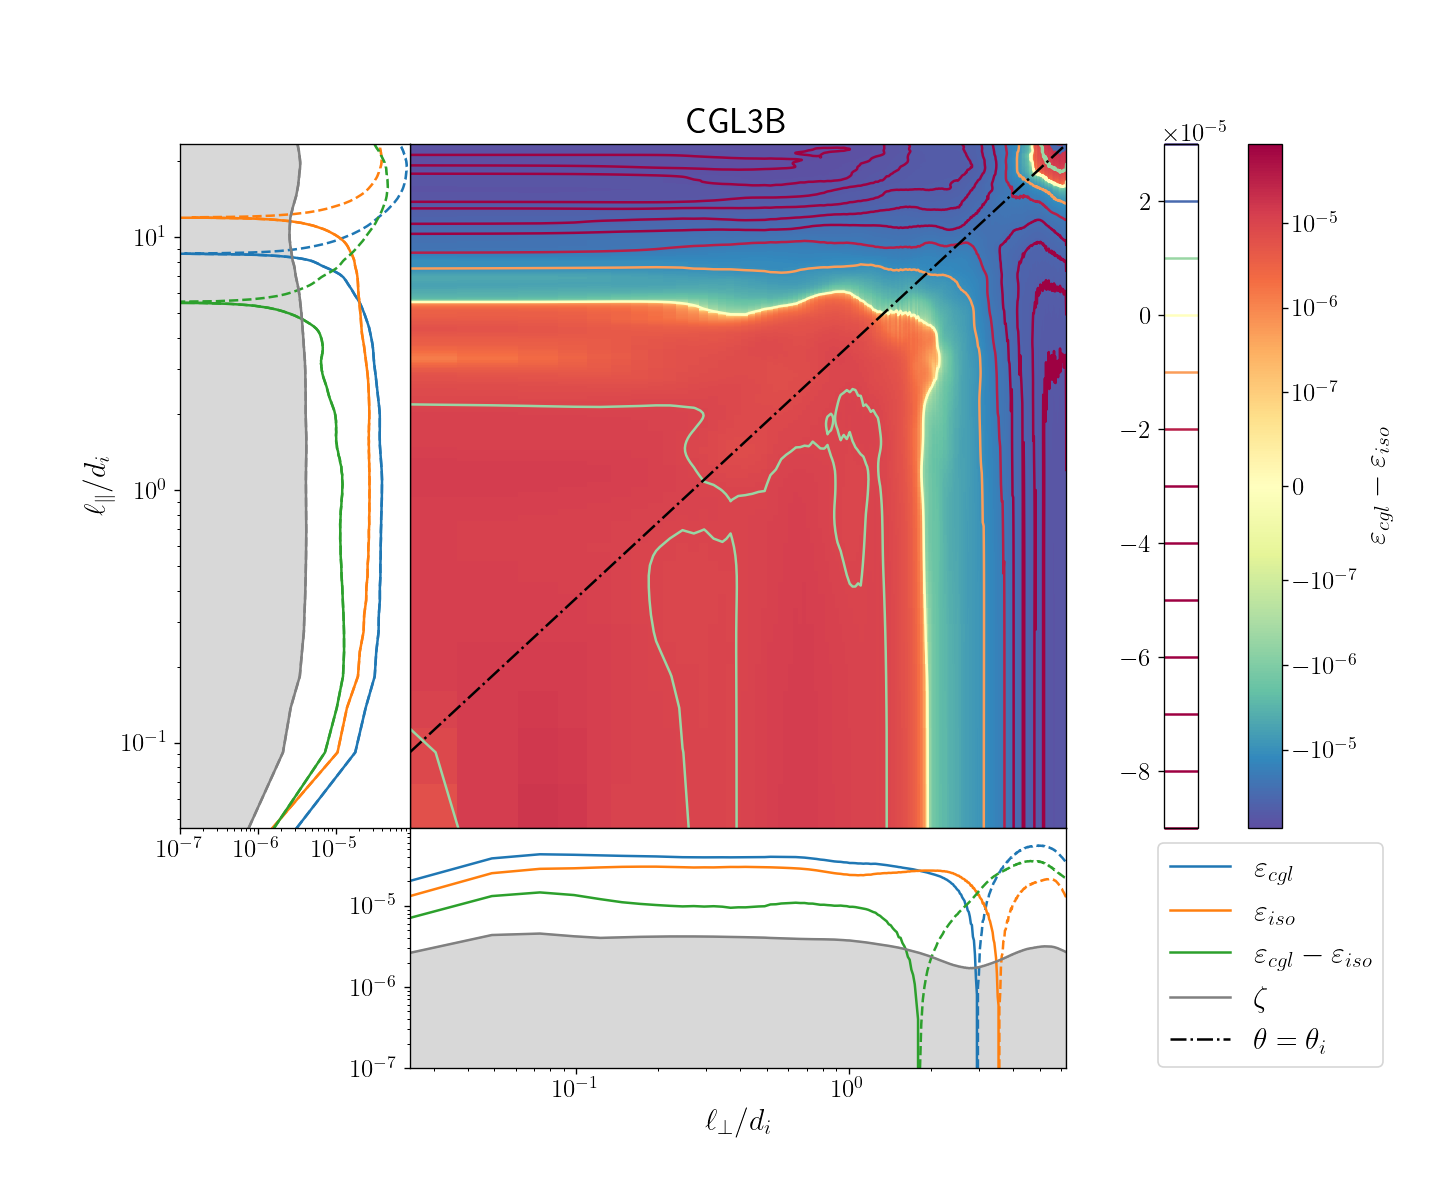
\includegraphics[width=0.95\linewidth,trim=0cm 2cm 0cm 3.5cm, clip=true]{./Part_3/images_ch3/CGL3B_panel_isocgl}
 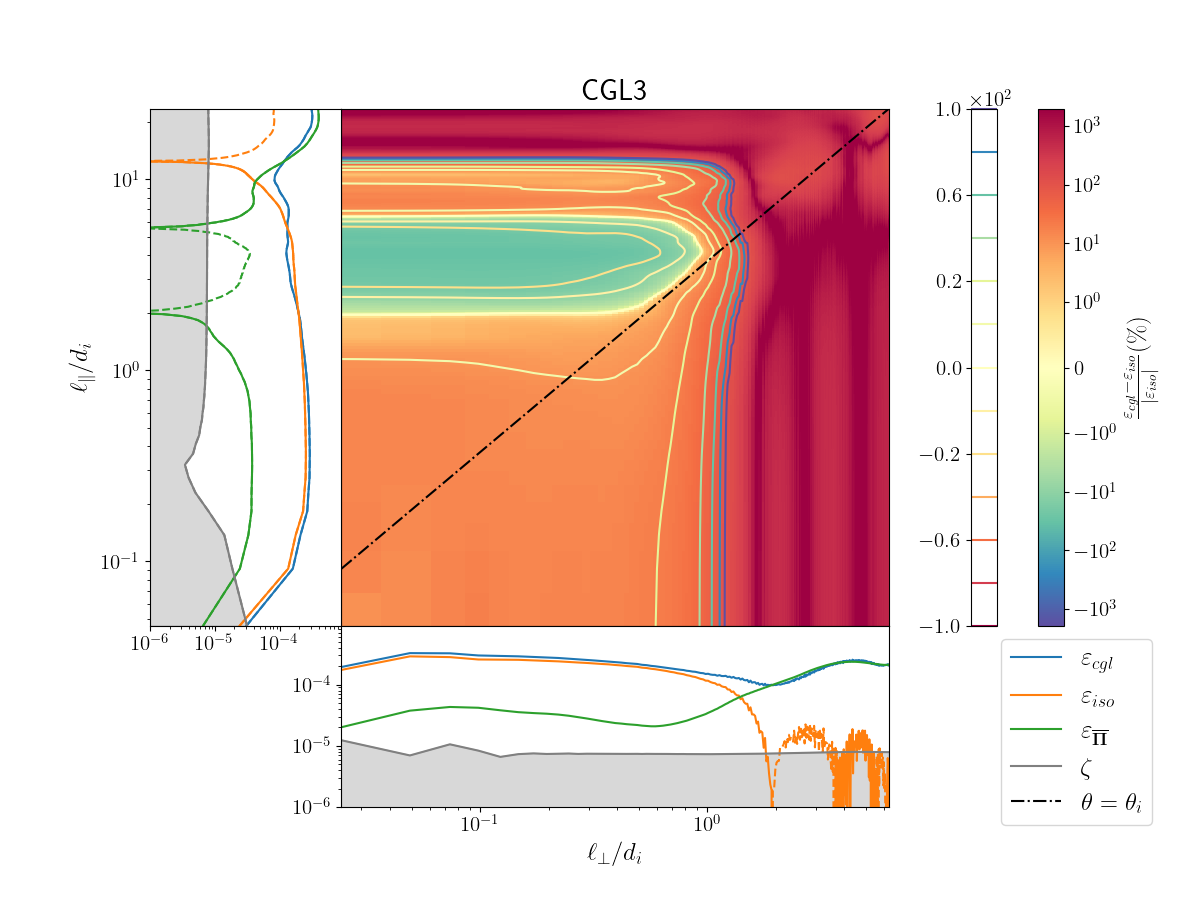
\includegraphics[width=0.95\linewidth,trim=1cm 1cm 0cm 2cm, clip=true]{./Mainmatter/Part_3/images_ch3/CGL3_panel_isocgl_percent}
 \cprotect\caption{Simu : CGL3. Représentation \cacro{2D} en fonction de \ensuremath{\ell_{\perp}} et \ensuremath{\ell_{\parallel}} de \ensuremath{\varepsilon_{cgl}-\varepsilon_{iso}} par rapport à \ensuremath{|\varepsilon_{iso}|} en \ensuremath{\%}, entourée des représentations \cacro{1D} en fonction de \ensuremath{\ell_{\perp}} (bas) et \ensuremath{\ell_{\parallel}} (gauche) de \ensuremath{\varepsilon_{iso}} (orange), \ensuremath{\varepsilon_{cgl}} (bleu),  \ensuremath{\varepsilon_{\overline{\boldsymbol{\Pi}}}} (vert) et \ensuremath{\zeta} (gris).}
 \label{fig:trip_CGL3}
 \end{figure}
 
 À partir de ces figures, on peut définir une zone inertielle où $\varepsilon_{cgl}$ sera quasi-constant pour chaque simulation. Pour CGL1, elle s'étend entre $\ell_{\perp} \in [\num{1};\num{20}]$ et $\ell_{\parallel} \in [\num{10};\num{60}]$, pour CGL2 entre $\ell_{\perp} \in [\num{1};\num{6}]$ et $\ell_{\parallel} \in [\num{2};\num{40}]$, et pour CGL3 entre $\ell_{\perp} \in [\num{0.1};\num{1}]$ et $\ell_{\parallel} \in [\num{0.2};\num{2}]$. Les variations que l'on pourra observer en dehors de ces domaines seront sous influence dissipative ou dans la zone de forçage. On remarque que la zone inertielle de CGL1 et CGL2 couvrent les échelles \cacro{MHD} et celle de CGL3, les échelles \cacro{Hall}. Dans ces zones, la contribution de $\varepsilon_{\overline{\boldsymbol{\Pi}}}$ au taux de cascade totale est en valeurs absolues d'environ $\SI{10}{\%}$ de $\varepsilon_{iso}$ pour CGL1 et CGL3, et entre $\SI{2}{\%}$ et $\SI{20}{\%}$ pour CGL2 (on prendra la valeur médiane : $\SI{10}{\%}$). Ce niveau reste donc constant. 
 
 Cependant, une différence de taille apparaît autour des grandes échelles de CGL3 (\figref{fig:trip_CGL3}) : $\varepsilon_{\overline{\boldsymbol{\Pi}}}$ augmente autour de $\num{10}$ fois la valeur de $\varepsilon_{iso}$. En pratique, on ne regarde pas ce qu'il se passe à ces échelles car elles sont impactées par l'injection d'énergie dans la cascade qui a tendance à faire fortement fluctuer les résultats provenant des lois calculées jusqu'à présents dans la littérature. Donc a priori, cette augmentation n'aurait pas un sens physique généralisable et serait plus spécifique à l'outil numérique. Pourtant, contrairement à l'impact du forçage observé dans la section \ref{sec-322}, il n'est pas oscillant et il provient spécifiquement de la contribution anisotrope. On s'est alors posé la question de son origine et de sa nature.
 
 Une autre différence est visible. Sur la représentation \sacro{2D} de CGL3 (\figref{fig:trip_CGL3}), la contribution anisotrope est positive quasiment partout à l'exception d'une \og bulle \fg{} accrochée à la direction parallèle. Tandis que pour CLG1 et CGL2 (\figref{fig:trip_CGL1-2}), un changement de signe de $\varepsilon_{\overline{\boldsymbol{\Pi}}}$ dans la zone inertielle \cacro{MHD} ($\ell > d_i$) semble indiquer une échelle caractéristique. Aux plus petites échelles, il est positif et puis devient négatif. L'emplacement de ce changement de signe est situé autour de $\ell^{s}_{\perp} \sim 2d_i$ dans la direction perpendiculaire. Dans la direction parallèle, le changement de signe a lieu en $\ell^{s}_{\parallel} \sim 20d_i$ pour CGL1, $\ell^{s}_{\parallel} \sim 80d_i$ pour CGL2. Trois éléments pourraient potentiellement expliquer ces observations. 
Tout d'abord, en présence d'un champ magnétique, le développement de la cascade est anisotrope comme on peut facilement le visualiser sur les cartes de \cite{manzini_local_2022}. Cela pourrait venir expliquer l'observation $\ell^{s}_{\perp}<\ell^{s}_{\parallel}$. Ensuite, l'angle d'injection $\theta_i$ étant inférieur à $\ang{45}$, l'énergie n'est pas injectée isotropiquement dans la simulation. Il diffère d'ailleurs entre CGL1 ($\ang{7}$) et CGL2-CGL3 ($\ang{15}$). Si le premier élément est validé, cela pourrait impliquer que l'angle d'injection pourrait venir contrer ou amplifier l'anisotropie de $\varepsilon_{\overline{\boldsymbol{\Pi}}}$. Enfin, entre CGL2 et CGL3, la gamme d'échelles diffère ainsi que le niveau énergétique ($E_{sup}$), plus important pour CGL3.

 Le comportement dans la direction parallèle semblant plus complexe que celui de la direction perpendiculaire, on s'est focalisé sur la compréhension de cette dernière.
 Puisque le changement de signe a lieu près de la zone \cacro{Hall}, on s'est demandé si le comportement de CGL2 et celui de CGL3 ne se complétaient pas : l'augmentation présente dans CGL3 serait-elle le début d'une bosse qui ensuite se répercuterait aux échelles  \cacro{MHD} où sa diminution irait jusqu'à engendrer un croisement de $\varepsilon_{cgl}$ et $\varepsilon_{iso}$ et un changement de signe de $\varepsilon_{\overline{\boldsymbol{\Pi}}}$ ? Ce point est intéressant, car une telle bosse pourrait être la signature d'instabilités qui viendraient injecter de l'énergie aux échelles ioniques. Cette première question est mise en doute par le comportement de CGL1 et CGL2 : une augmentation similaire semble apparaître dans $\varepsilon_{\overline{\boldsymbol{\Pi}}}$  mais avec un signe opposé et une intensité moindre n'influant que très peu sur $\varepsilon_{cgl}$. Si c'est bien le même effet que pour CGL3, il serait alors accroché aux échelles de forçage. 
 Plus de questions que de réponses émergent donc de ces simulations, elles ont emmené l'analyse dans diverses directions nécessitant de nouvelles simulations : 
 \begin{itemize}
     \item le niveau de la zone inertielle changera-t-il si l'on initialise la simulation avec une pression anisotropique ($a_{piI} \neq 1$) ? 
     \item l'augmentation à grande échelle est-elle accrochée aux échelles de forçage ?
    \item le changement de signe de  $\varepsilon_{\overline{\boldsymbol{\Pi}}}$ est-il lié à la proximité de la frontière entre les zones \cacro{MHD} et \cacro{Hall} ?
     \item ces différences sont-elles des signatures de phénomène physique ? Sont-elles liées ?
 \end{itemize}
 Avant de se lancer dans de nouvelles simulations, d'autres élements peuvent être étudiés. Ils font l'objet des sections suivantes.  
 
 \subsection{Détail de la contribution de l'anisotropie de pression}
 
 \begin{figure}[!ht]
  \centering
  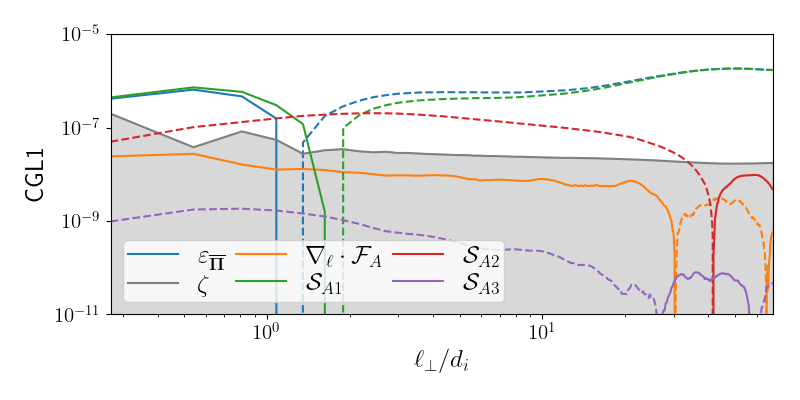
\includegraphics[width=0.9\linewidth,trim=0cm 0cm 0cm 0.5cm, clip=true]{./Mainmatter/Part_3/images_ch3/CGL1_compa_cgl}
 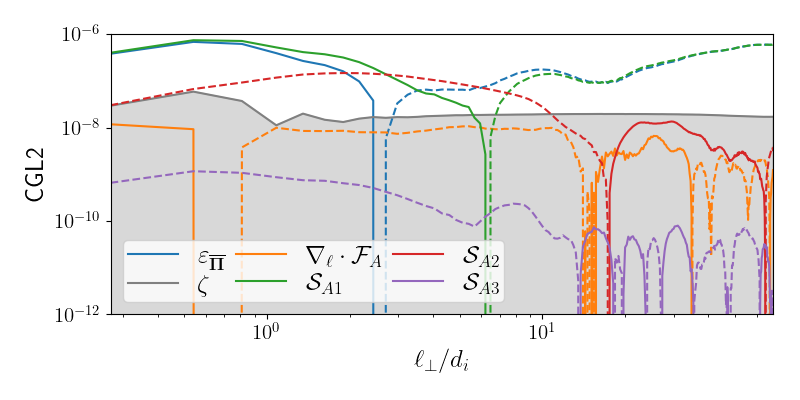
\includegraphics[width=0.9\linewidth,trim=0cm 0cm 0cm 0.5cm, clip=true]{./Mainmatter/Part_3/images_ch3/CGL2_compa_cgl}
  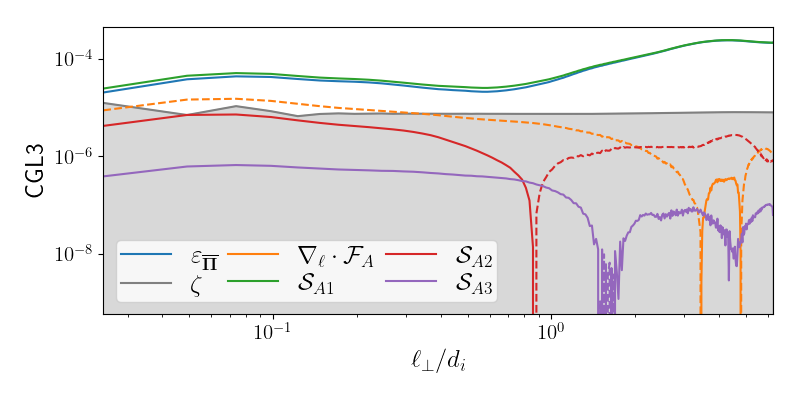
\includegraphics[width=0.9\linewidth,trim=0cm 0cm 0cm 0.5cm, clip=true]{./Mainmatter/Part_3/images_ch3/CGL3_compa_cgl}
 \cprotect\caption{Simu : CGL1 (haut), CGL2 (milieu) et  CGL3 (bas). Représentation \cacro{1D} en fonction de \ensuremath{\ell_{\perp}} du détail de \ensuremath{\varepsilon_{\overline{\boldsymbol{\Pi}}}} (bleu). Orange : \ensuremath{\nabla_{\boldsymbol{\ell}} \cdot \boldsymbol{\mathcal{F}_A}}. Vert : \ensuremath{\mathcal{S}_{A1}}. Rouge : \ensuremath{\mathcal{S}_{A2}}. Violet : \ensuremath{\mathcal{S}_{A3}}. Gris : niveau d'erreur \ensuremath{\zeta}. Les termes présents dans la zone grise délimitée par \ensuremath{\zeta} sont supposés négligeables. }
 \label{fig:detail_simu_CGL1-2}
 \end{figure}
 
 Sur la \figref{fig:detail_simu_CGL1-2}, est indiqué le détail de $\varepsilon_{\overline{\boldsymbol{\Pi}}}$ (bleu). On remarque que sont comportement est dominé par $\mathcal{S}_{A1}$ tandis que $\nabla_{\boldsymbol{\ell}} \cdot \boldsymbol{\mathcal{F}_A}$ et $\mathcal{S}_{A2}$ fluctuent autour de $\zeta$. Ils peuvent légèrement influencer $\varepsilon_{\overline{\boldsymbol{\Pi}}}$ lorsque $\mathcal{S}_{A1}$ s'affaiblit pour changer de signe, comme on peut le voir sur les résultats de CGL1 et CGL2. $\mathcal{S}_{A3}$ est, quant-à-lui, généralement négligeable. La contribution de l'anisotropie de pression et son comportement est donc principalement portée par le terme source qui survit dans la limite incompressible. Cela concorde avec la quasi-incompressibilité des simulations : l'écart-type de la densité est entre $\SI{2}{\%}$ (CGL1 et CGL2) et $\SI{8}{\%}$ (CGL3) de la moyenne. $\mathcal{S}_{A1}$ et $\varepsilon_{\overline{\boldsymbol{\Pi}}}$ doivent donc se comporter en accord avec la limite quasi-incompressible \eqref{eq:turb_cpinc_gyr1} obtenue dans le Chapitre \ref{ch-22} : 
 \begin{equation}
     \varepsilon_{\overline{\boldsymbol{\Pi}}} \simeq \mathcal{S}_{A1} \simeq \frac{\beta_0}{4}  \left< \delta \left(\left(p_{\parallel i } - p_{\perp i }\right)\left( \boldsymbol{b} \boldsymbol{b} - \frac{1}{3}  \overline{\boldsymbol{I}} \right) \right):\delta \left(\nabla \boldsymbol{v} \right)\right>
 \end{equation}
 Comprendre le comportement de ce terme est complexe puisqu'il dépend des fluctuations de la direction du champ magnétique $\boldsymbol{b}$ pondérées par l'anisotropie de la pression et distribuées sur les variations du gradient de la vitesse. $p_{\parallel i } - p_{\perp i }$ portant l'influence de l'anisotropie de pression de ce terme sur la loi exacte et pouvant s'écrire $1-a_{pi}$, on s'est intéressé au comportement statistique de $a_{pi}$. On remarque que seule la direction du champ magnétique influe sur ce terme et non son amplitude.
 
 Ces résultats sont retrouvés dans les simulations qui seront étudiées par la suite (voir Annexe \ref{an:Pi}).
 
 \subsection{Comportement statistique des pressions}
 
 La \tabref{tab:stat_CGL} résume la statistique (moyenne $\pm$ écart-type) des valeurs de la densité, de l'anisotropie de pression ionique $a_{pi} = \frac{p_{\perp i}}{p_{\parallel i}}$, et du paramètre $\beta_{\parallel} = \frac{p_{\parallel i}}{p_{m}}$ pour chaque simulation. Sur la figure \figref{fig:diag_simu_CGL}, est tracée la dispersion en fonction de $a_{pi}$ et $\beta_{\parallel}$, des simulations. Ces histogrammes \sacro{2D} prennent la forme de trois courbes de niveau formant des ovales concentriques. Le plus large contient tous les couples $\{\beta_{\parallel};a_{pi}\}$ existant dans la simulation, l'intermédiaire et le plus petit sont associés à des pourcentages du maximum de l'histogramme : $\SI{50}{\%}$ et $\SI{99}{\%}$. Sur cette figure, les critères des instabilités miroir et firehose ainsi que l'horizontale $a_{pi} =  1$ sont aussi affichés. Le critère firehose est le critère calculé dans le chapitre \ref{ch-21}, sa position sera affectée par l'effet \cacro{Hall}. Le critère miroir prend en compte la présence de la pression électronique isotherme $p_e = \rho$ et est paramétrisé par l'équation \eqref{eq:crit_miroir_elec}. Les simulations que l'on étudie ici sont données en 
 gris (CGL1), bleu (CGL2) et orange (CGL3) et correspondent aux première, deuxième et quatrième lignes du tableau. 
  \begin{table}[!ht]
 \begin{center}
 \begin{tabular}{ c|c|c|c } 
 Name & $\rho$ & $a_{pi}$  & $\beta_{\parallel}$\\
 \hline
 CGL1 & $\num{1}\pm \num{0.02}$ & $\num{1.1}\pm \num{0.1}$ & $\num{0.9}\pm \num{0.1}$ \\
 CGL2 & $\num{1}\pm \num{0.02}$ & $\num{1.1}\pm \num{0.1}$ & $\num{0.9}\pm \num{0.1}$   \\
 CGL3B & $\num{1}\pm \num{0.04}$ & $\num{1.3}\pm \num{0.3}$ & $\num{0.8}\pm \num{0.2}$   \\
 CGL3 & $\num{1}\pm \num{0.08}$ & $\num{2.2}\pm \num{0.5}$ & $\num{0.6}\pm \num{0.3}$  \\
 CGL5 & $\num{1}\pm \num{0.02}$ & $\num{2.1}\pm \num{0.1}$ & $\num{0.6}\pm \num{0.1}$  \\
 CGL6 & $\num{1}\pm \num{0.02}$ & $\num{3.97}\pm \num{0.5}$ & $\num{1.01}\pm \num{0.2}$  \\
 \end{tabular}
 \caption{Moyenne et écart-type de la densité, du taux d'anisotropie ionique $a_{pi} = \frac{p_{\perp i}}{p_{\parallel i}}$ et du paramètre $\beta_{\parallel} = \frac{p_{\parallel i}}{p_{m}}$ pour chaque simulation, à la date $t$. }\label{tab:stat_CGL}
 \end{center}
 \end{table}
 \begin{figure}[!ht]
  \centering
 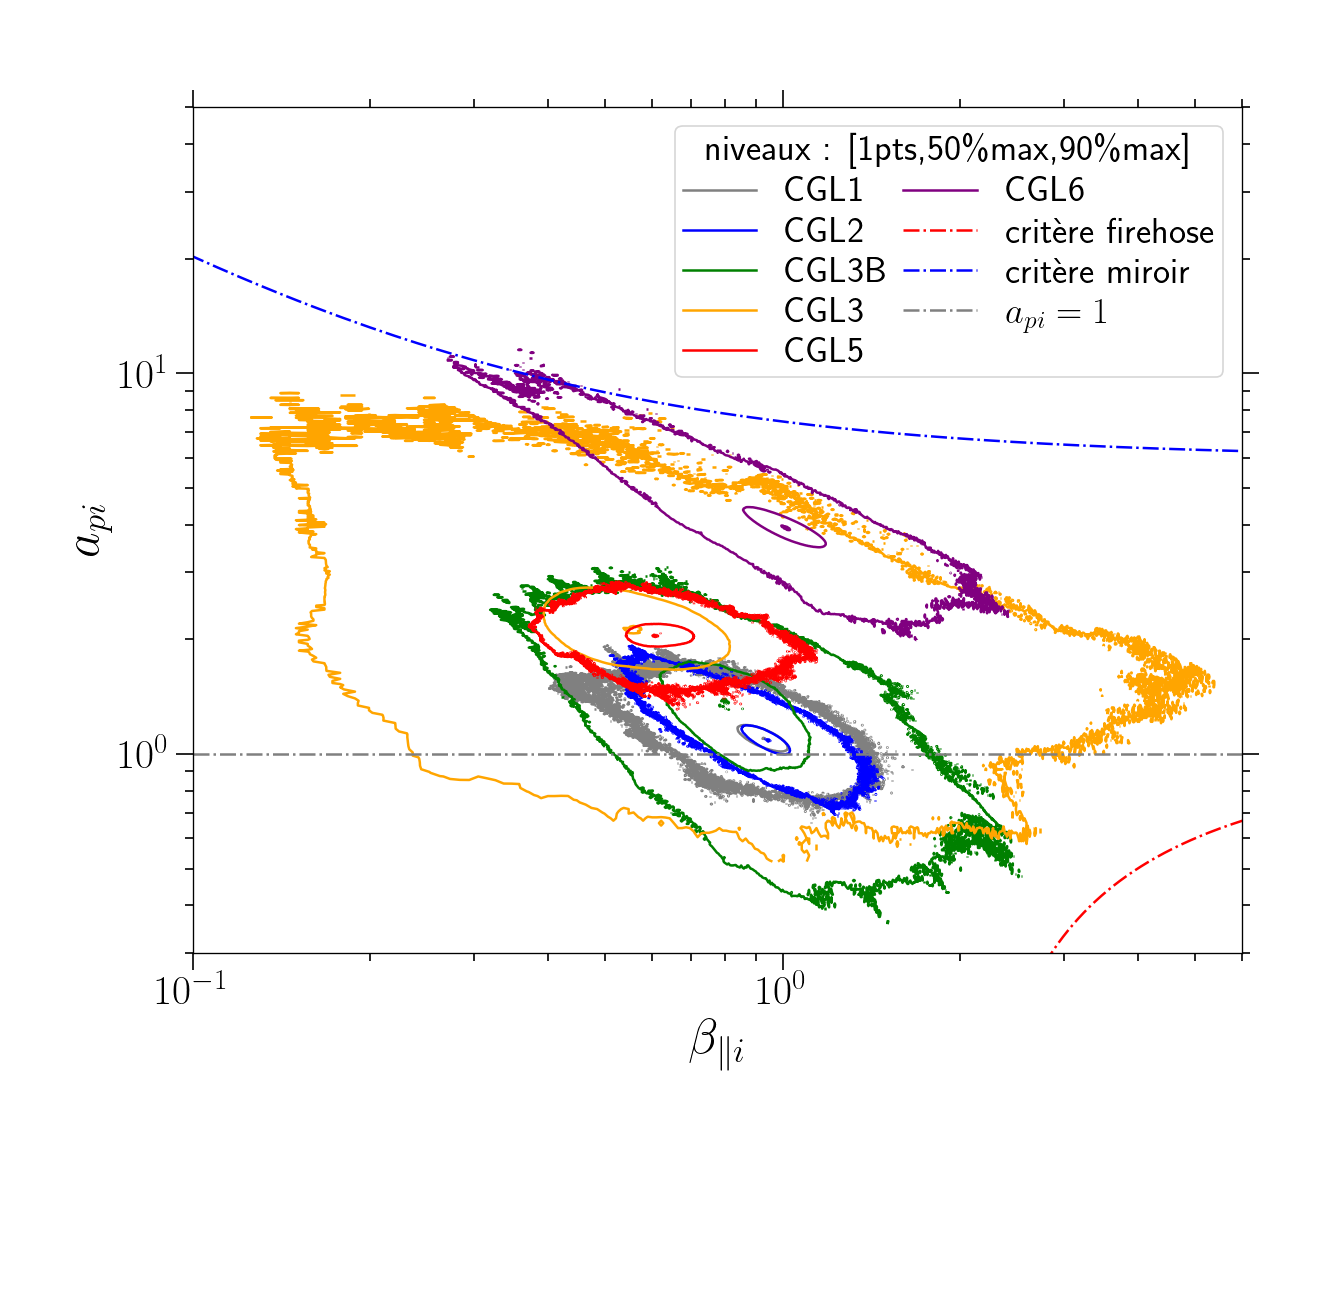
\includegraphics[width=0.8\linewidth,trim=1cm 7cm 2cm 1cm, clip=true]{./Mainmatter/Part_3/images_ch3/diag_apbeta}
 \cprotect\caption{Diagramme \ensuremath{a_{pi}-\beta_{\parallel}} contenant l'histogramme \sacro{2D} des simulations sous la forme de courbes de niveau centrées sur le couple moyen. Le critère miroir est paramétrisé par l'équation \eqref{eq:crit_miroir_elec} qui prend en compte les électrons isothermes. Le critère firehose est le critère \cacro{CGL} calculé dans le Chapitre \ref{ch-21}. }
 \label{fig:diag_simu_CGL}
 \end{figure} 
 
 On remarque que les trois simulations se sont écartées de leurs valeurs d'initialisation, $a_{piI} = 1$ et $\beta_{\parallel I} = 1$. $ \mathcal{S}_{A1}$ ne dépendant pas de $p_m$, on ne s'est pas attardé sur $\beta_{\parallel} = 1$.  Les distributions de CGL1 et de CGL2 sont quasiment identiques et très proches des valeurs initiales. CGL3 s'est quant-à-elle bien décalée et montre une moyenne $a_{pi0}\sim 2$, sa distribution est aussi beaucoup plus large avec quelques points proches du critère miroir. L'augmentation de la pression a lieu dès les premiers temps de la simulation puis reste stable. La raison d'un tel comportement est encore sujette à question : notre conjecture est qu'il est dû à l'énergie présente dans CGL3. Cette dernière est en effet forcée avec des ondes plus intenses et telle que l'énergie dans le système soit trois fois supérieure à celle dans CGL1 ou CGL2 (voir resp. $A_f$ et $E_{sup}$). Entre les points proches du critère miroir et l'augmentation de la moyenne et de l'écart-type de $a_{pi}$, beaucoup d'éléments pourraient être à l'origine de la différence de comportement de la contribution anisotrope. Ces résultats motivent d'autant plus l'obtention de nouvelles simulations. 
 
 \section{De nouvelles simulations}\label{sec-333}
 
 Trois nouvelles simulations ont été utilisées : CGL3B, CGL5 et CGL6. CGL5 et CGL6 ont été conçues et lancées pour répondre à certaines de nos questions. Comme indiqué dans le Chapitre \ref{ch-31}, obtenir des résultats de simulation valables pour une étude de turbulence prend du temps, c'est-à-dire plusieurs mois en comptant l'ajustement des paramètres d'hyperdissipation et, sachant qu'à chaque augmentation de la résolution, le temps de calcul était au moins multiplié par huit. Ainsi, d'une semaine de calcul pour faire converger le spectre associé à une résolution $258^2\times 512$, on passe à un ou deux mois pour $512^2 \times 1024$. Par conséquent, les résultats présentés ici sont récents et leur interprétation est encore en cours. 
 
 \subsection{Moins d'énergie que CGL3 : CGL3B}
 \begin{figure}[!ht]
  \centering
  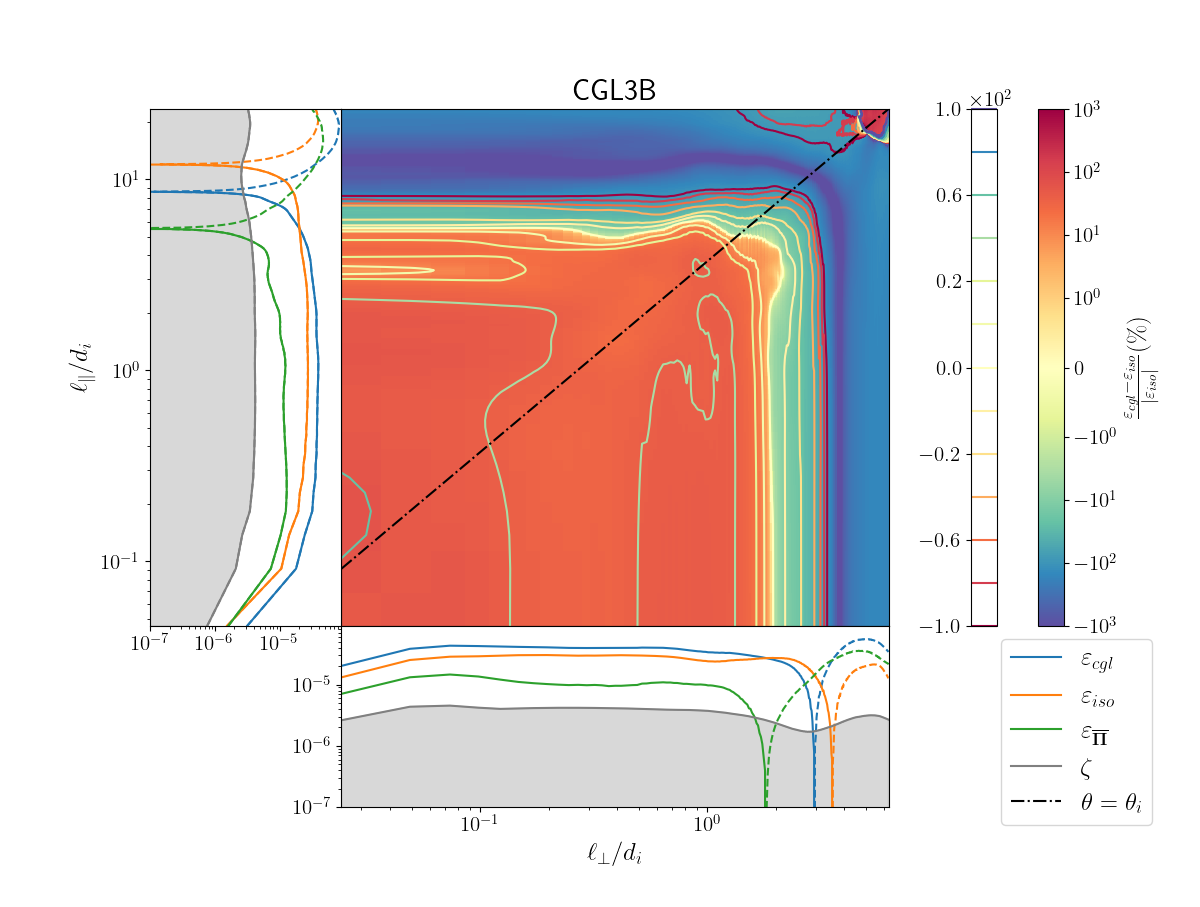
\includegraphics[width=0.95\linewidth,trim=1cm 1cm 0cm 2cm, clip=true]{./Mainmatter/Part_3/images_ch3/CGL3B_panel_isocgl_percent}
 %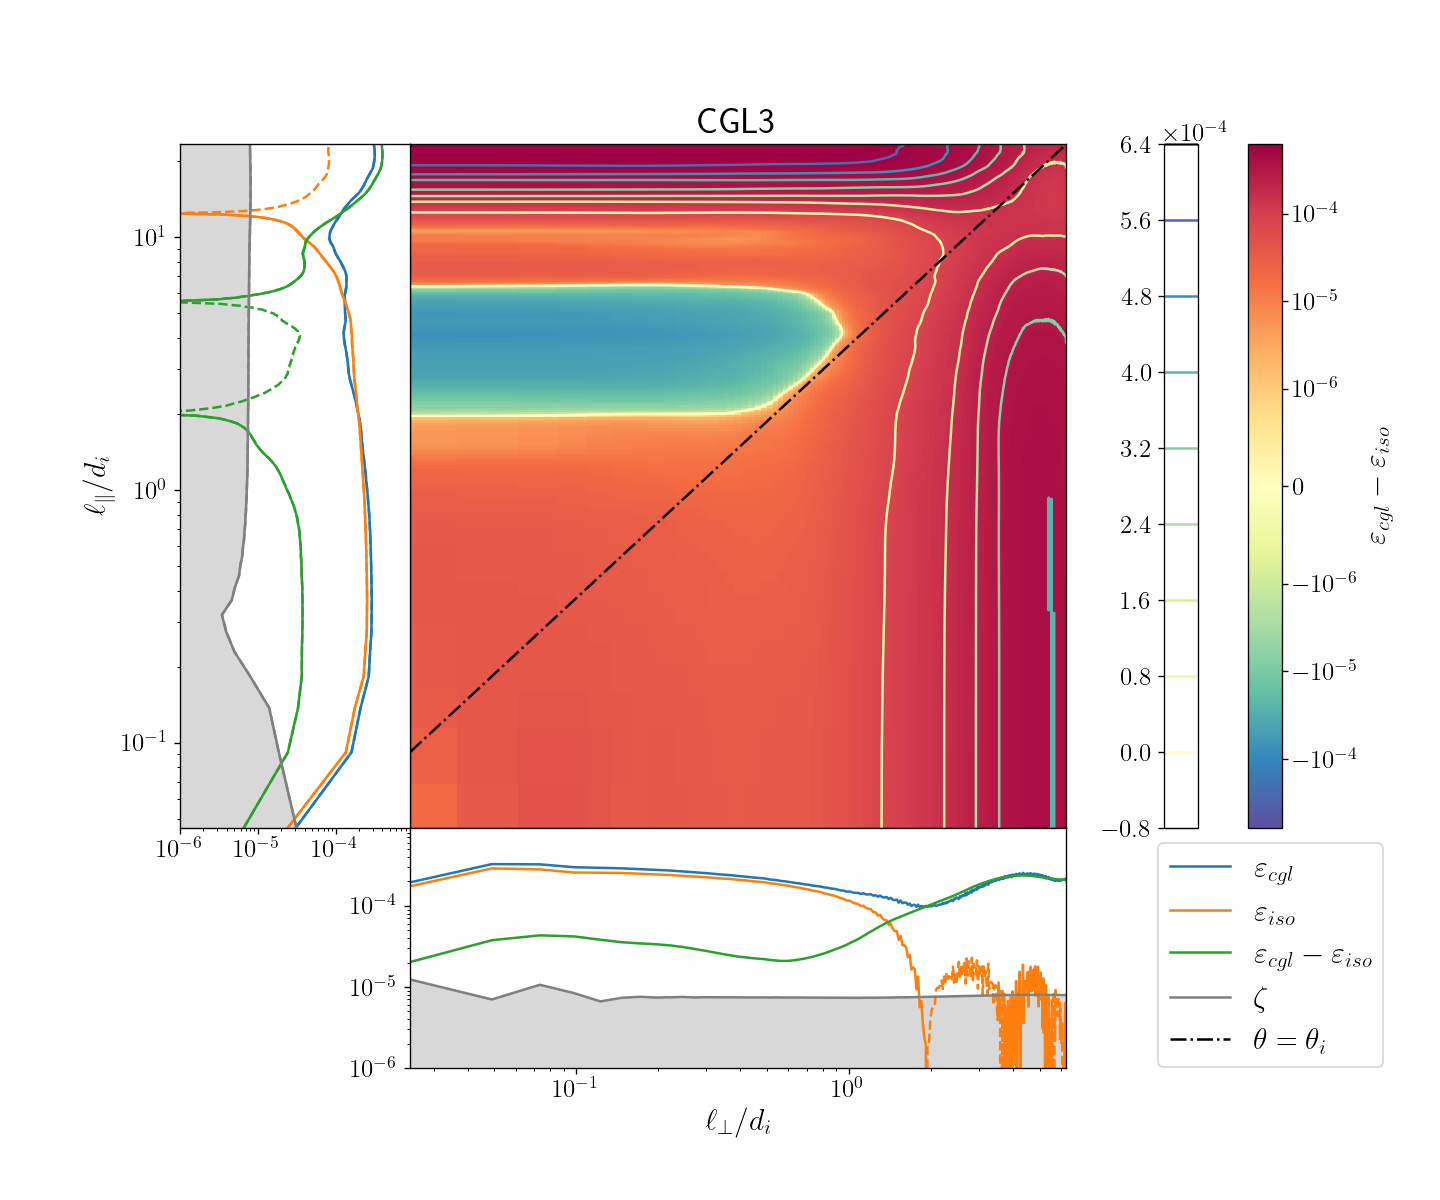
\includegraphics[width=0.95\linewidth,trim=0cm 2cm 0cm 3.5cm, clip=true]{./Part_3/images_ch3/CGL3_panel_isocgl}
 \cprotect\caption{Simu : CGL3B. Représentation \sacro{2D} en fonction de \ensuremath{\ell_{\perp}} et \ensuremath{\ell_{\parallel}} de \ensuremath{\varepsilon_{cgl}-\varepsilon_{iso}} par rapport à \ensuremath{|\varepsilon_{iso}|} en \ensuremath{\%}, entourée des représentations \cacro{1D} en fonction de \ensuremath{\ell_{\perp}} (bas) et \ensuremath{\ell_{\parallel}} (gauche) de \ensuremath{\varepsilon_{iso}} (orange), \ensuremath{\varepsilon_{cgl}} (bleu), \ensuremath{\varepsilon_{\overline{\boldsymbol{\Pi}}}} (vert) et \ensuremath{\zeta} (gris). }
 \label{fig:trip_CGL3B}
 \end{figure}
 Tout d'abord, CGL3B est une version moins énergétique de CGL3. La gamme d'échelle est donc la même, seul le forçage et par conséquent la dissipation sont affaiblis. Cette simulation est, elle aussi, initialisée telle que $a_{piI} = 1$. Sur le diagramme de la \figref{fig:diag_simu_CGL}, elle est indiquée en vert : sa moyenne, $a_{pi0} \sim 1.5$,  est entre celle de CGL2 et CGL3, et sa distribution inclue celle de CGL2 mais est moins étalée que celle de CGL3. On s'attend donc à voir les différences les plus importantes entre les résultats de l'étude des lois exactes de CGL2 et de CGL3 s'atténuer si $a_{pi}$ a de l'importance dans l'expression de la correction anisotrope.  Le triptyque fait l'objet de la \figref{fig:trip_CGL3B}. %Les contributions purement compressibles de $\varepsilon_{\overline{\boldsymbol{\Pi}}}$ étant ici aussi négligeable, on ne donnera pas son détail.
 
 À première vue, en regardant la représentation \sacro{2D}, on sait que l'on a un comportement similaire à CGL2. Le croisement entre $\varepsilon_{cgl}$ et $\varepsilon_{iso}$ dû au changement de signe de $\varepsilon_{\overline{\boldsymbol{\Pi}}}$ est toujours présent dans la zone \cacro{MHD}. Comme pour CGL3, cette zone est aussi la zone de forçage. Dans cette zone, on remarque une augmentation de la contribution venant dominer $\varepsilon_{iso}$. Si ces deux éléments ne sont pas des artefacts dus à l'oscillation du forçage, cela signifie que, contrairement à CGL3 et similairement à CGL1 et CGL2, le changement de signe a lieu avant l'augmentation, et cela tend à indiquer que l'augmentation présente dans CGL3 est intrinsèque à la zone de forçage.
 
 La zone inertielle est située entre $\ell_{\perp} \in [\num{0.1};\num{2}]$ et $\ell_{\parallel} \in [\num{0.2};\num{4}]$. Cette fois-ci, $\varepsilon_{\overline{\boldsymbol{\Pi}}}$ contribue à $\SI{30}{\%}$ de $\varepsilon_{iso}$. On a donc un facteur 3 par rapport aux $\SI{10}{\%}$ relevés pour les autres simulations. Ce résultat, significatif, indique que l'anisotropie de pression semble affecter la zone inertielle mais interpelle aussi car, pour une simulation que tout semble placer entre CGL2 et CGL3, l'effet de l'anisotropie de pression sur la zone inertielle en est éloigné. La source d'un tel comportement est encore en cours de discussion. 
  
 % \begin{figure}[!ht]
 %  \centering
 % 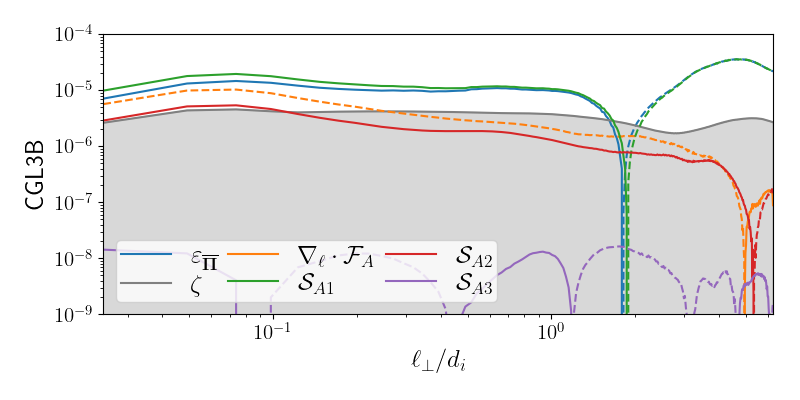
\includegraphics[width=1\linewidth,trim=0cm 1cm 0cm 1cm, clip=true]{./Part_3/images_ch3/CGL3B_compa_cgl}
 % % \includegraphics[width=1\linewidth,trim=0cm 1cm 0cm 1cm, clip=true]{./Part_3/images_ch3/CGL3_compa_cgl}
% \cprotect\caption{Représentation \acs{1D} en fonction de $\ell_{\perp}$ du détail de $\varepsilon_{\overline{\boldsymbol{\Pi}}}$ (bleu). Orange : $\nabla_{\boldsymbol{\ell}} \cdot \boldsymbol{\mathcal{F}_A}$. Vert : $\mathcal{S}_{A1}$. Rouge : $\mathcal{S}_{A2}$. Violet : $\mathcal{S}_{A3}$. Gris : niveau d'erreur $\zeta$. Les termes présents dans la zone grise délimitée par $\zeta$ sont supposés négligeables. Simu : CGL3B. }
% \label{fig:detail_simu_CGL3B}
% \end{figure}

\subsection{Une gamme d'échelle intermédiaire : CGL5}
\begin{figure}[!ht]
 \centering
 \includegraphics[width=0.95\linewidth,trim=1cm 1cm 0cm 2cm, clip=true]{./Mainmatter/Part_3/images_ch3/CGL5_panel_isocgl_percent}
 \cprotect\caption{Simu : CGL5. Représentation \sacro{2D} en fonction de \ensuremath{\ell_{\perp}} et \ensuremath{\ell_{\parallel}} de \ensuremath{\varepsilon_{cgl}-\varepsilon_{iso}} par rapport à \ensuremath{|\varepsilon_{iso}|} en \ensuremath{\%}, entourée des représentations \cacro{1D} en fonction de \ensuremath{\ell_{\perp}} (bas) et \ensuremath{\ell_{\parallel}} (gauche) de \ensuremath{\varepsilon_{iso}} (orange), \ensuremath{\varepsilon_{cgl}} (bleu), \ensuremath{\varepsilon_{\overline{\boldsymbol{\Pi}}}} (vert) et \ensuremath{\zeta} (gris). }
\label{fig:trip_CGL5}
\end{figure}

 La gamme d'échelles accessible via CGL5 est située entre celles de CGL2 et celles de CGL3 afin de couvrir la transition entre la zone \cacro{MHD} et la zone \cacro{Hall}, tout en gardant éloignées les échelles impactées par l'injection d'énergie. %Sur la \tabref{tab:stat_CGL}, on voit que sa compression est similaire à celle de CGL2, les termes purement compressibles seront encore une fois négligeables.
 L'écart-type de sa distribution est aussi de l'ordre de celui de CGL2, tout comme son étalement dans le diagramme de la \figref{fig:diag_simu_CGL}, mais sa position centrale y est plus proche de celle de CGL3. Le comportement observé pourrait donc être en faveur de la conjecture d'un impact de la moyenne de $a_{pi}$ ou de celle d'un impact des fluctuations sur la contribution du taux de cascade dépendant de l'anisotropie de pression. 
 
 % \begin{figure}[!ht]
 %  \centering
 %  \includegraphics[width=1\linewidth,trim=0cm 1cm 0cm 1cm, clip=true]{./Part_3/images_ch3/CGL5_compa_cgl}
 % \cprotect\caption{Simu : CGL5. Représentation 1D en fonction de $\ell_{\perp}$ du détail de $\varepsilon_{\overline{\boldsymbol{\Pi}}}$ (bleu). Orange : $\nabla_{\boldsymbol{\ell}} \cdot \boldsymbol{\mathcal{F}_A}$. Vert : $\mathcal{S}_{A1}$. Rouge : $\mathcal{S}_{A2}$. Violet : $\mathcal{S}_{A3}$. Gris : niveau d'erreur $\zeta$. Les termes présents dans la zone grise délimitée par $\zeta$ sont supposés négligeables. }
 % \label{fig:detail_simu_CGL5}
 % \end{figure}
 
 Sur le triptyque obtenu pour CGL5 (\figref{fig:trip_CGL5}), on observe un comportement similaire à celui de CGL3. Dans la zone inertielle ($\ell_{\perp} \in [\num{0.3};\num{5}]$\footnote{La taille de la zone inertielle perpendiculaire dans la représentation \cacro{1D} de la \figref{fig:trip_CGL5} est réduite à cause de la \og bulle \fg{} négative parallèle et du filtrage angulaire. La valeur maximale est donc estimée à partir de la représentation \sacro{2D}.}), la contribution de $\varepsilon_{\overline{\boldsymbol{\Pi}}}$ est de l'ordre de $\SI{10}{\%}$ de $\varepsilon_{iso}$. Ces résultats confirment que le comportement de CGL3 n'est pas un cas particulier et se placent en faveur de la moyenne de $a_{pi}$ plutôt que de ses fluctuations. De plus, l'augmentation à grande échelle visible pour CGL3 s'est déportée avec le forçage, confirmant qu'elle est intrinsèque à la zone d'injection de l'énergie dans la cascade.  


\subsection{Une initialisation anisotrope $a_{piI} = 4$ : CGL6}
\begin{figure}[!ht]
 \centering
\includegraphics[width=0.95\linewidth,trim=1cm 1cm 0cm 2cm, clip=true]{./Mainmatter/Part_3/images_ch3/CGL6_panel_isocgl_percent}
\cprotect\caption{Simu : CGL6. Représentation \sacro{2D} en fonction de \ensuremath{\ell_{\perp}} et \ensuremath{\ell_{\parallel}} de \ensuremath{\varepsilon_{cgl}-\varepsilon_{iso}} par rapport à \ensuremath{|\varepsilon_{iso}|} en \ensuremath{\%}, entourée des représentations \cacro{1D} en fonction de \ensuremath{\ell_{\perp}} (bas) et \ensuremath{\ell_{\parallel}} (gauche) de \ensuremath{\varepsilon_{iso}} (orange), \ensuremath{\varepsilon_{cgl}} (bleu), \ensuremath{\varepsilon_{\overline{\boldsymbol{\Pi}}}} (vert) et \ensuremath{\zeta} (gris). }
\label{fig:trip_CGL6}
\end{figure}
La dernière simulation lancée est CGL6. Elle est basée sur CGL5 mais initialisée avec une pression anisotrope : $a_{piI} = 4 $. Le but de cette simulation est double :
\begin{itemize}
    \item vérifier si l'un des comportements observés précédemment pour notre correction se maintient lorsque la simulation est initialisée anisotropiquement,
    \item se rapprocher du critère miroir.
\end{itemize}
Des valeurs de $a_{piI}$ plus importantes ont été testées, mais seule la simulation avec $a_{piI} = 4 $ a pu être numériquement stabilisée. 

 Comme on peut le voir sur la \tabref{tab:stat_CGL} et sur la \figref{fig:diag_simu_CGL} (violet), cette simulation se maintient au niveau de $a_{piI}$. En fait, c'est la seule simulation montrant un $a_{pi0}$ aussi proche de sa condition initiale, l'écart n'étant que de $\SI{3}{\%}$. Pour ce qui est du but de se rapprocher du critère miroir, le diagramme nous indique que quelques points de CGL6 sont situés au-dessus du critère miroir. Le développement d'instabilité miroir semble donc permis dans cette simulation. 
 
 Sur la \figref{fig:trip_CGL6},  $\varepsilon_{\overline{\boldsymbol{\Pi}}}$ est entièrement positif. Son niveau est de l'ordre de $\SI{70}{\%}$ de $\varepsilon_{iso}$ aux échelles inertielles, c'est-à-dire pour $\ell_{\perp} \in [\num{0.3};\num{1}]$. Il a donc bien augmenté par comparaison avec les $\SI{10}{\%}$ et $\SI{30}{\%}$ précédents. Par comparaison avec CGL5, la gamme d'échelles inertielles est réduite par l'augmentation de $\varepsilon_{\overline{\boldsymbol{\Pi}}}$ qui est plus étalée. %Les termes purement compressibles sont toujours de l'ordre de l'erreur numérique.


% \begin{figure}[!ht]
%  \centering
% \includegraphics[width=1\linewidth,trim=0cm 1cm 0cm 1cm, clip=true]{./Part_3/images_ch3/CGL6_compa_cgl}
% \cprotect\caption{Simu : CGL6. Représentation 1D en fonction de $\ell_{\perp}$ du détail de $\varepsilon_{\overline{\boldsymbol{\Pi}}}$ (bleu). Orange : $\nabla_{\boldsymbol{\ell}} \cdot \boldsymbol{\mathcal{F}_A}$. Vert : $\mathcal{S}_{A1}$. Rouge : $\mathcal{S}_{A2}$. Violet : $\mathcal{S}_{A3}$. Gris : niveau d'erreur $\zeta$. Les termes présents dans la zone grise délimitée par $\zeta$ sont supposés négligeables. De haut en bas : CGL3, CGL5 et CGL6. }
% \label{fig:detail_simu_CGL6}
% \end{figure}

\section{Synthèse de l'étude préliminaire des simulations CGL-MHD-Hall-\ensuremath{\nabla P_e}}
\label{synth-33}

{\bf Les résultats présentés dans ce chapitre nous permettent de valider numériquement l'apport de la correction dépendant de l'anisotropie de pression dans le cas quasi-incompressible. Ils nous confirment aussi que, dans un cadre quasi-incompressible, le terme dominant est celui qui vient former la correction de \cacro{PP98} dans la limite incompressible gyrotrope (Chapitre \ref{ch-22}).} Cela implique que la première correction devant être appliquée dans un plasma quasi-incompressible tel que le vent solaire n'est peut-être pas la compression mais plutôt l'anisotropie de pression. Cette étude numérique n'est cependant qu'à un stade préliminaire. En effet, nous n'avons pas encore convergé sur l'interprétation d'un certain nombre d'éléments et, comme nous venons de le voir, elle soulève un nombre important de questions.


\begin{figure}[!ht]
 \centering
 \includegraphics[width=0.9\linewidth,trim=3cm 1cm 5cm 1cm, clip=true]{./Mainmatter/Part_3/images_ch3/scattersimu}
\cprotect\caption{Résumé de l'étude préliminaire sur l'effet de l'anisotropie de pression sur le taux de transfert non linéaire en fonction de \ensuremath{a_{pi0}} (première colonne) et de \ensuremath{\text{std}(a_p)} (deuxième colonne). Chaque simulation est associée à une couleur (même association que pour la \figref{fig:diag_simu_CGL}). (A) : histogramme de \ensuremath{a_p}, CGL1 y est confondu avec CGL2. (B) et (C) : apport de la contribution de la pression anisotrope. (D) et (E) : impact de l'augmentation dans la zone de forçage de la contribution anisotrope sur le niveau du taux de transfert total mesuré dans la zone inertielle.}
\label{fig:scattersimu}
\end{figure}
 
 On propose une synthèse à travers la \figref{fig:scattersimu}. Sur le graphique $(A)$ sont repris les histogrammes de $a_{pi}$, (CGL1 y est confondu avec CGL2). Les simulations sont ordonnées par couleur et comportement : les simulations présentant un changement de signe sont en gris (CGL1), bleu (CGL2) et vert (CGL3B). Celles  montrant un signe quasiment isotrope à l'exception d'une \og bulle \fg{} dans la direction parallèle sont en jaune (CGL3) et rouge (CGL5). La dernière simulation, initialisée avec $a_{piI}  = 4$, montrant une contribution anisotrope entièrement positive, est donnée en violet (CGL6). Deux paramètres liés à la distribution de $a_{pi}$ ont été abordés : la moyenne $a_{pi0}$ (graphique $(B)$ et $(C)$) et l'écart-type $\text{std}(a_{pi})$ (graphique $(D)$ et $(E)$). En fonction de $a_{pi0}$, les simulations se comportant similairement restent groupées, contrairement à $\text{std}(a_{pi})$. $a_{pi0}$ semble donc être un meilleur paramètre que $\text{std}(a_{pi})$. Sur le graphique $(B)$, sont placées les estimations de la contribution anisotrope au taux de cascade dans la zone inertielle. On y observe que CGL3B et CGL6 s'écartent du résultat des autres simulations. Ce résultat est inattendu pour CGL3B (ou CGL3 et CGL5). Si $a_{pi0}$ est bien le paramètre important dans l'impact des anisotropies de pression sur la cascade et que CGL3B est bien valable et n'est pas une exception, alors il pourrait exister un processus qui viendrait inverser, pour quelques $a_{pi0}$, la tendance croissante de la contribution anisotrope dans la zone inertielle. Pour ce qui est du rapport entre le taux de transfert non linéaire estimé dans la zone de forçage et le taux de cascade inertielle (graphique (D)), il semble globalement croitre en fonction de $a_{pi0}$. Il serait intéressant d'y évaluer plus précisément l'impact de l'injection d'énergie afin de vérifier si un autre processus intervient. 
 
 Ces graphiques, contenant un nombre limité de points lié au nombre de simulations à disposition, ne sont, bien évidemment, que des outils de spéculation, synthétisant cette étude préliminaire et permettant de dégager des tendances pour lesquelles l'analyse pourra être approfondie.




% \section{Etude de spectre } \label{sec-334}

% Sachant que le forçage se fait avec des modes aléatoires de fréquences proches de celle du mode d'Alfvén et que des études telles celle de \cite{brodiano_spatiotemporal_2021} ont relié le choix de forçage aux ondes dominant la simulation, observer une cascade développée par des ondes d'Alfvén dans nos simulations serait tout à fait réaliste. Si l'on regarde les spectres de champs magnétiques parallèle et perpendiculaire de CGL2 par exemple (\figref{fig:spectre}), on remarque que le spectre d'énergie magnétique est dominé par les fluctuations perpendiculaires au champ magnétique ambiant et on y retrouve les pentes turbulentes en $-5/3$ (zone MHD) et en $-7/3$ (zone Hall).  Un tel résultat est une signature de la nature alfvénique de la cascade turbulente. Il n'est donc pas impossible que la correction d'anisotropie de pression soit dominé par la correction firehose. 
% \begin{figure}[!ht]
%  \centering
% \includegraphics[width=0.95\linewidth,trim=0cm 0cm 0cm 0cm, clip=true]{./Part_3/images_ch3/CGL2_spectre}
% \cprotect\caption{Simu : CGL2. Spectre d'énergie magnétique perpendiculaire et parallèle en fonction de $k_{\perp}d_i$}
% \label{fig:spectre}
% \end{figure}

% Sur le spectre des fluctuations perpendiculaires, on peut remarquer une bosse en $k_{\perp}d_i = 0.3$, cela correspondrait à $\ell_{\perp}/d_i = 21 $. Si l'on regarde sur le triptyque associé à CGL2 (\figref{fig:trip_CGL1-2}), on remarque que cette échelle correspond au début de l'augmentation de $\varepsilon_{\overline{\boldsymbol{\Pi}}}$. 

% Les spectres de CGL5 et CGL6 sont plus complexes à analyser, la contribution des fluctuations parallèles au spectre total prend de l'importance dans la zone Hall, comme on peut le voir pour sur la \figref{fig:spectre_CGL6}. Serait la signature d'une cascade d'ondes magnétosonores ?
% \begin{figure}[!ht]
%  \centering
% \includegraphics[width=0.95\linewidth,trim=0cm 0cm 0cm 0cm, clip=true]{./Part_3/images_ch3/CGL6_spectre}
% \cprotect\caption{Simu : CGL6. Spectre d'énergie magnétique perpendiculaire et parallèle en fonction de $k_{\perp}d_i$. Le spectre est compensé par la pente $-7/3$ attendue dans la zone inertielle Hall.}
% \label{fig:spectre_CGL6}
% \end{figure}

\chapter{Vers l'étude des simulations Landau-fluides}
\renewcommand\partie{\Partie\ Chapitre \thechapter}
\label{ch-34}

\bigskip
\minitoc  

\cite{ferrand_fluid_2021} ont aussi utilisé des simulations du modèle \acs{LFHPe} prenant en compte un flux de chaleur $\overline{\overline{\boldsymbol{q}}}$ gyrotrope obtenu grâce à une fermeture Landau-fluide présente dans le code utilisé dans cette partie. Il s'est avéré que ces simulations prennent aussi en compte un tenseur de pression électronique de type gyrotrope.
Ces simulations corrigeant les critères d'instabilités tel que le critère miroir afin de refléter le comportement linéaire cinétique, elles pourraient par la suite nous aider à étendre nos interprétations vers les processus cinétiques. 

Dans ce chapitre, nous décrivons les spécificités du modèle implémenté et la loi exacte complète associée. Une première application, préliminaire, à deux simulations, semblent montrer des résultats paradoxaux qui nécessiteront une étude plus fine avant d'en extraire un début d'interprétations. 


\section{Modèle simulé et loi exacte}
\label{sec-341}

Dans ce deuxième lot de simulations, les ions et les électrons sont décrits avec un tenseur de pression gyrotrope. La fermeture utilisée est une fermeture Landau-fluide. Cette fermeture nous rapproche d'un modèle cinétique en prenant en compte l'amortissement Landau linéaire (phénomène cinétique) dans le modèle fluide. Cette correction étant basée sur la relation de dispersion cinétique, les critères d'instabilité seront aussi corrigés pour correspondre aux critères cinétiques. La gyrotropie des électrons impactera d'ailleurs le critère miroir. Les flux de chaleur ioniques et électroniques sont aussi supposés gyrotropes.

Les premières équations du modèle normalisé simulé sont les suivantes, en y faisant apparaître indépendamment les tenseurs de pression ionique et électronique : 
\begin{eqnarray}
\label{eq:mlf_r} \partial_t \rho + \nabla \cdot \left(\rho \boldsymbol{v}\right) &=& 0\\
\label{eq:mlf_v} \partial_t  \boldsymbol{v} + \boldsymbol{v} \cdot \nabla  \boldsymbol{v} - \frac{1}{\rho} \boldsymbol{j} \times \boldsymbol{B} + \frac{1}{\rho} \nabla \cdot \left(\overline{\boldsymbol{P_i}} + \overline{\boldsymbol{P_e}} \right)  &=& 0  \\
\label{eq:mlf_b} \partial_t \boldsymbol{B} - \nabla \times \left( \boldsymbol{v} \times \boldsymbol{B} \right) +  d_i  \nabla \times \left( \frac{1}{\rho} \boldsymbol{j}\times \boldsymbol{B} \right) &=& d_i \nabla \times \left( \frac{1}{\rho} \nabla \left(  p_e\right) \right)  \\
\label{eq:mlf_pperpi} \partial_t  p_{\perp i }  +  \nabla \cdot \left(p_{\perp i } \boldsymbol{v} \right) +  p_{\perp i }\nabla \cdot\boldsymbol{v} -  p_{\perp i } \boldsymbol{b}\boldsymbol{b} : \nabla \boldsymbol{v}  &=& - \frac{1}{2} \left( \text{Tr}(\nabla \cdot \overline{\overline{\boldsymbol{q_i}}}) - \boldsymbol{b}\boldsymbol{b} : \nabla \cdot \overline{\overline{\boldsymbol{q_i}}} \right) \nonumber \\ && \\
\label{eq:mlf_ppari} \partial_t  p_{\parallel i }  +  \nabla \cdot \left(p_{\parallel i } \boldsymbol{v} \right) +  2 p_{\parallel i }  \boldsymbol{b}\boldsymbol{b} : \nabla \boldsymbol{v}  &=&  - \boldsymbol{b}\boldsymbol{b} : \nabla \cdot \overline{\overline{\boldsymbol{q_i}}}   \\
\label{eq:mlf_pperpe} \partial_t  p_{\perp e }  +  \nabla \cdot \left(p_{\perp e } \boldsymbol{v_e} \right) +  p_{\perp e }\nabla \cdot\boldsymbol{v_e} -  p_{\perp e } \boldsymbol{b}\boldsymbol{b} : \nabla \boldsymbol{v_e}  &=&  - \frac{1}{2} \left( \text{Tr}(\nabla \cdot \overline{\overline{\boldsymbol{q_e}}}) - \boldsymbol{b}\boldsymbol{b} : \nabla \cdot \overline{\overline{\boldsymbol{q_e}}} \right) \nonumber \\ && \\
\label{eq:mlf_ppare} \partial_t  p_{\parallel e }  +  \nabla \cdot \left(p_{\parallel e } \boldsymbol{v_e} \right) +  2 p_{\parallel e }  \boldsymbol{b}\boldsymbol{b} : \nabla \boldsymbol{v_e}  &=& - \boldsymbol{b}\boldsymbol{b} : \nabla \cdot \overline{\overline{\boldsymbol{q_e}}} 
\end{eqnarray}

avec $\overline{\boldsymbol{P_{i,e}}} =  \frac{\beta_0}{2} \left(p_{\perp i,e } \overline{\boldsymbol{I}} + \left(p_{\parallel i,e } - p_{\perp i,e }\right) \boldsymbol{b} \boldsymbol{b} \right) $, les tenseurs gyrotropes de pression ionique (i) et électronique (e), $\boldsymbol{b} = \frac{\boldsymbol{B}}{|\boldsymbol{B}|}$, la direction du champ magnétique, $\frac{\beta_0}{2} $ constante provenant de la normalisation des équations, et $\boldsymbol{v_e} = \boldsymbol{v} - d_i \frac{\boldsymbol{j}}{\rho} $ la vitesse électronique. La fermeture est appliquée au niveau du quatrième moment (pour plus d'informations, voir les premières parties de \cite{passot_collisionless_2007}) présent dans les équations de $ \overline{\overline{\boldsymbol{q_i}}}$ et $ \overline{\overline{\boldsymbol{q_e}}}$. L'hypothèse de gyrotropie appliquée aux tenseurs de flux de chaleur implique (avec $s = i,e$) :  
\begin{eqnarray*}
    \boldsymbol{b}\boldsymbol{b} : \nabla \cdot \overline{\overline{\boldsymbol{q_s}}} &\simeq& \nabla \cdot (q_{\parallel s} \boldsymbol{b}) - 2 q_{\perp s} \nabla \cdot \boldsymbol{b}\\
    \frac{1}{2} \left( \text{Tr}(\nabla \cdot \overline{\overline{\boldsymbol{q_s}}}) - \boldsymbol{b}\boldsymbol{b} : \nabla \cdot \overline{\overline{\boldsymbol{q_s}}} \right)  &\simeq&  \nabla \cdot (q_{\perp s} \boldsymbol{b})  + q_{\perp s} \nabla \cdot \boldsymbol{b}
\end{eqnarray*}


L'équation d'énergie interne peut être construite à partir des équations de pression \eqref{eq:mlf_ppari}, \eqref{eq:mlf_pperpi}, \eqref{eq:mlf_ppare}, \eqref{eq:mlf_pperpe} et de la relation $\boldsymbol{v_e} = \boldsymbol{v} - d_i \frac{\boldsymbol{j}}{\rho} $  : 
\begin{eqnarray}
\label{eq:mlf_ui} \partial_t \left(\rho u\right) + \nabla \cdot \left(\rho u \boldsymbol{v} + \boldsymbol{q}\right) +   \left(\overline{\boldsymbol{P_i}} + \overline{\boldsymbol{P_e}} \right): \nabla \boldsymbol{v} &=& \frac{d_i}{2}  \nabla \cdot  \left(\text{Tr} \left(\overline{\boldsymbol{P_e}}\right)  \frac{ \boldsymbol{j}}{\rho} \right) +  d_i \overline{\boldsymbol{P_{e}}} : \nabla \left(\frac{\boldsymbol{j}}{\rho} \right)\nonumber \\ 
\end{eqnarray}
sachant que $\rho u = \frac{\beta_0}{2} \left(p_{\perp i } + \frac{1}{2}p_{\parallel i} + p_{\perp e } + \frac{1}{2}p_{\parallel e} \right) $ et avec $\boldsymbol{q} = \frac{\beta_0}{2} \left(q_{\perp i } + \frac{1}{2}q_{\parallel i} + q_{\perp e } + \frac{1}{2}q_{\parallel e} \right)  \boldsymbol{b}$. 

La loi exacte valable pour ce modèle a pour base \eqref{eq:turb_cpg_elk} à laquelle on doit ajouter la correction Hall \eqref{eq:corr_hall}, la correction dépendant de la pression électronique \eqref{eq:corr_pe} et la correction dépendant des flux de chaleur \eqref{eq:turb_ref_q}. 

Par curiosité, nous l'avons appliquée à deux simulations LF2 et LF3, pour vérifier si l'on pouvait retrouver les conclusions de \cite{ferrand_fluid_2021} à travers les termes dépendant des flux de chaleurs. 

\section{Etude préliminaire des simulations}
\label{sec-342}

Les paramètres initiaux associés à chaque simulation sont donnés dans la \tabref{tab:setups} et la \tabref{tab:setups_hd}. Et, dans la \tabref{tab:stat_LF}, sont repris quelques informations statistiques. Similairement aux simulations \acs{CGLHPe}, les fluctuations de densité  sont faibles, ces simulations sont aussi quasi-incompressibles. 
 \begin{table}[!ht]
\begin{center}
\begin{tabular}{ c|c|c|c|c|c } 
Name & $\rho$ & $a_{pi}$  & $\beta_{\parallel i }$ & $a_{pe}$  & $\beta_{\parallel e }$\\
\hline
%LF1 & $\num{1}\pm \num{0.02}$ & $\num{1.04}\pm \num{0.04}$ & $\num{0.97}\pm \num{0.06}$ & $\num{1.01}\pm \num{0.003}$ & $\num{0.99}\pm \num{0.07}$ \\
LF2 & $\num{1}\pm \num{0.01}$ & $\num{1.05}\pm \num{0.03}$ & $\num{0.97}\pm \num{0.04}$ & $\num{1.01}\pm \num{0.006}$ & $\num{0.98}\pm \num{0.05}$  \\
LF3 & $\num{1}\pm \num{0.08}$ & $\num{1.52}\pm \num{0.31}$ & $\num{0.84}\pm \num{0.30}$ & $\num{0.96}\pm \num{0.04}$ & $\num{1.10}\pm \num{0.42}$  %\\
%LF4 & $\num{1}\pm \num{0.02}$ & $\num{1.07}\pm \num{0.05}$ & $\num{0.94}\pm \num{0.07}$ & $\num{1.07}\pm \num{0.02}$ & $\num{0.92}\pm \num{0.05}$ 
\end{tabular}
\caption{Moyenne et écart-type de la densité, du taux d'anisotropie ionique $a_{pi} = \frac{p_{\perp i}}{p_{\parallel i}}$ et électronique $a_{pe} = \frac{p_{\perp e}}{p_{\parallel e}}$ et des paramètres $\beta_{\parallel i} = \frac{p_{\parallel i}}{p_{m}}$ et $\beta_{\parallel e} = \frac{p_{\parallel e}}{p_{m}}$  pour chaque simulation, à la date $t$. \label{tab:stat_LF}}
\end{center}
\end{table}
\begin{figure}[!ht]
 \centering
\includegraphics[width=1\linewidth,trim=0cm 2cm 1cm 1cm, clip=true]{./Part_3/images_ch4/diag_simu_LF}
\cprotect\caption{Diagramme $a_{pi}-\beta_{\parallel i}$ contenant l'histogramme \acs{2D} des simulations LF2 et LF3 sous la forme de courbes de niveau centrées sur le couple moyen. Les lignes discontinues correspondent aux critères d'instabilité. Rouge : le critère firehose CGL calculé dans le chapitre \ref{ch-21} et valable dans les modèles cinétique [\cite{hunana_introductory_2019}], il ne prend pas en compte l'effet \acs{Hall}. Cyan : critère miroir cinétique (sans prise en compte de la pression électronique) [\cite{hunana_introductory_2019}]. Bleu : critère miroir proposé par \cite{kuznetsov_mirror_2012}, prenant en compte les électrons gyrotropes et calculé avec $a_{pe} = 1$ et $\beta_{\parallel e } = 1$.}
\label{fig:diag_simu_LF}
\end{figure} 

Les taux d'anisotropie initialisés à $\num{1}$ sont restés proches de 1 et sont moins étalées que ceux des simulations \acs{CGLHPe} CGL2 et CGL3. LF3 montre un étalement plus important similairement à CGL3. Plus d'un tiers des points sont situés dans la zone du diagramme située du côté instable du critère miroir. Deux critères miroirs sont donnés. Le premier en cyan correspond au critère cinétique obtenue en corrigeant le facteur 6 du critère CGL [\cite{galeev_mhd_1983,ferriere_mixed_2002,hunana_introductory_2019}]. Le second, en bleu, est aussi un critère miroir cinétique mais prenant en compte l'anisotropie de pression électronique. Ce critère est dérivé dans l'article [\cite{kuznetsov_mirror_2012}]. Il est ici représenté en considérant $a_{pe} = 1$ et $\beta_{\parallel e } = 1$. 

Les simulations LF pourrait donc permettre une étude fine de l'impact des instabilités cinétiques sur la cascade turbulente. Mais, en première application de la loi exacte étendue et par curiosité, nous avons d'abord cherché à retrouver les résultats de \ac{F21}. 



\section{Premières applications de la loi exacte \acs{LFHPe}}
\label{sec-343}

Pour les simulations LF2 et LF3, l'extraction d'échantillons de temps consécutifs n'a pas encore été fait. On ne fera donc pas apparaître le niveau $\zeta$ dans les résultats qui suivent qui sont préliminaires.

L'une des questions que nous nous sommes posés est : est-ce que l'on retrouve la décroissance associée au flux de chaleur par \ac{F21} ? On a alors calculé le taux de cascade total dans LF2 et LF3 avec ($\varepsilon|\nabla \cdot \boldsymbol{q} \neq 0$) et sans ($\varepsilon|\nabla \cdot \boldsymbol{q} = 0$) la contribution du flux de chaleur. Les résultats sont montrés sur la figure \figref{fig:LF_q}.
\begin{figure}[!ht]
 \centering
\includegraphics[width=0.9\linewidth,trim=1cm 1cm 0cm 1cm, clip=true]{./Part_3/images_ch4/LF2_q}
\includegraphics[width=0.9\linewidth,trim=1cm 1cm 0cm 1cm, clip=true]{./Part_3/images_ch4/LF3_q}
\cprotect\caption{Taux de cascade calculé en prenant en compte la contribution de flux de chaleur et en l'omettant.}
\label{fig:LF_q}
\end{figure} 
On remarque que la contribution du flux de chaleur ($C_q$, vert) semble négligeable même aux plus petites échelles. On ne retrouve donc pas la décroissance observée en allant vers les petites échelles que l'on s'attendait à voir en ne le prenant pas en compte en accord avec les résultats de \ac{F21}.

Afin de vérifier si une erreur ne s'était pas introduite dans notre calcul. Nous avons calculé la loi exacte la plus proche de la loi incompressible observée par \cite{ferrand_fluid_2021}, c'est-à-dire la loi Hall-MHD (HMHD) en n'y prenant en compte que les contributions isotropes des tenseurs de pression ionique et électronique, les termes dépendant de l'anisotropie de pression, du terme \acs{Pe} de la loi d'Ohm ou des flux de chaleur étant nouveaux dans l'estimation du taux de cascade. Ce taux de cascade est représenté en orange sur la figure \figref{fig:LF_detail}. On retrouve bien le résultat de \ac{F21} avec la décroissance en allant vers les petites échelles. Ayant deux résultats semblant en contradiction, $\varepsilon|\nabla \cdot \boldsymbol{q}$ (bleu) et $\varepsilon_{HMHD}$, j'ai ajouté une à une les nouvelles contributions afin de comprendre ce qu'il se passait. 

\begin{figure}[!ht]
 \centering
\includegraphics[width=1\linewidth,trim=1cm 1cm 0cm 1cm, clip=true]{./Part_3/images_ch4/LF2_detail}
\includegraphics[width=1\linewidth,trim=1cm 1cm 0cm 1cm, clip=true]{./Part_3/images_ch4/LF3_detail}
\cprotect\caption{Taux de cascade calculé en prenant petit à petit en comptes les nouvelles contributions afin d'identifier quelles contributions impactent le taux de cascade \acs{LFHPe}. Le but étant de retrouver le taux de transfert  non linéaire total de ces simulations (courbe bleue épaisse) en partant d'une loi \acs{MHDH} (orange). Etape 1 (vert) : ajout de l'anisotropie de pression ionique. Etape 2 (rouge) : ajout de la contribution de pression électronique isotrope. Etape 3 (cyan) : prise en compte des anisotropies de pression électronique. Le taux de référence est quasiment retrouvé en ajoutant l'anisotropie de pression ionique et la pression isotrope électronique.}
\label{fig:LF_detail}
\end{figure} 
 Tout d'abord, on prend en compte l'anisotropie de pression des ions et des électrons (en gardant une loi d'Ohm Hall-MHD), le résultat correspond à la courbe verte. Le niveau du taux de cascade commence à s'affaisser aux échelles a priori inertielles, et à augmenter dans les échelles d'injections. Ces ajouts sont dominés par la pression ionique.

Ensuite, on ajoute la contribution de la pression électronique isotrope associée au terme \acs{Pe} de la loi d'Ohm, cela donne la courbe rouge. Le résultat est alors très proche du résultat voulu. La composante anisotrope des tenseurs de pression dans ce terme (résultat cyan) s'avère faible pour LF2 et influe un peu plus pour LF3. Le résultat  $\varepsilon|\nabla \cdot \boldsymbol{q}$ observé sur la \figref{fig:LF_q}
est ainsi retrouvé.

Ce résultat semble paradoxal face aux conclusions de \ac{F21}. Dans cet article, ils concluent en comblant la décroissance du taux de cascade par une estimation d'un taux de dissipation dû à l'amortissement Landau, remontant ainsi le niveau du taux de cascade dans la zone inertielle. De notre côté, on observe plutôt un affaissement du niveau du taux dû à la prise en compte de l'anisotropie de pression ionique ainsi que du tenseur de pression électronique dans l'équation d'induction. Ces résultats obtenus très récemment semblent venir questionner la méthode d'obtention du taux de dissipation par effet Landau utilisée par \ac{F21} ou notre interprétation de la contribution du flux de chaleur dans le taux de cascade et demande une analyse plus fine que ce qui a pu être fait jusqu'à présent. 


\chapter*{Conclusion}
 \addcontentsline{toc}{chapter}{Conclusion}
 \adjustmtc
\renewcommand\partie{\Partie\ CONCLUSION}
\label{ch-35}

\bigskip
\minitoc  

Cette Partie \ref{part_3} contient l'état actuel de notre étude numérique de l'effet de l'anisotropie de pression sur la cascade turbulente. 

Dans le Chapitre \ref{ch-31}, nous présentons le code qui nous a permis d'obtenir les données dans lesquelles l'étude des lois exactes est effectuée ainsi que notre méthode de post-traitement. Cette méthode reposant sur l'usage de la transformée de Fourier, n'est à notre connaissance pas utilisée par la communauté. 

Dans le Chapitre \ref{ch-32}, sont exposées les étapes ayant permis la validation de notre code ainsi qu'une étude de l'apport de notre méthode sur une méthode utilisée couramment consistant à décrire l'espace des échelles par un ensemble réduit de vecteurs. En se basant sur nos connaissances du code et sur le travail analytique de la Partie \ref{part_2}, nous y développons une méthode d'obtention de l'erreur numérique s'appliquant sur nos résultats ainsi qu'une analyse approfondie de nos sources d'erreur. 

Ainsi armé de ces outils, nous avons attaqué l'analyse complète des simulations utilisées par \cite{ferrand_fluid_2021} afin de valider l'apport de notre extension gyrotrope de la théorie des lois exactes et d'affiner notre compréhension de l'effet de l'anisotropie de pression sur la turbulence. Le Chapitre \ref{ch-33} contient une analyse préliminaire des simulations du modèle \acs{CGLHPe}. Cette étude valide l'apport de notre extension en particulier le poids, dans des simulations incompressibles, du terme survivant dans la limite incompressible et qui a fait l'objet du Chapitre \ref{ch-22}. Cependant, l'interprétation de ses résultats est encore sujette à discussion et nécessitera quelques analyses complémentaires. Le Chapitre \ref{ch-34} contient une ouverture vers l'application de nos résultats analytiques et de nos méthodes dans des simulations plus complexes prenant en compte l'effet Landau-fluide. De telles simulations rapprochent le comportement du système de celui décrit par un modèle cinétique en captant partiellement l'effet Landau linaire. Les tout premiers résultats questionnent notre interprétation de l'impact du flux de chaleur sur la cascade turbulente, et nécessiteront une analyse plus fine avant de mener à un début d'interprétation. 







\cleardoublepage\phantomsection
\pagepart
   {CONCLUSION GENERALE}
   {part_conclu}
   {CONCLUSION : Chapitre}
   {CONCLUSION }
   {\quotechapt{\personne{Pratchett}[Terry], écrivain contemporain mélant humour, satire et mondes fantastiques,
      }{Science is not about building a body of known ‘facts’. It is a method for asking awkward questions and subjecting them to a reality-check, thus avoiding the human tendency to believe whatever makes us feel good. \footnote{Traduction : La science ne consiste pas à établir un ensemble de \og faits \fg{} connus. C'est une méthode qui permet de poser des questions embarrassantes et de les soumettre à un contrôle de réalité, évitant ainsi la tendance humaine à croire tout ce qui nous fait plaisir. Citation extraite de \cite{pratchett_science_1999}.} \\
       But then science is nothing but a series of questions that lead to more questions.\footnote{Traduction : La science n'est jamais qu'une succession de questions conduisant à d'autres questions. Citation extraite de \cite{pratchett_long_2012}.}}}
   
% \extraPartText{
%    \quotechapt{\personne{Pratchett}[Terry], écrivain contemporain mélant humour, satire et mondes fantastiques,
%       }{Science is not about building a body of known ‘facts’. It is a method for asking awkward questions and subjecting them to a reality-check, thus avoiding the human tendency to believe whatever makes us feel good. \footnote{Traduction : La science ne consiste pas à établir un ensemble de \og faits \fg{} connus. C'est une méthode qui permet de poser des questions embarrassantes et de les soumettre à un contrôle de réalité, évitant ainsi la tendance humaine à croire tout ce qui nous fait plaisir. Citation extraite de \cite{pratchett_science_1999}.} \\
%        But then science is nothing but a series of questions that lead to more questions.\footnote{Traduction : La science n'est jamais qu'une succession de questions conduisant à d'autres questions. Citation extraite de \cite{pratchett_long_2012}.}}}
%     
% \part*{\linia
%         \bigskip
%         CONCLUSION GENERALE
%         \bigskip
%         \linia}
%    \addtocontents{toc}{\protect\vspace{2ex}\textbf{CONCLUSION GENERALE }\par}     
% \setcounter{part}{-1}
% \refstepcounter{part}\label{part_conclu}
% \renewcommand{\chaptername}{CONCLUSION : Chapitre}
% \renewcommand\Partie{CONCLUSION }
% %\setcounter{chapter}{0}

\chapitre{Synthèse et perspectives}{ch-41}
Au cours de ce travail, nous avons questionné l'effet de la pression sur la cascade turbulente à travers l'extension de la théorie des lois exactes de Kolmogorov et la dérivation d'une telle loi pour la cascade d'énergie totale. Deux formats de la loi sont possibles, le format \cacro{KHM} qui ne prend en compte que l'hypothèse d'homogénéité statistique et le format \cacro{K41} qui implique la validité des hypothèses de stationnarité statistique et de séparation des échelles de forçage et de dissipation. Les échelles où la loi exacte de format  \cacro{K41} est constante sont les échelles inertielles. Dans la partie introductive, nous avons rappelé qu'un plasma peut être décrit tel un fluide grâce à un ensemble infini d'équations dépendant les unes des autres. La pression y apparaît sous la forme d'un tenseur dont l'équation dépend du flux de chaleur. Redéfinir une pression ou un flux de chaleur est une manière de fermer un tel système. 

\section{Partie \ref{part_1}}

Dans la Partie \ref{part_1}, la pression est supposée isotrope. L'utilisation d'une pression isotrope appelle en général une fermeture provenant de la thermodynamique (comme cela est décrit dans le Chapitre \ref{ch-12}). Diverses fermetures sont possibles (isotherme, adiabatique, isobare, isochore...) et il en existe une, un peu plus générale : la fermeture polytrope. En fonction de deux paramètres ($\sigma$ et $\gamma$), elle permet de se placer dans le cadre des autres fermetures et de décrire divers plasmas spatiaux. À partir de ces fermetures, on peut estimer une expression de l'énergie interne du système. Ces étapes sont usuellement effectuées avant la dérivation d'une loi exacte associée au système d'équations qui est ainsi fermé. 

Dans le Chapitre \ref{ch-13}, cette procédure est revisitée. En effet, l'expression explicite de l'énergie interne ou de la pression peut n'être appliquée qu'à la fin, après avoir obtenu une loi exacte que l'on peut ainsi qualifier de générale. La dérivation de cette loi ne nécessite que les équations de continuité, de vitesse, d'induction et d'énergie interne. La seule contrainte imposée sur la fermeture sera donc qu'elle respecte l'équation d'énergie interne. C'est le cas des fermetures thermodynamiques, l'équation d'énergie interne n'étant alors qu'une réécriture du premier principe de la thermodynamique. Afin de répondre à l'objectif initial qui était d'étendre la théorie des lois exactes à des écoulements polytropes, nous avons choisi d'appliquer la fermeture polytrope dans cette loi exacte générale. En supposant que le chauffage effectif du plasma impactera son entropie, nous avons supposé nulle la contribution du flux de chaleur dans la zone inertielle. Cette dernière décrite ainsi est isentrope. Cette hypothèse sur la zone inertielle est décorrélée du comportement thermodynamique global de l'écoulement. Si l'écoulement est adiabatique, la loi exacte obtenue sera valable en dehors de la zone inertielle, mais s'il est isotherme, par exemple, l'hypothèse isentrope s'accompagne du postulat que le système s'adaptera pour réguler la situation à l'extérieur de la zone inertielle. 

Dans le Chapitre \ref{ch-14}, une application de cette loi isentrope-polytrope est entreprise dans les données relevées par \cacro{PSP} dans le vent solaire. On y compare dans un jeu de données quasi-incompressible et un jeu plus compressible, le comportement des lois incompressible, isentrope-isotherme et isentrope-adiabatique, estimant ainsi le taux de cascade/chauffage dans le vent solaire. Ce taux s'avère dominé par les termes flux qui survivent dans la limite incompressible, dit Yaglom. La contribution de l'énergie interne, seule contribution dépendant de la fermeture calculable avec une seule sonde, reste négligeable. Le choix de fermetures thermodynamiques n'impacte alors pas le taux de chauffage contrairement à la présence de la densité dans les termes Yaglom. Ces observations ont ensuite été confirmées statistiquement dans les données \cacro{PSP} par \cite{brodiano_statistical_2022}. Une petite évaluation statistique est aussi menée dans les données relevées par \cacro{MMS} dans la magnétogaine plus compressible : le comportement de ces termes y est similaire. Étudier la cascade dans le vent solaire permet de confronter nos résultats analytiques à un écoulement réel, mais est aussi très contraignant dans l'étude des lois exactes compressibles : la plupart des missions envoyées ne comprenant qu'un seul satellite, il n'est alors pas possible de calculer des dérivées locales dans les données relevées. \cacro{MMS}, constellation de quatre satellites, permet par contre de les estimer et de calculer l'ensemble de la loi exacte. Ce travail n'a pas été entamé. Pour estimer l'énergie interne dans le vent solaire, nous avons utilisé la densité à travers une fermeture thermodynamique. Cette estimation, en accord avec le domaine de validité de la loi exacte appliquée, n'est pas très réaliste. Si l'on voulait être réaliste, il faudrait utiliser la pression issue des fonctions de distribution en vitesse des particules, or la pression dans le vent solaire n'est pas isotrope. Notre loi exacte n'est donc pas suffisante. 

\section{Partie \ref{part_2}}

Le vent solaire étant magnétisé, toutes les facettes de son comportement sont anisotropes suivant la direction du champ magnétique. La pression, second moment de la fonction de distribution en vitesse des particules, est ainsi impactée. Le vent solaire étant aussi peu collisionnel, cette anisotropie n'est pas homogénéisée par les collisions et la pression doit au minimum être décrite par un tenseur gyrotrope dépendant de deux composantes. La question de l'impact d'une telle propriété sur la cascade turbulente, cœur de cette thèse, est d'abord abordée à travers une extension analytique de la théorie des lois exactes, présentée dans la Partie \ref{part_2}. 

Comme résumé dans le Chapitre \ref{ch-21}, nous avons d'abord appliqué la routine analytique présentée dans le chapitre \ref{ch-13} et dépendant de l'équation d'énergie interne dans les équations dépendant d'une pression tensorielle. Puis nous y avons injecté la fermeture liée au modèle gyrotrope le plus communément utilisé : le modèle \cacro{CGL}. Ce modèle suppose nulle la contribution du flux de chaleur. Le résultat alors obtenu dans la zone inertielle décrit aussi le transfert non-linéaire de l'énergie à l'ensemble des échelles \cacro{MHD} en dehors de la zone inertielle. À travers la composante anisotrope du tenseur de pression, il dépend de l'anisotropie de pression mesurée usuellement par le rapport $a_p$. Cette contribution pourrait être affectée par le développement d'instabilité de pression telle que l'instabilité firehose ou l'instabilité miroir qui sont permises par l'anisotropie. Ce qui est certain, c'est qu'elle est la signature de l'impact de l'anisotropie de pression sur la cascade turbulente. 

En cherchant la limite incompressible de cette contribution, nous nous sommes apperçus qu'un terme parmi les quatre la composant survivait. Il est présenté dans le Chapitre \ref{ch-22}. L'anisotropie de pression étant généralement étudiée dans le cadre compressible, ce terme interpelle : gyrotropie et incompressibilité seraient-elles compatibles ? Nous proposons alors un modèle auto-cohérent dépendant d'un tenseur de pression gyrotrope, fermé par la contrainte incompressible et l'équation d'énergie interne indépendante du flux de chaleur. L'énergie interne étant définie à partir de la trace du tenseur de pression, cette fermeture semble appropriée pour s'assurer de la compatibilité de ce modèle avec notre loi exacte générale. L'étude linéaire de ce modèle a révélé la présence d'un mode d'Alfvén incompressible affecté par la correction firehose ainsi que d'un nouveau mode lié à la limite incompressible des modes magnétosonores du modèle \cacro{CGL}. La cascade turbulente étant en partie développée par des interactions non-linéaires entre ondes, notre correction gyrotrope de la loi \cacro{MHD} incompressible pourrait être l'incarnation de ces interactions. De plus, la résilience de ce terme dans la limite incompressible semble impliquer que la correction majeure dans le vent solaire, quasi-incompressible, n'est peut-être pas la compressibilité mais l'anisotropie de pression. 

Dans le Chapitre \ref{ch-23}, nous sortons du cadre \cacro{MHD} en vérifiant le comportement des différents termes de la loi d'Ohm face à l'utilisation de tenseurs de pression. Le terme Hall n'en dépendant pas, sa contribution à la loi exacte ne varie pas entre le cas d'une pression isotrope ou tensorielle. Par contre le terme \cacro{Pe}, en fonction de la forme du tenseur de pression électronique, pourrait influer le transfert non-linéaire, et cela même dans la limite incompressible. Nous y dérivons aussi une loi exacte générale bi-fluide dépendant des ions et des électrons et valable dans divers régimes : \cacro{MHD} et \cacro{EMHD}. Ces extensions permettent la description du transfert non-linéaire dans la grande majorité des gammes d'échelles mesurables. Notons tout de même que la formulation de la loi exacte ainsi obtenue est intrinsèque à la fonction de corrélation d'énergie totale choisie au début le calcul. L'analyse des contributions non gyrotropes du tenseur de pression n'a pas été abordée, mais notre loi générale dépendant d'une pression tensorielle semble tout à fait compatible avec leur étude (tant que le tenseur de pression reste symétrique).   

\section{Partie \ref{part_3}}
La description de la cascade turbulente d'énergie totale, étendue à ce qu'il semble être son maximum (la contribution du flux de chaleur a été dérivée dans le Chapitre \ref{ch-13}), peut maintenant nous permettre d'étudier dans son intégralité la cascade d'énergie présente dans des simulations \sacro{LFCGLHPe} et en particulier l'effet de l'anisotropie de pression. Cette étude entamée et présentant des premiers résultats prometteurs est décrite dans la Partie \ref{part_3}. 

Le Chapitre \ref{ch-31} présente le code versatile permettant de simuler divers modèles dépendant d'une pression gyrotrope tel que le modèle \sacro{CGL} ou le modèle \sacro{LF}. Ce code peut être utilisé afin de répondre aux problématiques concernant la turbulence grâce à l'inclusion d'un forçage et de l'hyperdissipation, originellement utilisée pour lisser les fort gradients pouvant induire des instabilités numériques, mais qui s'avère être un canal dissipatif performant à petites échelles dans le cadre des études de turbulence. Y sont aussi présentés notre code de post-traitement et les choix imposés afin de visualiser les résultats. La particularité principale de notre code de post-traitement est qu'il repose sur le lien entre fonction de corrélation et produit de convolution. Cette propriété mathématique nous permet d'effectuer le calcul des termes de la loi exacte dans l'espace de Fourier, et nous donne la quantité voulue pour l'ensemble des vecteurs d'échelle accessibles en fonction de la taille et de la résolution de la simulation traitée. Le résultat final, tridimensionnel et régulier, laisse ainsi libre les choix de traitements supplémentaires (dérivation, etc.) et de réduction (carte bidimensionnelle, filtrage angulaire et moyenne pour obtenir une visualisation \cacro{1D}, etc.) afin de visualiser les comportements turbulents qui nous intéressent. 

Une campagne de validation de notre implémentation est présenté dans le Chapitre \ref{ch-32} à travers les comparaisons de résultats de diverses lois exactes et une estimation de l'erreur numérique sur le taux de cascade totale, erreur intrinsèque à nos simulations. Cette erreur est obtenue en calculant la forme \cacro{KHM} de nos lois exactes, elle prend donc en compte les spécificités du code initial (forçage et hyperdissipation) et son estimation n'est permise que grâce à l'extension de la théorie des lois exactes présentée dans les Parties \ref{part_1} et \ref{part_2}. Nous intéresser au comportement des termes de forçage et d'hyperdissipation nous a permis de nous rendre compte des limites mathématiques de cette théorie reposant sur des fonctions de corrélation d'ordre 2. En effet, le comportement de l'hyperdissipation par exemple n'est pas calqué sur sa conception dans l'espace spectral, mais sur des saturations mathématiques dont les tendances dans le cas isotrope sont estimées dans l'Annexe \ref{an:A}. 

Ayant ainsi validé et déterminé les limitations de notre code, nous avons entamé l'étude des simulations dont certaines sont utilisées par \cite{ferrand_fluid_2021} du modèle \cacro{CGL}. Cette étude fait l'objet du Chapitre \ref{ch-33}. Le comportement des premiers résultats étant particulier, il a engendré un certain nombre de questions qui ont motivé le lancement de nouvelles simulations. L'interprétation fine de leurs résultats n'est pas encore aboutie. Cependant, il semblerait que dans ces simulations quasi-incompressibles, le terme survivant à la limite incompressible domine les termes compressibles. Cela irait dans le sens de la conjecture proposée dans la Partie \ref{part_2} : dans un plasma quasi-incompressible (par exemple le vent solaire), la correction de l'anisotropie de pression primerait sur la correction compressible de la loi exacte et de l'estimation du taux de chauffage turbulent. Une étude dans les données de \cacro{MMS} ou de la mission \sacro{HELIOSWARM} qui sera déployée dans le vent solaire en 2028 pourrait permettre de valider ce résultat, notre contribution dépendant de dérivées locales. En attendant, nos résultats analytiques pourraient aussi permettre de mieux comprendre la cascade turbulente dans les modèles \cacro{LF} tel qu'ébauché dans le Chapitre \ref{ch-34}.

\section{Le mot de la fin du début}
Finalement, cette thèse revisite diverses méthodes liées à l'étude de la cascade turbulente telle que la méthode d'obtention des lois exactes d'énergie totale ou leur implémentation en tant que post-traitement de simulations turbulentes. Elle apporte aussi un cadre d'étude élargie de la cascade d'énergie totale grâce à une extension généraliste de la théorie des lois exactes, un nouveau modèle incompressible gyrotrope ainsi qu'une correction dépendant des anisotropies de pression. Cette correction pourrait servir de base à l'étude du lien entre les instabilités du pression et la turbulence, et semble être plus importante dans la description d'un écoulement quasi-incompressible que la correction donnée par la compression. 

Ces apports pourront servir de base pour des études plus approfondies de la turbulence dans les plasmas spatiaux. Jusqu'à présent, dans les données relevées dans le vent solaire par exemple, on n'utilise pas la pression pour calculer les lois exactes. On ne prend en compte que la densité, la vitesse et le champ magnétique et on calcule une pression équivalente grâce à une fermeture, comme effectué dans le Chapitre \ref{ch-14}. La loi exacte non fermée dépendant des tenseurs de pression nous offre maintenant plus de liberté. Pour ce qui est de la correction dépendant du flux de chaleur, elle sera, pour l'instant, difficile à calculer, l'extraction du flux de chaleur des données étant limitée à cause des précisions des coupes de Faraday utilisées. Pour le calcul de termes sources, dont notre terme correctif dominant, \sacro{HELIOSWARM} (9 sondes) pourrait permettre, dans un futur proche, de les étudier plus précisément dans le vent solaire. Cependant, une amélioration de la précision des techniques de calcul des gradients locaux sera sûrement nécessaire. 

Jusqu'à présent, ce travail a fait l'objet de deux articles. 
\begin{itemize}
 \item Le premier, \cite{simon_general_2021}, résume l'obtention de l'extension de la théorie des lois exactes dépendant d'une pression isotrope dans le cadre d'une description isentrope de la zone inertielle et présente les résultats de l'étude de cas effectuée avec les données de \cacro{PSP}.
 \item Le second, \cite{simon_exact_2022}, présente l'extension analytique dépendant de la compression et d'une pression tensorielle avec l'application au modèle \cacro{CGL} et sa limite incompressible.
\end{itemize}
  Ils sont insérés à la fin de cette thèse. D'autres articles sont en préparation sur le modèle incompressible gyrotrope, l'étude des simulations et les autres extensions abordées dans cette thèse.    





       
 


\appendix

\cleardoublepage\phantomsection
\pagepart
        {ANNEXES}
        {part_an}
        {ANNEXES : Chapitre}
        {ANNEXES : }
        {}
        
%\extraPartText{ }

% \part*{\linia
%         \bigskip
%         ANNEXES
%         \bigskip
%         \linia}
% 
% \addtocontents{toc}{\protect\vspace{2ex}\textbf{ANNEXES }\par}     
% \refstepcounter{part}\label{part_an}
% \renewcommand{\chaptername}{ANNEXES : Chapitre}
% \renewcommand\Partie{ANNEXES : }
\setcounter{chapter}{0}

\annexe{Explication mathématique et interprétation des termes des lois KHM}{an:A}\chapter{Explication mathématique et interprétation des termes des lois \acs{KHM}}
\renewcommand\partie{\Partie\ Chapitre \thechapter}
\label{an:A}

En s'inspirant de la démonstration mathématique de la convergence des fonctions de structures d'ordres 2 proposée par [\cite{cho_simulations_2009}], j'ai démontré le comportement des termes du type fonction de corrélation en fonction des tendances des spectres des quantités impliquées. La démonstration proposée ici est un résumé. 

Soit $A$ et $B$ deux quantités quelconques dépendant de $\mathbf{x}$.
Soit $a_{\boldsymbol{k}}$ (resp. $b_{\boldsymbol{k}}$) la transformée de Fourier de $A$ (resp. $B$) évaluée en  $\boldsymbol{k}$. Pour faciliter la lecture, on supposera les moyennes effectuées sur un volume $V$ = 1 et les intégrales triples ne seront notées qu'avec un seul $\int$. Dans cette Annexe, $\delta$ est la distribution de Dirac. 

La fonction de corrélation $\left<A\left({\bf x} + \boldsymbol{\ell}\right)  \cdot B\left({\bf x}\right)\right>$ est d'abord explicitée sous forme d'intégrale. Puis, les transformées de Fourier de $A$ et $B$ sont injectées. Quelques manipulations des différentes intégrales  sont nécessaires pour faire apparaître $\delta\left(\boldsymbol{k+k'}\right)$ qui nous permet de remplacer $\boldsymbol{k'}$ par $-\boldsymbol{k}$ : 
\begin{eqnarray}
\left<A\left({\bf x} + \boldsymbol{\ell}\right)  \cdot B\left({\bf x}\right)\right> &=& \int A\left({\bf x} + \boldsymbol{\ell}\right) \cdot B\left({\bf x}\right) d{\bf x} \\
&=& \int \left(\int a_{\boldsymbol{k}} e^{i\boldsymbol{k}\cdot\boldsymbol{x}} e^{i\boldsymbol{k}\cdot\boldsymbol{\ell}} d{\bf k} \right)\left(\int b_{\boldsymbol{k'}} e^{i\boldsymbol{k'}\cdot\boldsymbol{x}} d{\bf k'}\right) d{\bf x}  \\ 
&=& \int \int a_{\boldsymbol{k}}  e^{i\boldsymbol{k}\cdot\boldsymbol{\ell}}  b_{\boldsymbol{k'}}  \left(\int e^{i\left(\boldsymbol{k+k'}\right)\cdot\boldsymbol{x}}d{\bf x}\right)d{\bf k}d{\bf k'} \\
&\propto& \int \int a_{\boldsymbol{k}} b_{\boldsymbol{k'}} e^{i\boldsymbol{k}\cdot\boldsymbol{\ell}}    \delta\left(\boldsymbol{k+k'}\right) d{\bf k}d{\bf k'}\propto \int a_{\boldsymbol{k}}  b^*_{\boldsymbol{k}} e^{i\boldsymbol{k}\cdot\boldsymbol{\ell}}  d{\bf k} .\quad
\end{eqnarray}
Ensuite, la fonction de corrélation symétrique, $\mathcal{R}$, est construite en notant $\Re[Z]$ la partie réelle de $Z$, : 
\begin{eqnarray}
\mathcal{R} &=& \left<A\left({\bf x} + \boldsymbol{\ell}\right)  \cdot B\left({\bf x}\right) + A\left({\bf x}\right)  \cdot B\left({\bf x} + \boldsymbol{\ell}\right)\right> \\
&\propto& \int \left(a_{\boldsymbol{k}}  b^*_{\boldsymbol{k}} + a^*_{\boldsymbol{k}}  b_{\boldsymbol{k}}\right) \left(e^{i\boldsymbol{k}\cdot\boldsymbol{\ell}} + e^{-i\boldsymbol{k}\cdot\boldsymbol{\ell}}\right)  d{\bf k} \propto \int \Re[a_{\boldsymbol{k}}  b^*_{\boldsymbol{k}}] \cos\left(\boldsymbol{k}\cdot\boldsymbol{\ell}\right) d{\bf k}.
\end{eqnarray}

Pour une fonction de corrélation incrémentale, notée $\mathcal{S}$, l'expression finale sera un petit peu différente :
\begin{eqnarray}
\mathcal{S} &=& \left<\left(A\left({\bf x} + \boldsymbol{\ell}\right) - A\left({\bf x}\right)\right)\cdot\left(B\left({\bf x} + \boldsymbol{\ell}\right) - B\left({\bf x}\right)\right) \right> \\
&=& \left<2A\left({\bf x}\right)\cdot B\left({\bf x}\right) -  \left(A\left({\bf x} + \boldsymbol{\ell}\right)  \cdot B\left({\bf x}\right) + A\left({\bf x}\right)  \cdot B\left({\bf x} + \boldsymbol{\ell}\right)\right) \right>\\
&\propto& \int \left(a_{\boldsymbol{k}}  b^*_{\boldsymbol{k}} + a^*_{\boldsymbol{k}}  b_{\boldsymbol{k}}\right) \left(1 - e^{i\boldsymbol{k}\cdot\boldsymbol{\ell}} + e^{-i\boldsymbol{k}\cdot\boldsymbol{\ell}}\right)  d{\bf k} \propto \int \Re[a_{\boldsymbol{k}}  b^*_{\boldsymbol{k}}] \left(1-\cos\left(\boldsymbol{k}\cdot\boldsymbol{\ell}\right)\right) d{\bf k} .\qquad
\end{eqnarray}

Maintenant, nous allons explorer la convergence de ces intégrales pour quelques formes de spectres de $A$ et $B$ rappelant les comportements fréquentiels des termes de forçage et de dissipation.  

\section{Si $A$ correspond à une distribution de Dirac dans l'espace de Fourier} \label{an:forc} 

On suppose $a \propto \delta\left(\boldsymbol{k} - \boldsymbol{k_n}\right)$. Ce cas correspond au comportement du forçage utilisé dans la Partie \ref{part_3}. Dans ce cas :
\begin{eqnarray}
\mathcal{R} = <A\left({\bf x} + \boldsymbol{\ell}\right)  \cdot B\left({\bf x}\right) + A\left({\bf x}\right)  \cdot B\left({\bf x} + \boldsymbol{\ell}\right)> 
&\propto& \Re[b_{\boldsymbol{k_n}}] \cos\left(\boldsymbol{k_n}\cdot\boldsymbol{\ell}\right), \\
\mathcal{S} = <\left(A\left({\bf x} + \boldsymbol{\ell}\right) - A\left({\bf x}\right)\right)\cdot\left(B\left({\bf x} + \boldsymbol{\ell}\right) - B\left({\bf x}\right)\right) > 
&\propto&\Re[b_{\boldsymbol{k_n}}] \left(1-\cos\left(\boldsymbol{k_n}\cdot\boldsymbol{\ell}\right)\right) .\nonumber \\
\end{eqnarray}

Aux petites échelles telles que $\boldsymbol{\ell} \ll 1/\boldsymbol{k_n}$ et en représentation logarithmique, $\mathcal{R}$ sera donc constant puisque $ \cos\left(\boldsymbol{k_n}\cdot\boldsymbol{\ell}\right)\sim 1 $ et que $ \Re[b_{\boldsymbol{k_n}}]$ est indépendant de $\boldsymbol{\ell}$. On retrouve le comportement de $\varepsilon_{F}$ (voir \ref{ch-32}). Pour ce qui est de $\mathcal{S}$, $ \left(1-\cos\left(\boldsymbol{k_n}\cdot\boldsymbol{\ell}\right)\right) \sim \left(\boldsymbol{k_n}\cdot\boldsymbol{\ell}\right)^2$ et on retrouve la pente de facteur $2$  observée pour $\mathcal{E}_{F}$ en représentation logarithmique. 

\section{Si \ensuremath{\Re[a_{\boldsymbol{k}}  b^*_{\boldsymbol{k}}]} est proportionnelle à une puissance de l'amplitude de $\boldsymbol{k}$ } \label{an:sat}

On suppose l'hypothèse d'isotropie pour simplifier le calcul\footnote{Dans le cas axisymétrique, il faut gérer les directions parallèle et perpendiculaire. Le calcul se complique, mais les tendances resteront similaires.} et on explicite les quantités vectorielles dans un système de coordonnées sphérique,  $\{k,\phi,\theta\}$, orienté tel que $\theta$ soit l'angle entre $\boldsymbol{k}$ et $\boldsymbol{\ell}$. Alors $d{\bf k} = k^2 \sin \theta dk d\theta d\phi$ avec $\theta \in [0,\pi]$ et $\phi \in [0,2\pi]$, et $\boldsymbol{k}\cdot\boldsymbol{\ell} = k\ell \cos\theta$. 

On note aussi $k^{2} \Re[a_{\boldsymbol{k}}  b^*_{\boldsymbol{k}}] \propto k^{-m}$. Ce cas est le plus commun dans les études de turbulence. En effet, par exemple, la phénoménologie de Kolmogorov indique un spectre d'énergie cinétique,  $k^2 \boldsymbol{v}^2_k$, proportionnel à $k^{-5/3}$. Pour ce qui est de l'hyperdissipation $\Delta^4 \sim k^8$. Dans [\cite{ferrand_multi-scale_2021}], est indiqué pour l'hyperdissipation cinétique incompressible, un spectre en $k^8 \boldsymbol{v}^2_k \sim k^6$ . Dans le cas compressible, on supposera que les spectres liés à l'hyperdissipation ont une pente telle que $m \ll -1$.

Avec ces hypothèses, on obtient :
\begin{eqnarray}
\mathcal{R} \propto \int_k \int^{\pi}_0 k^{-m} \cos\left(k\ell \cos\theta\right) \sin\left(\theta\right)dk d\theta &\propto& \int_k \int^{\pi}_0 k^{-m} \frac{\sin\left(k\ell\right)}{k\ell} dk \nonumber\\
\textrm{(par substitution $u = k\ell$) } &\propto& \ell^{m-1} \int_0^{+\infty} u^{-m-1} \sin\left(u\right) du ,\quad \\
\mathcal{S} \propto \int_k \int^{\pi}_0 k^{-m}  \left(1-\cos\left(k\ell \cos\theta\right)\right) \sin\left(\theta\right)dk d\theta &\propto& \ell^{m-1} \int_0^{+\infty} u^{-m} \left(1-\frac{\sin\left(u\right)}{u}\right) du .\nonumber \\
\end{eqnarray}

Ensuite, il est nécessaire de regarder la convergence de $K = \int_0^{+\infty} u^{-m-1} \sin\left(u\right) du$ afin d'estimer une tendance en $\ell$. Si $m \in ]-1,1[$, cette intégrale peut s'écrire comme une intégrale généralisée de Fresnel convergente et constante in $\ell$. Pour les deux autres ($]-\infty,-1[$ and $]1,+\infty[$), on peut obtenir une expression de récurrence en intégrant par partie $K$ puis estimer la convergence des différents termes. Alors, si $m \in ]-\infty,-1[$, $K\propto \ell^{-m-1}$ et si $m \in ]1,+\infty[$, $K\propto \ell^{-m+1}$. Par ces techniques, on obtient :
\begin{eqnarray}
    \mathcal{R} &=& <A\left({\bf x} + \boldsymbol{\ell}\right)  \cdot B\left({\bf x}\right) + A\left({\bf x}\right)  \cdot B\left({\bf x} + \boldsymbol{\ell}\right)> 
\propto \left\{
    \begin{split}
    &\ell^{-2}& \textrm{si $m \in ]-\infty,-1[$ } \\
 &\ell^{m-1}&  \textrm{si $m \in ]-1,1[$}  \\
 &1& \textrm{si $m \in ]1,+\infty[$ } 
\end{split}
\right.\nonumber  \\
&&\\
   \mathcal{S} &=& <\left(A\left({\bf x} + \boldsymbol{\ell}\right) - A\left({\bf x}\right)\right)\cdot\left(B\left({\bf x} + \boldsymbol{\ell}\right) - B\left({\bf x}\right)\right) > 
\propto \left\{
    \begin{split}
    & 1 & \textrm{si $m \in ]-\infty,1[$ } \\
& \ell^{m-1}&  \textrm{si $m \in ]1,3[$ }  \\
& \ell^2 & \textrm{si $m \in ]3,+\infty[$}
\end{split}
\right. \nonumber\\
\end{eqnarray}


Ces tendances sont représentées sur la figure \figref{fig:sat_corr} pour $\mathcal{R}$ et \figref{fig:sat_inc}. On retrouve aussi la prédiction de \cite{cho_simulations_2009} pour les fonctions de corrélation de type $\mathcal{S}$ avec $A=B$. Cette prédiction est étendue, ici, à $A\neq B$ et $m<0$. Passer de $\mathcal{R}$ à $\mathcal{S}$ est très simple : il suffit de soustraire à $\mathcal{R}$, sa valeur en $\ell = 0$ pour obtenir $\mathcal{S}$. L'équivalence est montrée sur la figure \figref{fig:sat_comp}. 

On s'attend donc à retrouver ce genre de saturations mathématiques dans nos simulations pour l'hyperdissipation qui se comporte tel que $m \ll -1$.

\begin{figure}
\center
     \begin{subfigure}[b]{0.496\textwidth}
         \centering
         \includegraphics[width=\textwidth,trim = 0.5cm 0.5cm 2cm 2cm, clip]{./Part_Appendix/images/sat_cor}
         \caption{$\mathcal{R} = <A'\cdot B + A\cdot B'>$ }
         \label{fig:sat_corr}
     \end{subfigure}
     \hfill
     \begin{subfigure}[b]{0.496\textwidth}
         \centering
         \includegraphics[width=\textwidth,trim = 0.5cm 0.5cm 2cm 2cm, clip]{./Part_Appendix/images/sat_inc}
         \caption{$\mathcal{S}=<\left(A'-A\right)\cdot\left(B'-B\right)>$ }
         \label{fig:sat_inc}
     \end{subfigure}
        \caption{Lignes pleines colorées : fonction de corrélation suivent la loi d'échelle spectrale de puissance $m$. Lignes discontinues colorées : tendance attendue pour chaque $m$ si n'y pas de saturation mathématique. Lignes fines noires : tendance des saturations. }
        \label{fig:sat_trends}
% \end{figure}
% \begin{figure}
% \center
\includegraphics[width=0.5\textwidth,trim = 2cm 0.5cm 2cm 2cm, clip]{./Part_Appendix/images/sat_comp_2}
\caption{Équivalence entre $\mathcal{S}$ and $2<A\cdot B> - \mathcal{R}$. Couleurs : $m$. Lignes fines : $2<A\cdot B> - \mathcal{R}$. Lingnes épaisses: $\mathcal{S}$. Lignes discontinues : saturations. }
\label{fig:sat_comp}
\end{figure}


Cette démonstration montre que le lien entre tendance spectrale et fonction de corrélation n'est pas évident. Quelques pincettes sont donc à prendre lorsque l'on veut interpréter les résultats des lois \ac{KHM} en particulier à travers l'hypothèse de séparation d'échelle. Ce n'est pas parce que le forçage n'est supposé agir qu'à grande échelle que sa contribution, $\varepsilon_F$, à la loi \ac{KHM} tendra vers 0 aux autres échelles, elle va en effet rester constante. En fonction de sa forme, incrémentale ou non, la contribution dissipative sera ou constante ou de pente $2$ ou $-2$. \cite{ferrand_multi-scale_2021} a proposé quelques méthodes afin de contourner ce problème dans le cas incompressible mais leur validité est questionnable dans le cas compressible. Comme on a pu le remarquer, une méthode simple peut aider à l'interprétation de ces contributions : regarder conjointement les lois \ac{KHM} incrémentale ou non. Si les fonctions de corrélations permettant de les obtenir sont bien choisies, il est très facile de passer de l'une à l'autre en soustrayant les valeurs obtenues en $\ell=0$. 


\annexe{Validation et comparaison des lois exactes avec pression isotrope}{an:B}
 \section{Comparaison des formulations de la loi MHD incompressible} \label{an:compa_BG17}
 
  On propose ici une validation de notre code de post-traitement à travers une comparaison des formulations de la loi \cacro{PP98}.
  
 \begin{figure}[!ht]
  \centering
 \includegraphics[width=0.75\linewidth,trim=0cm 1cm 0cm 2cm, clip=true]{./Mainmatter/Part_3/images_ch2/CGL1_BG17}
 %\includegraphics[width=0.8\linewidth,trim=0cm 1cm 0cm 1cm, clip=true]{./Part_3/images_ch2/CGL3_BG17}
 \cprotect\caption{Triptyques de la différence \ensuremath{\varepsilon_{PP98}-\varepsilon_{BG17}} (courbes vertes et carte 2D) calculée dans CGL1. Courbes 1D bleues : \ensuremath{\varepsilon_{PP98}}. Courbes 1D oranges : \ensuremath{\varepsilon_{BG17}} (coïncidant avec les bleues).}
 \label{fig:BG17}
  \end{figure}
  
 Elle peut en effet s'écrire via une autre formulation ne dépendant pas de $\nabla_{\boldsymbol{\ell}}$ mais dépendant de la vorticité $\boldsymbol{w} = \nabla \times \boldsymbol{v}$. Cette loi a été dérivée par \cite{banerjee_exact_2017}. Le taux de cascade associé sera noté $\varepsilon_{BG17}$, et s'écrit, sous un format non normalisé et avec nos notations, : 



\begin{equation}
     \varepsilon_{BG17} = \frac{1}{2} \left< \delta\left(\boldsymbol{v} \times \boldsymbol{w} + \sqrt{\mu_0} \boldsymbol{j} \times\boldsymbol{v_A}\right) \cdot \delta \boldsymbol{v} + \sqrt{\mu_0} \delta\left(\boldsymbol{v}\times \boldsymbol{v_A}\right)\cdot \delta \boldsymbol{j}\right> .
 \end{equation}
 
 Sur la  \figref{fig:BG17}, est représentée la différence $\varepsilon_{PP98}-\varepsilon_{BG17}$ suivant les différents modes de représentation retenus au Chapitre \ref{ch-31}. Cette figure nous indique que, quelle que soit l'échelle $\boldsymbol{\ell}$, $\varepsilon_{PP98}-\varepsilon_{BG17}$ est de l'ordre de $\num{e-7}$ maximum pour CGL1 et en moyenne de l'ordre de $\SI{2}{\%}$ du niveau moyen de $\varepsilon_{PP98}$ qui est de l'ordre de $\num{5e-6}$. On obtient ainsi une estimation relative de l'erreur effectuée sur $\varepsilon_{PP98}$. 
 
 Cette erreur pourrait provenir de la forme analytique de la dérivation, locale (BG17) à travers la vorticité  et la densité de courant ou en échelle (PP98) à travers la divergence en $\ell$, car elle n'est pas appliquée au même stade du schéma numérique ni avec les mêmes quantités. De plus, le passage analytique d'une forme à l'autre, n'est pas direct, la contrainte incompressible doit être utilisée. 
 
 \section{Résultats compressibles avec pression isotrope }
 \label{an:compa_predict}

 Ici, nous regardons avec CGL1, le comportement du taux de cascade compressible calculé en supposant une pression isotrope afin de comparer le résultat de la loi \eqref{eq:turb_elg_f1} aux comportements observés par \cacro{A18} dans le cas isotherme. 
 
 Dans la simulation CGL1, trois pressions sont disponibles, les pressions ioniques parallèle, $p_{\parallel i}$, et perpendiculaire, $p_{\perp i}$, et la pression électronique supposée isotherme, $p_{e} = \rho$. Nous calculerons la pression isotrope à partir de la formule $p = \frac{1}{3}\left(2p_{\perp i} + p_{\parallel i}\right) + p_{e}$ et l'énergie interne\footnote{ 
 L'énergie interne des ions est l'énergie interne gyrotrope : $\rho_i u_i = \frac{1}{2}\left(2p_{\perp i} + p_{\parallel i}\right)$. L'énergie interne des électrons s'obtient à partir du premier principe de la thermodynamique (cas isentrope-isotherme, voir Chapitre \ref{ch-12}) appliqué aux quantités électroniques et en supposant $p_e = \rho = \rho_i$ : $ u_e  = \frac{p_e}{\rho_e} \ln \left( \frac{\rho_e}{\rho_{e0}}\right) =   \frac{m_i}{m_e} \ln \left( \frac{\rho}{\rho_{0}}\right) $ avec $\rho_0 = 1$ (initialisation des simulations).} à partir de $\rho u = \frac{1}{2}\left(2p_{\perp i} + p_{\parallel i}\right) + \rho \ln \rho$.
 On s'attend à ce que le taux de cascade, noté $\varepsilon_{f_1}$, soit constant aux échelles MHD, la loi exacte étant obtenue dans le cadre d'une loi d'Ohm idéale valable si $\ell \gg d_i$. 

 \begin{figure}[!ht]
  \centering
 \includegraphics[width=0.8\linewidth,trim=0cm 0cm 0cm 0cm, clip=true]{./Mainmatter/Part_3/images_ch2/CGL1_f1}
 \cprotect\caption{Panel d'étude de \ensuremath{\varepsilon_{f_1}} dans CGL1. Première ligne de gauche à droite : Représentation 2D de \ensuremath{\nabla_{\boldsymbol{\ell}} \cdot \mathcal{F}_{f_1}}  et \ensuremath{\mathcal{S}_{f_1}}. Deuxième ligne : Représentation 1D en fonction de \ensuremath{\ell_{\perp}/d_i}. Troisième ligne : Représentation 1D en fonction de \ensuremath{\ell_{\parallel}/d_i}. Sur les représentations 1D : \ensuremath{\varepsilon_{PP98}} (bleu), \ensuremath{\varepsilon_{f_1}} (orange), \ensuremath{\nabla_{\boldsymbol{\ell}} \cdot \mathcal{F}_{f_1}} (vert), \ensuremath{\mathcal{S}_{f_1}} (rouge),  \ensuremath{\nabla_{\boldsymbol{\ell}} \cdot \mathcal{F}_1} (violet)  et \ensuremath{\nabla_{\boldsymbol{\ell}} \cdot \mathcal{F}_2} (marron).}
 \label{fig:elf1_CGL1}
 \end{figure}
% % \begin{figure}[!ht]
% %  \centering
% % \includegraphics[width=0.9\linewidth,trim=0cm 0cm 0cm 0cm, clip=true]{./Part_3/images_ch2/CGL3_f1}
% % \cprotect\caption{Panel d'étude de $\varepsilon_{f_1}$ dans CGL3. Première ligne de gauche à droite : Représentation 2D de $\nabla_{\boldsymbol{\ell}} \cdot \mathcal{F}_{f_1}$  et $\mathcal{S}_{f_1}$. Deuxième ligne : Représentation 1D en fonction de $\ell_{\perp}/d_i$. Troisième ligne : Représentation 1D en fonction de $\ell_{\parallel}/d_i$. Sur les représentations 1D : $\varepsilon_{PP98}$ (bleu), $\varepsilon_{f_1}$ (orange), $\nabla_{\boldsymbol{\ell}} \cdot \mathcal{F}_{f_1}$ (vert), $\mathcal{S}_{f_1}$ (rouge),  $\nabla_{\boldsymbol{\ell}} \cdot \mathcal{F}_1$ (violet)  et $\nabla_{\boldsymbol{\ell}} \cdot \mathcal{F}_2$ (marron).}
% % \label{fig:elf1_CGL3}
% % \end{figure}
% 
 Sur la \figref{fig:elf1_CGL1}, sont représentés les profils parallèles et perpendiculaires de $\varepsilon_{PP98}$ (bleu), $\varepsilon_{f_1}$ (orange), le total des termes flux écrits tels des fonctions de structures $\nabla_{\boldsymbol{\ell}} \cdot \mathcal{F}_{f_1} = \nabla_{\boldsymbol{\ell}} \cdot \left[\mathcal{F}_1 + \mathcal{F}_2\right] $ (vert et représentation \sacro{2D} de gauche), les contributions $\nabla_{\boldsymbol{\ell}} \cdot \mathcal{F}_1$ (violet) et $\nabla_{\boldsymbol{\ell}} \cdot \mathcal{F}_2$ (marron), et $\mathcal{S}_{f_1}$ (rouge, et représentation \sacro{2D} de droite) la somme des autres termes (nommés sources, hybrides et $\beta$ par \cacro{A18}). $\mathcal{F}_1 $ et $ \mathcal{F}_2$ sont définis tels que :
 \begin{eqnarray}
     \mathcal{F}_1  &=& -\frac{1}{4} \left< \left(\delta \left(\rho\boldsymbol{v}\right) \cdot \delta \boldsymbol{v}+ \delta \left(\rho\boldsymbol{v_A}\right) \cdot \delta \boldsymbol{v_A} \right)\delta \boldsymbol{v}  -\left(\delta \left(\rho\boldsymbol{v_A}\right) \cdot \delta \boldsymbol{v}  + \delta \left(\rho\boldsymbol{v}\right) \cdot \delta \boldsymbol{v_A}  \right) \delta \boldsymbol{v_A} \right>, \qquad\\
     \mathcal{F}_2 &=& - \frac{\beta_0}{4} \left< \delta \rho \delta u \delta \boldsymbol{v}\right>,
 \end{eqnarray}
 en prenant en compte le facteur de normalisation $\frac{\beta_0}{2}$ mentionné dans la section \ref{sec-311} (il doit aussi être pris en compte dans $\mathcal{S}_{f_1}$). 
 
   $\varepsilon_{PP98}$, $\varepsilon_{f_1}$, $\nabla_{\boldsymbol{\ell}} \cdot \mathcal{F}_{f_1}$ ,  $\nabla_{\boldsymbol{\ell}} \cdot \mathcal{F}_1$  sont superposés. La différence entre  $\varepsilon_{PP98}$ et $\varepsilon_{f_1}$ est de l'ordre de $\SI{10}{\%}$ comme l'a indiqué \cite{ferrand_fluid_2021}. La contribution provenant de $\nabla_{\boldsymbol{\ell}} \cdot \mathcal{F}_2$ s'accroît vers les petites échelles mais reste inférieure à $\SI{10}{\%}$ du taux de cascade. Les autres contributions résumées par $\mathcal{S}_{f_1}$, correspondent à environ $\SI{1}{\%}$ du taux de cascade. %Pour CGL3, la contribution $\mathcal{S}_{f_1}$ est plus importante et correspond à environ $\SI{20}{\%}$ du total. Comme dans le cas incompressible (voir section \ref{sec-321}), $\varepsilon_{f_1}$ ne décroit quasiment pas. 
On retrouve donc le comportement observé par \cacro{A18} : un taux de cascade  $\varepsilon_{f_1}$ dominé par le terme flux $\nabla_{\boldsymbol{\ell}} \cdot \mathcal{F}_1$ qui correspond aux termes survivant dans la limite incompressible, tandis que les termes résumés par $\mathcal{S}_{f_1}$ se compensent pour devenir négligeables. 
% %On retrouve aussi l'effet de la compression venant augmenter la contribution compressible pour CGL3 par rapport à CGL1 (moins compressible).
% 
% 
 \section{Comparaison des formulations dérivées dans le Chapitre 5}
 \label{an:compa_form}
 Dans le Chapitre \ref{ch-13}, diverses formulations des termes dépendant de la pression ont été dérivées. Elles s'obtiennent à partir de \eqref{eq:turb_ref_p}, \eqref{eq:turb_ref_pm} et  \eqref{eq:turb_ref_ptot}. On compare ici la formulation f2 avec la formulation f1 afin de vérifier si les observations de \cacro{A18} y resteront valables. Dans la formulation f2, on a en effet extrait un terme flux dependant de la pression totale des termes sources et hybrides présents dans f1. Cette étude pourra servir à une future application observationnelle d'une loi formulée avec f2 : le nouveau terme flux est-il négligeable devant les autres termes ? ou contient-il la majeure partie de la contribution de pression totale isotrope ? Cette dernière possibilité permettrait de corriger les résultats appliqués dans des données relevées par des missions constituées d'une seule sonde (ex : \cacro{PSP}). Une autre possibilité serait qu'il domine la contribution de pression totale et que les termes sources l'accompagnant viennent le compenser. Dans ce cas, il ne faudrait surtout pas l'utiliser dans les données issues d'une seule sonde. La contribution de pression $\varepsilon_{p}$ \eqref{eq:turb_ref_p} n'étant pas liée analytiquement à celle de pression magnétique $\varepsilon_{pm}$ \eqref{eq:turb_ref_pm}, on sépare leur analyse. Les deux simulations utilisées ici sont CGL1 et CGL3.
 
 \paragraph{Reformulation des termes de pression magnétique entre f1 et f2 via l'équation \eqref{eq:turb_ref_pm} : }
 Les termes composant $\varepsilon_{pm}$ \eqref{eq:turb_ref_pm} correspondent dans f1 à des termes sources, hybrides et $\beta$-dépendant d'après les dénominations de \cacro{A18}, et dans f2, à un terme flux et des termes sources. 
 Ils seront découpés suivant : 
 \begin{itemize}
     \item f1 : la contribution hybride $\mathcal{H}^{pm}_{f_1} = - \frac{1}{4} \nabla_{\boldsymbol{\ell}} \cdot \left<\left(1+\frac{\rho'}{\rho}\right) p_m \boldsymbol{v'} - \left(1+\frac{\rho}{\rho'}\right)p'_m\boldsymbol{v} \right>$
     \item f1 : la contribution d'énergie magnétique présente dans les termes sources et hybrides de \cacro{A18} : 
     \begin{eqnarray*}
         \mathcal{S}^{pm}_{f_1} &=&  - \frac{1}{4} \left<\left(\rho \boldsymbol{v_A} \cdot \delta \boldsymbol{v_A} - \frac{1}{2}\left(\rho' + \rho\right) \boldsymbol{v'_A} \cdot \boldsymbol{v_A}\right)\nabla' \cdot \boldsymbol{v'} \right>\\
         &&+ \frac{1}{4} \left<\left(\rho' \boldsymbol{v'_A} \cdot \delta \boldsymbol{v_A} + \frac{1}{2}\left(\rho' + \rho\right) \boldsymbol{v'_A} \cdot \boldsymbol{v_A}\right)\nabla \cdot \boldsymbol{v}\right>
     \end{eqnarray*}
     \item f1 : la contribution $\beta$-dépendante $\mathcal{M}^{pm}_{f_1} =  \frac{1}{4} \left<\rho \frac{p'_m}{\rho'} \boldsymbol{v} \cdot \frac{\nabla'\rho'}{\rho'} + \rho' \frac{p_m}{\rho} \boldsymbol{v'} \cdot \frac{\nabla\rho}{\rho} \right> $
     \item f2 : le terme flux $\nabla_{\boldsymbol{\ell}} \cdot \mathcal{F}^{pm}_{f_2} = \frac{1}{4} \nabla_{\boldsymbol{\ell}} \cdot\left<\delta \rho  \delta \frac{p_m}{\rho} \delta \boldsymbol{v}\right> $ 
     \item f2 : les termes sources 
     \begin{eqnarray*}
         \mathcal{S}^{pm}_{f_2} &=&  - \frac{1}{4} \left<\left(\delta \rho \frac{p_m}{\rho} - \rho \delta \left(\frac{p_m}{\rho}\right)\right)\boldsymbol{v} \cdot \frac{\nabla' \rho'}{\rho'} - \left(\delta \rho \frac{p'_m}{\rho'} - \rho' \delta \left(\frac{p_m}{\rho}\right)\right)\boldsymbol{v'} \cdot \frac{\nabla \rho}{\rho} \right>\\
         &&-\frac{1}{8}\left<\left(\rho \boldsymbol{v_A} \cdot \delta \boldsymbol{v_A} - \boldsymbol{v_A} \cdot \delta \left(\rho \boldsymbol{v_A}\right)\right)\nabla' \cdot \boldsymbol{v'} - \left(\rho' \boldsymbol{v'_A} \cdot \delta \boldsymbol{v_A} - \boldsymbol{v'_A} \cdot \delta \left(\rho \boldsymbol{v_A}\right)\right)\nabla \cdot \boldsymbol{v}\right>
         \end{eqnarray*}
 \end{itemize}
 $\mathcal{M}^{pm}_{f_1}$ contient la contribution qui peut être reformulée en appliquant le premier principe thermodynamique \eqref{eq:synth_L1_du} isentrope. Cette réécriture est donnée dans l'équation \eqref{eq:turb_ref_beta} et fait apparaître le paramètre $\beta = p/p_m$ du plasma. Sachant que $p$ dépend des pressions ioniques parallèle et perpendiculaire, la validité du premier principe thermodynamique est remise en cause. On n'explicitera donc pas $\beta$ dans $\mathcal{M}^{pm}_{f_1}$.
 \begin{figure}[!ht]
  \centering
  \includegraphics[width=0.49\linewidth,trim=1cm 1cm 1cm 1cm, clip=true]{./Mainmatter/Part_3/images_ch2/CGL1_f2pm_1D_lperp}
 \hfill
 \includegraphics[width=0.49\linewidth,trim=1cm 1cm 1cm 1cm, clip=true]{./Mainmatter/Part_3/images_ch2/CGL3_f2pm_1D_lperp}
 \cprotect\caption{Panel d'étude de la reformulation de la contribution de pression magnétique \ensuremath{\varepsilon_{p}} (noir) dans CGL1 (gauche) et CGL3 (droite). \\ Bleu : Décomposition des termes de f1. Epais : contribution hybride \ensuremath{\mathcal{H}^{p}_{f_1}}. Moyen : contribution d'énergie magnétique \ensuremath{\mathcal{S}^{p}_{f_1}}. Fin :  contribution \ensuremath{\beta}-dépendante \ensuremath{\mathcal{M}^{p}_{f_1}}.\\Vert : Décomposition des termes de f2. Epais : terme flux \ensuremath{\nabla_{\boldsymbol{\ell}} \cdot \mathcal{F}^{p}_{f_2}}. Fin : termes sources \ensuremath{\mathcal{S}^{p}_{f_2}}. Représentation : 1D fonction de \ensuremath{\ell_{\perp}}.}
 \label{fig:elf2pm}
 \end{figure}
 
 Pour les deux simulations, la \figref{fig:elf2pm} montre que la décomposition (courbes bleues) en termes source, hybride et $\beta$-dépendant de la formulation f1 inspirée de \cacro{A18}, reflète moins bien la contribution de pression magnétique du taux de cascade que le découpage (courbes vertes) en termes flux et sources de f2. À l'exception de $\mathcal{S}^{pm}_{f_1}$ (dans le cas CGL1), ils sont loin de refléter individuellement $\varepsilon_{pm}$. A contrario,  $\mathcal{S}^{pm}_{f_2}$ reflète efficacement les variations et le signe de $\varepsilon_{pm}$ pour les deux simulations sauf pour les petites échelles de CGL1 où $\nabla_{\boldsymbol{\ell}} \cdot \mathcal{F}^{pm}_{f_2}$ domine. Notre décomposition semble donc plus adaptée pour la contribution de pression magnétique, cependant cela provient du caractère négligeable du nouveau terme flux (en général de l'ordre de $\SI{10}{\%}$ de $\varepsilon_{pm}$). 

 \paragraph{Reformulation des termes de pression entre f1 et f2 via \eqref{eq:turb_ref_p} :}
Une étude similaire peut être effectuée pour les termes composant $\varepsilon_{p}$ \eqref{eq:turb_ref_p}. 
 Ils seront découpés suivant : 
 \begin{itemize}
     \item f1 : la contribution hybride $\mathcal{H}^{p}_{f_1} = - \frac{1}{4} \nabla_{\boldsymbol{\ell}} \cdot \left<\left(1+\frac{\rho'}{\rho}\right) p \boldsymbol{v'} - \left(1+\frac{\rho}{\rho'}\right)p'\boldsymbol{v} \right>$
     \item f1 : la contribution de type source qui ne devient hybride que dans le cas isotherme, car $p/\rho$ est alors constant : 
         $\mathcal{S}^{p}_{f_1} =  \frac{1}{2} \left<\rho  \frac{p'}{\rho'} \nabla \cdot \boldsymbol{v'} + \rho' \frac{p}{\rho} \nabla \cdot \boldsymbol{v}\right>$
     \item f1 : la contribution qui peut être réécrite en appliquant le premier principe thermodynamique \eqref{eq:turb_ref_beta} $\mathcal{M}^{p}_{f_1} =  -\frac{1}{4} \left<\rho \frac{p'}{\rho'} \boldsymbol{v} \cdot \frac{\nabla'\rho'}{\rho'} + \rho' \frac{p}{\rho} \boldsymbol{v'} \cdot \frac{\nabla\rho}{\rho}  \right> $
     \item f2 : le terme flux $\nabla_{\boldsymbol{\ell}} \cdot \mathcal{F}^{p}_{f_2} = \frac{1}{4} \nabla_{\boldsymbol{\ell}} \cdot\left<\delta \rho  \delta \frac{p}{\rho} \delta \boldsymbol{v}\right> $ 
     \item f2 : les termes sources $\mathcal{S}^{pm}_{f_2} =  - \frac{1}{2}  \left<  \rho' \delta \left(\frac{p}{\rho}\right) \nabla \cdot \boldsymbol{v} -   \rho \delta \left(\frac{p}{\rho}\right) \nabla' \cdot \boldsymbol{v'} \right>\\-\frac{1}{4} \left<\left(\delta \rho \frac{p_*}{\rho} - \rho \delta \left(\frac{p}{\rho}\right)\right)\boldsymbol{v} \cdot \frac{\nabla' \rho'}{\rho'} - \left(\delta \rho \frac{p'}{\rho'} - \rho' \delta \left(\frac{p_*}{\rho}\right)\right)\boldsymbol{v'} \cdot \frac{\nabla \rho}{\rho}\right>$
 \end{itemize}
 \begin{figure}[!ht]
  \centering
  \includegraphics[width=0.49\linewidth,trim=1cm 1cm 1cm 1cm, clip=true]{./Mainmatter/Part_3/images_ch2/CGL1_f2p_1D_lperp}
 \hfill
 \includegraphics[width=0.49\linewidth,trim=1cm 1cm 1cm 1cm, clip=true]{./Mainmatter/Part_3/images_ch2/CGL3_f2p_1D_lperp}
 \cprotect\caption{Panel d'étude de la reformulation de la contribution de pression \ensuremath{\varepsilon_{p}} (noir) dans CGL1 (gauche) et CGL3 (droite). \\Bleu : Décomposition des termes de f1. Epais : contribution hybride \ensuremath{\mathcal{H}^{p}_{f_1}}. Moyen : contribution de type source qui ne devient hybride que dans le cas isotherme, \ensuremath{\mathcal{S}^{p}_{f_1}}. Fin : contribution qui peut être réécrite en appliquant le premier principe thermodynamique \ensuremath{\mathcal{M}^{p}_{f_1}}.\\Vert : Décomposition des termes de f2. Epais : terme flux \ensuremath{\nabla_{\boldsymbol{\ell}} \cdot \mathcal{F}^{p}_{f_2}}. Fin : termes sources \ensuremath{\mathcal{S}^{p}_{f_2}}. Représentation : 1D fonction de \ensuremath{\ell_{\perp}}.}
 \label{fig:elf2p}
 \end{figure}
 
 Les observations effectuées pour la contribution de pression magnétique au taux de cascade s'appliquent à la contribution de pression représentée sur la  \figref{fig:elf2p}. La formulation f2 séparant termes flux et termes sources semble plus appropriée pour représenter la cascade. Le terme flux $\nabla_{\boldsymbol{\ell}} \cdot \mathcal{F}^{p}_{f_2}$ est cependant un peu plus important dans la balance que ne l'est $\nabla_{\boldsymbol{\ell}} \cdot \mathcal{F}^{pm}_{f_2}$ dans le cas magnétique : autour de $\SI{30}{\%}$ de $\varepsilon_{p}$ pour CGL3 et complètement dominant aux petites échelles de CGL1. 
 
 Le comportement observé par \cacro{A18} reste donc valable dans nos simulations. Et avec les conclusions du Chapitre \ref{ch-14} et les résultats de cette section, on peut prédire que, pour l'application d'une formulation f2 dans des données faiblement compressibles, : 
 \begin{itemize}
     \item les termes flux de type Yaglom domineront les termes sources et les termes flux de pression, pression magnétique et énergie interne,
     \item la contribution des termes de flux de pression et pression magnétique sera négligeable devant celle des termes sources.
 \end{itemize}
 Le set de simulations \cacro{CGL} et \cacro{LF} n'étant pas adapté à une étude rigoureuse du caractère systématique de la validité de ces prédictions ni à une analyse de l'évolution de ces contributions en fonction de la compression du milieu telle que celle effectuée par \cacro{A18}, ces résultats resteront sous la forme de résultats préliminaires. Je me suis aussi posée la question de l'apport de la formulation f3 sur la formulation f2 via \eqref{eq:turb_ref_ptot}. Les résultats, non présentés ici, ne semblent montrer aucun apport significatif.
 
 En interprétant les termes flux en tant qu'énergie transférée à travers les échelles et les termes sources tels des réservoirs d'énergie localisés aux différentes échelles, il semble ici que les contributions de pression magnétique et thermodynamique aient plutôt des rôles de réservoirs. L'augmentation des termes flux aux petites échelles de CGL1 indiquerait, avec cette interprétation, le lieu d'un transfert d'énergie à travers les échelles permis par ces pressions\footnote{Il serait intéressant de démontrer analytiquement ces comportements à l'aide d'une théorie plus locale telle que la théorie du \og coarse-graining \fg{} qui a permis de démontrer l'existence d'une cascade d'entropie par exemple [\cite{eyink_cascades_2018}]}.
% 
% %%%%%%%%%%%%%%%%%%%%%%%%%%%%%%%%%%%%%%%%%%%%%%%%%%%
% % \paragraph{Reformulation des termes de pressions totales entre f2 et f3 via \eqref{eq:turb_ref_ptot} :}
% % Dans la formulation f3, la contribution de pression totale, $\varepsilon^{p_*}$, est reformulée (voir \eqref{eq:turb_ref_ptot}). Afin de déterminer l'apport de f3 par rapport à f2, sont définies les quantités suivantes : 
% % \begin{itemize}
% %     \item f2 : le terme flux $\nabla_{\boldsymbol{\ell}} \cdot \mathcal{F}^{p_*}_{f_2} = \frac{1}{4} \nabla_{\boldsymbol{\ell}} \cdot\left<\delta \rho  \delta \frac{p}{\rho} \delta \boldsymbol{v}\right> $ 
% %     \item f2 : les termes sources $\mathcal{S}^{p_*}_{f_2} = - \frac{1}{4} \left<\left(\delta \rho \frac{p_*}{\rho} - \rho \delta \left(\frac{p_*}{\rho}\right)\right)\boldsymbol{v} \cdot \frac{\nabla' \rho'}{\rho'} - \left(\delta \rho \frac{p'_*}{\rho'} - \rho' \delta \left(\frac{p_*}{\rho}\right)\right)\boldsymbol{v'} \cdot \frac{\nabla \rho}{\rho}\right>$
% %     \item f3 : le terme flux $\nabla_{\boldsymbol{\ell}} \cdot \mathcal{F}^{p_*}_{f_3} = - \frac{1}{4} \nabla_{\boldsymbol{\ell}} \cdot\left<\delta p_*  \delta \left(1/\rho\right) \delta\left(\rho \boldsymbol{v}\right)\right> $ 
% %     \item f3 : les termes sources $\mathcal{S}^{p_*}_{f_3} = - \frac{1}{4}\left< \delta \left(p_*\right) \rho \boldsymbol{v} \cdot \nabla'\left(\frac{1}{\rho'}\right) - \delta \left(p_*\right) \rho' \boldsymbol{v'} \cdot \nabla \left(\frac{1}{\rho}\right)\right>$ 
% % \end{itemize}
% % \begin{figure}[!ht]
% %  \centering
% % \includegraphics[width=0.49\linewidth,trim=1cm 1cm 1cm 1cm, clip=true]{./Part_3/images_ch2/CGL1_f3_1D_lperp}
% % \hfill
% % \includegraphics[width=0.49\linewidth,trim=1cm 1cm 1cm 1cm, clip=true]{./Part_3/images_ch2/CGL3_f3_1D_lperp}
% % \cprotect\caption{Détails des termes flux (épaisseur moyenne) et sources (épaisseur fine) de $\varepsilon^{p_*}$ (épaisseur épaisse) obtenu via les formulations f2 (bleu) et f3 (vert). La différence  $\varepsilon^{p_*}_{f_3}-\varepsilon^{p_*}_{f_2}$ correspond à la courbe noire. Représentation : 1D fonction de $\ell_{\perp}$. Gauche : CGL1. Droite : CGL3}
% % \label{fig:elf3}
% % \end{figure}
% 
% % La figure \figref{fig:elf3} montre une répartition différente entre f2 et f3 de la contribution de pression totale sur les termes flux et sources. La différence entre la contribution écrite via f2 et celle écrite via f3 (courbe noir) n'est pas de l'ordre du zéro numérique, contrairement aux résultats sur la reformulation entre f2 et f1. On suspecte une erreur dans l'implémentation des termes de f3, mais cette dernière n'a pas été identifiée. Par la suite, on n'utilisera donc pas f3.  


\chapter{Details du terme correctif anisotrope pour CGL3B, CGL5 et CGL6}\label{an:Pi}
        \renewcommand\partie{\Partie\ Annexe \thechapter}
        
 \begin{figure}[!ht]
  \centering
  \includegraphics[width=0.8\linewidth,trim=0cm 1.3cm 0cm 0.5cm, clip=true]{./Mainmatter/Part_3/images_ch3/CGL3B_compa_cgl}
 \includegraphics[width=0.8\linewidth,trim=0cm 1.3cm 0cm 0.5cm, clip=true]{./Mainmatter/Part_3/images_ch3/CGL5_compa_cgl}
  \includegraphics[width=0.8\linewidth,trim=0cm 0.5cm 0cm 0.5cm, clip=true]{./Mainmatter/Part_3/images_ch3/CGL6_compa_cgl}
 \cprotect\caption{Simu : CGL3B (haut), CGL5 (milieu) et  CGL6 (bas). Représentation \cacro{1D} en fonction de \ensuremath{\ell_{\perp}} du détail de \ensuremath{\varepsilon_{\overline{\boldsymbol{\Pi}}}} (bleu). Orange : \ensuremath{\nabla_{\boldsymbol{\ell}} \cdot \boldsymbol{\mathcal{F}_A}}. Vert : \ensuremath{\mathcal{S}_{A1}}. Rouge : \ensuremath{\mathcal{S}_{A2}}. Violet : \ensuremath{\mathcal{S}_{A3}}. Gris : niveau d'erreur \ensuremath{\zeta}. Les termes présents dans la zone grise délimitée par \ensuremath{\zeta} sont supposés négligeables. }
 \label{fig:detail_pi_CGL3B-5-6}
 \end{figure}


\backmatter
\extraPartText{ }

\part*{\linia
        \bigskip
        TABLES ET LISTES
        \bigskip
        \linia}

\addtocontents{toc}{\protect\vspace{2ex}\textbf{TABLES ET LISTES }\par}     
\refstepcounter{part}\label{part_tab}
\renewcommand{\chaptername}{TABLES ET LISTES : }
\renewcommand\Partie{TABLES ET LISTES : }
\setcounter{chapter}{0}

\renewcommand\LOdef{}


\renewcommand\partie{\contentsname}
\tableofcontents 
\addcontentsline{toc}{chapter}{\contentsname} 
\mtcaddchapter


\cleardoublepage\phantomsection
\renewcommand\partie{\listfigurename}
\listoffigures 
\addcontentsline{toc}{chapter}{\listfigurename} 
\mtcaddchapter

\listoftables 
\renewcommand\partie{\listtablename}
\addcontentsline{toc}{chapter}{\listtablename} 
\mtcaddchapter

\chapter*{Listes des acronymes} \hypertarget{list:ac}{}
\renewcommand\partie{Liste des acronymes}
\addcontentsline{toc}{chapter}{Listes des acronymes} 
\mtcaddchapter
\section*{Laboratoires et Universités}
% More infor at http\string://ctan.mines-albi.fr/macros/latex/contrib/acronym/acronym.pdf


\begin{acronym}
  
  \defacro{LPP}{LPP}{Laboratoire de Physique des Plasmas}{\sacro{UMR} 7648. Situé à Paris et Palaiseau.}
  \defacro{SU}{SU}{Sorbonne Université}{} 
  \defacro{IAP}{IAP}{Institut d'Astrophysique de Paris}{\sacro{UMR} 7095. Situé à Paris.} 
  \defacro{OBSPM}{OBSPM}{Observatoire de Paris-Meudon}{Situé à Paris et Meudon.} 
  \defacro{LAGRANGE}{LAGRANGE}{Laboratoire J.-L. LAGRANGE}{\sacro{UMR} 7293. Situé à Nice.}
  \defacro{OCA}{OCA}{Observatoire de la Côte d'Azur}{Situé à Nice.}
  \defacro{CNRS}{CNRS}{Centre national de la recherche scientifique}{Situé sur l'ensemble du territoire français.}
  \defacro{UMR}{UMR}{Unité Mixte de Recherche}{Système français de classification des laboratoires.}
  \defacro{CNR}{CNR}{{\it Consiglio Nazionale delle Ricerche}}{Centre national italien pour la recherche.}
  \defacro{ISTP}{ISTP}{{\it Istituto per la Scienza e la Tecnologia dei Plasmi}}{Situé à Milan, Bari et Padova.}
  \defacro{IRAP}{IRAP}{Institut de recherche en astrophysique et planétologie}{Situé à Toulouse.}
  \defacro{Imperial}{Imperial}{{\it Imperial College London}}{Situé à Londres.}
  \defacro{SPAT}{SPAT}{{\it Space and Atmospheric Physics group}}{Sous composante de \sacro{Imperial}}
  \defacro{Univ.}{Univ.}{université}{}
  \defacro{AAIF}{AAIF}{Ecole doctorale n$^{\circ}$127 : Astronomie et Astrophysique d'Ile-de-France}{} 
  \defacro{UPSy}{UPSy}{Université Paris-Saclay}{}
  \defacro{X}{X}{École Polytechnique}{Situé à Palaiseau.}


\end{acronym}

\section*{Modèles}
% More infor at http\string://ctan.mines-albi.fr/macros/latex/contrib/acronym/acronym.pdf


\begin{acronym}
  
  \defacro{HD}{HD}{hydrodynamique}{} 
  \defacro{MHD}{MHD}{magnétohydrodynamique}{Modèle et gamme d'échelle.}
  \defacro{IMHD}{Inc-MHD}{MHD incompressible}{}
  \defacro{EMHD}{EMHD}{MHD électronique}{Modèle et zone d'échelle couvrant les échelles sub-ioniques et électroniques.}
  \defacro{Hall}{Hall}{Hall}{Gamme d'échelle subionique et terme de la loi d'Ohm.}
  \defacro{MHDH}{MHD-Hall}{MHD-Hall}{Modèle prenant en compte la correction Hall de la loi d'Ohm.}
  \defacro{IMHDH}{Inc-MHD-Hall}{MHD-Hall incompressible}{Modèle MHD incompressible prenant en compte la correction Hall de la loi d'Ohm.}  
  \defacro{MHDHPe}{MHD-Hall-\ensuremath{\nabla P_e}}{MHD-Hall avec correction \ensuremath{\nabla P_e}}{Modèle prenant en compte des corrections Hall et \ensuremath{\nabla P_e} de la loi d'Ohm.}
  \defacro{Pe}{\ensuremath{\nabla P_e}}{\og grad Pe \fg{}}{Terme dépendant de la pression électronique présent dans la loi d'Ohm généralisée.}
  \defacro{Pi}{\ensuremath{\nabla P_i}}{\og grad Pi \fg{}}{Terme dépendant de la pression ionique présent dans la loi d'Ohm généralisée valable en régime \sacro{EMHD}.}
  \defacro{CGL}{CGL}{Chew-Goldberger-Low}{[\cite{chew_boltzmann_1956}]. Modèle et fermeture dépendant d'une pression gyrotrope (bi-adiabatique).}
  \defacro{CGLH}{CGL-MHD-Hall}{MHD-Hall bi-adiabatique}{Modèle prenant en compte l'approximation Hall et la fermeture CGL.}
  \defacro{LF}{LF}{Landau-fluide}{Modèle et fermeture gyrotrope captant l'effet Landau cinétique linéaire.}
    
  
\end{acronym}

\section*{Lois exactes}
% More infor at http\string://ctan.mines-albi.fr/macros/latex/contrib/acronym/acronym.pdf


\begin{acronym}
  
  \defacro{KHM}{KHM}{de K\'arm\'an-Howarth-Monin}{[\cite{von_karman_statistical_1938}, \cite{monin_statistical_1971}]. Type de loi exacte obtenue avant applications des hypothèses de stationnarité statistique et séparation d'échelle.} 
  \defacro{K41}{K41}{de Kolmogorov}{[\cite{kolmogorov_local_1991}, \cite{kolmogorov_dissipation_1991}]. Type de loi exacte obtenue après applications des hypothèses de stationnarité statistique et séparation d'échelle. Version dérivée.}
  \defacro{PP98}{PP98}{\og Politano et Pouquet 98 \fg{}}{[\cite{politano_dynamical_1998}, \cite{politano_von_1998}]. Loi exacte \sacro{IMHD}.}
  \defacro{F21}{F21}{[\cite{ferrand_fluid_2021}]}{Etude de l'effet de l'effet Landau linéaire sur la cascade turbulente décrite par la loi exacte \sacro{IMHDH} dans des simulations \sacro{CGL} et \sacro{LF}.}
  \defacro{A18}{A18}{[\cite{andres_energy_2018}]}{Etude numérique de la loi exacte \sacro{MHDH} compressible isotherme.}
  %\defacro{BG17}{BG17}{[\cite{banerjee_exact_2017}]}

\end{acronym}

\section*{Simulations}
% More infor at http\string://ctan.mines-albi.fr/macros/latex/contrib/acronym/acronym.pdf


\begin{acronym}
  
  \defacro{3D}{3D}{dépendant de trois directions spatiales}{}
  \defacro{2D}{2D}{dépendant de deux directions spatiales}{} 
  \defacro{1D}{1D}{dépendant d'une seule direction spatiale}{} 
  \defacro{LFCGLHPe}{LF/CGL-MHD-Hall-\ensuremath{\nabla P_e}}{LF/CGL-MHD-Hall-\ensuremath{\nabla P_e}}{Modèle versatile simulé.}
  \defacro{CGLHPe}{CGL-MHD-Hall-\ensuremath{\nabla P_e}}{CGL-MHD-Hall-\ensuremath{\nabla P_e}}{Modèle \sacro{CGL} simulé.}
  \defacro{LFHPe}{LF-MHD-Hall-\ensuremath{\nabla P_e}}{LF-MHD-Hall-\ensuremath{\nabla P_e}}{Modèle \sacro{LF} simulé.}
  \defacro{FFT}{FFT}{algorithme de transformée de Fourier rapide}{}
  \defacro{RK3}{RK3}{schéma de Runge-Kutta d'ordre 3}{Schéma numérique d'intégration.}
  \defacro{FEL}{FEL}{\og Fourier for Exact Law \fg{}}{Méthode de calcul présentée dans la section \ref{sec-312}}
\end{acronym}

\section*{Observations}
% More infor at http\string://ctan.mines-albi.fr/macros/latex/contrib/acronym/acronym.pdf


\begin{acronym}
  \defacro{NASA}{NASA}{National Aeronautics and Space Administration}{Agence spatiale américaine.}
  \defacro{ESA}{ESA}{European Space Agency}{Agence spatiale européenne.}
  \defacro{PSP}{PSP}{Parker Solar Probe}{Mission spatiale de la \sacro{NASA} constituée d'une sonde.}
  \defacro{MMS}{MMS}{Magnetospheric Multiscale}{Mission spatiale de la \sacro{NASA} constituée de quatre sondes.}
  \defacro{SWEAP}{SWEAP}{Solar Wind Electrons Alpha and Protons Investigation}{}
  \defacro{FIELDS}{FIELDS}{Fields Experiments}{}
  \defacro{MAGs}{MAGs}{MAGs}{magnétomètres à saturation présent sur PSP.}
  \defacro{SCM}{SCM}{Search-Coil Magnetometer}{Fluxmètre présent sur PSP.}
  \defacro{SPC}{SPC}{Solar Probe Cup}{Coupe de Faraday présent sur PSP.}
  \defacro{SPAN}{SPAN}{Solar Probe Analyzer}{Analyseur électrostatiques présent sur PSP.}
  \defacro{UTC}{UTC}{Temps Universel Coordonné}{}
  \defacro{RTN}{RTN}{système de coordonnées Radial-Tangential-Normal}{Système de coordonnées local de la position du satellite tel que \ensuremath{e_z} est tourné vers le centre de l'objet autour duquel le satellite orbite.}
  \defacro{FPI}{FPI}{Fast Plasma Investigation}{Sur MMS.}
  \defacro{FGM}{FGM}{Fluxgate Magnetometer}{Sur MMS.}
  \defacro{WIND}{WIND}{Wind}{Satellite présent dans le vent solaire. Mission spatiale de la \sacro{NASA} constituée d'une sonde.}
  \defacro{CLUSTER}{CLUSTER}{Cluster}{Quatre satellites pour l'étude de la magnétosphère. Mission spatiale de l'\sacro{ESA} constituée de quatre sondes.}
  \defacro{THEMIS}{THEMIS}{Time History of Events and Macroscale Interactions during Substorms}{Mission spatiale de la \sacro{NASA} constituée de cinq satellites.}
  \defacro{JUICE}{JUICE}{Jupiter Icy Moons Explorer}{}
  \defacro{CME}{CME}{éjections de masse coronale}{}
  \defacro{ACE}{ACE}{Advanced Composition Explorer}{}
  \defacro{HELIOSWARM}{HELIOSWARM}{HelioSwarm}{Future mission spatiale de la \sacro{NASA} constituée de neuf sondes.}
  
  
\end{acronym}


\cleardoublepage\phantomsection
%\usepackage{xspace}
%\xspaceaddexceptions{]\}}
%Uncomment next line if AMS fonts required
%\usepackage{iopams}

%========================
% Nomenclature

%% This code creates the groups
% -----------------------------------------

\renewcommand\nomgroup[1]{%
  \item[
  \ifstrequal{#1}{P}{{\bf Constantes et paramètres physiques}}{%
  \ifstrequal{#1}{N}{{\bf Paramètres numériques}}{%
  \ifstrequal{#1}{R}{{\bf Systèmes de représentation}}{
  \ifstrequal{#1}{Q}{{\bf Quantités}}{
  \ifstrequal{#1}{O}{{\bf Opérateurs et opérations} (exemples donnés entre quantités indéfinies \ensuremath{A}, \ensuremath{B}).}{
  }}}}}%
]}

% This will add the units
%----------------------------------------------
\newcommand{\nomunit}[1]{%
\renewcommand{\nomentryend}{\hspace*{\fill}#1}}
%----------------------------------------------

%nomenclature text 
\renewcommand{\nompreamble}{La liste suivante contient les notations utilisées récurrament dans l'ensemble de cette thèse ainsi que quelques éléments de définition. L'usage courant des notations est généralement respecté et sauf unités spécifiques utilisées dans la communauté astrophysique, les unités sont exprimées dans le système international (SI). 
Les vecteurs sont notés en gras, les tenseurs en gras surmontés d'une (ordre 2) ou deux barres (ordre 3).
Les quantités liées à l'écoulement sont indicées par $\alpha$, $e$, $i$ si une distinction est faite sur le type de particules s'écoulant (resp. espèce quelconque mais distincte, électrons, ions). Les valeurs moyennes sont en générale indicées par un $0$ et les fluctuations linéaires par un $1$ si requis (exemple dans le cadre des linéarisations). Dans les études de turbulence, les quantités exprimées en $\mathbf{x'}$ sont primés. 

 }

% Paramètres physiques
\nomenclature[P]{\ensuremath{e}}{charge élémentaire. \nomunit{$\SI{1.602176634e-19}{C}$}}
\nomenclature[P]{\ensuremath{m_p}}{masse d'un proton. \nomunit{$\SI{ 1.6726e-27 }{kg}$}}
\nomenclature[P]{\ensuremath{m_i}}{masse ionique proportionnelle à \ensuremath{m_p}.}
\nomenclature[P]{\ensuremath{m_e}}{masse d'un électron. \nomunit{$\SI{9.1094e-31 }{kg}$}}
\nomenclature[P]{\ensuremath{\mu}}{rapport massique \ensuremath{m_e/m_i}.}
\nomenclature[P]{\ensuremath{\nu}}{viscosité du fluide, caractérise la dissipation cinétique. }
\nomenclature[P]{\ensuremath{\eta}}{résistivité du fluide, caractérise la diffusivité magnétique.}
\nomenclature[P]{\ensuremath{a_p}}{taux d'anisotropie de pression, correspond à une pression perpendiculaire sur une pression parallèle.}
\nomenclature[P]{\ensuremath{R_e}}{nombre de Reynolds, rapport entre convection et dissipation cinétique (voir section \ref{sec-011}).}
\nomenclature[P]{\ensuremath{R_m}}{nombre de Reynolds magnétique, rapport entre convection et diffusivité magnétique (voir section \ref{sec-011}).}
\nomenclature[P]{\ensuremath{\beta}}{paramètre du plasma, correspond à une pression sur la pression magnétique, indicé suivant le type de pression (ex. : \ensuremath{\beta_{\parallel} = p_{\parallel}/p_m}).}
\nomenclature[P]{\ensuremath{\epsilon_0}}{permittivité du vide. \nomunit{$\SI{8.854e-12}{A^2 .s^4 .kg^{-1} .m^{-3}}$}}
\nomenclature[P]{\ensuremath{\mu_0}}{perméabilité (magnétique) du vide, \ensuremath{1/(\epsilon_0 c^2)}.}
\nomenclature[P]{\ensuremath{c}}{vitesse de la lumière dans le vide. \nomunit{$\SI{2.99 792 458 e8}{ m s^{-1}}$}}
\nomenclature[P]{\ensuremath{d_{i,e}}}{longueur d'inertie ionique (resp. électronique).}
\nomenclature[P]{\ensuremath{\rho_{Li,Le}}}{rayon de Larmor ionique (resp. électronique).}
\nomenclature[P]{\ensuremath{q_{\alpha}}}{charge particulaire, à ne pas confondre avec les flux de chaleurs.}
\nomenclature[P]{\ensuremath{\omega_{ci,ce}}}{pulsation cyclotron ionique (resp. électronique).}
\nomenclature[P]{\ensuremath{\lambda_{i,e}}}{rapport masse-charge élémentaire des ions et électrons}
\nomenclature[P]{\ensuremath{\lambda_{c}}}{longueur de corrélation.}
\nomenclature[P]{\ensuremath{au}}{unité atronomique, distance Soleil-Terre. \nomunit{$\SI{1.49597870700 e-11 }{m}$}} 
\nomenclature[P]{\ensuremath{Rs}}{rayon solaire. \nomunit{$\SI{6.958 e-8 }{m}$}} 

% Variables
\nomenclature[Q]{\ensuremath{t}}{instant, temps.}
\nomenclature[Q]{\ensuremath{f}}{fréquence temporelle.}
\nomenclature[Q]{\ensuremath{\mathbf{x}}}{position.}
\nomenclature[Q]{\ensuremath{\mathbf{v}}}{vitesse d'une particule individuelle.}
\nomenclature[Q]{\ensuremath{x,y,z}}{composantes cartésiennes de la position.}
\nomenclature[N]{\ensuremath{n_x, n_y, n_z}}{position en nombre de points dans la grille numérique.}
\nomenclature[Q]{\ensuremath{\mathbf{x'}}}{position \ensuremath{\mathbf{x}} translatée de \ensuremath{\boldsymbol{\ell}}.}
\nomenclature[Q]{\ensuremath{\boldsymbol{\ell}}}{échelle, incrément spatial aussi noté \ensuremath{\delta x}.}
\nomenclature[Q]{\ensuremath{\boldsymbol{\ell_F}}}{échelle de forçage.}
\nomenclature[Q]{\ensuremath{\boldsymbol{k}}}{vecteur d'onde (position dans l'espace de Fourier).}
\nomenclature[Q]{\ensuremath{\omega}}{pulsation/fréquence temporelle (dans l'espace de Fourier).}
\nomenclature[Q]{\ensuremath{k_{\perp},k_{\parallel}}}{composante perpendiculaire et parallèle au champ magnétique moyen du vecteur d'onde.}

% Quantités fluides
\nomenclature[Q]{\ensuremath{\rho}}{densité massique d'un fluide, moment d'ordre 0 de la fonction de distribution des particules.}
\nomenclature[Q]{\ensuremath{Q}}{densité de charge.}
\nomenclature[Q]{\ensuremath{n}}{densité de particule.}
\nomenclature[Q]{\ensuremath{\boldsymbol{v}}}{vitesse d'écoulement d'un fluide, moment d'ordre 1 de la fonction de distribution des particules.}
\nomenclature[Q]{\ensuremath{\boldsymbol{j}}}{densité de courant, moment d'ordre 1 de la fonction de distribution des particules.}
\nomenclature[Q]{\ensuremath{\boldsymbol{v}_{SW}}}{vitesse d'écoulement du vent solaire de module \ensuremath{v_{SW}}. \nomunit{$\SI{400-800}{ m s^{-1}}$}}

% Quantités électromagnétiques
\nomenclature[Q]{\ensuremath{\boldsymbol{v_A}}}{vitesse d'Alfvén.}
\nomenclature[Q]{\ensuremath{v_A}}{module de la vitesse d'Alfvén.}
\nomenclature[Q]{\ensuremath{\boldsymbol{B}}}{champ magnétique.}
\nomenclature[Q]{\ensuremath{\boldsymbol{E}}}{champ électrique.}
\nomenclature[Q]{\ensuremath{\boldsymbol{b}}}{direction du champ magnétique.}
\nomenclature[Q]{\ensuremath{B}}{module du champ magnétique.}

% Quantités pressions
\nomenclature[Q]{\ensuremath{\overline{\boldsymbol{P}}}}{tenseur de pression, moment d'ordre 2 de la fonction de distribution des particules.}
\nomenclature[Q]{\ensuremath{\overline{\boldsymbol{P_*}}}}{tenseur de pression totale, contient \ensuremath{\overline{\boldsymbol{P}}} et \ensuremath{p_m}.}
\nomenclature[Q]{\ensuremath{p_m}}{pression magnétique.}
\nomenclature[Q]{\ensuremath{\overline{\boldsymbol{I}}}}{tenseur identité.}
\nomenclature[Q]{\ensuremath{\overline{\boldsymbol{\Pi}}}}{composante anisotrope du tenseur de pression.}
\nomenclature[Q]{\ensuremath{p}}{pression isotrope, tiers de la trace du tenseur de pression.}
\nomenclature[Q]{\ensuremath{p_{\parallel}}}{pression parallèle, composante gyrotrope de \ensuremath{\overline{\boldsymbol{P}}} dans la direction \ensuremath{\boldsymbol{b}}.}
\nomenclature[Q]{\ensuremath{p_{\perp}}}{pression perpendiculaire, composante gyrotrope de \ensuremath{\overline{\boldsymbol{P}}} perpendiculaire à la direction \ensuremath{\boldsymbol{b}}.}
\nomenclature[Q]{\ensuremath{\boldsymbol{\overline{P_E}}}}{\ensuremath{\frac{Q}{\rho} \overline{\boldsymbol{P}} }}

% Quantités lié au forçage
\nomenclature[Q]{\ensuremath{\boldsymbol{f_c}}}{forçage cinétique, appliqué dans l'équation d'évolution de \ensuremath{\boldsymbol{v}}.}
\nomenclature[Q]{\ensuremath{\boldsymbol{f_m}}}{forçage magnétique, appliqué sur l'équation d'évolution de \ensuremath{\boldsymbol{v_A}}.}

% Quantités lié à la dissipations
\nomenclature[Q]{\ensuremath{\boldsymbol{d_c}}}{dissipation cinétique, appliqué dans l'équation d'évolution de \ensuremath{\boldsymbol{v}}.}
\nomenclature[Q]{\ensuremath{\boldsymbol{d_m}}}{dissipation magnétique, appliqué sur l'équation d'évolution de \ensuremath{\boldsymbol{v_A}}.}

% Quantités thermodynamiques
\nomenclature[Q]{\ensuremath{u}}{énergie interne spécifique (divisée par la masse).}
\nomenclature[Q]{\ensuremath{s}}{entropie spécifique (divisée par la masse).}
\nomenclature[Q]{\ensuremath{\overline{\overline{\boldsymbol{q}}}}}{tenseur de flux de chaleur.}
\nomenclature[Q]{\ensuremath{\boldsymbol{q}}}{flux de chaleur, forme réduite par produit dual avec \ensuremath{\overline{\boldsymbol{I}}} de \ensuremath{\overline{\overline{\boldsymbol{q}}}}.}
\nomenclature[Q]{\ensuremath{\mathcal{Q}}}{chaleur dans le premier principe thermodynamique.}
\nomenclature[Q]{\ensuremath{\mathcal{W}}}{travail dans le premier principe thermodynamique.}
\nomenclature[Q]{\ensuremath{q}}{module ou composante du flux de chaleur sauf dans le chapitre \ref{ch-02} ou c'est la charge associée à l'espèce des particules.}
\nomenclature[P]{\ensuremath{\gamma}}{indice polytropique.}
\nomenclature[P]{\ensuremath{\gamma_a}}{indice adiabatique, \ensuremath{5/3} pour un gaz (semi-)parfait. }
\nomenclature[P]{\ensuremath{\sigma}}{facteur polytrope.}
\nomenclature[P]{\ensuremath{c_s}}{vitesse thermique.}

% Quantités énergétiques
\nomenclature[Q]{\ensuremath{E_c}}{énergie cinétique.}
\nomenclature[Q]{\ensuremath{E_m}}{énergie magnétique.}
\nomenclature[Q]{\ensuremath{E_{tot}}}{énergie totale.}
\nomenclature[Q]{\ensuremath{E_F}}{énergie provenant du forçage.}
\nomenclature[Q]{\ensuremath{E_D}}{énergie dissipée.}
\nomenclature[Q]{\ensuremath{\varepsilon_{mhd}}}{tout taux de cascade calculé avec l'approximation \acs{MHD}}
\nomenclature[Q]{\ensuremath{\varepsilon_{cgl}}}{tout taux de cascade calculé avec la fermeture \acs{CGL}}
\nomenclature[Q]{\ensuremath{\varepsilon_{iso}}}{tout taux de cascade calculé avec le composante isotrope du tenseur de pression}
\nomenclature[Q]{\ensuremath{\varepsilon_{\overline{\boldsymbol{\Pi}}}}}{correction du taux de cascade dépendant de la part anisotrope du tenseur de pression.}
\nomenclature[Q]{\ensuremath{\varepsilon_{hall}}}{correction étendant le domaine de validité du taux \ensuremath{\varepsilon_{mhd}} aux échelles \acs{Hall}.}
\nomenclature[Q]{\ensuremath{\varepsilon_D}}{taux de dissipation défini avec la loi \acs{KHM}.}
\nomenclature[Q]{\ensuremath{\varepsilon_F}}{taux de forçage défini avec la loi \acs{KHM}.}
\nomenclature[Q]{\ensuremath{\varepsilon_{NL}}}{taux de transfert non linéaire.}
\nomenclature[Q]{\ensuremath{\mathcal{E}_D}}{taux de dissipation obtenu avec la loi \acs{KHM} dépendant de la fonction de corrélation incrémentale.}
\nomenclature[Q]{\ensuremath{\mathcal{E}_F}}{taux de forçage obtenu avec la loi \acs{KHM} dépendant de la fonction de corrélation incrémentale.}
\nomenclature[Q]{\ensuremath{\mathcal{E}_{NL}}}{taux de transfert non linéaire obtenu avec la loi \acs{KHM} dépendant de la fonction de corrélation incrémentale.}
\nomenclature[Q]{\ensuremath{\varepsilon}}{taux de cascade dans la zone inertielle.}
\nomenclature[Q]{\ensuremath{\mathcal{R}}}{fonction de corrélation d'énergie totale.}
\nomenclature[Q]{\ensuremath{\mathcal{R}_c}}{fonction de corrélation d'énergie cinétique.}
\nomenclature[Q]{\ensuremath{\mathcal{R}_m}}{fonction de corrélation d'énergie magnétique.}
\nomenclature[Q]{\ensuremath{\mathcal{R}_u}}{fonction de corrélation d'énergie interne.}
\nomenclature[Q]{\ensuremath{\mathcal{S}}}{fonction de corrélation incrémentale d'énergie totale.}

% Système de représentation
\nomenclature[Q]{\ensuremath{\boldsymbol{e_x},\boldsymbol{e_y},\boldsymbol{e_z}}}{vecteurs directeurs cartésiens, \ensuremath{\boldsymbol{e_z}} est souvent aligné sur le champ magnétique moyen. }
\nomenclature[Q]{\ensuremath{\theta}}{angle entre \ensuremath{\boldsymbol{k}} et \ensuremath{\boldsymbol{e_z}}}

% Opérateurs de dérivation
\nomenclature[O]{\ensuremath{\Delta}}{\ensuremath{=\nabla \cdot \nabla}, Laplacien.}
\nomenclature[O]{\ensuremath{\nabla}}{opérateur de dérivation spatiale, \ensuremath{\partial_{\mathbf{x}}}.}
\nomenclature[O]{\ensuremath{\nabla'}}{opérateur de dérivation spatiale, \ensuremath{\partial_{\mathbf{x'}}}.}
\nomenclature[O]{\ensuremath{\partial_A}}{dérivée partielle suivant une quantité quelconque A, \ensuremath{\frac{\partial}{\partial A}}.}
\nomenclature[O]{\ensuremath{d_t}}{dérivée temporelle totale suivant, \ensuremath{\partial_t + \boldsymbol{v} \cdot \nabla}.}
\nomenclature[O]{\ensuremath{d A}}{élément différentiel de \ensuremath{A}.}
\nomenclature[O]{\ensuremath{\nabla_{\boldsymbol{\ell}}}}{opérateur de dérivation en échelle spatiale, \ensuremath{\partial_{\boldsymbol{\ell}}}.}

\renewcommand{\dj}{\ensuremath{\rlap{\textrm{d}}{\bar{\phantom{w}}}}}
\nomenclature[O]{\ensuremath{\dj A}}{différentielle inexacte (intégration dépendant du chemin) d'une quantité quelconque A, \ensuremath{\frac{\partial}{\partial A}}.}

\nomenclature[O]{\ensuremath{\Re[A]}}{partie réelle de \ensuremath{A}.}
\nomenclature[O]{\ensuremath{\Im[A]}}{partie imaginaire de \ensuremath{A}.}

% Produits
\nomenclature[O]{\ensuremath{A\cdot B}}{produit scalaire, donne un scalaire si appliqué entre deux vecteurs, un vecteur si appliqué entre un vecteur et un tenseur d'ordre 2, etc., ne s'applique pas entre un scalaire et un vecteur, aussi utilisé pour noté un produit indéfini entre quantités indéfinies.}
\nomenclature[O]{\ensuremath{A \times B}}{produit vectoriel, entre quantités vectorielles, donne un vecteur.}
\nomenclature[O]{\ensuremath{A:B}}{produit dual, ou double produit scalaire (entre quantités tensorielles), on ne l'utilisera que si l'un des tenseurs est symétrique, il peut s'écrire comme deux produits scalaires si l'un des tenseur est construit par produit tensoriel (ex : pour \ensuremath{A = \boldsymbol{v}\boldsymbol{v}} et \ensuremath{B = \boldsymbol{b}\boldsymbol{b}}, \ensuremath{A:B = \boldsymbol{v}\boldsymbol{v}:\boldsymbol{b}\boldsymbol{b} = \boldsymbol{v}\cdot \boldsymbol{b}\boldsymbol{b} \cdot \boldsymbol{v} = (\boldsymbol{v}\cdot \boldsymbol{b})(\boldsymbol{b} \cdot \boldsymbol{v})}).}
\nomenclature[O]{\ensuremath{AB}}{produit tensoriel, donne un scalaire si utilisé avec des quantités scalaires, un vecteur si utilisé entre un vecteur et un scalaire, un tenseur d'ordre 2 si utilisé avec deux vecteurs, etc..}
\nomenclature[O]{\ensuremath{A^S}}{\ensuremath{=A+A^T}, symétrisation de \ensuremath{A} par somme avec la transposée.}

% Opérations statistiques
\nomenclature[O]{\ensuremath{\left< A \right>}}{moyenne de \ensuremath{A}.}
\nomenclature[O]{\ensuremath{A'}}{A évalué en \ensuremath{\mathbf{x'}}.}
\nomenclature[O]{\ensuremath{\delta A}}{\ensuremath{= A'-A}, incrément spatial de \ensuremath{A}.}
\nomenclature[O]{\ensuremath{\mathcal{R}_{AB}}}{corrélation symétrique de \ensuremath{A} et \ensuremath{B}, \ensuremath{ \frac{1}{2} \left< A' \cdot  B + A \cdot  B' \right>}.}
\nomenclature[O]{\ensuremath{\mathcal{S}_{AB}}}{corrélation incrémentale de \ensuremath{A} et \ensuremath{B}, \ensuremath{ \left<\delta A \cdot \delta B\right>}.}
\nomenclature[Q]{\ensuremath{\mathcal{P}_{\alpha}}}{fonction de distribution des particules d'espèce $\alpha$.}

\renewcommand{\nomname}{Liste des symboles}
\renewcommand\partie{\nomname}
\addcontentsline{toc}{chapter}{\nomname} 
\mtcaddchapter
\printnomenclature


\cleardoublepage\phantomsection
\renewcommand\partie{Bibliographie}
\printbibliography[title=Bibliographie]
 \addcontentsline{toc}{chapter}{Bibliographie}
 
\pagepart{ARTICLES}{part_art}{ARTICLES}{{ARTICLES }}{}
\renewcommand\partie{}
\cleardoublepage\phantomsection
\addcontentsline{toc}{chapter}{Simon et Sahraoui, Astrophysical Journal, 2021} 
\includepdf[pages=1-last]{Backmatter/articles/Simon et Sahraoui-2021}

\cleardoublepage\phantomsection
\addcontentsline{toc}{chapter}{Simon et Sahraoui, Physical Review E, 2022} 
\includepdf[pages=1-last]{Backmatter/articles/Simon et Sahraoui-2022}

\newgeometry{
        left=25mm,
        right=25mm, 
        top=15mm,
        bottom=10mm}
\thispagestyle{empty}
%\begin{center}
\hfill
\begin{multicols}{3}{
\begin{flushleft}
    \large\auteur 
\end{flushleft}
\begin{center}
    \large\bsc\diplome 
\end{center}
\begin{flushright}
    \large\PhDannee 
\end{flushright}}
\end{multicols} 

\begin{center}
\linia
\medskip
    {\Large\titrefr} \\
\linia
\end{center}
\medskip 
    \normalsize\textbf{Résumé} : \\
    	Le Vent Solaire (VS) est un gaz ionisé et magnétisé, éjecté par le Soleil dans l’espace interplanétaire. La pression n’y est pas définie par une seule valeur, mais par au moins deux valeurs, suivant si l’on regarde le plasma dans la direction du champ magnétique moyen ou perpendiculairement à cette direction. Cette anisotropie de pression impacte le plasma et peut même le rendre instable. Le VS est aussi un milieu turbulent. La turbulence engendre une cascade d’énergie des grandes vers les petites échelles, permettant ainsi un chauffage du plasma. Dans ce travail, nous posons la question de l’impact de l’anisotropie de pression sur la turbulence d’un plasma tel que le VS. La première étape est analytique et étend, à tout type de pression, la théorie des lois exactes de Kolmogorov, qui permet une estimation du taux de cascade. Puis une étude numérique est menée afin de comprendre l’apport de cette extension à notre interprétation de la dynamique turbulente. \\
\medskip \\
\textbf{Mots clés} : \\
\keywordfr \\

\medskip
\begin{center}
\linia
\medskip
    {\Large\titreen} \\
\linia
\end{center}
\medskip
    \textbf{Abstract} : \\
    	The Solar Wind (SW) is a plasma, an ionized gas that interacts with the magnetic and electric fields and is ejected by the Sun, in the interplanetary space. In this medium, the pressure is not defined as a single quantity, but rather by, at least, two quantities, parallel and perpendicular to the magnetic field. Such anisotropy impacts the plasma that can become unstable. The SW is also a turbulent fluid. The turbulence results in a cascade of energy from large scales to small ones, where the energy can heat the plasma. In this work, we investigate the impact of the pressure anisotropy on the turbulence of the SW. The first step is analytical and extends the theory of Kolmogorov that gives an estimation of the turbulent cascade rate, to all types of pressure. Then a numerical study is led to understand the impact of this extension in our interpretation of a turbulent behaviour. \\
\medskip \\
\textbf{Keywords} : \\
\keyworden \\
\vfill
%\end{center}
\restoregeometry





\newgeometry{
        left=25mm,
        right=25mm, 
        top=15mm,
        bottom=10mm}
\thispagestyle{empty}
%\begin{center}
\hfill
\begin{multicols}{3}{
\begin{flushleft}
    \large\auteur 
\end{flushleft}
\begin{center}
    \large\bsc\diplome 
\end{center}
\begin{flushright}
    \large\PhDannee 
\end{flushright}}
\end{multicols} 

\begin{center}
\linia
\medskip
    {\Large\titrefr} \\
\linia
\end{center}
\medskip 
    \normalsize\textbf{Résumé} : \\
    	Le Vent Solaire (VS) est un gaz ionisé et magnétisé, éjecté par le Soleil dans l’espace interplanétaire. La pression n’y est pas définie par une seule valeur, mais par au moins deux valeurs, suivant si l’on regarde le plasma dans la direction du champ magnétique moyen ou perpendiculairement à cette direction. Cette anisotropie de pression impacte le plasma et peut même le rendre instable. Le VS est aussi un milieu turbulent. La turbulence engendre une cascade d’énergie des grandes vers les petites échelles, permettant ainsi un chauffage du plasma. Dans ce travail, nous posons la question de l’impact de l’anisotropie de pression sur la turbulence d’un plasma tel que le VS. La première étape est analytique et étend, à tout type de pression, la théorie des lois exactes de Kolmogorov, qui permet une estimation du taux de cascade. Puis une étude numérique est menée afin de comprendre l’apport de cette extension à notre interprétation de la dynamique turbulente. \\
\medskip \\
\textbf{Mots clés} : \\
\keywordfr \\

\medskip
\begin{center}
\linia
\medskip
    {\Large\titreen} \\
\linia
\end{center}
\medskip
    \textbf{Abstract} : \\
    	The Solar Wind (SW) is a plasma, an ionized gas that interacts with the magnetic and electric fields and is ejected by the Sun, in the interplanetary space. In this medium, the pressure is not defined as a single quantity, but rather by, at least, two quantities, parallel and perpendicular to the magnetic field. Such anisotropy impacts the plasma that can become unstable. The SW is also a turbulent fluid. The turbulence results in a cascade of energy from large scales to small ones, where the energy can heat the plasma. In this work, we investigate the impact of the pressure anisotropy on the turbulence of the SW. The first step is analytical and extends the theory of Kolmogorov that gives an estimation of the turbulent cascade rate, to all types of pressure. Then a numerical study is led to understand the impact of this extension in our interpretation of a turbulent behaviour. \\
\medskip \\
\textbf{Keywords} : \\
\keyworden \\
\hfill
%\end{center}
\restoregeometry
\end{document}
